% $Header: /u/gcmpack/manual/manual.tex,v 1.44 2010/08/27 13:31:32 jmc Exp $
% $Name:  $

\documentclass[10pt]{book}

%To help cross-reference
%\usepackage{showlabels}

%aja%\usepackage{amsfonts}
\usepackage{amsmath}
\usepackage{html}
\usepackage{hthtml}
\usepackage{graphicx}
\usepackage{rotating}

% CNH playing around with page widths
\usepackage{anysize}

%cnh%\usepackage{array}
%cnh%\usepackage{multirow}

%eh3  Commands to reference either files or symbols within the "HTML-ized"
%eh3  ("vdb") code.
%eh3  
%afe seems like these need to be long, sorry
\newcommand{\varlink}[2]{\htmladdnormallink{\tt #1}{../code_reference/vdb/byname/#2.html}}
\newcommand{\filelink}[2]{\htmladdnormallink{\bf \tt #1}{../code_reference/vdb/byname/#2.html}}
\newcommand{\myhref}[2]{\htmladdnormallink{#2}{#1}}

% afe  Commands to standardize typesetting 
\newcommand{\file}[1]{\texttt{#1}}
\newcommand{\sectiontitle}[1]{\textsl{#1}}
\newcommand{\code}[1]{\texttt{#1}}

%%  EH3 : try out the epsfig package
\usepackage[dvips]{epsfig}
\def\scalefig#1{\epsfxsize #1\textwidth}

%EH3% ==========================================================
%EH3%  ***   PRIVATE SECTIONS   ******   PRIVATE SECTIONS   ***
%EH3%
%EH3%  Directions: To build the ``private'' or ``local-only'' 
%EH3%    version of this manual, then edit the following so 
%EH3%    they appear as:
%EH3%
%EH3%    % \includecomment{versionprivate}
%EH3%    \excludecoment{versionprivate}
%EH3%
%EH3%    The default is to include everything which is:
%EH3%
%EH3%    \includecomment{versionprivate}
%EH3%    % \excludecoment{versionprivate}

%\includecomment{versionprivate}
\excludecomment{versionprivate}

%EH3%
%EH3%    To use this comment, simply bracket any part of the 
%EH3%    manual with two lines that contain ONLY the following
%EH3%    pair:
%EH3%
%EH3%      \begin{versionprivate}
%EH3%      \end{versionprivate}
%EH3%
%EH3%    with NO additional comments or other commands on the
%EH3%    lines containing the \begin{...}\end{...} statements.
%EH3%
%EH3%  ***   PRIVATE SECTIONS   ******   PRIVATE SECTIONS   ***
%EH3% ==========================================================


%ph%\usepackage{epsfig}
%ph%\usepackage{psfrag}
%ph%\usepackage{oldgerm}

% I commented the following because it introduced excessive white space
%aja%\usepackage{palatcm}              % better PDF 

% page headers and footers
%cnh%\usepackage{fancyhdr}
%\pagestyle{fancy}
%cnh%\fancyhead{}
%cnh%\fancyhead[LO]{\slshape \rightmark}
%cnh%\fancyhead[RE]{\slshape \leftmark}
%cnh%\fancyhead[RO,LE]{\thepage}
%cnh%\fancyfoot[CO,CE]{\today}
%cnh%\fancyfoot[RO,LE]{ }
%cnh%\renewcommand{\headrulewidth}{0.4pt}
%cnh%\renewcommand{\footrulewidth}{0.4pt}

% bibtex stuff
%aja%\newcommand{\BIBPATH}{.}
%aja%\usepackage{natbib}
%aja%\bibliographystyle{\BIBPATH/jmr_my}
%aja%\gdef\harvardleft{[}
%aja%\gdef\harvardright{]}
%aja%\bibpunct{[}{]}{,}{a}{}{,}
%\bibliographystyle{plain}
%-jmc: try agu bib-style (give author names & year instead of just a number)
%% \usepackage[square]
\usepackage[square]{natbib}
\bibliographystyle{agu}
%% \bibliographystyle{aguurl}

% referencing
%ph%\newcommand{\refequ}[1]{equation (\ref{equ:#1})}
%ph%\newcommand{\refequbig}[1]{Equation (\ref{equ:#1})}
%ph%\newcommand{\reftab}[1]{Tab.~\ref{tab:#1}}
%ph%\newcommand{\reftabno}[1]{\ref{tab:#1}}
%ph%\newcommand{\reffig}[1]{Fig.~\ref{fig:#1}}
%ph%\newcommand{\reffigno}[1]{\ref{fig:#1}}

% stuff for psfrag
%ph%\newcommand{\textinfigure}[1]{{\footnotesize\textbf{\textsf{#1}}}}
%ph%\newcommand{\mathinfigure}[1]{\small\ensuremath{{#1}}}

% This allows numbering of subsubsections
\setcounter{secnumdepth}{3}
% This changes the the chapter title
%\renewcommand{\chaptername}{Section}


% This allows hyperlinks in PDF
% hyperref package and colors for hyperref package 
\usepackage{color} 
\usepackage{hyperref} 
%\usepackage[dvips]
\definecolor{darkgreen}{rgb}{0,0.4,0} 
\definecolor{darkblue}{rgb}{0,0,0.4} 
\definecolor{darkred}{rgb}{0.5,0,0} 
\hypersetup{breaklinks=true, 
  colorlinks=true, 
  linkcolor=darkgreen,
  citecolor=darkblue,
  pagecolor=darkred,
  pdftitle={MITgcm Release 1 Documentation}, 
  pdfauthor={MITgcm-support@mitgcm.org}, 
  pdfkeywords={oceanography, ocean model, general circulation model,
    non-hydrostatic, finite volume, inverse methods, adjoint method} 
  } 

% Some definitions (AMM)
\def\p#1{{\partial \over {\partial #1}}}
\def\pp#1#2{{\partial #1 \over {\partial #2}}}
\def\dd#1#2{{d #1 \over {d #2}}}
\def\bq{\begin{equation}}
\def\bqa{\begin{eqnarray}}
\def\eq{\end{equation}}
\def\eqa{\end{eqnarray}}

\def\h{ {1\over2} }
\def\txt{\mbox{$2^\circ$ x $2.5^\circ \,$}}
\def\fxf{\mbox{$4^\circ$ x $5^\circ \,$}}

\def\blankpage{ \vspace*{\fill} \vspace{5in} \vfill \newpage}

% Some definitions modified from the ones provided by Baylor
\def\BFKav#1{\overline{#1}}
\def\BFKpd#1#2{{\frac{\partial{#2}}{\partial{#1}}}}
\def\BFKpds#1#2{{\frac{\partial^2{#2}}{{\partial{#1}}^2}}}
\def\BFKDt#1{\frac{D{#1}}{Dt}}
\def\BFKaDt#1{\frac{\BFKav D{#1}}{\BFKav{Dt}}}
\def\BFKd#1{{\,\rm d#1}}
\def\BFKRo{{\rm Ro}}
\def\BFKRe{{\rm Re}}
\def\BFKFr{{\rm Fr}}
\def\BFKPr{{\rm Pr}}
\def\BFKMr{{M_{Ro}}}
\def\BFKtu{{\tilde u}}
\def\BFKtv{{\tilde v}}
\def\BFKatu{{\tilde {\BFKav u}}}
\def\BFKatv{{\tilde {\BFKav v}}}
\def\BFKlesssim{{<\atop\sim}}

%  Definitions from EH3:
\def\CC{C\raise.3ex\hbox{{\footnotesize
      +}}\raise.3ex\hbox{\footnotesize +}\ }

\begin{document}

\bodytext{bgcolor="#FFFFFFFF"} 

\title{ \textsc{MITgcm User Manual} }

\author{
  Alistair Adcroft \and Jean-Michel Campin \and Stephanie Dutkiewicz
  \and Constantinos Evangelinos \and David Ferreira %\and Mick Follows 
  \and Gael Forget \and Baylor Fox-Kemper \and Patrick Heimbach 
  \and Chris Hill \and Ed Hill \and Helen Hill 
  \and Oliver Jahn \and Martin Losch \and John Marshall
  \and Guillaume Maze \and Dimitris Menemenlis \and Andrea Molod
  \\
  \\
  \\
  MIT Department of EAPS  \\
  77 Massachusetts Ave. \\
  Cambridge, MA \ 02139-4307
}

%\date{August 19, 2004}
\date{\today}

\maketitle

\tableofcontents
%\pagebreak

%\part{MIT GCM basics}

% Section: Overview
% $Header: /u/gcmpack/manual/s_overview/text/top_section.tex,v 1.3 2010/08/27 13:13:30 jmc Exp $
% $Name:  $

\chapter{Overview of MITgcm}

% $Header: /u/gcmpack/manual/s_overview/text/manual.tex,v 1.8 2001/10/25 15:24:01 cnh Exp $
% $Name:  $

%tci%\documentclass[12pt]{book}
%tci%\usepackage{amsmath}
%tci%\usepackage{html}
%tci%\usepackage{epsfig}
%tci%\usepackage{graphics,subfigure}
%tci%\usepackage{array}
%tci%\usepackage{multirow}
%tci%\usepackage{fancyhdr}
%tci%\usepackage{psfrag}

%tci%%TCIDATA{OutputFilter=Latex.dll}
%tci%%TCIDATA{LastRevised=Thursday, October 04, 2001 14:41:22}
%tci%%TCIDATA{<META NAME="GraphicsSave" CONTENT="32">}
%tci%%TCIDATA{Language=American English}

%tci%\fancyhead{}
%tci%\fancyhead[LO]{\slshape \rightmark}
%tci%\fancyhead[RE]{\slshape \leftmark}
%tci%\fancyhead[RO,LE]{\thepage}
%tci%\fancyfoot[CO,CE]{\today}
%tci%\fancyfoot[RO,LE]{ }
%tci%\renewcommand{\headrulewidth}{0.4pt}
%tci%\renewcommand{\footrulewidth}{0.4pt}
%tci%\setcounter{secnumdepth}{3}
%tci%\input{tcilatex}

%tci%\begin{document}

%tci%\tableofcontents


% Section: Overview

% $Header: /u/gcmpack/manual/s_overview/text/manual.tex,v 1.8 2001/10/25 15:24:01 cnh Exp $
% $Name:  $

\section{Introduction}

This documentation provides the reader with the information necessary to
carry out numerical experiments using MITgcm. It gives a comprehensive
description of the continuous equations on which the model is based, the
numerical algorithms the model employs and a description of the associated
program code. Along with the hydrodynamical kernel, physical and
biogeochemical parameterizations of key atmospheric and oceanic processes
are available. A number of examples illustrating the use of the model in
both process and general circulation studies of the atmosphere and ocean are
also presented.

MITgcm has a number of novel aspects:

\begin{itemize}
\item it can be used to study both atmospheric and oceanic phenomena; one
hydrodynamical kernel is used to drive forward both atmospheric and oceanic
models - see fig \ref{fig:onemodel}

%% CNHbegin
\begin{figure}
\begin{center}
 \includegraphics*[width=.9\textwidth]{part1/onemodel.eps}
\end{center}
\caption{MITgcm has a single dynamical kernel that can drive forward
either oceanic or atmospheric simulations.}
\label{fig:onemodel}
\end{figure}

%% CNHend

\item it has a non-hydrostatic capability and so can be used to study both
small-scale and large scale processes - see fig \ref{fig:all-scales}

%% CNHbegin
\begin{figure}
 \rotatebox{90}{
 \rotatebox{180}{
  \resizebox{3.2in}{6.5in}{
   \includegraphics*[0.5in,0.5in][6.5in,12.5in]{part1/scales.eps}
  }
 }
 }
\caption{MITgcm has non-hydrostatic capabilities, allowing
the model to address a wide range of phenomenon - from convection
on the left, all the way through to global circulation patterns on the 
right.
}
\label{fig:all-scales}
\end{figure}

%% CNHend

\item finite volume techniques are employed yielding an intuitive
discretization and support for the treatment of irregular geometries using
orthogonal curvilinear grids and shaved cells - see fig \ref{fig:finite-volumes}

%% CNHbegin
\begin{figure}
  \resizebox{6.2in}{4.5in}{
   \includegraphics*[3.0in,0.5in][9.5in,7.15in]{part1/fvol.eps}
  }
\caption{Finite volume techniques (bottom panel) are user, permitting
a treatment of topography that rivals $\sigma$ (terrain following)
coordinates.}
\label{fig:finite-volumes}
\end{figure}

%% CNHend

\item tangent linear and adjoint counterparts are automatically maintained
along with the forward model, permitting sensitivity and optimization
studies.

\item the model is developed to perform efficiently on a wide variety of
computational platforms.
\end{itemize}

Key publications reporting on and charting the development of the model are
listed in an Appendix.

We begin by briefly showing some of the results of the model in action to
give a feel for the wide range of problems that can be addressed using it.

% $Header: /u/gcmpack/manual/s_overview/text/manual.tex,v 1.8 2001/10/25 15:24:01 cnh Exp $
% $Name:  $

\section{Illustrations of the model in action}

The MITgcm has been designed and used to model a wide range of phenomena,
from convection on the scale of meters in the ocean to the global pattern of
atmospheric winds - see figure \ref{fig:all-scales}. To give a flavor of the
kinds of problems the model has been used to study, we briefly describe some
of them here. A more detailed description of the underlying formulation,
numerical algorithm and implementation that lie behind these calculations is
given later. Indeed many of the illustrative examples shown below can be
easily reproduced: simply download the model (the minimum you need is a PC
running linux, together with a FORTRAN\ 77 compiler) and follow the examples
described in detail in the documentation.

\subsection{Global atmosphere: `Held-Suarez' benchmark}

A novel feature of MITgcm is its ability to simulate, using one basic algorithm, 
both atmospheric and oceanographic flows at both small and large scales.

Figure \ref{fig:eddy_cs} shows an instantaneous plot of the 500$mb$
temperature field obtained using the atmospheric isomorph of MITgcm run at
2.8$^{\circ }$ resolution on the cubed sphere. We see cold air over the pole
(blue) and warm air along an equatorial band (red). Fully developed
baroclinic eddies spawned in the northern hemisphere storm track are
evident. There are no mountains or land-sea contrast in this calculation,
but you can easily put them in. The model is driven by relaxation to a
radiative-convective equilibrium profile, following the description set out
in Held and Suarez; 1994 designed to test atmospheric hydrodynamical cores -
there are no mountains or land-sea contrast.

%% CNHbegin
\begin{figure}
  \resizebox{4.5in}{4.5in}{
   \includegraphics*[1.5in,1.5in][8.5in,8.5in]{part1/eddy_on_cubic_globe.eps}
 }
\caption{}
\label{fig:eddy_cs}
\end{figure}

%% CNHend

As described in Adcroft (2001), a `cubed sphere' is used to discretize the
globe permitting a uniform gridding and obviated the need to Fourier filter.
The `vector-invariant' form of MITgcm supports any orthogonal curvilinear
grid, of which the cubed sphere is just one of many choices.

Figure \ref{fig:hs_zave_u} shows the 5-year mean, zonally averaged zonal
wind from a 20-level configuration of
the model. It compares favorable with more conventional spatial
discretization approaches. The two plots show the field calculated using the
cube-sphere grid and the flow calculated using a regular, spherical polar
latitude-longitude grid. Both grids are supported within the model.

%% CNHbegin
\begin{figure}
 \begin{center}
   \includegraphics*[width=.9\textwidth]{part1/u_cube.ps}
   \includegraphics*[width=.9\textwidth]{part1/u_latlon.ps}
 \end{center}
\caption{Five year mean, zonally averaged zonal flow for latitude-longitude
simulation (left) and cube-sphere simulation (right) using Held-Suarez
forcing. Both solutions compare favorably with reference solutions.}
\label{fig:hs_zave_u}
\end{figure}

%% CNHend

\subsection{Ocean gyres}

Baroclinic instability is a ubiquitous process in the ocean, as well as the
atmosphere. Ocean eddies play an important role in modifying the
hydrographic structure and current systems of the oceans. Coarse resolution
models of the oceans cannot resolve the eddy field and yield rather broad,
diffusive patterns of ocean currents. But if the resolution of our models is
increased until the baroclinic instability process is resolved, numerical
solutions of a different and much more realistic kind, can be obtained.

Figure \ref{fig:ocean-gyres} shows the surface temperature and velocity 
field obtained from MITgcm run at $\frac{1}{6}^{\circ }$ horizontal 
resolution on a $lat-lon$
grid in which the pole has been rotated by 90$^{\circ }$ on to the equator
(to avoid the converging of meridian in northern latitudes). 21 vertical
levels are used in the vertical with a `lopped cell' representation of
topography. The development and propagation of anomalously warm and cold
eddies can be clearly seen in the Gulf Stream region. The transport of
warm water northward by the mean flow of the Gulf Stream is also clearly
visible.

%% CNHbegin
\begin{figure}
  \resizebox{3.2in}{3.5in}{
   \includegraphics*[0.5in,2.5in][6.5in,8.0in]{part1/gulf_tracer.eps}
  }
\\
  \resizebox{5.2in}{3.5in}{
   \includegraphics*[0.5in,0.5in][7.5in,8.0in]{part1/gulf_stream.eps}
  }
\caption{Instantaneous temperature map from a $\frac{1}{6}^{\circ }$
simulation of the North Atlantic. The figure
shows the temperature in the second layer (37.5m
deep).}
\label{fig:ocean-gyres}
\end{figure}

%% CNHend


\subsection{Global ocean circulation}

Figure \ref{fig:large-scale-circ} (top) shows the pattern of ocean currents at 
the surface of a 4$^{\circ }$
global ocean model run with 15 vertical levels. Lopped cells are used to
represent topography on a regular $lat-lon$ grid extending from 70$^{\circ
}N $ to 70$^{\circ }S$. The model is driven using monthly-mean winds with
mixed boundary conditions on temperature and salinity at the surface. The
transfer properties of ocean eddies, convection and mixing is parameterized
in this model.

Figure \ref{fig:large-scale-circ} (bottom) shows the meridional overturning 
circulation of the global ocean in Sverdrups.

%%CNHbegin
\begin{rawhtml}MITGCM_INSERT_FIGURE_BEGIN large-scale-circ\end{rawhtml}
\begin{figure}
\begin{center}
 \includegraphics*[width=.8\textwidth,bb=65 70 510 390]{s_overview/figs/isovec_atmoce_new.ps}
 \includegraphics*[width=.8\textwidth]{s_overview/figs/moc.eps}
\end{center}
\caption{Pattern of surface ocean currents (top) and meridional
overturning stream function (in Sverdrups) from a global
integration of the model at $4^{\circ}$ horizontal resolution and with
15 vertical levels.}
\label{fig:large-scale-circ}
\end{figure}
\begin{rawhtml}MITGCM_INSERT_FIGURE_END\end{rawhtml}

%%CNHend

\subsection{Convection and mixing over topography}

Dense plumes generated by localized cooling on the continental shelf of the
ocean may be influenced by rotation when the deformation radius is smaller
than the width of the cooling region. Rather than gravity plumes, the
mechanism for moving dense fluid down the shelf is then through geostrophic
eddies. The simulation shown in the figure \ref{fig::convect-and-topo}
(blue is cold dense fluid, red is
warmer, lighter fluid) employs the non-hydrostatic capability of MITgcm to
trigger convection by surface cooling. The cold, dense water falls down the
slope but is deflected along the slope by rotation. It is found that
entrainment in the vertical plane is reduced when rotational control is
strong, and replaced by lateral entrainment due to the baroclinic
instability of the along-slope current.

%%CNHbegin
\begin{figure}
  \resizebox{6.2in}{3.5in}{
   \includegraphics*[0.5in,2.5in][6.5in,8.0in]{part1/Tt4000.eps}
  }
\caption{}
\label{fig:convect-and-topo}
\end{figure}

%%CNHend

\subsection{Boundary forced internal waves}

The unique ability of MITgcm to treat non-hydrostatic dynamics in the
presence of complex geometry makes it an ideal tool to study internal wave
dynamics and mixing in oceanic canyons and ridges driven by large amplitude
barotropic tidal currents imposed through open boundary conditions.

Fig. \ref{fig:boundary-forced-wave} shows the influence of cross-slope 
topographic variations on
internal wave breaking - the cross-slope velocity is in color, the density
contoured. The internal waves are excited by application of open boundary
conditions on the left. They propagate to the sloping boundary (represented
using MITgcm's finite volume spatial discretization) where they break under
nonhydrostatic dynamics.

%%CNHbegin
\begin{figure}
  \resizebox{5.0in}{3.5in}{
   \includegraphics*[0.5in,2.5in][6.5in,8.5in]{part1/TUt8000slope.eps}
  }
\caption{}
\label{fig:boundary-forced-wave}
\end{figure}

%%CNHend

\subsection{Parameter sensitivity using the adjoint of MITgcm}

Forward and tangent linear counterparts of MITgcm are supported using an
`automatic adjoint compiler'. These can be used in parameter sensitivity and
data assimilation studies.

As one example of application of the MITgcm adjoint, Figure \ref{fig:hf-sensitivity}
maps the gradient $\frac{\partial J}{\partial \mathcal{H}}$where $J$ is the magnitude
of the overturning streamfunction shown in figure \ref{fig:large-scale-circ}
at 60$^{\circ }$N and $
\mathcal{H}(\lambda,\varphi)$ is the mean, local air-sea heat flux over
a 100 year period. We see that $J$ is
sensitive to heat fluxes over the Labrador Sea, one of the important sources
of deep water for the thermohaline circulations. This calculation also
yields sensitivities to all other model parameters.

%%CNHbegin
\begin{rawhtml}MITGCM_INSERT_FIGURE_BEGIN hf-sensitivity\end{rawhtml}
\begin{figure}
  \begin{center}
   \includegraphics*[width=\textwidth,trim=0 0 0 40]{s_overview/figs/adj_hf_ocean.eps}
  \end{center}
\caption{Sensitivity of meridional overturning strength to surface heat flux
changes. Contours show the magnitude of the response (in ${\rm Sv }\times 10^{-4}$) that a persistent
$+1{\rm W}{\rm m}^{-2}$ heat flux anomaly at a given gid point would
produce.}
\label{fig:hf-sensitivity}
\end{figure}
\begin{rawhtml}MITGCM_INSERT_FIGURE_END\end{rawhtml}

%%CNHend

\subsection{Global state estimation of the ocean}

An important application of MITgcm is in state estimation of the global
ocean circulation. An appropriately defined `cost function', which measures
the departure of the model from observations (both remotely sensed and
insitu) over an interval of time, is minimized by adjusting `control
parameters' such as air-sea fluxes, the wind field, the initial conditions
etc. Figure \ref{fig:assimilated-globes} shows an estimate of the time-mean
surface elevation of the ocean obtained by bringing the model in to
consistency with altimetric and in-situ observations over the period
1992-1997. {\bf CHANGE THIS TEXT - FIG FROM PATRICK/CARL/DETLEF}

%% CNHbegin
\begin{figure}
  \resizebox{7.0in}{6.5in}{
   \includegraphics*[0.5in,0.5in][8.0in,7.5in]{part1/globes.eps}
  }
\caption{}
\label{fig:assimilated-globes}
\end{figure}

%% CNHend

\subsection{Ocean biogeochemical cycles}

MITgcm is being used to study global biogeochemical cycles in the ocean. For
example one can study the effects of interannual changes in meteorological
forcing and upper ocean circulation on the fluxes of carbon dioxide and
oxygen between the ocean and atmosphere. Figure \ref{fig:biogeo} shows 
the annual air-sea flux of oxygen and its relation to density outcrops in 
the southern oceans from a single year of a global, interannually varying 
simulation. The simulation is run at $1^{\circ}\times1^{\circ}$ resolution
telescoping to $\frac{1}{3}^{\circ}\times\frac{1}{3}^{\circ}$ in the tropics (not shown).

%%CNHbegin
\begin{figure}
\begin{center}
   \includegraphics*[width=\textwidth,trim=30 0 0 0]{part1/biogeo.ps}
\end{center}
\caption{Annual air-sea flux of oxygen (shaded) plotted along with
potential density outcrops of the surface of the southern ocean from a
global $1^{\circ}\times 1^{\circ}$ integation with a telescoping
grid (to $\frac{1}{3}^{^\circ}$) at the equator.}
\label{fig:biogeo}
\end{figure}

%%CNHend

\subsection{Simulations of laboratory experiments}

Figure \ref{fig:lab-simulation} shows MITgcm being used to simulate a 
laboratory experiment enquiring in to the dynamics of the Antarctic Circumpolar Current (ACC). An
initially homogeneous tank of water ($1m$ in diameter) is driven from its
free surface by a rotating heated disk. The combined action of mechanical
and thermal forcing creates a lens of fluid which becomes baroclinically
unstable. The stratification and depth of penetration of the lens is
arrested by its instability in a process analogous to that which sets the
stratification of the ACC.

%%CNHbegin
\begin{rawhtml}MITGCM_INSERT_FIGURE_BEGIN lab-simulation\end{rawhtml}
\begin{figure}
  \resizebox{7.0in}{4.5in}{
   \includegraphics*[1.5in,1.5in][8.0in,8.2in]{s_overview/figs/lab.ps} \\
   \includegraphics*[1.5in,0.5in][8.0in,8.5in]{s_overview/figs/labflow.eps}
  }
\caption{A numerical simulation (left) of a 1m diameter laboratory
experiment (right) using MITgcm.}
\label{fig:lab-simulation}
\end{figure}
\begin{rawhtml}MITGCM_INSERT_FIGURE_END\end{rawhtml}

%%CNHend

% $Header: /u/gcmpack/manual/s_overview/text/manual.tex,v 1.8 2001/10/25 15:24:01 cnh Exp $
% $Name:  $

\section{Continuous equations in `r' coordinates}

To render atmosphere and ocean models from one dynamical core we exploit
`isomorphisms' between equation sets that govern the evolution of the
respective fluids - see figure \ref{fig:isomorphic-equations}. 
One system of hydrodynamical equations is written down
and encoded. The model variables have different interpretations depending on
whether the atmosphere or ocean is being studied. Thus, for example, the
vertical coordinate `$r$' is interpreted as pressure, $p$, if we are
modeling the atmosphere (left hand side of figure \ref{fig:isomorphic-equations})
and height, $z$, if we are modeling the ocean (right hand side of figure
\ref{fig:isomorphic-equations}).

%%CNHbegin
\begin{figure}
  \begin{center}
  \resizebox{5.0in}{!}{
   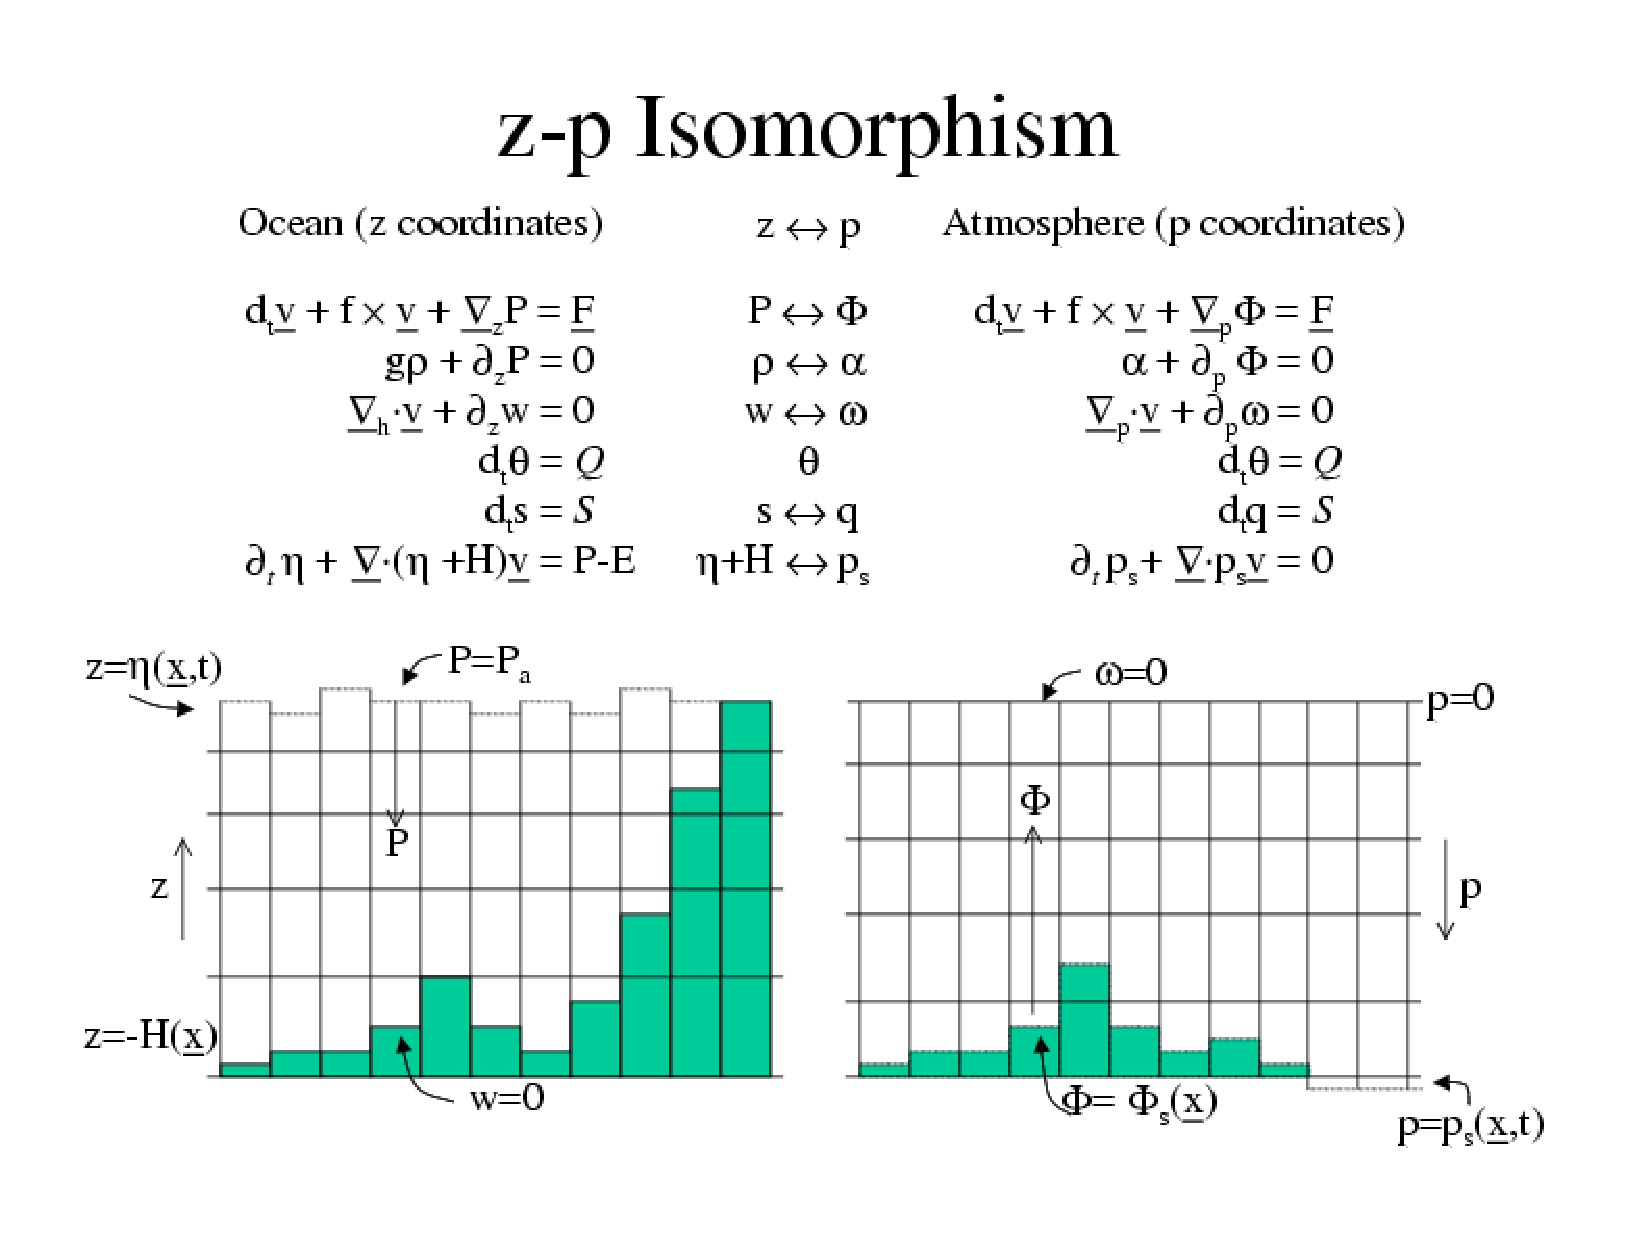
\includegraphics{part1/zandpcoord.eps}
  }
  \end{center}
\caption{Isomorphic equation sets used for atmosphere (right) and
ocean (left).}
\label{fig:isomorphic-equations}
\end{figure}

%%CNHend

The state of the fluid at any time is characterized by the distribution of
velocity $\vec{\mathbf{v}}$, active tracers $\theta $ and $S$, a
`geopotential' $\phi $ and density $\rho =\rho (\theta ,S,p)$ which may
depend on $\theta $, $S$, and $p$. The equations that govern the evolution
of these fields, obtained by applying the laws of classical mechanics and
thermodynamics to a Boussinesq, Navier-Stokes fluid are, written in terms of
a generic vertical coordinate, $r$, so that the appropriate
kinematic boundary conditions can be applied isomorphically
see figure \ref{fig:zandp-vert-coord}.

%%CNHbegin
\begin{figure}
  \begin{center}
   \rotatebox{-90}{
   \resizebox{!}{5.5in}{
   \includegraphics*[2.0in,3.0in][7.5in,10.5in]{part1/vertcoord.eps}
   }
   }
  \end{center}
\caption{Vertical coordinates and kinematic boundary conditions
for atmosphere (top) and ocean (bottom).}
\label{fig:zandp-vert-coord}
\end{figure}

%%CNHend

\begin{equation*}
\frac{D\vec{\mathbf{v}_{h}}}{Dt}+\left( 2\vec{\Omega}\times \vec{\mathbf{v}}
\right) _{h}+\mathbf{\nabla }_{h}\phi =\mathcal{F}_{\vec{\mathbf{v}_{h}}}
\text{ horizontal mtm} \label{eq:horizontal_mtm}
\end{equation*}

\begin{equation}
\frac{D\dot{r}}{Dt}+\widehat{k}\cdot \left( 2\vec{\Omega}\times \vec{\mathbf{
v}}\right) +\frac{\partial \phi }{\partial r}+b=\mathcal{F}_{\dot{r}}\text{
vertical mtm} \label{eq:vertical_mtm}
\end{equation}

\begin{equation}
\mathbf{\nabla }_{h}\cdot \vec{\mathbf{v}}_{h}+\frac{\partial \dot{r}}{
\partial r}=0\text{ continuity}  \label{eq:continuity}
\end{equation}

\begin{equation}
b=b(\theta ,S,r)\text{ equation of state} \label{eq:equation_of_state}
\end{equation}

\begin{equation}
\frac{D\theta }{Dt}=\mathcal{Q}_{\theta }\text{ potential temperature}
\label{eq:potential_temperature}
\end{equation}

\begin{equation}
\frac{DS}{Dt}=\mathcal{Q}_{S}\text{ humidity/salinity}
\label{eq:humidtity_salt}
\end{equation}

Here:

\begin{equation*}
r\text{ is the vertical coordinate}
\end{equation*}

\begin{equation*}
\frac{D}{Dt}=\frac{\partial }{\partial t}+\vec{\mathbf{v}}\cdot \nabla \text{
is the total derivative}
\end{equation*}

\begin{equation*}
\mathbf{\nabla }=\mathbf{\nabla }_{h}+\widehat{k}\frac{\partial }{\partial r}
\text{ is the `grad' operator}
\end{equation*}
with $\mathbf{\nabla }_{h}$ operating in the horizontal and $\widehat{k}
\frac{\partial }{\partial r}$ operating in the vertical, where $\widehat{k}$
is a unit vector in the vertical

\begin{equation*}
t\text{ is time}
\end{equation*}

\begin{equation*}
\vec{\mathbf{v}}=(u,v,\dot{r})=(\vec{\mathbf{v}}_{h},\dot{r})\text{ is the
velocity}
\end{equation*}

\begin{equation*}
\phi \text{ is the `pressure'/`geopotential'}
\end{equation*}

\begin{equation*}
\vec{\Omega}\text{ is the Earth's rotation}
\end{equation*}

\begin{equation*}
b\text{ is the `buoyancy'}
\end{equation*}

\begin{equation*}
\theta \text{ is potential temperature}
\end{equation*}

\begin{equation*}
S\text{ is specific humidity in the atmosphere; salinity in the ocean}
\end{equation*}

\begin{equation*}
\mathcal{F}_{\vec{\mathbf{v}}}\text{ are forcing and dissipation of }\vec{
\mathbf{v}}
\end{equation*}

\begin{equation*}
\mathcal{Q}_{\theta }\mathcal{\ }\text{are forcing and dissipation of }\theta
\end{equation*}

\begin{equation*}
\mathcal{Q}_{S}\mathcal{\ }\text{are forcing and dissipation of }S
\end{equation*}

The $\mathcal{F}^{\prime }s$ and $\mathcal{Q}^{\prime }s$ are provided by
`physics' and forcing packages for atmosphere and ocean. These are described
in later chapters.

\subsection{Kinematic Boundary conditions}

\subsubsection{vertical}

at fixed and moving $r$ surfaces we set (see figure \ref{fig:zandp-vert-coord}):

\begin{equation}
\dot{r}=0atr=R_{fixed}(x,y)\text{ (ocean bottom, top of the atmosphere)}
\label{eq:fixedbc}
\end{equation}

\begin{equation}
\dot{r}=\frac{Dr}{Dt}atr=R_{moving}\text{ \
(oceansurface,bottomoftheatmosphere)}  \label{eq:movingbc}
\end{equation}

Here

\begin{equation*}
R_{moving}=R_{o}+\eta
\end{equation*}
where $R_{o}(x,y)$ is the `$r-$value' (height or pressure, depending on
whether we are in the atmosphere or ocean) of the `moving surface' in the
resting fluid and $\eta $ is the departure from $R_{o}(x,y)$ in the presence
of motion.

\subsubsection{horizontal}

\begin{equation}
\vec{\mathbf{v}}\cdot \vec{\mathbf{n}}=0  \label{eq:noflow}
\end{equation}
where $\vec{\mathbf{n}}$ is the normal to a solid boundary.

\subsection{Atmosphere}

In the atmosphere, (see figure \ref{fig:zandp-vert-coord}), we interpret:

\begin{equation}
r=p\text{ is the pressure}  \label{eq:atmos-r}
\end{equation}

\begin{equation}
\dot{r}=\frac{Dp}{Dt}=\omega \text{ is the vertical velocity in }p\text{
coordinates}  \label{eq:atmos-omega}
\end{equation}

\begin{equation}
\phi =g\,z\text{ is the geopotential height}  \label{eq:atmos-phi}
\end{equation}

\begin{equation}
b=\frac{\partial \Pi }{\partial p}\theta \text{ is the buoyancy}
\label{eq:atmos-b}
\end{equation}

\begin{equation}
\theta =T(\frac{p_{c}}{p})^{\kappa }\text{ is potential temperature}
\label{eq:atmos-theta}
\end{equation}

\begin{equation}
S=q,\text{ is the specific humidity}  \label{eq:atmos-s}
\end{equation}
where

\begin{equation*}
T\text{ is absolute temperature}
\end{equation*}
\begin{equation*}
p\text{ is the pressure}
\end{equation*}
\begin{eqnarray*}
&&z\text{ is the height of the pressure surface} \\
&&g\text{ is the acceleration due to gravity}
\end{eqnarray*}

In the above the ideal gas law, $p=\rho RT$, has been expressed in terms of
the Exner function $\Pi (p)$ given by (see Appendix Atmosphere) 
\begin{equation}
\Pi (p)=c_{p}(\frac{p}{p_{c}})^{\kappa }  \label{eq:exner}
\end{equation}
where $p_{c}$ is a reference pressure and $\kappa =R/c_{p}$ with $R$ the gas
constant and $c_{p}$ the specific heat of air at constant pressure.

At the top of the atmosphere (which is `fixed' in our $r$ coordinate):

\begin{equation*}
R_{fixed}=p_{top}=0
\end{equation*}
In a resting atmosphere the elevation of the mountains at the bottom is
given by 
\begin{equation*}
R_{moving}=R_{o}(x,y)=p_{o}(x,y)
\end{equation*}
i.e. the (hydrostatic) pressure at the top of the mountains in a resting
atmosphere.

The boundary conditions at top and bottom are given by:

\begin{eqnarray}
&&\omega =0~\text{at }r=R_{fixed} \text{ (top of the atmosphere)}
\label{eq:fixed-bc-atmos} \\
\omega &=&\frac{Dp_{s}}{Dt}\text{; at }r=R_{moving}\text{ (bottom of the
atmosphere)}  \label{eq:moving-bc-atmos}
\end{eqnarray}

Then the (hydrostatic form of) equations (\ref{eq:horizontal_mtm}-\ref{eq:humidity_slainty}) 
yields a consistent set of atmospheric equations which, for convenience, are written out in $p$
coordinates in Appendix Atmosphere - see eqs(\ref{eq:atmos-prime}).

\subsection{Ocean}

In the ocean we interpret: 
\begin{eqnarray}
r &=&z\text{ is the height}  \label{eq:ocean-z} \\
\dot{r} &=&\frac{Dz}{Dt}=w\text{ is the vertical velocity}
\label{eq:ocean-w} \\
\phi &=&\frac{p}{\rho _{c}}\text{ is the pressure}  \label{eq:ocean-p} \\
b(\theta ,S,r) &=&\frac{g}{\rho _{c}}\left( \rho (\theta ,S,r)-\rho
_{c}\right) \text{ is the buoyancy}  \label{eq:ocean-b}
\end{eqnarray}
where $\rho _{c}$ is a fixed reference density of water and $g$ is the
acceleration due to gravity.\noindent

In the above

At the bottom of the ocean: $R_{fixed}(x,y)=-H(x,y)$.

The surface of the ocean is given by: $R_{moving}=\eta $

The position of the resting free surface of the ocean is given by $
R_{o}=Z_{o}=0$.

Boundary conditions are:

\begin{eqnarray}
w &=&0~\text{at }r=R_{fixed}\text{ (ocean bottom)}  \label{eq:fixed-bc-ocean}
\\
w &=&\frac{D\eta }{Dt}\text{ at }r=R_{moving}=\eta \text{ (ocean surface) 
\label{eq:moving-bc-ocean}}
\end{eqnarray}
where $\eta $ is the elevation of the free surface.

Then equations (\ref{eq:horizontal_mtm}-\ref{eq:humidity_slainty}) yield a consistent set 
of oceanic equations
which, for convenience, are written out in $z$ coordinates in Appendix Ocean
- see eqs(\ref{eq:ocean-mom}) to (\ref{eq:ocean-salt}).

\subsection{Hydrostatic, Quasi-hydrostatic, Quasi-nonhydrostatic and
Non-hydrostatic forms}

Let us separate $\phi $ in to surface, hydrostatic and non-hydrostatic terms:

\begin{equation}
\phi (x,y,r)=\phi _{s}(x,y)+\phi _{hyd}(x,y,r)+\phi _{nh}(x,y,r)
\label{eq:phi-split}
\end{equation}
and write eq(\ref{eq:incompressible}) in the form:

\begin{equation}
\frac{\partial \vec{\mathbf{v}_{h}}}{\partial t}+\mathbf{\nabla }_{h}\phi
_{s}+\mathbf{\nabla }_{h}\phi _{hyd}+\epsilon _{nh}\mathbf{\nabla }_{h}\phi
_{nh}=\vec{\mathbf{G}}_{\vec{v}_{h}}  \label{eq:mom-h}
\end{equation}

\begin{equation}
\frac{\partial \phi _{hyd}}{\partial r}=-b  \label{eq:hydrostatic}
\end{equation}

\begin{equation}
\epsilon _{nh}\frac{\partial \dot{r}}{\partial t}+\frac{\partial \phi _{nh}}{
\partial r}=G_{\dot{r}}  \label{eq:mom-w}
\end{equation}
Here $\epsilon _{nh}$ is a non-hydrostatic parameter.

The $\left( \vec{\mathbf{G}}_{\vec{v}},G_{\dot{r}}\right) $ in eq(\ref
{eq:mom-h}) and (\ref{eq:mom-w}) represent advective, metric and Coriolis
terms in the momentum equations. In spherical coordinates they take the form
\footnote{
In the hydrostatic primitive equations (\textbf{HPE}) all underlined terms
in (\ref{eq:gu-speherical}), (\ref{eq:gv-spherical}) and (\ref
{eq:gw-spherical}) are omitted; the singly-underlined terms are included in
the quasi-hydrostatic model (\textbf{QH}). The fully non-hydrostatic model (
\textbf{NH}) includes all terms.} - see Marshall et al 1997a for a full
discussion:

\begin{equation}
\left. 
\begin{tabular}{l}
$G_{u}=-\vec{\mathbf{v}}.\nabla u$ \\ 
$-\left\{ \underline{\frac{u\dot{r}}{{r}}}-\frac{uv\tan \varphi}{{r}}\right\} $
\\ 
$-\left\{ -2\Omega v\sin \varphi+\underline{2\Omega \dot{r}\cos \varphi}\right\} $
\\ 
$+\mathcal{F}_{u}$
\end{tabular}
\ \right\} \left\{ 
\begin{tabular}{l}
\textit{advection} \\ 
\textit{metric} \\ 
\textit{Coriolis} \\ 
\textit{\ Forcing/Dissipation}
\end{tabular}
\ \right. \qquad  \label{eq:gu-speherical}
\end{equation}

\begin{equation}
\left. 
\begin{tabular}{l}
$G_{v}=-\vec{\mathbf{v}}.\nabla v$ \\ 
$-\left\{ \underline{\frac{v\dot{r}}{{r}}}-\frac{u^{2}\tan \varphi}{{r}}\right\} 
$ \\ 
$-\left\{ -2\Omega u\sin \varphi \right\} $ \\ 
$+\mathcal{F}_{v}$
\end{tabular}
\ \right\} \left\{ 
\begin{tabular}{l}
\textit{advection} \\ 
\textit{metric} \\ 
\textit{Coriolis} \\ 
\textit{\ Forcing/Dissipation}
\end{tabular}
\ \right. \qquad  \label{eq:gv-spherical}
\end{equation}
\qquad \qquad \qquad \qquad \qquad

\begin{equation}
\left. 
\begin{tabular}{l}
$G_{\dot{r}}=-\underline{\underline{\vec{\mathbf{v}}.\nabla \dot{r}}}$ \\ 
$+\left\{ \underline{\frac{u^{_{^{2}}}+v^{2}}{{r}}}\right\} $ \\ 
${+}\underline{{2\Omega u\cos \varphi}}$ \\ 
$\underline{\underline{\mathcal{F}_{\dot{r}}}}$
\end{tabular}
\ \right\} \left\{ 
\begin{tabular}{l}
\textit{advection} \\ 
\textit{metric} \\ 
\textit{Coriolis} \\ 
\textit{\ Forcing/Dissipation}
\end{tabular}
\ \right.  \label{eq:gw-spherical}
\end{equation}
\qquad \qquad \qquad \qquad \qquad

In the above `${r}$' is the distance from the center of the earth and `$\varphi$
' is latitude.

Grad and div operators in spherical coordinates are defined in appendix
OPERATORS.

%%CNHbegin
\begin{figure}
  \begin{center}
   \resizebox{5in}{!}{
   \includegraphics*[0.5in,0.5in][7.5in,10.5in]{part1/sphere.ps}
   }
  \end{center}
\caption{}
\label{fig:spherical-polar-coord}
\end{figure}

%%CNHend

\subsubsection{Shallow atmosphere approximation}

Most models are based on the `hydrostatic primitive equations' (HPE's) in
which the vertical momentum equation is reduced to a statement of
hydrostatic balance and the `traditional approximation' is made in which the
Coriolis force is treated approximately and the shallow atmosphere
approximation is made.\ The MITgcm need not make the `traditional
approximation'. To be able to support consistent non-hydrostatic forms the
shallow atmosphere approximation can be relaxed - when dividing through by $
r $ in, for example, (\ref{eq:gu-speherical}), we do not replace $r$ by $a$,
the radius of the earth.

\subsubsection{Hydrostatic and quasi-hydrostatic forms}
\label{sec:hydrostatic_and_quasi-hydrostatic_forms}

These are discussed at length in Marshall et al (1997a).

In the `hydrostatic primitive equations' (\textbf{HPE)} all the underlined
terms in Eqs. (\ref{eq:gu-speherical} $\rightarrow $\ \ref{eq:gw-spherical})
are neglected and `${r}$' is replaced by `$a$', the mean radius of the
earth. Once the pressure is found at one level - e.g. by inverting a 2-d
Elliptic equation for $\phi _{s}$ at $r=R_{moving}$ - the pressure can be
computed at all other levels by integration of the hydrostatic relation, eq(
\ref{eq:hydrostatic}).

In the `quasi-hydrostatic' equations (\textbf{QH)} strict balance between
gravity and vertical pressure gradients is not imposed. The $2\Omega u\cos
\varphi $ Coriolis term are not neglected and are balanced by a non-hydrostatic
contribution to the pressure field: only the terms underlined twice in Eqs. (
\ref{eq:gu-speherical}$\rightarrow $\ \ref{eq:gw-spherical}) are set to zero
and, simultaneously, the shallow atmosphere approximation is relaxed. In 
\textbf{QH}\ \textit{all} the metric terms are retained and the full
variation of the radial position of a particle monitored. The \textbf{QH}\
vertical momentum equation (\ref{eq:mom-w}) becomes:

\begin{equation*}
\frac{\partial \phi _{nh}}{\partial r}=2\Omega u\cos \varphi
\end{equation*}
making a small correction to the hydrostatic pressure.

\textbf{QH} has good energetic credentials - they are the same as for 
\textbf{HPE}. Importantly, however, it has the same angular momentum
principle as the full non-hydrostatic model (\textbf{NH)} - see Marshall
et.al., 1997a. As in \textbf{HPE }only a 2-d elliptic problem need be solved.

\subsubsection{Non-hydrostatic and quasi-nonhydrostatic forms}

The MIT model presently supports a full non-hydrostatic ocean isomorph, but
only a quasi-non-hydrostatic atmospheric isomorph.

\paragraph{Non-hydrostatic Ocean}

In the non-hydrostatic ocean model all terms in equations Eqs.(\ref
{eq:gu-speherical} $\rightarrow $\ \ref{eq:gw-spherical}) are retained. A
three dimensional elliptic equation must be solved subject to Neumann
boundary conditions (see below). It is important to note that use of the
full \textbf{NH} does not admit any new `fast' waves in to the system - the
incompressible condition eq(\ref{eq:continuity}) has already filtered out
acoustic modes. It does, however, ensure that the gravity waves are treated
accurately with an exact dispersion relation. The \textbf{NH} set has a
complete angular momentum principle and consistent energetics - see White
and Bromley, 1995; Marshall et.al.\ 1997a.

\paragraph{Quasi-nonhydrostatic Atmosphere}

In the non-hydrostatic version of our atmospheric model we approximate $\dot{
r}$ in the vertical momentum eqs(\ref{eq:mom-w}) and (\ref{eq:gv-spherical})
(but only here) by:

\begin{equation}
\dot{r}=\frac{Dp}{Dt}=\frac{1}{g}\frac{D\phi }{Dt}  \label{eq:quasi-nh-w}
\end{equation}
where $p_{hy}$ is the hydrostatic pressure.

\subsubsection{Summary of equation sets supported by model}

\paragraph{Atmosphere}

Hydrostatic, and quasi-hydrostatic and quasi non-hydrostatic forms of the
compressible non-Boussinesq equations in $p-$coordinates are supported.

\subparagraph{Hydrostatic and quasi-hydrostatic}

The hydrostatic set is written out in $p-$coordinates in appendix Atmosphere
- see eq(\ref{eq:atmos-prime}).

\subparagraph{Quasi-nonhydrostatic}

A quasi-nonhydrostatic form is also supported.

\paragraph{Ocean}

\subparagraph{Hydrostatic and quasi-hydrostatic}

Hydrostatic, and quasi-hydrostatic forms of the incompressible Boussinesq
equations in $z-$coordinates are supported.

\subparagraph{Non-hydrostatic}

Non-hydrostatic forms of the incompressible Boussinesq equations in $z-$
coordinates are supported - see eqs(\ref{eq:ocean-mom}) to (\ref
{eq:ocean-salt}).

\subsection{Solution strategy}

The method of solution employed in the \textbf{HPE}, \textbf{QH} and \textbf{
NH} models is summarized in Figure \ref{fig:solution-strategy}.
Under all dynamics, a 2-d elliptic equation is
first solved to find the surface pressure and the hydrostatic pressure at
any level computed from the weight of fluid above. Under \textbf{HPE} and 
\textbf{QH} dynamics, the horizontal momentum equations are then stepped
forward and $\dot{r}$ found from continuity. Under \textbf{NH} dynamics a
3-d elliptic equation must be solved for the non-hydrostatic pressure before
stepping forward the horizontal momentum equations; $\dot{r}$ is found by
stepping forward the vertical momentum equation.

%%CNHbegin
\begin{figure}
  \begin{center}
   \resizebox{5in}{!}{
   \includegraphics{s_overview/figs/solution_strategy.ps}
   }
  \end{center}
\caption{Basic solution strategy in MITgcm. {\bf HPE} and {\bf QH}
forms diagnose the vertical velocity, in {\bf NH} a prognostic
equation for the vertical velocity is integrated.}
\label{fig:solution-strategy}
\end{figure}

%%CNHend

There is no penalty in implementing \textbf{QH} over \textbf{HPE} except, of
course, some complication that goes with the inclusion of $\cos \varphi \ $
Coriolis terms and the relaxation of the shallow atmosphere approximation.
But this leads to negligible increase in computation. In \textbf{NH}, in
contrast, one additional elliptic equation - a three-dimensional one - must
be inverted for $p_{nh}$. However the `overhead' of the \textbf{NH} model is
essentially negligible in the hydrostatic limit (see detailed discussion in
Marshall et al, 1997) resulting in a non-hydrostatic algorithm that, in the
hydrostatic limit, is as computationally economic as the \textbf{HPEs}.

\subsection{Finding the pressure field}
\label{sec:finding_the_pressure_field}

Unlike the prognostic variables $u$, $v$, $w$, $\theta $ and $S$, the
pressure field must be obtained diagnostically. We proceed, as before, by
dividing the total (pressure/geo) potential in to three parts, a surface
part, $\phi _{s}(x,y)$, a hydrostatic part $\phi _{hyd}(x,y,r)$ and a
non-hydrostatic part $\phi _{nh}(x,y,r)$, as in (\ref{eq:phi-split}), and
writing the momentum equation as in (\ref{eq:mom-h}).

\subsubsection{Hydrostatic pressure}

Hydrostatic pressure is obtained by integrating (\ref{eq:hydrostatic})
vertically from $r=R_{o}$ where $\phi _{hyd}(r=R_{o})=0$, to yield:

\begin{equation*}
\int_{r}^{R_{o}}\frac{\partial \phi _{hyd}}{\partial r}dr=\left[ \phi _{hyd}
\right] _{r}^{R_{o}}=\int_{r}^{R_{o}}-bdr
\end{equation*}
and so

\begin{equation}
\phi _{hyd}(x,y,r)=\int_{r}^{R_{o}}bdr  \label{eq:hydro-phi}
\end{equation}

The model can be easily modified to accommodate a loading term (e.g
atmospheric pressure pushing down on the ocean's surface) by setting:

\begin{equation}
\phi _{hyd}(r=R_{o})=loading  \label{eq:loading}
\end{equation}

\subsubsection{Surface pressure}

The surface pressure equation can be obtained by integrating continuity,
(\ref{eq:continuity}), vertically from $r=R_{fixed}$ to $r=R_{moving}$

\begin{equation*}
\int_{R_{fixed}}^{R_{moving}}\left( \mathbf{\nabla }_{h}\cdot \vec{\mathbf{v}
}_{h}+\partial _{r}\dot{r}\right) dr=0
\end{equation*}

Thus:

\begin{equation*}
\frac{\partial \eta }{\partial t}+\vec{\mathbf{v}}.\nabla \eta
+\int_{R_{fixed}}^{R_{moving}}\mathbf{\nabla }_{h}\cdot \vec{\mathbf{v}}
_{h}dr=0
\end{equation*}
where $\eta =R_{moving}-R_{o}$ is the free-surface $r$-anomaly in units of $
r $. The above can be rearranged to yield, using Leibnitz's theorem:

\begin{equation}
\frac{\partial \eta }{\partial t}+\mathbf{\nabla }_{h}\cdot
\int_{R_{fixed}}^{R_{moving}}\vec{\mathbf{v}}_{h}dr=\text{source}
\label{eq:free-surface}
\end{equation}
where we have incorporated a source term.

Whether $\phi $ is pressure (ocean model, $p/\rho _{c}$) or geopotential
(atmospheric model), in (\ref{eq:mom-h}), the horizontal gradient term can
be written 
\begin{equation}
\mathbf{\nabla }_{h}\phi _{s}=\mathbf{\nabla }_{h}\left( b_{s}\eta \right)
\label{eq:phi-surf}
\end{equation}
where $b_{s}$ is the buoyancy at the surface.

In the hydrostatic limit ($\epsilon _{nh}=0$), equations (\ref{eq:mom-h}), (\ref
{eq:free-surface}) and (\ref{eq:phi-surf}) can be solved by inverting a 2-d
elliptic equation for $\phi _{s}$ as described in Chapter 2. Both `free
surface' and `rigid lid' approaches are available.

\subsubsection{Non-hydrostatic pressure}

Taking the horizontal divergence of (\ref{eq:mom-h}) and adding 
$\frac{\partial }{\partial r}$ of (\ref{eq:mom-w}), invoking the continuity equation
(\ref{eq:continuity}), we deduce that:

\begin{equation}
\nabla _{3}^{2}\phi _{nh}=\nabla .\vec{\mathbf{G}}_{\vec{v}}-\left( \mathbf{
\nabla }_{h}^{2}\phi _{s}+\mathbf{\nabla }^{2}\phi _{hyd}\right) =\nabla .
\vec{\mathbf{F}}  \label{eq:3d-invert}
\end{equation}

For a given rhs this 3-d elliptic equation must be inverted for $\phi _{nh}$
subject to appropriate choice of boundary conditions. This method is usually
called \textit{The Pressure Method} [Harlow and Welch, 1965; Williams, 1969;
Potter, 1976]. In the hydrostatic primitive equations case (\textbf{HPE}),
the 3-d problem does not need to be solved.

\paragraph{Boundary Conditions}

We apply the condition of no normal flow through all solid boundaries - the
coasts (in the ocean) and the bottom:

\begin{equation}
\vec{\mathbf{v}}.\widehat{n}=0  \label{nonormalflow}
\end{equation}
where $\widehat{n}$ is a vector of unit length normal to the boundary. The
kinematic condition (\ref{nonormalflow}) is also applied to the vertical
velocity at $r=R_{moving}$. No-slip $\left( v_{T}=0\right) \ $or slip $
\left( \partial v_{T}/\partial n=0\right) \ $conditions are employed on the
tangential component of velocity, $v_{T}$, at all solid boundaries,
depending on the form chosen for the dissipative terms in the momentum
equations - see below.

Eq.(\ref{nonormalflow}) implies, making use of (\ref{eq:mom-h}), that:

\begin{equation}
\widehat{n}.\nabla \phi _{nh}=\widehat{n}.\vec{\mathbf{F}}
\label{eq:inhom-neumann-nh}
\end{equation}
where

\begin{equation*}
\vec{\mathbf{F}}=\vec{\mathbf{G}}_{\vec{v}}-\left( \mathbf{\nabla }_{h}\phi
_{s}+\mathbf{\nabla }\phi _{hyd}\right) 
\end{equation*}
presenting inhomogeneous Neumann boundary conditions to the Elliptic problem
(\ref{eq:3d-invert}). As shown, for example, by Williams (1969), one can
exploit classical 3D potential theory and, by introducing an appropriately
chosen $\delta $-function sheet of `source-charge', replace the
inhomogeneous boundary condition on pressure by a homogeneous one. The
source term $rhs$ in (\ref{eq:3d-invert}) is the divergence of the vector $
\vec{\mathbf{F}}.$ By simultaneously setting $
\begin{array}{l}
\widehat{n}.\vec{\mathbf{F}}
\end{array}
=0$\ and $\widehat{n}.\nabla \phi _{nh}=0\ $on the boundary the following
self-consistent but simpler homogenized Elliptic problem is obtained:

\begin{equation*}
\nabla ^{2}\phi _{nh}=\nabla .\widetilde{\vec{\mathbf{F}}}\qquad
\end{equation*}
where $\widetilde{\vec{\mathbf{F}}}$ is a modified $\vec{\mathbf{F}}$ such
that $\widetilde{\vec{\mathbf{F}}}.\widehat{n}=0$. As is implied by (\ref
{eq:inhom-neumann-nh}) the modified boundary condition becomes:

\begin{equation}
\widehat{n}.\nabla \phi _{nh}=0  \label{eq:hom-neumann-nh}
\end{equation}

If the flow is `close' to hydrostatic balance then the 3-d inversion
converges rapidly because $\phi _{nh}\ $is then only a small correction to
the hydrostatic pressure field (see the discussion in Marshall et al, a,b).

The solution $\phi _{nh}\ $to (\ref{eq:3d-invert}) and (\ref{eq:inhom-neumann-nh})
does not vanish at $r=R_{moving}$, and so refines the pressure there.

\subsection{Forcing/dissipation}

\subsubsection{Forcing}

The forcing terms $\mathcal{F}$ on the rhs of the equations are provided by
`physics packages' and forcing packages. These are described later on.

\subsubsection{Dissipation}

\paragraph{Momentum}

Many forms of momentum dissipation are available in the model. Laplacian and
biharmonic frictions are commonly used:

\begin{equation}
D_{V}=A_{h}\nabla _{h}^{2}v+A_{v}\frac{\partial ^{2}v}{\partial z^{2}}
+A_{4}\nabla _{h}^{4}v  \label{eq:dissipation}
\end{equation}
where $A_{h}$ and $A_{v}\ $are (constant) horizontal and vertical viscosity
coefficients and $A_{4}\ $is the horizontal coefficient for biharmonic
friction. These coefficients are the same for all velocity components.

\paragraph{Tracers}

The mixing terms for the temperature and salinity equations have a similar
form to that of momentum except that the diffusion tensor can be
non-diagonal and have varying coefficients. $\qquad $
\begin{equation}
D_{T,S}=\nabla .[\underline{\underline{K}}\nabla (T,S)]+K_{4}\nabla
_{h}^{4}(T,S)  \label{eq:diffusion}
\end{equation}
where $\underline{\underline{K}}\ $is the diffusion tensor and the $K_{4}\ $
horizontal coefficient for biharmonic diffusion. In the simplest case where
the subgrid-scale fluxes of heat and salt are parameterized with constant
horizontal and vertical diffusion coefficients, $\underline{\underline{K}}$,
reduces to a diagonal matrix with constant coefficients:

\begin{equation}
\qquad \qquad \qquad \qquad K=\left( 
\begin{array}{ccc}
K_{h} & 0 & 0 \\ 
0 & K_{h} & 0 \\ 
0 & 0 & K_{v}
\end{array}
\right) \qquad \qquad \qquad  \label{eq:diagonal-diffusion-tensor}
\end{equation}
where $K_{h}\ $and $K_{v}\ $are the horizontal and vertical diffusion
coefficients. These coefficients are the same for all tracers (temperature,
salinity ... ).

\subsection{Vector invariant form}

For some purposes it is advantageous to write momentum advection in eq(\ref
{eq:horizontal_mtm}) and (\ref{eq:vertical_mtm}) in the (so-called) `vector invariant' form:

\begin{equation}
\frac{D\vec{\mathbf{v}}}{Dt}=\frac{\partial \vec{\mathbf{v}}}{\partial t}
+\left( \nabla \times \vec{\mathbf{v}}\right) \times \vec{\mathbf{v}}+\nabla 
\left[ \frac{1}{2}(\vec{\mathbf{v}}\cdot \vec{\mathbf{v}})\right]
\label{eq:vi-identity}
\end{equation}
This permits alternative numerical treatments of the non-linear terms based
on their representation as a vorticity flux. Because gradients of coordinate
vectors no longer appear on the rhs of (\ref{eq:vi-identity}), explicit
representation of the metric terms in (\ref{eq:gu-speherical}), (\ref
{eq:gv-spherical}) and (\ref{eq:gw-spherical}), can be avoided: information
about the geometry is contained in the areas and lengths of the volumes used
to discretize the model.

\subsection{Adjoint}

Tangent linear and adjoint counterparts of the forward model are described
in Chapter 5.

% $Header: /u/gcmpack/manual/s_overview/text/manual.tex,v 1.8 2001/10/25 15:24:01 cnh Exp $
% $Name:  $

\section{Appendix ATMOSPHERE}

\subsection{Hydrostatic Primitive Equations for the Atmosphere in pressure
coordinates}

\label{sect-hpe-p}

The hydrostatic primitive equations (HPEs) in p-coordinates are: 
\begin{eqnarray}
\frac{D\vec{\mathbf{v}}_{h}}{Dt}+f\hat{\mathbf{k}}\times \vec{\mathbf{v}}
_{h}+\mathbf{\nabla }_{p}\phi &=&\vec{\mathbf{\mathcal{F}}}
\label{eq:atmos-mom} \\
\frac{\partial \phi }{\partial p}+\alpha &=&0  \label{eq-p-hydro-start} \\
\mathbf{\nabla }_{p}\cdot \vec{\mathbf{v}}_{h}+\frac{\partial \omega }{
\partial p} &=&0  \label{eq:atmos-cont} \\
p\alpha &=&RT  \label{eq:atmos-eos} \\
c_{v}\frac{DT}{Dt}+p\frac{D\alpha }{Dt} &=&\mathcal{Q}  \label{eq:atmos-heat}
\end{eqnarray}
where $\vec{\mathbf{v}}_{h}=(u,v,0)$ is the `horizontal' (on pressure
surfaces) component of velocity,$\frac{D}{Dt}=\vec{\mathbf{v}}_{h}\cdot 
\mathbf{\nabla }_{p}+\omega \frac{\partial }{\partial p}$ is the total
derivative, $f=2\Omega \sin \varphi$ is the Coriolis parameter, $\phi =gz$ is
the geopotential, $\alpha =1/\rho $ is the specific volume, $\omega =\frac{Dp
}{Dt}$ is the vertical velocity in the $p-$coordinate. Equation(\ref
{eq:atmos-heat}) is the first law of thermodynamics where internal energy $
e=c_{v}T$, $T$ is temperature, $Q$ is the rate of heating per unit mass and $
p\frac{D\alpha }{Dt}$ is the work done by the fluid in compressing.

It is convenient to cast the heat equation in terms of potential temperature 
$\theta $ so that it looks more like a generic conservation law.
Differentiating (\ref{eq:atmos-eos}) we get: 
\begin{equation*}
p\frac{D\alpha }{Dt}+\alpha \frac{Dp}{Dt}=R\frac{DT}{Dt}
\end{equation*}
which, when added to the heat equation (\ref{eq:atmos-heat}) and using $
c_{p}=c_{v}+R$, gives: 
\begin{equation}
c_{p}\frac{DT}{Dt}-\alpha \frac{Dp}{Dt}=\mathcal{Q}
\label{eq-p-heat-interim}
\end{equation}
Potential temperature is defined: 
\begin{equation}
\theta =T(\frac{p_{c}}{p})^{\kappa }  \label{eq:potential-temp}
\end{equation}
where $p_{c}$ is a reference pressure and $\kappa =R/c_{p}$. For convenience
we will make use of the Exner function $\Pi (p)$ which defined by: 
\begin{equation}
\Pi (p)=c_{p}(\frac{p}{p_{c}})^{\kappa }  \label{Exner}
\end{equation}
The following relations will be useful and are easily expressed in terms of
the Exner function: 
\begin{equation*}
c_{p}T=\Pi \theta \;\;;\;\;\frac{\partial \Pi }{\partial p}=\frac{\kappa \Pi 
}{p}\;\;;\;\;\alpha =\frac{\kappa \Pi \theta }{p}=\frac{\partial \ \Pi }{
\partial p}\theta \;\;;\;\;\frac{D\Pi }{Dt}=\frac{\partial \Pi }{\partial p}
\frac{Dp}{Dt}
\end{equation*}
where $b=\frac{\partial \ \Pi }{\partial p}\theta $ is the buoyancy.

The heat equation is obtained by noting that 
\begin{equation*}
c_{p}\frac{DT}{Dt}=\frac{D(\Pi \theta )}{Dt}=\Pi \frac{D\theta }{Dt}+\theta 
\frac{D\Pi }{Dt}=\Pi \frac{D\theta }{Dt}+\alpha \frac{Dp}{Dt}
\end{equation*}
and on substituting into (\ref{eq-p-heat-interim}) gives: 
\begin{equation}
\Pi \frac{D\theta }{Dt}=\mathcal{Q}
\label{eq:potential-temperature-equation}
\end{equation}
which is in conservative form.

For convenience in the model we prefer to step forward (\ref
{eq:potential-temperature-equation}) rather than (\ref{eq:atmos-heat}).

\subsubsection{Boundary conditions}

The upper and lower boundary conditions are : 
\begin{eqnarray}
\mbox{at the top:}\;\;p=0 &&\text{, }\omega =\frac{Dp}{Dt}=0 \\
\mbox{at the surface:}\;\;p=p_{s} &&\text{, }\phi =\phi _{topo}=g~Z_{topo}
\label{eq:boundary-condition-atmosphere}
\end{eqnarray}
In $p$-coordinates, the upper boundary acts like a solid boundary ($\omega
=0 $); in $z$-coordinates and the lower boundary is analogous to a free
surface ($\phi $ is imposed and $\omega \neq 0$).

\subsubsection{Splitting the geo-potential}

For the purposes of initialization and reducing round-off errors, the model
deals with perturbations from reference (or ``standard'') profiles. For
example, the hydrostatic geopotential associated with the resting atmosphere
is not dynamically relevant and can therefore be subtracted from the
equations. The equations written in terms of perturbations are obtained by
substituting the following definitions into the previous model equations: 
\begin{eqnarray}
\theta &=&\theta _{o}+\theta ^{\prime }  \label{eq:atmos-ref-prof-theta} \\
\alpha &=&\alpha _{o}+\alpha ^{\prime }  \label{eq:atmos-ref-prof-alpha} \\
\phi &=&\phi _{o}+\phi ^{\prime }  \label{eq:atmos-ref-prof-phi}
\end{eqnarray}
The reference state (indicated by subscript ``0'') corresponds to
horizontally homogeneous atmosphere at rest ($\theta _{o},\alpha _{o},\phi
_{o}$) with surface pressure $p_{o}(x,y)$ that satisfies $\phi
_{o}(p_{o})=g~Z_{topo}$, defined: 
\begin{eqnarray*}
\theta _{o}(p) &=&f^{n}(p) \\
\alpha _{o}(p) &=&\Pi _{p}\theta _{o} \\
\phi _{o}(p) &=&\phi _{topo}-\int_{p_{0}}^{p}\alpha _{o}dp
\end{eqnarray*}
%\begin{eqnarray*}
%\phi'_\alpha & = & \int^p_{p_o} (\alpha_o -\alpha) dp \\
%\phi'_s(x,y,t) & = & \int_{p_o}^{p_s} \alpha dp
%\end{eqnarray*}

The final form of the HPE's in p coordinates is then: 
\begin{eqnarray}
\frac{D\vec{\mathbf{v}}_{h}}{Dt}+f\hat{\mathbf{k}}\times \vec{\mathbf{v}}
_{h}+\mathbf{\nabla }_{p}\phi ^{\prime } &=&\vec{\mathbf{\mathcal{F}}} \label{eq:atmos-prime} \\
\frac{\partial \phi ^{\prime }}{\partial p}+\alpha ^{\prime } &=&0 \\
\mathbf{\nabla }_{p}\cdot \vec{\mathbf{v}}_{h}+\frac{\partial \omega }{
\partial p} &=&0 \\
\frac{\partial \Pi }{\partial p}\theta ^{\prime } &=&\alpha ^{\prime } \\
\frac{D\theta }{Dt} &=&\frac{\mathcal{Q}}{\Pi } 
\end{eqnarray}

% $Header: /u/gcmpack/manual/s_overview/text/manual.tex,v 1.8 2001/10/25 15:24:01 cnh Exp $
% $Name:  $

\section{Appendix OCEAN}

\subsection{Equations of motion for the ocean}

We review here the method by which the standard (Boussinesq, incompressible)
HPE's for the ocean written in z-coordinates are obtained. The
non-Boussinesq equations for oceanic motion are: 
\begin{eqnarray}
\frac{D\vec{\mathbf{v}}_{h}}{Dt}+f\hat{\mathbf{k}}\times \vec{\mathbf{v}}
_{h}+\frac{1}{\rho }\mathbf{\nabla }_{z}p &=&\vec{\mathbf{\mathcal{F}}} \\
\epsilon _{nh}\frac{Dw}{Dt}+g+\frac{1}{\rho }\frac{\partial p}{\partial z}
&=&\epsilon _{nh}\mathcal{F}_{w} \\
\frac{1}{\rho }\frac{D\rho }{Dt}+\mathbf{\nabla }_{z}\cdot \vec{\mathbf{v}}
_{h}+\frac{\partial w}{\partial z} &=&0 \label{eq-zns-cont}\\
\rho &=&\rho (\theta ,S,p) \label{eq-zns-eos}\\
\frac{D\theta }{Dt} &=&\mathcal{Q}_{\theta } \label{eq-zns-heat}\\
\frac{DS}{Dt} &=&\mathcal{Q}_{s}  \label{eq-zns-salt}
\label{eq:non-boussinesq}
\end{eqnarray}
These equations permit acoustics modes, inertia-gravity waves,
non-hydrostatic motions, a geostrophic (Rossby) mode and a thermo-haline
mode. As written, they cannot be integrated forward consistently - if we
step $\rho $ forward in (\ref{eq-zns-cont}), the answer will not be
consistent with that obtained by stepping (\ref{eq-zns-heat}) and (\ref
{eq-zns-salt}) and then using (\ref{eq-zns-eos}) to yield $\rho $. It is
therefore necessary to manipulate the system as follows. Differentiating the
EOS (equation of state) gives:

\begin{equation}
\frac{D\rho }{Dt}=\left. \frac{\partial \rho }{\partial \theta }\right|
_{S,p}\frac{D\theta }{Dt}+\left. \frac{\partial \rho }{\partial S}\right|
_{\theta ,p}\frac{DS}{Dt}+\left. \frac{\partial \rho }{\partial p}\right|
_{\theta ,S}\frac{Dp}{Dt}  \label{EOSexpansion}
\end{equation}

Note that $\frac{\partial \rho }{\partial p}=\frac{1}{c_{s}^{2}}$ is the
reciprocal of the sound speed ($c_{s}$) squared. Substituting into \ref{eq-zns-cont} gives: 
\begin{equation}
\frac{1}{\rho c_{s}^{2}}\frac{Dp}{Dt}+\mathbf{\nabla }_{z}\cdot \vec{\mathbf{
v}}+\partial _{z}w\approx 0  \label{eq-zns-pressure}
\end{equation}
where we have used an approximation sign to indicate that we have assumed
adiabatic motion, dropping the $\frac{D\theta }{Dt}$ and $\frac{DS}{Dt}$.
Replacing \ref{eq-zns-cont} with \ref{eq-zns-pressure} yields a system that
can be explicitly integrated forward: 
\begin{eqnarray}
\frac{D\vec{\mathbf{v}}_{h}}{Dt}+f\hat{\mathbf{k}}\times \vec{\mathbf{v}}
_{h}+\frac{1}{\rho }\mathbf{\nabla }_{z}p &=&\vec{\mathbf{\mathcal{F}}}
\label{eq-cns-hmom} \\
\epsilon _{nh}\frac{Dw}{Dt}+g+\frac{1}{\rho }\frac{\partial p}{\partial z}
&=&\epsilon _{nh}\mathcal{F}_{w}  \label{eq-cns-hydro} \\
\frac{1}{\rho c_{s}^{2}}\frac{Dp}{Dt}+\mathbf{\nabla }_{z}\cdot \vec{\mathbf{
v}}_{h}+\frac{\partial w}{\partial z} &=&0  \label{eq-cns-cont} \\
\rho &=&\rho (\theta ,S,p)  \label{eq-cns-eos} \\
\frac{D\theta }{Dt} &=&\mathcal{Q}_{\theta }  \label{eq-cns-heat} \\
\frac{DS}{Dt} &=&\mathcal{Q}_{s}  \label{eq-cns-salt}
\end{eqnarray}

\subsubsection{Compressible z-coordinate equations}

Here we linearize the acoustic modes by replacing $\rho $ with $\rho _{o}(z)$
wherever it appears in a product (ie. non-linear term) - this is the
`Boussinesq assumption'. The only term that then retains the full variation
in $\rho $ is the gravitational acceleration: 
\begin{eqnarray}
\frac{D\vec{\mathbf{v}}_{h}}{Dt}+f\hat{\mathbf{k}}\times \vec{\mathbf{v}}
_{h}+\frac{1}{\rho _{o}}\mathbf{\nabla }_{z}p &=&\vec{\mathbf{\mathcal{F}}}
\label{eq-zcb-hmom} \\
\epsilon _{nh}\frac{Dw}{Dt}+\frac{g\rho }{\rho _{o}}+\frac{1}{\rho _{o}}
\frac{\partial p}{\partial z} &=&\epsilon _{nh}\mathcal{F}_{w}
\label{eq-zcb-hydro} \\
\frac{1}{\rho _{o}c_{s}^{2}}\frac{Dp}{Dt}+\mathbf{\nabla }_{z}\cdot \vec{
\mathbf{v}}_{h}+\frac{\partial w}{\partial z} &=&0  \label{eq-zcb-cont} \\
\rho &=&\rho (\theta ,S,p)  \label{eq-zcb-eos} \\
\frac{D\theta }{Dt} &=&\mathcal{Q}_{\theta }  \label{eq-zcb-heat} \\
\frac{DS}{Dt} &=&\mathcal{Q}_{s}  \label{eq-zcb-salt}
\end{eqnarray}
These equations still retain acoustic modes. But, because the
``compressible'' terms are linearized, the pressure equation \ref
{eq-zcb-cont} can be integrated implicitly with ease (the time-dependent
term appears as a Helmholtz term in the non-hydrostatic pressure equation).
These are the \emph{truly} compressible Boussinesq equations. Note that the
EOS must have the same pressure dependency as the linearized pressure term,
ie. $\left. \frac{\partial \rho }{\partial p}\right| _{\theta ,S}=\frac{1}{
c_{s}^{2}}$, for consistency.

\subsubsection{`Anelastic' z-coordinate equations}

The anelastic approximation filters the acoustic mode by removing the
time-dependency in the continuity (now pressure-) equation (\ref{eq-zcb-cont}
). This could be done simply by noting that $\frac{Dp}{Dt}\approx -g\rho _{o}
\frac{Dz}{Dt}=-g\rho _{o}w$, but this leads to an inconsistency between
continuity and EOS. A better solution is to change the dependency on
pressure in the EOS by splitting the pressure into a reference function of
height and a perturbation: 
\begin{equation*}
\rho =\rho (\theta ,S,p_{o}(z)+\epsilon _{s}p^{\prime })
\end{equation*}
Remembering that the term $\frac{Dp}{Dt}$ in continuity comes from
differentiating the EOS, the continuity equation then becomes: 
\begin{equation*}
\frac{1}{\rho _{o}c_{s}^{2}}\left( \frac{Dp_{o}}{Dt}+\epsilon _{s}\frac{
Dp^{\prime }}{Dt}\right) +\mathbf{\nabla }_{z}\cdot \vec{\mathbf{v}}_{h}+
\frac{\partial w}{\partial z}=0
\end{equation*}
If the time- and space-scales of the motions of interest are longer than
those of acoustic modes, then $\frac{Dp^{\prime }}{Dt}<<(\frac{Dp_{o}}{Dt},
\mathbf{\nabla }\cdot \vec{\mathbf{v}}_{h})$ in the continuity equations and 
$\left. \frac{\partial \rho }{\partial p}\right| _{\theta ,S}\frac{
Dp^{\prime }}{Dt}<<\left. \frac{\partial \rho }{\partial p}\right| _{\theta
,S}\frac{Dp_{o}}{Dt}$ in the EOS (\ref{EOSexpansion}). Thus we set $\epsilon
_{s}=0$, removing the dependency on $p^{\prime }$ in the continuity equation
and EOS. Expanding $\frac{Dp_{o}(z)}{Dt}=-g\rho _{o}w$ then leads to the
anelastic continuity equation: 
\begin{equation}
\mathbf{\nabla }_{z}\cdot \vec{\mathbf{v}}_{h}+\frac{\partial w}{\partial z}-
\frac{g}{c_{s}^{2}}w=0  \label{eq-za-cont1}
\end{equation}
A slightly different route leads to the quasi-Boussinesq continuity equation
where we use the scaling $\frac{\partial \rho ^{\prime }}{\partial t}+
\mathbf{\nabla }_{3}\cdot \rho ^{\prime }\vec{\mathbf{v}}<<\mathbf{\nabla }
_{3}\cdot \rho _{o}\vec{\mathbf{v}}$ yielding: 
\begin{equation}
\mathbf{\nabla }_{z}\cdot \vec{\mathbf{v}}_{h}+\frac{1}{\rho _{o}}\frac{
\partial \left( \rho _{o}w\right) }{\partial z}=0  \label{eq-za-cont2}
\end{equation}
Equations \ref{eq-za-cont1} and \ref{eq-za-cont2} are in fact the same
equation if: 
\begin{equation}
\frac{1}{\rho _{o}}\frac{\partial \rho _{o}}{\partial z}=\frac{-g}{c_{s}^{2}}
\end{equation}
Again, note that if $\rho _{o}$ is evaluated from prescribed $\theta _{o}$
and $S_{o}$ profiles, then the EOS dependency on $p_{o}$ and the term $\frac{
g}{c_{s}^{2}}$ in continuity should be referred to those same profiles. The
full set of `quasi-Boussinesq' or `anelastic' equations for the ocean are
then: 
\begin{eqnarray}
\frac{D\vec{\mathbf{v}}_{h}}{Dt}+f\hat{\mathbf{k}}\times \vec{\mathbf{v}}
_{h}+\frac{1}{\rho _{o}}\mathbf{\nabla }_{z}p &=&\vec{\mathbf{\mathcal{F}}}
\label{eq-zab-hmom} \\
\epsilon _{nh}\frac{Dw}{Dt}+\frac{g\rho }{\rho _{o}}+\frac{1}{\rho _{o}}
\frac{\partial p}{\partial z} &=&\epsilon _{nh}\mathcal{F}_{w}
\label{eq-zab-hydro} \\
\mathbf{\nabla }_{z}\cdot \vec{\mathbf{v}}_{h}+\frac{1}{\rho _{o}}\frac{
\partial \left( \rho _{o}w\right) }{\partial z} &=&0  \label{eq-zab-cont} \\
\rho &=&\rho (\theta ,S,p_{o}(z))  \label{eq-zab-eos} \\
\frac{D\theta }{Dt} &=&\mathcal{Q}_{\theta }  \label{eq-zab-heat} \\
\frac{DS}{Dt} &=&\mathcal{Q}_{s}  \label{eq-zab-salt}
\end{eqnarray}

\subsubsection{Incompressible z-coordinate equations}

Here, the objective is to drop the depth dependence of $\rho _{o}$ and so,
technically, to also remove the dependence of $\rho $ on $p_{o}$. This would
yield the ``truly'' incompressible Boussinesq equations: 
\begin{eqnarray}
\frac{D\vec{\mathbf{v}}_{h}}{Dt}+f\hat{\mathbf{k}}\times \vec{\mathbf{v}}
_{h}+\frac{1}{\rho _{c}}\mathbf{\nabla }_{z}p &=&\vec{\mathbf{\mathcal{F}}}
\label{eq-ztb-hmom} \\
\epsilon _{nh}\frac{Dw}{Dt}+\frac{g\rho }{\rho _{c}}+\frac{1}{\rho _{c}}
\frac{\partial p}{\partial z} &=&\epsilon _{nh}\mathcal{F}_{w}
\label{eq-ztb-hydro} \\
\mathbf{\nabla }_{z}\cdot \vec{\mathbf{v}}_{h}+\frac{\partial w}{\partial z}
&=&0  \label{eq-ztb-cont} \\
\rho &=&\rho (\theta ,S)  \label{eq-ztb-eos} \\
\frac{D\theta }{Dt} &=&\mathcal{Q}_{\theta }  \label{eq-ztb-heat} \\
\frac{DS}{Dt} &=&\mathcal{Q}_{s}  \label{eq-ztb-salt}
\end{eqnarray}
where $\rho _{c}$ is a constant reference density of water.

\subsubsection{Compressible non-divergent equations}

The above ``incompressible'' equations are incompressible in both the flow
and the density. In many oceanic applications, however, it is important to
retain compressibility effects in the density. To do this we must split the
density thus: 
\begin{equation*}
\rho =\rho _{o}+\rho ^{\prime }
\end{equation*}
We then assert that variations with depth of $\rho _{o}$ are unimportant
while the compressible effects in $\rho ^{\prime }$ are: 
\begin{equation*}
\rho _{o}=\rho _{c}
\end{equation*}
\begin{equation*}
\rho ^{\prime }=\rho (\theta ,S,p_{o}(z))-\rho _{o}
\end{equation*}
This then yields what we can call the semi-compressible Boussinesq
equations: 
\begin{eqnarray}
\frac{D\vec{\mathbf{v}}_{h}}{Dt}+f\hat{\mathbf{k}}\times \vec{\mathbf{v}}
_{h}+\frac{1}{\rho _{c}}\mathbf{\nabla }_{z}p^{\prime } &=&\vec{\mathbf{
\mathcal{F}}}  \label{eq:ocean-mom} \\
\epsilon _{nh}\frac{Dw}{Dt}+\frac{g\rho ^{\prime }}{\rho _{c}}+\frac{1}{\rho
_{c}}\frac{\partial p^{\prime }}{\partial z} &=&\epsilon _{nh}\mathcal{F}_{w}
\label{eq:ocean-wmom} \\
\mathbf{\nabla }_{z}\cdot \vec{\mathbf{v}}_{h}+\frac{\partial w}{\partial z}
&=&0  \label{eq:ocean-cont} \\
\rho ^{\prime } &=&\rho (\theta ,S,p_{o}(z))-\rho _{c}  \label{eq:ocean-eos}
\\
\frac{D\theta }{Dt} &=&\mathcal{Q}_{\theta }  \label{eq:ocean-theta} \\
\frac{DS}{Dt} &=&\mathcal{Q}_{s}  \label{eq:ocean-salt}
\end{eqnarray}
Note that the hydrostatic pressure of the resting fluid, including that
associated with $\rho _{c}$, is subtracted out since it has no effect on the
dynamics.

Though necessary, the assumptions that go into these equations are messy
since we essentially assume a different EOS for the reference density and
the perturbation density. Nevertheless, it is the hydrostatic ($\epsilon
_{nh}=0$ form of these equations that are used throughout the ocean modeling
community and referred to as the primitive equations (HPE).

% $Header: /u/gcmpack/manual/s_overview/text/manual.tex,v 1.8 2001/10/25 15:24:01 cnh Exp $
% $Name:  $

\section{Appendix:OPERATORS}

\subsection{Coordinate systems}

\subsubsection{Spherical coordinates}

In spherical coordinates, the velocity components in the zonal, meridional
and vertical direction respectively, are given by (see Fig.2) :

\begin{equation*}
u=r\cos \varphi \frac{D\lambda }{Dt}
\end{equation*}

\begin{equation*}
v=r\frac{D\varphi }{Dt}\qquad
\end{equation*}
$\qquad \qquad \qquad \qquad $

\begin{equation*}
\dot{r}=\frac{Dr}{Dt}
\end{equation*}

Here $\varphi $ is the latitude, $\lambda $ the longitude, $r$ the radial
distance of the particle from the center of the earth, $\Omega $ is the
angular speed of rotation of the Earth and $D/Dt$ is the total derivative.

The `grad' ($\nabla $) and `div' ($\nabla $.) operators are defined by, in
spherical coordinates:

\begin{equation*}
\nabla \equiv \left( \frac{1}{r\cos \varphi }\frac{\partial }{\partial \lambda }
,\frac{1}{r}\frac{\partial }{\partial \varphi },\frac{\partial }{\partial r}
\right)
\end{equation*}

\begin{equation*}
\nabla .v\equiv \frac{1}{r\cos \varphi }\left\{ \frac{\partial u}{\partial
\lambda }+\frac{\partial }{\partial \varphi }\left( v\cos \varphi \right) \right\}
+\frac{1}{r^{2}}\frac{\partial \left( r^{2}\dot{r}\right) }{\partial r}
\end{equation*}

%tci%\end{document}

%%%% % $Header: /u/gcmpack/manual/s_overview/Attic/introduction.tex,v 1.1.1.1 2001/08/08 16:16:16 adcroft Exp $
% $Name:  $

\section{Introduction}

This documentation provides the reader with the information necessary to
carry out numerical experiments using MITgcm. It gives a comprehensive
description of the continuous equations on which the model is based, the
numerical algorithms the model employs and a description of the associated
program code. Along with the hydrodynamical kernel, physical and
biogeochemical parameterizations of key atmospheric and oceanic processes
are available. A number of examples illustrating the use of the model in
both process and general circulation studies of the atmosphere and ocean are
also presented.

MITgcm has a number of novel aspects:

\begin{itemize}
\item  it can be used to study both atmospheric and oceanic phenomena; one
hydrodynamical kernel is used to drive forward both atmospheric and oceanic
models - see fig.1%
\marginpar{
Fig.1 One model}\ref{fig:onemodel}

\item  it has a non-hydrostatic capability and so can be used to study both
small-scale and large scale processes - see fig.2%
\marginpar{
Fig.2 All scales}\ref{fig:all-scales}

\item  finite volume techniques are employed yielding an intuitive
discretization and support for the treatment of irregular geometries using
orthogonal curvilinear grids and shaved cells - see fig.3%
\marginpar{
Fig.3 Finite volumes}\ref{fig:Finite volumes}

\item  tangent linear and adjoint counterparts are automatically maintained
along with the forward model, permitting sensitivity and optimization
studies.

\item  the model is developed to perform efficiently on a wide variety of
computational platforms.
\end{itemize}

Key publications reporting on and charting the development of the model are
listed in Appendix Refs.

We begin by briefly showing some of the results of the model in action to
give a feel for the wide range of problems that can be addressed using it.

%%%% % $Header: /u/gcmpack/manual/s_overview/Attic/illustration.tex,v 1.1.1.1 2001/08/08 16:16:16 adcroft Exp $
% $Name:  $

\section{Illustrations of the model in action}

The MITgcm has been designed and used to model a vast range of phenomena,
from convection on the scale of meters in the ocean to the global pattern of
atmospheric winds - see fig.2\ref{fig:all-scales}. To give a flavor of the
kinds of problems the model has been used to study, we briefly describe some
of them here. A more detailed description of the underlying formulation,
numerical algorithm and implementation that lie behind these calculations is
given later. Indeed it is easy to reproduce the results shown here: simply
download the model (the minimum you need is a PC running linux, together
with a FORTRAN\ 77 compiler) and follow the examples.

\subsection{Global atmosphere: `Held-Suarez' benchmark}

Fig.E1a.\ref{fig:Held-Suarez} is an instaneous plot of the 500$mb$ height
field obtained using a 5-level version of the atmospheric pressure isomorph
run at 300$km$ resolution. We see fully developed baroclinic eddies along
the northern hemisphere storm track. There are no mountains (but you can
easily put them in) or land-sea contrast. The model is driven by relaxation
to a radiative-convective equilibrium profile, following the description set
out in Held and Suarez; 1994 designed to test atmospheric hydrodynamical
cores - there are no mountains or land-sea contrast. As decribed in Adcroft
(2001), `cubed sphere' is used to descretize the globe permitting a uniform
gridding and obviated the need to fourier filter.

Fig.E1b shows the 5-year mean, zonally averaged potential temperature, zonal
wind and meridional overturning streamfunction from the 5-level model.

A regular spherical lat-lon grid can also be used.

Results from this integration, together with a 20-level calculation, can be
found here - link through to channel.

This calculation takes 1 day of computation per year of intergation on a
pentium IV PC.

\subsection{Ocean gyres}

\subsection{Global ocean circulation}

Fig.E2a shows the pattern of ocean currents at the surface of a 4$^{\circ }$
global ocean model run with 15 vertical levels. The model is driven using
monthly-mean winds with mixed boundary conditions on temperature and
salinity at the surface. Fig.E2b shows the overturning (thermohaline)
circulation. Lopped cells are used to represent topography on a regular $%
lat-lon$ grid extending from 70$^{\circ }N$ to 70$^{\circ }S$.

\subsection{Flow over topography}

\subsection{Ocean convection}

Fig.E3 shows convection over a slope using the non-hydrostatic ocean
isomorph and lopped cells to respresent topography. .....The grid resolution
is

\subsection{Boundary forced internal waves}

\subsection{Carbon outgassing sensitivity}

Fig.E4 shows....

%%%% % $Header: /u/gcmpack/manual/s_overview/Attic/continuous_eqns.tex,v 1.2 2001/09/11 14:03:33 cnh Exp $
% $Name:  $

\section{Continuous equations in `r' coordinates}

To render atmosphere and ocean models from one dynamical core we exploit
`isomorphisms' between equation sets that govern the evolution of the
respective fluids - see fig.4%
\marginpar{
Fig.4. Isomorphisms}. One system of hydrodynamical equations is written down
and encoded. The model variables have different interpretations depending on
whether the atmosphere or ocean is being studied. Thus, for example, the
vertical coordinate `$r$' is interpreted as pressure, $p$, if we are
modeling the atmosphere and height, $z$, if we are modeling the ocean. A
complete list of the isomorphisms is given in table 1.%
\marginpar{
Table 1. Isomorphisms}

The state of the fluid at any time is characterized by the distribution of
velocity $\vec{\mathbf{v}}$, active tracers $\theta $ and $S$, a
`geopotential' $\phi $ and density $\rho =\rho (\theta ,S,p)$ which may
depend on $\theta $, $S$, and $p$. The equations that govern the evolution
of these fields, obtained by applying the laws of classical mechanics and
thermodynamics to a Boussinesq, Navier-Stokes fluid are, written in terms of
a generic vertical coordinate, $r$, see fig.5%
\marginpar{
Fig.5 The vertical coordinate of model}:

\[
\frac{D\vec{\mathbf{v}_{h}}}{Dt}+\left( 2\vec{\Omega}\times \vec{\mathbf{v}}%
\right) _{h}+\mathbf{\nabla }_{h}\phi =\left( \mathcal{F}_{\vec{\mathbf{v}}}%
\mathcal{+D}_{\vec{\mathbf{v}}}\right) _{h}\text{horizontal mtm} 
\]

\[
\frac{D\dot{r}}{Dt}+\widehat{k}\cdot \left( 2\vec{\Omega}\times \vec{\mathbf{%
v}}\right) +\frac{\partial \phi }{\partial r}+b=\left( \mathcal{F}_{\vec{%
\mathbf{v}}}\mathcal{+D}_{\vec{\mathbf{v}}}\right) _{r}\text{vertical mtm} 
\]

\begin{equation}
\mathbf{\nabla }_{h}\cdot \vec{\mathbf{v}}_{h}+\frac{\partial \dot{r}}{%
\partial r}=0\text{ continuity}  \label{incompressible}
\end{equation}

\[
b=b(\theta ,S,r)\text{ equation of state} 
\]

\[
\frac{D\theta }{Dt}=\mathcal{F}_{\theta }\text{ }\mathcal{+D}_{\theta }\text{
potential temperature} 
\]

\[
\frac{DS}{Dt}=\mathcal{F}_{S}\text{ }\mathcal{+D}_{S}\text{ humidity/salinity%
} 
\]

Here:

\[
r\text{ is the vertical coordinate} 
\]

\[
\frac{D}{Dt}=\frac{\partial }{\partial t}+\vec{\mathbf{v}}\cdot \nabla \text{
is the total derivative} 
\]

\[
\mathbf{\nabla }=\mathbf{\nabla }_{h}+\widehat{k}\frac{\partial }{\partial r}%
\text{ is the `grad' operator} 
\]
with $\mathbf{\nabla }_{h}$ operating in the horizontal and $\widehat{k}%
\frac{\partial }{\partial r}$ operating in the vertical, where $\widehat{k}$
is a unit vector in the vertical

\[
t\text{ is time} 
\]

\[
\vec{\mathbf{v}}=(u,v,\dot{r})=(\vec{\mathbf{v}}_{h},\dot{r})\text{ is the
velocity} 
\]

\[
\phi \text{ is the `pressure'/`geopotential'} 
\]

\[
\vec{\Omega}\text{ is the Earth's rotation} 
\]

\[
b\text{ is the `buoyancy'} 
\]

\[
\theta \text{ is potential temperature} 
\]

\[
S\text{ is specific humidity in the atmosphere; salinity in the ocean} 
\]

\[
\mathcal{F}_{\vec{\mathbf{v}}}\text{ and }\mathcal{D}_{\vec{\mathbf{v}}}%
\text{ are forcing and dissipation of }\vec{\mathbf{v}} 
\]

\[
\mathcal{F}_{\theta }\mathcal{\ }\text{and }\mathcal{D}_{\theta }\text{ are
forcing and dissipation of }\theta 
\]

\[
\mathcal{F}_{S}\mathcal{\ }\text{and }\mathcal{D}_{S}\text{ are forcing and
dissipation of }S 
\]

The $\mathcal{F}^{\prime }s$ and $\mathcal{D}^{\prime }s$ are provided by
extensive `physics' packages for atmosphere and ocean described in section
?.?.

\subsection{Kinematic Boundary conditions}

\subsubsection{vertical}

at fixed and moving $r$ surfaces we set (see fig.4):

\begin{eqnarray*}
\dot{r} &=&0\text{ at }r=R_{fixed}(x,y):\text{(ocean bottom, top of the
atmosphere)} \\
\dot{r} &=&\frac{Dr}{Dt}\text{ at }r=R_{moving}\text{ (ocean surface, bottom
of the atmosphere)}
\end{eqnarray*}
Here

\[
R_{moving}=R_{o}+\eta 
\]
where $R_{o}(x,y)$ is the `$r-$value' (height or pressure, depending on
whether we are in the atmosphere or ocean) of the `moving surface' in the
resting fluid and $\eta $ is the departure from $R_{o}(x,y)$ in the presence
of motion.

\subsubsection{horizontal}

\[
\vec{\mathbf{v}}\cdot \vec{\mathbf{n}}=0 
\]
where $\vec{\mathbf{n}}$ is the normal to a solid boundary.

\subsection{Atmosphere}

In the atmosphere, see fig. we interpret: 
\begin{eqnarray}
r &=&p\text{ is the pressure} \\
\dot{r} &=&\frac{Dp}{Dt}=\omega \text{ is the vertical velocity in }p\text{
coordinates} \\
\phi  &=&g\,z\text{ is the geopotential height} \\
b &=&\frac{\partial \Pi }{\partial p}\theta \text{ is the buoyancy} \\
\theta  &=&T(\frac{p_{c}}{p})^{\kappa }\text{ is potential temperature} \\
S &=&q\text{, the specific humidity}
\end{eqnarray}
where

\[
T\text{is absolute temperature}
\]
\[
p\text{ is the pressure}
\]
\begin{eqnarray*}
&&z\text{ is the height of the pressure surface} \\
&&g\text{ is the acceleration due to gravity}
\end{eqnarray*}

In the above the ideal gas law, $p=\rho RT$, has been expressed in terms of
the Exner function $\Pi (p)$ given by (see Appendix Atmosphere) 
\[
\Pi (p)=c_{p}(\frac{p}{p_{c}})^{\kappa } 
\]
where $p_{c}$ is a reference pressure and $\kappa =R/c_{p}$ with $R$ the gas
constant and $c_{p}$ the specific heat of air at constant pressure.

At the top of the atmosphere (which is `fixed' in our $r$ coordinate):

\[
R_{fixed}=p_{top}=0 
\]
In a resting atmosphere the elevation of the mountains at the bottom is
given by 
\[
R_{moving}=R_{o}(x,y)=p_{o}(x,y) 
\]
i.e. the (hydrostatic) pressure at the top of the mountains in a resting
atmosphere.

The boundary conditions at top and bottom are given by:

\begin{eqnarray*}
&&\omega =0~\text{at }r=R_{fixed} \label{eq:fixed-bc-atmos}
\text{ (top of the atmosphere)} \\
\omega &=&\frac{Dp_{s}}{Dt}\text{; at }r=R_{moving}\text{ (bottom of the
atmosphere)}
\label{eq:moving-bc-atmos}
\end{eqnarray*}

Then the (hydrostatic form of) eq(\ref{incompressible}) yields a consistent
set of atmospheric equations which, for convenience, are written out in $p$
coordinates in Appendix Atmosphere - see eqs(\ref{eq-p-hmom}) to (\ref
{eq-p-heat}).

\subsection{Ocean}

In the ocean we interpret: 
\begin{eqnarray}
r &=&z\text{ is the height} 
\label{eq:ocean-z}\\
\dot{r} &=&\frac{Dz}{Dt}=w\text{ is the vertical velocity} 
\label{eq:ocean-w}\\
\phi &=&\frac{p}{\rho _{c}}\text{ is the pressure} 
\label{eq:ocean-p}\\
b(\theta ,S,r) &=&\frac{g}{\rho _{c}}\left( \rho (\theta ,S,r)-\rho
_{c}\right) \text{ is the buoyancy}
\label{eq:ocean-b}
\end{eqnarray}
where $\rho _{c}$ is a fixed reference density of water and $g$ is the
acceleration due to gravity.\noindent

In the above

At the bottom of the ocean: $R_{fixed}(x,y)=-H(x,y)$.

The surface of the ocean is given by: $R_{moving}=\eta $

The position of the resting free surface of the ocean is given by $%
R_{o}=Z_{o}=0$.

Boundary conditions are:

\begin{eqnarray*}
w &=&0~\text{at }r=R_{fixed}\text{ (ocean bottom)} 
\label{eq:fixed-bc-ocean}\\
w &=&\frac{D\eta }{Dt}\text{ at }r=R_{moving}=\eta \text{ (ocean surface)
\label{eq:moving-bc-ocean}}
\end{eqnarray*}
where $\eta $ is the elevation of the free surface.

Then eq(\ref{incompressible}) yields a consistent set of oceanic equations
which, for convenience, are written out in $z$ coordinates in Appendix Ocean.

\subsection{Hydrostatic, Quasi-hydrostatic, Quasi-nonhydrostatic and
Non-hydrostatic forms}

Let us separate $\phi $ in to surface, hydrostatic and non-hydrostatic terms:

\begin{equation}
\phi (x,y,r)=\phi _{s}(x,y)+\phi _{hyd}(x,y,r)+\phi _{nh}(x,y,r)
\label{eq:phi-split}
\end{equation}
and write eq(\ref{incompressible}a) in the form:

\begin{equation}
\frac{\partial \vec{\mathbf{v}_{h}}}{\partial t}+\mathbf{\nabla }_{h}\phi
_{s}+\mathbf{\nabla }_{h}\phi _{hyd}+\epsilon _{nh}\mathbf{\nabla }_{h}\phi
_{nh}=\vec{\mathbf{G}}_{\vec{v}_{h}}  \label{eq:mom-h}
\end{equation}

\begin{equation}
\frac{\partial \phi _{hyd}}{\partial r}=-b  \label{eq:hydrostatic}
\end{equation}

\begin{equation}
\epsilon _{nh}\frac{\partial \dot{r}}{\partial t}+\frac{\partial \phi _{nh}}{%
\partial r}=G_{\dot{r}}  \label{eq:mom-w}
\end{equation}
Here $\epsilon _{nh}$ is a non-hydrostatic parameter.

The $\left( \vec{\mathbf{G}}_{\vec{v}},G_{\dot{r}}\right) $ in eq(\ref
{hor-mtm}) and (\ref{vertmtm}) represent advective, metric and Coriolis
terms in the momentum equations. In spherical coordinates they take the form%
\footnote{%
In the hydrostatic primitive equations (\textbf{HPE}) all underlined terms
in (\ref{Gu}), (\ref{Gv}) and (\ref{Gw}) are omitted; the singly-underlined
terms are included in the quasi-hydrostatic model (\textbf{QH}). The fully
non-hydrostatic model (\textbf{NH}) includes all terms.}:

\begin{equation}
\left. 
\begin{tabular}{l}
$G_{u}=-\vec{\mathbf{v}}.\nabla u$ \\ 
$-\left\{ \underline{\frac{u\dot{r}}{{r}}}-\frac{uv\tan lat}{{r}}%
\right\} $ \\ 
$-\left\{ -2\Omega v\sin lat+\underline{\underline{2\Omega \dot{r}\cos lat}}%
\right\} $ \\ 
$+\mathcal{F}_{u}\mathcal{+D}_{u}$%
\end{tabular}
\right\} \left\{ 
\begin{tabular}{l}
\textit{advection} \\ 
\textit{metric} \\ 
\textit{Coriolis} \\ 
\textit{\ Forcing/Dissipation}
\end{tabular}
\right. \qquad  \label{eq:gu-speherical}
\end{equation}

\begin{equation}
\left. 
\begin{tabular}{l}
$G_{v}=-\vec{\mathbf{v}}.\nabla v$ \\ 
$-\left\{ \underline{\frac{v\dot{r}}{{r}}}-\frac{u^{2}\tan lat}{{r}%
}\right\} $ \\ 
$-\left\{ -2\Omega u\sin lat\right\} $ \\ 
$+\mathcal{F}_{v}\mathcal{+D}_{v}$%
\end{tabular}
\right\} \left\{ 
\begin{tabular}{l}
\textit{advection} \\ 
\textit{metric} \\ 
\textit{Coriolis} \\ 
\textit{\ Forcing/Dissipation}
\end{tabular}
\right. \qquad  \label{eq:gv-spherical}
\end{equation}
\qquad \qquad \qquad \qquad \qquad

\begin{equation}
\left. 
\begin{tabular}{l}
$G_{\dot{r}}=-\vec{\mathbf{v}}.\nabla \dot{r}$ \\ 
$+\left\{ \frac{u^{_{^{2}}}+v^{2}}{{{r}}}%
\right\} $ \\ 
${+2\Omega u\cos lat}$ \\ 
$\mathcal{F}_{\dot{r}}\mathcal{+D}_{\dot{r}}$%
\end{tabular}
\right\} \left\{ 
\begin{tabular}{l}
\textit{advection} \\ 
\textit{metric} \\ 
\textit{Coriolis} \\ 
\textit{\ Forcing/Dissipation}
\end{tabular}
\right.  \label{eq:gw-spherical}
\end{equation}
\qquad \qquad \qquad \qquad \qquad

In the above `${r}$' is the distance from the center of the earth and `$%
lat$' is latitude.

Grad and div operators in spherical coordinates are defined in appendix
OPERATORS.%
\marginpar{
Fig.6 Spherical polar coordinate system.}

\subsubsection{Shallow atmosphere approximation}

............................

\subsubsection{Hydrostatic and quasi-hydrostatic forms}

These are discussed at length in Marshall et al (1997a).

In the `hydrostatic primitive equations' (\textbf{HPE)} all the underlined
terms in Eqs. (\ref{Gu} $\rightarrow $\ \ref{Gw}) are neglected and `${r%
}$' is replaced by `$a$', the mean radius of the earth. Once the pressure is
found at one level - e.g. by inverting a 2-d Elliptic equation for $\phi
_{s} $ at $r=R_{moving}$ - the pressure can be computed at all other levels
by integration of the hydrostatic relation, eq(\ref{hydro}).

In the `quasi-hydrostatic' equations (\textbf{QH)} strict balance between
gravity and vertical pressure gradients is not imposed. The $2\Omega u\cos
\phi $ Coriolis term are not neglected and are balanced by a non-hydrostatic
contribution to the pressure field: only the terms underlined twice in Eqs. (%
\ref{Gu} $\rightarrow $\ \ref{Gw}) are set to zero and, simultaneously, the
shallow atmosphere approximation is relaxed. In \textbf{QH}\ \textit{all}
the metric terms are retained and the full variation of the radial position
of a particle monitored. The \textbf{QH}\ vertical momentum equation (\ref
{vertmtm}) becomes:

\[
\frac{\partial \phi _{nh}}{\partial r}=2\Omega u\cos lat
\]
making a small correction to the hydrostatic pressure.

\textbf{QH} has good energetic credentials - they are the same as for 
\textbf{HPE}. Importantly, however, it has the same angular momentum
principle as the full non-hydrostatic model (\textbf{NH)} - see Marshall
et.al., 1997a. As in \textbf{HPE }only a 2-d elliptic problem need be solved.

\subsubsection{Non-hydrostatic and quasi-nonhydrostatic forms}

The MIT model presently supports a full non-hydrostatic ocean isomorph, but
only a quasi-non-hydrostatic atmospheric isomorph.

\paragraph{Non-hydrostatic Ocean}

In the non-hydrostatic ocean model all terms in equations (\ref{Gu} $%
\rightarrow $\ \ref{Gw}) are retained. A three dimensional elliptic equation
must be solved subject to Neumann boundary conditions (see below). It is
important to note that use of the full \textbf{NH} does not admit any new
`fast' waves in to the system - the incompressible condition (\ref
{incompressible}) has already filtered out acoustic modes. It does, however,
ensure that the gravity waves are treated accurately with an exact
dispersion relation. The \textbf{NH} set has a complete angular momentum
principle and consistent energetics - see White and Bromley, 1995; Marshall
et.al.\ 1997a.

\paragraph{Quasi-nonhydrostatic Atmosphere}

In the non-hydrostatic version of our atmospheric model we approximate $\dot{%
r}$ in the vertical momentum eqs(\ref{vertmtm}) and (\ref{Gw}) (but only
here) by:

\begin{equation}
\dot{r}=\frac{Dp}{Dt}=\frac{Dp_{hyd}}{Dt}  \label{eq:quasi-nh-w}
\end{equation}
where $p_{hy}$ is the hydrostatic pressure.

........................................

\subsubsection{Summary of equation sets supported by model}

The key equation sets and isomorphisms are summarised in fig.4.

\paragraph{Atmosphere}

\subparagraph{Hydrostatic and quasi-hydrostatic}

Hydrostatic, and quasi-hydrostatic forms of the compressible non-Boussinesq
equations in $p-$coordinates are supported\ref{eq-p} - see appendix
Atmosphere, where they are written out in $p-$coordinates.

\subparagraph{Quasi-nonhydrostatic}

A quasi-nonhydrostatic form is also supported - see appendix Ocean.

\paragraph{Ocean}

\subparagraph{Hydrostatic and quasi-hydrostatic}

Hydrostatic, and quasi-hydrostatic forms of the incompressible Boussinesq
equations in $z-$coordinates are supported

\subparagraph{Non-hydrostatic }

Non-hydrostatic forms of the incompressible Boussinesq equations in $z-$%
coordinates are supported.

\subsection{Solution strategy}

The method of solution employed in the \textbf{HPE}, \textbf{QH} and \textbf{%
NH} models are summarized in Fig.7.%
\marginpar{
Fig.7 Solution strategy}

Overview paragraph......

There is no penalty in implementing \textbf{QH} over \textbf{HPE} except, of
course, some complication that goes with the inclusion of $\cos \phi \ $%
Coriolis terms and the relaxation of the shallow atmosphere approximation.
But this leads to negligible increase in computation. In \textbf{NH}, in
contrast, one additional elliptic equation - a three-dimensional one - must
be inverted for $p_{nh}$. However the `overhead' of the \textbf{NH} model is
essentially negligible in the hydrostatic limit (see detailed discussion in
Marshall et al, 1997) resulting in a non-hydrostatic algorithm that, in the
hydrostatic limit, is as computationally economic as the \textbf{HPEs}.

\subsection{Finding the pressure field}

Unlike the prognostic variables $u$, $v$, $w$, $\theta $ and $S$, the
pressure field must be obtained diagnostically. We proceed, as before, by
dividing the total (pressure/geo) potential in to three parts, a surface
part, $\phi _{s}(x,y)$, a hydrostatic part $\phi _{hyd}(x,y,r)$ and a
non-hydrostatic part $\phi _{nh}(x,y,r)$, as in (\ref{pressuresplit}), and
writing the momentum equation
as in (\ref{eq:mom-h}).

\subsubsection{Hydrostatic pressure}

Hydrostatic pressure is obtained by integrating (\ref{hydro}) vertically
from $r=R_{o}$ where $\phi _{hyd}(r=R_{o})=0$, to yield:

\[
\int_{r}^{R_{o}}\frac{\partial \phi _{hyd}}{\partial r}dr=\left[ \phi
_{hyd}\right] _{r}^{R_{o}}=\int_{r}^{R_{o}}-bdr 
\]
and so

\begin{equation}
\phi _{hyd}(x,y,r)=\int_{r}^{R_{o}}bdr 
\label{eq:hydro-phi}
\end{equation}

\subsubsection{Surface pressure}

The surface pressure equation can be obtained by integrating continuity, (%
\ref{incompressible})c, vertically from $r=R_{fixed}$ to $r=R_{moving}$

\[
\int_{R_{fixed}}^{R_{moving}}\left( \mathbf{\nabla }_{h}\cdot \vec{\mathbf{v}%
}_{h}+\partial _{r}\dot{r}\right) dr=0 
\]

Thus:

\[
\frac{\partial \eta }{\partial t}+\vec{\mathbf{v}}.\nabla \eta
+\int_{R_{fixed}}^{R_{moving}}\mathbf{\nabla }_{h}\cdot \vec{\mathbf{v}}%
_{h}dr=0 
\]
where $\eta =R_{moving}-R_{o}$ is the free-surface $r$-anomaly in units of $%
r $. The above can be rearranged to yield, using Leibnitz's theorem:

\begin{equation}
\frac{\partial \eta }{\partial t}+\mathbf{\nabla }_{h}\cdot
\int_{R_{fixed}}^{R_{moving}}\vec{\mathbf{v}}_{h}dr=0
\label{eq:free-surface}
\end{equation}

Whether $\phi $ is pressure (ocean model, $p/\rho _{c}$) or geopotential
(atmospheric model), in (\ref{mtm-split}), the horizontal gradient term can
be written 
\begin{equation}
\mathbf{\nabla }_{h}\phi _{s}=\mathbf{\nabla }_{h}b\eta   
\label{eq:phi-surf}
\end{equation}
where $b$ is the buoyancy.

In the hydrostatic limit ($\epsilon _{nh}=0$), Eqs(\ref{mtm-split}), (\ref
{integralcontinuity}) and (\ref{link}) can be solved by inverting a 2-d
elliptic equation for $\phi _{s}$ as described in section ?.?. Both `free
surface' and `rigid lid' approaches are available.

\subsubsection{Non-hydrostatic pressure}

Taking the horizontal divergence of (\ref{hor-mtm}) and adding $\frac{%
\partial }{\partial r}$ of (\ref{vertmtm}), invoking the continuity equation
(\ref{incompressible}), we deduce that:

\begin{equation}
\nabla _{3}^{2}\phi _{nh}=\nabla .\vec{\mathbf{G}}_{\vec{v}}-\left( \mathbf{%
\nabla }_{h}^{2}\phi _{s}+\mathbf{\nabla }^{2}\phi _{hyd}\right) =\nabla .%
\vec{\mathbf{F}}  \label{eq:3d-invert}
\end{equation}

For a given rhs this 3-d elliptic equation must be inverted for $\phi _{nh}$
subject to appropriate choice of boundary conditions. This method is usually
called \textit{The Pressure Method} [Harlow and Welch, 1965; Williams, 1969;
Potter, 1976]. In the hydrostatic primitive equations case (\textbf{HPE}),
the 3-d problem does not need to be solved.

\paragraph{Boundary Conditions}

We apply the condition of no normal flow through all solid boundaries - the
coasts (in the ocean) and the bottom:

\begin{equation}
\vec{\mathbf{v}}.\widehat{n}=0  \label{nonormalflow}
\end{equation}
where $\widehat{n}$ is a vector of unit length normal to the boundary. The
kinematic condition (\ref{nonormalflow}) is also applied to the vertical
velocity at $r=R_{moving}$. No-slip $\left( v_{T}=0\right) \ $or slip $%
\left( \partial v_{T}/\partial n=0\right) \ $conditions are employed on the
tangential component of velocity, $v_{T}$, at all solid boundaries,
depending on the form chosen for the dissipative terms in the momentum
equations - see below.

Eq.(\ref{nonormalflow}) implies, making use of (\ref{mtm-split}), that:

\begin{equation}
\widehat{n}.\nabla \phi _{nh}=\widehat{n}.\vec{\mathbf{F}}
\label{eq:inhom-neumann-nh}
\end{equation}
where

\[
\vec{\mathbf{F}}=\vec{\mathbf{G}}_{\vec{v}}-\left( \mathbf{\nabla }_{h}\phi
_{s}+\mathbf{\nabla }\phi _{hyd}\right) 
\]
presenting inhomogeneous Neumann boundary conditions to the Elliptic problem
(\ref{3dinvert}). As shown, for example, by Williams (1969), one can exploit
classical 3D potential theory and, by introducing an appropriately chosen $%
\delta $-function sheet of `source-charge', replace the inhomogenous
boundary condition on pressure by a homogeneous one. The source term $rhs$
in (\ref{3dinvert}) is the divergence of the vector $\vec{\mathbf{F}}.$ By
simultaneously setting $
\begin{array}{l}
\widehat{n}.\vec{\mathbf{F}}
\end{array}
=0$\ and $\widehat{n}.\nabla \phi _{nh}=0\ $on the boundary the following
self-consistent but simpler homogenised Elliptic problem is obtained:

\[
\nabla ^{2}\phi _{nh}=\nabla .\widetilde{\vec{\mathbf{F}}}\qquad 
\]
where $\widetilde{\vec{\mathbf{F}}}$ is a modified $\vec{\mathbf{F}}$ such
that $\widetilde{\vec{\mathbf{F}}}.\widehat{n}=0$. As is implied by (\ref
{inhomneumann}) the modified boundary condition becomes:

\begin{equation}
\widehat{n}.\nabla \phi _{nh}=0  \label{eq:hom-neumann-nh}
\end{equation}

If the flow is `close' to hydrostatic balance then the 3-d inversion
converges rapidly because $\phi _{nh}\ $is then only a small correction to
the hydrostatic pressure field (see the discussion in Marshall et al, a,b).

The solution $\phi _{nh}\ $to (\ref{3dinvert}) and (\ref{homneuman}) does
not vanish at $r=R_{moving}$, and so refines the pressure there.

\subsection{Forcing/dissipation}

\subsubsection{Forcing}

The forcing terms $\mathcal{F}$ on the rhs of the equations are provided by
`physics packages' described in detail in section ?.?.

\subsubsection{Dissipation}

\paragraph{Momentum}

Many forms of momentum dissipation are available in the model. Laplacian and
biharmonic frictions are commonly used:

\begin{equation}
D_{V}=A_{h}\nabla _{h}^{2}v+A_{v}\frac{\partial ^{2}v}{\partial z^{2}}%
+A_{4}\nabla _{h}^{4}v
\label{eq:dissipation}
\end{equation}
where $A_{h}$ and $A_{v}\ $are (constant) horizontal and vertical viscosity
coefficients and $A_{4}\ $is the horizontal coefficient for biharmonic
friction. These coefficients are the same for all velocity components.

\paragraph{Tracers}

The mixing terms for the temperature and salinity equations have a similar
form to that of momentum except that the diffusion tensor can be
non-diagonal and have varying coefficients. $\qquad $%
\begin{equation}
D_{T,S}=\nabla .[\underline{\underline{K}}\nabla (T,S)]+K_{4}\nabla
_{h}^{4}(T,S)
\label{eq:diffusion}
\end{equation}
where $\underline{\underline{K}}\ $is the diffusion tensor and the $K_{4}\ $%
horizontal coefficient for biharmonic diffusion. In the simplest case where
the subgrid-scale fluxes of heat and salt are parameterized with constant
horizontal and vertical diffusion coefficients, $\underline{\underline{K}}$,
reduces to a diagonal matrix with constant coefficients:

\begin{equation}
\qquad \qquad \qquad \qquad K=\left( 
\begin{array}{ccc}
K_{h} & 0 & 0 \\ 
0 & K_{h} & 0 \\ 
0 & 0 & K_{v}
\end{array}
\right) \qquad \qquad \qquad 
\label{eq:diagonal-diffusion-tensor}
\end{equation}
where $K_{h}\ $and $K_{v}\ $are the horizontal and vertical diffusion
coefficients. These coefficients are the same for all tracers (temperature,
salinity ... ).

\subsection{Vector invariant form}

For some purposes it is advantageous to write momentum advection in eq(\ref
{hor-mtm}) and (\ref{vertmtm}) in the (so-called) `vector invariant' form:

\begin{equation}
\frac{D\vec{\mathbf{v}}}{Dt}=\frac{\partial \vec{\mathbf{v}}}{\partial t}%
+\left( \nabla \times \vec{\mathbf{v}}\right) \times \vec{\mathbf{v}}+\nabla
\left[ \frac{1}{2}(\vec{\mathbf{v}}\cdot \vec{\mathbf{v}})\right] 
\label{eq:vi-identity}
\end{equation}
This permits alternative numerical treatments of the non-linear terms based
on their representation as a vorticity flux. Because gradients of coordinate
vectors no longer appear on the rhs of (\ref{vecinvariant}) (???), explicit
representation of the metric terms in (\ref{Gu}), (\ref{Gv}) and (\ref{Gw}),
can be avoided: information about the geometry is contained in the areas and
lengths of the volumes used to discretize the model.

\subsection{Adjoint}

......

%%%% % $Header: /u/gcmpack/manual/s_overview/Attic/appendix_atmos.tex,v 1.5 2001/09/27 01:57:17 cnh Exp $
% $Name:  $

\section{Appendix ATMOSPHERE}

\subsection{Hydrostatic Primitive Equations for the Atmosphere in pressure
coordinates}

\label{sect-hpe-p}

The hydrostatic primitive equations (HPEs) in p-coordinates are: 
\begin{eqnarray}
\frac{D\vec{\mathbf{v}}_{h}}{Dt}+f\hat{\mathbf{k}}\times \vec{\mathbf{v}}
_{h}+\mathbf{\nabla }_{p}\phi &=&\vec{\mathbf{\mathcal{F}}}
\label{eq:atmos-mom} \\
\frac{\partial \phi }{\partial p}+\alpha &=&0  \label{eq-p-hydro-start} \\
\mathbf{\nabla }_{p}\cdot \vec{\mathbf{v}}_{h}+\frac{\partial \omega }{
\partial p} &=&0  \label{eq:atmos-cont} \\
p\alpha &=&RT  \label{eq:atmos-eos} \\
c_{v}\frac{DT}{Dt}+p\frac{D\alpha }{Dt} &=&\mathcal{Q}  
\label{eq:atmos-heat}
\end{eqnarray}
where $\vec{\mathbf{v}}_{h}=(u,v,0)$ is the `horizontal' (on pressure
surfaces) component of velocity,$\frac{D}{Dt}=\vec{\mathbf{v}}_{h}\cdot 
\mathbf{\nabla }_{p}+\omega \frac{\partial }{\partial p}$ is the total
derivative, $f=2\Omega \sin lat$ is the Coriolis parameter, $\phi =gz$ is
the geopotential, $\alpha =1/\rho $ is the specific volume, $\omega =\frac{Dp
}{Dt}$ is the vertical velocity in the $p-$coordinate. Equation \ref
{eq-p-firstlaw} is the first law of thermodynamics where internal energy $
e=c_{v}T$, $T$ is temperature, $Q$ is the rate of heating per unit mass and $
p\frac{D\alpha }{Dt}$ is the work done by the fluid in compressing.

It is convenient to cast the heat equation in terms of potential temperature 
$\theta $ so that it looks more like a generic conservation law.
Differentiating \ref{eq-p-eos-start} we get: 
\[
p\frac{D\alpha }{Dt}+\alpha \frac{Dp}{Dt}=R\frac{DT}{Dt}
\]
which, when added to the heat equation \ref{eq-p-firstlaw} and using $
c_{p}=c_{v}+R$, gives: 
\begin{equation}
c_{p}\frac{DT}{Dt}-\alpha \frac{Dp}{Dt}=\mathcal{Q}
\label{eq-p-heat-interim}
\end{equation}
Potential temperature is defined: 
\begin{equation}
\theta =T(\frac{p_{c}}{p})^{\kappa }  \label{eq:potential-temp}
\end{equation}
where $p_{c}$ is a reference pressure and $\kappa =R/c_{p}$. For convenience
we will make use of the Exner function $\Pi (p)$ which defined by: 
\begin{equation}
\Pi (p)=c_{p}(\frac{p}{p_{c}})^{\kappa }  \label{Exner}
\end{equation}
The following relations will be useful and are easily expressed in terms of
the Exner function: 
\[
c_{p}T=\Pi \theta \;\;;\;\;\frac{\partial \Pi }{\partial p}=\frac{\kappa \Pi 
}{p}\;\;;\;\;\alpha =\frac{\kappa \Pi \theta }{p}=\frac{\partial \ \Pi }{
\partial p}\theta \;\;;\;\;\frac{D\Pi }{Dt}=\frac{\partial \Pi }{\partial p}
\frac{Dp}{Dt}
\]
where $b=\frac{\partial \ \Pi }{\partial p}\theta $ is the buoyancy.

The heat equation is obtained by noting that 
\[
c_{p}\frac{DT}{Dt}=\frac{D(\Pi \theta )}{Dt}=\Pi \frac{D\theta }{Dt}+\theta 
\frac{D\Pi }{Dt}=\Pi \frac{D\theta }{Dt}+\alpha \frac{Dp}{Dt}
\]
and on substituting into (\ref{eq-p-heat-interim}) gives: 
\begin{equation}
\Pi \frac{D\theta }{Dt}=\mathcal{Q}  \label{eq:potential-temperature-equation}
\end{equation}
which is in conservative form.

For convenience in the model we prefer to step forward (\ref{theta-equation}
) rather than (\ref{eq-p-firstlaw}).

\subsubsection{Boundary conditions}

The upper and lower boundary conditions are : 
\begin{eqnarray}
\mbox{at the top:}\;\;p=0 &&\text{, }\omega =\frac{Dp}{Dt}=0 \\
\mbox{at the surface:}\;\;p=p_{s} &&\text{, }\phi =\phi _{topo}=g~Z_{topo}
\label{eq:boundary-condition-atmosphere}
\end{eqnarray}
In $p$-coordinates, the upper boundary acts like a solid boundary ($\omega
=0 $); in $z$-coordinates and the lower boundary is analogous to a free
surface ($\phi $ is imposed and $\omega \neq 0$).

\subsubsection{Splitting the geo-potential}

For the purposes of initialization and reducing round-off errors, the model
deals with perturbations from reference (or ``standard'') profiles. For
example, the hydrostatic geopotential associated with the resting atmosphere
is not dynamically relevant and can therefore be subtracted from the
equations. The equations written in terms of perturbations are obtained by
substituting the following definitions into the previous model equations: 
\begin{eqnarray}
\theta &=&\theta _{o}+\theta ^{\prime } \label{eq:atmos-ref-prof-theta} \\
\alpha &=&\alpha _{o}+\alpha ^{\prime }  \label{eq:atmos-ref-prof-alpha}\\
\phi &=&\phi _{o}+\phi ^{\prime } \label{eq:atmos-ref-prof-phi}
\end{eqnarray}
The reference state (indicated by subscript ``0'') corresponds to
horizontally homogeneous atmosphere at rest ($\theta _{o},\alpha _{o},\phi
_{o}$) with surface pressure $p_{o}(x,y)$ that satisfies $\phi
_{o}(p_{o})=g~Z_{topo}$, defined: 
\begin{eqnarray*}
\theta _{o}(p) &=&f^{n}(p) \\
\alpha _{o}(p) &=&\Pi _{p}\theta _{o} \\
\phi _{o}(p) &=&\phi _{topo}-\int_{p_{0}}^{p}\alpha _{o}dp
\end{eqnarray*}
%\begin{eqnarray*}
%\phi'_\alpha & = & \int^p_{p_o} (\alpha_o -\alpha) dp \\
%\phi'_s(x,y,t) & = & \int_{p_o}^{p_s} \alpha dp
%\end{eqnarray*}

The final form of the HPE's in p coordinates is then: 
\begin{eqnarray}
\frac{D\vec{\mathbf{v}}_{h}}{Dt}+f\hat{\mathbf{k}}\times \vec{\mathbf{v}}
_{h}+\mathbf{\nabla }_{p}\phi ^{\prime } &=&\vec{\mathbf{\mathcal{F}}}
                  \\
\frac{\partial \phi ^{\prime }}{\partial p}+\alpha ^{\prime } &=&0
                   \\
\mathbf{\nabla }_{p}\cdot \vec{\mathbf{v}}_{h}+\frac{\partial \omega }{
\partial p} &=&0                    \\
\frac{\partial \Pi }{\partial p}\theta ^{\prime } &=&\alpha ^{\prime }
                  \\
\frac{D\theta }{Dt} &=&\frac{\mathcal{Q}}{\Pi }  \label{eq:atmos-prime}
\end{eqnarray}

%%%% % $Header: /u/gcmpack/manual/s_overview/Attic/appendix_ocean.tex,v 1.2 2001/09/11 14:39:38 cnh Exp $
% $Name:  $

\section{Appendix OCEAN}

\subsection{Equations of motion for the ocean}

We review here the method by which the standard (Boussinesq, incompressible)
HPE's for the ocean written in z-coordinates are obtained. The
non-Boussinesq equations for oceanic motion are: 
\begin{eqnarray}
\frac{D\vec{\mathbf{v}}_{h}}{Dt}+f\hat{\mathbf{k}}\times \vec{\mathbf{v}}%
_{h}+\frac{1}{\rho }\mathbf{\nabla }_{z}p &=&\vec{\mathbf{\mathcal{F}}}
\\
\epsilon _{nh}\frac{Dw}{Dt}+g+\frac{1}{\rho }\frac{\partial p}{\partial z}
&=&\epsilon _{nh}\mathcal{F}_{w}  \\
\frac{1}{\rho }\frac{D\rho }{Dt}+\mathbf{\nabla }_{z}\cdot \vec{\mathbf{v}}%
_{h}+\frac{\partial w}{\partial z} &=&0  \\
\rho &=&\rho (\theta ,S,p)  \\
\frac{D\theta }{Dt} &=&\mathcal{Q}_{\theta }  \\
\frac{DS}{Dt} &=&\mathcal{Q}_{s} 
\label{eq:non-boussinesq}
\end{eqnarray}
These equations permit acoustics modes, inertia-gravity waves,
non-hydrostatic motions, a geostrophic (Rossby) mode and a thermo-haline
mode. As written, they cannot be integrated forward consistently - if we
step $\rho $ forward in (\ref{eq-zns-cont}), the answer will not be
consistent with that obtained by stepping (\ref{eq-zns-heat}) and (\ref
{eq-zns-salt}) and then using (\ref{eq-zns-eos}) to yield $\rho $. It is
therefore necessary to manipulate the system as follows. Differentiating the
EOS (equation of state) gives:

\begin{equation}
\frac{D\rho }{Dt}=\left. \frac{\partial \rho }{\partial \theta }\right|
_{S,p}\frac{D\theta }{Dt}+\left. \frac{\partial \rho }{\partial S}\right|
_{\theta ,p}\frac{DS}{Dt}+\left. \frac{\partial \rho }{\partial p}\right|
_{\theta ,S}\frac{Dp}{Dt}  \label{EOSexpansion}
\end{equation}

Note that $\frac{\partial \rho }{\partial p}=\frac{1}{c_{s}^{2}}$ is the
reciprocal of the sound speed ($c_{s}$) squared. Substituting into \ref
{eq-zns-cont} gives: 
\begin{equation}
\frac{1}{\rho c_{s}^{2}}\frac{Dp}{Dt}+\mathbf{\nabla }_{z}\cdot \vec{\mathbf{%
v}}+\partial _{z}w\approx 0  \label{eq-zns-pressure}
\end{equation}
where we have used an approximation sign to indicate that we have assumed
adiabatic motion, dropping the $\frac{D\theta }{Dt}$ and $\frac{DS}{Dt}$.
Replacing \ref{eq-zns-cont} with \ref{eq-zns-pressure} yields a system that
can be explicitly integrated forward: 
\begin{eqnarray}
\frac{D\vec{\mathbf{v}}_{h}}{Dt}+f\hat{\mathbf{k}}\times \vec{\mathbf{v}}%
_{h}+\frac{1}{\rho }\mathbf{\nabla }_{z}p &=&\vec{\mathbf{\mathcal{F}}}
\label{eq-cns-hmom} \\
\epsilon _{nh}\frac{Dw}{Dt}+g+\frac{1}{\rho }\frac{\partial p}{\partial z}
&=&\epsilon _{nh}\mathcal{F}_{w}  \label{eq-cns-hydro} \\
\frac{1}{\rho c_{s}^{2}}\frac{Dp}{Dt}+\mathbf{\nabla }_{z}\cdot \vec{\mathbf{%
v}}_{h}+\frac{\partial w}{\partial z} &=&0  \label{eq-cns-cont} \\
\rho &=&\rho (\theta ,S,p)  \label{eq-cns-eos} \\
\frac{D\theta }{Dt} &=&\mathcal{Q}_{\theta }  \label{eq-cns-heat} \\
\frac{DS}{Dt} &=&\mathcal{Q}_{s}  \label{eq-cns-salt}
\end{eqnarray}

\subsubsection{Compressible z-coordinate equations}

Here we linearize the acoustic modes by replacing $\rho $ with $\rho _{o}(z)$
wherever it appears in a product (ie. non-linear term) - this is the
`Boussinesq assumption'. The only term that then retains the full variation
in $\rho $ is the gravitational acceleration: 
\begin{eqnarray}
\frac{D\vec{\mathbf{v}}_{h}}{Dt}+f\hat{\mathbf{k}}\times \vec{\mathbf{v}}%
_{h}+\frac{1}{\rho _{o}}\mathbf{\nabla }_{z}p &=&\vec{\mathbf{\mathcal{F}}}
\label{eq-zcb-hmom} \\
\epsilon _{nh}\frac{Dw}{Dt}+\frac{g\rho }{\rho _{o}}+\frac{1}{\rho _{o}}%
\frac{\partial p}{\partial z} &=&\epsilon _{nh}\mathcal{F}_{w}
\label{eq-zcb-hydro} \\
\frac{1}{\rho _{o}c_{s}^{2}}\frac{Dp}{Dt}+\mathbf{\nabla }_{z}\cdot \vec{%
\mathbf{v}}_{h}+\frac{\partial w}{\partial z} &=&0  \label{eq-zcb-cont} \\
\rho &=&\rho (\theta ,S,p)  \label{eq-zcb-eos} \\
\frac{D\theta }{Dt} &=&\mathcal{Q}_{\theta }  \label{eq-zcb-heat} \\
\frac{DS}{Dt} &=&\mathcal{Q}_{s}  \label{eq-zcb-salt}
\end{eqnarray}
These equations still retain acoustic modes. But, because the
``compressible'' terms are linearized, the pressure equation \ref
{eq-zcb-cont} can be integrated implicitly with ease (the time-dependent
term appears as a Helmholtz term in the non-hydrostatic pressure equation).
These are the \emph{truly} compressible Boussinesq equations. Note that the
EOS must have the same pressure dependency as the linearized pressure term,
ie. $\left. \frac{\partial \rho }{\partial p}\right| _{\theta ,S}=\frac{1}{%
c_{s}^{2}}$, for consistency.

\subsubsection{`Anelastic' z-coordinate equations}

The anelastic approximation filters the acoustic mode by removing the
time-dependency in the continuity (now pressure-) equation (\ref{eq-zcb-cont}%
). This could be done simply by noting that $\frac{Dp}{Dt}\approx -g\rho _{o}%
\frac{Dz}{Dt}=-g\rho _{o}w$, but this leads to an inconsistency between
continuity and EOS. A better solution is to change the dependency on
pressure in the EOS by splitting the pressure into a reference function of
height and a perturbation: 
\[
\rho =\rho (\theta ,S,p_{o}(z)+\epsilon _{s}p^{\prime }) 
\]
Remembering that the term $\frac{Dp}{Dt}$ in continuity comes from
differentiating the EOS, the continuity equation then becomes: 
\[
\frac{1}{\rho _{o}c_{s}^{2}}\left( \frac{Dp_{o}}{Dt}+\epsilon _{s}\frac{%
Dp^{\prime }}{Dt}\right) +\mathbf{\nabla }_{z}\cdot \vec{\mathbf{v}}_{h}+%
\frac{\partial w}{\partial z}=0 
\]
If the time- and space-scales of the motions of interest are longer than
those of acoustic modes, then $\frac{Dp^{\prime }}{Dt}<<(\frac{Dp_{o}}{Dt},%
\mathbf{\nabla }\cdot \vec{\mathbf{v}}_{h})$ in the continuity equations and 
$\left. \frac{\partial \rho }{\partial p}\right| _{\theta ,S}\frac{%
Dp^{\prime }}{Dt}<<\left. \frac{\partial \rho }{\partial p}\right| _{\theta
,S}\frac{Dp_{o}}{Dt}$ in the EOS (\ref{EOSexpansion}). Thus we set $\epsilon
_{s}=0$, removing the dependency on $p^{\prime }$ in the continuity equation
and EOS. Expanding $\frac{Dp_{o}(z)}{Dt}=-g\rho _{o}w$ then leads to the
anelastic continuity equation: 
\begin{equation}
\mathbf{\nabla }_{z}\cdot \vec{\mathbf{v}}_{h}+\frac{\partial w}{\partial z}-%
\frac{g}{c_{s}^{2}}w=0  \label{eq-za-cont1}
\end{equation}
A slightly different route leads to the quasi-Boussinesq continuity equation
where we use the scaling $\frac{\partial \rho ^{\prime }}{\partial t}+%
\mathbf{\nabla }_{3}\cdot \rho ^{\prime }\vec{\mathbf{v}}<<\mathbf{\nabla }%
_{3}\cdot \rho _{o}\vec{\mathbf{v}}$ yielding: 
\begin{equation}
\mathbf{\nabla }_{z}\cdot \vec{\mathbf{v}}_{h}+\frac{1}{\rho _{o}}\frac{%
\partial \left( \rho _{o}w\right) }{\partial z}=0  \label{eq-za-cont2}
\end{equation}
Equations \ref{eq-za-cont1} and \ref{eq-za-cont2} are in fact the same
equation if: 
\begin{equation}
\frac{1}{\rho _{o}}\frac{\partial \rho _{o}}{\partial z}=\frac{-g}{c_{s}^{2}}
\end{equation}
Again, note that if $\rho _{o}$ is evaluated from prescribed $\theta _{o}$
and $S_{o}$ profiles, then the EOS dependency on $p_{o}$ and the term $\frac{%
g}{c_{s}^{2}}$ in continuity should be referred to those same profiles. The
full set of `quasi-Boussinesq' or `anelastic' equations for the ocean are
then: 
\begin{eqnarray}
\frac{D\vec{\mathbf{v}}_{h}}{Dt}+f\hat{\mathbf{k}}\times \vec{\mathbf{v}}%
_{h}+\frac{1}{\rho _{o}}\mathbf{\nabla }_{z}p &=&\vec{\mathbf{\mathcal{F}}}
\label{eq-zab-hmom} \\
\epsilon _{nh}\frac{Dw}{Dt}+\frac{g\rho }{\rho _{o}}+\frac{1}{\rho _{o}}%
\frac{\partial p}{\partial z} &=&\epsilon _{nh}\mathcal{F}_{w}
\label{eq-zab-hydro} \\
\mathbf{\nabla }_{z}\cdot \vec{\mathbf{v}}_{h}+\frac{1}{\rho _{o}}\frac{%
\partial \left( \rho _{o}w\right) }{\partial z} &=&0  \label{eq-zab-cont} \\
\rho &=&\rho (\theta ,S,p_{o}(z))  \label{eq-zab-eos} \\
\frac{D\theta }{Dt} &=&\mathcal{Q}_{\theta }  \label{eq-zab-heat} \\
\frac{DS}{Dt} &=&\mathcal{Q}_{s}  \label{eq-zab-salt}
\end{eqnarray}

\subsubsection{Incompressible z-coordinate equations}

Here, the objective is to drop the depth dependence of $\rho _{o}$ and so,
technically, to also remove the dependence of $\rho $ on $p_{o}$. This would
yield the ``truly'' incompressible Boussinesq equations: 
\begin{eqnarray}
\frac{D\vec{\mathbf{v}}_{h}}{Dt}+f\hat{\mathbf{k}}\times \vec{\mathbf{v}}%
_{h}+\frac{1}{\rho _{c}}\mathbf{\nabla }_{z}p &=&\vec{\mathbf{\mathcal{F}}}
\label{eq-ztb-hmom} \\
\epsilon _{nh}\frac{Dw}{Dt}+\frac{g\rho }{\rho _{c}}+\frac{1}{\rho _{c}}%
\frac{\partial p}{\partial z} &=&\epsilon _{nh}\mathcal{F}_{w}
\label{eq-ztb-hydro} \\
\mathbf{\nabla }_{z}\cdot \vec{\mathbf{v}}_{h}+\frac{\partial w}{\partial z}
&=&0  \label{eq-ztb-cont} \\
\rho &=&\rho (\theta ,S)  \label{eq-ztb-eos} \\
\frac{D\theta }{Dt} &=&\mathcal{Q}_{\theta }  \label{eq-ztb-heat} \\
\frac{DS}{Dt} &=&\mathcal{Q}_{s}  \label{eq-ztb-salt}
\end{eqnarray}
where $\rho _{c}$ is a constant reference density of water.

\subsubsection{Compressible non-divergent equations}

The above ``incompressible'' equations are incompressible in both the flow
and the density. In many oceanic applications, however, it is important to
retain compressibility effects in the density. To do this we must split the
density thus: 
\[
\rho =\rho _{o}+\rho ^{\prime } 
\]
We then assert that variations with depth of $\rho _{o}$ are unimportant
while the compressible effects in $\rho ^{\prime }$ are: 
\[
\rho _{o}=\rho _{c} 
\]
\[
\rho ^{\prime }=\rho (\theta ,S,p_{o}(z))-\rho _{o} 
\]
This then yields what we can call the semi-compressible Boussinesq
equations: 
\begin{eqnarray}
\frac{D\vec{\mathbf{v}}_{h}}{Dt}+f\hat{\mathbf{k}}\times \vec{\mathbf{v}}%
_{h}+\frac{1}{\rho _{c}}\mathbf{\nabla }_{z}p^{\prime } &=&\vec{\mathbf{%
\mathcal{F}}}  \label{eq:ocean-mom} \\
\epsilon _{nh}\frac{Dw}{Dt}+\frac{g\rho ^{\prime }}{\rho _{c}}+\frac{1}{\rho
_{c}}\frac{\partial p^{\prime }}{\partial z} &=&\epsilon _{nh}\mathcal{F}_{w}
\label{eq:ocean-wmom} \\
\mathbf{\nabla }_{z}\cdot \vec{\mathbf{v}}_{h}+\frac{\partial w}{\partial z}
&=&0  \label{eq:ocean-cont} \\
\rho ^{\prime } &=&\rho (\theta ,S,p_{o}(z))-\rho _{c}  \label{eq:ocean-eos} \\
\frac{D\theta }{Dt} &=&\mathcal{Q}_{\theta }  \label{eq:ocean-theta} \\
\frac{DS}{Dt} &=&\mathcal{Q}_{s}  \label{eq:ocean-salt}
\end{eqnarray}
Note that the hydrostatic pressure of the resting fluid, including that
associated with $\rho _{c}$, is subtracted out since it has no effect on the
dynamics.

Though necessary, the assumptions that go into these equations are messy
since we essentially assume a different EOS for the reference density and
the perturbation density. Nevertheless, it is the hydrostatic ($\epsilon
_{nh}=0$ form of these equations that are used throughout the ocean modeling
community and referred to as the primitive equations (HPE).

%%%% % $Header: /u/gcmpack/manual/s_overview/Attic/appendix_operators.tex,v 1.1.1.1 2001/08/08 16:16:19 adcroft Exp $
% $Name:  $

\section{Appendix:OPERATORS}

\subsection{Coordinate systems}

\subsubsection{Spherical coordinates}

In spherical coordinates, the velocity components in the zonal, meridional
and vertical direction respectively, are given by (see Fig.2) :

\[
u=r\cos \phi \frac{D\lambda }{Dt} 
\]

\[
v=r\frac{D\phi }{Dt}\qquad 
\]
$\qquad \qquad \qquad \qquad $

\[
\dot{r}=\frac{Dr}{Dt} 
\]

Here $\phi $ is the latitude, $\lambda $ the longitude, $r$ the radial
distance of the particle from the center of the earth, $\Omega $ is the
angular speed of rotation of the Earth and $D/Dt$ is the total derivative.

Fig.2. The spherical polar velocities $(u,v,\dot{r})$, the latitude is $\phi 
$ and the longitude $\lambda $.

The `grad' ($\nabla $) and `div' ($\nabla $.) operators are defined by, in
spherical coordinates:

\[
\nabla \equiv \left( \frac{1}{r\cos \phi }\frac{\partial }{\partial \lambda }%
,\frac{1}{r}\frac{\partial }{\partial \phi },\frac{\partial }{\partial r}%
\right) 
\]

\[
\nabla .v\equiv \frac{1}{r\cos \phi }\left\{ \frac{\partial u}{\partial
\lambda }+\frac{\partial }{\partial \phi }\left( v\cos \phi \right) \right\}
+\frac{1}{r^{2}}\frac{\partial \left( r^{2}\dot{r}\right) }{\partial r} 
\]


%\pagebreak

% Section: Discretization and Algorithm
% $Header: /u/gcmpack/manual/s_algorithm/text/top_section.tex,v 1.6 2001/10/15 19:34:04 adcroft Exp $
% $Name:  $

\chapter{Discretization and Algorithm}
\label{chap:discretization}

% $Header: /u/gcmpack/manual/s_algorithm/text/time_stepping.tex,v 1.23 2006/06/27 22:29:56 edhill Exp $
% $Name:  $

This chapter lays out the numerical schemes that are
employed in the core MITgcm algorithm. Whenever possible
links are made to actual program code in the MITgcm implementation.
The chapter begins with a discussion of the temporal discretization
used in MITgcm. This discussion is followed by sections that
describe the spatial discretization. The schemes employed for momentum
terms are described first, afterwards the schemes that apply to
passive and dynamically active tracers are described.

% $Header: /u/gcmpack/manual/s_algorithm/text/notation.tex,v 1.3 2001/08/09 19:24:04 jmc Exp $
% $Name:  $

\section{Notation} 

The notations we use to discribe the discrete formulation 
of the model are summarised hereafter:\\
general notation:
\\ $\Delta x, \Delta y, \Delta r$ grid spacing in X,Y,R directions.
\\ $A_o$ : Area of the face orthogonal to "o" direction (o=u,v,w ...).
\\ ${\cal V}_u , {\cal V}_v , {\cal V}_v , {\cal V}_\theta$ :
Volume of the grid box surrounding $u,v,w,\theta$ point;
\\ $i,j,k$ : current index relative to X,Y,R directions;
\\basic operator:
\\ $\delta_i $ : $\delta_i \Phi = \Phi_{i+1/2} - \Phi_{i-1/2} $
\\ $\overline{~}i$ : $\overline{\Phi}^i = ( \Phi_{i+1/2} + \Phi_{i-1/2} ) / 2 $ 
\\ $\delta_x $ : $\delta_x \Phi = \frac{1}{\Delta x} \delta_i \Phi $
\\
\\ $\overline{\nabla}$ = gradient operator :  
$\overline{\nabla} \Phi = \{ \delta_x \Phi , \delta_y \Phi \}$
\\ $\overline{\nabla} \cdot$ = divergence operator :  
$\overline{\nabla}\cdot \vec{\mathrm{f}}  = 
\frac{1}{\cal A} \{ \delta_i \Delta y \mathrm{f}_x 
                  + \delta_j \Delta x \mathrm{f}_y \} $
\\ $\overline{\nabla}^2 $ = Laplacien operator :
$ \overline{\nabla}^2 \Phi = 
   \overline{\nabla}\cdot \overline{\nabla}\Phi $


\section{Time-stepping}
\begin{rawhtml}
<!-- CMIREDIR:time-stepping: -->
\end{rawhtml}

The equations of motion integrated by the model involve four
prognostic equations for flow, $u$ and $v$, temperature, $\theta$, and
salt/moisture, $S$, and three diagnostic equations for vertical flow,
$w$, density/buoyancy, $\rho$/$b$, and pressure/geo-potential,
$\phi_{hyd}$. In addition, the surface pressure or height may by
described by either a prognostic or diagnostic equation and if
non-hydrostatics terms are included then a diagnostic equation for
non-hydrostatic pressure is also solved. The combination of prognostic
and diagnostic equations requires a model algorithm that can march
forward prognostic variables while satisfying constraints imposed by
diagnostic equations.

Since the model comes in several flavors and formulation, it would be
confusing to present the model algorithm exactly as written into code
along with all the switches and optional terms. Instead, we present
the algorithm for each of the basic formulations which are:
\begin{enumerate}
\item the semi-implicit pressure method for hydrostatic equations
with a rigid-lid, variables co-located in time and with
Adams-Bashforth time-stepping, \label{it:a}
\item as \ref{it:a}. but with an implicit linear free-surface, \label{it:b}
\item as \ref{it:a}. or \ref{it:b}. but with variables staggered in time,
\label{it:c}
\item as \ref{it:a}. or \ref{it:b}. but with non-hydrostatic terms included,
\item as \ref{it:b}. or \ref{it:c}. but with non-linear free-surface.
\end{enumerate}

In all the above configurations it is also possible to substitute the
Adams-Bashforth with an alternative time-stepping scheme for terms
evaluated explicitly in time. Since the over-arching algorithm is
independent of the particular time-stepping scheme chosen we will
describe first the over-arching algorithm, known as the pressure
method, with a rigid-lid model in section
\ref{sect:pressure-method-rigid-lid}. This algorithm is essentially
unchanged, apart for some coefficients, when the rigid lid assumption
is replaced with a linearized implicit free-surface, described in
section \ref{sect:pressure-method-linear-backward}. These two flavors
of the pressure-method encompass all formulations of the model as it
exists today. The integration of explicit in time terms is out-lined
in section \ref{sect:adams-bashforth} and put into the context of the
overall algorithm in sections \ref{sect:adams-bashforth-sync} and
\ref{sect:adams-bashforth-staggered}. Inclusion of non-hydrostatic
terms requires applying the pressure method in three dimensions
instead of two and this algorithm modification is described in section
\ref{sect:non-hydrostatic}. Finally, the free-surface equation may be
treated more exactly, including non-linear terms, and this is
described in section \ref{sect:nonlinear-freesurface}.


\section{Pressure method with rigid-lid}
\label{sect:pressure-method-rigid-lid}
\begin{rawhtml}
<!-- CMIREDIR:pressure_method_rigid_lid: -->
\end{rawhtml}

\begin{figure}
\begin{center}
\resizebox{4.0in}{!}{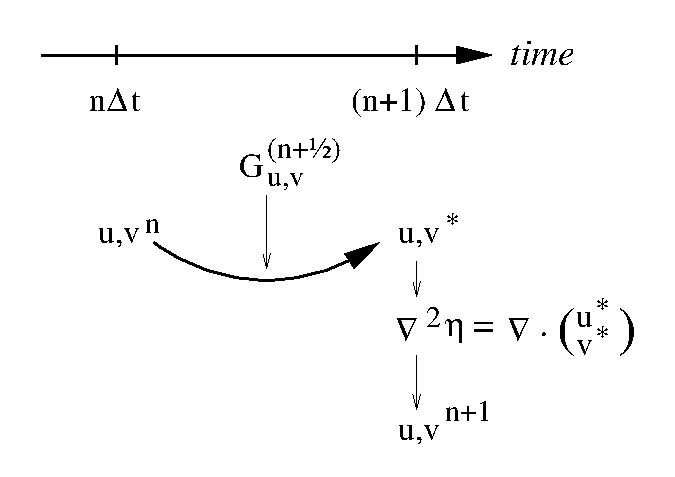
\includegraphics{part2/pressure-method-rigid-lid.eps}}
\end{center}
\caption{
A schematic of the evolution in time of the pressure method
algorithm. A prediction for the flow variables at time level $n+1$ is
made based only on the explicit terms, $G^{(n+^1/_2)}$, and denoted
$u^*$, $v^*$. Next, a pressure field is found such that $u^{n+1}$,
$v^{n+1}$ will be non-divergent. Conceptually, the $*$ quantities
exist at time level $n+1$ but they are intermediate and only
temporary.}
\label{fig:pressure-method-rigid-lid}
\end{figure}

\begin{figure}
\begin{center} \fbox{ \begin{minipage}{4.5in} \begin{tabbing}
aaa \= aaa \= aaa \= aaa \= aaa \= aaa \kill 
\filelink{FORWARD\_STEP}{model-src-forward_step.F} \\
\> DYNAMICS \\
\>\> TIMESTEP \` $u^*$,$v^*$ (\ref{eq:ustar-rigid-lid},\ref{eq:vstar-rigid-lid}) \\
\> SOLVE\_FOR\_PRESSURE \\
\>\> CALC\_DIV\_GHAT \` $H\widehat{u^*}$,$H\widehat{v^*}$ (\ref{eq:elliptic}) \\
\>\> CG2D \` $\eta^{n+1}$ (\ref{eq:elliptic}) \\
\> MOMENTUM\_CORRECTION\_STEP  \\
\>\> CALC\_GRAD\_PHI\_SURF \` $\nabla \eta^{n+1}$ \\
\>\> CORRECTION\_STEP \` $u^{n+1}$,$v^{n+1}$ (\ref{eq:un+1-rigid-lid},\ref{eq:vn+1-rigid-lid})
\end{tabbing} \end{minipage} } \end{center}
\caption{Calling tree for the pressure method algorithm 
  (\filelink{FORWARD\_STEP}{model-src-forward_step.F})}
\label{fig:call-tree-pressure-method}
\end{figure}

The horizontal momentum and continuity equations for the ocean
(\ref{eq:ocean-mom} and \ref{eq:ocean-cont}), or for the atmosphere
(\ref{eq:atmos-mom} and \ref{eq:atmos-cont}), can be summarized by:
\begin{eqnarray}
\partial_t u + g \partial_x \eta & = & G_u \\
\partial_t v + g \partial_y \eta & = & G_v \\
\partial_x u + \partial_y v + \partial_z w & = & 0
\end{eqnarray}
where we are adopting the oceanic notation for brevity. All terms in
the momentum equations, except for surface pressure gradient, are
encapsulated in the $G$ vector. The continuity equation, when
integrated over the fluid depth, $H$, and with the rigid-lid/no normal
flow boundary conditions applied, becomes:
\begin{equation}
\partial_x H \widehat{u} + \partial_y H \widehat{v} = 0
\label{eq:rigid-lid-continuity}
\end{equation}
Here, $H\widehat{u} = \int_H u dz$ is the depth integral of $u$,
similarly for $H\widehat{v}$. The rigid-lid approximation sets $w=0$
at the lid so that it does not move but allows a pressure to be
exerted on the fluid by the lid. The horizontal momentum equations and
vertically integrated continuity equation are be discretized in time
and space as follows:
\begin{eqnarray}
u^{n+1} + \Delta t g \partial_x \eta^{n+1}
& = & u^{n} + \Delta t G_u^{(n+1/2)}
\label{eq:discrete-time-u}
\\
v^{n+1} + \Delta t g \partial_y \eta^{n+1}
& = & v^{n} + \Delta t G_v^{(n+1/2)}
\label{eq:discrete-time-v}
\\
  \partial_x H \widehat{u^{n+1}}
+ \partial_y H \widehat{v^{n+1}} & = & 0
\label{eq:discrete-time-cont-rigid-lid}
\end{eqnarray}
As written here, terms on the LHS all involve time level $n+1$ and are
referred to as implicit; the implicit backward time stepping scheme is
being used. All other terms in the RHS are explicit in time. The
thermodynamic quantities are integrated forward in time in parallel
with the flow and will be discussed later. For the purposes of
describing the pressure method it suffices to say that the hydrostatic
pressure gradient is explicit and so can be included in the vector
$G$.

Substituting the two momentum equations into the depth integrated
continuity equation eliminates $u^{n+1}$ and $v^{n+1}$ yielding an
elliptic equation for $\eta^{n+1}$. Equations
\ref{eq:discrete-time-u}, \ref{eq:discrete-time-v} and
\ref{eq:discrete-time-cont-rigid-lid} can then be re-arranged as follows:
\begin{eqnarray}
u^{*} & = & u^{n} + \Delta t G_u^{(n+1/2)} \label{eq:ustar-rigid-lid} \\
v^{*} & = & v^{n} + \Delta t G_v^{(n+1/2)} \label{eq:vstar-rigid-lid} \\
  \partial_x \Delta t g H \partial_x \eta^{n+1}
+ \partial_y \Delta t g H \partial_y \eta^{n+1}
& = &
  \partial_x H \widehat{u^{*}}
+ \partial_y H \widehat{v^{*}} \label{eq:elliptic}
\\
u^{n+1} & = & u^{*} - \Delta t g \partial_x \eta^{n+1} \label{eq:un+1-rigid-lid}\\
v^{n+1} & = & v^{*} - \Delta t g \partial_y \eta^{n+1} \label{eq:vn+1-rigid-lid}
\end{eqnarray}
Equations \ref{eq:ustar-rigid-lid} to \ref{eq:vn+1-rigid-lid}, solved
sequentially, represent the pressure method algorithm used in the
model. The essence of the pressure method lies in the fact that any
explicit prediction for the flow would lead to a divergence flow field
so a pressure field must be found that keeps the flow non-divergent
over each step of the integration. The particular location in time of
the pressure field is somewhat ambiguous; in
Fig.~\ref{fig:pressure-method-rigid-lid} we depicted as co-located
with the future flow field (time level $n+1$) but it could equally
have been drawn as staggered in time with the flow.

The correspondence to the code is as follows:
\begin{itemize}
\item
the prognostic phase, equations \ref{eq:ustar-rigid-lid} and \ref{eq:vstar-rigid-lid},
stepping forward $u^n$ and $v^n$ to $u^{*}$ and $v^{*}$ is coded in
\filelink{TIMESTEP()}{model-src-timestep.F}
\item
the vertical integration, $H \widehat{u^*}$ and $H
\widehat{v^*}$, divergence and inversion of the elliptic operator in
equation \ref{eq:elliptic} is coded in 
\filelink{SOLVE\_FOR\_PRESSURE()}{model-src-solve_for_pressure.F}
\item
finally, the new flow field at time level $n+1$ given by equations
\ref{eq:un+1-rigid-lid} and \ref{eq:vn+1-rigid-lid} is calculated in 
\filelink{CORRECTION\_STEP()}{model-src-correction_step.F}.
\end{itemize}
The calling tree for these routines is given in
Fig.~\ref{fig:call-tree-pressure-method}.



\paragraph{Need to discuss implicit viscosity somewhere:}
\begin{eqnarray}
\frac{1}{\Delta t} u^{n+1} - \partial_z A_v \partial_z u^{n+1}
+ g \partial_x \eta^{n+1} & = & \frac{1}{\Delta t} u^{n} +
G_u^{(n+1/2)}
\\
\frac{1}{\Delta t} v^{n+1} - \partial_z A_v \partial_z v^{n+1}
+ g \partial_y \eta^{n+1} & = & \frac{1}{\Delta t} v^{n} + G_v^{(n+1/2)}
\end{eqnarray}


\section{Pressure method with implicit linear free-surface}
\label{sect:pressure-method-linear-backward}
\begin{rawhtml}
<!-- CMIREDIR:pressure_method_linear_backward: -->
\end{rawhtml}

The rigid-lid approximation filters out external gravity waves
subsequently modifying the dispersion relation of barotropic Rossby
waves. The discrete form of the elliptic equation has some zero
eigen-values which makes it a potentially tricky or inefficient
problem to solve.

The rigid-lid approximation can be easily replaced by a linearization
of the free-surface equation which can be written:
\begin{equation}
\partial_t \eta + \partial_x H \widehat{u} + \partial_y H \widehat{v} = P-E+R
\label{eq:linear-free-surface=P-E}
\end{equation}
which differs from the depth integrated continuity equation with
rigid-lid (\ref{eq:rigid-lid-continuity}) by the time-dependent term
and fresh-water source term.

Equation \ref{eq:discrete-time-cont-rigid-lid} in the rigid-lid
pressure method is then replaced by the time discretization of
\ref{eq:linear-free-surface=P-E} which is:
\begin{equation}
\eta^{n+1}
+ \Delta t \partial_x H \widehat{u^{n+1}}
+ \Delta t \partial_y H \widehat{v^{n+1}}
=
\eta^{n}
+ \Delta t ( P - E )
\label{eq:discrete-time-backward-free-surface}
\end{equation}
where the use of flow at time level $n+1$ makes the method implicit
and backward in time. The is the preferred scheme since it still
filters the fast unresolved wave motions by damping them. A centered
scheme, such as Crank-Nicholson, would alias the energy of the fast
modes onto slower modes of motion.

As for the rigid-lid pressure method, equations
\ref{eq:discrete-time-u}, \ref{eq:discrete-time-v} and
\ref{eq:discrete-time-backward-free-surface} can be re-arranged as follows:
\begin{eqnarray}
u^{*} & = & u^{n} + \Delta t G_u^{(n+1/2)} \label{eq:ustar-backward-free-surface} \\
v^{*} & = & v^{n} + \Delta t G_v^{(n+1/2)} \label{eq:vstar-backward-free-surface} \\
\eta^* & = & \epsilon_{fs} \left( \eta^{n} + \Delta t (P-E) \right)- \Delta t 
  \partial_x H \widehat{u^{*}}
+ \partial_y H \widehat{v^{*}}
\\
  \partial_x g H \partial_x \eta^{n+1}
& + & \partial_y g H \partial_y \eta^{n+1}
 - \frac{\epsilon_{fs} \eta^{n+1}}{\Delta t^2}
 = 
- \frac{\eta^*}{\Delta t^2}
\label{eq:elliptic-backward-free-surface}
\\
u^{n+1} & = & u^{*} - \Delta t g \partial_x \eta^{n+1} \label{eq:un+1-backward-free-surface}\\
v^{n+1} & = & v^{*} - \Delta t g \partial_y \eta^{n+1} \label{eq:vn+1-backward-free-surface}
\end{eqnarray}
Equations~\ref{eq:ustar-backward-free-surface}
to~\ref{eq:vn+1-backward-free-surface}, solved sequentially, represent
the pressure method algorithm with a backward implicit, linearized
free surface. The method is still formerly a pressure method because
in the limit of large $\Delta t$ the rigid-lid method is
recovered. However, the implicit treatment of the free-surface allows
the flow to be divergent and for the surface pressure/elevation to
respond on a finite time-scale (as opposed to instantly). To recover
the rigid-lid formulation, we introduced a switch-like parameter,
$\epsilon_{fs}$, which selects between the free-surface and rigid-lid;
$\epsilon_{fs}=1$ allows the free-surface to evolve; $\epsilon_{fs}=0$
imposes the rigid-lid. The evolution in time and location of variables
is exactly as it was for the rigid-lid model so that
Fig.~\ref{fig:pressure-method-rigid-lid} is still
applicable. Similarly, the calling sequence, given in
Fig.~\ref{fig:call-tree-pressure-method}, is as for the
pressure-method.


\section{Explicit time-stepping: Adams-Bashforth}
\label{sect:adams-bashforth}
\begin{rawhtml}
<!-- CMIREDIR:adams_bashforth: -->
\end{rawhtml}

In describing the the pressure method above we deferred describing the
time discretization of the explicit terms. We have historically used
the quasi-second order Adams-Bashforth method for all explicit terms
in both the momentum and tracer equations. This is still the default
mode of operation but it is now possible to use alternate schemes for
tracers (see section \ref{sect:tracer-advection}).

\begin{figure}
\begin{center} \fbox{ \begin{minipage}{4.5in} \begin{tabbing}
aaa \= aaa \= aaa \= aaa \= aaa \= aaa \kill 
FORWARD\_STEP \\
\> THERMODYNAMICS \\
\>\> CALC\_GT \\
\>\>\> GAD\_CALC\_RHS \` $G_\theta^n = G_\theta( u, \theta^n )$ \\
\>either\>\> EXTERNAL\_FORCING \` $G_\theta^n = G_\theta^n + {\cal Q}$ \\
\>\>\> ADAMS\_BASHFORTH2 \` $G_\theta^{(n+1/2)}$ (\ref{eq:adams-bashforth2}) \\
\>or\>\> EXTERNAL\_FORCING \` $G_\theta^{(n+1/2)} = G_\theta^{(n+1/2)} + {\cal Q}$ \\
\>\> TIMESTEP\_TRACER \` $\tau^*$ (\ref{eq:taustar}) \\
\>\> IMPLDIFF \` $\tau^{(n+1)}$ (\ref{eq:tau-n+1-implicit})
\end{tabbing} \end{minipage} } \end{center}
\caption{
Calling tree for the Adams-Bashforth time-stepping of temperature with
implicit diffusion.}
\label{fig:call-tree-adams-bashforth}
\end{figure}

In the previous sections, we summarized an explicit scheme as:
\begin{equation}
\tau^{*} = \tau^{n} + \Delta t G_\tau^{(n+1/2)}
\label{eq:taustar}
\end{equation}
where $\tau$ could be any prognostic variable ($u$, $v$, $\theta$ or
$S$) and $\tau^*$ is an explicit estimate of $\tau^{n+1}$ and would be
exact if not for implicit-in-time terms. The parenthesis about $n+1/2$
indicates that the term is explicit and extrapolated forward in time
and for this we use the quasi-second order Adams-Bashforth method:
\begin{equation}
G_\tau^{(n+1/2)} = ( 3/2 + \epsilon_{AB}) G_\tau^n
- ( 1/2 + \epsilon_{AB}) G_\tau^{n-1}
\label{eq:adams-bashforth2}
\end{equation}
This is a linear extrapolation, forward in time, to
$t=(n+1/2+{\epsilon_{AB}})\Delta t$. An extrapolation to the mid-point
in time, $t=(n+1/2)\Delta t$, corresponding to $\epsilon_{AB}=0$,
would be second order accurate but is weakly unstable for oscillatory
terms. A small but finite value for $\epsilon_{AB}$ stabilizes the
method. Strictly speaking, damping terms such as diffusion and
dissipation, and fixed terms (forcing), do not need to be inside the
Adams-Bashforth extrapolation. However, in the current code, it is
simpler to include these terms and this can be justified if the flow
and forcing evolves smoothly. Problems can, and do, arise when forcing
or motions are high frequency and this corresponds to a reduced
stability compared to a simple forward time-stepping of such terms.
The model offers the possibility to leave the forcing term outside the 
Adams-Bashforth extrapolation, by turning off the logical flag 
{\bf forcing\_In\_AB } (parameter file {\em data}, namelist {\em PARM01}, 
default value = True).

A stability analysis for an oscillation equation should be given at this point.
\marginpar{AJA needs to find his notes on this...}

A stability analysis for a relaxation equation should be given at this point.
\marginpar{...and for this too.}


\section{Implicit time-stepping: backward method}
\begin{rawhtml}
<!-- CMIREDIR:implicit_time-stepping_backward: -->
\end{rawhtml}

Vertical diffusion and viscosity can be treated implicitly in time
using the backward method which is an intrinsic scheme. 
Recently, the option to treat the vertical advection 
implicitly has been added, but not yet tested; therefore, 
the description hereafter is limited to diffusion and viscosity.
For tracers,
the time discretized equation is:
\begin{equation}
\tau^{n+1} - \Delta t \partial_r \kappa_v \partial_r \tau^{n+1} =
\tau^{n} + \Delta t G_\tau^{(n+1/2)}
\label{eq:implicit-diffusion}
\end{equation}
where $G_\tau^{(n+1/2)}$ is the remaining explicit terms extrapolated
using the Adams-Bashforth method as described above.  Equation
\ref{eq:implicit-diffusion} can be split split into:
\begin{eqnarray}
\tau^* & = & \tau^{n} + \Delta t G_\tau^{(n+1/2)}
\label{eq:taustar-implicit} \\
\tau^{n+1} & = & {\cal L}_\tau^{-1} ( \tau^* )
\label{eq:tau-n+1-implicit}
\end{eqnarray}
where ${\cal L}_\tau^{-1}$ is the inverse of the operator
\begin{equation}
{\cal L} = \left[ 1 + \Delta t \partial_r \kappa_v \partial_r \right]
\end{equation}
Equation \ref{eq:taustar-implicit} looks exactly as \ref{eq:taustar}
while \ref{eq:tau-n+1-implicit} involves an operator or matrix
inversion. By re-arranging \ref{eq:implicit-diffusion} in this way we
have cast the method as an explicit prediction step and an implicit
step allowing the latter to be inserted into the over all algorithm
with minimal interference.

Fig.~\ref{fig:call-tree-adams-bashforth} shows the calling sequence for
stepping forward a tracer variable such as temperature.

In order to fit within the pressure method, the implicit viscosity
must not alter the barotropic flow. In other words, it can only
redistribute momentum in the vertical. The upshot of this is that
although vertical viscosity may be backward implicit and
unconditionally stable, no-slip boundary conditions may not be made
implicit and are thus cast as a an explicit drag term.

\section{Synchronous time-stepping: variables co-located in time}
\label{sect:adams-bashforth-sync}
\begin{rawhtml}
<!-- CMIREDIR:adams_bashforth_sync: -->
\end{rawhtml}

\begin{figure}
\begin{center}
\resizebox{5.0in}{!}{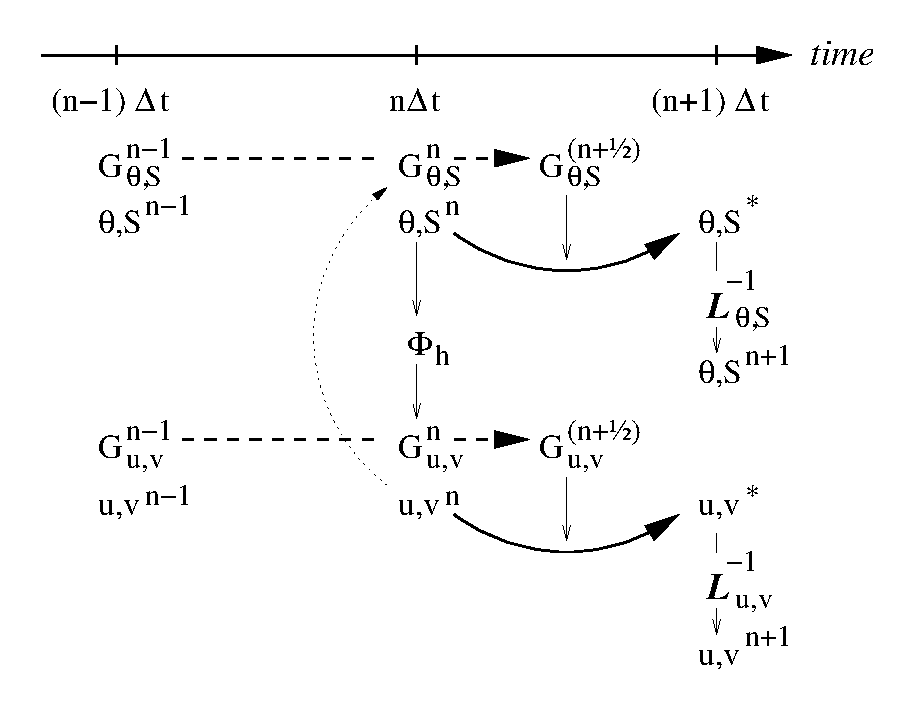
\includegraphics{part2/adams-bashforth-sync.eps}}
\end{center}
\caption{
A schematic of the explicit Adams-Bashforth and implicit time-stepping
phases of the algorithm. All prognostic variables are co-located in
time. Explicit tendencies are evaluated at time level $n$ as a
function of the state at that time level (dotted arrow). The explicit
tendency from the previous time level, $n-1$, is used to extrapolate
tendencies to $n+1/2$ (dashed arrow). This extrapolated tendency
allows variables to be stably integrated forward-in-time to render an
estimate ($*$-variables) at the $n+1$ time level (solid
arc-arrow). The operator ${\cal L}$ formed from implicit-in-time terms
is solved to yield the state variables at time level $n+1$. }
\label{fig:adams-bashforth-sync}
\end{figure}

\begin{figure}
\begin{center} \fbox{ \begin{minipage}{4.7in} \begin{tabbing}
aaa \= aaa \= aaa \= aaa \= aaa \= aaa \kill 
FORWARD\_STEP \\
\>\> EXTERNAL\_FIELDS\_LOAD\\
\>\> DO\_ATMOSPHERIC\_PHYS \\
\>\> DO\_OCEANIC\_PHYS \\
\> THERMODYNAMICS \\
\>\> CALC\_GT \\
\>\>\> GAD\_CALC\_RHS \` $G_\theta^n = G_\theta( u, \theta^n )$ (\ref{eq:Gt-n-sync})\\
\>\>\> EXTERNAL\_FORCING \` $G_\theta^n = G_\theta^n + {\cal Q}$ \\
\>\>\> ADAMS\_BASHFORTH2 \` $G_\theta^{(n+1/2)}$ (\ref{eq:Gt-n+5-sync}) \\
\>\> TIMESTEP\_TRACER \` $\theta^*$ (\ref{eq:tstar-sync}) \\
\>\> IMPLDIFF \` $\theta^{(n+1)}$ (\ref{eq:t-n+1-sync}) \\
\> DYNAMICS \\
\>\> CALC\_PHI\_HYD \` $\phi_{hyd}^n$ (\ref{eq:phi-hyd-sync}) \\
\>\> MOM\_FLUXFORM or MOM\_VECINV \` $G_{\vec{\bf v}}^n$ (\ref{eq:Gv-n-sync})\\
\>\> TIMESTEP \` $\vec{\bf v}^*$ (\ref{eq:Gv-n+5-sync}, \ref{eq:vstar-sync}) \\
\>\> IMPLDIFF \` $\vec{\bf v}^{**}$ (\ref{eq:vstarstar-sync}) \\
\> UPDATE\_R\_STAR or UPDATE\_SURF\_DR \` (NonLin-FS only)\\
\> SOLVE\_FOR\_PRESSURE \\
\>\> CALC\_DIV\_GHAT \` $\eta^*$ (\ref{eq:nstar-sync}) \\
\>\> CG2D \` $\eta^{n+1}$ (\ref{eq:elliptic-sync}) \\
\> MOMENTUM\_CORRECTION\_STEP  \\
\>\> CALC\_GRAD\_PHI\_SURF \` $\nabla \eta^{n+1}$ \\
\>\> CORRECTION\_STEP \` $u^{n+1}$,$v^{n+1}$ (\ref{eq:v-n+1-sync})\\
\> TRACERS\_CORRECTION\_STEP  \\
\>\> CYCLE\_TRACER \` $\theta^{n+1}$ \\
\>\> FILTER \` Shapiro Filter, Zonal Filter (FFT) \\
\>\> CONVECTIVE\_ADJUSTMENT \` \\
\end{tabbing} \end{minipage} } \end{center}
\caption{
Calling tree for the overall synchronous algorithm using
Adams-Bashforth time-stepping. 
The place where the model geometry
({\bf hFac} factors) is updated is added here but is only relevant 
for the non-linear free-surface algorithm.
For completeness, the external forcing,
ocean and atmospheric physics have been added, although they are mainly 
optional}
\label{fig:call-tree-adams-bashforth-sync}
\end{figure}

The Adams-Bashforth extrapolation of explicit tendencies fits neatly
into the pressure method algorithm when all state variables are
co-located in time. Fig.~\ref{fig:adams-bashforth-sync} illustrates
the location of variables in time and the evolution of the algorithm
with time. The algorithm can be represented by the sequential solution
of the follow equations:
\begin{eqnarray}
G_{\theta,S}^{n} & = & G_{\theta,S} ( u^n, \theta^n, S^n )
\label{eq:Gt-n-sync} \\
G_{\theta,S}^{(n+1/2)} & = & (3/2+\epsilon_{AB}) G_{\theta,S}^{n}-(1/2+\epsilon_{AB}) G_{\theta,S}^{n-1}
\label{eq:Gt-n+5-sync} \\
(\theta^*,S^*) & = & (\theta^{n},S^{n}) + \Delta t G_{\theta,S}^{(n+1/2)}
\label{eq:tstar-sync} \\
(\theta^{n+1},S^{n+1}) & = & {\cal L}^{-1}_{\theta,S} (\theta^*,S^*)
\label{eq:t-n+1-sync} \\
\phi^n_{hyd} & = & \int b(\theta^n,S^n) dr
\label{eq:phi-hyd-sync} \\
\vec{\bf G}_{\vec{\bf v}}^{n} & = & \vec{\bf G}_{\vec{\bf v}} ( \vec{\bf v}^n, \phi^n_{hyd} )
\label{eq:Gv-n-sync} \\
\vec{\bf G}_{\vec{\bf v}}^{(n+1/2)} & = & (3/2 + \epsilon_{AB} ) \vec{\bf G}_{\vec{\bf v}}^{n} - (1/2 + \epsilon_{AB} ) \vec{\bf G}_{\vec{\bf v}}^{n-1}
\label{eq:Gv-n+5-sync} \\
\vec{\bf v}^{*} & = & \vec{\bf v}^{n} + \Delta t \vec{\bf G}_{\vec{\bf v}}^{(n+1/2)}
\label{eq:vstar-sync} \\
\vec{\bf v}^{**} & = & {\cal L}_{\vec{\bf v}}^{-1} ( \vec{\bf v}^* )
\label{eq:vstarstar-sync} \\
\eta^* & = & \epsilon_{fs} \left( \eta^{n} + \Delta t (P-E) \right)- \Delta t 
  \nabla \cdot H \widehat{ \vec{\bf v}^{**} }
\label{eq:nstar-sync} \\
\nabla \cdot g H \nabla \eta^{n+1} & - & \frac{\epsilon_{fs} \eta^{n+1}}{\Delta t^2}
~ = ~ - \frac{\eta^*}{\Delta t^2}
\label{eq:elliptic-sync} \\
\vec{\bf v}^{n+1} & = & \vec{\bf v}^{*} - \Delta t g \nabla \eta^{n+1}
\label{eq:v-n+1-sync}
\end{eqnarray}
Fig.~\ref{fig:adams-bashforth-sync} illustrates the location of
variables in time and evolution of the algorithm with time. The
Adams-Bashforth extrapolation of the tracer tendencies is illustrated
by the dashed arrow, the prediction at $n+1$ is indicated by the
solid arc. Inversion of the implicit terms, ${\cal
L}^{-1}_{\theta,S}$, then yields the new tracer fields at $n+1$. All
these operations are carried out in subroutine {\em THERMODYNAMICS} an
subsidiaries, which correspond to equations \ref{eq:Gt-n-sync} to
\ref{eq:t-n+1-sync}.
Similarly illustrated is the Adams-Bashforth extrapolation of
accelerations, stepping forward and solving of implicit viscosity and
surface pressure gradient terms, corresponding to equations
\ref{eq:Gv-n-sync} to \ref{eq:v-n+1-sync}.
These operations are carried out in subroutines {\em DYNAMCIS}, {\em
SOLVE\_FOR\_PRESSURE} and {\em MOMENTUM\_CORRECTION\_STEP}. This, then,
represents an entire algorithm for stepping forward the model one
time-step. The corresponding calling tree is given in
\ref{fig:call-tree-adams-bashforth-sync}.

\section{Staggered baroclinic time-stepping}
\label{sect:adams-bashforth-staggered}
\begin{rawhtml}
<!-- CMIREDIR:adams_bashforth_staggered: -->
\end{rawhtml}

\begin{figure}
\begin{center}
\resizebox{5.5in}{!}{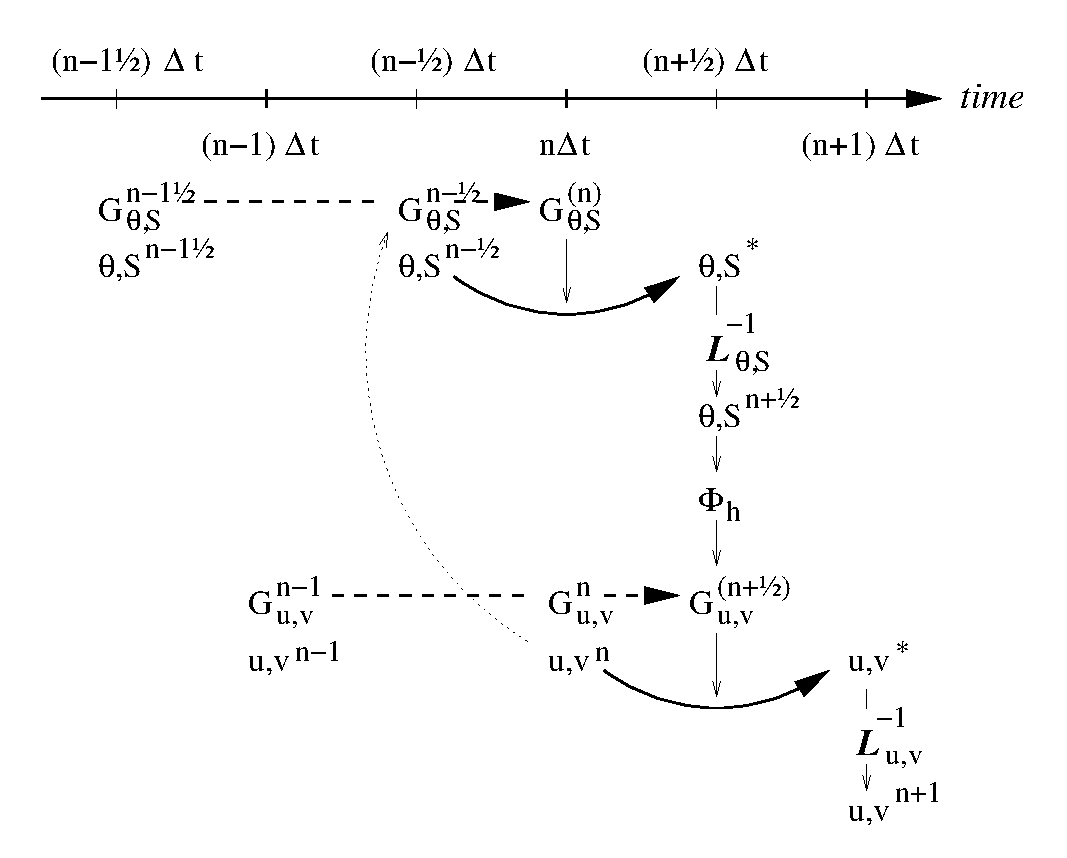
\includegraphics{part2/adams-bashforth-staggered.eps}}
\end{center}
\caption{
A schematic of the explicit Adams-Bashforth and implicit time-stepping
phases of the algorithm but with staggering in time of thermodynamic
variables with the flow. 
Explicit momentum tendencies are evaluated at time level $n-1/2$ as a 
function of the flow field at that time level $n-1/2$.
The explicit tendency from the previous time level, $n-3/2$, is used to
extrapolate tendencies to $n$ (dashed arrow). 
The hydrostatic pressure/geo-potential $\phi_{hyd}$ is evaluated directly 
at time level $n$ (vertical arrows) and used with the extrapolated tendencies
to step forward the flow variables from $n-1/2$ to $n+1/2$ (solid arc-arrow).
The implicit-in-time operator ${\cal L}_{\bf u,v}$ (vertical arrows) is 
then applied to the previous estimation of the the flow field ($*$-variables) 
and yields to the two velocity components $u,v$ at time level $n+1/2$. 
These are then used to calculate the advection term (dashed arc-arrow) 
of the thermo-dynamics tendencies at time step $n$.
The extrapolated thermodynamics tendency, from time level $n-1$ and $n$ 
to $n+1/2$, allows thermodynamic variables to be stably integrated 
forward-in-time (solid arc-arrow) up to time level $n+1$.
}
\label{fig:adams-bashforth-staggered}
\end{figure}

For well stratified problems, internal gravity waves may be the
limiting process for determining a stable time-step. In the
circumstance, it is more efficient to stagger in time the
thermodynamic variables with the flow
variables. Fig.~\ref{fig:adams-bashforth-staggered} illustrates the
staggering and algorithm. The key difference between this and
Fig.~\ref{fig:adams-bashforth-sync} is that the thermodynamic variables 
are solved after the dynamics, using the recently updated flow field.
This essentially allows the gravity wave terms to leap-frog in
time giving second order accuracy and more stability.

The essential change in the staggered algorithm is that the 
thermodynamics solver is delayed from half a time step, 
allowing the use of the most recent velocities to compute 
the advection terms. Once the thermodynamics fields are
updated, the hydrostatic pressure is computed 
to step forwrad the dynamics.
Note that the pressure gradient must also be taken out of the
Adams-Bashforth extrapolation. Also, retaining the integer time-levels,
$n$ and $n+1$, does not give a user the sense of where variables are
located in time.  Instead, we re-write the entire algorithm,
\ref{eq:Gt-n-sync} to \ref{eq:v-n+1-sync}, annotating the
position in time of variables appropriately:
\begin{eqnarray}
\phi^{n}_{hyd} & = & \int b(\theta^{n},S^{n}) dr
\label{eq:phi-hyd-staggered} \\
\vec{\bf G}_{\vec{\bf v}}^{n-1/2} & = & \vec{\bf G}_{\vec{\bf v}} ( \vec{\bf v}^{n-1/2} )
\label{eq:Gv-n-staggered} \\
\vec{\bf G}_{\vec{\bf v}}^{(n)} & = & (3/2 + \epsilon_{AB} ) \vec{\bf G}_{\vec{\bf v}}^{n-1/2} - (1/2 + \epsilon_{AB} ) \vec{\bf G}_{\vec{\bf v}}^{n-3/2}
\label{eq:Gv-n+5-staggered} \\
\vec{\bf v}^{*} & = & \vec{\bf v}^{n-1/2} + \Delta t \left( \vec{\bf G}_{\vec{\bf v}}^{(n)} - \nabla \phi_{hyd}^{n} \right)
\label{eq:vstar-staggered} \\
\vec{\bf v}^{**} & = & {\cal L}_{\vec{\bf v}}^{-1} ( \vec{\bf v}^* )
\label{eq:vstarstar-staggered} \\
\eta^* & = & \epsilon_{fs} \left( \eta^{n-1/2} + \Delta t (P-E)^n \right)- \Delta t 
  \nabla \cdot H \widehat{ \vec{\bf v}^{**} }
\label{eq:nstar-staggered} \\
\nabla \cdot g H \nabla \eta^{n+1/2} & - & \frac{\epsilon_{fs} \eta^{n+1/2}}{\Delta t^2}
~ = ~ - \frac{\eta^*}{\Delta t^2}
\label{eq:elliptic-staggered} \\
\vec{\bf v}^{n+1/2} & = & \vec{\bf v}^{*} - \Delta t g \nabla \eta^{n+1/2}
\label{eq:v-n+1-staggered} \\
G_{\theta,S}^{n} & = & G_{\theta,S} ( u^{n+1/2}, \theta^{n}, S^{n} )
\label{eq:Gt-n-staggered} \\
G_{\theta,S}^{(n+1/2)} & = & (3/2+\epsilon_{AB}) G_{\theta,S}^{n}-(1/2+\epsilon_{AB}) G_{\theta,S}^{n-1}
\label{eq:Gt-n+5-staggered} \\
(\theta^*,S^*) & = & (\theta^{n},S^{n}) + \Delta t G_{\theta,S}^{(n+1/2)}
\label{eq:tstar-staggered} \\
(\theta^{n+1},S^{n+1}) & = & {\cal L}^{-1}_{\theta,S} (\theta^*,S^*)
\label{eq:t-n+1-staggered}
\end{eqnarray}
The corresponding calling tree is given in
\ref{fig:call-tree-adams-bashforth-staggered}.
The staggered algorithm is activated with the run-time flag 
{\bf staggerTimeStep}{\em=.TRUE.} in parameter file {\em data},
namelist {\em PARM01}.

\begin{figure}
\begin{center} \fbox{ \begin{minipage}{4.7in} \begin{tabbing}
aaa \= aaa \= aaa \= aaa \= aaa \= aaa \kill 
FORWARD\_STEP \\
\>\> EXTERNAL\_FIELDS\_LOAD\\
\>\> DO\_ATMOSPHERIC\_PHYS \\
\>\> DO\_OCEANIC\_PHYS \\
\> DYNAMICS \\
\>\> CALC\_PHI\_HYD \` $\phi_{hyd}^n$ (\ref{eq:phi-hyd-staggered}) \\
\>\> MOM\_FLUXFORM or MOM\_VECINV \` $G_{\vec{\bf v}}^{n-1/2}$ 
    (\ref{eq:Gv-n-staggered})\\
\>\> TIMESTEP \` $\vec{\bf v}^*$ (\ref{eq:Gv-n+5-staggered}, 
                                  \ref{eq:vstar-staggered}) \\
\>\> IMPLDIFF \` $\vec{\bf v}^{**}$ (\ref{eq:vstarstar-staggered}) \\
\> UPDATE\_R\_STAR or UPDATE\_SURF\_DR \` (NonLin-FS only)\\
\> SOLVE\_FOR\_PRESSURE \\
\>\> CALC\_DIV\_GHAT \` $\eta^*$ (\ref{eq:nstar-staggered}) \\
\>\> CG2D \` $\eta^{n+1/2}$ (\ref{eq:elliptic-staggered}) \\
\> MOMENTUM\_CORRECTION\_STEP  \\
\>\> CALC\_GRAD\_PHI\_SURF \` $\nabla \eta^{n+1/2}$ \\
\>\> CORRECTION\_STEP \` $u^{n+1/2}$,$v^{n+1/2}$ (\ref{eq:v-n+1-staggered})\\
\> THERMODYNAMICS \\
\>\> CALC\_GT \\
\>\>\> GAD\_CALC\_RHS \` $G_\theta^n = G_\theta( u, \theta^n )$ 
     (\ref{eq:Gt-n-staggered})\\
\>\>\> EXTERNAL\_FORCING \` $G_\theta^n = G_\theta^n + {\cal Q}$ \\
\>\>\> ADAMS\_BASHFORTH2 \` $G_\theta^{(n+1/2)}$ (\ref{eq:Gt-n+5-staggered}) \\
\>\> TIMESTEP\_TRACER \` $\theta^*$ (\ref{eq:tstar-staggered}) \\
\>\> IMPLDIFF \` $\theta^{(n+1)}$ (\ref{eq:t-n+1-staggered}) \\
\> TRACERS\_CORRECTION\_STEP  \\
\>\> CYCLE\_TRACER \` $\theta^{n+1}$ \\
\>\> FILTER \` Shapiro Filter, Zonal Filter (FFT) \\
\>\> CONVECTIVE\_ADJUSTMENT \` \\
\end{tabbing} \end{minipage} } \end{center}
\caption{
Calling tree for the overall staggered algorithm using
Adams-Bashforth time-stepping. 
The place where the model geometry
({\bf hFac} factors) is updated is added here but is only relevant 
for the non-linear free-surface algorithm.
}
\label{fig:call-tree-adams-bashforth-staggered}
\end{figure}

The only difficulty with this approach is apparent in equation
\ref{eq:Gt-n-staggered} and illustrated by the dotted arrow
connecting $u,v^{n+1/2}$ with $G_\theta^{n}$. The flow used to advect
tracers around is not naturally located in time. This could be avoided
by applying the Adams-Bashforth extrapolation to the tracer field
itself and advecting that around but this approach is not yet
available. We're not aware of any detrimental effect of this
feature. The difficulty lies mainly in interpretation of what
time-level variables and terms correspond to.


\section{Non-hydrostatic formulation}
\label{sect:non-hydrostatic}
\begin{rawhtml}
<!-- CMIREDIR:non-hydrostatic_formulation: -->
\end{rawhtml}

The non-hydrostatic formulation re-introduces the full vertical
momentum equation and requires the solution of a 3-D elliptic
equations for non-hydrostatic pressure perturbation. We still
intergrate vertically for the hydrostatic pressure and solve a 2-D
elliptic equation for the surface pressure/elevation for this reduces
the amount of work needed to solve for the non-hydrostatic pressure.

The momentum equations are discretized in time as follows:
\begin{eqnarray}
\frac{1}{\Delta t} u^{n+1} + g \partial_x \eta^{n+1} + \partial_x \phi_{nh}^{n+1}
& = & \frac{1}{\Delta t} u^{n} + G_u^{(n+1/2)} \label{eq:discrete-time-u-nh} \\
\frac{1}{\Delta t} v^{n+1} + g \partial_y \eta^{n+1} + \partial_y \phi_{nh}^{n+1}
& = & \frac{1}{\Delta t} v^{n} + G_v^{(n+1/2)} \label{eq:discrete-time-v-nh} \\
\frac{1}{\Delta t} w^{n+1} + \partial_r \phi_{nh}^{n+1}
& = & \frac{1}{\Delta t} w^{n} + G_w^{(n+1/2)} \label{eq:discrete-time-w-nh} \\
\end{eqnarray}
which must satisfy the discrete-in-time depth integrated continuity,
equation~\ref{eq:discrete-time-backward-free-surface} and the local continuity equation
\begin{equation}
\partial_x u^{n+1} + \partial_y v^{n+1} + \partial_r w^{n+1} = 0
\label{eq:non-divergence-nh}
\end{equation}
As before, the explicit predictions for momentum are consolidated as:
\begin{eqnarray*}
u^* & = & u^n + \Delta t G_u^{(n+1/2)} \\
v^* & = & v^n + \Delta t G_v^{(n+1/2)} \\
w^* & = & w^n + \Delta t G_w^{(n+1/2)}
\end{eqnarray*}
but this time we introduce an intermediate step by splitting the
tendancy of the flow as follows:
\begin{eqnarray}
u^{n+1} = u^{**} - \Delta t \partial_x \phi_{nh}^{n+1}
& &
u^{**} = u^{*} - \Delta t g \partial_x \eta^{n+1} \\
v^{n+1} = v^{**} - \Delta t \partial_y \phi_{nh}^{n+1}
& &
v^{**} = v^{*} - \Delta t g \partial_y \eta^{n+1}
\end{eqnarray}
Substituting into the depth integrated continuity
(equation~\ref{eq:discrete-time-backward-free-surface}) gives
\begin{equation}
\partial_x H \partial_x \left( g \eta^{n+1} + \widehat{\phi}_{nh}^{n+1} \right)
+
\partial_y H \partial_y \left( g \eta^{n+1} + \widehat{\phi}_{nh}^{n+1} \right)
 - \frac{\epsilon_{fs}\eta^*}{\Delta t^2}
= - \frac{\eta^*}{\Delta t^2}
\end{equation}
which is approximated by equation
\ref{eq:elliptic-backward-free-surface} on the basis that i)
$\phi_{nh}^{n+1}$ is not yet known and ii) $\nabla \widehat{\phi}_{nh}
<< g \nabla \eta$. If \ref{eq:elliptic-backward-free-surface} is
solved accurately then the implication is that $\widehat{\phi}_{nh}
\approx 0$ so that thet non-hydrostatic pressure field does not drive
barotropic motion.

The flow must satisfy non-divergence
(equation~\ref{eq:non-divergence-nh}) locally, as well as depth
integrated, and this constraint is used to form a 3-D elliptic
equations for $\phi_{nh}^{n+1}$:
\begin{equation}
\partial_{xx} \phi_{nh}^{n+1} + \partial_{yy} \phi_{nh}^{n+1} + 
\partial_{rr} \phi_{nh}^{n+1} =
\partial_x u^{**} + \partial_y v^{**} + \partial_r w^{*}
\end{equation}

The entire algorithm can be summarized as the sequential solution of
the following equations:
\begin{eqnarray}
u^{*} & = & u^{n} + \Delta t G_u^{(n+1/2)} \label{eq:ustar-nh} \\
v^{*} & = & v^{n} + \Delta t G_v^{(n+1/2)} \label{eq:vstar-nh} \\
w^{*} & = & w^{n} + \Delta t G_w^{(n+1/2)} \label{eq:wstar-nh} \\
\eta^* ~ = ~ \epsilon_{fs} \left( \eta^{n} + \Delta t (P-E) \right)
& - & \Delta t 
  \partial_x H \widehat{u^{*}}
+ \partial_y H \widehat{v^{*}}
\\
  \partial_x g H \partial_x \eta^{n+1}
+ \partial_y g H \partial_y \eta^{n+1}
& - & \frac{\epsilon_{fs} \eta^{n+1}}{\Delta t^2}
~ = ~
- \frac{\eta^*}{\Delta t^2}
\label{eq:elliptic-nh}
\\
u^{**} & = & u^{*} - \Delta t g \partial_x \eta^{n+1} \label{eq:unx-nh}\\
v^{**} & = & v^{*} - \Delta t g \partial_y \eta^{n+1} \label{eq:vnx-nh}\\
\partial_{xx} \phi_{nh}^{n+1} + \partial_{yy} \phi_{nh}^{n+1} + 
\partial_{rr} \phi_{nh}^{n+1} & = &
\partial_x u^{**} + \partial_y v^{**} + \partial_r w^{*} \\
u^{n+1} & = & u^{**} - \Delta t \partial_x \phi_{nh}^{n+1} \label{eq:un+1-nh}\\
v^{n+1} & = & v^{**} - \Delta t \partial_y \phi_{nh}^{n+1} \label{eq:vn+1-nh}\\
\partial_r w^{n+1} & = & - \partial_x u^{n+1} - \partial_y v^{n+1}
\end{eqnarray}
where the last equation is solved by vertically integrating for
$w^{n+1}$. 



\section{Variants on the Free Surface}
\label{sect:free-surface}

We now describe the various formulations of the free-surface that
include non-linear forms, implicit in time using Crank-Nicholson,
explicit and [one day] split-explicit. First, we'll reiterate the
underlying algorithm but this time using the notation consistent with
the more general vertical coordinate $r$. The elliptic equation for
free-surface coordinate (units of $r$), corresponding to
\ref{eq:discrete-time-backward-free-surface}, and
assuming no non-hydrostatic effects ($\epsilon_{nh} = 0$) is:
\begin{eqnarray}
\epsilon_{fs} {\eta}^{n+1} -
{\bf \nabla}_h \cdot \Delta t^2 (R_o-R_{fixed}) {\bf \nabla}_h b_s
{\eta}^{n+1} = {\eta}^*
\label{eq-solve2D}
\end{eqnarray}
where
\begin{eqnarray}
{\eta}^* = \epsilon_{fs} \: {\eta}^{n} -
\Delta t {\bf \nabla}_h \cdot \int_{R_{fixed}}^{R_o} \vec{\bf v}^* dr
\: + \: \epsilon_{fw} \Delta_t (P-E)^{n} 
\label{eq-solve2D_rhs}
\end{eqnarray}

\fbox{ \begin{minipage}{4.75in}
{\em S/R SOLVE\_FOR\_PRESSURE} ({\em solve\_for\_pressure.F})

$u^*$: {\bf GuNm1} ({\em DYNVARS.h})

$v^*$: {\bf GvNm1} ({\em DYNVARS.h})

$\eta^*$: {\bf cg2d\_b} (\em SOLVE\_FOR\_PRESSURE.h)

$\eta^{n+1}$: {\bf etaN} (\em DYNVARS.h)

\end{minipage} }


Once ${\eta}^{n+1}$ has been found, substituting into
\ref{eq:discrete-time-u}, \ref{eq:discrete-time-v} yields $\vec{\bf v}^{n+1}$ 
if the model is hydrostatic ($\epsilon_{nh}=0$):
$$
\vec{\bf v}^{n+1} = \vec{\bf v}^{*}
- \Delta t {\bf \nabla}_h b_s {\eta}^{n+1}
$$

This is known as the correction step. However, when the model is
non-hydrostatic ($\epsilon_{nh}=1$) we need an additional step and an
additional equation for $\phi'_{nh}$. This is obtained by substituting
\ref{eq:discrete-time-u-nh}, \ref{eq:discrete-time-v-nh} and \ref{eq:discrete-time-w-nh}
into continuity:
\begin{equation}
\left[ {\bf \nabla}_h^2 + \partial_{rr} \right] {\phi'_{nh}}^{n+1}
= \frac{1}{\Delta t} \left(
{\bf \nabla}_h \cdot \vec{\bf v}^{**} + \partial_r \dot{r}^* \right)
\end{equation}
where
\begin{displaymath}
\vec{\bf v}^{**} = \vec{\bf v}^* - \Delta t {\bf \nabla}_h b_s {\eta}^{n+1}
\end{displaymath}
Note that $\eta^{n+1}$ is also used to update the second RHS term
$\partial_r \dot{r}^* $ since
the vertical velocity at the surface ($\dot{r}_{surf}$) 
is evaluated as $(\eta^{n+1} - \eta^n) / \Delta t$.

Finally, the horizontal velocities at the new time level are found by:
\begin{equation}
\vec{\bf v}^{n+1} = \vec{\bf v}^{**}
- \epsilon_{nh} \Delta t {\bf \nabla}_h {\phi'_{nh}}^{n+1}
\end{equation}
and the vertical velocity is found by integrating the continuity
equation vertically.  Note that, for the convenience of the restart
procedure, the vertical integration of the continuity equation has
been moved to the beginning of the time step (instead of at the end),
without any consequence on the solution.

\fbox{ \begin{minipage}{4.75in}
{\em S/R CORRECTION\_STEP} ({\em correction\_step.F})

$\eta^{n+1}$: {\bf etaN} (\em DYNVARS.h)

$\phi_{nh}^{n+1}$: {\bf phi\_nh} (\em DYNVARS.h)

$u^*$: {\bf GuNm1} ({\em DYNVARS.h})

$v^*$: {\bf GvNm1} ({\em DYNVARS.h})

$u^{n+1}$: {\bf uVel} ({\em DYNVARS.h})

$v^{n+1}$: {\bf vVel} ({\em DYNVARS.h})

\end{minipage} }



Regarding the implementation of the surface pressure solver, all
computation are done within the routine {\it SOLVE\_FOR\_PRESSURE} and
its dependent calls.  The standard method to solve the 2D elliptic
problem (\ref{eq-solve2D}) uses the conjugate gradient method (routine
{\it CG2D}); the solver matrix and conjugate gradient operator are
only function of the discretized domain and are therefore evaluated
separately, before the time iteration loop, within {\it INI\_CG2D}.
The computation of the RHS $\eta^*$ is partly done in {\it
CALC\_DIV\_GHAT} and in {\it SOLVE\_FOR\_PRESSURE}.

The same method is applied for the non hydrostatic part, using a
conjugate gradient 3D solver ({\it CG3D}) that is initialized in {\it
INI\_CG3D}. The RHS terms of 2D and 3D problems are computed together
at the same point in the code.



\subsection{Crank-Nickelson barotropic time stepping}
\label{sect:freesurf-CrankNick}

The full implicit time stepping described previously is
unconditionally stable but damps the fast gravity waves, resulting in
a loss of potential energy.  The modification presented now allows one
to combine an implicit part ($\beta,\gamma$) and an explicit part
($1-\beta,1-\gamma$) for the surface pressure gradient ($\beta$) and
for the barotropic flow divergence ($\gamma$).
\\
For instance, $\beta=\gamma=1$ is the previous fully implicit scheme;
$\beta=\gamma=1/2$ is the non damping (energy conserving), unconditionally
stable, Crank-Nickelson scheme; $(\beta,\gamma)=(1,0)$ or $=(0,1)$
corresponds to the forward - backward scheme that conserves energy but is
only stable for small time steps.\\
In the code, $\beta,\gamma$ are defined as parameters, respectively 
{\bf implicSurfPress}, {\bf implicDiv2DFlow}. They are read from
the main parameter file "{\em data}" and are set by default to 1,1.

Equations \ref{eq:ustar-backward-free-surface} --
\ref{eq:vn+1-backward-free-surface} are modified as follows:
\begin{eqnarray*}
\frac{ \vec{\bf v}^{n+1} }{ \Delta t }
+ {\bf \nabla}_h b_s [ \beta {\eta}^{n+1} + (1-\beta) {\eta}^{n} ] 
+ \epsilon_{nh} {\bf \nabla}_h {\phi'_{nh}}^{n+1}
 = \frac{ \vec{\bf v}^* }{ \Delta t }
\end{eqnarray*}
\begin{eqnarray}
\epsilon_{fs} \frac{ {\eta}^{n+1} - {\eta}^{n} }{ \Delta t}
+ {\bf \nabla}_h \cdot \int_{R_{fixed}}^{R_o} 
[ \gamma \vec{\bf v}^{n+1} + (1-\gamma) \vec{\bf v}^{n}] dr
= \epsilon_{fw} (P-E)
\label{eq:eta-n+1-CrankNick}
\end{eqnarray}
where:
\begin{eqnarray*}
\vec{\bf v}^* & = &
\vec{\bf v} ^{n} + \Delta t \vec{\bf G}_{\vec{\bf v}} ^{(n+1/2)}
+ (\beta-1) \Delta t {\bf \nabla}_h b_s {\eta}^{n}
+ \Delta t {\bf \nabla}_h {\phi'_{hyd}}^{(n+1/2)}
\\
{\eta}^* & = &
\epsilon_{fs} {\eta}^{n} + \epsilon_{fw} \Delta t (P-E) 
- \Delta t {\bf \nabla}_h \cdot \int_{R_{fixed}}^{R_o} 
[ \gamma \vec{\bf v}^* + (1-\gamma) \vec{\bf v}^{n}] dr
\end{eqnarray*}
\\
In the hydrostatic case ($\epsilon_{nh}=0$), allowing us to find
${\eta}^{n+1}$, thus:
$$
\epsilon_{fs} {\eta}^{n+1} -
{\bf \nabla}_h \cdot \beta\gamma \Delta t^2 b_s (R_o - R_{fixed})
{\bf \nabla}_h {\eta}^{n+1}
= {\eta}^*
$$ 
and then to compute ({\em CORRECTION\_STEP}):
$$
\vec{\bf v}^{n+1} = \vec{\bf v}^{*}
- \beta \Delta t {\bf \nabla}_h b_s {\eta}^{n+1}
$$

%The non-hydrostatic part is solved as described previously. 

\noindent
Notes:
\begin{enumerate}
\item The RHS term of equation \ref{eq:eta-n+1-CrankNick} 
corresponds the contribution of fresh water flux (P-E) 
to the free-surface variations ($\epsilon_{fw}=1$, 
{\bf useRealFreshWater}{\em=TRUE} in parameter file {\em data}).
In order to remain consistent with the tracer equation, specially in 
the non-linear free-surface formulation, this term is also 
affected by the Crank-Nickelson time stepping. The RHS reads:
$\epsilon_{fw} ( \gamma (P-E)^{n+1/2} + (1-\gamma) (P-E)^{n-1/2} )$
\item The non-hydrostatic part of the code has not yet been 
updated, and therefore cannot be used with $(\beta,\gamma) \neq (1,1)$.
\item The stability criteria with Crank-Nickelson time stepping
for the pure linear gravity wave problem in cartesian coordinates is:
\begin{itemize}
\item $\beta + \gamma < 1$ : unstable
\item $\beta \geq 1/2$ and $ \gamma \geq 1/2$ : stable
\item $\beta + \gamma \geq 1$ : stable if
$$ 
c_{max}^2 (\beta - 1/2)(\gamma - 1/2) + 1 \geq 0
$$
$$
\mbox{with }~
%c^2 = 2 g H {\Delta t}^2 
%(\frac{1-cos 2 \pi / k}{\Delta x^2} 
%+\frac{1-cos 2 \pi / l}{\Delta y^2})
%$$
%Practically, the most stringent condition is obtained with $k=l=2$ :
%$$
c_{max} =  2 \Delta t \: \sqrt{g H} \: 
\sqrt{ \frac{1}{\Delta x^2} + \frac{1}{\Delta y^2} }
$$
\end{itemize}
\end{enumerate}


% $Header: /u/gcmpack/manual/s_algorithm/text/nonlin_frsurf.tex,v 1.6 2001/11/13 20:13:54 adcroft Exp $
% $Name:  $



\subsection{Non-linear free surface}
\label{sect:nonlinear-freesurface}

Recently, two options have been added to the model (and have not yet
been extensively tested) that concern the free surface formulation.


\subsubsection{Non-uniform linear-relation for the surface potential}

The linear relation between surface pressure/geo-potential
($\Phi_{surf}$) and surface displacement ($\eta$) could be considered
to be a constant ($b_s=$ constant)
\marginpar{add a reference to part.1 here}
but is in fact dependent on the position ($x,y,r$)
since we linearize:
$$\Phi_{surf}=\int_{R_o}^{R_o+\eta} b dr \simeq b_s \eta
~\mathrm{with}~ b_s = b(\theta,S,r)_{r=R_o} 
\simeq b_s(\theta_{ref}(R_o),S_{ref}(R_o),R_o)$$
Note that, for convenience, the effect on $b_s$ of the local surface
$\theta,S$ are not considered here, but are incorporated in to
$\Phi'_{hyd}$.

For the ocean, $b_s = g \rho_{surf} / \rho_o \simeq g$ is a very good
approximation since the relative difference in surface density are
usually small and only due to local $\theta,S$ gradients (because the
upper surface, $R_o = 0$, is essentially flat). Therefore, they can
easily be incorporated in $\Phi'_{hyd}$.

For the atmosphere, however, because of topographic effects, the
reference surface pressure $R_o$ has large spatial variations that
are responsible for significant $b_s$ variations (from 0.8 to 1.2
$[m^3/kg]$). For this reason, we use a non-uniform linear coefficient
$b_s$.

In practice, in an oceanic configuration or when the default value
(TRUE) of the parameter {\bf uniformLin\_PhiSurf} is used, then $b_s$
is simply set to $g$ for the ocean and $1.$ for the atmosphere.
Turning {\bf uniformLin\_PhiSurf} to "FALSE", tells the code to
evaluate $b_s$ from the reference vertical profile $\theta_{ref}$
({\it S/R INI\_LINEAR\_PHISURF}) according to the reference surface
pressure $P_o$ ($=R_o$): $b_s = c_p \kappa (P_o / Pc)^{(\kappa - 1)}
\theta_{ref}(P_o)$


\subsubsection{Free surface effect on column total thickness
(Non-linear free surface)}

The total thickness of the fluid column is $r_{surf} - R_{fixed} =
\eta + R_o - R_{fixed}$ In the linear free surface approximation
(detailed before), only the fixed part of it ($R_o - R_{fixed})$ is
considered when we integrate the continuity equation or compute tracer
and momentum advection term.

This approximation is dropped when using the non-linear free surface
formulation.  Here we discuss sections the barotropic part. In
sections \ref{sect:freesurf-tracer-advection} and
\ref{sect:freesurf-momentum-advection} we consider the baroclinic
component.


The continuous form of the model equations remains unchanged, except
for the 2D continuity equation (\ref{eq-tCsC-eta}) which is now
integrated from $R_{fixed}(x,y)$ up to $r_{surf}=R_o+\eta$ :

\begin{displaymath}
\epsilon_{fs} \partial_t \eta =
\left. \dot{r} \right|_{r=r_{surf}} + \epsilon_{fw} (P-E) =
- {\bf \nabla}_h \cdot \int_{R_{fixed}}^{R_o+\eta} \vec{\bf v} dr
+ \epsilon_{fw} (P-E)
\end{displaymath}

Since $\eta$ has a direct effect on the horizontal velocity (through
$\nabla_h \Phi_{surf}$), this adds a non-linear term to the free
surface equation. Several options for the time discretization of this
non-linear part have been tested.

If the column thickness is evaluated at time step $n$, and with
implicit treatment of the surface potential gradient, equations
(\ref{eq-solve2D} and \ref{eq-solve2D_rhs}) becomes:
\begin{eqnarray*}
\epsilon_{fs} {\eta}^{n+1} -
{\bf \nabla}_h \cdot \Delta t^2 (\eta^{n}+R_o-R_{fixed})
{\bf \nabla}_h b_s {\eta}^{n+1}
= {\eta}^*
\end{eqnarray*}
where
\begin{eqnarray*}
{\eta}^* = \epsilon_{fs} \: {\eta}^{n} -
\Delta t {\bf \nabla}_h \cdot \int_{R_{fixed}}^{R_o+\eta^n} \vec{\bf v}^* dr
\: + \: \epsilon_{fw} \Delta_t (P-E)^{n}
\end{eqnarray*} 
This method requires us to update the solver matrix at each time step.

Alternatively, the non-linear contribution can be evaluated fully
explicitly:
\begin{eqnarray*}
\epsilon_{fs} {\eta}^{n+1} -
{\bf \nabla}_h \cdot \Delta t^2 (R_o-R_{fixed})
{\bf \nabla}_h b_s {\eta}^{n+1}
= {\eta}^*
+{\bf \nabla}_h \cdot \Delta t^2 (\eta^{n})
{\bf \nabla}_h b_s {\eta}^{n}
\end{eqnarray*} 
This formulation allows one to keep the initial solver matrix
unchanged though throughout the integration, since the non-linear free
surface only affects the RHS.

Finally, another option is a "linearized" formulation where the total
column thickness appears only in the integral term of the RHS
(\ref{eq-solve2D_rhs}) but not directly in the equation
(\ref{eq-solve2D}).


\subsubsection{Free surface effect on the surface level thickness
(Non-linear free surface): Tracer advection}
\label{sect:freesurf-tracer-advection}

To ensure global tracer conservation (i.e., the total amount) as well
as local conservation, the change in the surface level thickness must
be consistent with the way the continuity equation is integrated, both
in the barotropic part (to find $\eta$) and baroclinic part (to find
$w = \dot{r}$).

To illustrate this, consider the shallow water model, with uniform
Cartesian horizontal grid:
$$
\partial_t h + \nabla \cdot h \vec{\bf v} = 0
$$
where $h$ is the total thickness of the water column.
To conserve the tracer $\theta$ we have to discretize:
$$
\partial_t (h \theta) + \nabla \cdot ( h \theta \vec{\bf v})= 0
$$
Using the implicit (non-linear) free surface described above (section
\ref{sect:pressure-method-linear-backward}) we have:
\begin{eqnarray*}
h^{n+1} = h^{n} - \Delta_t \nabla \cdot (h^n \, \vec{\bf v}^{n+1} ) \\
\end{eqnarray*}
The discretized form of the tracer equation must adopt the same
``form'' in the computation of tracer fluxes, that is, the same value
of $h$, as used in the continuity equation:
\begin{eqnarray*}
h^{n+1} \, \theta^{n+1} = h^n \, \theta^n 
        - \Delta_t \nabla \cdot (h^n \, \theta^n \, \vec{\bf v}^{n+1})
\end{eqnarray*}

For Adams-Bashforth time-stepping, we implement this scheme slightly
differently from the linear free-surface method, using two steps: the
variation of the water column thickness (from $h^n$ to $h^{n+1}$) is
not incorporated directly into the tracer equation.  Instead, the
model uses the $G_\theta$ terms (first step) as in the linear free
surface formulation (with the "{\it surface correction}" turned "on",
see tracer section):
$$
G_\theta^n = \left(- \nabla \cdot (h^n \, \theta^n \, \vec{\bf v}^{n+1}) 
         - \dot{r}_{surf}^{n+1} \theta^n \right) / h^n
$$
Then, in a second step, the thickness variation (expansion/reduction)
is taken into account:
$$
\theta^{n+1} = \theta^n + \Delta_t \frac{h^n}{h^{n+1}} G_\theta^{(n+1/2)} 
$$
Note that with a simple forward time step (no Adams-Bashforth), 
since
$
\dot{r}_{surf}^{n+1} 
= - \nabla \cdot (h^n \, \vec{\bf v}^{n+1} ) = (h^{n+1} - h^{n})
/ \Delta_t
$
these two formulations are equivalent. 

Implementation in the MITgcm is as follows.  The model ``geometry''
(here the {\bf hFacC,W,S}) is updated just before entering {\it
SOLVE\_FOR\_PRESSURE}, using the current $\eta$ field.  Then, at the
end of the time step, the variables are advanced in time, so that
$\eta^n$ replaces $\eta^{n-1}$.  At the next time step, the tracer
tendency ($G_\theta$) is computed using the same geometry, which is
now consistent with $\eta^{n-1}$.  Finally, in S/R {\it
TIMESTEP\_TRACER}, the expansion/reduction ratio is applied to the
surface level to compute the new tracer field.


\subsubsection{Free surface effect on the surface level thickness
(Non-linear free surface): Momentum advection}     
\label{sect:freesurf-momentum-advection}

Regarding momentum advection,
the vector invariant formulation is similar to the
advective form (as opposed to the flux form) and therefore
does not need specific modification to include the 
free surface effect on the surface level thickness.
Updating the {\bf hFacC,W,S} and the {\bf recip\_hFac}(s) 
at one given place (like describe before) is sufficient.

With the flux form formulation, advection of momentum
can be treated exactly as the tracer advection is.
Here the expansion/reduction factors ($hFacW^{n+1}/hFacW^n$ for $u$
and $hFacS^{n+1}/hFacS^n$ for $v$) are simply applied in the
subroutine {\it TIMESTEP}.


% $Header: /u/gcmpack/manual/s_algorithm/text/spatial-discrete.tex,v 1.16 2004/10/13 18:50:54 jmc Exp $
% $Name:  $

\section{Spatial discretization of the dynamical equations}

Spatial discretization is carried out using the finite volume
method. This amounts to a grid-point method (namely second-order
centered finite difference) in the fluid interior but allows
boundaries to intersect a regular grid allowing a more accurate
representation of the position of the boundary. We treat the
horizontal and vertical directions as separable and differently.

% $Header: /u/gcmpack/manual/s_algorithm/text/notation.tex,v 1.3 2001/08/09 19:24:04 jmc Exp $
% $Name:  $

\section{Notation} 

The notations we use to discribe the discrete formulation 
of the model are summarised hereafter:\\
general notation:
\\ $\Delta x, \Delta y, \Delta r$ grid spacing in X,Y,R directions.
\\ $A_o$ : Area of the face orthogonal to "o" direction (o=u,v,w ...).
\\ ${\cal V}_u , {\cal V}_v , {\cal V}_v , {\cal V}_\theta$ :
Volume of the grid box surrounding $u,v,w,\theta$ point;
\\ $i,j,k$ : current index relative to X,Y,R directions;
\\basic operator:
\\ $\delta_i $ : $\delta_i \Phi = \Phi_{i+1/2} - \Phi_{i-1/2} $
\\ $\overline{~}i$ : $\overline{\Phi}^i = ( \Phi_{i+1/2} + \Phi_{i-1/2} ) / 2 $ 
\\ $\delta_x $ : $\delta_x \Phi = \frac{1}{\Delta x} \delta_i \Phi $
\\
\\ $\overline{\nabla}$ = gradient operator :  
$\overline{\nabla} \Phi = \{ \delta_x \Phi , \delta_y \Phi \}$
\\ $\overline{\nabla} \cdot$ = divergence operator :  
$\overline{\nabla}\cdot \vec{\mathrm{f}}  = 
\frac{1}{\cal A} \{ \delta_i \Delta y \mathrm{f}_x 
                  + \delta_j \Delta x \mathrm{f}_y \} $
\\ $\overline{\nabla}^2 $ = Laplacien operator :
$ \overline{\nabla}^2 \Phi = 
   \overline{\nabla}\cdot \overline{\nabla}\Phi $



\subsection{The finite volume method: finite volumes versus finite difference}
\begin{rawhtml}
<!-- CMIREDIR:finite_volume: -->
\end{rawhtml}



The finite volume method is used to discretize the equations in
space. The expression ``finite volume'' actually has two meanings; one
is the method of embedded or intersecting boundaries (shaved or lopped
cells in our terminology) and the other is non-linear interpolation
methods that can deal with non-smooth solutions such as shocks
(i.e. flux limiters for advection). Both make use of the integral form
of the conservation laws to which the {\it weak solution} is a
solution on each finite volume of (sub-domain). The weak solution can
be constructed out of piece-wise constant elements or be
differentiable. The differentiable equations can not be satisfied by
piece-wise constant functions.

As an example, the 1-D constant coefficient advection-diffusion
equation:
\begin{displaymath}
\partial_t \theta + \partial_x ( u \theta - \kappa \partial_x \theta ) = 0
\end{displaymath}
can be discretized by integrating over finite sub-domains, i.e.
the lengths $\Delta x_i$:
\begin{displaymath}
\Delta x \partial_t \theta + \delta_i ( F ) = 0
\end{displaymath}
is exact if $\theta(x)$ is piece-wise constant over the interval
$\Delta x_i$ or more generally if $\theta_i$ is defined as the average
over the interval $\Delta x_i$.

The flux, $F_{i-1/2}$, must be approximated:
\begin{displaymath}
F = u \overline{\theta} - \frac{\kappa}{\Delta x_c} \partial_i \theta
\end{displaymath}
and this is where truncation errors can enter the solution. The
method for obtaining $\overline{\theta}$ is unspecified and a wide
range of possibilities exist including centered and upwind
interpolation, polynomial fits based on the the volume average
definitions of quantities and non-linear interpolation such as
flux-limiters.

Choosing simple centered second-order interpolation and differencing
recovers the same ODE's resulting from finite differencing for the
interior of a fluid. Differences arise at boundaries where a boundary
is not positioned on a regular or smoothly varying grid. This method
is used to represent the topography using lopped cell, see
\cite{adcroft:97}. Subtle difference also appear in more than one
dimension away from boundaries. This happens because the each
direction is discretized independently in the finite difference method
while the integrating over finite volume implicitly treats all
directions simultaneously. Illustration of this is given in
\cite{ac:02}.

\subsection{C grid staggering of variables}

\begin{figure}
\begin{center}
\resizebox{!}{2in}{ 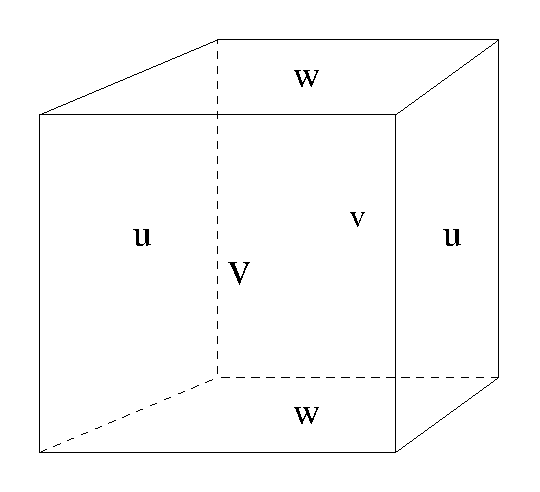
\includegraphics{part2/cgrid3d.eps}}
\end{center}
\caption{Three dimensional staggering of velocity components. This
facilitates the natural discretization of the continuity and tracer
equations. }
\label{fig:cgrid3d}
\end{figure}

The basic algorithm employed for stepping forward the momentum
equations is based on retaining non-divergence of the flow at all
times. This is most naturally done if the components of flow are
staggered in space in the form of an Arakawa C grid \cite{arakawa:77}.

Fig. \ref{fig:cgrid3d} shows the components of flow ($u$,$v$,$w$)
staggered in space such that the zonal component falls on the
interface between continuity cells in the zonal direction. Similarly
for the meridional and vertical directions.  The continuity cell is
synonymous with tracer cells (they are one and the same).



\subsection{Grid initialization and data}

Initialization of grid data is controlled by subroutine {\em
INI\_GRID} which in calls {\em INI\_VERTICAL\_GRID} to initialize the
vertical grid, and then either of {\em INI\_CARTESIAN\_GRID}, {\em
INI\_SPHERICAL\_POLAR\_GRID} or {\em INI\_CURV\-ILINEAR\_GRID} to
initialize the horizontal grid for cartesian, spherical-polar or
curvilinear coordinates respectively.

The reciprocals of all grid quantities are pre-calculated and this is
done in subroutine {\em INI\_MASKS\_ETC} which is called later by
subroutine {\em INITIALIZE\_FIXED}.

All grid descriptors are global arrays and stored in common blocks in
{\em GRID.h} and a generally declared as {\em \_RS}.

\fbox{ \begin{minipage}{4.75in}
{\em S/R INI\_GRID} ({\em model/src/ini\_grid.F})

{\em S/R INI\_MASKS\_ETC} ({\em model/src/ini\_masks\_etc.F})

grid data: ({\em model/inc/GRID.h})
\end{minipage} }


\subsection{Horizontal grid}
\label{sec:spatial_discrete_horizontal_grid}

\begin{figure}
\begin{center}
\begin{tabular}{cc}
  \raisebox{1.5in}{a)}\resizebox{!}{2in}{ 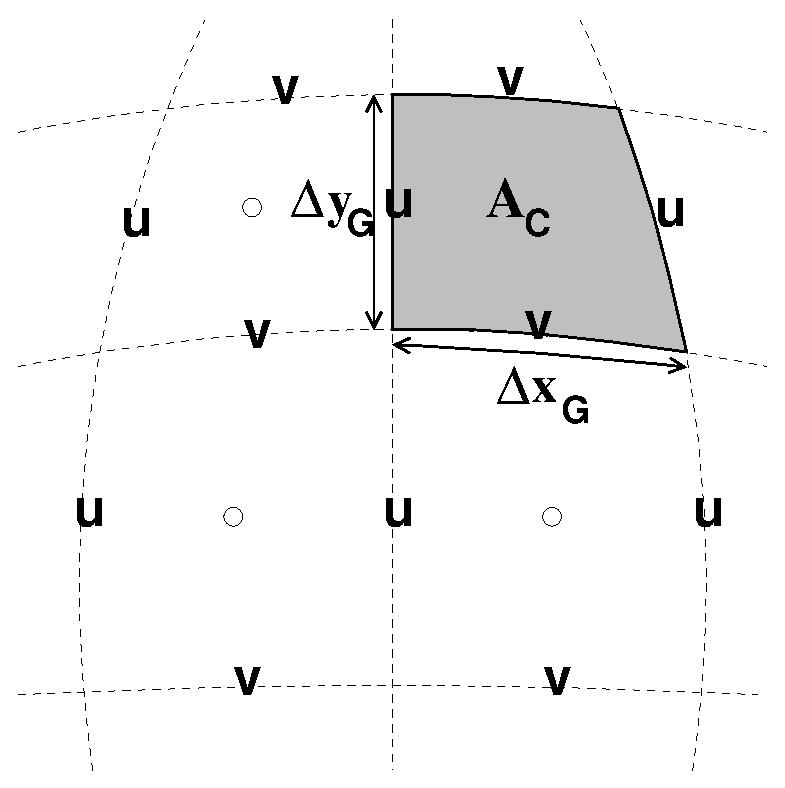
\includegraphics{part2/hgrid-Ac.eps}}
& \raisebox{1.5in}{b)}\resizebox{!}{2in}{ 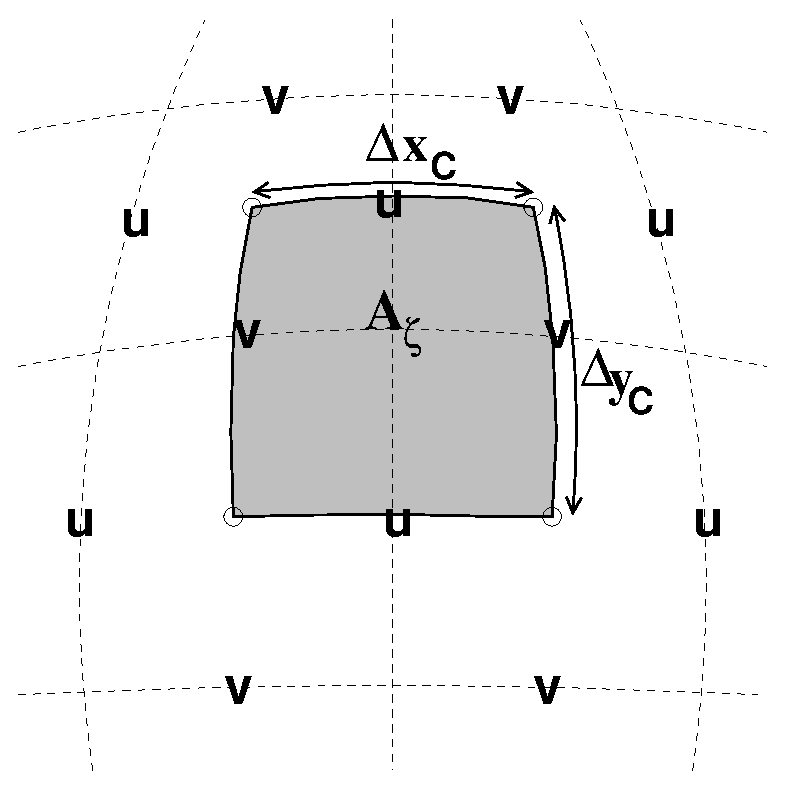
\includegraphics{part2/hgrid-Az.eps}}
\\
  \raisebox{1.5in}{c)}\resizebox{!}{2in}{ 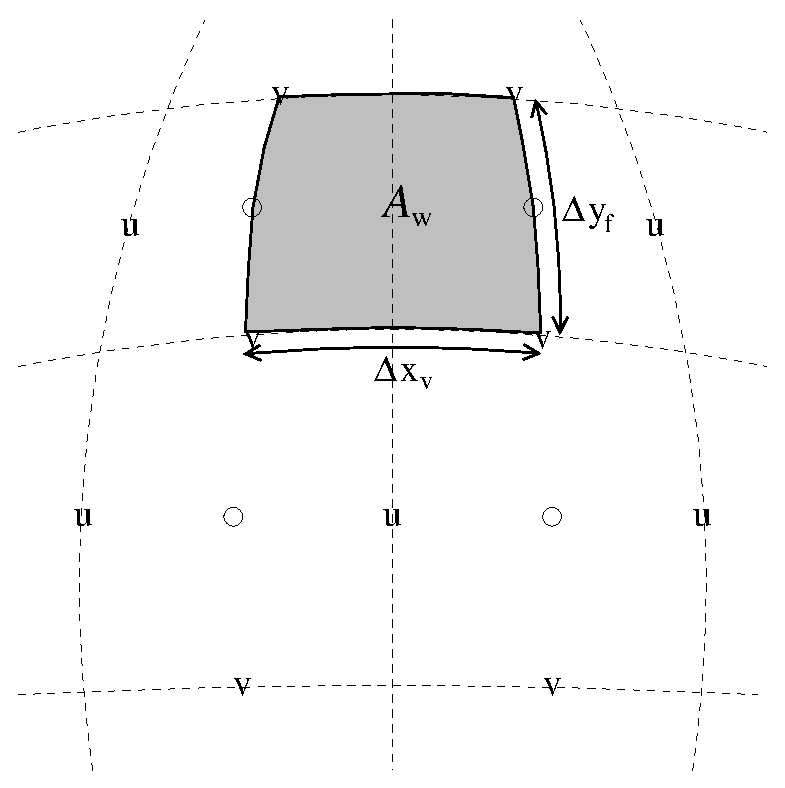
\includegraphics{part2/hgrid-Au.eps}}
& \raisebox{1.5in}{d)}\resizebox{!}{2in}{ 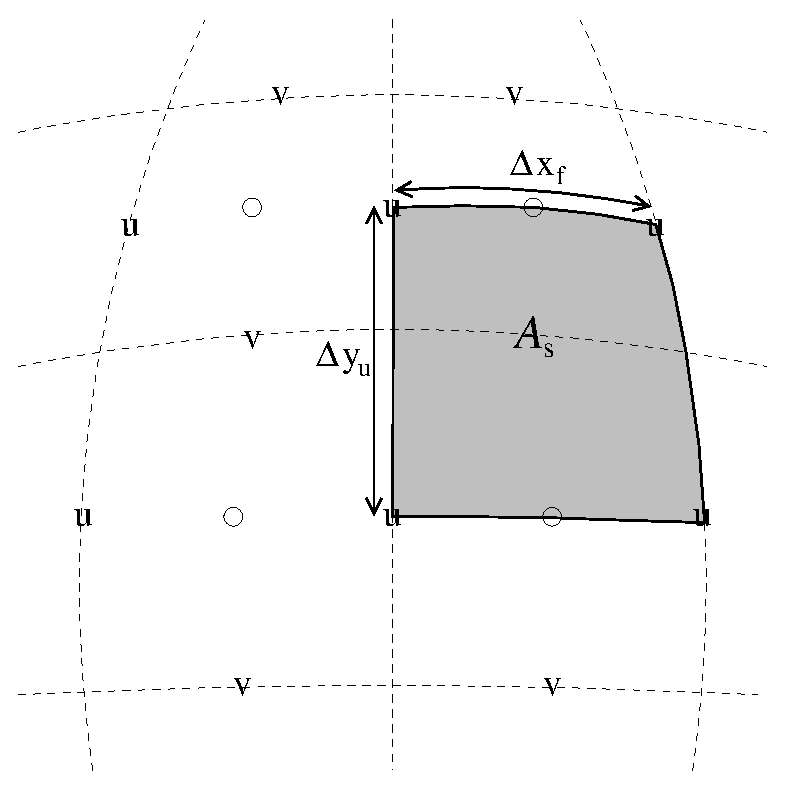
\includegraphics{part2/hgrid-Av.eps}}
\end{tabular}
\end{center}
\caption{
Staggering of horizontal grid descriptors (lengths and areas). The
grid lines indicate the tracer cell boundaries and are the reference
grid for all panels. a) The area of a tracer cell, $A_c$, is bordered
by the lengths $\Delta x_g$ and $\Delta y_g$. b) The area of a
vorticity cell, $A_\zeta$, is bordered by the lengths $\Delta x_c$ and
$\Delta y_c$. c) The area of a u cell, $A_c$, is bordered by the
lengths $\Delta x_v$ and $\Delta y_f$. d) The area of a v cell, $A_c$,
is bordered by the lengths $\Delta x_f$ and $\Delta y_u$.}
\label{fig:hgrid}
\end{figure}

The model domain is decomposed into tiles and within each tile a
quasi-regular grid is used. A tile is the basic unit of domain
decomposition for parallelization but may be used whether parallelized
or not; see section \ref{sect:tiles} for more details. Although the
tiles may be patched together in an unstructured manner
(i.e. irregular or non-tessilating pattern), the interior of tiles is
a structured grid of quadrilateral cells. The horizontal coordinate
system is orthogonal curvilinear meaning we can not necessarily treat
the two horizontal directions as separable. Instead, each cell in the
horizontal grid is described by the length of it's sides and it's
area.

The grid information is quite general and describes any of the
available coordinates systems, cartesian, spherical-polar or
curvilinear. All that is necessary to distinguish between the
coordinate systems is to initialize the grid data (descriptors)
appropriately.

In the following, we refer to the orientation of quantities on the
computational grid using geographic terminology such as points of the
compass.
\marginpar{Caution!}
This is purely for convenience but should note be confused
with the actual geographic orientation of model quantities.

Fig.~\ref{fig:hgrid}a shows the tracer cell (synonymous with the
continuity cell). The length of the southern edge, $\Delta x_g$,
western edge, $\Delta y_g$ and surface area, $A_c$, presented in the
vertical are stored in arrays {\bf DXg}, {\bf DYg} and {\bf rAc}.
\marginpar{$A_c$: {\bf rAc}}
\marginpar{$\Delta x_g$: {\bf DXg}}
\marginpar{$\Delta y_g$: {\bf DYg}}
The ``g'' suffix indicates that the lengths are along the defining
grid boundaries. The ``c'' suffix associates the quantity with the
cell centers. The quantities are staggered in space and the indexing
is such that {\bf DXg(i,j)} is positioned to the south of {\bf
rAc(i,j)} and {\bf DYg(i,j)} positioned to the west.

Fig.~\ref{fig:hgrid}b shows the vorticity cell. The length of the
southern edge, $\Delta x_c$, western edge, $\Delta y_c$ and surface
area, $A_\zeta$, presented in the vertical are stored in arrays {\bf
DXg}, {\bf DYg} and {\bf rAz}.
\marginpar{$A_\zeta$: {\bf rAz}}
\marginpar{$\Delta x_c$: {\bf DXc}}
\marginpar{$\Delta y_c$: {\bf DYc}}
The ``z'' suffix indicates that the lengths are measured between the
cell centers and the ``$\zeta$'' suffix associates points with the
vorticity points. The quantities are staggered in space and the
indexing is such that {\bf DXc(i,j)} is positioned to the north of
{\bf rAc(i,j)} and {\bf DYc(i,j)} positioned to the east.

Fig.~\ref{fig:hgrid}c shows the ``u'' or western (w) cell. The length of
the southern edge, $\Delta x_v$, eastern edge, $\Delta y_f$ and
surface area, $A_w$, presented in the vertical are stored in arrays
{\bf DXv}, {\bf DYf} and {\bf rAw}. 
\marginpar{$A_w$: {\bf rAw}}
\marginpar{$\Delta x_v$: {\bf DXv}}
\marginpar{$\Delta y_f$: {\bf DYf}}
The ``v'' suffix indicates that the length is measured between the
v-points, the ``f'' suffix indicates that the length is measured
between the (tracer) cell faces and the ``w'' suffix associates points
with the u-points (w stands for west). The quantities are staggered in
space and the indexing is such that {\bf DXv(i,j)} is positioned to
the south of {\bf rAw(i,j)} and {\bf DYf(i,j)} positioned to the east.

Fig.~\ref{fig:hgrid}d shows the ``v'' or southern (s) cell. The length of
the northern edge, $\Delta x_f$, western edge, $\Delta y_u$ and
surface area, $A_s$, presented in the vertical are stored in arrays
{\bf DXf}, {\bf DYu} and {\bf rAs}. 
\marginpar{$A_s$: {\bf rAs}}
\marginpar{$\Delta x_f$: {\bf DXf}}
\marginpar{$\Delta y_u$: {\bf DYu}}
The ``u'' suffix indicates that the length is measured between the
u-points, the ``f'' suffix indicates that the length is measured
between the (tracer) cell faces and the ``s'' suffix associates points
with the v-points (s stands for south). The quantities are staggered
in space and the indexing is such that {\bf DXf(i,j)} is positioned to
the north of {\bf rAs(i,j)} and {\bf DYu(i,j)} positioned to the west.

\fbox{ \begin{minipage}{4.75in}
{\em S/R INI\_CARTESIAN\_GRID} ({\em
model/src/ini\_cartesian\_grid.F})

{\em S/R INI\_SPHERICAL\_POLAR\_GRID} ({\em
model/src/ini\_spherical\_polar\_grid.F})

{\em S/R INI\_CURVILINEAR\_GRID} ({\em
model/src/ini\_curvilinear\_grid.F})

$A_c$, $A_\zeta$, $A_w$, $A_s$: {\bf rAc}, {\bf rAz}, {\bf rAw}, {\bf rAs}
({\em GRID.h})

$\Delta x_g$, $\Delta y_g$: {\bf DXg}, {\bf DYg} ({\em GRID.h})

$\Delta x_c$, $\Delta y_c$: {\bf DXc}, {\bf DYc} ({\em GRID.h})

$\Delta x_f$, $\Delta y_f$: {\bf DXf}, {\bf DYf} ({\em GRID.h})

$\Delta x_v$, $\Delta y_u$: {\bf DXv}, {\bf DYu} ({\em GRID.h})

\end{minipage} }

\subsubsection{Reciprocals of horizontal grid descriptors}

%\marginpar{$A_c^{-1}$: {\bf RECIP\_rAc}}
%\marginpar{$A_\zeta^{-1}$: {\bf RECIP\_rAz}}
%\marginpar{$A_w^{-1}$: {\bf RECIP\_rAw}}
%\marginpar{$A_s^{-1}$: {\bf RECIP\_rAs}}
Lengths and areas appear in the denominator of expressions as much as
in the numerator. For efficiency and portability, we pre-calculate the
reciprocal of the horizontal grid quantities so that in-line divisions
can be avoided.

%\marginpar{$\Delta x_g^{-1}$: {\bf RECIP\_DXg}}
%\marginpar{$\Delta y_g^{-1}$: {\bf RECIP\_DYg}}
%\marginpar{$\Delta x_c^{-1}$: {\bf RECIP\_DXc}}
%\marginpar{$\Delta y_c^{-1}$: {\bf RECIP\_DYc}}
%\marginpar{$\Delta x_f^{-1}$: {\bf RECIP\_DXf}}
%\marginpar{$\Delta y_f^{-1}$: {\bf RECIP\_DYf}}
%\marginpar{$\Delta x_v^{-1}$: {\bf RECIP\_DXv}}
%\marginpar{$\Delta y_u^{-1}$: {\bf RECIP\_DYu}}
For each grid descriptor (array) there is a reciprocal named using the
prefix {\bf RECIP\_}. This doubles the amount of storage in {\em
GRID.h} but they are all only 2-D descriptors.

\fbox{ \begin{minipage}{4.75in}
{\em S/R INI\_MASKS\_ETC} ({\em
model/src/ini\_masks\_etc.F})

$A_c^{-1}$: {\bf RECIP\_Ac} ({\em GRID.h})

$A_\zeta^{-1}$: {\bf RECIP\_Az} ({\em GRID.h})

$A_w^{-1}$: {\bf RECIP\_Aw} ({\em GRID.h})

$A_s^{-1}$: {\bf RECIP\_As} ({\em GRID.h})

$\Delta x_g^{-1}$, $\Delta y_g^{-1}$: {\bf RECIP\_DXg}, {\bf RECIP\_DYg} ({\em GRID.h})

$\Delta x_c^{-1}$, $\Delta y_c^{-1}$: {\bf RECIP\_DXc}, {\bf RECIP\_DYc} ({\em GRID.h})

$\Delta x_f^{-1}$, $\Delta y_f^{-1}$: {\bf RECIP\_DXf}, {\bf RECIP\_DYf} ({\em GRID.h})

$\Delta x_v^{-1}$, $\Delta y_u^{-1}$: {\bf RECIP\_DXv}, {\bf RECIP\_DYu} ({\em GRID.h})

\end{minipage} }

\subsubsection{Cartesian coordinates}

Cartesian coordinates are selected when the logical flag {\bf
using\-Cartes\-ianGrid} in namelist {\em PARM04} is set to true. The grid
spacing can be set to uniform via scalars {\bf dXspacing} and {\bf
dYspacing} in namelist {\em PARM04} or to variable resolution by the
vectors {\bf DELX} and {\bf DELY}. Units are normally
meters. Non-dimensional coordinates can be used by interpreting the
gravitational constant as the Rayleigh number.

\subsubsection{Spherical-polar coordinates}

Spherical coordinates are selected when the logical flag {\bf
using\-Spherical\-PolarGrid} in namelist {\em PARM04} is set to true. The
grid spacing can be set to uniform via scalars {\bf dXspacing} and
{\bf dYspacing} in namelist {\em PARM04} or to variable resolution by
the vectors {\bf DELX} and {\bf DELY}. Units of these namelist
variables are alway degrees. The horizontal grid descriptors are
calculated from these namelist variables have units of meters.

\subsubsection{Curvilinear coordinates}

Curvilinear coordinates are selected when the logical flag {\bf
using\-Curvil\-inear\-Grid} in namelist {\em PARM04} is set to true. The
grid spacing can not be set via the namelist. Instead, the grid
descriptors are read from data files, one for each descriptor. As for
other grids, the horizontal grid descriptors have units of meters.


\subsection{Vertical grid}

\begin{figure}
\begin{center}
  \begin{tabular}{cc}
  \raisebox{4in}{a)} \resizebox{!}{4in}{
  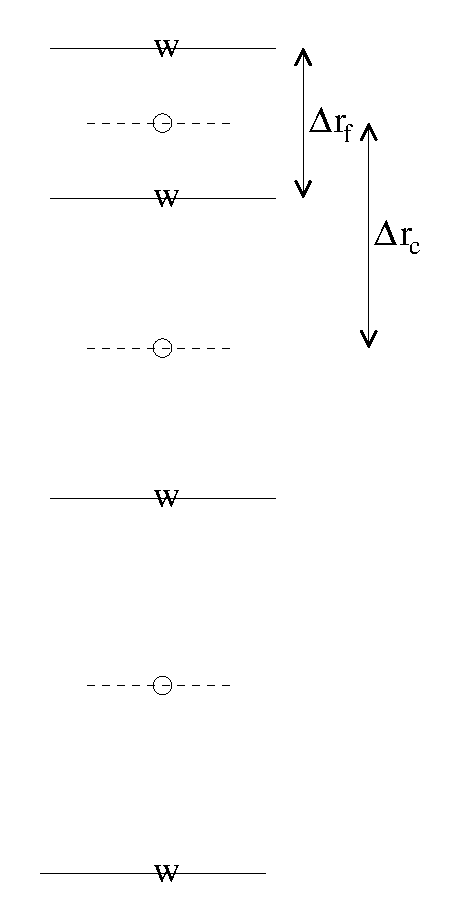
\includegraphics{part2/vgrid-cellcentered.eps}} & \raisebox{4in}{b)}
  \resizebox{!}{4in}{ 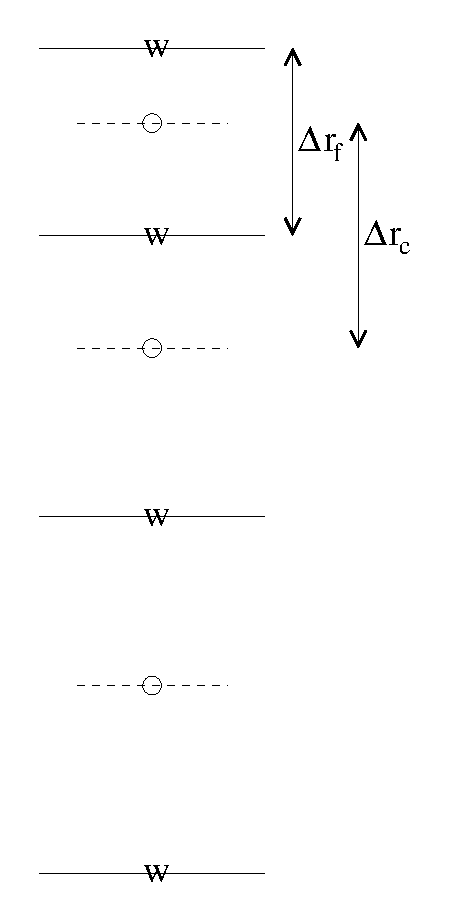
\includegraphics{part2/vgrid-accurate.eps}}
\end{tabular} 
\end{center}
\caption{Two versions of the vertical grid. a) The cell centered
approach where the interface depths are specified and the tracer
points centered in between the interfaces. b) The interface centered
approach where tracer levels are specified and the w-interfaces are
centered in between.}
\label{fig:vgrid}
\end{figure}

As for the horizontal grid, we use the suffixes ``c'' and ``f'' to
indicates faces and centers. Fig.~\ref{fig:vgrid}a shows the default
vertical grid used by the model.
\marginpar{$\Delta r_f$: {\bf DRf}}
\marginpar{$\Delta r_c$: {\bf DRc}}
$\Delta r_f$ is the difference in $r$
(vertical coordinate) between the faces (i.e. $\Delta r_f \equiv -
\delta_k r$ where the minus sign appears due to the convention that the
surface layer has index $k=1$.).

The vertical grid is calculated in subroutine {\em
INI\_VERTICAL\_GRID} and specified via the vector {\bf DELR} in
namelist {\em PARM04}. The units of ``r'' are either meters or Pascals
depending on the isomorphism being used which in turn is dependent
only on the choice of equation of state.

There are alternative namelist vectors {\bf DELZ} and {\bf DELP} which
dictate whether z- or
\marginpar{Caution!}
p- coordinates are to be used but we intend to
phase this out since they are redundant.

The reciprocals $\Delta r_f^{-1}$ and $\Delta r_c^{-1}$ are
pre-calculated (also in subroutine {\em INI\_VERTICAL\_GRID}). All
vertical grid descriptors are stored in common blocks in {\em GRID.h}.

The above grid (Fig.~\ref{fig:vgrid}a) is known as the cell centered
approach because the tracer points are at cell centers; the cell
centers are mid-way between the cell interfaces. 
This discretisation is selected when the thickness of the
levels are provided ({\bf delR}, parameter file {\em data}, 
namelist {\em PARM04})
An alternative, the vertex or interface centered approach, is shown in
Fig.~\ref{fig:vgrid}b. Here, the interior interfaces are positioned
mid-way between the tracer nodes (no longer cell centers). This
approach is formally more accurate for evaluation of hydrostatic
pressure and vertical advection but historically the cell centered
approach has been used. An alternative form of subroutine {\em
INI\_VERTICAL\_GRID} is used to select the interface centered approach
This form requires to specify $Nr+1$ vertical distances {\bf delRc} 
(parameter file {\em data}, namelist {\em PARM04}, e.g. 
{\em verification/ideal\_2D\_oce/input/data})
corresponding to surface to center, $Nr-1$ center to center, and center to 
bottom distances.
%but no run time option is currently available.

\fbox{ \begin{minipage}{4.75in}
{\em S/R INI\_VERTICAL\_GRID} ({\em
model/src/ini\_vertical\_grid.F})

$\Delta r_f$: {\bf DRf} ({\em GRID.h})

$\Delta r_c$: {\bf DRc} ({\em GRID.h})

$\Delta r_f^{-1}$: {\bf RECIP\_DRf} ({\em GRID.h})

$\Delta r_c^{-1}$: {\bf RECIP\_DRc} ({\em GRID.h})

\end{minipage} }


\subsection{Topography: partially filled cells}
\begin{rawhtml}
<!-- CMIREDIR:topo_partial_cells: -->
\end{rawhtml}

\begin{figure}
\begin{center}
\resizebox{4.5in}{!}{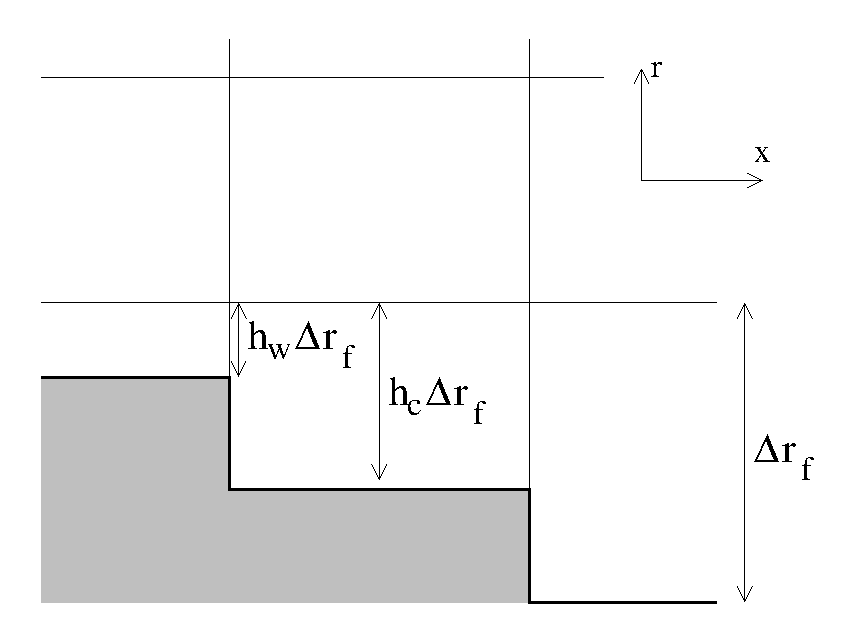
\includegraphics{part2/vgrid-xz.eps}}
\end{center}
\caption{
A schematic of the x-r plane showing the location of the
non-dimensional fractions $h_c$ and $h_w$. The physical thickness of a
tracer cell is given by $h_c(i,j,k) \Delta r_f(k)$ and the physical
thickness of the open side is given by $h_w(i,j,k) \Delta r_f(k)$.}
\label{fig:hfacs}
\end{figure}

\cite{adcroft:97} presented two alternatives to the step-wise finite
difference representation of topography. The method is known to the
engineering community as {\em intersecting boundary method}. It
involves allowing the boundary to intersect a grid of cells thereby
modifying the shape of those cells intersected. We suggested allowing
the topography to take on a piece-wise linear representation (shaved
cells) or a simpler piecewise constant representation (partial step).
Both show dramatic improvements in solution compared to the
traditional full step representation, the piece-wise linear being the
best. However, the storage requirements are excessive so the simpler
piece-wise constant or partial-step method is all that is currently
supported.

Fig.~\ref{fig:hfacs} shows a schematic of the x-r plane indicating how
the thickness of a level is determined at tracer and u points.
\marginpar{$h_c$: {\bf hFacC}}
\marginpar{$h_w$: {\bf hFacW}}
\marginpar{$h_s$: {\bf hFacS}}
The physical thickness of a tracer cell is given by $h_c(i,j,k) \Delta
r_f(k)$ and the physical thickness of the open side is given by
$h_w(i,j,k) \Delta r_f(k)$. Three 3-D descriptors $h_c$, $h_w$ and
$h_s$ are used to describe the geometry: {\bf hFacC}, {\bf hFacW} and
{\bf hFacS} respectively. These are calculated in subroutine {\em
INI\_MASKS\_ETC} along with there reciprocals {\bf RECIP\_hFacC}, {\bf
RECIP\_hFacW} and {\bf RECIP\_hFacS}.

The non-dimensional fractions (or h-facs as we call them) are
calculated from the model depth array and then processed to avoid tiny
volumes. The rule is that if a fraction is less than {\bf hFacMin}
then it is rounded to the nearer of $0$ or {\bf hFacMin} or if the
physical thickness is less than {\bf hFacMinDr} then it is similarly
rounded. The larger of the two methods is used when there is a
conflict. By setting {\bf hFacMinDr} equal to or larger than the
thinnest nominal layers, $\min{(\Delta z_f)}$, but setting {\bf
hFacMin} to some small fraction then the model will only lop thick
layers but retain stability based on the thinnest unlopped thickness;
$\min{(\Delta z_f,\mbox{\bf hFacMinDr})}$.

\fbox{ \begin{minipage}{4.75in}
{\em S/R INI\_MASKS\_ETC} ({\em model/src/ini\_masks\_etc.F})

$h_c$: {\bf hFacC} ({\em GRID.h})

$h_w$: {\bf hFacW} ({\em GRID.h})

$h_s$: {\bf hFacS} ({\em GRID.h})

$h_c^{-1}$: {\bf RECIP\_hFacC} ({\em GRID.h})

$h_w^{-1}$: {\bf RECIP\_hFacW} ({\em GRID.h})

$h_s^{-1}$: {\bf RECIP\_hFacS} ({\em GRID.h})

\end{minipage} }


\section{Continuity and horizontal pressure gradient terms}

The core algorithm is based on the ``C grid'' discretization of the
continuity equation which can be summarized as:
\begin{eqnarray}
\partial_t u + \frac{1}{\Delta x_c} \delta_i \left. \frac{ \partial \Phi}{\partial r}\right|_{s} \eta + \frac{\epsilon_{nh}}{\Delta x_c} \delta_i \Phi_{nh}' & = & G_u - \frac{1}{\Delta x_c} \delta_i \Phi_h' \label{eq:discrete-momu} \\
\partial_t v + \frac{1}{\Delta y_c} \delta_j \left. \frac{ \partial \Phi}{\partial r}\right|_{s} \eta + \frac{\epsilon_{nh}}{\Delta y_c} \delta_j \Phi_{nh}' & = & G_v - \frac{1}{\Delta y_c} \delta_j \Phi_h' \label{eq:discrete-momv} \\
\epsilon_{nh} \left( \partial_t w + \frac{1}{\Delta r_c} \delta_k \Phi_{nh}' \right) & = & \epsilon_{nh} G_w + \overline{b}^k - \frac{1}{\Delta r_c} \delta_k \Phi_{h}' \label{eq:discrete-momw} \\
\delta_i \Delta y_g \Delta r_f h_w u +
\delta_j \Delta x_g \Delta r_f h_s v +
\delta_k {\cal A}_c w & = & {\cal A}_c \delta_k (P-E)_{r=0}
\label{eq:discrete-continuity}
\end{eqnarray}
where the continuity equation has been most naturally discretized by
staggering the three components of velocity as shown in
Fig.~\ref{fig:cgrid3d}. The grid lengths $\Delta x_c$ and $\Delta y_c$
are the lengths between tracer points (cell centers). The grid lengths
$\Delta x_g$, $\Delta y_g$ are the grid lengths between cell
corners. $\Delta r_f$ and $\Delta r_c$ are the distance (in units of
$r$) between level interfaces (w-level) and level centers (tracer
level). The surface area presented in the vertical is denoted ${\cal
A}_c$.  The factors $h_w$ and $h_s$ are non-dimensional fractions
(between 0 and 1) that represent the fraction cell depth that is
``open'' for fluid flow.
\marginpar{$h_w$: {\bf hFacW}}
\marginpar{$h_s$: {\bf hFacS}}

The last equation, the discrete continuity equation, can be summed in
the vertical to yield the free-surface equation:
\begin{equation}
{\cal A}_c \partial_t \eta + \delta_i \sum_k \Delta y_g \Delta r_f h_w
u + \delta_j \sum_k \Delta x_g \Delta r_f h_s v = {\cal
A}_c(P-E)_{r=0} \label{eq:discrete-freesurface}
\end{equation}
The source term $P-E$ on the rhs of continuity accounts for the local
addition of volume due to excess precipitation and run-off over
evaporation and only enters the top-level of the {\em ocean} model.

\section{Hydrostatic balance}

The vertical momentum equation has the hydrostatic or
quasi-hydrostatic balance on the right hand side. This discretization
guarantees that the conversion of potential to kinetic energy as
derived from the buoyancy equation exactly matches the form derived
from the pressure gradient terms when forming the kinetic energy
equation.

In the ocean, using z-coordinates, the hydrostatic balance terms are
discretized:
\begin{equation}
\epsilon_{nh} \partial_t w
+ g \overline{\rho'}^k + \frac{1}{\Delta z} \delta_k \Phi_h' = \ldots
\label{eq:discrete_hydro_ocean}
\end{equation}

In the atmosphere, using p-coordinates, hydrostatic balance is
discretized:
\begin{equation}
\overline{\theta'}^k + \frac{1}{\Delta \Pi} \delta_k \Phi_h' = 0
\label{eq:discrete_hydro_atmos}
\end{equation}
where $\Delta \Pi$ is the difference in Exner function between the
pressure points. The non-hydrostatic equations are not available in
the atmosphere.

The difference in approach between ocean and atmosphere occurs because
of the direct use of the ideal gas equation in forming the potential
energy conversion term $\alpha \omega$. The form of these conversion
terms is discussed at length in \cite{adcroft:02}.

Because of the different representation of hydrostatic balance between
ocean and atmosphere there is no elegant way to represent both systems
using an arbitrary coordinate.

The integration for hydrostatic pressure is made in the positive $r$
direction (increasing k-index). For the ocean, this is from the
free-surface down and for the atmosphere this is from the ground up.

The calculations are made in the subroutine {\em
CALC\_PHI\_HYD}. Inside this routine, one of other of the
atmospheric/oceanic form is selected based on the string variable {\bf
buoyancyRelation}.


% $Header: /u/gcmpack/manual/s_algorithm/text/mom_fluxform.tex,v 1.14 2010/08/30 23:09:18 jmc Exp $
% $Name:  $

\section{Flux-form momentum equations}
\label{sec:flux-form_momentum_equations}
\begin{rawhtml}
<!-- CMIREDIR:flux-form_momentum_equations: -->
\end{rawhtml}

The original finite volume model was based on the Eulerian flux form
momentum equations. This is the default though the vector invariant
form is optionally available (and recommended in some cases).

The ``G's'' (our colloquial name for all terms on rhs!) are broken
into the various advective, Coriolis, horizontal dissipation, vertical
dissipation and metric forces:
\marginpar{$G_u$: {\bf Gu} }
\marginpar{$G_v$: {\bf Gv} }
\marginpar{$G_w$: {\bf Gw} }
\begin{eqnarray}
G_u & = & G_u^{adv} + G_u^{cor} + G_u^{h-diss} + G_u^{v-diss} +
G_u^{metric} + G_u^{nh-metric} \label{eq:gsplit_momu} \\
G_v & = & G_v^{adv} + G_v^{cor} + G_v^{h-diss} + G_v^{v-diss} +
G_v^{metric} + G_v^{nh-metric} \label{eq:gsplit_momv} \\
G_w & = & G_w^{adv} + G_w^{cor} + G_w^{h-diss} + G_w^{v-diss} +
G_w^{metric} + G_w^{nh-metric} \label{eq:gsplit_momw}
\end{eqnarray}
In the hydrostatic limit, $G_w=0$ and $\epsilon_{nh}=0$, reducing the
vertical momentum to hydrostatic balance.

These terms are calculated in routines called from subroutine {\em
MOM\_FLUXFORM} a collected into the global arrays {\bf Gu}, {\bf Gv},
and {\bf Gw}.

\fbox{ \begin{minipage}{4.75in}
{\em S/R MOM\_FLUXFORM} ({\em pkg/mom\_fluxform/mom\_fluxform.F})

$G_u$: {\bf Gu} ({\em DYNVARS.h})

$G_v$: {\bf Gv} ({\em DYNVARS.h})

$G_w$: {\bf Gw} ({\em DYNVARS.h})
\end{minipage} }


\subsection{Advection of momentum}

The advective operator is second order accurate in space:
\begin{eqnarray}
{\cal A}_w \Delta r_f h_w G_u^{adv} & = &
  \delta_i \overline{ U }^i \overline{ u }^i
+ \delta_j \overline{ V }^i \overline{ u }^j
+ \delta_k \overline{ W }^i \overline{ u }^k \label{eq:discrete-momadvu} \\
{\cal A}_s \Delta r_f h_s G_v^{adv} & = &
  \delta_i \overline{ U }^j \overline{ v }^i
+ \delta_j \overline{ V }^j \overline{ v }^j
+ \delta_k \overline{ W }^j \overline{ v }^k \label{eq:discrete-momadvv} \\
{\cal A}_c \Delta r_c G_w^{adv} & = &
  \delta_i \overline{ U }^k \overline{ w }^i
+ \delta_j \overline{ V }^k \overline{ w }^j
+ \delta_k \overline{ W }^k \overline{ w }^k \label{eq:discrete-momadvw}
\end{eqnarray}
and because of the flux form does not contribute to the global budget
of linear momentum. The quantities $U$, $V$ and $W$ are volume fluxes
defined:
\marginpar{$U$: {\bf uTrans} }
\marginpar{$V$: {\bf vTrans} }
\marginpar{$W$: {\bf rTrans} }
\begin{eqnarray}
U & = & \Delta y_g \Delta r_f h_w u \label{eq:utrans} \\
V & = & \Delta x_g \Delta r_f h_s v \label{eq:vtrans} \\
W & = & {\cal A}_c w \label{eq:rtrans}
\end{eqnarray}
The advection of momentum takes the same form as the advection of
tracers but by a translated advective flow. Consequently, the
conservation of second moments, derived for tracers later, applies to
$u^2$ and $v^2$ and $w^2$ so that advection of momentum correctly
conserves kinetic energy.

\fbox{ \begin{minipage}{4.75in}
{\em S/R MOM\_U\_ADV\_UU} ({\em mom\_u\_adv\_uu.F})

{\em S/R MOM\_U\_ADV\_VU} ({\em mom\_u\_adv\_vu.F})

{\em S/R MOM\_U\_ADV\_WU} ({\em mom\_u\_adv\_wu.F})

{\em S/R MOM\_U\_ADV\_UV} ({\em mom\_u\_adv\_uv.F})

{\em S/R MOM\_U\_ADV\_VV} ({\em mom\_u\_adv\_vv.F})

{\em S/R MOM\_U\_ADV\_WV} ({\em mom\_u\_adv\_wv.F})

$uu$, $uv$, $vu$, $vv$: {\bf aF} (local to {\em mom\_fluxform.F})
\end{minipage} }



\subsection{Coriolis terms}

The ``pure C grid'' Coriolis terms (i.e. in absence of C-D scheme) are
discretized:
\begin{eqnarray}
{\cal A}_w \Delta r_f h_w G_u^{Cor} & = &
  \overline{ f {\cal A}_c \Delta r_f h_c \overline{ v }^j }^i
- \epsilon_{nh} \overline{ f' {\cal A}_c \Delta r_f h_c \overline{ w }^k }^i \\
{\cal A}_s \Delta r_f h_s G_v^{Cor} & = &
- \overline{ f {\cal A}_c \Delta r_f h_c \overline{ u }^i }^j \\
{\cal A}_c \Delta r_c G_w^{Cor} & = &
 \epsilon_{nh} \overline{ f' {\cal A}_c \Delta r_f h_c \overline{ u }^i }^k
\end{eqnarray}
where the Coriolis parameters $f$ and $f'$ are defined:
\begin{eqnarray}
f & = & 2 \Omega \sin{\varphi} \\
f' & = & 2 \Omega \cos{\varphi}
\end{eqnarray}
where $\varphi$ is geographic latitude when using spherical geometry,
otherwise the $\beta$-plane definition is used:
\begin{eqnarray}
f & = & f_o + \beta y \\
f' & = & 0
\end{eqnarray}

This discretization globally conserves kinetic energy. It should be
noted that despite the use of this discretization in former
publications, all calculations to date have used the following
different discretization:
\begin{eqnarray}
G_u^{Cor} & = &
  f_u \overline{ v }^{ji}
- \epsilon_{nh} f_u' \overline{ w }^{ik} \\
G_v^{Cor} & = &
- f_v \overline{ u }^{ij} \\
G_w^{Cor} & = &
 \epsilon_{nh} f_w' \overline{ u }^{ik}
\end{eqnarray}
\marginpar{Need to change the default in code to match this}
where the subscripts on $f$ and $f'$ indicate evaluation of the
Coriolis parameters at the appropriate points in space. The above
discretization does {\em not} conserve anything, especially energy and
for historical reasons is the default for the code. A
flag controls this discretization: set run-time logical {\bf
useEnergyConservingCoriolis} to {\em true} which otherwise defaults to
{\em false}.

\fbox{ \begin{minipage}{4.75in}
{\em S/R MOM\_CDSCHEME} ({\em mom\_cdscheme.F})

{\em S/R MOM\_U\_CORIOLIS} ({\em mom\_u\_coriolis.F})

{\em S/R MOM\_V\_CORIOLIS} ({\em mom\_v\_coriolis.F})

$G_u^{Cor}$, $G_v^{Cor}$: {\bf cF} (local to {\em mom\_fluxform.F})
\end{minipage} }


\subsection{Curvature metric terms}

The most commonly used coordinate system on the sphere is the
geographic system $(\lambda,\varphi)$. The curvilinear nature of these
coordinates on the sphere lead to some ``metric'' terms in the
component momentum equations. Under the thin-atmosphere and
hydrostatic approximations these terms are discretized:
\begin{eqnarray}
{\cal A}_w \Delta r_f h_w G_u^{metric} & = &
  \overline{ \frac{ \overline{u}^i }{a} \tan{\varphi} {\cal A}_c \Delta r_f h_c \overline{ v }^j }^i \\
{\cal A}_s \Delta r_f h_s G_v^{metric} & = &
- \overline{ \frac{ \overline{u}^i }{a} \tan{\varphi} {\cal A}_c \Delta r_f h_c \overline{ u }^i }^j \\
G_w^{metric} & = & 0
\end{eqnarray}
where $a$ is the radius of the planet (sphericity is assumed) or the
radial distance of the particle (i.e. a function of height).  It is
easy to see that this discretization satisfies all the properties of
the discrete Coriolis terms since the metric factor $\frac{u}{a}
\tan{\varphi}$ can be viewed as a modification of the vertical Coriolis
parameter: $f \rightarrow f+\frac{u}{a} \tan{\varphi}$.

However, as for the Coriolis terms, a non-energy conserving form has
exclusively been used to date:
\begin{eqnarray}
G_u^{metric} & = & \frac{u \overline{v}^{ij} }{a} \tan{\varphi} \\
G_v^{metric} & = & \frac{ \overline{u}^{ij} \overline{u}^{ij}}{a} \tan{\varphi}
\end{eqnarray}
where $\tan{\varphi}$ is evaluated at the $u$ and $v$ points
respectively.

\fbox{ \begin{minipage}{4.75in}
{\em S/R MOM\_U\_METRIC\_SPHERE} ({\em mom\_u\_metric\_sphere.F})

{\em S/R MOM\_V\_METRIC\_SPHERE} ({\em mom\_v\_metric\_sphere.F})

$G_u^{metric}$, $G_v^{metric}$: {\bf mT} (local to {\em mom\_fluxform.F})
\end{minipage} }



\subsection{Non-hydrostatic metric terms}

For the non-hydrostatic equations, dropping the thin-atmosphere
approximation re-introduces metric terms involving $w$ and are
required to conserve angular momentum:
\begin{eqnarray}
{\cal A}_w \Delta r_f h_w G_u^{metric} & = &
- \overline{ \frac{ \overline{u}^i \overline{w}^k }{a} {\cal A}_c \Delta r_f h_c }^i \\
{\cal A}_s \Delta r_f h_s G_v^{metric} & = &
- \overline{ \frac{ \overline{v}^j \overline{w}^k }{a} {\cal A}_c \Delta r_f h_c}^j \\
{\cal A}_c \Delta r_c G_w^{metric} & = &
  \overline{ \frac{ {\overline{u}^i}^2 + {\overline{v}^j}^2}{a} {\cal A}_c \Delta r_f h_c }^k
\end{eqnarray}

Because we are always consistent, even if consistently wrong, we have,
in the past, used a different discretization in the model which is:
\begin{eqnarray}
G_u^{metric} & = &
- \frac{u}{a} \overline{w}^{ik} \\
G_v^{metric} & = &
- \frac{v}{a} \overline{w}^{jk} \\
G_w^{metric} & = &
  \frac{1}{a} ( {\overline{u}^{ik}}^2 + {\overline{v}^{jk}}^2 )
\end{eqnarray}

\fbox{ \begin{minipage}{4.75in}
{\em S/R MOM\_U\_METRIC\_NH} ({\em mom\_u\_metric\_nh.F})

{\em S/R MOM\_V\_METRIC\_NH} ({\em mom\_v\_metric\_nh.F})

$G_u^{metric}$, $G_v^{metric}$: {\bf mT} (local to {\em mom\_fluxform.F})
\end{minipage} }


\subsection{Lateral dissipation}

Historically, we have represented the SGS Reynolds stresses as simply
down gradient momentum fluxes, ignoring constraints on the stress
tensor such as symmetry.
\begin{eqnarray}
{\cal A}_w \Delta r_f h_w G_u^{h-diss} & = &
  \delta_i  \Delta y_f \Delta r_f h_c \tau_{11}
+ \delta_j  \Delta x_v \Delta r_f h_\zeta \tau_{12} \\
{\cal A}_s \Delta r_f h_s G_v^{h-diss} & = &
  \delta_i  \Delta y_u \Delta r_f h_\zeta \tau_{21}
+ \delta_j  \Delta x_f \Delta r_f h_c \tau_{22}
\end{eqnarray}
\marginpar{Check signs of stress definitions}

The lateral viscous stresses are discretized:
\begin{eqnarray}
\tau_{11} & = & A_h c_{11\Delta}(\varphi) \frac{1}{\Delta x_f} \delta_i u
               -A_4 c_{11\Delta^2}(\varphi) \frac{1}{\Delta x_f} \delta_i \nabla^2 u \\
\tau_{12} & = & A_h c_{12\Delta}(\varphi) \frac{1}{\Delta y_u} \delta_j u
               -A_4 c_{12\Delta^2}(\varphi)\frac{1}{\Delta y_u} \delta_j \nabla^2 u \\
\tau_{21} & = & A_h c_{21\Delta}(\varphi) \frac{1}{\Delta x_v} \delta_i v
               -A_4 c_{21\Delta^2}(\varphi) \frac{1}{\Delta x_v} \delta_i \nabla^2 v \\
\tau_{22} & = & A_h c_{22\Delta}(\varphi) \frac{1}{\Delta y_f} \delta_j v
               -A_4 c_{22\Delta^2}(\varphi) \frac{1}{\Delta y_f} \delta_j \nabla^2 v
\end{eqnarray}
where the non-dimensional factors $c_{lm\Delta^n}(\varphi), \{l,m,n\} \in
\{1,2\}$ define the ``cosine'' scaling with latitude which can be
applied in various ad-hoc ways. For instance, $c_{11\Delta} =
c_{21\Delta} = (\cos{\varphi})^{3/2}$, $c_{12\Delta}=c_{22\Delta}=1$ would
represent the an-isotropic cosine scaling typically used on the
``lat-lon'' grid for Laplacian viscosity.
\marginpar{Need to tidy up method for controlling this in code}

It should be noted that despite the ad-hoc nature of the scaling, some
scaling must be done since on a lat-lon grid the converging meridians
make it very unlikely that a stable viscosity parameter exists across
the entire model domain.

The Laplacian viscosity coefficient, $A_h$ ({\bf viscAh}), has units
of $m^2 s^{-1}$. The bi-harmonic viscosity coefficient, $A_4$ ({\bf
viscA4}), has units of $m^4 s^{-1}$.

\fbox{ \begin{minipage}{4.75in}
{\em S/R MOM\_U\_XVISCFLUX} ({\em mom\_u\_xviscflux.F})

{\em S/R MOM\_U\_YVISCFLUX} ({\em mom\_u\_yviscflux.F})

{\em S/R MOM\_V\_XVISCFLUX} ({\em mom\_v\_xviscflux.F})

{\em S/R MOM\_V\_YVISCFLUX} ({\em mom\_v\_yviscflux.F})

$\tau_{11}$, $\tau_{12}$, $\tau_{21}$, $\tau_{22}$: {\bf vF}, {\bf
v4F} (local to {\em mom\_fluxform.F})
\end{minipage} }

Two types of lateral boundary condition exist for the lateral viscous
terms, no-slip and free-slip.

The free-slip condition is most convenient to code since it is
equivalent to zero-stress on boundaries. Simple masking of the stress
components sets them to zero. The fractional open stress is properly
handled using the lopped cells.

The no-slip condition defines the normal gradient of a tangential flow
such that the flow is zero on the boundary. Rather than modify the
stresses by using complicated functions of the masks and ``ghost''
points (see \cite{adcroft:98}) we add the boundary stresses as
an additional source term in cells next to solid boundaries. This has
the advantage of being able to cope with ``thin walls'' and also makes
the interior stress calculation (code) independent of the boundary
conditions. The ``body'' force takes the form:
\begin{eqnarray}
G_u^{side-drag} & = &
\frac{4}{\Delta z_f} \overline{ (1-h_\zeta) \frac{\Delta x_v}{\Delta y_u} }^j
\left( A_h c_{12\Delta}(\varphi) u - A_4 c_{12\Delta^2}(\varphi) \nabla^2 u \right)
\\
G_v^{side-drag} & = &
\frac{4}{\Delta z_f} \overline{ (1-h_\zeta) \frac{\Delta y_u}{\Delta x_v} }^i
\left( A_h c_{21\Delta}(\varphi) v - A_4 c_{21\Delta^2}(\varphi) \nabla^2 v \right)
\end{eqnarray}

In fact, the above discretization is not quite complete because it
assumes that the bathymetry at velocity points is deeper than at
neighboring vorticity points, e.g. $1-h_w < 1-h_\zeta$

\fbox{ \begin{minipage}{4.75in}
{\em S/R MOM\_U\_SIDEDRAG} ({\em mom\_u\_sidedrag.F})

{\em S/R MOM\_V\_SIDEDRAG} ({\em mom\_v\_sidedrag.F})

$G_u^{side-drag}$, $G_v^{side-drag}$: {\bf vF} (local to {\em mom\_fluxform.F})
\end{minipage} }


\subsection{Vertical dissipation}

Vertical viscosity terms are discretized with only partial adherence
to the variable grid lengths introduced by the finite volume
formulation. This reduces the formal accuracy of these terms to just
first order but only next to boundaries; exactly where other terms
appear such as linear and quadratic bottom drag.
\begin{eqnarray}
G_u^{v-diss} & = &
\frac{1}{\Delta r_f h_w} \delta_k \tau_{13} \\
G_v^{v-diss} & = &
\frac{1}{\Delta r_f h_s} \delta_k \tau_{23} \\
G_w^{v-diss} & = & \epsilon_{nh}
\frac{1}{\Delta r_f h_d} \delta_k \tau_{33}
\end{eqnarray}
represents the general discrete form of the vertical dissipation terms.

In the interior the vertical stresses are discretized:
\begin{eqnarray}
\tau_{13} & = & A_v \frac{1}{\Delta r_c} \delta_k u \\
\tau_{23} & = & A_v \frac{1}{\Delta r_c} \delta_k v \\
\tau_{33} & = & A_v \frac{1}{\Delta r_f} \delta_k w
\end{eqnarray}
It should be noted that in the non-hydrostatic form, the stress tensor
is even less consistent than for the hydrostatic (see
\cite{wajsowicz:93}). It is well known how to do this properly (see 
\cite{griffies:00}) and is on the list of to-do's.

\fbox{ \begin{minipage}{4.75in}
{\em S/R MOM\_U\_RVISCLFUX} ({\em mom\_u\_rviscflux.F})

{\em S/R MOM\_V\_RVISCLFUX} ({\em mom\_v\_rviscflux.F})

$\tau_{13}$: {\bf urf} (local to {\em mom\_fluxform.F})

$\tau_{23}$: {\bf vrf} (local to {\em mom\_fluxform.F})
\end{minipage} }


As for the lateral viscous terms, the free-slip condition is
equivalent to simply setting the stress to zero on boundaries.  The
no-slip condition is implemented as an additional term acting on top
of the interior and free-slip stresses. Bottom drag represents
additional friction, in addition to that imposed by the no-slip
condition at the bottom. The drag is cast as a stress expressed as a
linear or quadratic function of the mean flow in the layer above the
topography:
\begin{eqnarray}
\tau_{13}^{bottom-drag} & = &
\left(
2 A_v \frac{1}{\Delta r_c}
+ r_b
+ C_d \sqrt{ \overline{2 KE}^i }
\right) u \\
\tau_{23}^{bottom-drag} & = &
\left(
2 A_v \frac{1}{\Delta r_c}
+ r_b
+ C_d \sqrt{ \overline{2 KE}^j }
\right) v
\end{eqnarray}
where these terms are only evaluated immediately above topography.
$r_b$ ({\bf bottomDragLinear}) has units of $m s^{-1}$ and a typical value
of the order 0.0002 $m s^{-1}$. $C_d$ ({\bf bottomDragQuadratic}) is
dimensionless with typical values in the range 0.001--0.003.

\fbox{ \begin{minipage}{4.75in}
{\em S/R MOM\_U\_BOTTOMDRAG} ({\em mom\_u\_bottomdrag.F})

{\em S/R MOM\_V\_BOTTOMDRAG} ({\em mom\_v\_bottomdrag.F})

$\tau_{13}^{bottom-drag}/\Delta r_f$, $\tau_{23}^{bottom-drag}/\Delta r_f$: 
{\bf vf} (local to {\em mom\_fluxform.F})
\end{minipage} }

\subsection{Derivation of discrete energy conservation}

These discrete equations conserve kinetic plus potential energy using the
following definitions:
\begin{equation}
KE = \frac{1}{2} \left( \overline{ u^2 }^i + \overline{ v^2 }^j +
\epsilon_{nh} \overline{ w^2 }^k \right)
\end{equation}

\subsection{Mom Diagnostics}
\label{sec:pkg:mom_common:diagnostics}

\begin{verbatim}

------------------------------------------------------------------------
<-Name->|Levs|<-parsing code->|<--  Units   -->|<- Tile (max=80c) 
------------------------------------------------------------------------
VISCAHZ | 15 |SZ      MR      |m^2/s           |Harmonic Visc Coefficient (m2/s) (Zeta Pt)
VISCA4Z | 15 |SZ      MR      |m^4/s           |Biharmonic Visc Coefficient (m4/s) (Zeta Pt)
VISCAHD | 15 |SM      MR      |m^2/s           |Harmonic Viscosity Coefficient (m2/s) (Div Pt)
VISCA4D | 15 |SM      MR      |m^4/s           |Biharmonic Viscosity Coefficient (m4/s) (Div Pt)
VAHZMAX | 15 |SZ      MR      |m^2/s           |CFL-MAX Harm Visc Coefficient (m2/s) (Zeta Pt)
VA4ZMAX | 15 |SZ      MR      |m^4/s           |CFL-MAX Biharm Visc Coefficient (m4/s) (Zeta Pt)
VAHDMAX | 15 |SM      MR      |m^2/s           |CFL-MAX Harm Visc Coefficient (m2/s) (Div Pt)
VA4DMAX | 15 |SM      MR      |m^4/s           |CFL-MAX Biharm Visc Coefficient (m4/s) (Div Pt)
VAHZMIN | 15 |SZ      MR      |m^2/s           |RE-MIN Harm Visc Coefficient (m2/s) (Zeta Pt)
VA4ZMIN | 15 |SZ      MR      |m^4/s           |RE-MIN Biharm Visc Coefficient (m4/s) (Zeta Pt)
VAHDMIN | 15 |SM      MR      |m^2/s           |RE-MIN Harm Visc Coefficient (m2/s) (Div Pt)
VA4DMIN | 15 |SM      MR      |m^4/s           |RE-MIN Biharm Visc Coefficient (m4/s) (Div Pt)
VAHZLTH | 15 |SZ      MR      |m^2/s           |Leith Harm Visc Coefficient (m2/s) (Zeta Pt)
VA4ZLTH | 15 |SZ      MR      |m^4/s           |Leith Biharm Visc Coefficient (m4/s) (Zeta Pt)
VAHDLTH | 15 |SM      MR      |m^2/s           |Leith Harm Visc Coefficient (m2/s) (Div Pt)
VA4DLTH | 15 |SM      MR      |m^4/s           |Leith Biharm Visc Coefficient (m4/s) (Div Pt)
VAHZLTHD| 15 |SZ      MR      |m^2/s           |LeithD Harm Visc Coefficient (m2/s) (Zeta Pt)
VA4ZLTHD| 15 |SZ      MR      |m^4/s           |LeithD Biharm Visc Coefficient (m4/s) (Zeta Pt)
VAHDLTHD| 15 |SM      MR      |m^2/s           |LeithD Harm Visc Coefficient (m2/s) (Div Pt)
VA4DLTHD| 15 |SM      MR      |m^4/s           |LeithD Biharm Visc Coefficient (m4/s) (Div Pt)
VAHZSMAG| 15 |SZ      MR      |m^2/s           |Smagorinsky Harm Visc Coefficient (m2/s) (Zeta Pt)
VA4ZSMAG| 15 |SZ      MR      |m^4/s           |Smagorinsky Biharm Visc Coeff. (m4/s) (Zeta Pt)
VAHDSMAG| 15 |SM      MR      |m^2/s           |Smagorinsky Harm Visc Coefficient (m2/s) (Div Pt)
VA4DSMAG| 15 |SM      MR      |m^4/s           |Smagorinsky Biharm Visc Coeff. (m4/s) (Div Pt)
momKE   | 15 |SM      MR      |m^2/s^2         |Kinetic Energy (in momentum Eq.)
momHDiv | 15 |SM      MR      |s^-1            |Horizontal Divergence (in momentum Eq.)
momVort3| 15 |SZ      MR      |s^-1            |3rd component (vertical) of Vorticity
Strain  | 15 |SZ      MR      |s^-1            |Horizontal Strain of Horizontal Velocities
Tension | 15 |SM      MR      |s^-1            |Horizontal Tension of Horizontal Velocities
UBotDrag| 15 |UU   129MR      |m/s^2           |U momentum tendency from Bottom Drag
VBotDrag| 15 |VV   128MR      |m/s^2           |V momentum tendency from Bottom Drag
USidDrag| 15 |UU   131MR      |m/s^2           |U momentum tendency from Side Drag
VSidDrag| 15 |VV   130MR      |m/s^2           |V momentum tendency from Side Drag
Um_Diss | 15 |UU   133MR      |m/s^2           |U momentum tendency from Dissipation
Vm_Diss | 15 |VV   132MR      |m/s^2           |V momentum tendency from Dissipation
Um_Advec| 15 |UU   135MR      |m/s^2           |U momentum tendency from Advection terms
Vm_Advec| 15 |VV   134MR      |m/s^2           |V momentum tendency from Advection terms
Um_Cori | 15 |UU   137MR      |m/s^2           |U momentum tendency from Coriolis term
Vm_Cori | 15 |VV   136MR      |m/s^2           |V momentum tendency from Coriolis term
Um_Ext  | 15 |UU   137MR      |m/s^2           |U momentum tendency from external forcing
Vm_Ext  | 15 |VV   138MR      |m/s^2           |V momentum tendency from external forcing
Um_AdvZ3| 15 |UU   141MR      |m/s^2           |U momentum tendency from Vorticity Advection
Vm_AdvZ3| 15 |VV   140MR      |m/s^2           |V momentum tendency from Vorticity Advection
Um_AdvRe| 15 |UU   143MR      |m/s^2           |U momentum tendency from vertical Advection (Explicit part)
Vm_AdvRe| 15 |VV   142MR      |m/s^2           |V momentum tendency from vertical Advection (Explicit part)
ADVx_Um | 15 |UM   145MR      |m^4/s^2         |Zonal      Advective Flux of U momentum
ADVy_Um | 15 |VZ   144MR      |m^4/s^2         |Meridional Advective Flux of U momentum
ADVrE_Um| 15 |WU      LR      |m^4/s^2         |Vertical   Advective Flux of U momentum (Explicit part)
ADVx_Vm | 15 |UZ   148MR      |m^4/s^2         |Zonal      Advective Flux of V momentum
ADVy_Vm | 15 |VM   147MR      |m^4/s^2         |Meridional Advective Flux of V momentum
ADVrE_Vm| 15 |WV      LR      |m^4/s^2         |Vertical   Advective Flux of V momentum (Explicit part)
VISCx_Um| 15 |UM   151MR      |m^4/s^2         |Zonal      Viscous Flux of U momentum
VISCy_Um| 15 |VZ   150MR      |m^4/s^2         |Meridional Viscous Flux of U momentum
VISrE_Um| 15 |WU      LR      |m^4/s^2         |Vertical   Viscous Flux of U momentum (Explicit part)
VISrI_Um| 15 |WU      LR      |m^4/s^2         |Vertical   Viscous Flux of U momentum (Implicit part)
VISCx_Vm| 15 |UZ   155MR      |m^4/s^2         |Zonal      Viscous Flux of V momentum
VISCy_Vm| 15 |VM   154MR      |m^4/s^2         |Meridional Viscous Flux of V momentum
VISrE_Vm| 15 |WV      LR      |m^4/s^2         |Vertical   Viscous Flux of V momentum (Explicit part)
VISrI_Vm| 15 |WV      LR      |m^4/s^2         |Vertical   Viscous Flux of V momentum (Implicit part)
\end{verbatim}

% $Header: /u/gcmpack/manual/s_algorithm/text/mom_vecinv.tex,v 1.3 2001/11/13 15:20:12 adcroft Exp $
% $Name:  $

\section{Vector invariant momentum equations}

The finite volume method lends itself to describing the continuity and
tracer equations in curvilinear coordinate systems. However, in
curvilinear coordinates many new metric terms appear in the momentum
equations (written in Lagrangian or flux-form) making generalization
far from elegant. Fortunately, an alternative form of the equations,
the vector invariant equations are exactly that; invariant under
coordinate transformations so that they can be applied uniformly in
any orthogonal curvilinear coordinate system such as spherical
coordinates, boundary following or the conformal spherical cube
system.

The non-hydrostatic vector invariant equations read:
\begin{equation}
\partial_t \vec{v} + ( 2\vec{\Omega} + \vec{\zeta}) \wedge \vec{v}
- b \hat{r}
+ \vec{\nabla} B = \vec{\nabla} \cdot \vec{\bf \tau}
\end{equation}
which describe motions in any orthogonal curvilinear coordinate
system. Here, $B$ is the Bernoulli function and $\vec{\zeta}=\nabla
\wedge \vec{v}$ is the vorticity vector. We can take advantage of the
elegance of these equations when discretizing them and use the
discrete definitions of the grad, curl and divergence operators to
satisfy constraints. We can also consider the analogy to forming
derived equations, such as the vorticity equation, and examine how the
discretization can be adjusted to give suitable vorticity advection
among other things.

The underlying algorithm is the same as for the flux form
equations. All that has changed is the contents of the ``G's''. For
the time-being, only the hydrostatic terms have been coded but we will
indicate the points where non-hydrostatic contributions will enter:
\begin{eqnarray}
G_u & = & G_u^{fv} + G_u^{\zeta_3 v} + G_u^{\zeta_2 w} + G_u^{\partial_x B}
+ G_u^{\partial_z \tau^x} + G_u^{h-dissip} + G_u^{v-dissip} \\
G_v & = & G_v^{fu} + G_v^{\zeta_3 u} + G_v^{\zeta_1 w} + G_v^{\partial_y B}
+ G_v^{\partial_z \tau^y} + G_v^{h-dissip} + G_v^{v-dissip} \\
G_w & = & G_w^{fu} + G_w^{\zeta_1 v} + G_w^{\zeta_2 u} + G_w^{\partial_z B}
+ G_w^{h-dissip} + G_w^{v-dissip}
\end{eqnarray}

\fbox{ \begin{minipage}{4.75in}
{\em S/R CALC\_MOM\_RHS} ({\em pkg/mom\_vecinv/calc\_mom\_rhs.F})

$G_u$: {\bf Gu} ({\em DYNVARS.h})

$G_v$: {\bf Gv} ({\em DYNVARS.h})

$G_w$: {\bf Gw} ({\em DYNVARS.h})
\end{minipage} }

\subsection{Relative vorticity}

The vertical component of relative vorticity is explicitly calculated
and use in the discretization. The particular form is crucial for
numerical stability; alternative definitions break the conservation
properties of the discrete equations.

Relative vorticity is defined:
\begin{equation}
\zeta_3 = \frac{\Gamma}{A_\zeta}
= \frac{1}{{\cal A}_\zeta} ( \delta_i \Delta y_c v - \delta_j \Delta x_c u )
\end{equation}
where ${\cal A}_\zeta$ is the area of the vorticity cell presented in
the vertical and $\Gamma$ is the circulation about that cell.

\fbox{ \begin{minipage}{4.75in}
{\em S/R MOM\_VI\_CALC\_RELVORT3} ({\em mom\_vi\_calc\_relvort3.F})

$\zeta_3$: {\bf vort3} (local to {\em calc\_mom\_rhs.F})
\end{minipage} }


\subsection{Kinetic energy}

The kinetic energy, denoted $KE$, is defined:
\begin{equation}
KE = \frac{1}{2} ( \overline{ u^2 }^i + \overline{ v^2 }^j 
+ \epsilon_{nh} \overline{ w^2 }^k )
\end{equation}

\fbox{ \begin{minipage}{4.75in}
{\em S/R MOM\_VI\_CALC\_KE} ({\em mom\_vi\_calc\_ke.F})

$KE$: {\bf KE} (local to {\em calc\_mom\_rhs.F})
\end{minipage} }


\subsection{Coriolis terms}

The potential enstrophy conserving form of the linear Coriolis terms
are written:
\begin{eqnarray}
G_u^{fv} & = &
\frac{1}{\Delta x_c}
\overline{ \frac{f}{h_\zeta} }^j \overline{ \overline{ \Delta x_g h_s v }^j }^i \\
G_v^{fu} & = & -
\frac{1}{\Delta y_c}
\overline{ \frac{f}{h_\zeta} }^i \overline{ \overline{ \Delta y_g h_w u }^i }^j
\end{eqnarray}
Here, the Coriolis parameter $f$ is defined at vorticity (corner)
points.
\marginpar{$f$: {\bf fCoriG}}
\marginpar{$h_\zeta$: {\bf hFacZ}}

The potential enstrophy conserving form of the non-linear Coriolis
terms are written:
\begin{eqnarray}
G_u^{\zeta_3 v} & = &
\frac{1}{\Delta x_c}
\overline{ \frac{\zeta_3}{h_\zeta} }^j \overline{ \overline{ \Delta x_g h_s v }^j }^i \\
G_v^{\zeta_3 u} & = & -
\frac{1}{\Delta y_c}
\overline{ \frac{\zeta_3}{h_\zeta} }^i \overline{ \overline{ \Delta y_g h_w u }^i }^j
\end{eqnarray}
\marginpar{$\zeta_3$: {\bf vort3}}

The Coriolis terms can also be evaluated together and expressed in
terms of absolute vorticity $f+\zeta_3$. The potential enstrophy
conserving form using the absolute vorticity is written:
\begin{eqnarray}
G_u^{fv} + G_u^{\zeta_3 v} & = &
\frac{1}{\Delta x_c}
\overline{ \frac{f + \zeta_3}{h_\zeta} }^j \overline{ \overline{ \Delta x_g h_s v }^j }^i \\
G_v^{fu} + G_v^{\zeta_3 u} & = & -
\frac{1}{\Delta y_c}
\overline{ \frac{f + \zeta_3}{h_\zeta} }^i \overline{ \overline{ \Delta y_g h_w u }^i }^j
\end{eqnarray}

\marginpar{Run-time control needs to be added for these options} The
distinction between using absolute vorticity or relative vorticity is
useful when constructing higher order advection schemes; monotone
advection of relative vorticity behaves differently to monotone
advection of absolute vorticity. Currently the choice of
relative/absolute vorticity, centered/upwind/high order advection is
available only through commented subroutine calls.

\fbox{ \begin{minipage}{4.75in}
{\em S/R MOM\_VI\_CORIOLIS} ({\em mom\_vi\_coriolis.F})

{\em S/R MOM\_VI\_U\_CORIOLIS} ({\em mom\_vi\_u\_coriolis.F})

{\em S/R MOM\_VI\_V\_CORIOLIS} ({\em mom\_vi\_v\_coriolis.F})

$G_u^{fv}$, $G_u^{\zeta_3 v}$: {\bf uCf} (local to {\em calc\_mom\_rhs.F})

$G_v^{fu}$, $G_v^{\zeta_3 u}$: {\bf vCf} (local to {\em calc\_mom\_rhs.F})
\end{minipage} }


\subsection{Shear terms}

The shear terms ($\zeta_2w$ and $\zeta_1w$) are are discretized to
guarantee that no spurious generation of kinetic energy is possible;
the horizontal gradient of Bernoulli function has to be consistent
with the vertical advection of shear:
\marginpar{N-H terms have not been tried!}
\begin{eqnarray}
G_u^{\zeta_2 w} & = &
\frac{1}{ {\cal A}_w \Delta r_f h_w } \overline{
\overline{ {\cal A}_c w }^i ( \delta_k u - \epsilon_{nh} \delta_j w )
}^k \\
G_v^{\zeta_1 w} & = &
\frac{1}{ {\cal A}_s \Delta r_f h_s } \overline{
\overline{ {\cal A}_c w }^i ( \delta_k u - \epsilon_{nh} \delta_j w )
}^k
\end{eqnarray}

\fbox{ \begin{minipage}{4.75in}
{\em S/R MOM\_VI\_U\_VERTSHEAR} ({\em mom\_vi\_u\_vertshear.F})

{\em S/R MOM\_VI\_V\_VERTSHEAR} ({\em mom\_vi\_v\_vertshear.F})

$G_u^{\zeta_2 w}$: {\bf uCf} (local to {\em calc\_mom\_rhs.F})

$G_v^{\zeta_1 w}$: {\bf vCf} (local to {\em calc\_mom\_rhs.F})
\end{minipage} }



\subsection{Gradient of Bernoulli function}

\begin{eqnarray}
G_u^{\partial_x B} & = &
\frac{1}{\Delta x_c} \delta_i ( \phi' + KE ) \\
G_v^{\partial_y B} & = &
\frac{1}{\Delta x_y} \delta_j ( \phi' + KE )
%G_w^{\partial_z B} & = &
%\frac{1}{\Delta r_c} h_c \delta_k ( \phi' + KE )
\end{eqnarray}

\fbox{ \begin{minipage}{4.75in}
{\em S/R MOM\_VI\_U\_GRAD\_KE} ({\em mom\_vi\_u\_grad\_ke.F})

{\em S/R MOM\_VI\_V\_GRAD\_KE} ({\em mom\_vi\_v\_grad\_ke.F})

$G_u^{\partial_x KE}$: {\bf uCf} (local to {\em calc\_mom\_rhs.F})

$G_v^{\partial_y KE}$: {\bf vCf} (local to {\em calc\_mom\_rhs.F})
\end{minipage} }



\subsection{Horizontal dissipation}

The horizontal divergence, a complimentary quantity to relative
vorticity, is used in parameterizing the Reynolds stresses and is
discretized:
\begin{equation}
D = \frac{1}{{\cal A}_c h_c} (
  \delta_i \Delta y_g h_w u
+ \delta_j \Delta x_g h_s v )
\end{equation}

\fbox{ \begin{minipage}{4.75in}
{\em S/R MOM\_VI\_CALC\_HDIV} ({\em mom\_vi\_calc\_hdiv.F})

$D$: {\bf hDiv} (local to {\em calc\_mom\_rhs.F})
\end{minipage} }


\subsection{Horizontal dissipation}

The following discretization of horizontal dissipation conserves
potential vorticity (thickness weighted relative vorticity) and
divergence and dissipates energy, enstrophy and divergence squared:
\begin{eqnarray}
G_u^{h-dissip} & = &
  \frac{1}{\Delta x_c} \delta_i ( A_D D - A_{D4} D^*)
- \frac{1}{\Delta y_u h_w} \delta_j h_\zeta ( A_\zeta \zeta - A_{\zeta4} \zeta^* )
\\
G_v^{h-dissip} & = &
  \frac{1}{\Delta x_v h_s} \delta_i h_\zeta ( A_\zeta \zeta - A_\zeta \zeta^* )
+ \frac{1}{\Delta y_c} \delta_j ( A_D D - A_{D4} D^* )
\end{eqnarray}
where
\begin{eqnarray}
D^* & = & \frac{1}{{\cal A}_c h_c} (
  \delta_i \Delta y_g h_w \nabla^2 u
+ \delta_j \Delta x_g h_s \nabla^2 v ) \\
\zeta^* & = & \frac{1}{{\cal A}_\zeta} (
  \delta_i \Delta y_c \nabla^2 v
- \delta_j \Delta x_c \nabla^2 u )
\end{eqnarray}

\fbox{ \begin{minipage}{4.75in}
{\em S/R MOM\_VI\_HDISSIP} ({\em mom\_vi\_hdissip.F})

$G_u^{h-dissip}$: {\bf uDiss} (local to {\em calc\_mom\_rhs.F})

$G_v^{h-dissip}$: {\bf vDiss} (local to {\em calc\_mom\_rhs.F})
\end{minipage} }


\subsection{Vertical dissipation}

Currently, this is exactly the same code as the flux form equations.
\begin{eqnarray}
G_u^{v-diss} & = &
\frac{1}{\Delta r_f h_w} \delta_k \tau_{13} \\
G_v^{v-diss} & = &
\frac{1}{\Delta r_f h_s} \delta_k \tau_{23}
\end{eqnarray}
represents the general discrete form of the vertical dissipation terms.

In the interior the vertical stresses are discretized:
\begin{eqnarray}
\tau_{13} & = & A_v \frac{1}{\Delta r_c} \delta_k u \\
\tau_{23} & = & A_v \frac{1}{\Delta r_c} \delta_k v
\end{eqnarray}

\fbox{ \begin{minipage}{4.75in}
{\em S/R MOM\_U\_RVISCLFUX} ({\em mom\_u\_rviscflux.F})

{\em S/R MOM\_V\_RVISCLFUX} ({\em mom\_v\_rviscflux.F})

$\tau_{13}$: {\bf urf} (local to {\em calc\_mom\_rhs.F})

$\tau_{23}$: {\bf vrf} (local to {\em calc\_mom\_rhs.F})
\end{minipage} }

% $Header: /u/gcmpack/manual/s_algorithm/text/tracer.tex,v 1.12 2001/11/13 20:13:54 adcroft Exp $
% $Name:  $

\section{Tracer equations}
\label{sect:tracer_equations}

The basic discretization used for the tracer equations is the second
order piece-wise constant finite volume form of the forced
advection-diffusion equations. There are many alternatives to second
order method for advection and alternative parameterizations for the
sub-grid scale processes. The Gent-McWilliams eddy parameterization,
KPP mixing scheme and PV flux parameterization are all dealt with in
separate sections. The basic discretization of the advection-diffusion
part of the tracer equations and the various advection schemes will be
described here.

\subsection{Time-stepping of tracers: ABII}
\label{sect:tracer_equations_abII}

The default advection scheme is the centered second order method which
requires a second order or quasi-second order time-stepping scheme to
be stable. Historically this has been the quasi-second order
Adams-Bashforth method (ABII) and applied to all terms. For an
arbitrary tracer, $\tau$, the forced advection-diffusion equation
reads:
\begin{equation}
\partial_t \tau + G_{adv}^\tau = G_{diff}^\tau + G_{forc}^\tau
\end{equation}
where $G_{adv}^\tau$, $G_{diff}^\tau$ and $G_{forc}^\tau$ are the
tendencies due to advection, diffusion and forcing, respectively,
namely:
\begin{eqnarray}
G_{adv}^\tau & = & \partial_x u \tau + \partial_y v \tau + \partial_r w \tau
- \tau \nabla \cdot {\bf v} \\
G_{diff}^\tau & = & \nabla \cdot {\bf K} \nabla \tau
\end{eqnarray}
and the forcing can be some arbitrary function of state, time and
space.

The term, $\tau \nabla \cdot {\bf v}$, is required to retain local
conservation in conjunction with the linear implicit free-surface. It
only affects the surface layer since the flow is non-divergent
everywhere else. This term is therefore referred to as the surface
correction term. Global conservation is not possible using the
flux-form (as here) and a linearized free-surface
(\cite{griffies:00,campin:02}).

The continuity equation can be recovered by setting
$G_{diff}=G_{forc}=0$ and $\tau=1$.

The driver routine that calls the routines to calculate tendencies are
{\em S/R CALC\_GT} and {\em S/R CALC\_GS} for temperature and salt
(moisture), respectively. These in turn call a generic advection
diffusion routine {\em S/R GAD\_CALC\_RHS} that is called with the
flow field and relevant tracer as arguments and returns the collective
tendency due to advection and diffusion. Forcing is add subsequently
in {\em S/R CALC\_GT} or {\em S/R CALC\_GS} to the same tendency
array.

\fbox{ \begin{minipage}{4.75in}
{\em S/R GAD\_CALC\_RHS} ({\em pkg/generic\_advdiff/gad\_calc\_rhs.F})

$\tau$: {\bf tracer} (argument)

$G^{(n)}$: {\bf gTracer} (argument)

$F_r$: {\bf fVerT} (argument)

\end{minipage} }

The space and time discretization are treated separately (method of
lines). Tendencies are calculated at time levels $n$ and $n-1$ and
extrapolated to $n+1/2$ using the Adams-Bashforth method:
\marginpar{$\epsilon$: {\bf AB\_eps}}
\begin{equation}
G^{(n+1/2)} = 
(\frac{3}{2} + \epsilon) G^{(n)} - (\frac{1}{2} + \epsilon) G^{(n-1)}
\end{equation}
where $G^{(n)} = G_{adv}^\tau + G_{diff}^\tau + G_{src}^\tau$ at time
step $n$. The tendency at $n-1$ is not re-calculated but rather the
tendency at $n$ is stored in a global array for later re-use.

\fbox{ \begin{minipage}{4.75in}
{\em S/R ADAMS\_BASHFORTH2} ({\em model/src/adams\_bashforth2.F})

$G^{(n+1/2)}$: {\bf gTracer} (argument on exit)

$G^{(n)}$: {\bf gTracer} (argument on entry)

$G^{(n-1)}$: {\bf gTrNm1} (argument)

$\epsilon$: {\bf ABeps} (PARAMS.h)

\end{minipage} }

The tracers are stepped forward in time using the extrapolated tendency:
\begin{equation}
\tau^{(n+1)} = \tau^{(n)} + \Delta t G^{(n+1/2)}
\end{equation}
\marginpar{$\Delta t$: {\bf deltaTtracer}}

\fbox{ \begin{minipage}{4.75in}
{\em S/R TIMESTEP\_TRACER} ({\em model/src/timestep\_tracer.F})

$\tau^{(n+1)}$: {\bf gTracer} (argument on exit)

$\tau^{(n)}$: {\bf tracer} (argument on entry)

$G^{(n+1/2)}$: {\bf gTracer} (argument)

$\Delta t$: {\bf deltaTtracer} (PARAMS.h)

\end{minipage} }

Strictly speaking the ABII scheme should be applied only to the
advection terms. However, this scheme is only used in conjunction with
the standard second, third and fourth order advection
schemes. Selection of any other advection scheme disables
Adams-Bashforth for tracers so that explicit diffusion and forcing use
the forward method.




\section{Linear advection schemes}
\label{sect:tracer-advection}

\begin{figure}
\resizebox{5.5in}{!}{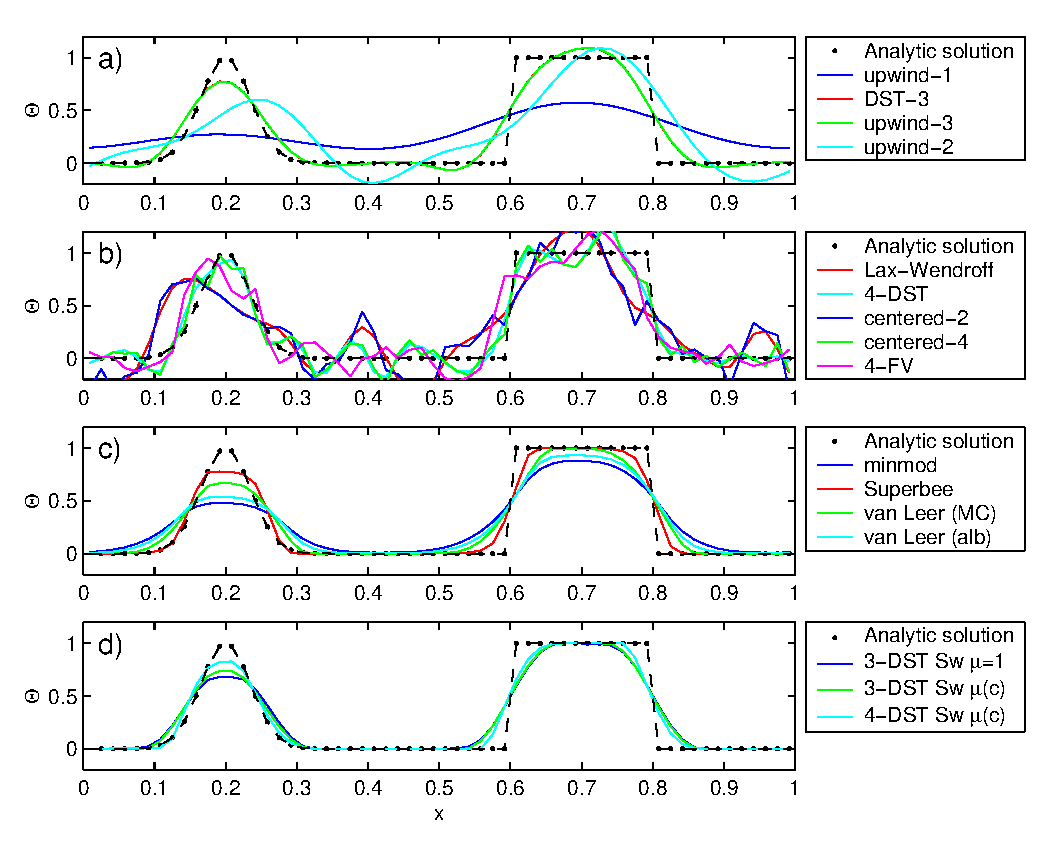
\includegraphics{part2/advect-1d-lo.eps}}
\caption{
Comparison of 1-D advection schemes. Courant number is 0.05 with 60
points and solutions are shown for T=1 (one complete period).
a) Shows the upwind biased schemes; first order upwind, DST3,
third order upwind and second order upwind.
b) Shows the centered schemes; Lax-Wendroff, DST4, centered second order,
centered fourth order and finite volume fourth order.
c) Shows the second order flux limiters: minmod, Superbee,
MC limiter and the van Leer limiter.
d) Shows the DST3 method with flux limiters due to Sweby with
$\mu=1$, $\mu=c/(1-c)$ and a fourth order DST method with Sweby limiter,
$\mu=c/(1-c)$.
\label{fig:advect-1d-lo}
}
\end{figure}

\begin{figure}
\resizebox{5.5in}{!}{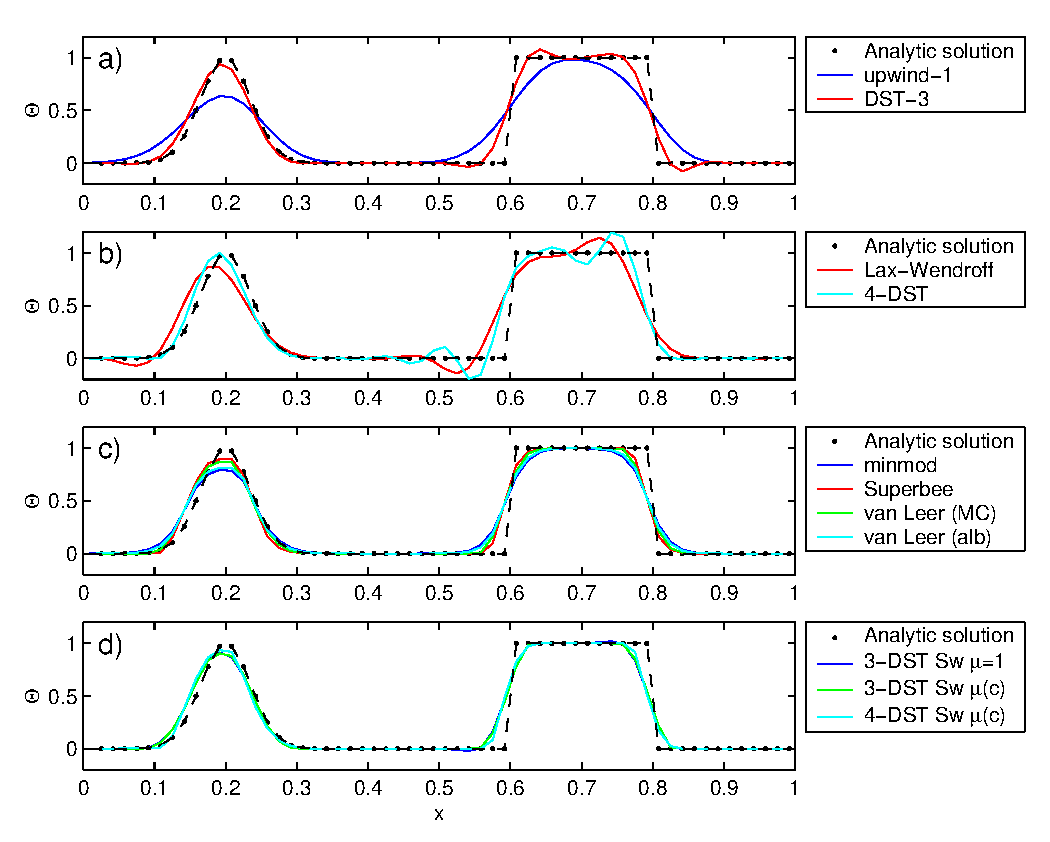
\includegraphics{part2/advect-1d-hi.eps}}
\caption{
Comparison of 1-D advection schemes. Courant number is 0.89 with 60
points and solutions are shown for T=1 (one complete period).
a) Shows the upwind biased schemes; first order upwind and DST3.
Third order upwind and second order upwind are unstable at this Courant number.
b) Shows the centered schemes; Lax-Wendroff, DST4. Centered second order,
centered fourth order and finite volume fourth order and unstable at this
Courant number.
c) Shows the second order flux limiters: minmod, Superbee,
MC limiter and the van Leer limiter.
d) Shows the DST3 method with flux limiters due to Sweby with
$\mu=1$, $\mu=c/(1-c)$ and a fourth order DST method with Sweby limiter,
$\mu=c/(1-c)$.
\label{fig:advect-1d-hi}
}
\end{figure}

The advection schemes known as centered second order, centered fourth
order, first order upwind and upwind biased third order are known as
linear advection schemes because the coefficient for interpolation of
the advected tracer are linear and a function only of the flow, not
the tracer field it self. We discuss these first since they are most
commonly used in the field and most familiar.

\subsection{Centered second order advection-diffusion}

The basic discretization, centered second order, is the default. It is
designed to be consistent with the continuity equation to facilitate
conservation properties analogous to the continuum. However, centered
second order advection is notoriously noisy and must be used in
conjunction with some finite amount of diffusion to produce a sensible
solution.

The advection operator is discretized:
\begin{equation}
{\cal A}_c \Delta r_f h_c G_{adv}^\tau = 
\delta_i F_x + \delta_j F_y + \delta_k F_r
\end{equation}
where the area integrated fluxes are given by:
\begin{eqnarray}
F_x & = & U \overline{ \tau }^i \\
F_y & = & V \overline{ \tau }^j \\
F_r & = & W \overline{ \tau }^k
\end{eqnarray}
The quantities $U$, $V$ and $W$ are volume fluxes defined:
\marginpar{$U$: {\bf uTrans} }
\marginpar{$V$: {\bf vTrans} }
\marginpar{$W$: {\bf rTrans} }
\begin{eqnarray}
U & = & \Delta y_g \Delta r_f h_w u \\
V & = & \Delta x_g \Delta r_f h_s v \\
W & = & {\cal A}_c w
\end{eqnarray}

For non-divergent flow, this discretization can be shown to conserve
the tracer both locally and globally and to globally conserve tracer
variance, $\tau^2$. The proof is given in \cite{adcroft:95,adcroft:97}.

\fbox{ \begin{minipage}{4.75in}
{\em S/R GAD\_C2\_ADV\_X} ({\em gad\_c2\_adv\_x.F})

$F_x$: {\bf uT} (argument)

$U$: {\bf uTrans} (argument)

$\tau$: {\bf tracer} (argument)

{\em S/R GAD\_C2\_ADV\_Y} ({\em gad\_c2\_adv\_y.F})

$F_y$: {\bf vT} (argument)

$V$: {\bf vTrans} (argument)

$\tau$: {\bf tracer} (argument)

{\em S/R GAD\_C2\_ADV\_R} ({\em gad\_c2\_adv\_r.F})

$F_r$: {\bf wT} (argument)

$W$: {\bf rTrans} (argument)

$\tau$: {\bf tracer} (argument)

\end{minipage} }


\subsection{Third order upwind bias advection}

Upwind biased third order advection offers a relatively good
compromise between accuracy and smoothness. It is not a ``positive''
scheme meaning false extrema are permitted but the amplitude of such
are significantly reduced over the centered second order method.

The third order upwind fluxes are discretized:
\begin{eqnarray}
F_x & = & U \overline{\tau - \frac{1}{6} \delta_{ii} \tau}^i
         + \frac{1}{2} |U| \delta_i \frac{1}{6} \delta_{ii} \tau \\
F_y & = & V \overline{\tau - \frac{1}{6} \delta_{ii} \tau}^j
         + \frac{1}{2} |V| \delta_j \frac{1}{6} \delta_{jj} \tau \\
F_r & = & W \overline{\tau - \frac{1}{6} \delta_{ii} \tau}^k
         + \frac{1}{2} |W| \delta_k \frac{1}{6} \delta_{kk} \tau 
\end{eqnarray}

At boundaries, $\delta_{\hat{n}} \tau$ is set to zero allowing
$\delta_{nn}$ to be evaluated. We are currently examine the accuracy
of this boundary condition and the effect on the solution.

\fbox{ \begin{minipage}{4.75in}
{\em S/R GAD\_U3\_ADV\_X} ({\em gad\_u3\_adv\_x.F})

$F_x$: {\bf uT} (argument)

$U$: {\bf uTrans} (argument)

$\tau$: {\bf tracer} (argument)

{\em S/R GAD\_U3\_ADV\_Y} ({\em gad\_u3\_adv\_y.F})

$F_y$: {\bf vT} (argument)

$V$: {\bf vTrans} (argument)

$\tau$: {\bf tracer} (argument)

{\em S/R GAD\_U3\_ADV\_R} ({\em gad\_u3\_adv\_r.F})

$F_r$: {\bf wT} (argument)

$W$: {\bf rTrans} (argument)

$\tau$: {\bf tracer} (argument)

\end{minipage} }

\subsection{Centered fourth order advection}

Centered fourth order advection is formally the most accurate scheme
we have implemented and can be used to great effect in high resolution
simulation where dynamical scales are well resolved. However, the
scheme is noisy like the centered second order method and so must be
used with some finite amount of diffusion. Bi-harmonic is recommended
since it is more scale selective and less likely to diffuse away the
well resolved gradient the fourth order scheme worked so hard to
create.

The centered fourth order fluxes are discretized:
\begin{eqnarray}
F_x & = & U \overline{\tau - \frac{1}{6} \delta_{ii} \tau}^i \\
F_y & = & V \overline{\tau - \frac{1}{6} \delta_{ii} \tau}^j \\
F_r & = & W \overline{\tau - \frac{1}{6} \delta_{ii} \tau}^k
\end{eqnarray}

As for the third order scheme, the best discretization near boundaries
is under investigation but currently $\delta_i \tau=0$ on a boundary.

\fbox{ \begin{minipage}{4.75in}
{\em S/R GAD\_C4\_ADV\_X} ({\em gad\_c4\_adv\_x.F})

$F_x$: {\bf uT} (argument)

$U$: {\bf uTrans} (argument)

$\tau$: {\bf tracer} (argument)

{\em S/R GAD\_C4\_ADV\_Y} ({\em gad\_c4\_adv\_y.F})

$F_y$: {\bf vT} (argument)

$V$: {\bf vTrans} (argument)

$\tau$: {\bf tracer} (argument)

{\em S/R GAD\_C4\_ADV\_R} ({\em gad\_c4\_adv\_r.F})

$F_r$: {\bf wT} (argument)

$W$: {\bf rTrans} (argument)

$\tau$: {\bf tracer} (argument)

\end{minipage} }


\subsection{First order upwind advection}

Although the upwind scheme is the underlying scheme for the robust or
non-linear methods given later, we haven't actually supplied this
method for general use. It would be very diffusive and it is unlikely
that it could ever produce more useful results than the positive
higher order schemes.

Upwind bias is introduced into many schemes using the {\em abs}
function and is allows the first order upwind flux to be written:
\begin{eqnarray}
F_x & = & U \overline{ \tau }^i - \frac{1}{2} |U| \delta_i \tau \\
F_y & = & V \overline{ \tau }^j - \frac{1}{2} |V| \delta_j \tau \\
F_r & = & W \overline{ \tau }^k - \frac{1}{2} |W| \delta_k \tau
\end{eqnarray}

If for some reason, the above method is required, then the second
order flux limiter scheme described later reduces to the above scheme
if the limiter is set to zero.


\section{Non-linear advection schemes}

Non-linear advection schemes invoke non-linear interpolation and are
widely used in computational fluid dynamics (non-linear does not refer
to the non-linearity of the advection operator). The flux limited
advection schemes belong to the class of finite volume methods which
neatly ties into the spatial discretization of the model.

When employing the flux limited schemes, first order upwind or
direct-space-time method the time-stepping is switched to forward in
time.

\subsection{Second order flux limiters}

The second order flux limiter method can be cast in several ways but
is generally expressed in terms of other flux approximations. For
example, in terms of a first order upwind flux and second order
Lax-Wendroff flux, the limited flux is given as:
\begin{equation}
F = F_1 + \psi(r) F_{LW}
\end{equation}
where $\psi(r)$ is the limiter function,
\begin{equation}
F_1 = u \overline{\tau}^i - \frac{1}{2} |u| \delta_i \tau
\end{equation}
is the upwind flux,
\begin{equation}
F_{LW} = F_1 + \frac{|u|}{2} (1-c) \delta_i \tau
\end{equation}
is the Lax-Wendroff flux and $c = \frac{u \Delta t}{\Delta x}$ is the
Courant (CFL) number.

The limiter function, $\psi(r)$, takes the slope ratio
\begin{eqnarray}
r = \frac{ \tau_{i-1} - \tau_{i-2} }{ \tau_{i} - \tau_{i-1} } & \forall & u > 0
\\
r = \frac{ \tau_{i+1} - \tau_{i} }{ \tau_{i} - \tau_{i-1} } & \forall & u < 0
\end{eqnarray}
as it's argument. There are many choices of limiter function but we
only provide the Superbee limiter \cite{roe:85}:
\begin{equation}
\psi(r) = \max[0,\min[1,2r],\min[2,r]]
\end{equation}

\fbox{ \begin{minipage}{4.75in}
{\em S/R GAD\_FLUXLIMIT\_ADV\_X} ({\em gad\_fluxlimit\_adv\_x.F})

$F_x$: {\bf uT} (argument)

$U$: {\bf uTrans} (argument)

$\tau$: {\bf tracer} (argument)

{\em S/R GAD\_FLUXLIMIT\_ADV\_Y} ({\em gad\_fluxlimit\_adv\_y.F})

$F_y$: {\bf vT} (argument)

$V$: {\bf vTrans} (argument)

$\tau$: {\bf tracer} (argument)

{\em S/R GAD\_FLUXLIMIT\_ADV\_R} ({\em gad\_fluxlimit\_adv\_r.F})

$F_r$: {\bf wT} (argument)

$W$: {\bf rTrans} (argument)

$\tau$: {\bf tracer} (argument)

\end{minipage} }


\subsection{Third order direct space time}

The direct-space-time method deals with space and time discretization
together (other methods that treat space and time separately are known
collectively as the ``Method of Lines''). The Lax-Wendroff scheme
falls into this category; it adds sufficient diffusion to a second
order flux that the forward-in-time method is stable. The upwind
biased third order DST scheme is:
\begin{eqnarray}
F = u \left( \tau_{i-1}
        + d_0 (\tau_{i}-\tau_{i-1}) + d_1 (\tau_{i-1}-\tau_{i-2}) \right)
& \forall & u > 0 \\
F = u \left( \tau_{i}
        - d_0 (\tau_{i}-\tau_{i-1}) - d_1 (\tau_{i+1}-\tau_{i}) \right)
& \forall & u < 0
\end{eqnarray}
where
\begin{eqnarray}
d_1 & = & \frac{1}{6} ( 2 - |c| ) ( 1 - |c| ) \\
d_2 & = & \frac{1}{6} ( 1 - |c| ) ( 1 + |c| )
\end{eqnarray}
The coefficients $d_0$ and $d_1$ approach $1/3$ and $1/6$ respectively
as the Courant number, $c$, vanishes. In this limit, the conventional
third order upwind method is recovered. For finite Courant number, the
deviations from the linear method are analogous to the diffusion added
to centered second order advection in the Lax-Wendroff scheme.

The DST3 method described above must be used in a forward-in-time
manner and is stable for $0 \le |c| \le 1$. Although the scheme
appears to be forward-in-time, it is in fact second order in time and
the accuracy increases with the Courant number! For low Courant
number, DST3 produces very similar results (indistinguishable in
Fig.~\ref{fig:advect-1d-lo}) to the linear third order method but for
large Courant number, where the linear upwind third order method is
unstable, the scheme is extremely accurate
(Fig.~\ref{fig:advect-1d-hi}) with only minor overshoots.

\fbox{ \begin{minipage}{4.75in}
{\em S/R GAD\_DST3\_ADV\_X} ({\em gad\_dst3\_adv\_x.F})

$F_x$: {\bf uT} (argument)

$U$: {\bf uTrans} (argument)

$\tau$: {\bf tracer} (argument)

{\em S/R GAD\_DST3\_ADV\_Y} ({\em gad\_dst3\_adv\_y.F})

$F_y$: {\bf vT} (argument)

$V$: {\bf vTrans} (argument)

$\tau$: {\bf tracer} (argument)

{\em S/R GAD\_DST3\_ADV\_R} ({\em gad\_dst3\_adv\_r.F})

$F_r$: {\bf wT} (argument)

$W$: {\bf rTrans} (argument)

$\tau$: {\bf tracer} (argument)

\end{minipage} }


\subsection{Third order direct space time with flux limiting}

The overshoots in the DST3 method can be controlled with a flux limiter.
The limited flux is written:
\begin{equation}
F =
\frac{1}{2}(u+|u|)\left( \tau_{i-1} + \psi(r^+)(\tau_{i} - \tau_{i-1} )\right)
+
\frac{1}{2}(u-|u|)\left( \tau_{i-1} + \psi(r^-)(\tau_{i} - \tau_{i-1} )\right)
\end{equation}
where
\begin{eqnarray}
r^+ & = & \frac{\tau_{i-1} - \tau_{i-2}}{\tau_{i} - \tau_{i-1}} \\
r^- & = & \frac{\tau_{i+1} - \tau_{i}}{\tau_{i} - \tau_{i-1}}
\end{eqnarray}
and the limiter is the Sweby limiter:
\begin{equation}
\psi(r) = \max[0, \min[\min(1,d_0+d_1r],\frac{1-c}{c}r ]]
\end{equation}

\fbox{ \begin{minipage}{4.75in}
{\em S/R GAD\_DST3FL\_ADV\_X} ({\em gad\_dst3\_adv\_x.F})

$F_x$: {\bf uT} (argument)

$U$: {\bf uTrans} (argument)

$\tau$: {\bf tracer} (argument)

{\em S/R GAD\_DST3FL\_ADV\_Y} ({\em gad\_dst3\_adv\_y.F})

$F_y$: {\bf vT} (argument)

$V$: {\bf vTrans} (argument)

$\tau$: {\bf tracer} (argument)

{\em S/R GAD\_DST3FL\_ADV\_R} ({\em gad\_dst3\_adv\_r.F})

$F_r$: {\bf wT} (argument)

$W$: {\bf rTrans} (argument)

$\tau$: {\bf tracer} (argument)

\end{minipage} }


\subsection{Multi-dimensional advection}

\begin{figure}
\resizebox{5.5in}{!}{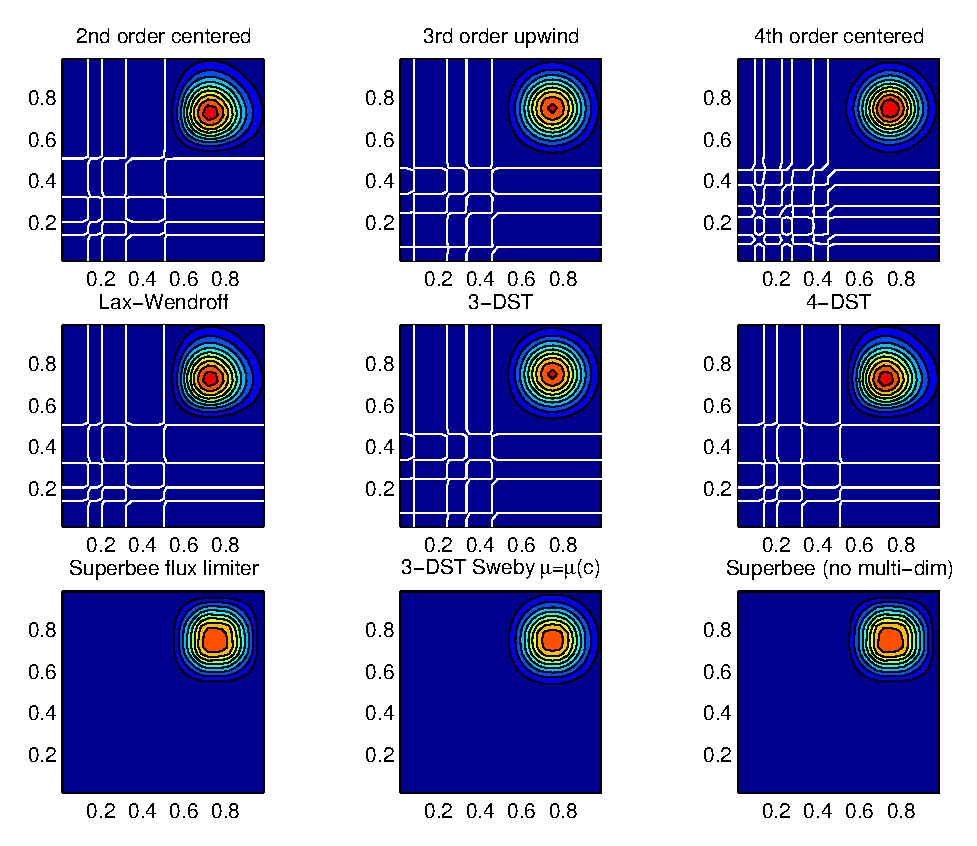
\includegraphics{part2/advect-2d-lo-diag.eps}}
\caption{
Comparison of advection schemes in two dimensions; diagonal advection
of a resolved Gaussian feature. Courant number is 0.01 with
30$\times$30 points and solutions are shown for T=1/2. White lines
indicate zero crossing (ie. the presence of false minima).  The left
column shows the second order schemes; top) centered second order with
Adams-Bashforth, middle) Lax-Wendroff and bottom) Superbee flux
limited. The middle column shows the third order schemes; top) upwind
biased third order with Adams-Bashforth, middle) third order direct
space-time method and bottom) the same with flux limiting. The top
right panel shows the centered fourth order scheme with
Adams-Bashforth and right middle panel shows a fourth order variant on
the DST method. Bottom right panel shows the Superbee flux limiter
(second order) applied independently in each direction (method of
lines).
\label{fig:advect-2d-lo-diag}
}
\end{figure}

\begin{figure}
\resizebox{5.5in}{!}{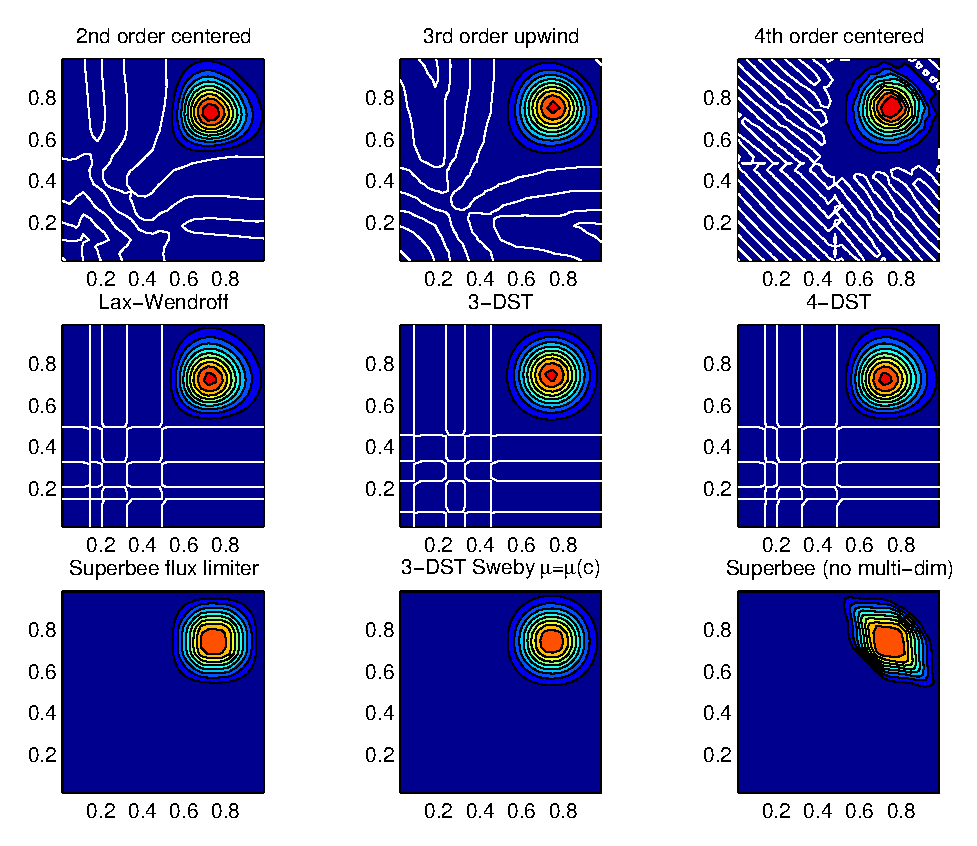
\includegraphics{part2/advect-2d-mid-diag.eps}}
\caption{
Comparison of advection schemes in two dimensions; diagonal advection
of a resolved Gaussian feature. Courant number is 0.27 with
30$\times$30 points and solutions are shown for T=1/2. White lines
indicate zero crossing (ie. the presence of false minima).  The left
column shows the second order schemes; top) centered second order with
Adams-Bashforth, middle) Lax-Wendroff and bottom) Superbee flux
limited. The middle column shows the third order schemes; top) upwind
biased third order with Adams-Bashforth, middle) third order direct
space-time method and bottom) the same with flux limiting. The top
right panel shows the centered fourth order scheme with
Adams-Bashforth and right middle panel shows a fourth order variant on
the DST method. Bottom right panel shows the Superbee flux limiter
(second order) applied independently in each direction (method of
lines).
\label{fig:advect-2d-mid-diag}
}
\end{figure}

\begin{figure}
\resizebox{5.5in}{!}{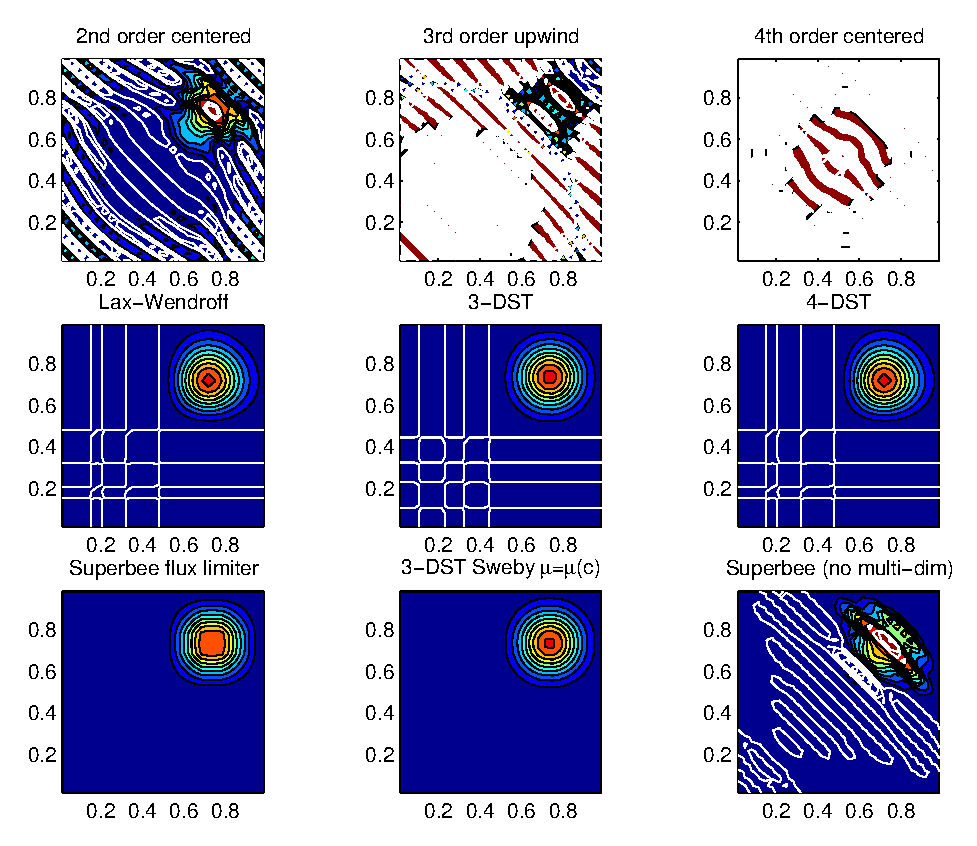
\includegraphics{part2/advect-2d-hi-diag.eps}}
\caption{
Comparison of advection schemes in two dimensions; diagonal advection
of a resolved Gaussian feature. Courant number is 0.47 with
30$\times$30 points and solutions are shown for T=1/2. White lines
indicate zero crossings and initial maximum values (ie. the presence
of false extrema).  The left column shows the second order schemes;
top) centered second order with Adams-Bashforth, middle) Lax-Wendroff
and bottom) Superbee flux limited. The middle column shows the third
order schemes; top) upwind biased third order with Adams-Bashforth,
middle) third order direct space-time method and bottom) the same with
flux limiting. The top right panel shows the centered fourth order
scheme with Adams-Bashforth and right middle panel shows a fourth
order variant on the DST method. Bottom right panel shows the Superbee
flux limiter (second order) applied independently in each direction
(method of lines).
\label{fig:advect-2d-hi-diag}
}
\end{figure}



In many of the aforementioned advection schemes the behavior in
multiple dimensions is not necessarily as good as the one dimensional
behavior. For instance, a shape preserving monotonic scheme in one
dimension can have severe shape distortion in two dimensions if the
two components of horizontal fluxes are treated independently. There
is a large body of literature on the subject dealing with this problem
and among the fixes are operator and flux splitting methods, corner
flux methods and more. We have adopted a variant on the standard
splitting methods that allows the flux calculations to be implemented
as if in one dimension:
\begin{eqnarray}
\tau^{n+1/3} & = & \tau^{n}
- \Delta t \left( \frac{1}{\Delta x} \delta_i F^x(\tau^{n})
           + \tau^{n} \frac{1}{\Delta x} \delta_i u \right) \\
\tau^{n+2/3} & = & \tau^{n}
- \Delta t \left( \frac{1}{\Delta y} \delta_j F^y(\tau^{n+1/3})
           + \tau^{n} \frac{1}{\Delta y} \delta_i v \right) \\
\tau^{n+3/3} & = & \tau^{n}
- \Delta t \left( \frac{1}{\Delta r} \delta_k F^x(\tau^{n+2/3})
           + \tau^{n} \frac{1}{\Delta r} \delta_i w \right)
\end{eqnarray}

In order to incorporate this method into the general model algorithm,
we compute the effective tendency rather than update the tracer so
that other terms such as diffusion are using the $n$ time-level and
not the updated $n+3/3$ quantities:
\begin{equation}
G^{n+1/2}_{adv} = \frac{1}{\Delta t} ( \tau^{n+3/3} - \tau^{n} )
\end{equation}
So that the over all time-stepping looks likes:
\begin{equation}
\tau^{n+1} = \tau^{n} + \Delta t \left( G^{n+1/2}_{adv} + G_{diff}(\tau^{n}) + G^{n}_{forcing} \right)
\end{equation}

\fbox{ \begin{minipage}{4.75in}
{\em S/R GAD\_ADVECTION} ({\em gad\_advection.F})

$\tau$: {\bf Tracer} (argument)

$G^{n+1/2}_{adv}$: {\bf Gtracer} (argument)

$F_x, F_y, F_r$: {\bf af} (local)

$U$: {\bf uTrans} (local)

$V$: {\bf vTrans} (local)

$W$: {\bf rTrans} (local)

\end{minipage} }


\section{Comparison of advection schemes}

Figs.~\ref{fig:advect-2d-lo-diag}, \ref{fig:advect-2d-mid-diag} and
\ref{fig:advect-2d-hi-diag} show solutions to a simple diagonal
advection problem using a selection of schemes for low, moderate and
high Courant numbers, respectively. The top row shows the linear
schemes, integrated with the Adams-Bashforth method. Theses schemes
are clearly unstable for the high Courant number and weakly unstable
for the moderate Courant number. The presence of false extrema is very
apparent for all Courant numbers. The middle row shows solutions
obtained with the unlimited but multi-dimensional schemes. These
solutions also exhibit false extrema though the pattern now shows
symmetry due to the multi-dimensional scheme. Also, the schemes are
stable at high Courant number where the linear schemes weren't. The
bottom row (left and middle) shows the limited schemes and most
obvious is the absence of false extrema. The accuracy and stability of
the unlimited non-linear schemes is retained at high Courant number
but at low Courant number the tendency is to loose amplitude in sharp
peaks due to diffusion. The one dimensional tests shown in
Figs.~\ref{fig:advect-1d-lo} and \ref{fig:advect-1d-hi} showed this
phenomenon.

Finally, the bottom left and right panels use the same advection
scheme but the right does not use the multi-dimensional method. At low
Courant number this appears to not matter but for moderate Courant
number severe distortion of the feature is apparent. Moreover, the
stability of the multi-dimensional scheme is determined by the maximum
Courant number applied of each dimension while the stability of the
method of lines is determined by the sum. Hence, in the high Courant
number plot, the scheme is unstable.

With many advection schemes implemented in the code two questions
arise: ``Which scheme is best?'' and ``Why don't you just offer the
best advection scheme?''. Unfortunately, no one advection scheme is
``the best'' for all particular applications and for new applications
it is often a matter of trial to determine which is most
suitable. Here are some guidelines but these are not the rule;
\begin{itemize}
\item If you have a coarsely resolved model, using a
positive or upwind biased scheme will introduce significant diffusion
to the solution and using a centered higher order scheme will
introduce more noise. In this case, simplest may be best.
\item If you have a high resolution model, using a higher order
scheme will give a more accurate solution but scale-selective
diffusion might need to be employed. The flux limited methods
offer similar accuracy in this regime.
\item If your solution has shocks or propagating fronts then a
flux limited scheme is almost essential.
\item If your time-step is limited by advection, the multi-dimensional
non-linear schemes have the most stability (up to Courant number 1).
\item If you need to know how much diffusion/dissipation has occurred you
will have a lot of trouble figuring it out with a non-linear method.
\item The presence of false extrema is non-physical and this alone is the
strongest argument for using a positive scheme.
\end{itemize}

% $Header: /u/gcmpack/manual/s_algorithm/text/shap.tex,v 1.2 2001/08/09 19:48:39 adcroft Exp $
% $Name:  $

\section{Shapiro Filter} 

The Shapiro filter (Shapiro 1970, 1975) is a high order horizontal 
filter that efficiently remove small scale grid noise 
without affecting the physical structures of a field. 
It is applied at the end of the time step %(the\_correction\_step),
on both velocity and tracer fields.

Three different space operators are considered here (S1,S2 and S4).
They differs essentially by the sequence of derivative in
both X and Y directions. Consequently they show different 
damping response function specially in the diagonal directions 
X+Y and X-Y.

Space derivatives can be computed in the real space, 
taken into account the grid spacing. 
Alternatively, a pure computational filter can be defined,
using pure numerical differences and ignoring 
grid spacing. 
This later form is stable whatever the grid is, and therefore
specially useful for highly anisotrope grid such as spherical 
coordinate grid.
A damping time-scale parameter $\tau_{shap}$ 
defines the strength of the filter damping.

The 3 computational filter operators are :
$$
\mathrm{S1c:}\hspace{2cm}
[1 - 1/2 \frac{\Delta t}{\tau_{shap}}
   \{ (\frac{1}{4}\delta_{ii})^n 
    + (\frac{1}{4}\delta_{jj})^n \} ] 
$$

$$
\mathrm{S2c:}\hspace{2cm}
[1 - \frac{\Delta t}{\tau_{shap}} 
\{ \frac{1}{8} (\delta_{ii} + \delta_{jj}) \}^n]
$$

$$
\mathrm{S4c:}\hspace{2cm}
[1 - \frac{\Delta t}{\tau_{shap}} (\frac{1}{4}\delta_{ii})^n]
[1 - \frac{\Delta t}{\tau_{shap}} (\frac{1}{4}\delta_{jj})^n]
$$

In addition, the S2 operator can easly be extended to 
a physical space filter: 
$$
\mathrm{S2g:}\hspace{2cm}
[1 - \frac{\Delta t}{\tau_{shap}} 
\{ \frac{L_{shap}^2}{8} \overline{\nabla}^2 \}^n]
$$

with the Laplacien operator $\overline{\nabla}^2 $
and a length scale parameter $L_{shap}$.
The stability of this S2g filter requires 
$L_{shap} < \mathrm{Min}^{(Global)}(\Delta x,\Delta y)$.

\marginpar{Add Response functions and figures}


%\pagebreak

% Section: Getting started
% $Header: /u/gcmpack/manual/s_getstarted/text/top_section.tex,v 1.3 2001/12/19 14:34:39 helen Exp $
% $Name:  $

\chapter{Getting started and using the MITgcm}

% $Header: /u/gcmpack/manual/s_getstarted/text/getting_started.tex,v 1.40 2010/01/21 19:20:08 jmc Exp $
% $Name:  $

%\section{Getting started}

We believe the best way to familiarize yourself with the
model is to run the case study examples provided with the base
version. Information on how to obtain, compile, and run the code is
found here as well as a brief description of the model structure
directory and the case study examples. Information is also provided
here on how to customize the code when you are ready to try implementing 
the configuration you have in mind.  The code and algorithm
are described more fully in chapters \ref{chap:discretization} and 
\ref{chap:sarch}. 

\section{Where to find information}
\label{sect:whereToFindInfo}
\begin{rawhtml}
<!-- CMIREDIR:whereToFindInfo: -->
\end{rawhtml}

There is a web-archived support mailing list for the model that
you can email at \texttt{MITgcm-support@mitgcm.org} or browse at:
\begin{rawhtml} <A href=http://mitgcm.org/mailman/listinfo/mitgcm-support/ target="idontexist"> \end{rawhtml}
\begin{verbatim}
http://mitgcm.org/mailman/listinfo/mitgcm-support/
http://mitgcm.org/pipermail/mitgcm-support/
\end{verbatim}
\begin{rawhtml} </A> \end{rawhtml}

\section{Obtaining the code}
\label{sect:obtainingCode}
\begin{rawhtml}
<!-- CMIREDIR:obtainingCode: -->
\end{rawhtml}

MITgcm can be downloaded from our system by following
the instructions below. As a courtesy we ask that you send e-mail to us at
\begin{rawhtml} <A href=mailto:MITgcm-support@mitgcm.org> \end{rawhtml}
MITgcm-support@mitgcm.org
\begin{rawhtml} </A> \end{rawhtml}
to enable us to keep track of who's using the model and in what application.
You can download the model two ways:

\begin{enumerate}
\item Using CVS software. CVS is a freely available source code management
tool. To use CVS you need to have the software installed. Many systems
come with CVS pre-installed, otherwise good places to look for
the software for a particular platform are
\begin{rawhtml} <A href=http://www.cvshome.org/ target="idontexist"> \end{rawhtml}
cvshome.org
\begin{rawhtml} </A> \end{rawhtml}
and
\begin{rawhtml} <A href=http://www.wincvs.org/ target="idontexist"> \end{rawhtml}
wincvs.org
\begin{rawhtml} </A> \end{rawhtml}
.

\item Using a tar file. This method is simple and does not
require any special software. However, this method does not
provide easy support for maintenance updates.

\end{enumerate}

\subsection{Method 1 - Checkout from CVS}
\label{sect:cvs_checkout}

If CVS is available on your system, we strongly encourage you to use it. CVS
provides an efficient and elegant way of organizing your code and keeping
track of your changes. If CVS is not available on your machine, you can also
download a tar file.

Before you can use CVS, the following environment variable(s) should
be set within your shell.  For a csh or tcsh shell, put the following 
\begin{verbatim}
% setenv CVSROOT :pserver:cvsanon@mitgcm.org:/u/gcmpack
\end{verbatim}
in your \texttt{.cshrc} or \texttt{.tcshrc} file.  For bash or sh
shells, put:
\begin{verbatim}
% export CVSROOT=':pserver:cvsanon@mitgcm.org:/u/gcmpack'
\end{verbatim}
in your \texttt{.profile} or \texttt{.bashrc} file.


To get MITgcm through CVS, first register with the MITgcm CVS server
using command:
\begin{verbatim}
% cvs login ( CVS password: cvsanon )
\end{verbatim}
You only need to do a ``cvs login'' once.

To obtain the latest sources type:
\begin{verbatim}
% cvs co MITgcm
\end{verbatim}
or to get a specific release type:
\begin{verbatim}
% cvs co -P -r checkpoint52i_post  MITgcm
\end{verbatim}
The MITgcm web site contains further directions concerning the source
code and CVS.  It also contains a web interface to our CVS archive so
that one may easily view the state of files, revisions, and other
development milestones:
%\begin{rawhtml} <A href="http://mitgcm.org/download" target="idontexist"> \end{rawhtml}
\begin{rawhtml} <A href="http://mitgcm.org/viewvc/MITgcm/MITgcm/" target="idontexist"> \end{rawhtml}
\begin{verbatim}
http://mitgcm.org/source_code.html
\end{verbatim}
\begin{rawhtml} </A> \end{rawhtml}

As a convenience, the MITgcm CVS server contains aliases which are
named subsets of the codebase.  These aliases can be especially
helpful when used over slow internet connections or on machines with
restricted storage space.  Table \ref{tab:cvsModules} contains a list
of CVS aliases
\begin{table}[htb]
  \centering
  \begin{tabular}[htb]{|lp{3.25in}|}\hline
    \textbf{Alias Name}    &  \textbf{Information (directories) Contained}  \\\hline
    \texttt{MITgcm\_code}  &  Only the source code -- none of the verification examples.  \\
    \texttt{MITgcm\_verif\_basic}
    &  Source code plus a small set of the verification examples 
    (\texttt{global\_ocean.90x40x15}, \texttt{aim.5l\_cs}, \texttt{hs94.128x64x5}, 
    \texttt{front\_relax}, and \texttt{plume\_on\_slope}).  \\
    \texttt{MITgcm\_verif\_atmos}  &  Source code plus all of the atmospheric examples.  \\
    \texttt{MITgcm\_verif\_ocean}  &  Source code plus all of the oceanic examples.  \\
    \texttt{MITgcm\_verif\_all}    &  Source code plus all of the
    verification examples. \\\hline
  \end{tabular}
  \caption{MITgcm CVS Modules}
  \label{tab:cvsModules}
\end{table}

The checkout process creates a directory called \texttt{MITgcm}. If
the directory \texttt{MITgcm} exists this command updates your code
based on the repository. Each directory in the source tree contains a
directory \texttt{CVS}. This information is required by CVS to keep
track of your file versions with respect to the repository. Don't edit
the files in \texttt{CVS}!  You can also use CVS to download code
updates.  More extensive information on using CVS for maintaining
MITgcm code can be found
\begin{rawhtml} <A href="http://mitgcm.org/usingcvstoget.html" target="idontexist"> \end{rawhtml}
here
\begin{rawhtml} </A> \end{rawhtml} 
.
It is important to note that the CVS aliases in Table
\ref{tab:cvsModules} cannot be used in conjunction with the CVS
\texttt{-d DIRNAME} option.  However, the \texttt{MITgcm} directories
they create can be changed to a different name following the check-out:
\begin{verbatim}
   %  cvs co MITgcm_verif_basic
   %  mv MITgcm MITgcm_verif_basic
\end{verbatim}

\subsubsection{Upgrading from an earlier version}

If you already have an earlier version of the code you can ``upgrade''
your copy instead of downloading the entire repository again. First,
``cd'' (change directory) to the top of your working copy:
\begin{verbatim}
% cd MITgcm
\end{verbatim}
and then issue the cvs update command such as:
\begin{verbatim}
% cvs -q update -r checkpoint52i_post -d -P
\end{verbatim}
This will update the ``tag'' to ``checkpoint52i\_post'', add any new
directories (-d) and remove any empty directories (-P). The -q option
means be quiet which will reduce the number of messages you'll see in
the terminal. If you have modified the code prior to upgrading, CVS
will try to merge your changes with the upgrades. If there is a
conflict between your modifications and the upgrade, it will report
that file with a ``C'' in front, e.g.:
\begin{verbatim}
C model/src/ini_parms.F
\end{verbatim}
If the list of conflicts scrolled off the screen, you can re-issue the
cvs update command and it will report the conflicts. Conflicts are
indicated in the code by the delimites ``$<<<<<<<$'', ``======='' and
``$>>>>>>>$''. For example,
{\small
\begin{verbatim}
<<<<<<< ini_parms.F
     & bottomDragLinear,myOwnBottomDragCoefficient,
=======
     & bottomDragLinear,bottomDragQuadratic,
>>>>>>> 1.18
\end{verbatim}
}
means that you added ``myOwnBottomDragCoefficient'' to a namelist at
the same time and place that we added ``bottomDragQuadratic''. You
need to resolve this conflict and in this case the line should be
changed to:
{\small
\begin{verbatim}
     & bottomDragLinear,bottomDragQuadratic,myOwnBottomDragCoefficient,
\end{verbatim}
}
and the lines with the delimiters ($<<<<<<$,======,$>>>>>>$) be deleted.
Unless you are making modifications which exactly parallel
developments we make, these types of conflicts should be rare.

\paragraph*{Upgrading to the current pre-release version}

We don't make a ``release'' for every little patch and bug fix in
order to keep the frequency of upgrades to a minimum. However, if you
have run into a problem for which ``we have already fixed in the
latest code'' and we haven't made a ``tag'' or ``release'' since that
patch then you'll need to get the latest code:
\begin{verbatim}
% cvs -q update -A -d -P
\end{verbatim}
Unlike, the ``check-out'' and ``update'' procedures above, there is no
``tag'' or release name. The -A tells CVS to upgrade to the
very latest version. As a rule, we don't recommend this since you
might upgrade while we are in the processes of checking in the code so
that you may only have part of a patch. Using this method of updating
also means we can't tell what version of the code you are working
with. So please be sure you understand what you're doing.

\subsection{Method 2 - Tar file download}
\label{sect:conventionalDownload}

If you do not have CVS on your system, you can download the model as a
tar file from the web site at:
\begin{rawhtml} <A href=http://mitgcm.org/download/ target="idontexist"> \end{rawhtml}
\begin{verbatim}
http://mitgcm.org/download/
\end{verbatim}
\begin{rawhtml} </A> \end{rawhtml}
The tar file still contains CVS information which we urge you not to
delete; even if you do not use CVS yourself the information can help
us if you should need to send us your copy of the code.  If a recent
tar file does not exist, then please contact the developers through
the 
\begin{rawhtml} <A href="mailto:MITgcm-support@mitgcm.org"> \end{rawhtml}
MITgcm-support@mitgcm.org
\begin{rawhtml} </A> \end{rawhtml}
mailing list.

\section{Model and directory structure}
\begin{rawhtml}
<!-- CMIREDIR:directory_structure: -->
\end{rawhtml}

The ``numerical'' model is contained within a execution environment
support wrapper. This wrapper is designed to provide a general
framework for grid-point models. MITgcmUV is a specific numerical
model that uses the framework. Under this structure the model is split
into execution environment support code and conventional numerical
model code. The execution environment support code is held under the
\texttt{eesupp} directory. The grid point model code is held under the
\texttt{model} directory. Code execution actually starts in the
\texttt{eesupp} routines and not in the \texttt{model} routines. For
this reason the top-level \texttt{MAIN.F} is in the
\texttt{eesupp/src} directory. In general, end-users should not need
to worry about this level. The top-level routine for the numerical
part of the code is in \texttt{model/src/THE\_MODEL\_MAIN.F}. Here is
a brief description of the directory structure of the model under the
root tree (a detailed description is given in section 3: Code
structure).

\begin{itemize}

\item \texttt{doc}: contains brief documentation notes.
  
\item \texttt{eesupp}: contains the execution environment source code.
  Also subdivided into two subdirectories \texttt{inc} and
  \texttt{src}.
  
\item \texttt{model}: this directory contains the main source code.
  Also subdivided into two subdirectories \texttt{inc} and
  \texttt{src}.
  
\item \texttt{pkg}: contains the source code for the packages. Each
  package corresponds to a subdirectory. For example, \texttt{gmredi}
  contains the code related to the Gent-McWilliams/Redi scheme,
  \texttt{aim} the code relative to the atmospheric intermediate
  physics. The packages are described in detail in chapter \ref{chap.packagesI}.
  
\item \texttt{tools}: this directory contains various useful tools.
  For example, \texttt{genmake2} is a script written in csh (C-shell)
  that should be used to generate your makefile. The directory
  \texttt{adjoint} contains the makefile specific to the Tangent
  linear and Adjoint Compiler (TAMC) that generates the adjoint code.
  The latter is described in detail in part \ref{chap.ecco}.
  This directory also contains the subdirectory build\_options, which
  contains the `optfiles' with the compiler options for the different
  compilers and machines that can run MITgcm.
  
\item \texttt{utils}: this directory contains various utilities. The
  subdirectory \texttt{knudsen2} contains code and a makefile that
  compute coefficients of the polynomial approximation to the knudsen
  formula for an ocean nonlinear equation of state. The
  \texttt{matlab} subdirectory contains matlab scripts for reading
  model output directly into matlab. \texttt{scripts} contains C-shell
  post-processing scripts for joining processor-based and tiled-based
  model output. The subdirectory exch2 contains the code needed for
  the exch2 package to work with different combinations of domain
  decompositions.
  
\item \texttt{verification}: this directory contains the model
  examples. See section \ref{sect:modelExamples}.

\item \texttt{jobs}: contains sample job scripts for running MITgcm.
  
\item \texttt{lsopt}: Line search code used for optimization.
  
\item \texttt{optim}: Interface between MITgcm and line search code.
  
\end{itemize}

\section[Building MITgcm]{Building the code}
\label{sect:buildingCode}
\begin{rawhtml}
<!-- CMIREDIR:buildingCode: -->
\end{rawhtml}

To compile the code, we use the \texttt{make} program. This uses a
file (\texttt{Makefile}) that allows us to pre-process source files,
specify compiler and optimization options and also figures out any
file dependencies. We supply a script (\texttt{genmake2}), described
in section \ref{sect:genmake}, that automatically creates the
\texttt{Makefile} for you. You then need to build the dependencies and
compile the code.

As an example, assume that you want to build and run experiment
\texttt{verification/exp2}. The are multiple ways and places to
actually do this but here let's build the code in
\texttt{verification/exp2/build}:
\begin{verbatim}
% cd verification/exp2/build
\end{verbatim}
First, build the \texttt{Makefile}:
\begin{verbatim}
% ../../../tools/genmake2 -mods=../code
\end{verbatim}
The command line option tells \texttt{genmake} to override model source
code with any files in the directory \texttt{../code/}.

On many systems, the \texttt{genmake2} program will be able to
automatically recognize the hardware, find compilers and other tools
within the user's path (``\texttt{echo \$PATH}''), and then choose an
appropriate set of options from the files (``optfiles'') contained in
the \texttt{tools/build\_options} directory.  Under some
circumstances, a user may have to create a new ``optfile'' in order to
specify the exact combination of compiler, compiler flags, libraries,
and other options necessary to build a particular configuration of
MITgcm.  In such cases, it is generally helpful to read the existing
``optfiles'' and mimic their syntax.

Through the MITgcm-support list, the MITgcm developers are willing to
provide help writing or modifing ``optfiles''.  And we encourage users
to post new ``optfiles'' (particularly ones for new machines or
architectures) to the 
\begin{rawhtml} <A href="mailto:MITgcm-support@mitgcm.org"> \end{rawhtml}
MITgcm-support@mitgcm.org
\begin{rawhtml} </A> \end{rawhtml}
list.

To specify an optfile to \texttt{genmake2}, the syntax is:
\begin{verbatim}
% ../../../tools/genmake2 -mods=../code -of /path/to/optfile
\end{verbatim}

Once a \texttt{Makefile} has been generated, we create the
dependencies with the command:
\begin{verbatim}
% make depend
\end{verbatim}
This modifies the \texttt{Makefile} by attaching a (usually, long)
list of files upon which other files depend. The purpose of this is to
reduce re-compilation if and when you start to modify the code. The
{\tt make depend} command also creates links from the model source to
this directory.  It is important to note that the {\tt make depend}
stage will occasionally produce warnings or errors since the
dependency parsing tool is unable to find all of the necessary header
files (\textit{eg.}  \texttt{netcdf.inc}).  In these circumstances, it
is usually OK to ignore the warnings/errors and proceed to the next
step.

Next one can compile the code using:
\begin{verbatim}
% make
\end{verbatim}
The {\tt make} command creates an executable called \texttt{mitgcmuv}.
Additional make ``targets'' are defined within the makefile to aid in
the production of adjoint and other versions of MITgcm.  On SMP
(shared multi-processor) systems, the build process can often be sped
up appreciably using the command:
\begin{verbatim}
% make -j 2
\end{verbatim}
where the ``2'' can be replaced with a number that corresponds to the
number of CPUs available.

Now you are ready to run the model. General instructions for doing so are
given in section \ref{sect:runModel}. Here, we can run the model by
first creating links to all the input files:
\begin{verbatim}
ln -s ../input/* .
\end{verbatim}
and then calling the executable with:
\begin{verbatim}
./mitgcmuv > output.txt
\end{verbatim}
where we are re-directing the stream of text output to the file
\texttt{output.txt}.

\subsection{Building/compiling the code elsewhere}

In the example above (section \ref{sect:buildingCode}) we built the
executable in the {\em input} directory of the experiment for
convenience. You can also configure and compile the code in other
locations, for example on a scratch disk with out having to copy the
entire source tree. The only requirement to do so is you have {\tt
  genmake2} in your path or you know the absolute path to {\tt
  genmake2}.

The following sections outline some possible methods of organizing
your source and data.

\subsubsection{Building from the {\em ../code directory}}

This is just as simple as building in the {\em input/} directory:
\begin{verbatim}
% cd verification/exp2/code
% ../../../tools/genmake2
% make depend
% make
\end{verbatim}
However, to run the model the executable ({\em mitgcmuv}) and input
files must be in the same place. If you only have one calculation to make:
\begin{verbatim}
% cd ../input
% cp ../code/mitgcmuv ./
% ./mitgcmuv > output.txt
\end{verbatim}
or if you will be making multiple runs with the same executable:
\begin{verbatim}
% cd ../
% cp -r input run1
% cp code/mitgcmuv run1
% cd run1
% ./mitgcmuv > output.txt
\end{verbatim}

\subsubsection{Building from a new directory}

Since the {\em input} directory contains input files it is often more
useful to keep {\em input} pristine and build in a new directory
within {\em verification/exp2/}:
\begin{verbatim}
% cd verification/exp2
% mkdir build
% cd build
% ../../../tools/genmake2 -mods=../code
% make depend
% make
\end{verbatim}
This builds the code exactly as before but this time you need to copy
either the executable or the input files or both in order to run the
model. For example,
\begin{verbatim}
% cp ../input/* ./
% ./mitgcmuv > output.txt
\end{verbatim}
or if you tend to make multiple runs with the same executable then
running in a new directory each time might be more appropriate:
\begin{verbatim}
% cd ../
% mkdir run1
% cp build/mitgcmuv run1/
% cp input/* run1/
% cd run1
% ./mitgcmuv > output.txt
\end{verbatim}

\subsubsection{Building on a scratch disk}

Model object files and output data can use up large amounts of disk
space so it is often the case that you will be operating on a large
scratch disk. Assuming the model source is in {\em ~/MITgcm} then the
following commands will build the model in {\em /scratch/exp2-run1}:
\begin{verbatim}
% cd /scratch/exp2-run1
% ~/MITgcm/tools/genmake2 -rootdir=~/MITgcm \
  -mods=~/MITgcm/verification/exp2/code
% make depend
% make
\end{verbatim}
To run the model here, you'll need the input files:
\begin{verbatim}
% cp ~/MITgcm/verification/exp2/input/* ./
% ./mitgcmuv > output.txt
\end{verbatim}

As before, you could build in one directory and make multiple runs of
the one experiment:
\begin{verbatim}
% cd /scratch/exp2
% mkdir build
% cd build
% ~/MITgcm/tools/genmake2 -rootdir=~/MITgcm \
  -mods=~/MITgcm/verification/exp2/code
% make depend
% make
% cd ../
% cp -r ~/MITgcm/verification/exp2/input run2
% cd run2
% ./mitgcmuv > output.txt
\end{verbatim}


\subsection{Using \texttt{genmake2}}
\label{sect:genmake}

To compile the code, first use the program \texttt{genmake2} (located
in the \texttt{tools} directory) to generate a Makefile.
\texttt{genmake2} is a shell script written to work with all
``sh''--compatible shells including bash v1, bash v2, and Bourne.
Internally, \texttt{genmake2} determines the locations of needed
files, the compiler, compiler options, libraries, and Unix tools.  It
relies upon a number of ``optfiles'' located in the
\texttt{tools/build\_options} directory.

The purpose of the optfiles is to provide all the compilation options
for particular ``platforms'' (where ``platform'' roughly means the
combination of the hardware and the compiler) and code configurations.
Given the combinations of possible compilers and library dependencies
({\it eg.}  MPI and NetCDF) there may be numerous optfiles available
for a single machine.  The naming scheme for the majority of the
optfiles shipped with the code is
\begin{center}
  {\bf OS\_HARDWARE\_COMPILER }
\end{center}
where
\begin{description}
\item[OS] is the name of the operating system (generally the
  lower-case output of the {\tt 'uname'} command)
\item[HARDWARE] is a string that describes the CPU type and
  corresponds to output from the  {\tt 'uname -m'} command:
  \begin{description}
  \item[ia32] is for ``x86'' machines such as i386, i486, i586, i686,
    and athlon
  \item[ia64] is for Intel IA64 systems (eg. Itanium, Itanium2)
  \item[amd64] is AMD x86\_64 systems
  \item[ppc] is for Mac PowerPC systems
  \end{description}
\item[COMPILER] is the compiler name (generally, the name of the
  FORTRAN executable)
\end{description}

In many cases, the default optfiles are sufficient and will result in
usable Makefiles.  However, for some machines or code configurations,
new ``optfiles'' must be written. To create a new optfile, it is
generally best to start with one of the defaults and modify it to suit
your needs.  Like \texttt{genmake2}, the optfiles are all written
using a simple ``sh''--compatible syntax.  While nearly all variables
used within \texttt{genmake2} may be specified in the optfiles, the
critical ones that should be defined are:

\begin{description}
\item[FC] the FORTRAN compiler (executable) to use
\item[DEFINES] the command-line DEFINE options passed to the compiler
\item[CPP] the C pre-processor to use
\item[NOOPTFLAGS] options flags for special files that should not be
  optimized
\end{description}

For example, the optfile for a typical Red Hat Linux machine (``ia32''
architecture) using the GCC (g77) compiler is
\begin{verbatim}
FC=g77
DEFINES='-D_BYTESWAPIO -DWORDLENGTH=4'
CPP='cpp  -traditional -P'
NOOPTFLAGS='-O0'
#  For IEEE, use the "-ffloat-store" option
if test "x$IEEE" = x ; then
    FFLAGS='-Wimplicit -Wunused -Wuninitialized'
    FOPTIM='-O3 -malign-double -funroll-loops'
else
    FFLAGS='-Wimplicit -Wunused -ffloat-store'
    FOPTIM='-O0 -malign-double'
fi
\end{verbatim}

If you write an optfile for an unrepresented machine or compiler, you
are strongly encouraged to submit the optfile to the MITgcm project
for inclusion.  Please send the file to the
\begin{rawhtml} <A href="mail-to:MITgcm-support@mitgcm.org"> \end{rawhtml}
\begin{center}
  MITgcm-support@mitgcm.org
\end{center}
\begin{rawhtml} </A> \end{rawhtml}
mailing list.

In addition to the optfiles, \texttt{genmake2} supports a number of
helpful command-line options.  A complete list of these options can be
obtained from:
\begin{verbatim}
% genmake2 -h
\end{verbatim}

The most important command-line options are:
\begin{description}
  
\item[\texttt{--optfile=/PATH/FILENAME}] specifies the optfile that
  should be used for a particular build.
  
  If no "optfile" is specified (either through the command line or the
  MITGCM\_OPTFILE environment variable), genmake2 will try to make a
  reasonable guess from the list provided in {\em
    tools/build\_options}.  The method used for making this guess is
  to first determine the combination of operating system and hardware
  (eg. "linux\_ia32") and then find a working FORTRAN compiler within
  the user's path.  When these three items have been identified,
  genmake2 will try to find an optfile that has a matching name.
  
\item[\texttt{--pdefault='PKG1 PKG2 PKG3 ...'}] specifies the default
  set of packages to be used.  The normal order of precedence for
  packages is as follows:
  \begin{enumerate}
  \item If available, the command line (\texttt{--pdefault}) settings
    over-rule any others.

  \item Next, \texttt{genmake2} will look for a file named
    ``\texttt{packages.conf}'' in the local directory or in any of the
    directories specified with the \texttt{--mods} option.
    
  \item Finally, if neither of the above are available,
    \texttt{genmake2} will use the \texttt{/pkg/pkg\_default} file.
  \end{enumerate}
  
\item[\texttt{--pdepend=/PATH/FILENAME}] specifies the dependency file
  used for packages.
  
  If not specified, the default dependency file {\em pkg/pkg\_depend}
  is used.  The syntax for this file is parsed on a line-by-line basis
  where each line containes either a comment ("\#") or a simple
  "PKGNAME1 (+|-)PKGNAME2" pairwise rule where the "+" or "-" symbol
  specifies a "must be used with" or a "must not be used with"
  relationship, respectively.  If no rule is specified, then it is
  assumed that the two packages are compatible and will function
  either with or without each other.
  
\item[\texttt{--adof=/path/to/file}] specifies the "adjoint" or
  automatic differentiation options file to be used.  The file is
  analogous to the ``optfile'' defined above but it specifies
  information for the AD build process.
  
  The default file is located in {\em
    tools/adjoint\_options/adjoint\_default} and it defines the "TAF"
  and "TAMC" compilers.  An alternate version is also available at
  {\em tools/adjoint\_options/adjoint\_staf} that selects the newer
  "STAF" compiler.  As with any compilers, it is helpful to have their
  directories listed in your {\tt \$PATH} environment variable.
  
\item[\texttt{--mods='DIR1 DIR2 DIR3 ...'}] specifies a list of
  directories containing ``modifications''.  These directories contain
  files with names that may (or may not) exist in the main MITgcm
  source tree but will be overridden by any identically-named sources
  within the ``MODS'' directories.
  
  The order of precedence for this "name-hiding" is as follows:
  \begin{itemize}
  \item ``MODS'' directories (in the order given)
  \item Packages either explicitly specified or provided by default
    (in the order given)
  \item Packages included due to package dependencies (in the order
    that that package dependencies are parsed)
  \item The "standard dirs" (which may have been specified by the
    ``-standarddirs'' option)
  \end{itemize}
  
\item[\texttt{--mpi}] This option enables certain MPI features (using
  CPP \texttt{\#define}s) within the code and is necessary for MPI
  builds (see Section \ref{sect:mpi-build}).
  
\item[\texttt{--make=/path/to/gmake}] Due to the poor handling of
  soft-links and other bugs common with the \texttt{make} versions
  provided by commercial Unix vendors, GNU \texttt{make} (sometimes
  called \texttt{gmake}) should be preferred.  This option provides a
  means for specifying the make executable to be used.
  
\item[\texttt{--bash=/path/to/sh}] On some (usually older UNIX)
  machines, the ``bash'' shell is unavailable.  To run on these
  systems, \texttt{genmake2} can be invoked using an ``sh'' (that is,
  a Bourne, POSIX, or compatible) shell.  The syntax in these
  circumstances is:
  \begin{center}
    \texttt{\%  /bin/sh genmake2 -bash=/bin/sh [...options...]}
  \end{center}
  where \texttt{/bin/sh} can be replaced with the full path and name
  of the desired shell.

\end{description}


\subsection{Building with MPI}
\label{sect:mpi-build}

Building MITgcm to use MPI libraries can be complicated due to the
variety of different MPI implementations available, their dependencies
or interactions with different compilers, and their often ad-hoc
locations within file systems.  For these reasons, its generally a
good idea to start by finding and reading the documentation for your
machine(s) and, if necessary, seeking help from your local systems
administrator.

The steps for building MITgcm with MPI support are:
\begin{enumerate}
  
\item Determine the locations of your MPI-enabled compiler and/or MPI
  libraries and put them into an options file as described in Section
  \ref{sect:genmake}.  One can start with one of the examples in:
  \begin{rawhtml} <A
    href="http://mitgcm.org/viewvc/MITgcm/MITgcm/tools/build_options/">
  \end{rawhtml}
  \begin{center}
    \texttt{MITgcm/tools/build\_options/}
  \end{center}
  \begin{rawhtml} </A> \end{rawhtml}
  such as \texttt{linux\_ia32\_g77+mpi\_cg01} or
  \texttt{linux\_ia64\_efc+mpi} and then edit it to suit the machine at
  hand.  You may need help from your user guide or local systems
  administrator to determine the exact location of the MPI libraries.
  If libraries are not installed, MPI implementations and related
  tools are available including:
  \begin{itemize}
  \item \begin{rawhtml} <A
      href="http://www-unix.mcs.anl.gov/mpi/mpich/">
    \end{rawhtml}
    MPICH
    \begin{rawhtml} </A> \end{rawhtml}

  \item \begin{rawhtml} <A
      href="http://www.lam-mpi.org/">
    \end{rawhtml}
    LAM/MPI
    \begin{rawhtml} </A> \end{rawhtml}

  \item \begin{rawhtml} <A
      href="http://www.osc.edu/~pw/mpiexec/">
    \end{rawhtml}
    MPIexec
    \begin{rawhtml} </A> \end{rawhtml}
  \end{itemize}
  
\item Build the code with the \texttt{genmake2} \texttt{-mpi} option
  (see Section \ref{sect:genmake}) using commands such as:
{\footnotesize \begin{verbatim}
  %  ../../../tools/genmake2 -mods=../code -mpi -of=YOUR_OPTFILE
  %  make depend
  %  make
\end{verbatim} }
  
\item Run the code with the appropriate MPI ``run'' or ``exec''
  program provided with your particular implementation of MPI.
  Typical MPI packages such as MPICH will use something like:
\begin{verbatim}
  %  mpirun -np 4 -machinefile mf ./mitgcmuv
\end{verbatim}
  Sightly more complicated scripts may be needed for many machines
  since execution of the code may be controlled by both the MPI
  library and a job scheduling and queueing system such as PBS,
  LoadLeveller, Condor, or any of a number of similar tools.  A few
  example scripts (those used for our \begin{rawhtml} <A
    href="http://mitgcm.org/testing.html"> \end{rawhtml}regular
  verification runs\begin{rawhtml} </A> \end{rawhtml}) are available
  at:
  \begin{rawhtml} <A
    href="http://mitgcm.org/viewvc/MITgcm/MITgcm_contrib/test_scripts/">
  \end{rawhtml}
  {\footnotesize \tt
    http://mitgcm.org/viewvc/MITgcm/MITgcm\_contrib/test\_scripts/ }
  \begin{rawhtml} </A> \end{rawhtml}

\end{enumerate}

An example of the above process on the MITgcm cluster (``cg01'') using
the GNU g77 compiler and the mpich MPI library is:

{\footnotesize \begin{verbatim}
  %  cd MITgcm/verification/exp5
  %  mkdir build
  %  cd build
  %  ../../../tools/genmake2 -mpi -mods=../code \
       -of=../../../tools/build_options/linux_ia32_g77+mpi_cg01
  %  make depend
  %  make
  %  cd ../input
  %  /usr/local/pkg/mpi/mpi-1.2.4..8a-gm-1.5/g77/bin/mpirun.ch_gm \
       -machinefile mf --gm-kill 5 -v -np 2  ../build/mitgcmuv
\end{verbatim} }

\section[Running MITgcm]{Running the model in prognostic mode}
\label{sect:runModel}
\begin{rawhtml}
<!-- CMIREDIR:runModel: -->
\end{rawhtml}

If compilation finished succesfully (section \ref{sect:buildingCode})
then an executable called \texttt{mitgcmuv} will now exist in the
local directory.

To run the model as a single process (\textit{ie.} not in parallel)
simply type:
\begin{verbatim}
% ./mitgcmuv
\end{verbatim}
The ``./'' is a safe-guard to make sure you use the local executable
in case you have others that exist in your path (surely odd if you
do!). The above command will spew out many lines of text output to
your screen.  This output contains details such as parameter values as
well as diagnostics such as mean Kinetic energy, largest CFL number,
etc. It is worth keeping this text output with the binary output so we
normally re-direct the \texttt{stdout} stream as follows:
\begin{verbatim}
% ./mitgcmuv > output.txt
\end{verbatim}
In the event that the model encounters an error and stops, it is very
helpful to include the last few line of this \texttt{output.txt} file
along with the (\texttt{stderr}) error message within any bug reports.

For the example experiments in \texttt{verification}, an example of the
output is kept in \texttt{results/output.txt} for comparison. You can
compare your \texttt{output.txt} with the corresponding one for that
experiment to check that the set-up works.



\subsection{Output files}

The model produces various output files and, when using \texttt{mnc},
sometimes even directories.  Depending upon the I/O package(s)
selected at compile time (either \texttt{mdsio} or \texttt{mnc} or
both as determined by \texttt{code/packages.conf}) and the run-time
flags set (in \texttt{input/data.pkg}), the following output may
appear.


\subsubsection{MDSIO output files}

The ``traditional'' output files are generated by the \texttt{mdsio}
package.  At a minimum, the instantaneous ``state'' of the model is
written out, which is made of the following files:

\begin{itemize}
\item \texttt{U.00000nIter} - zonal component of velocity field (m/s
  and positive eastward).

\item \texttt{V.00000nIter} - meridional component of velocity field
  (m/s and positive northward).

\item \texttt{W.00000nIter} - vertical component of velocity field
  (ocean: m/s and positive upward, atmosphere: Pa/s and positive
  towards increasing pressure i.e. downward).

\item \texttt{T.00000nIter} - potential temperature (ocean:
  $^{\circ}\mathrm{C}$, atmosphere: $^{\circ}\mathrm{K}$).

\item \texttt{S.00000nIter} - ocean: salinity (psu), atmosphere: water
  vapor (g/kg).

\item \texttt{Eta.00000nIter} - ocean: surface elevation (m),
  atmosphere: surface pressure anomaly (Pa).
\end{itemize}

The chain \texttt{00000nIter} consists of ten figures that specify the
iteration number at which the output is written out. For example,
\texttt{U.0000000300} is the zonal velocity at iteration 300.

In addition, a ``pickup'' or ``checkpoint'' file called:

\begin{itemize}
\item \texttt{pickup.00000nIter}
\end{itemize}

is written out. This file represents the state of the model in a condensed
form and is used for restarting the integration. If the C-D scheme is used,
there is an additional ``pickup'' file:

\begin{itemize}
\item \texttt{pickup\_cd.00000nIter}
\end{itemize}

containing the D-grid velocity data and that has to be written out as well
in order to restart the integration. Rolling checkpoint files are the same
as the pickup files but are named differently. Their name contain the chain 
\texttt{ckptA} or \texttt{ckptB} instead of \texttt{00000nIter}. They can be
used to restart the model but are overwritten every other time they are
output to save disk space during long integrations.

\subsubsection{MNC output files}

Unlike the \texttt{mdsio} output, the \texttt{mnc}--generated output
is usually (though not necessarily) placed within a subdirectory with
a name such as \texttt{mnc\_test\_\${DATE}\_\${SEQ}}.  

\subsection{Looking at the output}

The ``traditional'' or mdsio model data are written according to a
``meta/data'' file format.  Each variable is associated with two files
with suffix names \texttt{.data} and \texttt{.meta}. The
\texttt{.data} file contains the data written in binary form
(big\_endian by default). The \texttt{.meta} file is a ``header'' file
that contains information about the size and the structure of the
\texttt{.data} file. This way of organizing the output is particularly
useful when running multi-processors calculations. The base version of
the model includes a few matlab utilities to read output files written
in this format. The matlab scripts are located in the directory
\texttt{utils/matlab} under the root tree. The script \texttt{rdmds.m}
reads the data. Look at the comments inside the script to see how to
use it.

Some examples of reading and visualizing some output in {\em Matlab}:
\begin{verbatim}
% matlab
>> H=rdmds('Depth');
>> contourf(H');colorbar;
>> title('Depth of fluid as used by model');

>> eta=rdmds('Eta',10);
>> imagesc(eta');axis ij;colorbar;
>> title('Surface height at iter=10');

>> eta=rdmds('Eta',[0:10:100]);
>> for n=1:11; imagesc(eta(:,:,n)');axis ij;colorbar;pause(.5);end
\end{verbatim}

Similar scripts for netCDF output (\texttt{rdmnc.m}) are available and
they are described in Section \ref{sec:pkg:mnc}.

The MNC output files are all in the ``self-describing'' netCDF
format and can thus be browsed and/or plotted using tools such as:
\begin{itemize}
\item \texttt{ncdump} is a utility which is typically included
  with every netCDF install:
  \begin{rawhtml} <A href="http://www.unidata.ucar.edu/packages/netcdf/"> \end{rawhtml}
\begin{verbatim}
http://www.unidata.ucar.edu/packages/netcdf/
\end{verbatim}
  \begin{rawhtml} </A> \end{rawhtml} and it converts the netCDF
  binaries into formatted ASCII text files.

\item \texttt{ncview} utility is a very convenient and quick way
  to plot netCDF data and it runs on most OSes:
  \begin{rawhtml} <A href="http://meteora.ucsd.edu/~pierce/ncview_home_page.html"> \end{rawhtml}
\begin{verbatim}
http://meteora.ucsd.edu/~pierce/ncview_home_page.html
\end{verbatim}
  \begin{rawhtml} </A> \end{rawhtml}
  
\item MatLAB(c) and other common post-processing environments provide
  various netCDF interfaces including:
  \begin{rawhtml} <A href="http://mexcdf.sourceforge.net/"> \end{rawhtml}
\begin{verbatim}
http://mexcdf.sourceforge.net/
\end{verbatim}
  \begin{rawhtml} </A> \end{rawhtml}
  \begin{rawhtml} <A href="http://woodshole.er.usgs.gov/staffpages/cdenham/public_html/MexCDF/nc4ml5.html"> \end{rawhtml}
\begin{verbatim}
http://woodshole.er.usgs.gov/staffpages/cdenham/public_html/MexCDF/nc4ml5.html
\end{verbatim}
  \begin{rawhtml} </A> \end{rawhtml}
\end{itemize}


\newpage
% $Header: /u/gcmpack/manual/s_examples/barotropic_gyre/baro.tex,v 1.16 2008/01/15 21:26:08 cnh Exp $
% $Name:  $

\bodytext{bgcolor="#FFFFFFFF"}

%\begin{center} 
%{\Large \bf Using MITgcm to Simulate a Barotropic Ocean Gyre In Cartesian
%Coordinates}
%
%\vspace*{4mm}
%
%\vspace*{3mm}
%{\large May 2001}
%\end{center}

\section[Barotropic Gyre MITgcm Example]{Barotropic Ocean Gyre In Cartesian Coordinates}
\label{www:tutorials}
\label{sect:eg-baro}
\begin{rawhtml}
<!-- CMIREDIR:eg-baro: -->
\end{rawhtml}
\begin{center} 
(in directory: {\it verification/tutorial\_barotropic\_gyre/})
\end{center}

This example experiment demonstrates using the MITgcm to simulate
a Barotropic, wind-forced, ocean gyre circulation. The files for this
experiment can be found in the verification directory tutorial\_barotropic\_gyre.
The experiment is a numerical rendition of the gyre circulation problem similar
to the problems described analytically by Stommel in 1966 
\cite{Stommel66} and numerically in Holland et. al \cite{Holland75}.

In this experiment the model 
is configured to represent a rectangular enclosed box of fluid,
$1200 \times 1200 $~km in lateral extent. The fluid is $5$~km deep and is forced
by a constant in time zonal wind stress, $\tau_x$, that varies sinusoidally
in the ``north-south'' direction. Topologically the grid is Cartesian and 
the coriolis parameter $f$ is defined according to a mid-latitude beta-plane 
equation

\begin{equation}
\label{EQ:eg-baro-fcori}
f(y) = f_{0}+\beta y
\end{equation}
 
\noindent where $y$ is the distance along the ``north-south'' axis of the 
simulated domain. For this experiment $f_{0}$ is set to $10^{-4}s^{-1}$ in 
(\ref{EQ:eg-baro-fcori}) and $\beta = 10^{-11}s^{-1}m^{-1}$. 
\\
\\
 The sinusoidal wind-stress variations are defined according to 

\begin{equation}
\label{EQ:eg-baro-taux}
\tau_x(y) = \tau_{0}\sin(\pi \frac{y}{L_y})
\end{equation}
 
\noindent where $L_{y}$ is the lateral domain extent ($1200$~km) and 
$\tau_0$ is set to $0.1N m^{-2}$. 
\\
\\
Figure \ref{FIG:eg-baro-simulation_config}
summarizes the configuration simulated.

%% === eh3 ===
\begin{figure}
%% \begin{center}
%%  \resizebox{7.5in}{5.5in}{
%%    \includegraphics*[0.2in,0.7in][10.5in,10.5in]
%%     {part3/case_studies/barotropic_gyre/simulation_config.eps} }
%% \end{center}
\centerline{
  \scalefig{.95}
  \epsfbox{part3/case_studies/barotropic_gyre/simulation_config.eps}
}
\caption{Schematic of simulation domain and wind-stress forcing function 
for barotropic gyre numerical experiment. The domain is enclosed bu solid
walls at $x=$~0,1200km and at $y=$~0,1200km.}
\label{FIG:eg-baro-simulation_config}
\end{figure}

\subsection{Equations Solved}
\label{www:tutorials}
The model is configured in hydrostatic form. The implicit free surface form of the
pressure equation described in Marshall et. al \cite{marshall:97a} is
employed.
A horizontal Laplacian operator $\nabla_{h}^2$ provides viscous
dissipation. The wind-stress momentum input is added to the momentum equation
for the ``zonal flow'', $u$. Other terms in the model
are explicitly switched off for this experiment configuration (see section
\ref{SEC:code_config} ), yielding an active set of equations solved in this
configuration as follows 

\begin{eqnarray}
\label{EQ:eg-baro-model_equations}
\frac{Du}{Dt} - fv +
              g\frac{\partial \eta}{\partial x} -
              A_{h}\nabla_{h}^2u
& = &
\frac{\tau_{x}}{\rho_{0}\Delta z}
\\
\frac{Dv}{Dt} + fu + g\frac{\partial \eta}{\partial y} -
              A_{h}\nabla_{h}^2v
& = &
0
\\
\frac{\partial \eta}{\partial t} + \nabla_{h}\cdot \vec{u}
&=&
0
\end{eqnarray}

\noindent where $u$ and $v$ and the $x$ and $y$ components of the
flow vector $\vec{u}$.
\\


\subsection{Discrete Numerical Configuration}
\label{www:tutorials}

 The domain is discretised with 
a uniform grid spacing in the horizontal set to
 $\Delta x=\Delta y=20$~km, so 
that there are sixty grid cells in the $x$ and $y$ directions. Vertically the 
model is configured with a single layer with depth, $\Delta z$, of $5000$~m. 

\subsubsection{Numerical Stability Criteria}
\label{www:tutorials}

The Laplacian dissipation coefficient, $A_{h}$, is set to $400 m s^{-1}$.
This value is chosen to yield a Munk layer width \cite{adcroft:95},

\begin{eqnarray}
\label{EQ:eg-baro-munk_layer}
M_{w} = \pi ( \frac { A_{h} }{ \beta } )^{\frac{1}{3}}
\end{eqnarray}

\noindent  of $\approx 100$km. This is greater than the model
resolution $\Delta x$, ensuring that the frictional boundary
layer is well resolved.
\\

\noindent The model is stepped forward with a 
time step $\delta t=1200$secs. With this time step the stability 
parameter to the horizontal Laplacian friction \cite{adcroft:95}



\begin{eqnarray}
\label{EQ:eg-baro-laplacian_stability}
S_{l} = 4 \frac{A_{h} \delta t}{{\Delta x}^2}
\end{eqnarray}

\noindent evaluates to 0.012, which is well below the 0.3 upper limit
for stability. 
\\

\noindent The numerical stability for inertial oscillations  
\cite{adcroft:95} 

\begin{eqnarray}
\label{EQ:eg-baro-inertial_stability}
S_{i} = f^{2} {\delta t}^2
\end{eqnarray}

\noindent evaluates to $0.0144$, which is well below the $0.5$ upper 
limit for stability.
\\

\noindent The advective CFL \cite{adcroft:95} for an extreme maximum 
horizontal flow speed of $ | \vec{u} | = 2 ms^{-1}$

\begin{eqnarray}
\label{EQ:eg-baro-cfl_stability}
S_{a} = \frac{| \vec{u} | \delta t}{ \Delta x}
\end{eqnarray}

\noindent evaluates to 0.12. This is approaching the stability limit
of 0.5 and limits $\delta t$ to $1200s$.

\subsection{Code Configuration}
\label{www:tutorials}
\label{SEC:eg-baro-code_config}

The model configuration for this experiment resides under the 
directory {\it verification/tutorial\_barotropic\_gyre/}.  
The experiment files 
\begin{itemize}
\item {\it input/data}
\item {\it input/data.pkg}
\item {\it input/eedata},
\item {\it input/windx.sin\_y},
\item {\it input/topog.box},
\item {\it code/CPP\_EEOPTIONS.h}
\item {\it code/CPP\_OPTIONS.h},
\item {\it code/SIZE.h}. 
\end{itemize}
contain the code customizations and parameter settings for this 
experiments. Below we describe the customizations
to these files associated with this experiment.

\subsubsection{File {\it input/data}}
\label{www:tutorials}

This file, reproduced completely below, specifies the main parameters 
for the experiment. The parameters that are significant for this configuration
are

\begin{itemize}

\item Line 7, \begin{verbatim} viscAh=4.E2, \end{verbatim} this line sets
the Laplacian friction coefficient to $400 m^2s^{-1}$
\item Line 10, \begin{verbatim} beta=1.E-11, \end{verbatim} this line sets
$\beta$ (the gradient of the coriolis parameter, $f$) to $10^{-11} s^{-1}m^{-1}$

\item Lines 15 and 16
\begin{verbatim}
rigidLid=.FALSE.,
implicitFreeSurface=.TRUE.,
\end{verbatim}
these lines suppress the rigid lid formulation of the surface
pressure inverter and activate the implicit free surface form
of the pressure inverter.

\item Line 27,
\begin{verbatim}
startTime=0,
\end{verbatim}
this line indicates that the experiment should start from $t=0$
and implicitly suppresses searching for checkpoint files associated
with restarting an numerical integration from a previously saved state.

\item Line 29,
\begin{verbatim}
endTime=12000,
\end{verbatim}
this line indicates that the experiment should start finish at $t=12000s$.
A restart file will be written at this time that will enable the
simulation to be continued from this point.

\item Line 30,
\begin{verbatim}
deltaTmom=1200,
\end{verbatim}
This line sets the momentum equation timestep to $1200s$.

\item Line 39,
\begin{verbatim}
usingCartesianGrid=.TRUE.,
\end{verbatim}
This line requests that the simulation be performed in a 
Cartesian coordinate system.

\item Line 41,
\begin{verbatim}
delX=60*20E3,
\end{verbatim}
This line sets the horizontal grid spacing between each x-coordinate line
in the discrete grid. The syntax indicates that the discrete grid
should be comprise of $60$ grid lines each separated by $20 \times 10^{3}m$
($20$~km).

\item Line 42,
\begin{verbatim}
delY=60*20E3,
\end{verbatim}
This line sets the horizontal grid spacing between each y-coordinate line
in the discrete grid to $20 \times 10^{3}m$ ($20$~km).

\item Line 43,
\begin{verbatim}
delZ=5000,
\end{verbatim}
This line sets the vertical grid spacing between each z-coordinate line
in the discrete grid to $5000m$ ($5$~km).

\item Line 46,
\begin{verbatim}
bathyFile='topog.box'
\end{verbatim}
This line specifies the name of the file from which the domain
bathymetry is read. This file is a two-dimensional ($x,y$) map of
depths. This file is assumed to contain 64-bit binary numbers 
giving the depth of the model at each grid cell, ordered with the x 
coordinate varying fastest. The points are ordered from low coordinate
to high coordinate for both axes. The units and orientation of the
depths in this file are the same as used in the MITgcm code. In this
experiment, a depth of $0m$ indicates a solid wall and a depth
of $-5000m$ indicates open ocean. The matlab program
{\it input/gendata.m} shows an example of how to generate a
bathymetry file.


\item Line 49,
\begin{verbatim}
zonalWindFile='windx.sin_y'
\end{verbatim}
This line specifies the name of the file from which the x-direction
surface wind stress is read. This file is also a two-dimensional
($x,y$) map and is enumerated and formatted in the same manner as the 
bathymetry file. The matlab program {\it input/gendata.m} includes example 
code to generate a valid {\bf zonalWindFile} file.  

\end{itemize}

\noindent other lines in the file {\it input/data} are standard values
that are described in the MITgcm Getting Started and MITgcm Parameters
notes.

\begin{small}
% $Header: /u/gcmpack/manual/s_examples/baroclinic_gyre/input/data.tex,v 1.1.1.1 2001/08/08 16:15:46 adcroft Exp $
% $Name:  $

\begin{verbatim}
     1	# Model parameters
     2	# Continuous equation parameters
     3	 &PARM01
     4	 tRef=20.,10.,8.,6.,
     5	 sRef=10.,10.,10.,10.,
     6	 viscAz=1.E-2,
     7	 viscAh=4.E2,
     8	 no_slip_sides=.FALSE.,
     9	 no_slip_bottom=.TRUE.,
    10	 diffKhT=4.E2,
    11	 diffKzT=1.E-2,
    12	 beta=1.E-11,
    13	 tAlpha=2.E-4,
    14	 sBeta =0.,
    15	 gravity=9.81,
    16	 rigidLid=.FALSE.,
    17	 implicitFreeSurface=.TRUE.,
    18	 eosType='LINEAR',
    19	 readBinaryPrec=64,
    20	 &
    21	# Elliptic solver parameters
    22	 &PARM02
    23	 cg2dMaxIters=1000,
    24	 cg2dTargetResidual=1.E-13,
    25	 &
    26	# Time stepping parameters
    27	 &PARM03
    28	 startTime=0.,
    29	 endTime=12000., 
    30	 deltaTmom=1200.0,
    31	 deltaTtracer=1200.0,
    32	 abEps=0.1,
    33	 pChkptFreq=17000.0,
    34	 chkptFreq=0.0,
    35	 dumpFreq=2592000.0,
    36	 &
    37	# Gridding parameters
    38	 &PARM04
    39	 usingCartesianGrid=.FALSE.,
    40	 usingSphericalPolarGrid=.TRUE.,
    41	 phiMin=0.,
    42	 delX=60*1.,
    43	 delY=60*1.,
    44	 delZ=500.,500.,500.,500.,
    45	 &
    46	 &PARM05
    47	 bathyFile='topog.box',
    48	 hydrogThetaFile=,
    49	 hydrogSaltFile=,
    50	 zonalWindFile='windx.sin_y',
    51	 meridWindFile=,
    52	 &
\end{verbatim}

\end{small}

\subsubsection{File {\it input/data.pkg}}
\label{www:tutorials}

This file uses standard default values and does not contain
customizations for this experiment.

\subsubsection{File {\it input/eedata}}
\label{www:tutorials}

This file uses standard default values and does not contain
customizations for this experiment.

\subsubsection{File {\it input/windx.sin\_y}}
\label{www:tutorials}

The {\it input/windx.sin\_y} file specifies a two-dimensional ($x,y$) 
map of wind stress ,$\tau_{x}$, values. The units used are $Nm^{-2}$.
Although $\tau_{x}$ is only a function of $y$n in this experiment
this file must still define a complete two-dimensional map in order
to be compatible with the standard code for loading forcing fields 
in MITgcm. The included matlab program {\it input/gendata.m} gives a complete
code for creating the {\it input/windx.sin\_y} file.

\subsubsection{File {\it input/topog.box}}
\label{www:tutorials}


The {\it input/topog.box} file specifies a two-dimensional ($x,y$) 
map of depth values. For this experiment values are either
$0m$ or {\bf -delZ}m, corresponding respectively to a wall or to deep
ocean. The file contains a raw binary stream of data that is enumerated
in the same way as standard MITgcm two-dimensional, horizontal arrays.
The included matlab program {\it input/gendata.m} gives a complete
code for creating the {\it input/topog.box} file.

\subsubsection{File {\it code/SIZE.h}}
\label{www:tutorials}

Two lines are customized in this file for the current experiment

\begin{itemize}

\item Line 39, 
\begin{verbatim} sNx=60, \end{verbatim} this line sets
the lateral domain extent in grid points for the
axis aligned with the x-coordinate.

\item Line 40, 
\begin{verbatim} sNy=60, \end{verbatim} this line sets
the lateral domain extent in grid points for the
axis aligned with the y-coordinate.

\end{itemize}

\begin{small}
\begin{verbatim}
     1	C     /==========================================================\
     2	C     | SIZE.h Declare size of underlying computational grid.    |
     3	C     |==========================================================|
     4	C     | The design here support a three-dimensional model grid   |
     5	C     | with indices I,J and K. The three-dimensional domain     |
     6	C     | is comprised of nPx*nSx blocks of size sNx along one axis|
     7	C     | nPy*nSy blocks of size sNy along another axis and one    |
     8	C     | block of size Nz along the final axis.                   |
     9	C     | Blocks have overlap regions of size OLx and OLy along the|
    10	C     | dimensions that are subdivided.                          |
    11  C     \==========================================================/
    12  C     Voodoo numbers controlling data layout.
    13  C     sNx - No. X points in sub-grid.
    14  C     sNy - No. Y points in sub-grid.
    15  C     OLx - Overlap extent in X.
    16  C     OLy - Overlat extent in Y.
    17  C     nSx - No. sub-grids in X.
    18  C     nSy - No. sub-grids in Y.
    19  C     nPx - No. of processes to use in X.
    20  C     nPy - No. of processes to use in Y.
    21  C     Nx  - No. points in X for the total domain.
    22  C     Ny  - No. points in Y for the total domain.
    23  C     Nr  - No. points in Z for full process domain.
    24        INTEGER sNx
    25        INTEGER sNy
    26        INTEGER OLx
    27        INTEGER OLy
    28        INTEGER nSx
    29        INTEGER nSy
    30        INTEGER nPx
    31	      INTEGER nPy
    32	      INTEGER Nx
    33	      INTEGER Ny
    34	      INTEGER Nr
    35	      PARAMETER (
    36	     &           sNx =  64,
    37	     &           sNy =  64,
    38	     &           OLx =   3,
    39	     &           OLy =   3,
    40	     &           nSx =   1,
    41	     &           nSy =   1,
    42	     &           nPx =   1,
    43	     &           nPy =   1,
    44	     &           Nx  = sNx*nSx*nPx,
    45	     &           Ny  = sNy*nSy*nPy,
    46	     &           Nr  =  20)

    47	C     MAX_OLX  - Set to the maximum overlap region size of any array
    48	C     MAX_OLY    that will be exchanged. Controls the sizing of exch
    49	C                routine buufers.
    50	      INTEGER MAX_OLX
    51	      INTEGER MAX_OLY
    52	      PARAMETER ( MAX_OLX = OLx,
    53	     &            MAX_OLY = OLy )

\end{verbatim}
\end{small}

\subsubsection{File {\it code/CPP\_OPTIONS.h}}
\label{www:tutorials}

This file uses standard default values and does not contain
customizations for this experiment.


\subsubsection{File {\it code/CPP\_EEOPTIONS.h}}
\label{www:tutorials}

This file uses standard default values and does not contain
customizations for this experiment.


\newpage
% $Header: /u/gcmpack/manual/s_examples/baroclinic_gyre/fourlayer.tex,v 1.7 2001/10/25 01:15:16 cnh Exp $
% $Name:  $

\section{Example: Four layer Baroclinic Ocean Gyre In Spherical Coordinates}
\label{sec:eg-fourlayer}

\bodytext{bgcolor="#FFFFFFFF"}

%\begin{center} 
%{\Large \bf Using MITgcm to Simulate a Baroclinic Ocean Gyre In Spherical
%Polar Coordinates}
%
%\vspace*{4mm}
%
%\vspace*{3mm}
%{\large May 2001}
%\end{center}

This document describes an example experiment using MITgcm
to simulate a baroclinic ocean gyre in spherical
polar coordinates. The barotropic
example experiment in section \ref{sec:eg-baro}
ilustrated how to configure the code for a single layer 
simulation in a cartesian grid. In this example a similar physical problem
is simulated, but the code is now configured
for four layers and in a spherical polar coordinate system.

\subsection{Overview}

This example experiment demonstrates using the MITgcm to simulate
a baroclinic, wind-forced, ocean gyre circulation. The experiment 
is a numerical rendition of the gyre circulation problem simliar
to the problems described analytically by Stommel in 1966 
\cite{Stommel66} and numerically in Holland et. al \cite{Holland75}.
\\

In this experiment the model is configured to represent a mid-latitude 
enclosed sector of fluid on a sphere, $60^{\circ} \times 60^{\circ}$ in 
lateral extent. The fluid is $2$~km deep and is forced
by a constant in time zonal wind stress, $\tau_{\lambda}$, that varies 
sinusoidally in the north-south direction. Topologically the simulated 
domain is a sector on a sphere and the coriolis parameter, $f$, is defined 
according to latitude, $\varphi$

\begin{equation}
\label{EQ:fcori}
f(\varphi) = 2 \Omega \sin( \varphi )
\end{equation}
 
\noindent with the rotation rate, $\Omega$ set to $\frac{2 \pi}{86400s}$.
\\
  
 The sinusoidal wind-stress variations are defined according to 

\begin{equation}
\label{EQ:taux}
\tau_{\lambda}(\varphi) = \tau_{0}\sin(\pi \frac{\varphi}{L_{\varphi}})
\end{equation}
 
\noindent where $L_{\varphi}$ is the lateral domain extent ($60^{\circ}$) and 
$\tau_0$ is set to $0.1N m^{-2}$. 
\\

Figure \ref{FIG:simulation_config}
summarises the configuration simulated.
In contrast to the example in section \ref{sec:eg-baro}, the 
current experiment simulates a spherical polar domain. As indicated
by the axes in the lower left of the figure the model code works internally
in a locally orthoganal coordinate $(x,y,z)$. For this experiment description 
of this document the local orthogonal model coordinate $(x,y,z)$ is synonomous 
with the spherical polar coordinate shown in figure 
\ref{fig:spherical-polar-coord}
\\

The experiment has four levels in the vertical, each of equal thickness,
$\Delta z = 500$~m. Initially the fluid is stratified with a reference
potential temperature profile,
$\theta_{250}=20^{\circ}$~C,
$\theta_{750}=10^{\circ}$~C,
$\theta_{1250}=8^{\circ}$~C,
$\theta_{1750}=6^{\circ}$~C. The equation of state used in this experiment is 
linear

\begin{equation}
\label{EQ:linear1_eos}
\rho = \rho_{0} ( 1 - \alpha_{\theta}\theta^{'} )
\end{equation}

\noindent which is implemented in the model as a density anomaly equation

\begin{equation}
\label{EQ:linear1_eos_pert}
\rho^{'} = -\rho_{0}\alpha_{\theta}\theta^{'}
\end{equation}

\noindent with $\rho_{0}=999.8\,{\rm kg\,m}^{-3}$ and 
$\alpha_{\theta}=2\times10^{-4}\,{\rm degrees}^{-1} $. Integrated forward in
this configuration the model state variable {\bf theta} is equivalent to
either in-situ temperature, $T$, or potential temperature, $\theta$. For 
consistency with later examples, in which the equation of state is
non-linear, we use $\theta$ to represent temperature here. This is
the quantity that is carried in the model core equations.

\begin{figure}
\begin{center}
 \resizebox{7.5in}{5.5in}{
   \includegraphics*[0.2in,0.7in][10.5in,10.5in]
   {part3/case_studies/fourlayer_gyre/simulation_config.eps} }
\end{center}
\caption{Schematic of simulation domain and wind-stress forcing function 
for the four-layer gyre numerical experiment. The domain is enclosed by solid
walls at $0^{\circ}$~E, $60^{\circ}$~E, $0^{\circ}$~N and $60^{\circ}$~N.
An initial stratification is 
imposed by setting the potential temperature, $\theta$, in each layer.
The vertical spacing, $\Delta z$, is constant and equal to $500$m.
}
\label{FIG:simulation_config}
\end{figure}

\subsection{Equations solved}

The implicit free surface {\bf HPE} form of the 
equations described in Marshall et. al \cite{Marshall97a} is 
employed. The flow is three-dimensional with just temperature, $\theta$, as 
an active tracer.  The equation of state is linear.
A horizontal laplacian operator $\nabla_{h}^2$ provides viscous
dissipation and provides a diffusive sub-grid scale closure for the 
temperature equation. A wind-stress momentum forcing is added to the momentum 
equation for the zonal flow, $u$. Other terms in the model
are explicitly switched off for this experiement configuration (see section
\ref{SEC:eg_fourl_code_config} ). This yields an active set of equations
solved in this configuration, written in spherical polar coordinates as 
follows

\begin{eqnarray}
\label{EQ:model_equations}
\frac{Du}{Dt} - fv + 
  \frac{1}{\rho}\frac{\partial p^{\prime}}{\partial \lambda} - 
  A_{h}\nabla_{h}^2u - A_{z}\frac{\partial^{2}u}{\partial z^{2}} 
& = &
\cal{F}_{\lambda}
\\
\frac{Dv}{Dt} + fu + 
  \frac{1}{\rho}\frac{\partial p^{\prime}}{\partial \varphi} - 
  A_{h}\nabla_{h}^2v - A_{z}\frac{\partial^{2}v}{\partial z^{2}} 
& = &
0
\\
\frac{\partial \eta}{\partial t} + \frac{\partial H \widehat{u}}{\partial \lambda} +
\frac{\partial H \widehat{v}}{\partial \varphi}
&=&
0
\label{eq:fourl_example_continuity}
\\
\frac{D\theta}{Dt} -
 K_{h}\nabla_{h}^2\theta  - K_{z}\frac{\partial^{2}\theta}{\partial z^{2}} 
& = &
0
\label{eq:eg_fourl_theta}
\\
p^{\prime} & = &
g\rho_{0} \eta + \int^{0}_{-z}\rho^{\prime} dz
\\
\rho^{\prime} & = &- \alpha_{\theta}\rho_{0}\theta^{\prime}
\\
{\cal F}_{\lambda} |_{s} & = & \frac{\tau_{\lambda}}{\rho_{0}\Delta z_{s}}
\\
{\cal F}_{\lambda} |_{i} & = & 0
\end{eqnarray}

\noindent where $u$ and $v$ are the components of the horizontal
flow vector $\vec{u}$ on the sphere ($u=\dot{\lambda},v=\dot{\varphi}$).
The terms $H\widehat{u}$ and $H\widehat{v}$ are the components of the vertical
integral term given in equation \ref{eq:free-surface} and
explained in more detail in section \ref{sect:pressure-method-linear-backward}.
However, for the problem presented here, the continuity relation (equation
\ref{eq:fourl_example_continuity}) differs from the general form given
in section \ref{sect:pressure-method-linear-backward},
equation \ref{eq:linear-free-surface=P-E+R}, because the source terms
${\cal P}-{\cal E}+{\cal R}$ 
are all $0$.

The pressure field, $p^{\prime}$, is separated into a barotropic part
due to variations in sea-surface height, $\eta$, and a hydrostatic
part due to variations in density, $\rho^{\prime}$, integrated
through the water column.

The suffices ${s},{i}$ indicate surface and interior of the domain.
The windstress forcing, ${\cal F}_{\lambda}$, is applied in the surface layer 
by a source term in the zonal momentum equation. In the ocean interior
this term is zero.

In the momentum equations
lateral and vertical boundary conditions for the $\nabla_{h}^{2}$
and $\frac{\partial^{2}}{\partial z^{2}}$ operators are specified
when the numerical simulation is run - see section 
\ref{SEC:eg_fourl_code_config}. For temperature
the boundary condition is ``zero-flux'' 
e.g. $\frac{\partial \theta}{\partial \varphi}=
\frac{\partial \theta}{\partial \lambda}=\frac{\partial \theta}{\partial z}=0$.



\subsection{Discrete Numerical Configuration}

 The domain is discretised with 
a uniform grid spacing in latitude and longitude
 $\Delta \lambda=\Delta \varphi=1^{\circ}$, so 
that there are sixty grid cells in the zonal and meridional directions. 
Vertically the 
model is configured with four layers with constant depth, 
$\Delta z$, of $500$~m. The internal, locally orthogonal, model coordinate 
variables $x$ and $y$ are initialised from the values of
$\lambda$, $\varphi$, $\Delta \lambda$ and $\Delta \varphi$ in
radians according to

\begin{eqnarray}
x=r\cos(\varphi)\lambda,~\Delta x & = &r\cos(\varphi)\Delta \lambda \\
y=r\varphi,~\Delta y &= &r\Delta \varphi
\end{eqnarray}

The procedure for generating a set of internal grid variables from a
spherical polar grid specification is discussed in section 
\ref{sec:spatial_discrete_horizontal_grid}.

\noindent\fbox{ \begin{minipage}{5.5in}
{\em S/R INI\_SPHERICAL\_POLAR\_GRID} ({\em
model/src/ini\_spherical\_polar\_grid.F})

$A_c$, $A_\zeta$, $A_w$, $A_s$: {\bf rAc}, {\bf rAz}, {\bf rAw}, {\bf rAs}
({\em GRID.h})

$\Delta x_g$, $\Delta y_g$: {\bf DXg}, {\bf DYg} ({\em GRID.h})

$\Delta x_c$, $\Delta y_c$: {\bf DXc}, {\bf DYc} ({\em GRID.h})

$\Delta x_f$, $\Delta y_f$: {\bf DXf}, {\bf DYf} ({\em GRID.h})

$\Delta x_v$, $\Delta y_u$: {\bf DXv}, {\bf DYu} ({\em GRID.h})

\end{minipage} }\\



As described in \ref{sec:tracer_equations}, the time evolution of potential 
temperature, 
$\theta$, (equation \ref{eq:eg_fourl_theta})
is evaluated prognostically. The centered second-order scheme with
Adams-Bashforth time stepping described in section 
\ref{sec:tracer_equations_abII} is used to step forward the temperature 
equation. The pressure forces that drive the fluid motions, (
$\frac{\partial p^{'}}{\partial \lambda}$ and $\frac{\partial p^{'}}{\partial \varphi}$), are found by summing pressure due to surface 
elevation $\eta$ and the hydrostatic pressure. The hydrostatic part of the 
pressure is evaluated explicitly by integrating density. The sea-surface
height, $\eta$, is solved for implicitly as described in section 
\ref{sect:pressure-method-linear-backward}.

\subsubsection{Numerical Stability Criteria}

The laplacian dissipation coefficient, $A_{h}$, is set to $400 m s^{-1}$.
This value is chosen to yield a Munk layer width \cite{Adcroft_thesis},

\begin{eqnarray}
\label{EQ:munk_layer}
M_{w} = \pi ( \frac { A_{h} }{ \beta } )^{\frac{1}{3}}
\end{eqnarray}

\noindent  of $\approx 100$km. This is greater than the model
resolution in mid-latitudes $\Delta x$, ensuring that the frictional 
boundary layer is well resolved.
\\

\noindent The model is stepped forward with a 
time step $\delta t=1200$secs. With this time step the stability 
parameter to the horizontal laplacian friction \cite{Adcroft_thesis}

\begin{eqnarray}
\label{EQ:laplacian_stability}
S_{l} = 4 \frac{A_{h} \delta t}{{\Delta x}^2}
\end{eqnarray}

\noindent evaluates to 0.012, which is well below the 0.3 upper limit
for stability. 
\\

\noindent The vertical dissipation coefficient, $A_{z}$, is set to 
$1\times10^{-2} {\rm m}^2{\rm s}^{-1}$. The associated stability limit

\begin{eqnarray}
\label{EQ:laplacian_stability_z}
S_{l} = 4 \frac{A_{z} \delta t}{{\Delta z}^2}
\end{eqnarray}

\noindent evaluates to $4.8 \times 10^{-5}$ which is again well below
the upper limit.
The values of $A_{h}$ and $A_{z}$ are also used for the horizontal ($K_{h}$) 
and vertical ($K_{z}$) diffusion coefficients for temperature respectively.
\\

\noindent The numerical stability for inertial oscillations
\cite{Adcroft_thesis} 

\begin{eqnarray}
\label{EQ:inertial_stability}
S_{i} = f^{2} {\delta t}^2
\end{eqnarray}

\noindent evaluates to $0.0144$, which is well below the $0.5$ upper 
limit for stability.
\\

\noindent The advective CFL \cite{Adcroft_thesis} for a extreme maximum 
horizontal flow
speed of $ | \vec{u} | = 2 ms^{-1}$

\begin{eqnarray}
\label{EQ:cfl_stability}
S_{a} = \frac{| \vec{u} | \delta t}{ \Delta x}
\end{eqnarray}

\noindent evaluates to $5 \times 10^{-2}$. This is well below the stability 
limit of 0.5.
\\

\noindent The stability parameter for internal gravity waves 
\cite{Adcroft_thesis}

\begin{eqnarray}
\label{EQ:igw_stability}
S_{c} = \frac{c_{g} \delta t}{ \Delta x}
\end{eqnarray}

\noindent evaluates to $5 \times 10^{-2}$. This is well below the linear
stability limit of 0.25.
  
\subsection{Code Configuration}
\label{SEC:eg_fourl_code_config}

The model configuration for this experiment resides under the 
directory {\it verification/exp1/}.  The experiment files 
\begin{itemize}
\item {\it input/data}
\item {\it input/data.pkg}
\item {\it input/eedata},
\item {\it input/windx.sin\_y},
\item {\it input/topog.box},
\item {\it code/CPP\_EEOPTIONS.h}
\item {\it code/CPP\_OPTIONS.h},
\item {\it code/SIZE.h}. 
\end{itemize}
contain the code customisations and parameter settings for this 
experiements. Below we describe the customisations
to these files associated with this experiment.

\subsubsection{File {\it input/data}}

This file, reproduced completely below, specifies the main parameters 
for the experiment. The parameters that are significant for this configuration
are

\begin{itemize}

\item Line 4, 
\begin{verbatim} tRef=20.,10.,8.,6., \end{verbatim} 
this line sets
the initial and reference values of potential temperature at each model
level in units of $^{\circ}$C.
The entries are ordered from surface to depth. For each
depth level the inital and reference profiles will be uniform in
$x$ and $y$. The values specified here are read into the
variable 
{\bf
\begin{rawhtml} <A href=../../../code_reference/vdb/names/OK.htm> \end{rawhtml}
tRef
\begin{rawhtml} </A>\end{rawhtml}
} 
in the model code, by procedure 
{\it
\begin{rawhtml} <A href=../../../code_reference/vdb/code/94.htm> \end{rawhtml}
INI\_PARMS
\begin{rawhtml} </A>\end{rawhtml}
}.

%% \codelink{var:tref} tRef \endlink
%% \codelink{file:ini_parms} {\it INI\_PARMS } \endlink
%% \codelink{proc:ini_parms} {\it INI\_PARMS } \endlink
%% \var{tref}
%% \proc{ini_parms}
%% \file{ini_parms}
\newcommand{\VARtref}{
{\bf
\begin{rawhtml} <A href=../../../code_reference/vdb/names/OK.htm> \end{rawhtml}
tRef
\begin{rawhtml} </A>\end{rawhtml}
} 
}



\fbox{
\begin{minipage}{5.0in}
{\it S/R INI\_THETA}
({\it ini\_theta.F})
\end{minipage}
}
{\bf
\begin{rawhtml} <A href=../../../code_reference/vdb/code/98.htm> \end{rawhtml}
goto code
\begin{rawhtml} </A>\end{rawhtml}
}


\item Line 6, 
\begin{verbatim} viscAz=1.E-2, \end{verbatim} 
this line sets the vertical laplacian dissipation coefficient to
$1 \times 10^{-2} {\rm m^{2}s^{-1}}$. Boundary conditions
for this operator are specified later. 
The variable 
{\bf 
\begin{rawhtml} <A href=../../../code_reference/vdb/names/ZQ.htm> \end{rawhtml}
viscAz
\begin{rawhtml} </A>\end{rawhtml}
}
is read in the routine
{\it
\begin{rawhtml} <A href=../../../code_reference/vdb/code/94.htm> \end{rawhtml}
INI\_PARMS
\begin{rawhtml} </A>\end{rawhtml}
}
and is copied into model general vertical coordinate variable 
{\bf 
\begin{rawhtml} <A href=../../../code_reference/vdb/names/PF.htm> \end{rawhtml}
viscAr
\begin{rawhtml} </A>\end{rawhtml}
}.

\fbox{
\begin{minipage}{5.0in}
{\it S/R CALC\_DIFFUSIVITY}({\it calc\_diffusivity.F})
\end{minipage}
}
{\bf
\begin{rawhtml} <A href=../../../code_reference/vdb/code/53.htm> \end{rawhtml}
goto code
\begin{rawhtml} </A>\end{rawhtml}
}

\item Line 7, 
\begin{verbatim}
viscAh=4.E2,
\end{verbatim} 
this line sets the horizontal laplacian frictional dissipation coefficient to
$1 \times 10^{-2} {\rm m^{2}s^{-1}}$. Boundary conditions
for this operator are specified later.
The variable 
{\bf 
\begin{rawhtml} <A href=../../../code_reference/vdb/names/SI.htm> \end{rawhtml}
viscAh
\begin{rawhtml} </A>\end{rawhtml}
}
is read in the routine
{\it
\begin{rawhtml} <A href=../../../code_reference/vdb/code/94.htm> \end{rawhtml}
INI\_PARMS
\begin{rawhtml} </A>\end{rawhtml}
}.

\fbox{
\begin{minipage}{5.0in}
{\it S/R CALC\_MOM\_RHS}({\it calc\_mom\_rhs.F})
\end{minipage}
}
{\bf
\begin{rawhtml} <A href=../../../code_reference/vdb/code/60.htm> \end{rawhtml}
goto code
\begin{rawhtml} </A>\end{rawhtml}
}

\fbox{
\begin{minipage}{5.0in}
{\it S/R CALC\_GW}({\it calc\_gw.F})
\end{minipage}
}
{\bf
\begin{rawhtml} <A href=../../../code_reference/vdb/code/58.htm> \end{rawhtml}
goto code
\begin{rawhtml} </A>\end{rawhtml}
}

\item Lines 8,
\begin{verbatim}
no_slip_sides=.FALSE.
\end{verbatim}
this line selects a free-slip lateral boundary condition for
the horizontal laplacian friction operator 
e.g. $\frac{\partial u}{\partial y}$=0 along boundaries in $y$ and
$\frac{\partial v}{\partial x}$=0 along boundaries in $x$.
The variable
{\bf
\begin{rawhtml} <A href=../../../code_reference/vdb/names/UT.htm> \end{rawhtml}
no\_slip\_sides
\begin{rawhtml} </A>\end{rawhtml}
}
is read in the routine
{\it
\begin{rawhtml} <A href=../../../code_reference/vdb/code/94.htm> \end{rawhtml}
INI\_PARMS
\begin{rawhtml} </A>\end{rawhtml}
}.


\fbox{
\begin{minipage}{5.0in}
{\it S/R CALC\_MOM\_RHS}({\it calc\_mom\_rhs.F})
\end{minipage}
}
{\bf
\begin{rawhtml} <A href=../../../code_reference/vdb/code/60.htm> \end{rawhtml}
goto code
\begin{rawhtml} </A>\end{rawhtml}
}

\item Lines 9,
\begin{verbatim}
no_slip_bottom=.TRUE.
\end{verbatim}
this line selects a no-slip boundary condition for bottom
boundary condition in the vertical laplacian friction operator 
e.g. $u=v=0$ at $z=-H$, where $H$ is the local depth of the domain.
The variable
{\bf
\begin{rawhtml} <A href=../../../code_reference/vdb/names/UK.htm> \end{rawhtml}
no\_slip\_bottom
\begin{rawhtml} </A>\end{rawhtml}
}
is read in the routine
{\it
\begin{rawhtml} <A href=../../../code_reference/vdb/code/94.htm> \end{rawhtml}
INI\_PARMS
\begin{rawhtml} </A>\end{rawhtml}
}.

\fbox{
\begin{minipage}{5.0in}
{\it S/R CALC\_MOM\_RHS}({\it calc\_mom\_rhs.F})
\end{minipage}
}
{\bf
\begin{rawhtml} <A href=../../../code_reference/vdb/code/60.htm> \end{rawhtml}
goto code
\begin{rawhtml} </A>\end{rawhtml}
}

\item Line 10,
\begin{verbatim}
diffKhT=4.E2,
\end{verbatim}
this line sets the horizontal diffusion coefficient for temperature
to $400\,{\rm m^{2}s^{-1}}$. The boundary condition on this
operator is $\frac{\partial}{\partial x}=\frac{\partial}{\partial y}=0$ at
all boundaries.
The variable
{\bf
\begin{rawhtml} <A href=../../../code_reference/vdb/names/RC.htm> \end{rawhtml}
diffKhT
\begin{rawhtml} </A>\end{rawhtml}
}
is read in the routine
{\it
\begin{rawhtml} <A href=../../../code_reference/vdb/code/94.htm> \end{rawhtml}
INI\_PARMS
\begin{rawhtml} </A>\end{rawhtml}
}.

\fbox{ \begin{minipage}{5.0in}
{\it S/R CALC\_GT}({\it calc\_gt.F})
\end{minipage}
}
{\bf
\begin{rawhtml} <A href=../../../code_reference/vdb/code/57.htm> \end{rawhtml}
goto code
\begin{rawhtml} </A>\end{rawhtml}
}

\item Line 11,
\begin{verbatim}
diffKzT=1.E-2,
\end{verbatim}
this line sets the vertical diffusion coefficient for temperature
to $10^{-2}\,{\rm m^{2}s^{-1}}$. The boundary condition on this
operator is $\frac{\partial}{\partial z}$ = 0 on all boundaries.
The variable
{\bf
\begin{rawhtml} <A href=../../../code_reference/vdb/names/ZT.htm> \end{rawhtml}
diffKzT
\begin{rawhtml} </A>\end{rawhtml}
}
is read in the routine
{\it
\begin{rawhtml} <A href=../../../code_reference/vdb/code/94.htm> \end{rawhtml}
INI\_PARMS
\begin{rawhtml} </A>\end{rawhtml}
}.
It is copied into model general vertical coordinate variable
{\bf
\begin{rawhtml} <A href=../../../code_reference/vdb/names/PD.htm> \end{rawhtml}
diffKrT
\begin{rawhtml} </A>\end{rawhtml}
}.

\fbox{ \begin{minipage}{5.0in}
{\it S/R CALC\_DIFFUSIVITY}({\it calc\_diffusivity.F})
\end{minipage}
}
{\bf
\begin{rawhtml} <A href=../../../code_reference/vdb/code/53.htm> \end{rawhtml}
goto code
\begin{rawhtml} </A>\end{rawhtml}
}



\item Line 13,
\begin{verbatim}
tAlpha=2.E-4,
\end{verbatim}
This line sets the thermal expansion coefficient for the fluid
to $2 \times 10^{-4}\,{\rm degrees}^{-1}$
The variable
{\bf
\begin{rawhtml} <A href=../../../code_reference/vdb/names/ZV.htm> \end{rawhtml}
tAlpha 
\begin{rawhtml} </A>\end{rawhtml}
}
is read in the routine
{\it
\begin{rawhtml} <A href=../../../code_reference/vdb/code/94.htm> \end{rawhtml}
INI\_PARMS
\begin{rawhtml} </A>\end{rawhtml}
}.

\fbox{
\begin{minipage}{5.0in}
{\it S/R FIND\_RHO}({\it find\_rho.F})
\end{minipage}
}
{\bf
\begin{rawhtml} <A href=../../../code_reference/vdb/code/79.htm> \end{rawhtml}
goto code
\begin{rawhtml} </A>\end{rawhtml}
}

\item Line 18,
\begin{verbatim}
eosType='LINEAR'
\end{verbatim}
This line selects the linear form of the equation of state.
The variable
{\bf
\begin{rawhtml} <A href=../../../code_reference/vdb/names/WV.htm> \end{rawhtml}
eosType
\begin{rawhtml} </A>\end{rawhtml}
}
is read in the routine
{\it
\begin{rawhtml} <A href=../../../code_reference/vdb/code/94.htm> \end{rawhtml}
INI\_PARMS
\begin{rawhtml} </A>\end{rawhtml}
}.

\fbox{
\begin{minipage}{5.0in}
{\it S/R FIND\_RHO}({\it find\_rho.F})
\end{minipage}
}
{\bf
\begin{rawhtml} <A href=../../../code_reference/vdb/code/79.htm> \end{rawhtml}
goto code
\begin{rawhtml} </A>\end{rawhtml}
}



\item Line 40,
\begin{verbatim}
usingSphericalPolarGrid=.TRUE.,
\end{verbatim}
This line requests that the simulation be performed in a 
spherical polar coordinate system. It affects the interpretation of
grid inoput parameters, for exampl {\bf delX} and {\bf delY} and
causes the grid generation routines to initialise an internal grid based
on spherical polar geometry.
The variable
{\bf
\begin{rawhtml} <A href=../../../code_reference/vdb/names/10T.htm> \end{rawhtml}
usingSphericalPolarGrid
\begin{rawhtml} </A>\end{rawhtml}
}
is read in the routine
{\it
\begin{rawhtml} <A href=../../../code_reference/vdb/code/94.htm> \end{rawhtml}
INI\_PARMS
\begin{rawhtml} </A>\end{rawhtml}
}.

\fbox{
\begin{minipage}{5.0in}
{\it S/R INI\_SPEHRICAL\_POLAR\_GRID}({\it ini\_spherical\_polar\_grid.F})
\end{minipage}
}
{\bf
\begin{rawhtml} <A href=../../../code_reference/vdb/code/97.htm> \end{rawhtml}
goto code
\begin{rawhtml} </A>\end{rawhtml}
}

\item Line 41,
\begin{verbatim}
phiMin=0.,
\end{verbatim}
This line sets the southern boundary of the modeled
domain to $0^{\circ}$ latitude. This value affects both the
generation of the locally orthogonal grid that the model
uses internally and affects the initialisation of the coriolis force.
Note - it is not required to set
a longitude boundary, since the absolute longitude does
not alter the kernel equation discretisation.
The variable
{\bf
\begin{rawhtml} <A href=../../../code_reference/vdb/names/110.htm> \end{rawhtml}
phiMin
\begin{rawhtml} </A>\end{rawhtml}
}
is read in the routine
{\it
\begin{rawhtml} <A href=../../../code_reference/vdb/code/94.htm> \end{rawhtml}
INI\_PARMS
\begin{rawhtml} </A>\end{rawhtml}
}.

\fbox{
\begin{minipage}{5.0in}
{\it S/R INI\_SPEHRICAL\_POLAR\_GRID}({\it ini\_spherical\_polar\_grid.F})
\end{minipage}
}
{\bf
\begin{rawhtml} <A href=../../../code_reference/vdb/code/97.htm> \end{rawhtml}
goto code
\begin{rawhtml} </A>\end{rawhtml}
}

\item Line 42,
\begin{verbatim}
delX=60*1.,
\end{verbatim}
This line sets the horizontal grid spacing between each y-coordinate line
in the discrete grid to $1^{\circ}$ in longitude.
The variable
{\bf
\begin{rawhtml} <A href=../../../code_reference/vdb/names/10Z.htm> \end{rawhtml}
delX
\begin{rawhtml} </A>\end{rawhtml}
}
is read in the routine
{\it
\begin{rawhtml} <A href=../../../code_reference/vdb/code/94.htm> \end{rawhtml}
INI\_PARMS
\begin{rawhtml} </A>\end{rawhtml}
}.

\fbox{
\begin{minipage}{5.0in}
{\it S/R INI\_SPEHRICAL\_POLAR\_GRID}({\it ini\_spherical\_polar\_grid.F})
\end{minipage}
}
{\bf
\begin{rawhtml} <A href=../../../code_reference/vdb/code/97.htm> \end{rawhtml}
goto code
\begin{rawhtml} </A>\end{rawhtml}
}

\item Line 43,
\begin{verbatim}
delY=60*1.,
\end{verbatim}
This line sets the horizontal grid spacing between each y-coordinate line
in the discrete grid to $1^{\circ}$ in latitude.
The variable
{\bf
\begin{rawhtml} <A href=../../../code_reference/vdb/names/UB.htm> \end{rawhtml}
delY   
\begin{rawhtml} </A>\end{rawhtml}
}
is read in the routine
{\it
\begin{rawhtml} <A href=../../../code_reference/vdb/code/94.htm> \end{rawhtml}
INI\_PARMS
\begin{rawhtml} </A>\end{rawhtml}
}.

\fbox{
\begin{minipage}{5.0in}
{\it S/R INI\_SPEHRICAL\_POLAR\_GRID}({\it ini\_spherical\_polar\_grid.F})
\end{minipage}
}
{\bf
\begin{rawhtml} <A href=../../../code_reference/vdb/code/97.htm> \end{rawhtml}
goto code
\begin{rawhtml} </A>\end{rawhtml}
}

\item Line 44,
\begin{verbatim}
delZ=500.,500.,500.,500.,
\end{verbatim}
This line sets the vertical grid spacing between each z-coordinate line
in the discrete grid to $500\,{\rm m}$, so that the total model depth 
is $2\,{\rm km}$.
The variable
{\bf
\begin{rawhtml} <A href=../../../code_reference/vdb/names/10W.htm> \end{rawhtml}
delZ
\begin{rawhtml} </A>\end{rawhtml}
}
is read in the routine
{\it
\begin{rawhtml} <A href=../../../code_reference/vdb/code/94.htm> \end{rawhtml}
INI\_PARMS
\begin{rawhtml} </A>\end{rawhtml}
}.
It is copied into the internal
model coordinate variable 
{\bf 
\begin{rawhtml} <A href=../../../code_reference/vdb/names/10Y.htm> \end{rawhtml}
delR
\begin{rawhtml} </A>\end{rawhtml}
}. 

\fbox{
\begin{minipage}{5.0in}
{\it S/R INI\_VERTICAL\_GRID}({\it ini\_vertical\_grid.F})
\end{minipage}
}
{\bf
\begin{rawhtml} <A href=../../../code_reference/vdb/code/100.htm> \end{rawhtml}
goto code
\begin{rawhtml} </A>\end{rawhtml}
}

\item Line 47,
\begin{verbatim}
bathyFile='topog.box'
\end{verbatim}
This line specifies the name of the file from which the domain
bathymetry is read. This file is a two-dimensional ($x,y$) map of
depths. This file is assumed to contain 64-bit binary numbers 
giving the depth of the model at each grid cell, ordered with the x 
coordinate varying fastest. The points are ordered from low coordinate
to high coordinate for both axes. The units and orientation of the
depths in this file are the same as used in the MITgcm code. In this
experiment, a depth of $0m$ indicates a solid wall and a depth
of $-2000m$ indicates open ocean. The matlab program
{\it input/gendata.m} shows an example of how to generate a
bathymetry file.
The variable
{\bf
\begin{rawhtml} <A href=../../../code_reference/vdb/names/179.htm> \end{rawhtml}
bathyFile
\begin{rawhtml} </A>\end{rawhtml}
}
is read in the routine
{\it
\begin{rawhtml} <A href=../../../code_reference/vdb/code/94.htm> \end{rawhtml}
INI\_PARMS
\begin{rawhtml} </A>\end{rawhtml}
}.

\fbox{
\begin{minipage}{5.0in}
{\it S/R INI\_DEPTHS}({\it ini\_depths.F})
\end{minipage}
}
{\bf
\begin{rawhtml} <A href=../../../code_reference/vdb/code/88.htm> \end{rawhtml}
goto code
\begin{rawhtml} </A>\end{rawhtml}
}


\item Line 50,
\begin{verbatim}
zonalWindFile='windx.sin_y'
\end{verbatim}
This line specifies the name of the file from which the x-direction
surface wind stress is read. This file is also a two-dimensional
($x,y$) map and is enumerated and formatted in the same manner as the 
bathymetry file. The matlab program {\it input/gendata.m} includes example 
code to generate a valid 
{\bf zonalWindFile} 
file.  
The variable
{\bf
\begin{rawhtml} <A href=../../../code_reference/vdb/names/13W.htm> \end{rawhtml}
zonalWindFile
\begin{rawhtml} </A>\end{rawhtml}
}
is read in the routine
{\it
\begin{rawhtml} <A href=../../../code_reference/vdb/code/94.htm> \end{rawhtml}
INI\_PARMS
\begin{rawhtml} </A>\end{rawhtml}
}.

\fbox{
\begin{minipage}{5.0in}
{\it S/R EXTERNAL\_FIELDS\_LOAD}({\it external\_fields\_load.F})
\end{minipage}
}
{\bf
\begin{rawhtml} <A href=../../../code_reference/vdb/code/75.htm> \end{rawhtml}
goto code
\begin{rawhtml} </A>\end{rawhtml}
}

\end{itemize}

\noindent other lines in the file {\it input/data} are standard values
that are described in the MITgcm Getting Started and MITgcm Parameters
notes.

\begin{rawhtml}<PRE>\end{rawhtml}
\begin{small}
% $Header: /u/gcmpack/manual/s_examples/baroclinic_gyre/input/data.tex,v 1.1.1.1 2001/08/08 16:15:46 adcroft Exp $
% $Name:  $

\begin{verbatim}
     1	# Model parameters
     2	# Continuous equation parameters
     3	 &PARM01
     4	 tRef=20.,10.,8.,6.,
     5	 sRef=10.,10.,10.,10.,
     6	 viscAz=1.E-2,
     7	 viscAh=4.E2,
     8	 no_slip_sides=.FALSE.,
     9	 no_slip_bottom=.TRUE.,
    10	 diffKhT=4.E2,
    11	 diffKzT=1.E-2,
    12	 beta=1.E-11,
    13	 tAlpha=2.E-4,
    14	 sBeta =0.,
    15	 gravity=9.81,
    16	 rigidLid=.FALSE.,
    17	 implicitFreeSurface=.TRUE.,
    18	 eosType='LINEAR',
    19	 readBinaryPrec=64,
    20	 &
    21	# Elliptic solver parameters
    22	 &PARM02
    23	 cg2dMaxIters=1000,
    24	 cg2dTargetResidual=1.E-13,
    25	 &
    26	# Time stepping parameters
    27	 &PARM03
    28	 startTime=0.,
    29	 endTime=12000., 
    30	 deltaTmom=1200.0,
    31	 deltaTtracer=1200.0,
    32	 abEps=0.1,
    33	 pChkptFreq=17000.0,
    34	 chkptFreq=0.0,
    35	 dumpFreq=2592000.0,
    36	 &
    37	# Gridding parameters
    38	 &PARM04
    39	 usingCartesianGrid=.FALSE.,
    40	 usingSphericalPolarGrid=.TRUE.,
    41	 phiMin=0.,
    42	 delX=60*1.,
    43	 delY=60*1.,
    44	 delZ=500.,500.,500.,500.,
    45	 &
    46	 &PARM05
    47	 bathyFile='topog.box',
    48	 hydrogThetaFile=,
    49	 hydrogSaltFile=,
    50	 zonalWindFile='windx.sin_y',
    51	 meridWindFile=,
    52	 &
\end{verbatim}

\end{small}
\begin{rawhtml}</PRE>\end{rawhtml}

\subsubsection{File {\it input/data.pkg}}

This file uses standard default values and does not contain
customisations for this experiment.

\subsubsection{File {\it input/eedata}}

This file uses standard default values and does not contain
customisations for this experiment.

\subsubsection{File {\it input/windx.sin\_y}}

The {\it input/windx.sin\_y} file specifies a two-dimensional ($x,y$) 
map of wind stress ,$\tau_{x}$, values. The units used are $Nm^{-2}$.
Although $\tau_{x}$ is only a function of $y$n in this experiment
this file must still define a complete two-dimensional map in order
to be compatible with the standard code for loading forcing fields 
in MITgcm. The included matlab program {\it input/gendata.m} gives a complete
code for creating the {\it input/windx.sin\_y} file.

\subsubsection{File {\it input/topog.box}}


The {\it input/topog.box} file specifies a two-dimensional ($x,y$) 
map of depth values. For this experiment values are either
$0m$ or $-2000\,{\rm m}$, corresponding respectively to a wall or to deep
ocean. The file contains a raw binary stream of data that is enumerated
in the same way as standard MITgcm two-dimensional, horizontal arrays.
The included matlab program {\it input/gendata.m} gives a complete
code for creating the {\it input/topog.box} file.

\subsubsection{File {\it code/SIZE.h}}

Two lines are customized in this file for the current experiment

\begin{itemize}

\item Line 39, 
\begin{verbatim} sNx=60, \end{verbatim} this line sets
the lateral domain extent in grid points for the
axis aligned with the x-coordinate.

\item Line 40, 
\begin{verbatim} sNy=60, \end{verbatim} this line sets
the lateral domain extent in grid points for the
axis aligned with the y-coordinate.

\item Line 49, 
\begin{verbatim} Nr=4,   \end{verbatim} this line sets
the vertical domain extent in grid points.

\end{itemize}

\begin{small}
\begin{verbatim}
     1	C     /==========================================================\
     2	C     | SIZE.h Declare size of underlying computational grid.    |
     3	C     |==========================================================|
     4	C     | The design here support a three-dimensional model grid   |
     5	C     | with indices I,J and K. The three-dimensional domain     |
     6	C     | is comprised of nPx*nSx blocks of size sNx along one axis|
     7	C     | nPy*nSy blocks of size sNy along another axis and one    |
     8	C     | block of size Nz along the final axis.                   |
     9	C     | Blocks have overlap regions of size OLx and OLy along the|
    10	C     | dimensions that are subdivided.                          |
    11  C     \==========================================================/
    12  C     Voodoo numbers controlling data layout.
    13  C     sNx - No. X points in sub-grid.
    14  C     sNy - No. Y points in sub-grid.
    15  C     OLx - Overlap extent in X.
    16  C     OLy - Overlat extent in Y.
    17  C     nSx - No. sub-grids in X.
    18  C     nSy - No. sub-grids in Y.
    19  C     nPx - No. of processes to use in X.
    20  C     nPy - No. of processes to use in Y.
    21  C     Nx  - No. points in X for the total domain.
    22  C     Ny  - No. points in Y for the total domain.
    23  C     Nr  - No. points in Z for full process domain.
    24        INTEGER sNx
    25        INTEGER sNy
    26        INTEGER OLx
    27        INTEGER OLy
    28        INTEGER nSx
    29        INTEGER nSy
    30        INTEGER nPx
    31	      INTEGER nPy
    32	      INTEGER Nx
    33	      INTEGER Ny
    34	      INTEGER Nr
    35	      PARAMETER (
    36	     &           sNx =  64,
    37	     &           sNy =  64,
    38	     &           OLx =   3,
    39	     &           OLy =   3,
    40	     &           nSx =   1,
    41	     &           nSy =   1,
    42	     &           nPx =   1,
    43	     &           nPy =   1,
    44	     &           Nx  = sNx*nSx*nPx,
    45	     &           Ny  = sNy*nSy*nPy,
    46	     &           Nr  =  20)

    47	C     MAX_OLX  - Set to the maximum overlap region size of any array
    48	C     MAX_OLY    that will be exchanged. Controls the sizing of exch
    49	C                routine buufers.
    50	      INTEGER MAX_OLX
    51	      INTEGER MAX_OLY
    52	      PARAMETER ( MAX_OLX = OLx,
    53	     &            MAX_OLY = OLy )

\end{verbatim}
\end{small}

\subsubsection{File {\it code/CPP\_OPTIONS.h}}

This file uses standard default values and does not contain
customisations for this experiment.


\subsubsection{File {\it code/CPP\_EEOPTIONS.h}}

This file uses standard default values and does not contain
customisations for this experiment.

\subsubsection{Other Files }

Other files relevant to this experiment are
\begin{itemize}
\item {\it model/src/ini\_cori.F}. This file initializes the model
coriolis variables {\bf fCorU} and {\bf fCorV}.
\item {\it model/src/ini\_spherical\_polar\_grid.F} This file
initializes the model grid discretisation variables {\bf
dxF, dyF, dxG, dyG, dxC, dyC}.
\item {\it model/src/ini\_parms.F}.
\end{itemize}

\subsection{Running The Example}
\label{SEC:running_the_example}

\subsubsection{Code Download}

 In order to run the examples you must first download the code distribution.
Instructions for downloading the code can be found in the Getting Started
Guide \cite{MITgcm_Getting_Started}.

\subsubsection{Experiment Location}

 This example experiments is located under the release sub-directory

\vspace{5mm}
{\it verification/exp1/ }

\subsubsection{Running the Experiment}

 To run the experiment

\begin{enumerate}
\item Set the current directory to {\it input/ }

\begin{verbatim}
% cd input
\end{verbatim}

\item Verify that current directory is now correct

\begin{verbatim}
% pwd
\end{verbatim}

 You shold see a response on the screen ending in

{\it verification/exp1/input }


\item Run the genmake script to create the experiment {\it Makefile}

\begin{verbatim}
% ../../../tools/genmake -mods=../code
\end{verbatim}

\item Create a list of header file dependencies in {\it Makefile}

\begin{verbatim}
% make depend
\end{verbatim}

\item Build the executable file.

\begin{verbatim}
% make
\end{verbatim}

\item Run the {\it mitgcmuv} executable

\begin{verbatim}
% ./mitgcmuv
\end{verbatim}

\end{enumerate}



\newpage
% $Header: /u/gcmpack/manual/s_examples/global_oce_latlon/climatalogical_ogcm.tex,v 1.12 2004/10/16 03:40:13 edhill Exp $
% $Name:  $

\section[Global Ocean MITgcm Exmaple]{Global Ocean Simulation at 4$^\circ$ Resolution}
\label{www:tutorials}
\label{sect:eg-global}
\begin{rawhtml}
<!-- CMIREDIR:eg-global: -->
\end{rawhtml}

\bodytext{bgcolor="#FFFFFFFF"}

%\begin{center} 
%{\Large \bf Using MITgcm to Simulate Global Climatological Ocean Circulation
%At Four Degree Resolution with Asynchronous Time Stepping}
%
%\vspace*{4mm}
%
%\vspace*{3mm}
%{\large May 2001}
%\end{center}


This example experiment demonstrates using the MITgcm to simulate
the planetary ocean circulation. The simulation is configured
with realistic geography and bathymetry on a
$4^{\circ} \times 4^{\circ}$ spherical polar grid.
Twenty levels are used in the vertical, ranging in thickness
from $50\,{\rm m}$ at the surface to $815\,{\rm m}$ at depth,
giving a maximum model depth of $6\,{\rm km}$.
At this resolution, the configuration
can be integrated forward for thousands of years on a single 
processor desktop computer.
\\
\subsection{Overview}
\label{www:tutorials}

The model is forced with climatological wind stress data and surface
flux data from DaSilva \cite{DaSilva94}. Climatological data
from Levitus \cite{Levitus94} is used to initialize the model hydrography.
Levitus seasonal climatology data is also used throughout the calculation
to provide additional air-sea fluxes.
These fluxes are combined with the DaSilva climatological estimates of
surface heat flux and fresh water, resulting in a mixed boundary
condition of the style described in Haney \cite{Haney}.
Altogether, this yields the following forcing applied
in the model surface layer.

\begin{eqnarray}
\label{EQ:eg-global-global_forcing}
\label{EQ:eg-global-global_forcing_fu}
{\cal F}_{u} & = & \frac{\tau_{x}}{\rho_{0} \Delta z_{s}}
\\
\label{EQ:eg-global-global_forcing_fv}
{\cal F}_{v} & = & \frac{\tau_{y}}{\rho_{0} \Delta z_{s}}
\\
\label{EQ:eg-global-global_forcing_ft}
{\cal F}_{\theta} & = & - \lambda_{\theta} ( \theta - \theta^{\ast} ) 
 - \frac{1}{C_{p} \rho_{0} \Delta z_{s}}{\cal Q}
\\
\label{EQ:eg-global-global_forcing_fs}
{\cal F}_{s} & = & - \lambda_{s} ( S - S^{\ast} ) 
 + \frac{S_{0}}{\Delta z_{s}}({\cal E} - {\cal P} - {\cal R})
\end{eqnarray}

\noindent where ${\cal F}_{u}$, ${\cal F}_{v}$, ${\cal F}_{\theta}$,
${\cal F}_{s}$ are the forcing terms in the zonal and meridional
momentum and in the potential temperature and salinity
equations respectively.
The term $\Delta z_{s}$ represents the top ocean layer thickness in
meters.
It is used in conjunction with a reference density, $\rho_{0}$
(here set to $999.8\,{\rm kg\,m^{-3}}$), a
reference salinity, $S_{0}$ (here set to 35~ppt),
and a specific heat capacity, $C_{p}$ (here set to
$4000~{\rm J}~^{\circ}{\rm C}^{-1}~{\rm kg}^{-1}$), to convert
input dataset values into time tendencies of
potential temperature (with units of $^{\circ}{\rm C}~{\rm s}^{-1}$),
salinity (with units ${\rm ppt}~s^{-1}$) and
velocity (with units ${\rm m}~{\rm s}^{-2}$).
The externally supplied forcing fields used in this
experiment are $\tau_{x}$, $\tau_{y}$, $\theta^{\ast}$, $S^{\ast}$,
$\cal{Q}$ and $\cal{E}-\cal{P}-\cal{R}$. The wind stress fields ($\tau_x$, $\tau_y$)
have units of ${\rm N}~{\rm m}^{-2}$. The temperature forcing fields
($\theta^{\ast}$ and $Q$) have units of $^{\circ}{\rm C}$ and ${\rm W}~{\rm m}^{-2}$
respectively. The salinity forcing fields ($S^{\ast}$ and 
$\cal{E}-\cal{P}-\cal{R}$) have units of ${\rm ppt}$ and ${\rm m}~{\rm s}^{-1}$
respectively. The source files and procedures for ingesting this data into the
simulation are described in the experiment configuration discussion in section
\ref{SEC:eg-global-clim_ocn_examp_exp_config}.


\subsection{Discrete Numerical Configuration}
\label{www:tutorials}


 The model is configured in hydrostatic form.  The domain is discretised with 
a uniform grid spacing in latitude and longitude on the sphere
 $\Delta \phi=\Delta \lambda=4^{\circ}$, so 
that there are ninety grid cells in the zonal and forty in the 
meridional direction. The internal model coordinate variables
$x$ and $y$ are initialized according to
\begin{eqnarray}
x=r\cos(\phi),~\Delta x & = &r\cos(\Delta \phi) \\
y=r\lambda,~\Delta y &= &r\Delta \lambda 
\end{eqnarray}

Arctic polar regions are not
included in this experiment. Meridionally the model extends from
$80^{\circ}{\rm S}$ to $80^{\circ}{\rm N}$.
Vertically the model is configured with twenty layers with the 
following thicknesses
$\Delta z_{1} = 50\,{\rm m},\,
 \Delta z_{2} = 50\,{\rm m},\,
 \Delta z_{3} = 55\,{\rm m},\,
 \Delta z_{4} = 60\,{\rm m},\,
 \Delta z_{5} = 65\,{\rm m},\,
$
$
 \Delta z_{6}~=~70\,{\rm m},\,
 \Delta z_{7}~=~80\,{\rm m},\,
 \Delta z_{8}~=95\,{\rm m},\,
 \Delta z_{9}=120\,{\rm m},\,
 \Delta z_{10}=155\,{\rm m},\,
$
$
 \Delta z_{11}=200\,{\rm m},\,
 \Delta z_{12}=260\,{\rm m},\,
 \Delta z_{13}=320\,{\rm m},\,
 \Delta z_{14}=400\,{\rm m},\,
 \Delta z_{15}=480\,{\rm m},\,
$
$
 \Delta z_{16}=570\,{\rm m},\,
 \Delta z_{17}=655\,{\rm m},\,
 \Delta z_{18}=725\,{\rm m},\,
 \Delta z_{19}=775\,{\rm m},\,
 \Delta z_{20}=815\,{\rm m}
$ (here the numeric subscript indicates the model level index number, ${\tt k}$) to
give a total depth, $H$, of $-5450{\rm m}$.
The implicit free surface form of the pressure equation described in Marshall et. al 
\cite{marshall:97a} is employed. A Laplacian operator, $\nabla^2$, provides viscous
dissipation. Thermal and haline diffusion is also represented by a Laplacian operator.

Wind-stress forcing is added to the momentum equations in (\ref{EQ:eg-global-model_equations}) 
for both the zonal flow, $u$ and the meridional flow $v$, according to equations 
(\ref{EQ:eg-global-global_forcing_fu}) and (\ref{EQ:eg-global-global_forcing_fv}).
Thermodynamic forcing inputs are added to the equations 
in (\ref{EQ:eg-global-model_equations}) for
potential temperature, $\theta$, and salinity, $S$, according to equations 
(\ref{EQ:eg-global-global_forcing_ft}) and (\ref{EQ:eg-global-global_forcing_fs}).
This produces a set of equations solved in this configuration as follows:

\begin{eqnarray}
\label{EQ:eg-global-model_equations}
\frac{Du}{Dt} - fv + 
  \frac{1}{\rho}\frac{\partial p^{'}}{\partial x} - 
  \nabla_{h}\cdot A_{h}\nabla_{h}u - 
  \frac{\partial}{\partial z}A_{z}\frac{\partial u}{\partial z} 
 & = &
\begin{cases}
{\cal F}_u & \text{(surface)} \\
0 & \text{(interior)}
\end{cases}
\\
\frac{Dv}{Dt} + fu + 
  \frac{1}{\rho}\frac{\partial p^{'}}{\partial y} - 
  \nabla_{h}\cdot A_{h}\nabla_{h}v - 
  \frac{\partial}{\partial z}A_{z}\frac{\partial v}{\partial z} 
& = &
\begin{cases}
{\cal F}_v & \text{(surface)} \\
0 & \text{(interior)}
\end{cases}
\\
\frac{\partial \eta}{\partial t} + \nabla_{h}\cdot \vec{u}
&=&
0
\\
\frac{D\theta}{Dt} -
 \nabla_{h}\cdot K_{h}\nabla_{h}\theta
 - \frac{\partial}{\partial z}\Gamma(K_{z})\frac{\partial\theta}{\partial z} 
& = &
\begin{cases}
{\cal F}_\theta & \text{(surface)} \\
0 & \text{(interior)}
\end{cases}
\\
\frac{D s}{Dt} -
 \nabla_{h}\cdot K_{h}\nabla_{h}s
 - \frac{\partial}{\partial z}\Gamma(K_{z})\frac{\partial s}{\partial z} 
& = &
\begin{cases}
{\cal F}_s & \text{(surface)} \\
0 & \text{(interior)}
\end{cases}
\\
g\rho_{0} \eta + \int^{0}_{-z}\rho^{'} dz & = & p^{'}
\end{eqnarray}

\noindent where $u=\frac{Dx}{Dt}=r \cos(\phi)\frac{D \lambda}{Dt}$ and 
$v=\frac{Dy}{Dt}=r \frac{D \phi}{Dt}$ 
are the zonal and meridional components of the
flow vector, $\vec{u}$, on the sphere. As described in
MITgcm Numerical Solution Procedure \ref{chap:discretization}, the time 
evolution of potential temperature, $\theta$, equation is solved prognostically.
The total pressure, $p$, is diagnosed by summing pressure due to surface 
elevation $\eta$ and the hydrostatic pressure.
\\

\subsubsection{Numerical Stability Criteria}
\label{www:tutorials}

The Laplacian dissipation coefficient, $A_{h}$, is set to $5 \times 10^5 m s^{-1}$.
This value is chosen to yield a Munk layer width \cite{adcroft:95},
\begin{eqnarray}
\label{EQ:eg-global-munk_layer}
&& M_{w} = \pi ( \frac { A_{h} }{ \beta } )^{\frac{1}{3}}
\end{eqnarray}

\noindent  of $\approx 600$km. This is greater than the model
resolution in low-latitudes, $\Delta x \approx 400{\rm km}$, ensuring that the frictional 
boundary layer is adequately resolved.
\\

\noindent The model is stepped forward with a 
time step $\delta t_{\theta}=30~{\rm hours}$ for thermodynamic variables and
$\delta t_{v}=40~{\rm minutes}$ for momentum terms. With this time step, the stability 
parameter to the horizontal Laplacian friction \cite{adcroft:95}
\begin{eqnarray}
\label{EQ:eg-global-laplacian_stability}
&& S_{l} = 4 \frac{A_{h} \delta t_{v}}{{\Delta x}^2}
\end{eqnarray}

\noindent evaluates to 0.16 at a latitude of $\phi=80^{\circ}$, which is below the 
0.3 upper limit for stability. The zonal grid spacing $\Delta x$ is smallest at
$\phi=80^{\circ}$ where $\Delta x=r\cos(\phi)\Delta \phi\approx 77{\rm km}$.
\\

\noindent The vertical dissipation coefficient, $A_{z}$, is set to 
$1\times10^{-3} {\rm m}^2{\rm s}^{-1}$. The associated stability limit
\begin{eqnarray}
\label{EQ:eg-global-laplacian_stability_z}
S_{l} = 4 \frac{A_{z} \delta t_{v}}{{\Delta z}^2}
\end{eqnarray}

\noindent evaluates to $0.015$ for the smallest model
level spacing ($\Delta z_{1}=50{\rm m}$) which is again well below
the upper stability limit.
\\

The values of the horizontal ($K_{h}$) and vertical ($K_{z}$) diffusion coefficients 
for both temperature and salinity are set to $1 \times 10^{3}~{\rm m}^{2}{\rm s}^{-1}$ 
and $3 \times 10^{-5}~{\rm m}^{2}{\rm s}^{-1}$ respectively. The stability limit 
related to $K_{h}$ will be at $\phi=80^{\circ}$ where $\Delta x \approx 77 {\rm km}$. 
Here the stability parameter 
\begin{eqnarray} 
\label{EQ:eg-global-laplacian_stability_xtheta}
S_{l} = \frac{4 K_{h} \delta t_{\theta}}{{\Delta x}^2} 
\end{eqnarray}
evaluates to $0.07$, well below the stability limit of $S_{l} \approx 0.5$. The 
stability parameter related to $K_{z}$
\begin{eqnarray} 
\label{EQ:eg-global-laplacian_stability_ztheta}
S_{l} = \frac{4 K_{z} \delta t_{\theta}}{{\Delta z}^2} 
\end{eqnarray}
evaluates to $0.005$ for $\min(\Delta z)=50{\rm m}$, well below the stability limit 
of $S_{l} \approx 0.5$.
\\

\noindent The numerical stability for inertial oscillations
\cite{adcroft:95} 

\begin{eqnarray}
\label{EQ:eg-global-inertial_stability}
S_{i} = f^{2} {\delta t_v}^2
\end{eqnarray}

\noindent evaluates to $0.24$ for $f=2\omega\sin(80^{\circ})=1.43\times10^{-4}~{\rm s}^{-1}$, which is close to 
the $S_{i} < 1$ upper limit for stability.
\\

\noindent The advective CFL \cite{adcroft:95} for a extreme maximum 
horizontal flow
speed of $ | \vec{u} | = 2 ms^{-1}$

\begin{eqnarray}
\label{EQ:eg-global-cfl_stability}
S_{a} = \frac{| \vec{u} | \delta t_{v}}{ \Delta x}
\end{eqnarray}

\noindent evaluates to $6 \times 10^{-2}$. This is well below the stability 
limit of 0.5.
\\

\noindent The stability parameter for internal gravity waves propagating
with a maximum speed of $c_{g}=10~{\rm ms}^{-1}$
\cite{adcroft:95}

\begin{eqnarray}
\label{EQ:eg-global-gfl_stability}
S_{c} = \frac{c_{g} \delta t_{v}}{ \Delta x}
\end{eqnarray}

\noindent evaluates to $3 \times 10^{-1}$. This is close to the linear
stability limit of 0.5.
  
\subsection{Experiment Configuration}
\label{www:tutorials}
\label{SEC:eg-global-clim_ocn_examp_exp_config}

The model configuration for this experiment resides under the 
directory {\it tutorial\_examples/global\_ocean\_circulation/}.  
The experiment files 

\begin{itemize}
\item {\it input/data}
\item {\it input/data.pkg}
\item {\it input/eedata},
\item {\it input/windx.bin},
\item {\it input/windy.bin},
\item {\it input/salt.bin},
\item {\it input/theta.bin},
\item {\it input/SSS.bin},
\item {\it input/SST.bin},
\item {\it input/topog.bin},
\item {\it code/CPP\_EEOPTIONS.h}
\item {\it code/CPP\_OPTIONS.h},
\item {\it code/SIZE.h}. 
\end{itemize}
contain the code customizations and parameter settings for these
experiments. Below we describe the customizations
to these files associated with this experiment.

\subsubsection{Driving Datasets}
\label{www:tutorials}

Figures (\ref{FIG:sim_config_tclim}-\ref{FIG:sim_config_empmr}) show the
relaxation temperature ($\theta^{\ast}$) and salinity ($S^{\ast}$) fields,
the wind stress components ($\tau_x$ and $\tau_y$), the heat flux ($Q$)
and the net fresh water flux (${\cal E} - {\cal P} - {\cal R}$) used
in equations \ref{EQ:global_forcing_fu}-\ref{EQ:global_forcing_fs}. The figures
also indicate the lateral extent and coastline used in the experiment.
Figure ({\ref{FIG:model_bathymetry}) shows the depth contours of the model
domain.


\subsubsection{File {\it input/data}}
\label{www:tutorials}

This file, reproduced completely below, specifies the main parameters 
for the experiment. The parameters that are significant for this configuration
are

\begin{itemize}

\item Lines 7-10 and 11-14 
\begin{verbatim} tRef= 16.0 , 15.2 , 14.5 , 13.9 , 13.3 ,  \end{verbatim} 
$\cdots$ \\
set reference values for potential
temperature and salinity at each model level in units of $^{\circ}$C and
${\rm ppt}$. The entries are ordered from surface to depth.
Density is calculated from anomalies at each level evaluated
with respect to the reference values set here.\\
\fbox{
\begin{minipage}{5.0in}
{\it S/R INI\_THETA}({\it ini\_theta.F})
\end{minipage}
}


\item Line 15, 
\begin{verbatim} viscAz=1.E-3, \end{verbatim}
this line sets the vertical Laplacian dissipation coefficient to
$1 \times 10^{-3} {\rm m^{2}s^{-1}}$. Boundary conditions
for this operator are specified later. This variable is copied into
model general vertical coordinate variable {\bf viscAr}.

\fbox{
\begin{minipage}{5.0in}
{\it S/R CALC\_DIFFUSIVITY}({\it calc\_diffusivity.F})
\end{minipage}
}

\item Line 16, 
\begin{verbatim}
viscAh=5.E5,
\end{verbatim} 
this line sets the horizontal Laplacian frictional dissipation coefficient to
$5 \times 10^{5} {\rm m^{2}s^{-1}}$. Boundary conditions
for this operator are specified later.

\item Lines 17,
\begin{verbatim}
no_slip_sides=.FALSE.
\end{verbatim}
this line selects a free-slip lateral boundary condition for
the horizontal Laplacian friction operator 
e.g. $\frac{\partial u}{\partial y}$=0 along boundaries in $y$ and
$\frac{\partial v}{\partial x}$=0 along boundaries in $x$.

\item Lines 9,
\begin{verbatim}
no_slip_bottom=.TRUE.
\end{verbatim}
this line selects a no-slip boundary condition for bottom
boundary condition in the vertical Laplacian friction operator 
e.g. $u=v=0$ at $z=-H$, where $H$ is the local depth of the domain.

\item Line 19,
\begin{verbatim}
diffKhT=1.E3,
\end{verbatim}
this line sets the horizontal diffusion coefficient for temperature
to $1000\,{\rm m^{2}s^{-1}}$. The boundary condition on this
operator is $\frac{\partial}{\partial x}=\frac{\partial}{\partial y}=0$ on
all boundaries.

\item Line 20,
\begin{verbatim}
diffKzT=3.E-5,
\end{verbatim}
this line sets the vertical diffusion coefficient for temperature
to $3 \times 10^{-5}\,{\rm m^{2}s^{-1}}$. The boundary 
condition on this operator is $\frac{\partial}{\partial z}=0$ at both
the upper and lower boundaries.

\item Line 21,
\begin{verbatim}
diffKhS=1.E3,
\end{verbatim}
this line sets the horizontal diffusion coefficient for salinity
to $1000\,{\rm m^{2}s^{-1}}$. The boundary condition on this
operator is $\frac{\partial}{\partial x}=\frac{\partial}{\partial y}=0$ on
all boundaries.

\item Line 22,
\begin{verbatim}
diffKzS=3.E-5,
\end{verbatim}
this line sets the vertical diffusion coefficient for salinity
to $3 \times 10^{-5}\,{\rm m^{2}s^{-1}}$. The boundary 
condition on this operator is $\frac{\partial}{\partial z}=0$ at both
the upper and lower boundaries.

\item Lines 23-26
\begin{verbatim}
beta=1.E-11,
\end{verbatim}
\vspace{-5mm}$\cdots$\\
These settings do not apply for this experiment.

\item Line 27,
\begin{verbatim}
gravity=9.81,
\end{verbatim}
Sets the gravitational acceleration coefficient to $9.81{\rm m}{\rm s}^{-1}$.\\
\fbox{
\begin{minipage}{5.0in}
{\it S/R CALC\_PHI\_HYD}~({\it calc\_phi\_hyd.F})\\
{\it S/R INI\_CG2D}~({\it ini\_cg2d.F})\\
{\it S/R INI\_CG3D}~({\it ini\_cg3d.F})\\
{\it S/R INI\_PARMS}~({\it ini\_parms.F})\\
{\it S/R SOLVE\_FOR\_PRESSURE}~({\it solve\_for\_pressure.F})
\end{minipage}
}


\item Line 28-29,
\begin{verbatim}
rigidLid=.FALSE., 
implicitFreeSurface=.TRUE., 
\end{verbatim}
Selects the barotropic pressure equation to be the implicit free surface
formulation.

\item Line 30,
\begin{verbatim}
eosType='POLY3',
\end{verbatim}
Selects the third order polynomial form of the equation of state.\\
\fbox{
\begin{minipage}{5.0in}
{\it S/R FIND\_RHO}~({\it find\_rho.F})\\
{\it S/R FIND\_ALPHA}~({\it find\_alpha.F})
\end{minipage}
}

\item Line 31,
\begin{verbatim}
readBinaryPrec=32,
\end{verbatim}
Sets format for reading binary input datasets holding model fields to
use 32-bit representation for floating-point numbers.\\
\fbox{
\begin{minipage}{5.0in}
{\it S/R READ\_WRITE\_FLD}~({\it read\_write\_fld.F})\\
{\it S/R READ\_WRITE\_REC}~({\it read\_write\_rec.F})
\end{minipage}
}

\item Line 36,
\begin{verbatim}
cg2dMaxIters=1000,
\end{verbatim}
Sets maximum number of iterations the two-dimensional, conjugate
gradient solver will use, {\bf irrespective of convergence 
criteria being met}.\\
\fbox{
\begin{minipage}{5.0in}
{\it S/R CG2D}~({\it cg2d.F})
\end{minipage}
}

\item Line 37,
\begin{verbatim}
cg2dTargetResidual=1.E-13,
\end{verbatim}
Sets the tolerance which the two-dimensional, conjugate
gradient solver will use to test for convergence in equation 
\ref{EQ:congrad_2d_resid} to $1 \times 10^{-13}$.
Solver will iterate until 
tolerance falls below this value or until the maximum number of
solver iterations is reached.\\
\fbox{
\begin{minipage}{5.0in}
{\it S/R CG2D}~({\it cg2d.F})
\end{minipage}
}

\item Line 42,
\begin{verbatim}
startTime=0,
\end{verbatim}
Sets the starting time for the model internal time counter.
When set to non-zero this option implicitly requests a 
checkpoint file be read for initial state.
By default the checkpoint file is named according to
the integer number of time steps in the {\bf startTime} value.
The internal time counter works in seconds.

\item Line 43,
\begin{verbatim}
endTime=2808000.,
\end{verbatim}
Sets the time (in seconds) at which this simulation will terminate.
At the end of a simulation a checkpoint file is automatically
written so that a numerical experiment can consist of multiple
stages.

\item Line 44,
\begin{verbatim}
#endTime=62208000000,
\end{verbatim}
A commented out setting for endTime for a 2000 year simulation.

\item Line 45,
\begin{verbatim}
deltaTmom=2400.0,
\end{verbatim}
Sets the timestep $\delta t_{v}$ used in the momentum equations to
$20~{\rm mins}$.
See section \ref{SEC:mom_time_stepping}.

\fbox{
\begin{minipage}{5.0in}
{\it S/R TIMESTEP}({\it timestep.F})
\end{minipage}
}

\item Line 46,
\begin{verbatim}
tauCD=321428.,
\end{verbatim}
Sets the D-grid to C-grid coupling time scale $\tau_{CD}$ used in the momentum equations.
See section \ref{SEC:cd_scheme}.

\fbox{
\begin{minipage}{5.0in}
{\it S/R INI\_PARMS}({\it ini\_parms.F})\\
{\it S/R CALC\_MOM\_RHS}({\it calc\_mom\_rhs.F})
\end{minipage}
}

\item Line 47,
\begin{verbatim}
deltaTtracer=108000.,
\end{verbatim}
Sets the default timestep, $\delta t_{\theta}$, for tracer equations to
$30~{\rm hours}$.
See section \ref{SEC:tracer_time_stepping}.

\fbox{
\begin{minipage}{5.0in}
{\it S/R TIMESTEP\_TRACER}({\it timestep\_tracer.F})
\end{minipage}
}

\item Line 47,
\begin{verbatim}
bathyFile='topog.box'
\end{verbatim}
This line specifies the name of the file from which the domain
bathymetry is read. This file is a two-dimensional ($x,y$) map of
depths. This file is assumed to contain 64-bit binary numbers 
giving the depth of the model at each grid cell, ordered with the x 
coordinate varying fastest. The points are ordered from low coordinate
to high coordinate for both axes. The units and orientation of the
depths in this file are the same as used in the MITgcm code. In this
experiment, a depth of $0m$ indicates a solid wall and a depth
of $-2000m$ indicates open ocean. The matlab program
{\it input/gendata.m} shows an example of how to generate a
bathymetry file.


\item Line 50,
\begin{verbatim}
zonalWindFile='windx.sin_y'
\end{verbatim}
This line specifies the name of the file from which the x-direction
surface wind stress is read. This file is also a two-dimensional
($x,y$) map and is enumerated and formatted in the same manner as the 
bathymetry file. The matlab program {\it input/gendata.m} includes example 
code to generate a valid 
{\bf zonalWindFile} 
file.  

\end{itemize}

\noindent other lines in the file {\it input/data} are standard values
that are described in the MITgcm Getting Started and MITgcm Parameters
notes.

\begin{small}
% $Header: /u/gcmpack/manual/s_examples/baroclinic_gyre/input/data.tex,v 1.1.1.1 2001/08/08 16:15:46 adcroft Exp $
% $Name:  $

\begin{verbatim}
     1	# Model parameters
     2	# Continuous equation parameters
     3	 &PARM01
     4	 tRef=20.,10.,8.,6.,
     5	 sRef=10.,10.,10.,10.,
     6	 viscAz=1.E-2,
     7	 viscAh=4.E2,
     8	 no_slip_sides=.FALSE.,
     9	 no_slip_bottom=.TRUE.,
    10	 diffKhT=4.E2,
    11	 diffKzT=1.E-2,
    12	 beta=1.E-11,
    13	 tAlpha=2.E-4,
    14	 sBeta =0.,
    15	 gravity=9.81,
    16	 rigidLid=.FALSE.,
    17	 implicitFreeSurface=.TRUE.,
    18	 eosType='LINEAR',
    19	 readBinaryPrec=64,
    20	 &
    21	# Elliptic solver parameters
    22	 &PARM02
    23	 cg2dMaxIters=1000,
    24	 cg2dTargetResidual=1.E-13,
    25	 &
    26	# Time stepping parameters
    27	 &PARM03
    28	 startTime=0.,
    29	 endTime=12000., 
    30	 deltaTmom=1200.0,
    31	 deltaTtracer=1200.0,
    32	 abEps=0.1,
    33	 pChkptFreq=17000.0,
    34	 chkptFreq=0.0,
    35	 dumpFreq=2592000.0,
    36	 &
    37	# Gridding parameters
    38	 &PARM04
    39	 usingCartesianGrid=.FALSE.,
    40	 usingSphericalPolarGrid=.TRUE.,
    41	 phiMin=0.,
    42	 delX=60*1.,
    43	 delY=60*1.,
    44	 delZ=500.,500.,500.,500.,
    45	 &
    46	 &PARM05
    47	 bathyFile='topog.box',
    48	 hydrogThetaFile=,
    49	 hydrogSaltFile=,
    50	 zonalWindFile='windx.sin_y',
    51	 meridWindFile=,
    52	 &
\end{verbatim}

\end{small}

\subsubsection{File {\it input/data.pkg}}
\label{www:tutorials}

This file uses standard default values and does not contain
customisations for this experiment.

\subsubsection{File {\it input/eedata}}
\label{www:tutorials}

This file uses standard default values and does not contain
customisations for this experiment.

\subsubsection{File {\it input/windx.sin\_y}}
\label{www:tutorials}

The {\it input/windx.sin\_y} file specifies a two-dimensional ($x,y$) 
map of wind stress ,$\tau_{x}$, values. The units used are $Nm^{-2}$.
Although $\tau_{x}$ is only a function of $y$n in this experiment
this file must still define a complete two-dimensional map in order
to be compatible with the standard code for loading forcing fields 
in MITgcm. The included matlab program {\it input/gendata.m} gives a complete
code for creating the {\it input/windx.sin\_y} file.

\subsubsection{File {\it input/topog.box}}
\label{www:tutorials}


The {\it input/topog.box} file specifies a two-dimensional ($x,y$) 
map of depth values. For this experiment values are either
$0m$ or $-2000\,{\rm m}$, corresponding respectively to a wall or to deep
ocean. The file contains a raw binary stream of data that is enumerated
in the same way as standard MITgcm two-dimensional, horizontal arrays.
The included matlab program {\it input/gendata.m} gives a complete
code for creating the {\it input/topog.box} file.

\subsubsection{File {\it code/SIZE.h}}
\label{www:tutorials}

Two lines are customized in this file for the current experiment

\begin{itemize}

\item Line 39, 
\begin{verbatim} sNx=60, \end{verbatim} this line sets
the lateral domain extent in grid points for the
axis aligned with the x-coordinate.

\item Line 40, 
\begin{verbatim} sNy=60, \end{verbatim} this line sets
the lateral domain extent in grid points for the
axis aligned with the y-coordinate.

\item Line 49, 
\begin{verbatim} Nr=4,   \end{verbatim} this line sets
the vertical domain extent in grid points.

\end{itemize}

\begin{small}
\begin{verbatim}
     1	C     /==========================================================\
     2	C     | SIZE.h Declare size of underlying computational grid.    |
     3	C     |==========================================================|
     4	C     | The design here support a three-dimensional model grid   |
     5	C     | with indices I,J and K. The three-dimensional domain     |
     6	C     | is comprised of nPx*nSx blocks of size sNx along one axis|
     7	C     | nPy*nSy blocks of size sNy along another axis and one    |
     8	C     | block of size Nz along the final axis.                   |
     9	C     | Blocks have overlap regions of size OLx and OLy along the|
    10	C     | dimensions that are subdivided.                          |
    11  C     \==========================================================/
    12  C     Voodoo numbers controlling data layout.
    13  C     sNx - No. X points in sub-grid.
    14  C     sNy - No. Y points in sub-grid.
    15  C     OLx - Overlap extent in X.
    16  C     OLy - Overlat extent in Y.
    17  C     nSx - No. sub-grids in X.
    18  C     nSy - No. sub-grids in Y.
    19  C     nPx - No. of processes to use in X.
    20  C     nPy - No. of processes to use in Y.
    21  C     Nx  - No. points in X for the total domain.
    22  C     Ny  - No. points in Y for the total domain.
    23  C     Nr  - No. points in Z for full process domain.
    24        INTEGER sNx
    25        INTEGER sNy
    26        INTEGER OLx
    27        INTEGER OLy
    28        INTEGER nSx
    29        INTEGER nSy
    30        INTEGER nPx
    31	      INTEGER nPy
    32	      INTEGER Nx
    33	      INTEGER Ny
    34	      INTEGER Nr
    35	      PARAMETER (
    36	     &           sNx =  64,
    37	     &           sNy =  64,
    38	     &           OLx =   3,
    39	     &           OLy =   3,
    40	     &           nSx =   1,
    41	     &           nSy =   1,
    42	     &           nPx =   1,
    43	     &           nPy =   1,
    44	     &           Nx  = sNx*nSx*nPx,
    45	     &           Ny  = sNy*nSy*nPy,
    46	     &           Nr  =  20)

    47	C     MAX_OLX  - Set to the maximum overlap region size of any array
    48	C     MAX_OLY    that will be exchanged. Controls the sizing of exch
    49	C                routine buufers.
    50	      INTEGER MAX_OLX
    51	      INTEGER MAX_OLY
    52	      PARAMETER ( MAX_OLX = OLx,
    53	     &            MAX_OLY = OLy )

\end{verbatim}
\end{small}

\subsubsection{File {\it code/CPP\_OPTIONS.h}}
\label{www:tutorials}

This file uses standard default values and does not contain
customisations for this experiment.


\subsubsection{File {\it code/CPP\_EEOPTIONS.h}}
\label{www:tutorials}

This file uses standard default values and does not contain
customisations for this experiment.

\subsubsection{Other Files }
\label{www:tutorials}

Other files relevant to this experiment are
\begin{itemize}
\item {\it model/src/ini\_cori.F}. This file initializes the model
coriolis variables {\bf fCorU}.
\item {\it model/src/ini\_spherical\_polar\_grid.F}
\item {\it model/src/ini\_parms.F},
\item {\it input/windx.sin\_y},
\end{itemize}
contain the code customisations and parameter settings for this 
experiments. Below we describe the customisations
to these files associated with this experiment.

\newpage
\section{Surface Driven Convection}
\label{www:tutorials}
\label{sect:eg-bconv}
\begin{rawhtml}
<!-- CMIREDIR:eg-bconv: -->
\end{rawhtml}

\bodytext{bgcolor="#FFFFFFFF"}

%\begin{center} 
%{\Large \bf Surface driven convection}
%
%\vspace*{4mm}
%
%\vspace*{3mm}
%{\large Dec 2001}
%\end{center}

\begin{figure}
\begin{center}
 \resizebox{7.5cm}{5.5cm}{
   \includegraphics*[0.2in,0.7in][10.5in,10.5in]
   {part3/case_studies/doubly_periodic_convection/simulation_config.eps} }
\end{center}
\caption{Schematic of simulation domain 
for the surface driven convection experiment. The domain is doubly periodic
with an initially uniform temperature of 20 $^oC$. 
}
\label{FIG:eg-bconv-simulation_config}
\end{figure}

This experiment, figure \ref{FIG:eg-bconv-simulation_config}, showcasing MITgcm's non-hydrostatic 
capability, was designed to explore 
the temporal and spatial characteristics of convection plumes as they might exist during a 
period of oceanic deep convection. The files for this experiment can be found in the verification
directory under tutorial\_deep\_convection. It is

\begin{itemize}
\item non-hydrostatic 
\item doubly-periodic with cubic geometry
\item has 50 m resolution 
\item Cartesian  
\item is on an $f$-plane 
\item with a linear equation of state 
\end{itemize}

\subsection{Overview}
\label{www:tutorials}

The model domain consists of an approximately 3
km square by 1 km deep box of initially
unstratified, resting fluid. The domain is doubly periodic. 

The experiment has 20 levels in the vertical, each of equal thickness $\Delta z =$ 50
m (the horizontal resolution is also 50 m). The fluid is initially unstratified with a
uniform reference potential temperature $\theta = $ 20 $^o$C. The equation of state
used in this experiment is linear

\begin{equation}
\label{EQ:eg-bconv-linear1_eos}
\rho = \rho_{0} ( 1 - \alpha_{\theta}\theta^{'} )
\end{equation}

\noindent which is implemented in the model as a density anomaly equation

\begin{equation}
\label{EQ:eg-bconv-linear1_eos_pert}
\rho^{'} = -\rho_{0}\alpha_{\theta}\theta^{'}
\end{equation}

\noindent with $\rho_{0}=1000\,{\rm kg\,m}^{-3}$ and 
$\alpha_{\theta}=2\times10^{-4}\,{\rm degrees}^{-1} $. Integrated forward in
this configuration the model state variable {\bf theta} is equivalent to
either in-situ temperature, $T$, or potential temperature, $\theta$. For 
consistency with other examples, in which the equation of state is
non-linear, we use $\theta$ to represent temperature here. This is
the quantity that is carried in the model core equations.

As the fluid in the surface layer is cooled (at a mean rate of 800 Wm$^2$), it becomes 
convectively unstable and 
overturns, at first close to the grid-scale, but, as the flow matures, on larger scales 
(figures \ref{FIG:eg-bconv-vertsection} and \ref{FIG:eg-bconv-horizsection}), under the influence of 
rotation ($f_o = 10^{-4}$ s$^{-1}$) .

\begin{rawhtml}MITGCM_INSERT_FIGURE_BEGIN surf-convection-vertsection\end{rawhtml}
\begin{figure}
\begin{center}
 \resizebox{15cm}{10cm}{
   \includegraphics*[0.2in,0.7in][10.5in,10.5in]
   {part3/case_studies/doubly_periodic_convection/verticalsection.ps} }
\end{center}
\caption{
}
\label{FIG:eg-bconv-vertsection}
\label{fig:surf-convection-vertsection}
\end{figure}
\begin{rawhtml}MITGCM_INSERT_FIGURE_END\end{rawhtml}

\begin{rawhtml}MITGCM_INSERT_FIGURE_BEGIN surf-convection-horizsection\end{rawhtml}
\begin{figure}
\begin{center}
 \resizebox{10cm}{10cm}{
   \includegraphics*[0.2in,0.7in][10.5in,10.5in]
   {part3/case_studies/doubly_periodic_convection/surfacesection.ps} }
\end{center}
\caption{
}
\label{FIG:eg-bconv-horizsection}
\label{fig:surf-convection-horizsection}
\end{figure}
\begin{rawhtml}MITGCM_INSERT_FIGURE_END\end{rawhtml}

Model parameters are specified in file {\it input/data}. The grid dimensions are
prescribed in {\it code/SIZE.h}. The forcing (file {\it input/Qsurf.bin}) is specified 
in a binary data file generated using the Matlab script {\it input/gendata.m}.

\subsection{Equations solved}
\label{www:tutorials}

The model is configured in nonhydrostatic form, that is, all terms in the Navier 
Stokes equations are retained and the pressure field is found, subject to appropriate
bounday condintions, through inversion of a three-dimensional elliptic equation. 

The implicit free surface form of the
pressure equation described in Marshall et. al \cite{marshall:97a} is
employed. A horizontal Laplacian operator $\nabla_{h}^2$ provides viscous
dissipation. The thermodynamic forcing appears as a sink in the potential temperature, 
$\theta$, equation (\ref{EQ:eg-bconv-global_forcing_ft}). This produces a set of equations 
solved in this configuration as follows:

\begin{eqnarray}
\label{EQ:eg-bconv-model_equations}
\frac{Du}{Dt} - fv + 
  \frac{1}{\rho}\frac{\partial p^{'}}{\partial x} - 
  \nabla_{h}\cdot A_{h}\nabla_{h}u - 
  \frac{\partial}{\partial z}A_{z}\frac{\partial u}{\partial z} 
 & = &
\begin{cases}
0 & \text{(surface)} \\
0 & \text{(interior)}
\end{cases}
\\
\frac{Dv}{Dt} + fu + 
  \frac{1}{\rho}\frac{\partial p^{'}}{\partial y} - 
  \nabla_{h}\cdot A_{h}\nabla_{h}v - 
  \frac{\partial}{\partial z}A_{z}\frac{\partial v}{\partial z} 
& = &
\begin{cases}
0 & \text{(surface)} \\
0 & \text{(interior)}
\end{cases}
\\
\frac{Dw}{Dt} + g \frac{\rho^{'}}{\rho} + 
  \frac{1}{\rho}\frac{\partial p^{'}}{\partial z} - 
  \nabla_{h}\cdot A_{h}\nabla_{h}w - 
  \frac{\partial}{\partial z}A_{z}\frac{\partial w}{\partial z} 
& = &
\begin{cases}
0 & \text{(surface)} \\
0 & \text{(interior)}
\end{cases}
\\
\frac{\partial u}{\partial x} + 
\frac{\partial v}{\partial y} + 
\frac{\partial w}{\partial z} + 
&=&
0
\\
\frac{D\theta}{Dt} -
 \nabla_{h}\cdot K_{h}\nabla_{h}\theta
 - \frac{\partial}{\partial z}K_{z}\frac{\partial\theta}{\partial z} 
& = &
\begin{cases}
{\cal F}_\theta & \text{(surface)} \\
0 & \text{(interior)}
\end{cases}
\end{eqnarray}

\noindent where $u=\frac{Dx}{Dt}$, $v=\frac{Dy}{Dt}$  and 
$w=\frac{Dz}{Dt}$ are the components of the
flow vector in directions $x$, $y$ and $z$. 
The pressure is diagnosed through inversion (subject to appropriate boundary
conditions) of a 3-D elliptic equation derived from the divergence of the momentum 
equations and continuity (see section \ref{sec:finding_the_pressure_field}).
\\

\subsection{Discrete numerical configuration}
\label{www:tutorials}

The domain is discretised with a uniform grid spacing in each direction. There are 64
grid cells in directions $x$ and $y$ and 20 vertical levels thus the domain
comprises a total of just over 80 000 gridpoints.

\subsection{Numerical stability criteria and other considerations}
\label{www:tutorials}

For a heat flux of 800 Wm$^2$ and a rotation rate of $10^{-4}$ s$^{-1}$ the
plume-scale can be expected to be a few hundred meters guiding our choice of grid
resolution. This in turn restricts the timestep we can take. It is also desirable to 
minimise the level of diffusion and viscosity we apply.

For this class of problem it is generally the advective time-scale which restricts 
the timestep. 

For an extreme maximum flow speed of $ | \vec{u} | = 1 ms^{-1}$, at a resolution of
50 m, the implied maximum timestep for stability, $\delta t_u$ is 

\begin{eqnarray}
\label{EQ:eg-bconv-advectiveCFLcondition}
%\delta t_u = \frac{\Delta x}{| \vec{u} \} = 50 s
\end{eqnarray}

The choice of $\delta t = 10$ s is a safe 20 percent of this maximum.
 
Interpreted in terms of a mixing-length hypothesis, a magnitude of Laplacian
diffusion coefficient $\kappa_h (=
\kappa_v) = 0.1$ m$^2$s$^{-1}$ is consistent with an eddy velocity of 2 mm s$^{-1}$
correlated over 50 m.  

\subsection{Experiment configuration}
\label{www:tutorials}

The model configuration for this experiment resides under the directory
{\it verification/convection/}. The experiment files
\begin{itemize}
\item {\it code/CPP\_EEOPTIONS.h}
\item {\it code/CPP\_OPTIONS.h},
\item {\it code/SIZE.h}. 
\item {\it input/data}
\item {\it input/data.pkg}
\item {\it input/eedata},
\item {\it input/Qsurf.bin},
\end{itemize}
contain the code customisations and parameter settings for this 
experiment. Below we describe these experiment-specific customisations.

\subsubsection{File {\it code/CPP\_EEOPTIONS.h}}
\label{www:tutorials}

This file uses standard default values and does not contain
customisations for this experiment.

\subsubsection{File {\it code/CPP\_OPTIONS.h}}
\label{www:tutorials}

This file uses standard default values and does not contain
customisations for this experiment.

\subsubsection{File {\it code/SIZE.h}}
\label{www:tutorials}

Three lines are customized in this file. These prescribe the domain grid dimensions.
\begin{itemize}

\item Line 36, 
\begin{verbatim} sNx=64, \end{verbatim} this line sets
the lateral domain extent in grid points for the
axis aligned with the $x$-coordinate.

\item Line 37, 
\begin{verbatim} sNy=64, \end{verbatim} this line sets
the lateral domain extent in grid points for the
axis aligned with the $y$-coordinate.

\item Line 46, 
\begin{verbatim} Nr=20,   \end{verbatim} this line sets
the vertical domain extent in grid points.

\end{itemize}

\begin{rawhtml}<PRE>\end{rawhtml}
\begin{small}
\begin{verbatim}
     1	C     /==========================================================\
     2	C     | SIZE.h Declare size of underlying computational grid.    |
     3	C     |==========================================================|
     4	C     | The design here support a three-dimensional model grid   |
     5	C     | with indices I,J and K. The three-dimensional domain     |
     6	C     | is comprised of nPx*nSx blocks of size sNx along one axis|
     7	C     | nPy*nSy blocks of size sNy along another axis and one    |
     8	C     | block of size Nz along the final axis.                   |
     9	C     | Blocks have overlap regions of size OLx and OLy along the|
    10	C     | dimensions that are subdivided.                          |
    11  C     \==========================================================/
    12  C     Voodoo numbers controlling data layout.
    13  C     sNx - No. X points in sub-grid.
    14  C     sNy - No. Y points in sub-grid.
    15  C     OLx - Overlap extent in X.
    16  C     OLy - Overlat extent in Y.
    17  C     nSx - No. sub-grids in X.
    18  C     nSy - No. sub-grids in Y.
    19  C     nPx - No. of processes to use in X.
    20  C     nPy - No. of processes to use in Y.
    21  C     Nx  - No. points in X for the total domain.
    22  C     Ny  - No. points in Y for the total domain.
    23  C     Nr  - No. points in Z for full process domain.
    24        INTEGER sNx
    25        INTEGER sNy
    26        INTEGER OLx
    27        INTEGER OLy
    28        INTEGER nSx
    29        INTEGER nSy
    30        INTEGER nPx
    31	      INTEGER nPy
    32	      INTEGER Nx
    33	      INTEGER Ny
    34	      INTEGER Nr
    35	      PARAMETER (
    36	     &           sNx =  64,
    37	     &           sNy =  64,
    38	     &           OLx =   3,
    39	     &           OLy =   3,
    40	     &           nSx =   1,
    41	     &           nSy =   1,
    42	     &           nPx =   1,
    43	     &           nPy =   1,
    44	     &           Nx  = sNx*nSx*nPx,
    45	     &           Ny  = sNy*nSy*nPy,
    46	     &           Nr  =  20)

    47	C     MAX_OLX  - Set to the maximum overlap region size of any array
    48	C     MAX_OLY    that will be exchanged. Controls the sizing of exch
    49	C                routine buufers.
    50	      INTEGER MAX_OLX
    51	      INTEGER MAX_OLY
    52	      PARAMETER ( MAX_OLX = OLx,
    53	     &            MAX_OLY = OLy )

\end{verbatim}
\end{small}
\begin{rawhtml}</PRE>\end{rawhtml}

\subsubsection{File {\it input/data}}
\label{www:tutorials}

This file, reproduced completely below, specifies the main parameters 
for the experiment. The parameters that are significant for this configuration
are

\begin{itemize}

\item Line 4, 
\begin{verbatim}
     4   tRef=20*20.0,
\end{verbatim}
this line sets
the initial and reference values of potential temperature at each model
level in units of $^{\circ}\mathrm{C}$. Here the value is arbitrary since, in this case, the 
flow evolves independently of the absolute magnitude of the reference temperature.
For each depth level the initial and reference profiles will be uniform in
$x$ and $y$. The values specified are read into the
variable 
{\bf 
\begin{rawhtml} <A href=../code_reference/vdb/names/OK.htm> \end{rawhtml}
tRef
\begin{rawhtml} </A>\end{rawhtml}
} 
in the model code, by procedure 
{\it
\begin{rawhtml} <A href=../code_reference/vdb/code/94.htm> \end{rawhtml}
S/R INI\_PARMS ({\it ini\_parms.F})
\begin{rawhtml} </A>\end{rawhtml}.
}
The temperature field is initialised, by procedure 
{\it
\begin{rawhtml} <A href=../code_reference/vdb/code/OK.htm> \end{rawhtml}
S/R INI\_THETA ({\it ini\_theta.F})
\begin{rawhtml} </A>\end{rawhtml}.
}


\item Line 5,
\begin{verbatim}
     5   sRef=20*35.0,
\end{verbatim}
this line sets the initial and reference values of salinity at each model
level in units of ppt. In this case salinity is set to an (arbitrary) uniform value of 
35.0 ppt. However since, in this example, density is independent of salinity, 
an appropriatly defined initial salinity could provide a useful passive 
tracer. For each depth level the initial and reference profiles will be uniform in
$x$ and $y$. The values specified are read into the
variable 
{\bf
\begin{rawhtml} <A href=../code_reference/vdb/names/OK.htm> \end{rawhtml}
sRef
\begin{rawhtml} </A>\end{rawhtml}
} 
in the model code, by procedure 
{\it
\begin{rawhtml} <A href=../code_reference/vdb/code/94.htm> \end{rawhtml}
S/R INI\_PARMS ({\it ini\_parms.F})
}
\begin{rawhtml} </A>\end{rawhtml}.
The salinity field is initialised, by procedure 
{\it
\begin{rawhtml} <A href=../code_reference/vdb/code/OK.htm> \end{rawhtml}
S/R INI\_SALT ({\it ini\_salt.F})
\begin{rawhtml} </A>\end{rawhtml}.
}


\item Line 6,
\begin{verbatim}
     6   viscAh=0.1,
\end{verbatim}
this line sets the horizontal laplacian dissipation coefficient to
0.1 ${\rm m^{2}s^{-1}}$. Boundary conditions
for this operator are specified later. 
The variable 
{\bf 
\begin{rawhtml} <A href=../code_reference/vdb/names/SI.htm> \end{rawhtml}
viscAh
\begin{rawhtml} </A>\end{rawhtml}
}
is read in the routine
{\it
\begin{rawhtml} <A href=../code_reference/vdb/code/94.htm> \end{rawhtml}
S/R INI\_PARMS ({\it ini\_params.F})
\begin{rawhtml} </A>\end{rawhtml}
} and applied in routines 
{\it 
\begin{rawhtml} <A href=../code_reference/vdb/code/94.htm> \end{rawhtml}
S/R CALC\_MOM\_RHS ({\it calc\_mom\_rhs.F})
\begin{rawhtml} </A>\end{rawhtml}
} and 
{\it 
\begin{rawhtml} <A href=../code_reference/vdb/code/94.htm> \end{rawhtml}
S/R CALC\_GW ({\it calc\_gw.F})
\begin{rawhtml} </A>\end{rawhtml}
}.


\item Line 7,
\begin{verbatim}
     7   viscAz=0.1,
\end{verbatim}
this line sets the vertical laplacian frictional dissipation coefficient to
0.1 ${\rm m^{2}s^{-1}}$. Boundary conditions
for this operator are specified later.
The variable 
{\bf 
\begin{rawhtml} <A href=../code_reference/vdb/names/ZQ.htm> \end{rawhtml}
viscAz
\begin{rawhtml} </A>\end{rawhtml}
}
is read in the routine
{\it
\begin{rawhtml} <A href=../code_reference/vdb/code/94.htm> \end{rawhtml}
S/R INI\_PARMS ({\it ini\_parms.F})
\begin{rawhtml} </A>\end{rawhtml}
}
and is copied into model general vertical coordinate variable 
{\bf 
\begin{rawhtml} <A href=../code_reference/vdb/names/PF.htm> \end{rawhtml}
viscAr
\begin{rawhtml} </A>\end{rawhtml}
}. At each time step, the viscous term contribution to the momentum equations
is calculated in routine
{\it 
\begin{rawhtml} <A href=../code_reference/vdb/code/94.htm> \end{rawhtml}
S/R CALC\_DIFFUSIVITY ({\it calc\_diffusivity.F})
\begin{rawhtml} </A>\end{rawhtml}
}.


\item Line 8,
\begin{verbatim}
no_slip_sides=.FALSE.
\end{verbatim}
this line selects a free-slip lateral boundary condition for
the horizontal laplacian friction operator 
e.g. $\frac{\partial u}{\partial y}$=0 along boundaries in $y$ and
$\frac{\partial v}{\partial x}$=0 along boundaries in $x$.
The variable
{\bf
\begin{rawhtml} <A href=../code_reference/vdb/names/UT.htm> \end{rawhtml}
no\_slip\_sides
\begin{rawhtml} </A>\end{rawhtml}
}
is read in the routine
{\it
\begin{rawhtml} <A href=../code_reference/vdb/code/94.htm> \end{rawhtml}
S/R INI\_PARMS ({\it ini\_parms.F})
\begin{rawhtml} </A>\end{rawhtml}
} and the boundary condition is evaluated in routine
{\it 
\begin{rawhtml} <A href=../code_reference/vdb/code/94.htm> \end{rawhtml}
S/R CALC\_MOM\_RHS ({\it calc\_mom\_rhs.F})
\begin{rawhtml} </A>\end{rawhtml}
}.


\item Lines 9,
\begin{verbatim}
no_slip_bottom=.TRUE.
\end{verbatim}
this line selects a no-slip boundary condition for the bottom
boundary condition in the vertical laplacian friction operator 
e.g. $u=v=0$ at $z=-H$, where $H$ is the local depth of the domain.
The variable
{\bf
\begin{rawhtml} <A href=../code_reference/vdb/names/UK.htm> \end{rawhtml}
no\_slip\_bottom
\begin{rawhtml} </A>\end{rawhtml}
}
is read in the routine
{\it
\begin{rawhtml} <A href=../code_reference/vdb/code/94.htm> \end{rawhtml}
S/R INI\_PARMS ({\it ini\_parms.F})
\begin{rawhtml} </A>\end{rawhtml}
} and is applied in the routine 
{\it 
\begin{rawhtml} <A href=../code_reference/vdb/code/94.htm> \end{rawhtml}
S/R CALC\_MOM\_RHS ({\it calc\_mom\_rhs.F})
\begin{rawhtml} </A>\end{rawhtml}
}.

\item Line 11,
\begin{verbatim}
diffKhT=0.1,
\end{verbatim}
this line sets the horizontal diffusion coefficient for temperature
to 0.1 $\rm m^{2}s^{-1}$. The boundary condition on this
operator is $\frac{\partial}{\partial x}=\frac{\partial}{\partial y}=0$ at
all boundaries.
The variable
{\bf
\begin{rawhtml} <A href=../code_reference/vdb/names/RC.htm> \end{rawhtml}
diffKhT
\begin{rawhtml} </A>\end{rawhtml}
}
is read in the routine
{\it
\begin{rawhtml} <A href=../code_reference/vdb/code/94.htm> \end{rawhtml}
S/R INI\_PARMS ({\it ini\_parms.F})
\begin{rawhtml} </A>\end{rawhtml}
} and used in routine 
{\it
\begin{rawhtml} <A href=../code_reference/vdb/code/94.htm> \end{rawhtml}
S/R CALC\_GT ({\it calc\_gt.F})
\begin{rawhtml} </A>\end{rawhtml}
}.

\item Line 12,
\begin{verbatim}
diffKzT=0.1,
\end{verbatim}
this line sets the vertical diffusion coefficient for temperature
to 0.1 ${\rm m^{2}s^{-1}}$. The boundary condition on this
operator is $\frac{\partial}{\partial z}$ = 0 on all boundaries.
The variable
{\bf
\begin{rawhtml} <A href=../code_reference/vdb/names/ZT.htm> \end{rawhtml}
diffKzT
\begin{rawhtml} </A>\end{rawhtml}
}
is read in the routine
{\it
\begin{rawhtml} <A href=../code_reference/vdb/code/94.htm> \end{rawhtml}
S/R INI\_PARMS ({\it ini\_parms.F})
\begin{rawhtml} </A>\end{rawhtml}
}.
It is copied into model general vertical coordinate variable
{\bf
\begin{rawhtml} <A href=../code_reference/vdb/names/PD.htm> \end{rawhtml}
diffKrT
\begin{rawhtml} </A>\end{rawhtml}
} which is used in routine 
{\it 
\begin{rawhtml} <A href=../code_reference/vdb/code/94.htm> \end{rawhtml}
S/R CALC\_DIFFUSIVITY ({\it calc\_diffusivity.F})
\begin{rawhtml} </A>\end{rawhtml}
}.


\item Line 13,
\begin{verbatim}
diffKhS=0.1,
\end{verbatim}
this line sets the horizontal diffusion coefficient for salinity
to 0.1 $\rm m^{2}s^{-1}$. The boundary condition on this
operator is $\frac{\partial}{\partial x}=\frac{\partial}{\partial y}=0$ on
all boundaries.
The variable
{\bf
\begin{rawhtml} <A href=../code_reference/vdb/names/RC.htm> \end{rawhtml}
diffKsT
\begin{rawhtml} </A>\end{rawhtml}
}
is read in the routine
{\it
\begin{rawhtml} <A href=../code_reference/vdb/code/94.htm> \end{rawhtml}
S/R INI\_PARMS ({\it ini\_parms.F})
\begin{rawhtml} </A>\end{rawhtml}
} and used in routine 
{\it
\begin{rawhtml} <A href=../code_reference/vdb/code/94.htm> \end{rawhtml}
S/R CALC\_GS ({\it calc\_gs.F})
\begin{rawhtml} </A>\end{rawhtml}
}.


\item Line 14,
\begin{verbatim}
diffKzS=0.1,
\end{verbatim}
this line sets the vertical diffusion coefficient for temperature
to 0.1 ${\rm m^{2}s^{-1}}$. The boundary condition on this
operator is $\frac{\partial}{\partial z}$ = 0 on all boundaries.
The variable
{\bf
\begin{rawhtml} <A href=../code_reference/vdb/names/ZT.htm> \end{rawhtml}
diffKzS
\begin{rawhtml} </A>\end{rawhtml}
}
is read in the routine
{\it
\begin{rawhtml} <A href=../code_reference/vdb/code/94.htm> \end{rawhtml}
S/R INI\_PARMS ({\it ini\_parms.F})
\begin{rawhtml} </A>\end{rawhtml}
}.
It is copied into model general vertical coordinate variable
{\bf
\begin{rawhtml} <A href=../code_reference/vdb/names/PD.htm> \end{rawhtml}
diffKrS
\begin{rawhtml} </A>\end{rawhtml}
} which is used in routine 
{\it 
\begin{rawhtml} <A href=../code_reference/vdb/code/94.htm> \end{rawhtml}
S/R CALC\_DIFFUSIVITY ({\it calc\_diffusivity.F})
\begin{rawhtml} </A>\end{rawhtml}
}.


\item Line 15,
\begin{verbatim}
f0=1E-4,
\end{verbatim}
this line sets the Coriolis parameter to $1 \times 10^{-4}$ s$^{-1}$. 
Since $\beta = 0.0$ this value is then adopted throughout the domain.

 
\item Line 16,
\begin{verbatim}
beta=0.E-11,
\end{verbatim}
this line sets the the variation of Coriolis parameter with latitude to $0$.


\item Line 17,
\begin{verbatim}
tAlpha=2.E-4,
\end{verbatim}
This line sets the thermal expansion coefficient for the fluid
to $2 \times 10^{-4}$ $^o$ C$^{-1}$.
The variable
{\bf
\begin{rawhtml} <A href=../code_reference/vdb/names/ZV.htm> \end{rawhtml}
tAlpha 
\begin{rawhtml} </A>\end{rawhtml}
}
is read in the routine
{\it
\begin{rawhtml} <A href=../code_reference/vdb/code/94.htm> \end{rawhtml}
S/R INI\_PARMS ({\it ini\_parms.F})
\begin{rawhtml} </A>\end{rawhtml}
}. 
The routine 
{\it
\begin{rawhtml} <A href=../code_reference/vdb/code/94.htm> \end{rawhtml}
S/R FIND\_RHO ({\it find\_rho.F})
\begin{rawhtml} </A>\end{rawhtml}
} makes use of {\bf tAlpha}.

\item Line 18,
\begin{verbatim}
sBeta=0,
\end{verbatim}
This line sets the saline expansion coefficient for the fluid
to $0$ consistent with salt's passive role in this example.


\item Line 23-24,
\begin{verbatim}
rigidLid=.FALSE., 
implicitFreeSurface=.TRUE., 
\end{verbatim}
Selects the barotropic pressure equation to be the implicit free surface
formulation.

\item Line 25,
\begin{verbatim}
eosType='LINEAR',
\end{verbatim}
Selects the linear form of the equation of state.


\item Line 26,
\begin{verbatim}
nonHydrostatic=.TRUE.,
\end{verbatim}
Selects for non-hydrostatic code.


\item Line 27,
\begin{verbatim}
readBinaryPrec=64,
\end{verbatim}
Sets format for reading binary input datasets holding model fields to
use 64-bit representation for floating-point numbers.

\item Line 31,
\begin{verbatim}
cg2dMaxIters=1000,
\end{verbatim}
Inactive - the pressure field in a non-hydrostatic simulation is inverted through a 3D
elliptic equation.


\item Line 32,
\begin{verbatim}
cg2dTargetResidual=1.E-9,
\end{verbatim}
Inactive - the pressure field in a non-hydrostatic simulation is inverted through a 3D
elliptic equation.


\item Line 33,
\begin{verbatim}
cg3dMaxIters=40,
\end{verbatim}
This line sets the  maximum number of iterations the three-dimensional, conjugate
gradient solver will use to 40, {\bf irrespective of the convergence 
criteria being met}. Used in routine
{\it
\begin{rawhtml} <A href=../code_reference/vdb/code/94.htm> \end{rawhtml}
S/R CG3D ({\it cg3d.F})
\begin{rawhtml} </A>\end{rawhtml}
}. 



\item Line 34,
\begin{verbatim}
cg3dTargetResidual=1.E-9,
\end{verbatim}
Sets the tolerance which the three-dimensional, conjugate
gradient solver will use to test for convergence in equation 
\ref{EQ:eg-bconv-congrad_3d_resid} to $1 \times 10^{-9}$.
The solver will iterate until the 
tolerance falls below this value or until the maximum number of
solver iterations is reached. Used in routine
{\it
\begin{rawhtml} <A href=../code_reference/vdb/code/94.htm> \end{rawhtml}
S/R CG3D ({\it cg3d.F})
\begin{rawhtml} </A>\end{rawhtml}
}. 


\item Line 38,
\begin{verbatim}
startTime=0,
\end{verbatim}
Sets the starting time for the model internal time counter.
When set to non-zero this option implicitly requests a 
checkpoint file be read for initial state.
By default the checkpoint file is named according to
the integer number of time steps in the {\bf startTime} value.
The internal time counter works in seconds.

\item Line 39,
\begin{verbatim}
nTimeSteps=8640.,
\end{verbatim}
Sets the number of timesteps at which this simulation will terminate (in this case
8640 timesteps or 1 day or $\delta t = 10$ s). 
At the end of a simulation a checkpoint file is automatically
written so that a numerical experiment can consist of multiple
stages.

\item Line 40,
\begin{verbatim}
deltaT=10,
\end{verbatim}
Sets the timestep $\delta t$  to 10 s.


\item Line 51,
\begin{verbatim}
dXspacing=50.0,
\end{verbatim}
Sets horizontal ($x$-direction) grid interval to 50 m. 


\item Line 52,
\begin{verbatim}
dYspacing=50.0,
\end{verbatim}
Sets horizontal ($y$-direction) grid interval to 50 m. 


\item Line 53,
\begin{verbatim}
delZ=20*50.0,
\end{verbatim}
Sets vertical grid spacing to 50 m. Must be consistent with {\it code/SIZE.h}. Here,
20 corresponds to the number of vertical levels.

\item Line 57,
\begin{verbatim}
surfQfile='Qsurf.bin'
\end{verbatim}
This line specifies the name of the file from which the surface heat flux 
is read. This file is a two-dimensional
($x,y$) map. It is assumed to contain 64-bit binary numbers 
giving the value of $Q$ (W m$^2$) to be applied in each surface grid cell, ordered with 
the $x$ coordinate varying fastest. The points are ordered from low coordinate
to high coordinate for both axes. The matlab program
{\it input/gendata.m} shows how to generate the 
surface heat flux file used in the example. 
The variable
{\bf
\begin{rawhtml} <A href=../code_reference/vdb/names/179.htm> \end{rawhtml}
Qsurf 
\begin{rawhtml} </A>\end{rawhtml}
}
is read in the routine
{\it
\begin{rawhtml} <A href=../code_reference/vdb/code/94.htm> \end{rawhtml}
S/R INI\_PARMS ({\it ini\_parms.F})
\begin{rawhtml} </A>\end{rawhtml}
}
and applied in  
{\it
\begin{rawhtml} <A href=../code_reference/vdb/code/94.htm> \end{rawhtml}
S/R EXTERNAL\_FORCING\_SURF ({\it external\_forcing\_surf.F})
\begin{rawhtml} </A>\end{rawhtml}
} where the flux is converted to a temperature tendency.


\end{itemize}


\begin{rawhtml}<PRE>\end{rawhtml}
\begin{small}
% $Header: /u/gcmpack/manual/s_examples/baroclinic_gyre/input/data.tex,v 1.1.1.1 2001/08/08 16:15:46 adcroft Exp $
% $Name:  $

\begin{verbatim}
     1	# Model parameters
     2	# Continuous equation parameters
     3	 &PARM01
     4	 tRef=20.,10.,8.,6.,
     5	 sRef=10.,10.,10.,10.,
     6	 viscAz=1.E-2,
     7	 viscAh=4.E2,
     8	 no_slip_sides=.FALSE.,
     9	 no_slip_bottom=.TRUE.,
    10	 diffKhT=4.E2,
    11	 diffKzT=1.E-2,
    12	 beta=1.E-11,
    13	 tAlpha=2.E-4,
    14	 sBeta =0.,
    15	 gravity=9.81,
    16	 rigidLid=.FALSE.,
    17	 implicitFreeSurface=.TRUE.,
    18	 eosType='LINEAR',
    19	 readBinaryPrec=64,
    20	 &
    21	# Elliptic solver parameters
    22	 &PARM02
    23	 cg2dMaxIters=1000,
    24	 cg2dTargetResidual=1.E-13,
    25	 &
    26	# Time stepping parameters
    27	 &PARM03
    28	 startTime=0.,
    29	 endTime=12000., 
    30	 deltaTmom=1200.0,
    31	 deltaTtracer=1200.0,
    32	 abEps=0.1,
    33	 pChkptFreq=17000.0,
    34	 chkptFreq=0.0,
    35	 dumpFreq=2592000.0,
    36	 &
    37	# Gridding parameters
    38	 &PARM04
    39	 usingCartesianGrid=.FALSE.,
    40	 usingSphericalPolarGrid=.TRUE.,
    41	 phiMin=0.,
    42	 delX=60*1.,
    43	 delY=60*1.,
    44	 delZ=500.,500.,500.,500.,
    45	 &
    46	 &PARM05
    47	 bathyFile='topog.box',
    48	 hydrogThetaFile=,
    49	 hydrogSaltFile=,
    50	 zonalWindFile='windx.sin_y',
    51	 meridWindFile=,
    52	 &
\end{verbatim}

\end{small}
\begin{rawhtml}</PRE>\end{rawhtml}


\subsubsection{File {\it input/data.pkg}}
\label{www:tutorials}

This file uses standard default values and does not contain
customisations for this experiment.

\subsubsection{File {\it input/eedata}}
\label{www:tutorials}

This file uses standard default values and does not contain
customisations for this experiment.


\subsubsection{File {\it input/Qsurf.bin}}
\label{www:tutorials}

The file {\it input/Qsurf.bin} specifies a two-dimensional ($x,y$) 
map of heat flux values where 
$Q = Q_o \times ( 0.5 + \mbox{random number between 0 and 1})$.

In the example $Q_o = 800$ W m$^{-2}$ so that values of $Q$ lie in the range 400 to
1200 W m$^{-2}$ with a mean of $Q_o$. Although the flux models a loss, because it is
directed upwards, according to the model's sign convention, $Q$ is positive.


\begin{figure}
\begin{center}
% \resizebox{15cm}{10cm}{
%   \includegraphics*[0.2in,0.7in][10.5in,10.5in]
%   {part3/case_studies/doubly_periodic_convection/Qsurf.ps} }
\end{center}
\caption{
}
\label{FIG:eg-bconv-Qsurf}
\end{figure}

\subsection{Running the example}
\label{www:tutorials}

\subsubsection{Code download}
\label{www:tutorials}

In order to run the examples you must first download the code distribution.
Instructions for downloading the code can be found in \ref{sect:obtainingCode}.

\subsubsection{Experiment Location}
\label{www:tutorials}

 This example experiments is located under the release sub-directory

\vspace{5mm}
{\it verification/convection/ }

\subsubsection{Running the Experiment}
\label{www:tutorials}

 To run the experiment

\begin{enumerate}
\item Set the current directory to {\it input/ }

\begin{verbatim}
% cd input
\end{verbatim}

\item Verify that current directory is now correct

\begin{verbatim}
% pwd
\end{verbatim}

 You should see a response on the screen ending in

{\it verification/convection/input }


\item Run the genmake script to create the experiment {\it Makefile}

\begin{verbatim}
% ../../../tools/genmake -mods=../code
\end{verbatim}

\item Create a list of header file dependencies in {\it Makefile}

\begin{verbatim}
% make depend
\end{verbatim}

\item Build the executable file.

\begin{verbatim}
% make
\end{verbatim}

\item Run the {\it mitgcmuv} executable

\begin{verbatim}
% ./mitgcmuv
\end{verbatim}

\end{enumerate}



\newpage
% $Header: /u/gcmpack/manual/s_examples/tracer_adjsens/Attic/co2sens.tex,v 1.9 2006/04/08 01:50:49 edhill Exp $
% $Name:  $

\section{Centennial Time Scale Tracer Injection}
\label{www:tutorials}
\label{sect:eg-simple-tracer}
\begin{rawhtml}
<!-- CMIREDIR:eg-simple-tracer: -->
\end{rawhtml}

\bodytext{bgcolor="#FFFFFFFF"}

%\begin{center} 
%{\Large \bf Using MITgcm to Look at Centennial Time Scale
%Sensitivities}
%
%\vspace*{4mm}
%
%\vspace*{3mm}
%{\large May 2001}
%\end{center}

\subsection{Introduction}
\label{www:tutorials}

This document describes the fourth example MITgcm experiment.
This example illustrates the use of
the MITgcm to perform sensitivity analysis in a
large scale ocean circulation simulation.

\subsection{Overview}
\label{www:tutorials}

This example experiment demonstrates using the MITgcm to simulate
the planetary ocean circulation. The simulation is configured
with realistic geography and bathymetry on a
$4^{\circ} \times 4^{\circ}$ spherical polar grid.
Twenty vertical layers are used in the vertical, ranging in thickness
from $50\,{\rm m}$ at the surface to $815\,{\rm m}$ at depth,
giving a maximum model depth of $6\,{\rm km}$.
At this resolution, the configuration
can be integrated forward for thousands of years on a single 
processor desktop computer.
\\

The model is forced with climatological wind stress data and surface
flux data from Da Silva \cite{DaSilva94}. Climatological data
from Levitus \cite{Levitus94} is used to initialize the model hydrography.
Levitus data is also used throughout the calculation
to derive air-sea fluxes of heat at the ocean surface.
These fluxes are combined with climatological estimates of
surface heat flux and fresh water, resulting in a mixed boundary
condition of the style described in Haney \cite{Haney}.
Altogether, this yields the following forcing applied
in the model surface layer.

\begin{eqnarray}
\label{EQ:eg-simple-tracer-global_forcing}
\label{EQ:eg-simple-tracer-global_forcing_fu}
{\cal F}_{u} & = & \frac{\tau_{x}}{\rho_{0} \Delta z_{s}}
\\
\label{EQ:eg-simple-tracer-global_forcing_fv}
{\cal F}_{v} & = & \frac{\tau_{y}}{\rho_{0} \Delta z_{s}}
\\
\label{EQ:eg-simple-tracer-global_forcing_ft}
{\cal F}_{\theta} & = & - \lambda_{\theta} ( \theta - \theta^{\ast} ) 
 - \frac{1}{C_{p} \rho_{0} \Delta z_{s}}{\cal Q}
\\
\label{EQ:eg-simple-tracer-global_forcing_fs}
{\cal F}_{s} & = & - \lambda_{s} ( S - S^{\ast} ) 
 + \frac{S_{0}}{\Delta z_{s}}({\cal E} - {\cal P} - {\cal R})
\end{eqnarray}

\noindent where ${\cal F}_{u}$, ${\cal F}_{v}$, ${\cal F}_{\theta}$,
${\cal F}_{s}$ are the forcing terms in the zonal and meridional
momentum and in the potential temperature and salinity 
equations respectively.
The term $\Delta z_{s}$ represents the top ocean layer thickness.
It is used in conjunction with the reference density, $\rho_{0}$
(here set to $999.8\,{\rm kg\,m^{-3}}$), the
reference salinity, $S_{0}$ (here set to 35ppt),
and a specific heat capacity $C_{p}$ to convert
wind-stress fluxes given in ${\rm N}\,m^{-2}$, 
\\


The configuration is illustrated in figure \ref{simulation_config}.


\subsection{Discrete Numerical Configuration}
\label{www:tutorials}


 The model is configured in hydrostatic form.  The domain is discretised with 
a uniform grid spacing in latitude and longitude of
 $\Delta x=\Delta y=4^{\circ}$, so 
that there are ninety grid cells in the $x$ and forty in the 
$y$ direction (Arctic polar regions are not
included in this experiment). Vertically the 
model is configured with twenty layers with the following thicknesses
$\Delta z_{1} = 50\,{\rm m},\,
 \Delta z_{2} = 50\,{\rm m},\,
 \Delta z_{3} = 55\,{\rm m},\,
 \Delta z_{4} = 60\,{\rm m},\,
 \Delta z_{5} = 65\,{\rm m},\,
$
$
 \Delta z_{6}~=~70\,{\rm m},\,
 \Delta z_{7}~=~80\,{\rm m},\,
 \Delta z_{8}~=95\,{\rm m},\,
 \Delta z_{9}=120\,{\rm m},\,
 \Delta z_{10}=155\,{\rm m},\,
$
$
 \Delta z_{11}=200\,{\rm m},\,
 \Delta z_{12}=260\,{\rm m},\,
 \Delta z_{13}=320\,{\rm m},\,
 \Delta z_{14}=400\,{\rm m},\,
 \Delta z_{15}=480\,{\rm m},\,
$
$
 \Delta z_{16}=570\,{\rm m},\,
 \Delta z_{17}=655\,{\rm m},\,
 \Delta z_{18}=725\,{\rm m},\,
 \Delta z_{19}=775\,{\rm m},\,
 \Delta z_{20}=815\,{\rm m}
$ (here the numeric subscript indicates the model level index number, ${\tt k}$).
The implicit free surface form of the pressure equation described in Marshall et. al 
\cite{marshall:97a} is employed. A Laplacian operator, $\nabla^2$, provides viscous
dissipation. Thermal and haline diffusion is also represented by a Laplacian operator.
\\

Wind-stress momentum inputs are added to the momentum equations for both
the zonal flow, $u$ and the meridional flow $v$, according to equations 
(\ref{EQ:eg-simple-tracer-global_forcing_fu}) and (\ref{EQ:eg-simple-tracer-global_forcing_fv}).
Thermodynamic forcing inputs are added to the equations for
potential temperature, $\theta$, and salinity, $S$, according to equations 
(\ref{EQ:eg-simple-tracer-global_forcing_ft}) and (\ref{EQ:eg-simple-tracer-global_forcing_fs}).
This produces a set of equations solved in this configuration as follows:
% {\fracktur}


\begin{eqnarray}
\label{EQ:eg-simple-tracer-model_equations}
\frac{Du}{Dt} - fv + 
  \frac{1}{\rho}\frac{\partial p^{'}}{\partial x} - 
  A_{h}\nabla_{h}^2u - A_{z}\frac{\partial^{2}u}{\partial z^{2}} 
& = &
{\cal F}_{u}
\\
\frac{Dv}{Dt} + fu + 
  \frac{1}{\rho}\frac{\partial p^{'}}{\partial y} - 
  A_{h}\nabla_{h}^2v - A_{z}\frac{\partial^{2}v}{\partial z^{2}} 
& = &
{\cal F}_{v}
\\
\frac{\partial \eta}{\partial t} + \nabla_{h}\cdot \vec{u}
&=&
0
\\
\frac{D\theta}{Dt} -
 K_{h}\nabla_{h}^2\theta  - \Gamma(K_{z})\frac{\partial^{2}\theta}{\partial z^{2}} 
& = &
{\cal F}_{\theta}
\\
\frac{D s}{Dt} -
 K_{h}\nabla_{h}^2 s  - \Gamma(K_{z})\frac{\partial^{2} s}{\partial z^{2}} 
& = &
{\cal F}_{s}
\\
g\rho_{0} \eta + \int^{0}_{-z}\rho^{'} dz & = & p^{'}
\\
\end{eqnarray}

\noindent where $u$ and $v$ are the $x$ and $y$ components of the
flow vector $\vec{u}$. The suffices ${s},{i}$ indicate surface and
interior model levels respectively. As described in
MITgcm Numerical Solution Procedure \ref{chap:discretization}, the time 
evolution of potential temperature, $\theta$, equation is solved prognostically.
The total pressure, $p$, is diagnosed by summing pressure due to surface 
elevation $\eta$ and the hydrostatic pressure.
\\

\subsubsection{Numerical Stability Criteria}
\label{www:tutorials}

The Laplacian dissipation coefficient, $A_{h}$, is set to $400 m s^{-1}$.
This value is chosen to yield a Munk layer width \cite{adcroft:95},

\begin{eqnarray}
\label{EQ:eg-simple-tracer-munk_layer}
M_{w} = \pi ( \frac { A_{h} }{ \beta } )^{\frac{1}{3}}
\end{eqnarray}

\noindent  of $\approx 100$km. This is greater than the model
resolution in mid-latitudes $\Delta x$, ensuring that the frictional 
boundary layer is well resolved.
\\

\noindent The model is stepped forward with a 
time step $\delta t=1200$secs. With this time step the stability 
parameter to the horizontal Laplacian friction \cite{adcroft:95}

\begin{eqnarray}
\label{EQ:eg-simple-tracer-laplacian_stability}
S_{l} = 4 \frac{A_{h} \delta t}{{\Delta x}^2}
\end{eqnarray}

\noindent evaluates to 0.012, which is well below the 0.3 upper limit
for stability. 
\\

\noindent The vertical dissipation coefficient, $A_{z}$, is set to 
$1\times10^{-2} {\rm m}^2{\rm s}^{-1}$. The associated stability limit

\begin{eqnarray}
\label{EQ:eg-simple-tracer-laplacian_stability_z}
S_{l} = 4 \frac{A_{z} \delta t}{{\Delta z}^2}
\end{eqnarray}

\noindent evaluates to $4.8 \times 10^{-5}$ which is again well below
the upper limit.
The values of $A_{h}$ and $A_{z}$ are also used for the horizontal ($K_{h}$) 
and vertical ($K_{z}$) diffusion coefficients for temperature respectively.
\\

\noindent The numerical stability for inertial oscillations
\cite{adcroft:95} 

\begin{eqnarray}
\label{EQ:eg-simple-tracer-inertial_stability}
S_{i} = f^{2} {\delta t}^2
\end{eqnarray}

\noindent evaluates to $0.0144$, which is well below the $0.5$ upper 
limit for stability.
\\

\noindent The advective CFL \cite{adcroft:95} for a extreme maximum 
horizontal flow
speed of $ | \vec{u} | = 2 ms^{-1}$

\begin{eqnarray}
\label{EQ:eg-simple-tracer-cfl_stability}
S_{a} = \frac{| \vec{u} | \delta t}{ \Delta x}
\end{eqnarray}

\noindent evaluates to $5 \times 10^{-2}$. This is well below the stability 
limit of 0.5.
\\

\noindent The stability parameter for internal gravity waves 
\cite{adcroft:95}

\begin{eqnarray}
\label{EQ:eg-simple-tracer-igw_stability}
S_{c} = \frac{c_{g} \delta t}{ \Delta x}
\end{eqnarray}

\noindent evaluates to $5 \times 10^{-2}$. This is well below the linear
stability limit of 0.25.
  
\subsection{Code Configuration}
\label{www:tutorials}
\label{SEC:code_config}

The model configuration for this experiment resides under the 
directory {\it verification/exp1/}.  The experiment files 
\begin{itemize}
\item {\it input/data}
\item {\it input/data.pkg}
\item {\it input/eedata},
\item {\it input/windx.sin\_y},
\item {\it input/topog.box},
\item {\it code/CPP\_EEOPTIONS.h}
\item {\it code/CPP\_OPTIONS.h},
\item {\it code/SIZE.h}. 
\end{itemize}
contain the code customizations and parameter settings for this 
experiments. Below we describe the customizations
to these files associated with this experiment.

\subsubsection{File {\it input/data}}
\label{www:tutorials}

This file, reproduced completely below, specifies the main parameters 
for the experiment. The parameters that are significant for this configuration
are

\begin{itemize}

\item Line 4, 
\begin{verbatim} tRef=20.,10.,8.,6., \end{verbatim} 
this line sets
the initial and reference values of potential temperature at each model
level in units of $^{\circ}\mathrm{C}$.
The entries are ordered from surface to depth. For each
depth level the initial and reference profiles will be uniform in
$x$ and $y$.

\fbox{
\begin{minipage}{5.0in}
{\it S/R INI\_THETA}({\it ini\_theta.F})
\end{minipage}
}


\item Line 6, 
\begin{verbatim} viscAz=1.E-2, \end{verbatim} 
this line sets the vertical Laplacian dissipation coefficient to
$1 \times 10^{-2} {\rm m^{2}s^{-1}}$. Boundary conditions
for this operator are specified later. This variable is copied into
model general vertical coordinate variable {\bf viscAr}.

\fbox{
\begin{minipage}{5.0in}
{\it S/R CALC\_DIFFUSIVITY}({\it calc\_diffusivity.F})
\end{minipage}
}

\item Line 7, 
\begin{verbatim}
viscAh=4.E2,
\end{verbatim} 
this line sets the horizontal Laplacian frictional dissipation coefficient to
$1 \times 10^{-2} {\rm m^{2}s^{-1}}$. Boundary conditions
for this operator are specified later.

\item Lines 8,
\begin{verbatim}
no_slip_sides=.FALSE.
\end{verbatim}
this line selects a free-slip lateral boundary condition for
the horizontal Laplacian friction operator 
e.g. $\frac{\partial u}{\partial y}$=0 along boundaries in $y$ and
$\frac{\partial v}{\partial x}$=0 along boundaries in $x$.

\item Lines 9,
\begin{verbatim}
no_slip_bottom=.TRUE.
\end{verbatim}
this line selects a no-slip boundary condition for bottom
boundary condition in the vertical Laplacian friction operator 
e.g. $u=v=0$ at $z=-H$, where $H$ is the local depth of the domain.

\item Line 10,
\begin{verbatim}
diffKhT=4.E2,
\end{verbatim}
this line sets the horizontal diffusion coefficient for temperature
to $400\,{\rm m^{2}s^{-1}}$. The boundary condition on this
operator is $\frac{\partial}{\partial x}=\frac{\partial}{\partial y}=0$ at
all boundaries.

\item Line 11,
\begin{verbatim}
diffKzT=1.E-2,
\end{verbatim}
this line sets the vertical diffusion coefficient for temperature
to $10^{-2}\,{\rm m^{2}s^{-1}}$. The boundary condition on this
operator is $\frac{\partial}{\partial z}$ = 0 on all boundaries.

\item Line 13,
\begin{verbatim}
tAlpha=2.E-4,
\end{verbatim}
This line sets the thermal expansion coefficient for the fluid
to $2 \times 10^{-4}\,{\rm degrees}^{-1}$

\fbox{
\begin{minipage}{5.0in}
{\it S/R FIND\_RHO}({\it find\_rho.F})
\end{minipage}
}

\item Line 18,
\begin{verbatim}
eosType='LINEAR'
\end{verbatim}
This line selects the linear form of the equation of state.

\fbox{
\begin{minipage}{5.0in}
{\it S/R FIND\_RHO}({\it find\_rho.F})
\end{minipage}
}



\item Line 40,
\begin{verbatim}
usingSphericalPolarGrid=.TRUE.,
\end{verbatim}
This line requests that the simulation be performed in a 
spherical polar coordinate system. It affects the interpretation of
grid input parameters, for example {\bf delX} and {\bf delY} and
causes the grid generation routines to initialize an internal grid based
on spherical polar geometry.

\fbox{
\begin{minipage}{5.0in}
{\it S/R INI\_SPEHRICAL\_POLAR\_GRID}({\it ini\_spherical\_polar\_grid.F})
\end{minipage}
}

\item Line 41,
\begin{verbatim}
phiMin=0.,
\end{verbatim}
This line sets the southern boundary of the modeled
domain to $0^{\circ}$ latitude. This value affects both the
generation of the locally orthogonal grid that the model
uses internally and affects the initialization of the coriolis force.
Note - it is not required to set
a longitude boundary, since the absolute longitude does
not alter the kernel equation discretisation.

\item Line 42,
\begin{verbatim}
delX=60*1.,
\end{verbatim}
This line sets the horizontal grid spacing between each y-coordinate line
in the discrete grid to $1^{\circ}$ in longitude.

\item Line 43,
\begin{verbatim}
delY=60*1.,
\end{verbatim}
This line sets the horizontal grid spacing between each y-coordinate line
in the discrete grid to $1^{\circ}$ in latitude.

\item Line 44,
\begin{verbatim}
delZ=500.,500.,500.,500.,
\end{verbatim}
This line sets the vertical grid spacing between each z-coordinate line
in the discrete grid to $500\,{\rm m}$, so that the total model depth 
is $2\,{\rm km}$. The variable {\bf delZ} is copied into the internal
model coordinate variable {\bf delR}

\fbox{
\begin{minipage}{5.0in}
{\it S/R INI\_VERTICAL\_GRID}({\it ini\_vertical\_grid.F})
\end{minipage}
}

\item Line 47,
\begin{verbatim}
bathyFile='topog.box'
\end{verbatim}
This line specifies the name of the file from which the domain
bathymetry is read. This file is a two-dimensional ($x,y$) map of
depths. This file is assumed to contain 64-bit binary numbers 
giving the depth of the model at each grid cell, ordered with the x 
coordinate varying fastest. The points are ordered from low coordinate
to high coordinate for both axes. The units and orientation of the
depths in this file are the same as used in the MITgcm code. In this
experiment, a depth of $0m$ indicates a solid wall and a depth
of $-2000m$ indicates open ocean. The matlab program
{\it input/gendata.m} shows an example of how to generate a
bathymetry file.


\item Line 50,
\begin{verbatim}
zonalWindFile='windx.sin_y'
\end{verbatim}
This line specifies the name of the file from which the x-direction
surface wind stress is read. This file is also a two-dimensional
($x,y$) map and is enumerated and formatted in the same manner as the 
bathymetry file. The matlab program {\it input/gendata.m} includes example 
code to generate a valid 
{\bf zonalWindFile} 
file.  

\end{itemize}

\noindent other lines in the file {\it input/data} are standard values
that are described in the MITgcm Getting Started and MITgcm Parameters
notes.

\begin{small}
% % $Header: /u/gcmpack/manual/s_examples/baroclinic_gyre/input/data.tex,v 1.1.1.1 2001/08/08 16:15:46 adcroft Exp $
% $Name:  $

\begin{verbatim}
     1	# Model parameters
     2	# Continuous equation parameters
     3	 &PARM01
     4	 tRef=20.,10.,8.,6.,
     5	 sRef=10.,10.,10.,10.,
     6	 viscAz=1.E-2,
     7	 viscAh=4.E2,
     8	 no_slip_sides=.FALSE.,
     9	 no_slip_bottom=.TRUE.,
    10	 diffKhT=4.E2,
    11	 diffKzT=1.E-2,
    12	 beta=1.E-11,
    13	 tAlpha=2.E-4,
    14	 sBeta =0.,
    15	 gravity=9.81,
    16	 rigidLid=.FALSE.,
    17	 implicitFreeSurface=.TRUE.,
    18	 eosType='LINEAR',
    19	 readBinaryPrec=64,
    20	 &
    21	# Elliptic solver parameters
    22	 &PARM02
    23	 cg2dMaxIters=1000,
    24	 cg2dTargetResidual=1.E-13,
    25	 &
    26	# Time stepping parameters
    27	 &PARM03
    28	 startTime=0.,
    29	 endTime=12000., 
    30	 deltaTmom=1200.0,
    31	 deltaTtracer=1200.0,
    32	 abEps=0.1,
    33	 pChkptFreq=17000.0,
    34	 chkptFreq=0.0,
    35	 dumpFreq=2592000.0,
    36	 &
    37	# Gridding parameters
    38	 &PARM04
    39	 usingCartesianGrid=.FALSE.,
    40	 usingSphericalPolarGrid=.TRUE.,
    41	 phiMin=0.,
    42	 delX=60*1.,
    43	 delY=60*1.,
    44	 delZ=500.,500.,500.,500.,
    45	 &
    46	 &PARM05
    47	 bathyFile='topog.box',
    48	 hydrogThetaFile=,
    49	 hydrogSaltFile=,
    50	 zonalWindFile='windx.sin_y',
    51	 meridWindFile=,
    52	 &
\end{verbatim}

\end{small}

\subsubsection{File {\it input/data.pkg}}
\label{www:tutorials}

This file uses standard default values and does not contain
customizations for this experiment.

\subsubsection{File {\it input/eedata}}
\label{www:tutorials}

This file uses standard default values and does not contain
customizations for this experiment.

\subsubsection{File {\it input/windx.sin\_y}}
\label{www:tutorials}

The {\it input/windx.sin\_y} file specifies a two-dimensional ($x,y$) 
map of wind stress ,$\tau_{x}$, values. The units used are $Nm^{-2}$.
Although $\tau_{x}$ is only a function of $y$n in this experiment
this file must still define a complete two-dimensional map in order
to be compatible with the standard code for loading forcing fields 
in MITgcm. The included matlab program {\it input/gendata.m} gives a complete
code for creating the {\it input/windx.sin\_y} file.

\subsubsection{File {\it input/topog.box}}
\label{www:tutorials}


The {\it input/topog.box} file specifies a two-dimensional ($x,y$) 
map of depth values. For this experiment values are either
$0m$ or $-2000\,{\rm m}$, corresponding respectively to a wall or to deep
ocean. The file contains a raw binary stream of data that is enumerated
in the same way as standard MITgcm two-dimensional, horizontal arrays.
The included matlab program {\it input/gendata.m} gives a complete
code for creating the {\it input/topog.box} file.

\subsubsection{File {\it code/SIZE.h}}
\label{www:tutorials}

Two lines are customized in this file for the current experiment

\begin{itemize}

\item Line 39, 
\begin{verbatim} sNx=60, \end{verbatim} this line sets
the lateral domain extent in grid points for the
axis aligned with the x-coordinate.

\item Line 40, 
\begin{verbatim} sNy=60, \end{verbatim} this line sets
the lateral domain extent in grid points for the
axis aligned with the y-coordinate.

\item Line 49, 
\begin{verbatim} Nr=4,   \end{verbatim} this line sets
the vertical domain extent in grid points.

\end{itemize}

\begin{small}
% \begin{verbatim}
     1	C     /==========================================================\
     2	C     | SIZE.h Declare size of underlying computational grid.    |
     3	C     |==========================================================|
     4	C     | The design here support a three-dimensional model grid   |
     5	C     | with indices I,J and K. The three-dimensional domain     |
     6	C     | is comprised of nPx*nSx blocks of size sNx along one axis|
     7	C     | nPy*nSy blocks of size sNy along another axis and one    |
     8	C     | block of size Nz along the final axis.                   |
     9	C     | Blocks have overlap regions of size OLx and OLy along the|
    10	C     | dimensions that are subdivided.                          |
    11  C     \==========================================================/
    12  C     Voodoo numbers controlling data layout.
    13  C     sNx - No. X points in sub-grid.
    14  C     sNy - No. Y points in sub-grid.
    15  C     OLx - Overlap extent in X.
    16  C     OLy - Overlat extent in Y.
    17  C     nSx - No. sub-grids in X.
    18  C     nSy - No. sub-grids in Y.
    19  C     nPx - No. of processes to use in X.
    20  C     nPy - No. of processes to use in Y.
    21  C     Nx  - No. points in X for the total domain.
    22  C     Ny  - No. points in Y for the total domain.
    23  C     Nr  - No. points in Z for full process domain.
    24        INTEGER sNx
    25        INTEGER sNy
    26        INTEGER OLx
    27        INTEGER OLy
    28        INTEGER nSx
    29        INTEGER nSy
    30        INTEGER nPx
    31	      INTEGER nPy
    32	      INTEGER Nx
    33	      INTEGER Ny
    34	      INTEGER Nr
    35	      PARAMETER (
    36	     &           sNx =  64,
    37	     &           sNy =  64,
    38	     &           OLx =   3,
    39	     &           OLy =   3,
    40	     &           nSx =   1,
    41	     &           nSy =   1,
    42	     &           nPx =   1,
    43	     &           nPy =   1,
    44	     &           Nx  = sNx*nSx*nPx,
    45	     &           Ny  = sNy*nSy*nPy,
    46	     &           Nr  =  20)

    47	C     MAX_OLX  - Set to the maximum overlap region size of any array
    48	C     MAX_OLY    that will be exchanged. Controls the sizing of exch
    49	C                routine buufers.
    50	      INTEGER MAX_OLX
    51	      INTEGER MAX_OLY
    52	      PARAMETER ( MAX_OLX = OLx,
    53	     &            MAX_OLY = OLy )

\end{verbatim}
\end{small}

\subsubsection{File {\it code/CPP\_OPTIONS.h}}
\label{www:tutorials}

This file uses standard default values and does not contain
customizations for this experiment.


\subsubsection{File {\it code/CPP\_EEOPTIONS.h}}
\label{www:tutorials}

This file uses standard default values and does not contain
customizations for this experiment.

\subsubsection{Other Files }
\label{www:tutorials}

Other files relevant to this experiment are
\begin{itemize}
\item {\it model/src/ini\_cori.F}. This file initializes the model
coriolis variables {\bf fCorU}.
\item {\it model/src/ini\_spherical\_polar\_grid.F}
\item {\it model/src/ini\_parms.F},
\item {\it input/windx.sin\_y},
\end{itemize}
contain the code customizations and parameter settings for this 
experiments. Below we describe the customizations
to these files associated with this experiment.

\newpage
\section{Gravity Plume On a Continental Slope}
\label{www:tutorials}
\label{sect:eg-gravityplume}
\begin{rawhtml}
<!-- CMIREDIR:eg-gravityplume: -->
\end{rawhtml}
\begin{center}
(in directory: {\it verification/tutorial\_plume\_on\_slope/})
\end{center}

\begin{rawhtml}MITGCM_INSERT_FIGURE_BEGIN T-plume-on-slope\end{rawhtml}
\begin{figure}
\begin{center}
\includegraphics[width=\textwidth,height=.3\textheight]{s_examples/plume_on_slope/billows.eps}
\end{center}
\caption{Temperature after 23~hours of cooling. The cold dense water is
mixed with ambient water as it accelerates down the slope and hence
is warmed than the unmixed plume.
}
\label{fig:T-plume-on-slope}
\end{figure}
\begin{rawhtml}MITGCM_INSERT_FIGURE_END\end{rawhtml}

An important test of any ocean model is the ability to represent the
flow of dense fluid down a slope. One example of such a flow is a
non-rotating gravity plume on a continental slope, forced by a limited
area of surface cooling above a continental shelf. Because the flow is
non-rotating, a two dimensional model can be used in the across slope
direction. The experiment is non-hydrostatic and uses open-boundaries
to radiate transients at the deep water end.  (Dense flow down a slope
can also be forced by a dense inflow prescribed on the continental
shelf; this configuration is being implemented by the DOME (Dynamics
of Overflow Mixing and Entrainment) collaboration to compare solutions
in different models). The files for this experiment can be found in
the verification directory under tutorial\_plume\_on\_slope.

The fluid is initially unstratified.  The surface buoyancy loss $B_0$
(dimensions of L$^2$T$^{-3}$) over a cross-shelf distance $R$ causes
vertical convective mixing and modifies the density of the fluid by an
amount
\begin{equation}
\Delta \rho = \frac{B_0 \rho_0 t}{g H}
\end{equation}
where $H$ is the depth of the shelf, $g$ is the acceleration due to
gravity, $t$ is time since onset of cooling and $\rho_0$ is the
reference density. Dense fluid slumps under gravity, with a flow speed
close to the gravity wave speed:
\begin{equation}
U
\sim \sqrt{g' H}
\sim \sqrt{ \frac{g \Delta \rho H}{\rho_0} }
\sim \sqrt{B_0 t}
\end{equation}
A steady state is rapidly established in which the buoyancy flux out of 
the cooling region is balanced by the surface buoyancy loss. 
Then 
\begin{equation}
U \sim (B_0 R)^{1/3} \mbox{  ;  } \Delta \rho \sim \frac{\rho_0}{g H} (B_0 R)^{2/3} 
\end{equation}
The Froude number of the flow on the shelf is close to unity (but in 
practice slightly less than unity, giving subcritical flow). 
When the flow reaches the slope, it accelerates, so that it may become 
supercritical (provided the slope angle $ \alpha $ is steep enough). 
In this case, a hydraulic control is established at 
the shelf break. On the slope, where the Froude number is greater 
than one, and gradient Richardson number 
(defined as $Ri \sim g' h^*/U^2$ where $h^*$ is the thickness of the 
interface between dense and ambient fluid) is reduced 
below 1/4, Kelvin-Helmholtz instability is possible, and leads to 
entrainment of ambient fluid into the plume, modifying the 
density, and hence the acceleration down the slope. 
Kelvin-Helmholtz instability is suppressed at low Reynolds and 
Peclet numbers given by 
\begin{equation}
Re \sim \frac{U h}{ \nu} \sim \frac{(B_0 R)^{1/3} h}{\nu} \mbox{  ;  } Pe = Re Pr
\end{equation}
where $h$ is the depth of the dense fluid on the slope. 
Hence this experiment is carried out in the high Re, Pe regime. 
A further constraint is that the convective heat flux must be much greater 
than the diffusive heat flux (Nusselt number $>> 1$). 
Then 
\begin{equation}
Nu = \frac{U h^* }{\kappa} >> 1
\end{equation}
Finally, since we have assumed that the convective mixing on the shelf
occurs in a much shorter time than the horizontal equilibration, 
this implies $H/R << 1$.  

Hence to summarize the important nondimensional parameters, and 
the limits we are considering:
\begin{equation}
\frac{H}{R} << 1 \mbox{ ; } Re >> 1 \mbox{  ; } Pe >> 1 \mbox{  ; } Nu >> 1
\mbox{  ;  } \mbox{  ; } Ri < 1/4 
\end{equation}
In addition we are assuming that the slope is steep enough to provide 
sufficient acceleration  to the gravity plume, but nonetheless much less 
that $1:1$, since many Kelvin-Helmholtz billows appear on the slope, 
implying horizontal lengthscale of the slope $>>$ the depth of the 
dense fluid. 

\subsection{Configuration}
\label{www:tutorials}

The topography, spatial grid, forcing and initial conditions are all
specified in binary data files generated using a {\em Matlab} script
called {\tt gendata.m} and detailed in
section~\ref{sect:plume-generating}. Other model parameters are
specified in file {\tt data} and {\tt data.obcs} and detailed in
section~\ref{sect:plume-params}.

\subsection{Binary input data}
\label{www:tutorials}
\label{sect:plume-generating}

\begin{figure}
\begin{center}
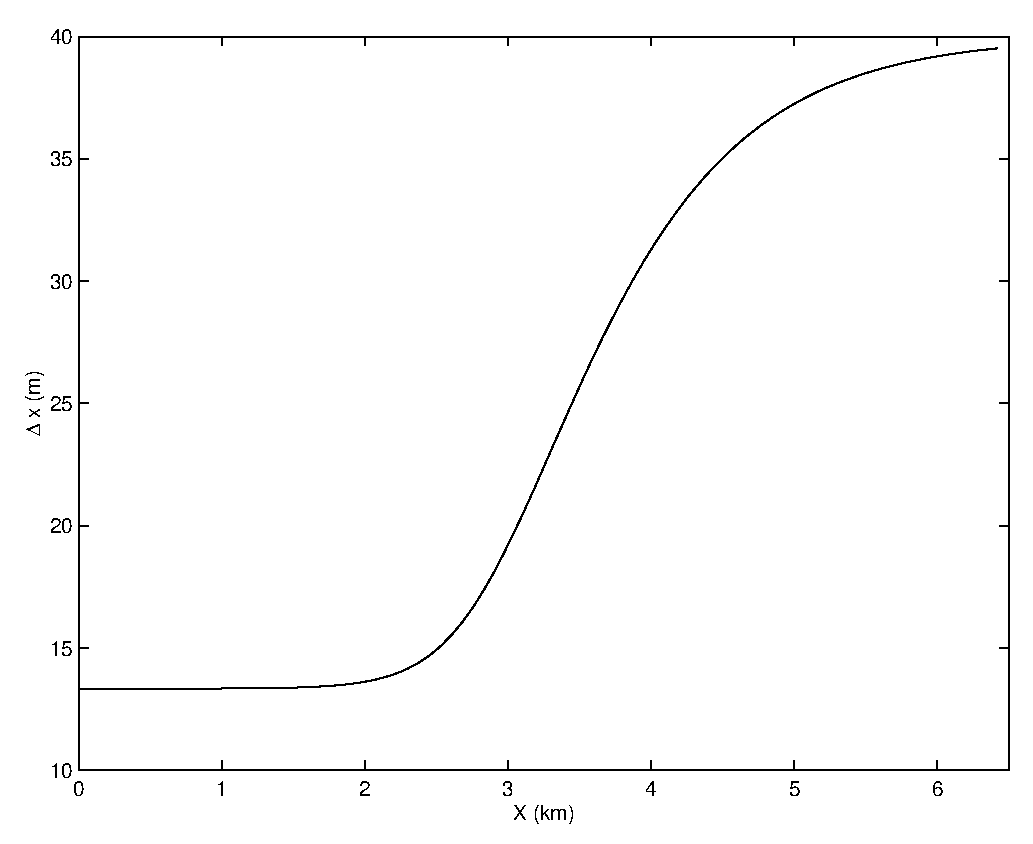
\includegraphics[width=\textwidth,height=.3\textheight]{s_examples/plume_on_slope/dx.eps}
\end{center}
\caption{Horizontal grid spacing, $\Delta x$, in the across-slope
direction for the gravity plume experiment.}
\label{fig:dx-plume-on-slope}
\end{figure}

\begin{figure}
\begin{center}
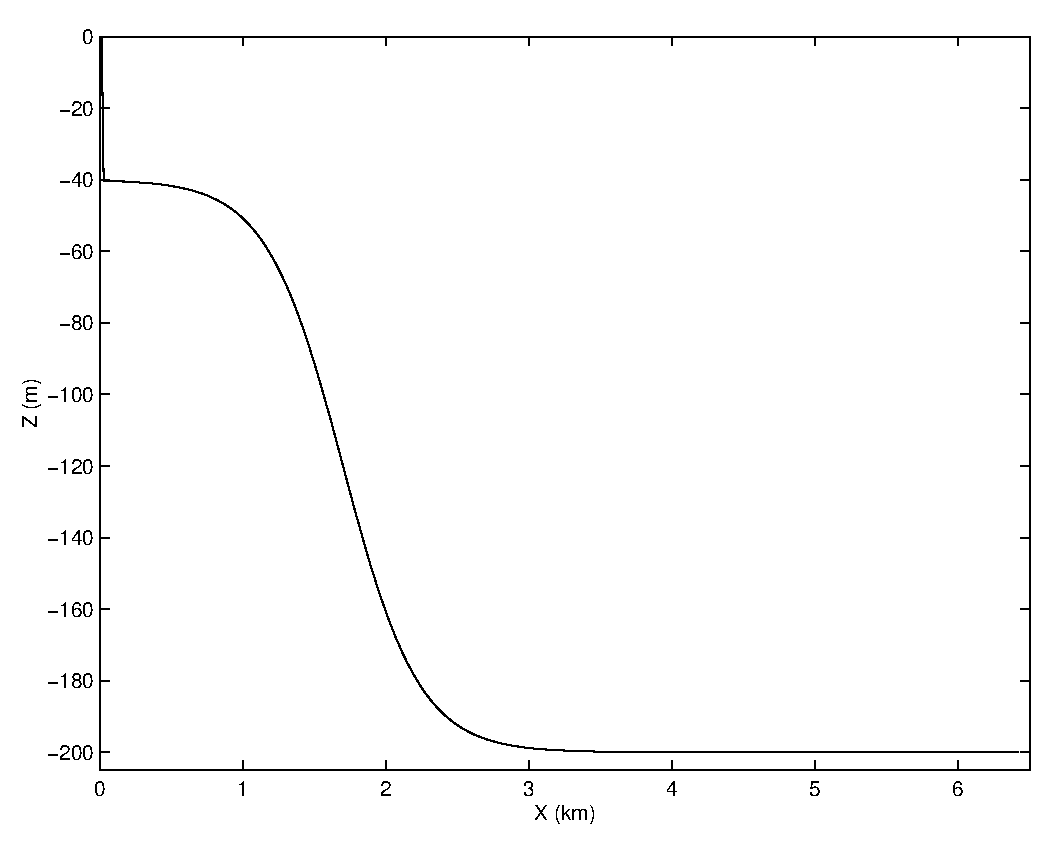
\includegraphics[width=\textwidth,height=.3\textheight]{s_examples/plume_on_slope/Depth.eps}
\end{center}
\caption{Topography, $h(x)$, used for the gravity plume experiment.}
\label{fig:depth-plume-on-slope}
\end{figure}

\begin{figure}
\begin{center}
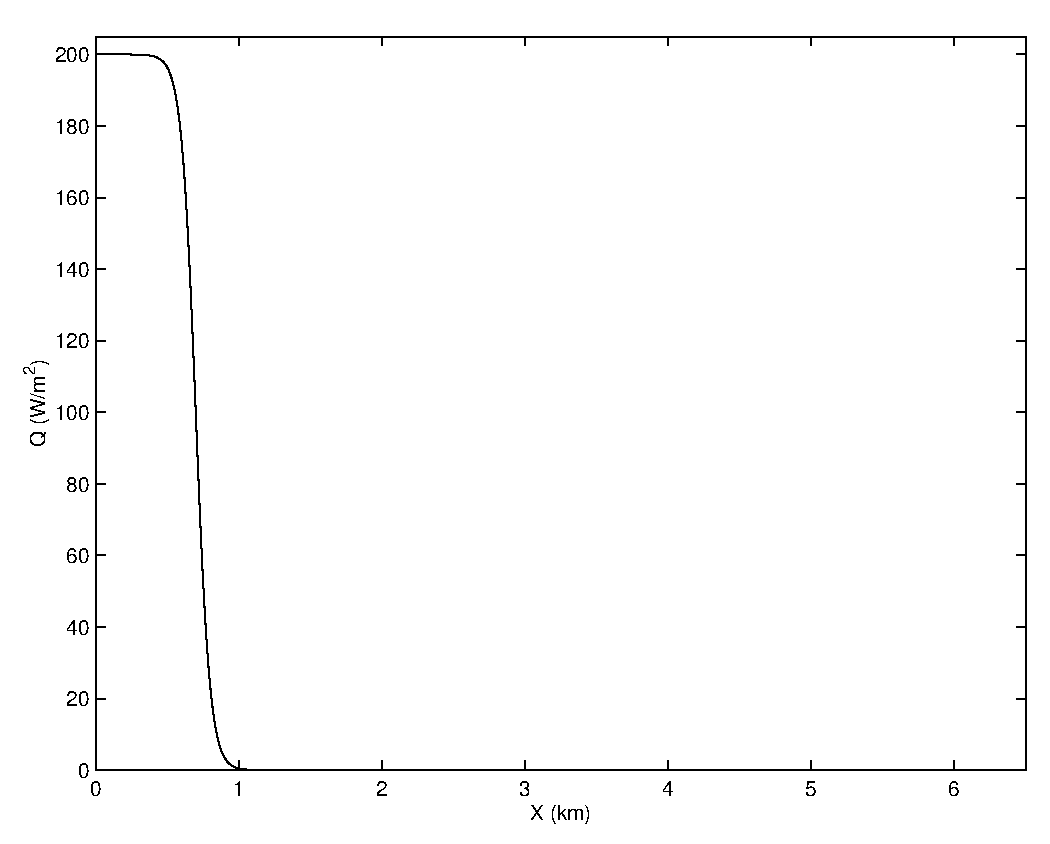
\includegraphics[width=\textwidth,height=.3\textheight]{s_examples/plume_on_slope/Qsurf.eps}
\end{center}
\caption{Upward surface heat flux, $Q(x)$, used as forcing in the
gravity plume experiment.}
\label{fig:Q-plume-on-slope}
\end{figure}

The domain is $200$~m deep and $6.4$~km across. Uniform resolution of
$60\times3^1/_3$~m is used in the vertical and variable resolution of
the form shown in Fig.~\ref{fig:dx-plume-on-slope} with $320$ points
is usedin the horizontal. The formula for $\Delta x$ is:
\begin{displaymath}
\Delta x(i) = \Delta x_1 + ( \Delta x_2 - \Delta x_1 )
( 1 + \tanh{\left(\frac{i-i_s}{w}\right)} ) /2
\end{displaymath}
where
\begin{eqnarray*}
Nx & = & 320 \\
Lx & = & 6400 \;\; \mbox{(m)} \\
\Delta x_1 & = & \frac{2}{3} \frac{Lx}{Nx} \;\; \mbox{(m)} \\
\Delta x_2 & = & \frac{Lx/2}{Nx-Lx/2 \Delta x_1} \;\; \mbox{(m)} \\
i_s & = & Lx/( 2 \Delta x_1 ) \\
w & = & 40 
\end{eqnarray*}
Here, $\Delta x_1$ is the resolution on the shelf, $\Delta x_2$ is the
resolution in deep water and $Nx$ is the number of points in the
horizontal.

The topography, shown in Fig.~\ref{fig:depth-plume-on-slope}, is given
by:
\begin{displaymath}
H(x) = -H_o + (H_o - h_s) ( 1 + \tanh{\left(\frac{x-x_s}{L_s}\right)} ) / 2
\end{displaymath}
where
\begin{eqnarray*}
H_o & = & 200 \;\; \mbox{(m)} \\
h_s & = & 40 \;\; \mbox{(m)} \\
x_s & = & 1500 + Lx/2 \;\; \mbox{(m)} \\
L_s & = & \frac{(H_o - h_s)}{2 s} \;\; \mbox{(m)} \\
s & = & 0.15
\end{eqnarray*}
Here, $s$ is the maximum slope, $H_o$ is the maximum depth, $h_s$ is
the shelf depth, $x_s$ is the lateral position of the shelf-break and
$L_s$ is the length-scale of the slope.

The forcing is through heat loss over the shelf, shown in
Fig.~\ref{fig:Q-plume-on-slope} and takes the form of a fixed flux
with profile:
\begin{displaymath}
Q(x) = Q_o ( 1 + \tanh{\left(\frac{x - x_q}{L_q}\right)} ) / 2
\end{displaymath}
where
\begin{eqnarray*}
Q_o & = & 200 \;\; \mbox{(W m$^{-2}$)} \\
x_q & = & 2500 + Lx/2 \;\; \mbox{(m)} \\
L_q & = & 100 \;\; \mbox{(m)}
\end{eqnarray*}
Here, $Q_o$, is the maximum heat flux, $x_q$ is the position of the
cut-off and $L_q$ is the width of the cut-off.

The initial tempeture field is unstratified but with random
perturbations, to induce convection early on in the run. The random
perturbation are calculated in computational space and because of the
variable resolution introduce some spatial correlations but this does
not matter for this experiment. The perturbations have range
$0-0.01$~$^{\circ}\mathrm{K}$.

\subsection{Code configuration}
\label{www:tutorials}
\label{sect:plume-config}

The computational domain (number of points) is specified in {\tt
code/SIZE.h} and is configured as a single tile of dimensions
$320\times1\times60$. There are no experiment specific source files.

Optional code required to for this experiment are the non-hydrostatic
algorithm and open-boundaries:
\begin{itemize}
\item Non-hydrostatic terms and algorithm are enabled with {\bf
\#define ALLOW\_NONHYDROSTATIC} in {\tt code/CPP\_OPTIONS.h} and
activated with {\bf nonHydrostatic=.TRUE.,} in namelist {\em PARM01}
of {\tt input/data}.
\item Open boundaries are enabled by adding line {\bf obcs} to 
package configuration file
{\tt code/packages.conf} and activated via {\bf useOBCS=.TRUE,} in
namelist {\em PACKAGES} of {\tt input/data.pkg}.
\end{itemize}

\subsection{Model parameters}
\label{www:tutorials}
\label{sect:plume-params}

\begin{table}
\begin{center}
\begin{tabular}{lll}
$g$ & $9.81$ m s$^{-2}$ & acceleration due to gravity \\
$\rho_o$ & $999.8$ kg m$^{-3}$ & reference density \\
$\alpha$ & $2 \times 10^{-4}$ K$^{-1}$ & expansion coefficient \\
$A_h$ & $1 \times 10^{-2}$ m$^2$s$^{-1}$ & horizontal viscosity \\
$A_v$ & $1 \times 10^{-3}$ m$^2$s$^{-1}$ & vertical viscosity \\
$\kappa_h$ & $0$ m$^2$s$^{-1}$ & (explicit) horizontal diffusion \\
$\kappa_v$ & $0$ m$^2$s$^{-1}$ & (explicit) vertical diffusion \\
\\
$\Delta t$ & $20$ s & time step \\
$\Delta z$ & $3.3\dot{3}$ m & vertical grid spacing \\
$\Delta x$ & $13.\dot{3}-39.5$ m & horizontal grid spacing
\end{tabular}
\end{center}
\caption{Model parameters used in the gravity plume experiment.}
\label{table:plume-on-slope}
\end{table}

The model parameters (Table~\ref{table:plume-on-slope}) are specified
in {\tt input/data} and if not assume the default values defined in
{\tt model/src/set\_defaults.F}. A linear equation of state is used,
{\bf eosType='LINEAR'}, but only temperature is active, {\bf
sBeta=0.E-4}. For the given heat flux, $Q_o$, the buoyancy forcing is
$B_o = \frac{g \alpha Q}{\rho_o c_p} \sim
10^{-7}$~m$^2$s$^{-3}$. Using $R=10^3$~m, the shelf width, then this
gives a velocity scale of $U\sim 5 \times 10^{-2}$~m~s$^-1$ for the
initial front but will accelerate by an order of magnitude over the
slope. The temperature anomaly will be of order $\Delta \theta \sim 3
\times 10^{-2}$~K.  The viscosity is constant and gives a Reynolds
number of $100$, using $h=20$~m for the initial front and will be an
order magnitude bigger over the slope. There is no explicit diffusion
but a non-linear advection scheme is used for temperature which adds
enough diffusion so as to keep the model stable. The time-step is set
to $20$~s and gives Courant number order one when the flow reaches the
bottom of the slope.

\subsection{Build and run the model}
\label{www:tutorials}

Build the model per usual. For example:
\begin{verbatim}
% cd verification/plume_on_slope
% mkdir build
% cd build
% ../../../tools/genmake -mods=../code -disable=gmredi,kpp,zonal_filt
  ,shap_filt
% make depend
% make
\end{verbatim}

When compilation is complete, run the model as usual, for example:
\begin{verbatim}
% cd ../
% mkdir run
% cp input/* build/mitgcmuv run/
% cd run
% ./mitgcmuv > output.txt
\end{verbatim}


%\pagebreak

% Section: Software Architecture
% $Header: /u/gcmpack/manual/s_software/text/top_section.tex,v 1.1.1.1 2001/08/08 16:16:19 adcroft Exp $
% $Name:  $

\chapter{Software Architecture}

%\pagebreak


%\part{Adjoint of the MIT GCM}

% Section: Automatic Differentiation
% $Header: /u/gcmpack/manual/s_autodiff/text/top_section.tex,v 1.10 2010/08/27 13:09:40 jmc Exp $
% $Name:  $

\chapter{Automatic Differentiation}
\begin{rawhtml}
<!-- CMIREDIR:automatic_differentiation: -->
\end{rawhtml}



% $Header: /u/gcmpack/manual/s_autodiff/text/doc_ad_2.tex,v 1.15 2002/04/24 11:01:46 heimbach Exp $
% $Name:  $

{\sf Automatic differentiation} (AD), also referred to as algorithmic
(or, more loosely, computational) differentiation, involves 
automatically deriving code to calculate
partial derivatives from an existing fully non-linear prognostic code.
(see \cite{gri:00}).
A software tool is used that parses and transforms source files 
according to a set of linguistic and mathematical rules. 
AD tools are like source-to-source translators in that
they parse a program code as input and produce a new program code 
as output.
However, unlike a pure source-to-source translation, the output program
represents a new algorithm, such as the evaluation of the
Jacobian, the Hessian, or higher derivative operators.
In principle, a variety of derived algorithms
can be generated automatically in this way.

The MITGCM has been adapted for use with the
Tangent linear and Adjoint Model Compiler (TAMC) and its successor TAF
(Transformation of Algorithms in Fortran), developed
by Ralf Giering (\cite{gie-kam:98}, \cite{gie:99,gie:00}).
The first application of the adjoint of the MITGCM for sensitivity
studies has been published by \cite{maro-eta:99}.
\cite{sta-eta:97,sta-eta:01} use the MITGCM and its adjoint
for ocean state estimation studies.
In the following we shall refer to TAMC and TAF synonymously,
except were explicitly stated otherwise.

TAMC exploits the chain rule for computing the first
derivative of a function with
respect to a set of input variables. 
Treating a given forward code as a composition of operations --
each line representing a compositional element, the chain rule is
rigorously applied to the code, line by line. The resulting 
tangent linear or adjoint code,
then, may be thought of as the composition in 
forward or reverse order, respectively, of the
Jacobian matrices of the forward code's compositional elements.

%**********************************************************************
\section{Some basic algebra}
\label{sec_ad_algebra}
%**********************************************************************

Let $ \cal{M} $ be a general nonlinear, model, i.e. a
mapping from the $m$-dimensional space 
$U \subset I\!\!R^m$ of input variables 
$\vec{u}=(u_1,\ldots,u_m)$
(model parameters, initial conditions, boundary conditions
such as forcing functions) to the $n$-dimensional space 
$V \subset I\!\!R^n$ of 
model output variable $\vec{v}=(v_1,\ldots,v_n)$ 
(model state, model diagnostics, objective function, ...) 
under consideration,
%
\begin{equation}
\begin{split}
{\cal M} \, : & \, U \,\, \longrightarrow \, V \\
~      & \, \vec{u} \,\, \longmapsto \, \vec{v} \, = \, 
{\cal M}(\vec{u}) 
\label{fulloperator}
\end{split}
\end{equation}
%
The vectors $ \vec{u} \in U $ and $ v \in V $ may be represented w.r.t.
some given basis vectors
$ {\rm span} (U) = \{ {\vec{e}_i} \}_{i = 1, \ldots , m} $ and
$ {\rm span} (V) = \{ {\vec{f}_j} \}_{j = 1, \ldots , n} $ as
\[
\vec{u} \, = \, \sum_{i=1}^{m} u_i \, {\vec{e}_i},
\qquad
\vec{v} \, = \, \sum_{j=1}^{n} v_j \, {\vec{f}_j}
\]

Two routes may be followed to determine the sensitivity of the 
output variable $\vec{v}$ to its input $\vec{u}$.

\subsection{Forward or direct sensitivity}
%
Consider a perturbation to the input variables $\delta \vec{u}$
(typically a single component 
$\delta \vec{u} = \delta u_{i} \, {\vec{e}_{i}}$).
Their effect on the output may be obtained via the linear
approximation of the model $ {\cal M}$ in terms of its Jacobian matrix
$ M $, evaluated in the point $u^{(0)}$ according to
%
\begin{equation}
\delta \vec{v} \, = \, M |_{\vec{u}^{(0)}} \, \delta \vec{u}
\label{tangent_linear}
\end{equation}
with resulting output perturbation $\delta \vec{v}$.
In components
$M_{j i} \, = \, \partial {\cal M}_{j} / \partial u_{i} $, 
it reads
%
\begin{equation}
\delta v_{j} \, = \, \sum_{i} 
\left. \frac{\partial {\cal M}_{j}}{\partial u_{i}} \right|_{u^{(0)}} \, 
\delta u_{i}
\label{jacobi_matrix}
\end{equation}
%
Eq. (\ref{tangent_linear}) is the {\sf tangent linear model (TLM)}.
In contrast to the full nonlinear model $ {\cal M} $, the operator
$ M $ is just a matrix
which can readily be used to find the forward sensitivity of $\vec{v}$ to 
perturbations in  $u$,
but if there are very many input variables $(\gg O(10^{6})$ for 
large-scale oceanographic application), it quickly becomes 
prohibitive to proceed directly as in (\ref{tangent_linear}),
if the impact of each component $ {\bf e_{i}} $ is to be assessed. 

\subsection{Reverse or adjoint sensitivity}
%
Let us consider the special case of a
scalar objective function ${\cal J}(\vec{v})$ of the model output (e.g. 
the total meridional heat transport, 
the total uptake of $CO_{2}$ in the Southern 
Ocean over a time interval,
or a measure of some model-to-data misfit)
%
\begin{eqnarray}
\begin{array}{cccccc}
{\cal J}  \, : &  U & 
\longrightarrow & V &   
\longrightarrow & I \!\! R \\
~       &  \vec{u} & \longmapsto     & \vec{v}={\cal M}(\vec{u}) & 
\longmapsto     & {\cal J}(\vec{u}) = {\cal J}({\cal M}(\vec{u}))
\end{array}
\label{compo}
\end{eqnarray}
%
The perturbation of $ {\cal J} $ around a fixed point $ {\cal J}_0 $,
\[
{\cal J} \, = \, {\cal J}_0 \, + \, \delta {\cal J}
\]
can be expressed in both bases of $ \vec{u} $ and $ \vec{v} $
w.r.t. their corresponding inner product 
$\left\langle \,\, , \,\, \right\rangle $ 
%
\begin{equation}
\begin{split}
{\cal J} & = \,
{\cal J} |_{\vec{u}^{(0)}} \, + \, 
\left\langle \, \nabla _{u}{\cal J}^T |_{\vec{u}^{(0)}} \, , \, \delta \vec{u} \, \right\rangle 
\, + \, O(\delta \vec{u}^2) \\
~ & = \,
{\cal J} |_{\vec{v}^{(0)}} \, + \, 
\left\langle \, \nabla _{v}{\cal J}^T |_{\vec{v}^{(0)}} \, , \, \delta \vec{v} \, \right\rangle
\, + \, O(\delta \vec{v}^2)
\end{split}
\label{deljidentity}
\end{equation}
%
(note, that the gradient $ \nabla f $ is a co-vector, therefore
its transpose is required in the above inner product).
Then, using the representation of 
$ \delta {\cal J} = 
\left\langle \, \nabla _{v}{\cal J}^T \, , \, \delta \vec{v} \, \right\rangle $,
the definition 
of an adjoint operator $ A^{\ast} $ of a given operator $ A $,
\[ 
\left\langle \, A^{\ast} \vec{x} \, , \, \vec{y} \, \right\rangle =
\left\langle \, \vec{x} \, , \,  A \vec{y} \, \right\rangle 
\]
which for finite-dimensional vector spaces is just the 
transpose of $ A $,
\[
A^{\ast} \, = \, A^T
\]
and from eq. (\ref{tangent_linear}), (\ref{deljidentity}),
we note that
(omitting $|$'s):
%
\begin{equation}
\delta {\cal J}
\, = \,
\left\langle \, \nabla _{v}{\cal J}^T \, , \, \delta \vec{v} \, \right\rangle
\, = \,
\left\langle \, \nabla _{v}{\cal J}^T \, , \, M \, \delta \vec{u} \, \right\rangle
\, = \, 
\left\langle \, M^T \, \nabla _{v}{\cal J}^T \, , \, 
\delta \vec{u} \, \right\rangle
\label{inner}
\end{equation}
%
With the identity (\ref{deljidentity}), we then find that
the gradient $ \nabla _{u}{\cal J} $ can be readily inferred by 
invoking the adjoint $ M^{\ast } $ of the tangent linear model $ M $
%
\begin{equation}
\begin{split}
\nabla _{u}{\cal J}^T |_{\vec{u}} & 
= \, M^T |_{\vec{u}} \cdot \nabla _{v}{\cal J}^T |_{\vec{v}}  \\
~ & = \, M^T |_{\vec{u}} \cdot \delta \vec{v}^{\ast} \\
~ & = \, \delta \vec{u}^{\ast}
\end{split}
\label{adjoint}
\end{equation}
%
Eq. (\ref{adjoint}) is the {\sf adjoint model (ADM)}, 
in which $M^T$ is the adjoint (here, the transpose) of the 
tangent linear operator $M$, $ \delta \vec{v}^{\ast} $ 
the adjoint variable of the model state $ \vec{v} $, and
$ \delta \vec{u}^{\ast} $ the adjoint variable of the control variable $ \vec{u} $.

The {\sf reverse} nature of the adjoint calculation can be readily 
seen as follows. 
Consider a model integration which consists of $ \Lambda $
consecutive operations
$ {\cal M}_{\Lambda} (  {\cal M}_{\Lambda-1} ( 
...... ( {\cal M}_{\lambda} (
......
( {\cal M}_{1} ( {\cal M}_{0}(\vec{u}) )))) $,
where the ${\cal M}$'s could be the elementary steps, i.e. single lines
in the code of the model, or successive time steps of the
model integration, 
starting at step 0 and moving up to step $\Lambda$, with intermediate
${\cal M}_{\lambda} (\vec{u}) = \vec{v}^{(\lambda+1)}$ and final 
${\cal M}_{\Lambda} (\vec{u}) = \vec{v}^{(\Lambda+1)} = \vec{v}$.
Let ${\cal J}$ be a cost function which explicitly depends on the
final state $\vec{v}$ only
(this restriction is for clarity reasons only).
%
${\cal J}(u)$ may be decomposed according to:
%
\begin{equation}
{\cal J}({\cal M}(\vec{u})) \, = \, 
{\cal J} ( {\cal M}_{\Lambda} (  {\cal M}_{\Lambda-1} ( 
...... ( {\cal M}_{\lambda} (
......
( {\cal M}_{1} ( {\cal M}_{0}(\vec{u}) )))))
\label{compos}
\end{equation}
%
Then, according to the chain rule, the forward calculation reads, 
in terms of the Jacobi matrices
(we've omitted the $ | $'s which, nevertheless are important
to the aspect of {\it tangent} linearity;
note also that by definition
$ \langle \, \nabla _{v}{\cal J}^T \, , \, \delta \vec{v} \, \rangle
= \nabla_v {\cal J} \cdot \delta \vec{v} $ )
%
\begin{equation}
\begin{split}
\nabla_v {\cal J} (M(\delta \vec{u})) & = \,
\nabla_v {\cal J} \cdot M_{\Lambda}
\cdot ...... \cdot M_{\lambda} \cdot ...... \cdot
M_{1} \cdot M_{0} \cdot \delta \vec{u} \\
~ & = \, \nabla_v {\cal J} \cdot \delta \vec{v} \\
\end{split}
\label{forward}
\end{equation}
%
whereas in reverse mode we have
%
\begin{equation}
\boxed{
\begin{split}
M^T ( \nabla_v {\cal J}^T) & = \,
M_{0}^T \cdot M_{1}^T
\cdot ...... \cdot M_{\lambda}^T \cdot ...... \cdot 
M_{\Lambda}^T \cdot \nabla_v {\cal J}^T \\
~ & = \, M_{0}^T \cdot M_{1}^T
\cdot ...... \cdot 
\nabla_{v^{(\lambda)}} {\cal J}^T \\
~ & = \, \nabla_u {\cal J}^T
\end{split}
}
\label{reverse}
\end{equation}
%
clearly expressing the reverse nature of the calculation.
Eq. (\ref{reverse}) is at the heart of automatic adjoint compilers.
If the intermediate steps $\lambda$ in 
eqn. (\ref{compos}) -- (\ref{reverse})
represent the model state (forward or adjoint) at each 
intermediate time step as noted above, then correspondingly,
$ M^T (\delta \vec{v}^{(\lambda) \, \ast}) = 
\delta \vec{v}^{(\lambda-1) \, \ast} $ for the adjoint variables.
It thus becomes evident that the adjoint calculation also
yields the adjoint of each model state component 
$ \vec{v}^{(\lambda)} $ at each intermediate step $ \lambda $, namely
%
\begin{equation}
\boxed{
\begin{split}
\nabla_{v^{(\lambda)}} {\cal J}^T |_{\vec{v}^{(\lambda)}}
& = \,
M_{\lambda}^T |_{\vec{v}^{(\lambda)}} \cdot ...... \cdot 
M_{\Lambda}^T |_{\vec{v}^{(\lambda)}} \cdot \delta \vec{v}^{\ast} \\
~ & = \, \delta \vec{v}^{(\lambda) \, \ast}
\end{split}
}
\end{equation}
%
in close analogy to eq. (\ref{adjoint})
We note in passing that that the $\delta \vec{v}^{(\lambda) \, \ast}$
are the Lagrange multipliers of the model equations which determine
$ \vec{v}^{(\lambda)}$.

In components, eq. (\ref{adjoint}) reads as follows.
Let
\[
\begin{array}{rclcrcl}
\delta \vec{u} & = &
\left( \delta u_1,\ldots, \delta u_m \right)^T , & \qquad &
\delta \vec{u}^{\ast} \,\, = \,\, \nabla_u {\cal J}^T & = &
\left( 
\frac{\partial {\cal J}}{\partial u_1},\ldots, 
\frac{\partial {\cal J}}{\partial u_m}
\right)^T \\
\delta \vec{v} & = &
\left( \delta v_1,\ldots, \delta u_n \right)^T , & \qquad &
\delta \vec{v}^{\ast} \,\, = \,\, \nabla_v {\cal J}^T & = &
\left( 
\frac{\partial {\cal J}}{\partial v_1},\ldots, 
\frac{\partial {\cal J}}{\partial v_n}
\right)^T \\
\end{array}
\]
denote the perturbations in $\vec{u}$ and $\vec{v}$, respectively,
and their adjoint variables;
further
\[
M \, = \, \left(
\begin{array}{ccc}
\frac{\partial {\cal M}_1}{\partial u_1} & \ldots &
\frac{\partial {\cal M}_1}{\partial u_m} \\
\vdots & ~ & \vdots \\
\frac{\partial {\cal M}_n}{\partial u_1} & \ldots &
\frac{\partial {\cal M}_n}{\partial u_m} \\
\end{array}
\right)
\]
is the Jacobi matrix of $ {\cal M} $ 
(an $ n \times m $ matrix)
such that $ \delta \vec{v} = M \cdot \delta \vec{u} $, or
\[
\delta v_{j} 
\, = \, \sum_{i=1}^m M_{ji} \, \delta u_{i}
\, = \, \sum_{i=1}^m \, \frac{\partial {\cal M}_{j}}{\partial u_{i}} 
\delta u_{i}
\]
%
Then eq. (\ref{adjoint}) takes the form
\[
\delta u_{i}^{\ast} 
\, = \, \sum_{j=1}^n M_{ji} \, \delta v_{j}^{\ast}
\, = \, \sum_{j=1}^n \, \frac{\partial {\cal M}_{j}}{\partial u_{i}} 
\delta v_{j}^{\ast}
\]
%
or
%
\[
\left(
\begin{array}{c}
\left. \frac{\partial}{\partial u_1} {\cal J} \right|_{\vec{u}^{(0)}} \\
\vdots \\
\left. \frac{\partial}{\partial u_m} {\cal J} \right|_{\vec{u}^{(0)}} \\
\end{array}
\right)
\, = \,
\left(
\begin{array}{ccc}
\left. \frac{\partial {\cal M}_1}{\partial u_1} \right|_{\vec{u}^{(0)}} 
& \ldots &
\left. \frac{\partial {\cal M}_n}{\partial u_1} \right|_{\vec{u}^{(0)}} \\
\vdots & ~ & \vdots \\
\left. \frac{\partial {\cal M}_1}{\partial u_m} \right|_{\vec{u}^{(0)}} 
& \ldots &
\left. \frac{\partial {\cal M}_n}{\partial u_m} \right|_{\vec{u}^{(0)}} \\
\end{array}
\right)
\cdot
\left(
\begin{array}{c}
\left. \frac{\partial}{\partial v_1} {\cal J} \right|_{\vec{v}} \\
\vdots \\
\left. \frac{\partial}{\partial v_n} {\cal J} \right|_{\vec{v}} \\
\end{array}
\right)
\]
%
Furthermore, the adjoint  $ \delta v^{(\lambda) \, \ast} $
of any intermediate state $ v^{(\lambda)} $
may be obtained, using the intermediate Jacobian
(an $ n_{\lambda+1} \times n_{\lambda} $ matrix)
%
\[
M_{\lambda} \, = \,
\left(
\begin{array}{ccc}
\frac{\partial ({\cal M}_{\lambda})_1}{\partial v^{(\lambda)}_1}
& \ldots &
\frac{\partial ({\cal M}_{\lambda})_1}{\partial v^{(\lambda)}_{n_{\lambda}}} \\
\vdots & ~ & \vdots \\
\frac{\partial ({\cal M}_{\lambda})_{n_{\lambda+1}}}{\partial v^{(\lambda)}_1}
& \ldots &
\frac{\partial ({\cal M}_{\lambda})_{n_{\lambda+1}}}{\partial v^{(\lambda)}_{n_{\lambda}}} \\
\end{array}
\right)
\]
%
and the shorthand notation for the adjoint variables
$ \delta v^{(\lambda) \, \ast}_{j} = \frac{\partial}{\partial v^{(\lambda)}_{j}} 
{\cal J}^T $, $ j = 1, \ldots , n_{\lambda} $, 
for intermediate components, yielding
\begin{equation}
\small
\begin{split}
\left(
\begin{array}{c}
\delta v^{(\lambda) \, \ast}_1 \\
\vdots \\
\delta v^{(\lambda) \, \ast}_{n_{\lambda}} \\
\end{array}
\right)
\, = &
\left(
\begin{array}{ccc}
\frac{\partial ({\cal M}_{\lambda})_1}{\partial v^{(\lambda)}_1}
& \ldots \,\, \ldots &
\frac{\partial ({\cal M}_{\lambda})_{n_{\lambda+1}}}{\partial v^{(\lambda)}_1} \\
\vdots & ~ & \vdots \\
\frac{\partial ({\cal M}_{\lambda})_1}{\partial v^{(\lambda)}_{n_{\lambda}}}
& \ldots \,\, \ldots  &
\frac{\partial ({\cal M}_{\lambda})_{n_{\lambda+1}}}{\partial v^{(\lambda)}_{n_{\lambda}}} \\
\end{array}
\right)
\cdot
%
\\ ~ & ~
\\ ~ &
%
\left(
\begin{array}{ccc}
\frac{\partial ({\cal M}_{\lambda+1})_1}{\partial v^{(\lambda+1)}_1}
& \ldots &
\frac{\partial ({\cal M}_{\lambda+1})_{n_{\lambda+2}}}{\partial v^{(\lambda+1)}_1} \\
\vdots & ~ & \vdots \\
\vdots & ~ & \vdots \\
\frac{\partial ({\cal M}_{\lambda+1})_1}{\partial v^{(\lambda+1)}_{n_{\lambda+1}}}
& \ldots  &
\frac{\partial ({\cal M}_{\lambda+1})_{n_{\lambda+2}}}{\partial v^{(\lambda+1)}_{n_{\lambda+1}}} \\
\end{array}
\right)
\cdot \, \ldots \, \cdot
\left(
\begin{array}{c}
\delta v^{\ast}_1 \\
\vdots \\
\delta v^{\ast}_{n} \\
\end{array}
\right)
\end{split}
\end{equation}

Eq. (\ref{forward}) and (\ref{reverse}) are perhaps clearest in
showing the advantage of the reverse over the forward mode
if the gradient $\nabla _{u}{\cal J}$, i.e. the sensitivity of the
cost function $ {\cal J} $ with respect to {\it all} input
variables $u$
(or the sensitivity of the cost function with respect to
{\it all} intermediate states $ \vec{v}^{(\lambda)} $) are sought.
In order to be able to solve for each component of the gradient
$ \partial {\cal J} / \partial u_{i} $ in (\ref{forward})
a forward calculation has to be performed for each component separately,
i.e. $ \delta \vec{u} = \delta u_{i} {\vec{e}_{i}} $ 
for  the $i$-th forward calculation. 
Then, (\ref{forward}) represents the
projection of $ \nabla_u {\cal J} $ onto the $i$-th component.
The full gradient is retrieved from the $ m $ forward calculations.
In contrast, eq. (\ref{reverse}) yields the full 
gradient $\nabla _{u}{\cal J}$ (and all intermediate gradients
$\nabla _{v^{(\lambda)}}{\cal J}$) within a single reverse calculation.

Note, that if $ {\cal J} $ is a vector-valued function
of dimension $ l > 1 $,
eq. (\ref{reverse}) has to be modified according to
\[
M^T \left( \nabla_v {\cal J}^T \left(\delta \vec{J}\right) \right) 
\, = \,
\nabla_u {\cal J}^T \cdot \delta \vec{J}
\]
where now $ \delta \vec{J} \in I\!\!R^l $ is a vector of 
dimension $ l $.
In this case $ l $ reverse simulations have to be performed
for each $ \delta J_{k}, \,\, k = 1, \ldots, l $.
Then, the reverse mode is more efficient as long as
$ l < n $, otherwise the forward mode is preferable.
Strictly, the reverse mode is called adjoint mode only for
$ l = 1 $.

A detailed analysis of the underlying numerical operations 
shows that the computation of $\nabla _{u}{\cal J}$ in this way
requires about 2 to 5 times the computation of the cost function.
Alternatively, the gradient vector could be approximated
by finite differences, requiring $m$ computations
of the perturbed cost function.

To conclude we give two examples of commonly used types
of cost functions:

\paragraph{Example 1: 
$ {\cal J} = v_{j} (T) $} ~ \\
The cost function consists of the $j$-th component of the model state
$ \vec{v} $ at time $T$. 
Then $ \nabla_v {\cal J}^T = {\vec{f}_{j}} $ is just the $j$-th
unit vector. The $ \nabla_u {\cal J}^T $ 
is the projection of the adjoint
operator onto the $j$-th component ${\bf f_{j}}$,
\[
\nabla_u {\cal J}^T 
\, = \, M^T \cdot \nabla_v {\cal J}^T
\, = \,  \sum_{i} M^T_{ji} \, {\vec{e}_{i}}
\]

\paragraph{Example 2: 
$ {\cal J} = \langle \, {\cal H}(\vec{v}) - \vec{d} \, , 
 \, {\cal H}(\vec{v}) - \vec{d} \, \rangle $} ~ \\
The cost function represents the quadratic model vs. data misfit.
Here, $ \vec{d} $ is the data vector and $ {\cal H} $ represents the
operator which maps the model state space onto the data space.
Then, $ \nabla_v {\cal J} $ takes the form
%
\begin{equation*}
\begin{split}
\nabla_v {\cal J}^T & = \, 2 \, \, H \cdot 
\left( \, {\cal H}(\vec{v}) - \vec{d} \, \right) \\
~          & = \, 2 \sum_{j} \left\{ \sum_k
\frac{\partial {\cal H}_k}{\partial v_{j}} 
\left( {\cal H}_k (\vec{v}) - d_k \right)
\right\} \, {\vec{f}_{j}} \\
\end{split}
\end{equation*}
%
where $H_{kj} = \partial {\cal H}_k / \partial v_{j} $ is the 
Jacobi matrix of the data projection operator.
Thus, the gradient $ \nabla_u {\cal J} $ is given by the 
adjoint operator,
driven by the model vs. data misfit:
\[
\nabla_u {\cal J}^T \, = \, 2 \, M^T \cdot 
H \cdot \left( {\cal H}(\vec{v}) - \vec{d} \, \right)
\]

\subsection{Storing vs. recomputation in reverse mode}
\label{checkpointing}

We note an important aspect of the forward vs. reverse 
mode calculation.
Because of the local character of the derivative
(a derivative is defined w.r.t. a point along the trajectory),
the intermediate results of the model trajectory
$\vec{v}^{(\lambda+1)}={\cal M}_{\lambda}(v^{(\lambda)})$ 
may be required to evaluate the intermediate Jacobian 
$M_{\lambda}|_{\vec{v}^{(\lambda)}} \, \delta \vec{v}^{(\lambda)} $.
This is the case e.g. for nonlinear expressions
(momentum advection, nonlinear equation of state), state-dependent
conditional statements (parameterization schemes).
In the forward mode, the intermediate results are required
in the same order as computed by the full forward model ${\cal M}$,
but in the reverse mode they are required in the reverse order.
Thus, in the reverse mode the trajectory of the forward model
integration ${\cal M}$ has to be stored to be available in the reverse
calculation. Alternatively, the complete model state up to the
point of evaluation has to be recomputed whenever its value is required.

A method to balance the amount of recomputations vs.
storage requirements is called {\sf checkpointing}
(e.g. \cite{gri:92}, \cite{res-eta:98}).
It is depicted in \ref{fig:3levelcheck} for a 3-level checkpointing
[as an example, we give explicit numbers for a 3-day 
integration with a 1-hourly timestep in square brackets].
\begin{itemize}
%
\item [$lev3$]
In a first step, the model trajectory is subdivided into 
$ {n}^{lev3} $ subsections [$ {n}^{lev3} $=3 1-day intervals],
with the label $lev3$ for this outermost loop.
The model is then integrated along the full trajectory,
and the model state stored to disk only at every $ k_{i}^{lev3} $-th timestep 
[i.e. 3 times, at
$ i = 0,1,2 $ corresponding to $ k_{i}^{lev3} = 0, 24, 48 $].
In addition, the cost function is computed, if needed.
%
\item [$lev2$]
In a second step each subsection itself is divided into
$ {n}^{lev2} $ subsections
[$ {n}^{lev2} $=4 6-hour intervals per subsection].
The model picks up at the last outermost dumped state 
$ v_{k_{n}^{lev3}} $ and is integrated forward in time along
the last subsection, with the label $lev2$ for this  
intermediate loop. 
The model state is now stored to disk at every $ k_{i}^{lev2} $-th 
timestep 
[i.e. 4 times, at
$ i = 0,1,2,3 $ corresponding to $ k_{i}^{lev2} = 48, 54, 60, 66 $].
%
\item [$lev1$]
Finally, the model picks up at the last intermediate dump state
$ v_{k_{n}^{lev2}} $ and is integrated forward in time along
the last subsection, with the label $lev1$ for this  
intermediate loop.
Within this sub-subsection only, parts of the model state is stored
to memory at every timestep 
[i.e. every hour $ i=0,...,5$ corresponding to 
$ k_{i}^{lev1} = 66, 67, \ldots, 71 $].
The  final state $ v_n = v_{k_{n}^{lev1}} $ is reached
and the model state of all preceding timesteps along the last
innermost subsection are available, enabling integration backwards
in time along the last subsection.
The adjoint can thus be computed along this last 
subsection $k_{n}^{lev2}$. 
%
\end{itemize}
%
This procedure is repeated consecutively for each previous
subsection $k_{n-1}^{lev2}, \ldots, k_{1}^{lev2} $
carrying the adjoint computation to the initial time 
of the subsection $k_{n}^{lev3}$.
Then, the procedure is repeated for the previous subsection
$k_{n-1}^{lev3}$ 
carrying the adjoint computation to the initial time 
$k_{1}^{lev3}$.

For the full model trajectory of
$ n^{lev3} \cdot n^{lev2} \cdot n^{lev1} $ timesteps
the required storing of the model state was significantly reduced to
$ n^{lev2} + n^{lev3} $ to disk and roughly $ n^{lev1} $ to memory
[i.e. for the 3-day integration with a total oof 72 timesteps
the model state was stored 7 times to disk and roughly 6 times
to memory].
This saving in memory comes at a cost of a required
3 full forward integrations of the model (one for each
checkpointing level).
The optimal balance of storage vs. recomputation certainly depends
on the computing resources available and may be adjusted by
adjusting the partitioning among the 
$ n^{lev3}, \,\, n^{lev2}, \,\, n^{lev1} $.

\begin{figure}[t!]
\begin{center}
%\psdraft
%\psfrag{v_k1^lev3}{\mathinfigure{v_{k_{1}^{lev3}}}}
%\psfrag{v_kn-1^lev3}{\mathinfigure{v_{k_{n-1}^{lev3}}}}
%\psfrag{v_kn^lev3}{\mathinfigure{v_{k_{n}^{lev3}}}}
%\psfrag{v_k1^lev2}{\mathinfigure{v_{k_{1}^{lev2}}}}
%\psfrag{v_kn-1^lev2}{\mathinfigure{v_{k_{n-1}^{lev2}}}}
%\psfrag{v_kn^lev2}{\mathinfigure{v_{k_{n}^{lev2}}}}
%\psfrag{v_k1^lev1}{\mathinfigure{v_{k_{1}^{lev1}}}}
%\psfrag{v_kn^lev1}{\mathinfigure{v_{k_{n}^{lev1}}}}
%\mbox{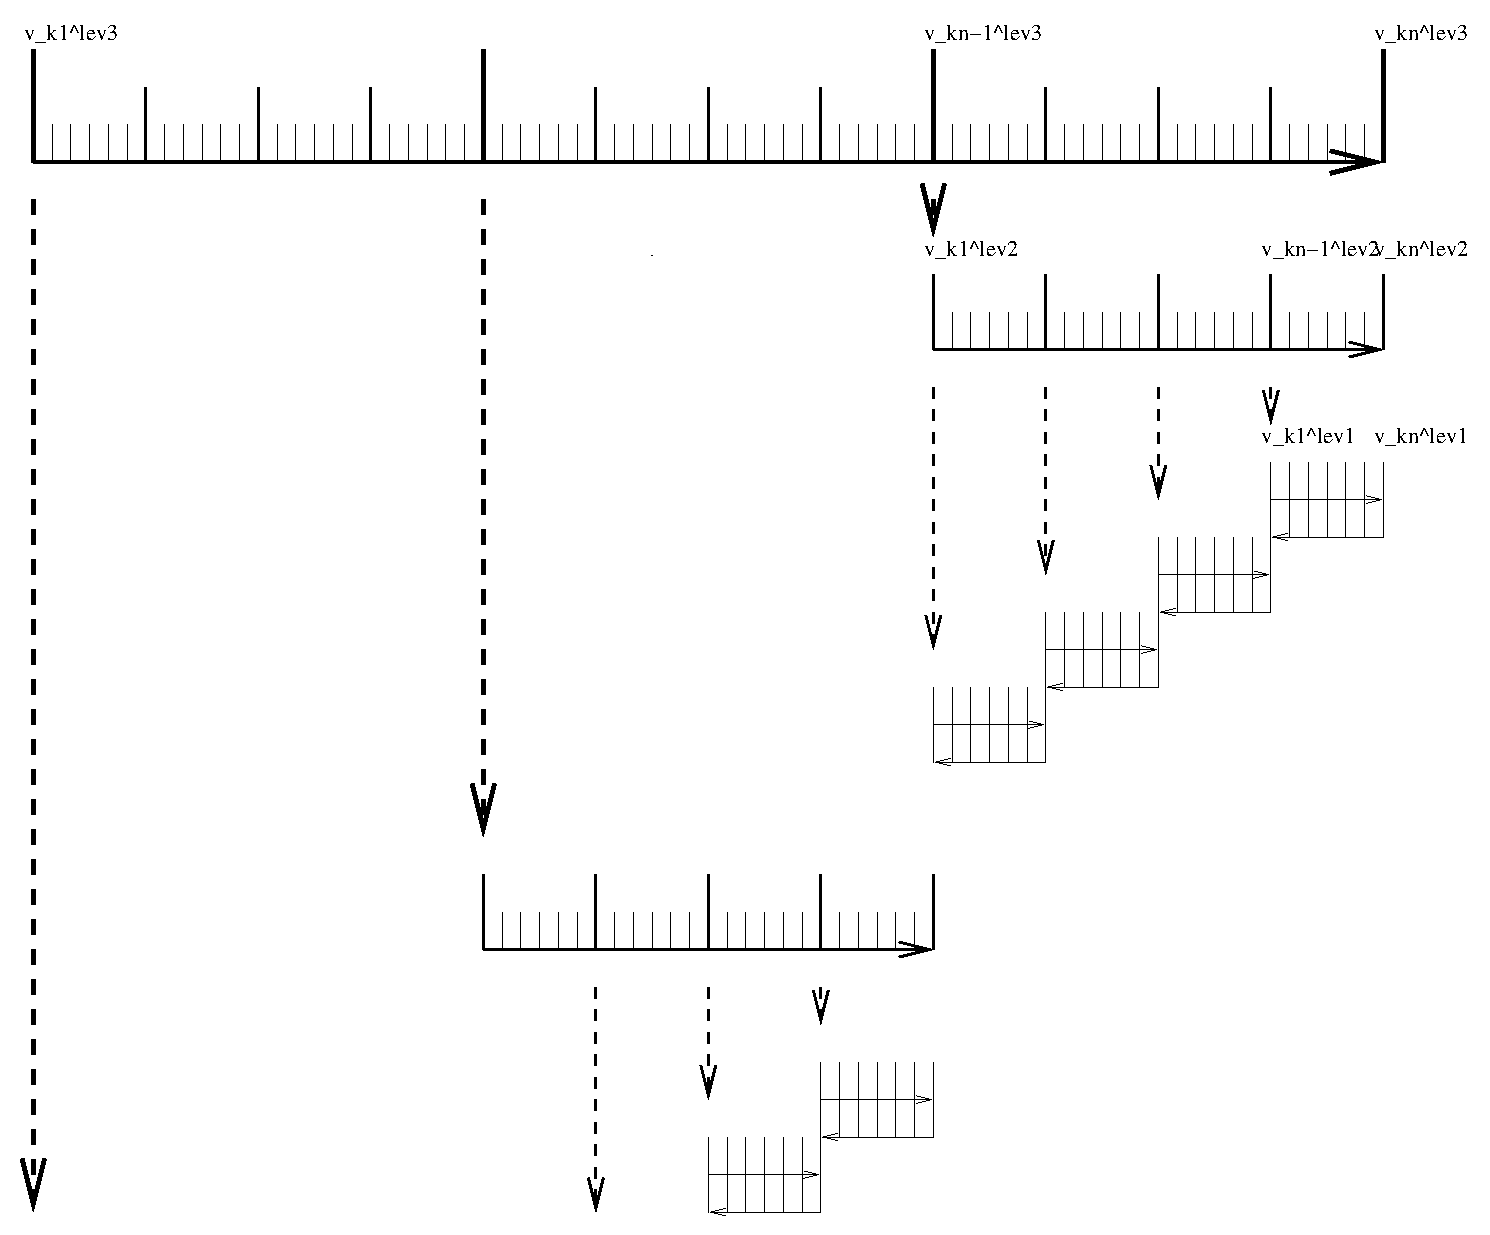
\epsfig{file=part5/checkpointing.eps, width=0.8\textwidth}}
\resizebox{5.5in}{!}{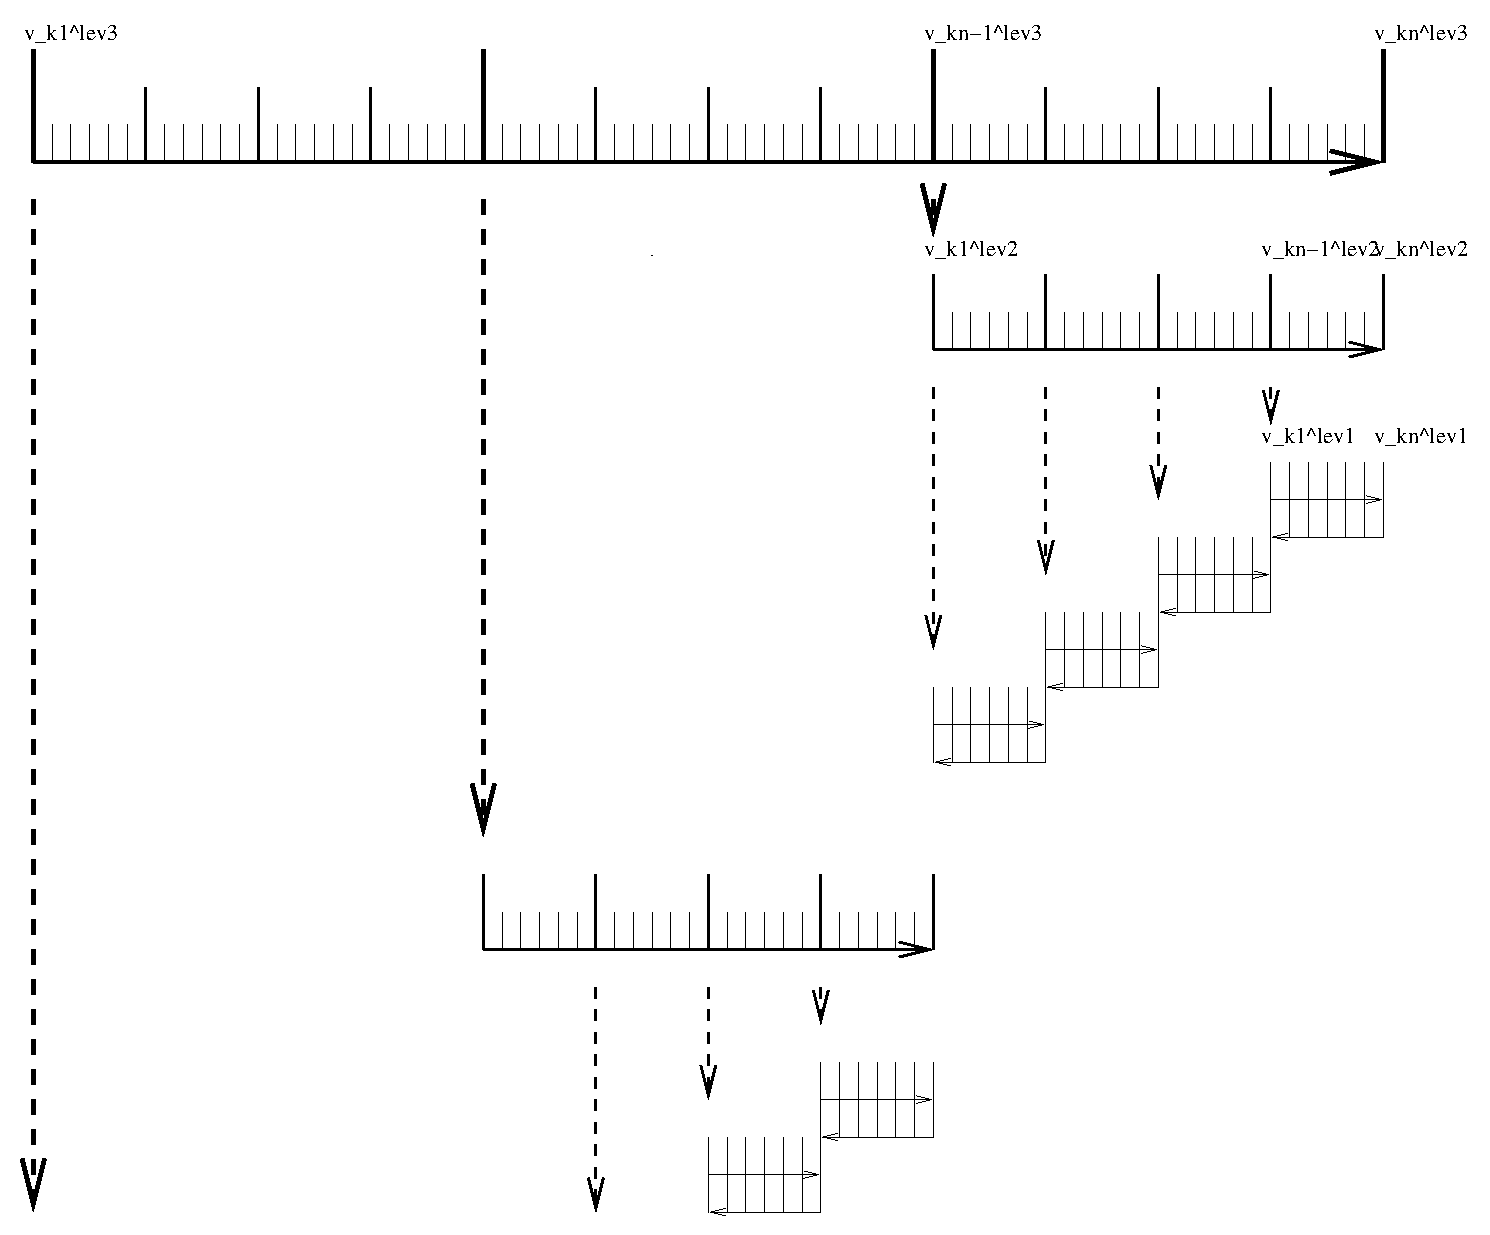
\includegraphics{part5/checkpointing.eps}}
%\psfull
\end{center}
\caption{
Schematic view of intermediate dump and restart for 
3-level checkpointing.}
\label{fig:3levelcheck}
\end{figure}

% \subsection{Optimal perturbations}
% \label{sec_optpert}


% \subsection{Error covariance estimate and Hessian matrix}
% \label{sec_hessian}

\newpage 

%**********************************************************************
\section{TLM and ADM generation in general}
\label{sec_ad_setup_gen}
%**********************************************************************

In this section we describe in a general fashion 
the parts of the code that are relevant for automatic
differentiation using the software tool TAMC. 

% $Header: /u/gcmpack/manual/s_autodiff/text/doc_ad_the_model.tex,v 1.3 2001/11/15 15:05:45 cnh Exp $
% $Name:  $
\begin{figure}[b!]

{\scriptsize
\begin{verbatim}
   the_model_main
   |
   |--- initialise_fixed
   |
   |--- #ifdef ALLOW_ADJOINT_RUN
   |           |    
   |           |--- ctrl_unpack
   |           |    
   |           |--- adthe_main_loop
   |           |    |
   |           |    |--- initialise_varia
   |           |    |--- ctrl_map_forcing
   |           |    |--- do iloop = 1, nTimeSteps
   |           |    |       |--- forward_step
   |           |    |       |--- cost_tile
   |           |    |    end do
   |           |    |--- cost_final
   |           |    |
   |           |    |--- adcost_final
   |           |    |--- do iloop = nTimeSteps, 1, -1
   |           |    |       |--- adcost_tile
   |           |    |       |--- adforward_step
   |           |    |    end do
   |           |    |--- adctrl_map_forcing
   |           |    |--- adinitialise_varia
   |           |    o
   |           |
   |           |--- ctrl_pack
   |           |
   |--- #else
   |           |
   |           |--- the_main_loop
   |           |
   |    #endif
   |
   |--- #ifdef ALLOW_GRADIENT_CHECK
   |           |
   |           |--- grdchk_main
   |           o
   |    #endif
   o
\end{verbatim}
}
\caption{~}
\label{fig:adthemodel}
\end{figure}



The basic flow is depicted in \ref{fig:adthemodel}.
If the option {\tt ALLOW\_AUTODIFF\_TAMC} is defined, the driver routine
{\it the\_model\_main}, instead of calling {\it the\_main\_loop},
invokes the adjoint of this routine, {\it adthe\_main\_loop},
which is the toplevel routine in terms of reverse mode computation.
The routine {\it adthe\_main\_loop} has been generated by TAMC.
It contains both the forward integration of the full model, 
any additional storing that is required for efficient checkpointing, 
and the reverse integration of the adjoint model.
The structure of {\it adthe\_main\_loop} has been strongly
simplified for clarification; in particular, no checkpointing
procedures are shown here.
Prior to the call of {\it adthe\_main\_loop}, the routine
{\it ctrl\_unpack} is invoked to unpack the control vector
or initialise the control variables.
Following the call of {\it adthe\_main\_loop}, 
the routine {\it ctrl\_pack}
is invoked to pack the control vector
(cf. Section \ref{section_ctrl}).
If gradient checks are to be performed, the option 
{\tt ALLOW\_GRADIENT\_CHECK} is defined. In this case
the driver routine {\it grdchk\_main} is called after
the gradient has been computed via the adjoint
(cf. Section \ref{section_grdchk}).

\subsection{The cost function (dependent variable)
\label{section_cost}}

The cost function $ {\cal J} $ is referred to as the {\sf dependent variable}.
It is a function of the input variables $ \vec{u} $ via the composition
$ {\cal J}(\vec{u}) \, = \, {\cal J}(M(\vec{u})) $. 
The input are referred to as the
{\sf independent variables} or {\sf control variables}.
All aspects relevant to the treatment of the cost function $ {\cal J} $
(parameter setting, initialization, accumulation, 
final evaluation), are controlled by the package {\it pkg/cost}.
The aspects relevant to the treatment of the independent variables
are controlled by the package {\it pkg/ctrl} and will be treated
in the next section.

\begin{figure}[!ht]

{\scriptsize
\begin{verbatim}
      the_model_main
      |
      |-- initialise_fixed
      |   |
      |   |-- packages_readparms
      |       |
      |       |-- cost_readparms
      |       o
      |
      |-- the_main_loop
     ...  |
          |-- initialise_varia
          |   |
          |   |-- packages_init_variables
          |       |
          |       |-- cost_init
          |       o
          |
          |-- do iloop = 1,nTimeSteps
          |      |-- forward_step
          |      |-- cost_tile
          |      |   |
          |      |   |-- cost_tracer
          |   end do
          |
          |-- cost_final
          o
\end{verbatim}
}

\caption{~}
\label{fig:costflow}
\end{figure}


\subsubsection{genmake and CPP options}
%
\begin{itemize}
%
\item 
\fbox{
\begin{minipage}{12cm}
{\it genmake}, {\it CPP\_OPTIONS.h}, {\it ECCO\_CPPOPTIONS.h}
\end{minipage}
}
\end{itemize}
%
The directory {\it pkg/cost} can be included to the
compile list in 3 different ways (cf. Section \ref{???}):
%
\begin{enumerate}
%
\item {\it genmake}: \\
Change the default settings in the file {\it genmake} by adding 
{\bf cost} to the {\bf enable} list (not recommended).
%
\item {\it .genmakerc}: \\
Customize the settings of {\bf enable}, {\bf disable} which are
appropriate for your experiment in the file {\it .genmakerc} 
and add the file to your compile directory.
%
\item genmake-options: \\
Call {\it genmake} with the option
{\tt genmake -enable=cost}.
%
\end{enumerate}
N.B.: In general the following packages ought to be enabled
simultaneously: {\it autodiff, cost, ctrl}.
The basic CPP option to enable the cost function is {\bf ALLOW\_COST}.
Each specific cost function contribution has its own option.
For the present example the option is {\bf ALLOW\_COST\_TRACER}.
All cost-specific options are set in {\it ECCO\_CPPOPTIONS.h}
Since the cost function is usually used in conjunction with
automatic differentiation, the CPP option
{\bf ALLOW\_ADJOINT\_RUN} (file {\it CPP\_OPTIONS.h}) and
{\bf ALLOW\_AUTODIFF\_TAMC} (file {\it ECCO\_CPPOPTIONS.h})
should be defined.

\subsubsection{Initialization}
%
The initialization of the {\it cost} package is readily enabled
as soon as the CPP option {\bf ALLOW\_COST} is defined.
%
\begin{itemize}
%
\item 
\fbox{
\begin{minipage}{12cm}
Parameters: {\it cost\_readparms}
\end{minipage}
}
\\
This S/R 
reads runtime flags and parameters from file {\it data.cost}.
For the present example the only relevant parameter read
is {\bf mult\_tracer}. This multiplier enables different
cost function contributions to be switched on
( = 1.) or off ( = 0.) at runtime.
For more complex cost functions which involve model vs. data
misfits, the corresponding data filenames and data
specifications (start date and time, period, ...) are read
in this S/R.
%
\item 
\fbox{
\begin{minipage}{12cm}
Variables: {\it cost\_init}
\end{minipage}
}
\\
This S/R 
initializes the different cost function contributions.
The contribution for the present example is {\bf objf\_tracer}
which is defined on each tile (bi,bj).
%
\end{itemize}
%
\subsubsection{Accumulation}
%
\begin{itemize}
%
\item 
\fbox{
\begin{minipage}{12cm}
{\it cost\_tile}, {\it cost\_tracer}
\end{minipage}
}
\end{itemize}
%
The 'driver' routine
{\it cost\_tile} is called at the end of each time step.
Within this 'driver' routine, S/R are called for each of
the chosen cost function contributions.
In the present example ({\bf ALLOW\_COST\_TRACER}),
S/R {\it cost\_tracer} is called.
It accumulates {\bf objf\_tracer} according to eqn. (\ref{???}).
%
\subsubsection{Finalize all contributions}
%
\begin{itemize}
%
\item 
\fbox{
\begin{minipage}{12cm}
{\it cost\_final}
\end{minipage}
}
\end{itemize}
%
At the end of the forward integration S/R {\it cost\_final}
is called. It accumulates the total cost function {\bf fc}
from each contribution and sums over all tiles:
\begin{equation}
{\cal J} \, = \, 
{\rm fc} \, = \, 
{\rm mult\_tracer} \sum_{\text{global sum}} \sum_{bi,\,bj}^{nSx,\,nSy}
{\rm objf\_tracer}(bi,bj) \, + \, ...
\end{equation}
%
The total cost function {\bf fc} will be the
'dependent' variable in the argument list for TAMC, i.e.
\begin{verbatim}
tamc -output 'fc' ...
\end{verbatim}

%%%% \end{document}

% $Header: /u/gcmpack/manual/s_autodiff/text/doc_ad_the_main.tex,v 1.3 2001/11/15 16:57:48 cnh Exp $
% $Name:  $
\begin{figure}

{\scriptsize
\begin{verbatim}
   *************
   the_main_loop
   *************
   |
   |--- initialise_varia
   |    |
   |   ...
   |    |--- packages_init_varia
   |    |    |
   |    |   ...
   |    |    |--- #ifdef ALLOW_ADJOINT_RUN
   |    |    |          call ctrl_map_ini
   |    |    |          call cost_ini
   |    |    |    #endif
   |    |   ...
   |    |    o
   |   ...
   |    o
  ...
   |--- #ifdef ALLOW_ADJOINT_RUN
   |          call ctrl_map_forcing
   |    #endif
  ...
   |--- #ifdef ALLOW_TAMC_CHECKPOINTING
              do ilev_3 = 1,nchklev_3
   |            do ilev_2 = 1,nchklev_2
   |              do ilev_1 = 1,nchklev_1
   |                iloop = (ilev_3-1)*nchklev_2*nchklev_1 +
   |                        (ilev_2-1)*nchklev_1           + ilev_1
   |    #else
   |          do iloop = 1, nTimeSteps
   |    #endif
   |    |
   |    |---       call forward_step
   |    |
   |    |--- #ifdef ALLOW_COST
   |    |          call cost_tile
   |    |    #endif
   |    |
   |    |    enddo
   |    o
   |
   |--- #ifdef ALLOW_COST
   |          call cost_final
   |    #endif
   o
\end{verbatim}
}
\caption{~}
\label{fig:adthemain}
\end{figure}


\subsection{The control variables (independent variables)
\label{section_ctrl}}

The control variables are a subset of the model input
(initial conditions, boundary conditions, model parameters).
Here we identify them with the variable $ \vec{u} $.
All intermediate variables whose derivative w.r.t. control
variables do not vanish are called {\sf active variables}.
All subroutines whose derivative w.r.t. the control variables
don't vanish are called {\sf active routines}.
Read and write operations from and to file can be viewed
as variable assignments. Therefore, files to which
active variables are written and from which active variables
are read are called {\sf active files}.
All aspects relevant to the treatment of the control variables
(parameter setting, initialization, perturbation)
are controlled by the package {\it pkg/ctrl}.

\begin{figure}[h!]

{\scriptsize
\begin{verbatim}
          the_model_main
          |
          |-- initialise_fixed
          |   |
          |   |-- packages_readparms
          |       |
          |       |-- ctrl_init                - initialise control
          |       o                              package
          |
          |-- ctrl_unpack                      - unpack control vector
          |
          |-- adthe_main_loop                  - forward/adjoint run
          |   |
          |   |-- initialise_variables
          |   |   |
          |   |   |-- packages_init_variables
          |   |       |
          |   |       |-- ctrl_map_ini         - link init. state and
          |   |       o                          parameters to control 
          |   |                                  variables
          |   |-- ctrl_map_forcing             - link forcing fields to
          |  ...                                 control variables
          |
          |-- ctrl_pack                        - pack control vector
\end{verbatim}
}
\caption{~}
\label{fig:ctrlflow}
\end{figure}


\subsubsection{genmake and CPP options}
%
\begin{itemize}
%
\item 
\fbox{
\begin{minipage}{12cm}
{\it genmake}, {\it CPP\_OPTIONS.h}, {\it ECCO\_CPPOPTIONS.h}
\end{minipage}
}
\end{itemize}
%
To enable the directory to be included to the compile list,
{\bf ctrl} has to be added to the {\bf enable} list in
{\it .genmakerc} or in {\it genmake} itself (analogous to {\it cost}
package, cf. previous section).
Each control variable is enabled via its own CPP option
in {\it ECCO\_CPPOPTIONS.h}.

\subsubsection{Initialization}
%
\begin{itemize}
%
\item 
\fbox{
\begin{minipage}{12cm}
Parameters: {\it ctrl\_readparms}
\end{minipage}
}
\\
%
This S/R 
reads runtime flags and parameters from file {\it data.ctrl}.
For the present example the file contains the file names
of each control variable that is used.
In addition, the number of wet points for each control
variable and the net dimension of the space of control
variables (counting wet points only) {\bf nvarlength}
is determined.
Masks for wet points for each tile {\bf (bi,\,bj)}
and vertical layer {\bf k} are generated for the three
relevant categories on the C-grid:
{\bf nWetCtile} for tracer fields, 
{\bf nWetWtile} for zonal velocity fields,
{\bf nWetStile} for meridional velocity fields.
%
\item 
\fbox{
\begin{minipage}{12cm}
Control variables, control vector,
and their gradients: {\it ctrl\_unpack}
\end{minipage}
}
\\
%
Two important issues related to the handling of the control
variables in the MITGCM need to be addressed.
First, in order to save memory, the control variable arrays
are not kept in memory, but rather read from file and added
to the initial fields during the model initialization phase.
Similarly, the corresponding adjoint fields which represent
the gradient of the cost function w.r.t. the control variables
are written to file at the end of the adjoint integration.
Second, in addition to the files holding the 2-dim. and 3-dim.
control variables and the corresponding cost gradients, 
a 1-dim. {\sf control vector} 
and {\sf gradient vector} are written to file. They contain 
only the wet points of the control variables and the corresponding 
gradient.
This leads to a significant data compression.
Furthermore, an option is available
({\tt ALLOW\_NONDIMENSIONAL\_CONTROL\_IO}) to
non-dimensionalise the control and gradient vector,
which otherwise would contain different pieces of different
magnitudes and units.
Finally, the control and gradient vector can be passed to a 
minimization routine if an update of the control variables
is sought as part of a minimization exercise.

The files holding fields and vectors of the control variables
and gradient are generated and initialised in S/R {\it ctrl\_unpack}.
%
\end{itemize}

\subsubsection{Perturbation of the independent variables}
%
The dependency flow for differentiation w.r.t. the controls 
starts with adding a perturbation onto the input variable,
thus defining the independent or control variables for TAMC.
Three types of controls may be considered:
%
\begin{itemize}
%
\item 
\fbox{
\begin{minipage}{12cm}
{\it ctrl\_map\_ini} (initial value sensitivity): 
\end{minipage}
}
\\
%
Consider as an example the initial tracer distribution
{\bf tr1} as control variable.
After {\bf tr1} has been initialised in
{\it ini\_tr1} (dynamical variables such as
temperature and salinity are initialised in {\it ini\_fields}),
a perturbation anomaly is added to the field in S/R
{\it ctrl\_map\_ini}
%
\begin{equation}
\begin{split}
u         & = \, u_{[0]} \, + \, \Delta u \\
{\bf tr1}(...) & = \, {\bf tr1_{ini}}(...) \, + \, {\bf xx\_tr1}(...)
\label{perturb}
\end{split}
\end{equation}
%
{\bf xx\_tr1} is a 3-dim. global array 
holding the perturbation. In the case of a simple
sensitivity study this array is identical to zero.
However, it's specification is essential in the context
of automatic differentiation since TAMC
treats the corresponding line in the code symbolically
when determining the differentiation chain and its origin.
Thus, the variable names are part of the argument list
when calling TAMC: 
%
\begin{verbatim}
tamc -input 'xx_tr1 ...' ...
\end{verbatim}
%
Now, as mentioned above, the MITGCM avoids maintaining
an array for each control variable by reading the
perturbation to a temporary array from file.
To ensure the symbolic link to be recognized by TAMC, a scalar
dummy variable {\bf xx\_tr1\_dummy} is introduced
and an 'active read' routine of the adjoint support
package {\it pkg/autodiff} is invoked.
The read-procedure is tagged with the variable
{\bf xx\_tr1\_dummy} enabling TAMC to recognize the
initialization of the perturbation.
The modified call of TAMC thus reads
%
\begin{verbatim}
tamc -input 'xx_tr1_dummy ...' ...
\end{verbatim}
%
and the modified operation to (\ref{perturb})
in the code takes on the form
%
\begin{verbatim}
       call active_read_xyz( 
     &      ..., tmpfld3d, ..., xx_tr1_dummy, ... )

       tr1(...) = tr1(...) + tmpfld3d(...)
\end{verbatim}
%
Note, that reading an active variable corresponds
to a variable assignment. Its derivative corresponds
to a write statement of the adjoint variable, followed by
a reset.
The 'active file' routines have been designed
to support active read and corresponding adjoint active write
operations (and vice versa).
%
\item 
\fbox{
\begin{minipage}{12cm}
{\it ctrl\_map\_forcing} (boundary value sensitivity): 
\end{minipage}
}
\\
%
The handling of boundary values as control variables
proceeds exactly analogous to the initial values
with the symbolic perturbation taking place in S/R
{\it ctrl\_map\_forcing}.
Note however an important difference:
Since the boundary values are time dependent with a new
forcing field applied at each time steps,
the general problem may be thought of as
a new control variable at each time step
(or, if the perturbation is averaged over a certain period,
at each $ N $ timesteps), i.e.
\[
u_{\rm forcing} \, = \,
\{ \, u_{\rm forcing} ( t_n ) \, \}_{
n \, = \, 1, \ldots , {\rm nTimeSteps} }
\]
%
In the current example an equilibrium state is considered,
and only an initial perturbation to
surface forcing is applied with respect to the
equilibrium state.
A time dependent treatment of the surface forcing is 
implemented in the ECCO environment, involving the
calendar ({\it cal}~) and external forcing ({\it exf}~) packages.
%
\item 
\fbox{
\begin{minipage}{12cm}
{\it ctrl\_map\_params} (parameter sensitivity): 
\end{minipage}
}
\\
%
This routine is not yet implemented, but would proceed
proceed along the same lines as the initial value sensitivity.
The mixing parameters {\bf diffkr} and {\bf kapgm}
are currently added as controls in {\it ctrl\_map\_ini.F}.
%
\end{itemize}
%

\subsubsection{Output of adjoint variables and gradient}
%
Several ways exist to generate output of adjoint fields.
%
\begin{itemize}
%
\item 
\fbox{
\begin{minipage}{12cm}
{\it ctrl\_map\_ini, ctrl\_map\_forcing}: 
\end{minipage}
}
\\
\begin{itemize}
%
\item {\bf xx\_...}: the control variable fields \\
Before the forward integration, the control
variables are read from file {\bf xx\_ ...} and added to
the model field.
%
\item {\bf adxx\_...}: the adjoint variable fields, i.e. the gradient
$ \nabla _{u}{\cal J} $ for each control variable \\
After the adjoint integration the corresponding adjoint
variables are written to {\bf adxx\_ ...}.
%
\end{itemize}
%
\item 
\fbox{
\begin{minipage}{12cm}
{\it ctrl\_unpack, ctrl\_pack}: 
\end{minipage}
}
\\
%
\begin{itemize}
%
\item {\bf vector\_ctrl}: the control vector \\
At the very beginning of the model initialization,
the updated compressed control vector is read (or initialised)
and distributed to 2-dim. and 3-dim. control variable fields.
%
\item {\bf vector\_grad}: the gradient vector \\
At the very end of the adjoint integration,
the 2-dim. and 3-dim. adjoint variables are read,
compressed to a single vector and written to file.
%
\end{itemize}
%
\item 
\fbox{
\begin{minipage}{12cm}
{\it addummy\_in\_stepping}: 
\end{minipage}
}
\\
In addition to writing the gradient at the end of the
forward/adjoint integration, many more adjoint variables
of the model state
at intermediate times can be written using S/R 
{\it addummy\_in\_stepping}.
This routine is part of the adjoint support package 
{\it pkg/autodiff} (cf.f. below).
The procedure is enabled using via the CPP-option
{\bf ALLOW\_AUTODIFF\_MONITOR} (file {\it ECCO\_CPPOPTIONS.h}).
To be part of the adjoint code, the corresponding S/R
{\it dummy\_in\_stepping} has to be called in the forward
model (S/R {\it the\_main\_loop}) at the appropriate place.
The adjoint common blocks are extracted from the adjoint code
via the header file {\it adcommon.h}.

{\it dummy\_in\_stepping} is essentially empty,
the corresponding adjoint routine is hand-written rather
than generated automatically.
Appropriate flow directives ({\it dummy\_in\_stepping.flow})
ensure that TAMC does not automatically 
generate {\it addummy\_in\_stepping} by trying to differentiate
{\it dummy\_in\_stepping}, but instead refers to 
the hand-written routine.

{\it dummy\_in\_stepping} is called in the forward code
at the beginning of each
timestep, before the call to {\it dynamics}, thus ensuring
that {\it addummy\_in\_stepping} is called at the end of
each timestep in the adjoint calculation, after the call to
{\it addynamics}.

{\it addummy\_in\_stepping} includes the header files
{\it adcommon.h}.
This header file is also hand-written. It contains
the common blocks 
{\bf /addynvars\_r/}, {\bf /addynvars\_cd/},
{\bf /addynvars\_diffkr/}, {\bf /addynvars\_kapgm/},
{\bf /adtr1\_r/}, {\bf /adffields/},
which have been extracted from the adjoint code to enable
access to the adjoint variables.

{\bf WARNING:} If the structure of the common blocks
{\bf /dynvars\_r/}, {\bf /dynvars\_cd/}, etc., changes
similar changes will occur in the adjoint common blocks.
Therefore, consistency between the TAMC-generated common blocks
and those in {\it adcommon.h} have to be checked.
%
\end{itemize}


\subsubsection{Control variable handling for 
optimization applications}

In optimization mode the cost function $ {\cal J}(u) $ is sought
to be minimized with respect to a set of control variables
$ \delta {\cal J} \, = \, 0 $, in an iterative manner.
The gradient $ \nabla _{u}{\cal J} |_{u_{[k]}} $ together
with the value of the cost function itself $ {\cal J}(u_{[k]}) $ 
at iteration step $ k $ serve
as input to a minimization routine (e.g. quasi-Newton method,
conjugate gradient, ... \cite{gil-lem:89}) 
to compute an update in the
control variable for iteration step $k+1$
\[
u_{[k+1]} \, = \,  u_{[0]} \, + \, \Delta u_{[k+1]}
\quad \mbox{satisfying} \quad
 {\cal J} \left( u_{[k+1]} \right) \, < \, {\cal J} \left( u_{[k]} \right)
\]
$ u_{[k+1]} $ then serves as input for a forward/adjoint run
to determine $ {\cal J} $ and $ \nabla _{u}{\cal J} $ at iteration step
$ k+1 $.
Tab. \ref{???} sketches the flow between forward/adjoint model
and the minimization routine.

\begin{eqnarray*}
\scriptsize
\begin{array}{ccccc}
u_{[0]} \,\, ,  \,\, \Delta u_{[k]}    & ~ & ~ & ~ & ~ \\
{\Big\downarrow} 
   & ~ & ~ & ~ & ~ \\
 ~ & ~ & ~ & ~ & ~ \\
\hline
\multicolumn{1}{|c}{~} & ~ & ~ & ~ & \multicolumn{1}{c|}{~} \\
\multicolumn{1}{|c}{
u_{[k]} = u_{[0]} + \Delta u_{[k]}} &
\stackrel{\bf forward}{\bf \longrightarrow} &
v_{[k]} = M \left( u_{[k]} \right) &
\stackrel{\bf forward}{\bf \longrightarrow} &
\multicolumn{1}{c|}{
{\cal J}_{[k]} = {\cal J} \left( M \left( u_{[k]} \right) \right)} \\
\multicolumn{1}{|c}{~} & ~ & ~ & ~ & \multicolumn{1}{c|}{~} \\
\hline
\multicolumn{1}{|c}{~} & ~ & ~ & ~ & \multicolumn{1}{c|}{~}  \\
\multicolumn{1}{|c}{~} & ~ & ~ & ~ & \multicolumn{1}{c|}{{\Big\downarrow}} \\
\multicolumn{1}{|c}{~} & ~ & ~ & ~ & \multicolumn{1}{c|}{~}  \\
\hline
\multicolumn{1}{|c}{~} & ~ & ~ & ~ & \multicolumn{1}{c|}{~} \\
\multicolumn{1}{|c}{
\nabla_u {\cal J}_{[k]} (\delta {\cal J}) = 
T^{\ast} \cdot \nabla_v {\cal J} |_{v_{[k]}} (\delta {\cal J})} &
\stackrel{\bf adjoint}{\mathbf \longleftarrow} &
ad \, v_{[k]} (\delta {\cal J}) = 
\nabla_v {\cal J} |_{v_{[k]}} (\delta {\cal J}) &
\stackrel{\bf adjoint}{\mathbf \longleftarrow} &
\multicolumn{1}{c|}{ ad \, {\cal J} = \delta {\cal J}} \\
\multicolumn{1}{|c}{~} & ~ & ~ & ~ & \multicolumn{1}{c|}{~} \\
\hline
 ~ & ~ & ~ & ~ & ~ \\
\hspace*{15ex}{\Bigg\downarrow}  
\quad {\cal J}_{[k]}, \quad \nabla_u {\cal J}_{[k]}
 & ~ & ~ & ~ & ~ \\
 ~ & ~ & ~ & ~ & ~ \\
\hline
\multicolumn{1}{|c}{~} & ~ & ~ & ~ & \multicolumn{1}{c|}{~} \\
\multicolumn{1}{|c}{
{\cal J}_{[k]} \,\, ,  \,\, \nabla_u {\cal J}_{[k]}} &
{\mathbf \longrightarrow} & \text{\bf minimisation} &
{\mathbf \longrightarrow} & 
\multicolumn{1}{c|}{ \Delta u_{[k+1]}} \\
\multicolumn{1}{|c}{~} & ~ & ~ & ~ & \multicolumn{1}{c|}{~} \\
\hline
 ~ & ~ & ~ & ~ & ~ \\
 ~ & ~ & ~ & ~ & \Big\downarrow \\
 ~ & ~ & ~ & ~ & \Delta u_{[k+1]} \\
\end{array}
\end{eqnarray*}

The routines {\it ctrl\_unpack} and {\it ctrl\_pack} provide
the link between the model and the minimization routine.
As described in Section \ref{???} 
the {\it unpack} and {\it pack} routines read and write
control and gradient {\it vectors} which are compressed
to contain only wet points, in addition to the full
2-dim. and 3-dim. fields. 
The corresponding I/O flow looks as follows:

\vspace*{0.5cm}

{\scriptsize
\begin{tabular}{ccccc}
{\bf vector\_ctrl\_$<$k$>$ } & ~ & ~ & ~ & ~ \\
{\big\downarrow}  & ~ & ~ & ~ & ~ \\
\cline{1-1}
\multicolumn{1}{|c|}{\it ctrl\_unpack} & ~ & ~ & ~ & ~ \\
\cline{1-1}
{\big\downarrow}  & ~ & ~ & ~ & ~ \\
\cline{3-3}
\multicolumn{1}{l}{\bf xx\_theta0...$<$k$>$} & ~ &
\multicolumn{1}{|c|}{~} & ~ & ~ \\
\multicolumn{1}{l}{\bf xx\_salt0...$<$k$>$} & 
$\stackrel{\mbox{read}}{\longrightarrow}$ &
\multicolumn{1}{|c|}{forward integration} & ~ & ~ \\ 
\multicolumn{1}{l}{\bf \vdots} & ~ & \multicolumn{1}{|c|}{~}  
& ~ & ~ \\
\cline{3-3}
~ & ~ & $\downarrow$ & ~ & ~ \\
\cline{3-3}
~ & ~ & 
\multicolumn{1}{|c|}{~} & ~ & 
\multicolumn{1}{l}{\bf adxx\_theta0...$<$k$>$}  \\
~ & ~ & \multicolumn{1}{|c|}{adjoint integration} & 
$\stackrel{\mbox{write}}{\longrightarrow}$ & 
\multicolumn{1}{l}{\bf adxx\_salt0...$<$k$>$} \\ 
~ & ~ & \multicolumn{1}{|c|}{~}  
& ~ & \multicolumn{1}{l}{\bf \vdots} \\
\cline{3-3}
~ & ~ & ~ & ~ & {\big\downarrow} \\
\cline{5-5}
~ & ~ & ~ & ~ & \multicolumn{1}{|c|}{\it ctrl\_pack} \\
\cline{5-5}
~ & ~ & ~ & ~ &  {\big\downarrow} \\
~ & ~ & ~ & ~ &  {\bf vector\_grad\_$<$k$>$ } \\
\end{tabular}
}

\vspace*{0.5cm}


{\it ctrl\_unpack} reads the updated control vector
{\bf vector\_ctrl\_$<$k$>$}.
It distributes the different control variables to
2-dim. and 3-dim. files {\it xx\_...$<$k$>$}.
At the start of the forward integration the control variables
are read from {\it xx\_...$<$k$>$} and added to the
field.
Correspondingly, at the end of the adjoint integration
the adjoint fields are written
to {\it adxx\_...$<$k$>$}, again via the active file routines.
Finally, {\it ctrl\_pack} collects all adjoint files
and writes them to the compressed vector file
{\bf vector\_grad\_$<$k$>$}.


\newpage
%\chapter{Tutorial III - Differentiated Code}
%\label{chap:tutorialIII}

% moved to part 3 % $Header: /u/gcmpack/manual/s_autodiff/Attic/doc_ad_examples.tex,v 1.2 2002/04/24 11:01:47 heimbach Exp $
% $Name:  $

%**********************************************************************
\section{Sensitivity of Air-Sea Exchange to Tracer Injection Site }
\label{sect:eg-simple-tracer-adjoint}
\label{sec_ad_setup_ex}
%**********************************************************************

The MITGCM has been adapted to enable AD using TAMC or TAF.
The present description, therefore, is specific to the
use of TAMC or TAF as AD tool.
The following sections describe the steps which are necessary to 
generate a tangent linear or adjoint model of the MITGCM.
We take as an example the sensitivity of carbon sequestration
in the ocean.
The AD-relevant hooks in the code are sketched in 
\ref{fig:adthemodel}, \ref{fig:adthemain}.

\subsection{Overview of the experiment}

We describe an adjoint sensitivity analysis of out-gassing from 
the ocean into the atmosphere of a carbon-like tracer injected
into the ocean interior (see \cite{hil-eta:01}).

\subsubsection{Passive tracer equation}

For this work the MITGCM was augmented with a thermodynamically 
inactive tracer, $C$. Tracer residing in the ocean 
model surface layer is out-gassed according to a relaxation time scale, 
$\mu$. Within the ocean interior, the tracer is passively advected 
by the ocean model currents. The full equation for the time evolution
%
\begin{equation}
\label{carbon_ddt}
\frac{\partial C}{\partial t} \, = \, 
-U\cdot \nabla C \, - \, \mu C \, + \, \Gamma(C) \,+ \, S
\end{equation}
%
also includes a source term $S$. This term 
represents interior sources of $C$ such as would arise due to
direct injection.
The velocity term, $U$, is the sum of the
model Eulerian circulation and an eddy-induced velocity, the latter
parameterized according to Gent/McWilliams 
(\cite{gen-mcw:90, gen-eta:95}).
The convection function, $\Gamma$, mixes $C$ vertically wherever the 
fluid is locally statically unstable. 

The out-gassing time scale, $\mu$, in eqn. (\ref{carbon_ddt})
is set so that \( 1/\mu \sim 1 \ \mathrm{year} \) for the surface
ocean and $\mu=0$ elsewhere. With this value, eqn. (\ref{carbon_ddt})
is valid as a prognostic equation for small perturbations in oceanic 
carbon concentrations. This configuration provides a 
powerful tool for examining the impact of large-scale ocean circulation
on $ CO_2 $ out-gassing due to interior injections.
As source we choose a constant in time injection of 
$ S = 1 \,\, {\rm mol / s}$.

\subsubsection{Model configuration}

The model configuration employed has a constant 
$4^\circ \times 4^\circ$ resolution horizontal grid and realistic 
geography and bathymetry. Twenty vertical layers are used with 
vertical spacing ranging
from 50 m near the surface to 815 m at depth. 
Driven to steady-state by climatological wind-stress, heat and
fresh-water forcing the model reproduces well known large-scale
features of the ocean general circulation. 

\subsubsection{Out-gassing cost function}

To quantify and understand out-gassing due to injections of $C$
in eqn. (\ref{carbon_ddt}),
we define a cost function $ {\cal J} $ that measures the total amount of 
tracer out-gassed at each timestep:
%
\begin{equation}
\label{cost_tracer}
{\cal J}(t=T)=\int_{t=0}^{t=T}\int_{A} \mu C \, dA \, dt
\end{equation}
%
Equation(\ref{cost_tracer}) integrates the out-gassing term, $\mu C$, 
from (\ref{carbon_ddt})
over the entire ocean surface area, $A$, and accumulates it 
up to time $T$.
Physically, ${\cal J}$ can be thought of as representing the amount of 
$CO_2$ that our model predicts would be out-gassed following an
injection at rate $S$.
The sensitivity of ${\cal J}$ to the spatial location of $S$, 
$\frac{\partial {\cal J}}{\partial S}$,
can be used to identify regions from which circulation
would cause $CO_2$ to rapidly out-gas following injection
and regions in which $CO_2$ injections would remain effectively 
sequestered within the ocean.

\subsection{Code configuration}

The model configuration for this experiment resides under the
directory {\it verification/carbon/}.
The code customization routines are in {\it verification/carbon/code/}:
%
\begin{itemize}
%
\item {\it .genmakerc}
%
\item {\it COST\_CPPOPTIONS.h}
%
\item {\it CPP\_EEOPTIONS.h}
%
\item {\it CPP\_OPTIONS.h}
%
\item {\it CTRL\_OPTIONS.h}
%
\item {\it ECCO\_OPTIONS.h}
%
\item {\it SIZE.h}
%
\item {\it adcommon.h}
%
\item {\it tamc.h}
%
\end{itemize}
%
The runtime flag and parameters settings are contained in 
{\it verification/carbon/input/},
together with the forcing fields and and restart files:
%
\begin{itemize}
%
\item {\it data}
%
\item {\it data.cost}
%
\item {\it data.ctrl}
%
\item {\it data.gmredi}
%
\item {\it data.grdchk}
%
\item {\it data.optim}
%
\item {\it data.pkg}
%
\item {\it eedata}
%
\item {\it topog.bin}
%
\item {\it windx.bin, windy.bin}
%
\item {\it salt.bin, theta.bin}
%
\item {\it SSS.bin, SST.bin}
%
\item {\it pickup*}
%
\end{itemize}
%
Finally, the file to generate the adjoint code resides in
$ adjoint/ $:
%
\begin{itemize}
%
\item {\it makefile}
%
\end{itemize}
%

Below we describe the customizations of this files which are
specific to this experiment.

\subsubsection{File {\it .genmakerc}}
This file overwrites default settings of {\it genmake}.
In the present example it is used to switch on the following
packages which are related to automatic differentiation
and are disabled by default: \\
\hspace*{4ex} {\tt set ENABLE=( autodiff cost ctrl ecco gmredi grdchk kpp )}  \\
Other packages which are not needed are switched off: \\
\hspace*{4ex} {\tt set DISABLE=( aim obcs zonal\_filt shap\_filt cal exf )}

\subsubsection{File {\it COST\_CPPOPTIONS.h,  CTRL\_OPTIONS.h}}

These files used to contain package-specific CPP-options
(see Section \ref{???}).
For technical reasons those options have been grouped together
in the file {\it ECCO\_OPTIONS.h}.
To retain the modularity, the files have been kept and contain
the standard include of the {\it CPP\_OPTIONS.h} file.

\subsubsection{File {\it CPP\_EEOPTIONS.h}}

This file contains 'wrapper'-specific CPP options.
It only needs to be changed if the code is to be run
in a parallel environment (see Section \ref{???}).

\subsubsection{File {\it CPP\_OPTIONS.h}}

This file contains model-specific CPP options
(see Section \ref{???}).
Most options are related to the forward model setup.
They are identical to the global steady circulation setup of
{\it verification/global\_ocean.90x40x15/}.
The three options specific to this experiment are \\
\hspace*{4ex} {\tt \#define ALLOW\_PASSIVE\_TRACER} \\
This flag enables the code to carry through the
advection/diffusion of a passive tracer along the
model integration. \\
\hspace*{4ex} {\tt \#define ALLOW\_MIT\_ADJOINT\_RUN} \\
This flag enables the inclusion of some AD-related fields
concerning initialization, link between control variables
and forward model variables, and the call to the top-level
forward/adjoint subroutine {\it adthe\_main\_loop}
instead of {\it the\_main\_loop}. \\
\hspace*{4ex} {\tt \#define ALLOW\_GRADIENT\_CHECK} \\
This flag enables the gradient check package.
After computing the unperturbed cost function and its gradient,
a series of computations are performed for which \\
$\bullet$ an element of the control vector is perturbed \\
$\bullet$ the cost function w.r.t. the perturbed element is
computed \\
$\bullet$ the difference between the perturbed and unperturbed
cost function is computed to compute the finite difference gradient \\
$\bullet$ the finite difference gradient is compared with the
adjoint-generated gradient.
The gradient check package is further described in Section ???.

\subsubsection{File {\it ECCO\_OPTIONS.h}}

The CPP options of several AD-related packages are grouped
in this file:
%
\begin{itemize}
%
\item 
Overall ECCO-related execution modus: \\
These determine whether a pure forward run,
a sensitivity run or an iteration of optimization is
performed. These options are not needed in the present context.
%
\item 
Adjoint support package: {\it pkg/autodiff/} \\
This package contains hand-written adjoint code such as
active file handling, flow directives for files which must not
be differentiated, and TAMC-specific header files. \\
%
\hspace*{4ex} {\tt \#define ALLOW\_AUTODIFF\_TAMC} \\
defines TAMC-related features in the code. \\
%
\hspace*{4ex} {\tt \#define ALLOW\_TAMC\_CHECKPOINTING} \\
enables the checkpointing feature of TAMC
(see Section \ref{???}).
In the present example a 3-level checkpointing is implemented.
The code contains the relevant store directives, common block
and tape initializations, storing key computation,
and loop index handling.
The checkpointing length at each level is defined in
file {\it tamc.h}, cf. below.
The out and intermediate loop directivs are contained
in the files {\it checkpoint\_lev3\_directives.h}, 
{\it checkpoint\_lev2\_directives.h} (package {\it pkg/autodiff}). \\
%
\hspace*{4ex} {\tt \#define ALLOW\_AUTODIFF\_MONITOOR} \\
enables the monitoring of intermediate adjoint variables
(see Section \ref{???}). \\
%
\hspace*{4ex} {\tt \#define ALLOW\_DIVIDED\_ADJOINT} \\
enables adjoint dump and restart
(see Section \ref{???}).
%
\item Cost function package: {\it pkg/cost/} \\
This package contains all relevant routines for
initializing, accumulating and finalizing the cost function
(see Section \ref{???}). \\
\hspace*{4ex} {\tt \#define ALLOW\_COST} \\
enables all general aspects of the cost function handling,
in particular the hooks in the forward code for
initializing, accumulating and finalizing the cost function. \\
\hspace*{4ex} {\tt \#define ALLOW\_COST\_TRACER} \\
includes the call to the cost function for this
particular experiment, eqn. (\ref{cost_tracer}).
%
\item Control variable package: {\it pkg/ctrl/} \\
This package contains all relevant routines for
the handling of the control vector.
Each control variable can be enabled/disabled with its own flag: \\
\begin{tabular}{ll}
\hspace*{2ex} {\tt \#define ALLOW\_THETA0\_CONTROL} & 
initial temperature \\
\hspace*{2ex} {\tt \#define ALLOW\_SALT0\_CONTROL} & 
initial salinity \\
\hspace*{2ex} {\tt \#define ALLOW\_TR0\_CONTROL} & 
initial passive tracer concentration \\
\hspace*{2ex} {\tt \#define ALLOW\_TAUU0\_CONTROL} & 
zonal wind stress \\
\hspace*{2ex} {\tt \#define ALLOW\_TAUV0\_CONTROL} & 
meridional wind stress \\
\hspace*{2ex} {\tt \#define ALLOW\_SFLUX0\_CONTROL} & 
freshwater flux \\
\hspace*{2ex} {\tt \#define ALLOW\_HFLUX0\_CONTROL} & 
heat flux \\
\hspace*{2ex} {\tt \#define ALLOW\_DIFFKR\_CONTROL} & 
diapycnal diffusivity \\
\hspace*{2ex} {\tt \#undef ALLOW\_KAPPAGM\_CONTROL} & 
isopycnal diffusivity \\
\end{tabular}
%
\end{itemize}

\subsubsection{File {\it SIZE.h}}

The file contains the grid point dimensions of the forward
model. It is identical to the {\it verification/exp2/}: \\
\hspace*{4ex} {\tt sNx = 90} \\
\hspace*{4ex} {\tt sNy = 40} \\
\hspace*{4ex} {\tt Nr = 20} \\
It corresponds to a single-tile/single-processor setup:
{\tt nSx = nSy = 1, nPx = nPy = 1},
with standard overlap dimensioning
{\tt OLx = OLy = 3}.

\subsubsection{File {\it adcommon.h}}

This file contains common blocks of some adjoint variables
that are generated by TAMC. 
The common blocks are used by the adjoint support routine
{\it addummy\_in\_stepping} which needs to access those variables:

\begin{tabular}{ll}
\hspace*{4ex} {\tt common /addynvars\_r/} &
\hspace*{4ex} is related to {\it DYNVARS.h} \\
\hspace*{4ex} {\tt common /addynvars\_cd/} &
\hspace*{4ex} is related to {\it DYNVARS.h} \\
\hspace*{4ex} {\tt common /addynvars\_diffkr/} &
\hspace*{4ex} is related to {\it DYNVARS.h} \\
\hspace*{4ex} {\tt common /addynvars\_kapgm/} &
\hspace*{4ex} is related to {\it DYNVARS.h} \\
\hspace*{4ex} {\tt common /adtr1\_r/} &
\hspace*{4ex} is related to {\it TR1.h} \\
\hspace*{4ex} {\tt common /adffields/} &
\hspace*{4ex} is related to {\it FFIELDS.h}\\
\end{tabular}

Note that if the structure of the common block changes in the 
above header files of the forward code, the structure
of the adjoint common blocks will change accordingly.
Thus, it has to be made sure that the structure of the
adjoint common block in the hand-written file {\it adcommon.h}
complies with the automatically generated adjoint common blocks
in {\it adjoint\_model.F}.
The header file is enabled via the CPP-option
{\bf ALLOW\_AUTODIFF\_MONITOR}.

\subsubsection{File {\it tamc.h}}

This routine contains the dimensions for TAMC checkpointing
and some indices relevant for storing ky computations.
%
\begin{itemize}
%
\item {\tt \#ifdef ALLOW\_TAMC\_CHECKPOINTING} \\
3-level checkpointing is enabled, i.e. the timestepping
is divided into three different levels (see Section \ref{???}).
The model state of the outermost ({\tt nchklev\_3}) and the
intermediate ({\tt nchklev\_2}) timestepping loop are stored to file
(handled in {\it the\_main\_loop}).
The innermost loop ({\tt nchklev\_1}) 
avoids I/O by storing all required variables
to common blocks. This storing may also be necessary if
no checkpointing is chosen
(nonlinear functions, if-statements, iterative loops, ...).
In the present example the dimensions are chosen as follows: \\
\hspace*{4ex} {\tt nchklev\_1      =  36 } \\
\hspace*{4ex} {\tt nchklev\_2      =  30 } \\
\hspace*{4ex} {\tt nchklev\_3      =  60 } \\
To guarantee that the checkpointing intervals span the entire
integration period the following relation must be satisfied: \\
\hspace*{4ex} {\tt nchklev\_1*nchklev\_2*nchklev\_3 $ \ge $ nTimeSteps} \\
where {\tt nTimeSteps} is either specified in {\it data}
or computed via \\
\hspace*{4ex} {\tt nTimeSteps = (endTime-startTime)/deltaTClock }. 
%
\item {\tt \#undef ALLOW\_TAMC\_CHECKPOINTING} \\
No checkpointing is enabled.
In this case the relevant counter is {\tt nchklev\_0}.
Similar to above, the following relation has to be satisfied \\
\hspace*{4ex} {\tt nchklev\_0 $ \ge $ nTimeSteps}.
%
\end{itemize}

The following parameters may be worth describing: \\
%
\hspace*{4ex} {\tt isbyte} \\
\hspace*{4ex} {\tt maxpass} \\
~
 
\subsubsection{File {\it makefile}}

This file contains all relevant parameter flags and
lists to run TAMC or TAF.
It is assumed that TAMC is available to you, either locally,
being installed on your network, or remotely through the 'TAMC Utility'.
TAMC is called with the command {\tt tamc} followed by a
number of options. They are described in detail in the
TAMC manual \cite{gie:99}.
Here we briefly discuss the main flags used in the {\it makefile}
%
\begin{itemize}
\item [{\tt tamc}] {\tt
-input <variable names>
-output <variable name> -i4 -r4 ... \\
-toplevel <S/R name> -reverse <file names> 
}
\item [{\tt taf}] {\tt
-input <variable names>
-output <variable name> -i4 -r4 ... \\
-toplevel <S/R name> -reverse <file names> \\
-nonew_arg -flow taf_flow.log
}
\end{itemize}
%
\begin{itemize}
%
\item {\tt -toplevel <S/R name>} \\
Name of the toplevel routine, with respect to which the
control flow analysis is performed.
%
\item {\tt -input <variable names>} \\
List of independent variables $ u $ with respect to which the
dependent variable $ J $ is differentiated.
%
\item {\tt -output <variable name>} \\
Dependent variable $ J $  which is to be differentiated.
%
\item {\tt -reverse <file names>} \\
Adjoint code is generated to compute the sensitivity of an
independent variable w.r.t.  many dependent variables.
In the discussion of Section ???
the generated adjoint top-level routine computes the product
of the transposed Jacobian matrix $ M^T $ times
the gradient vector $ \nabla_v J $.
\\
{\tt <file names>} refers to the list of files {\it .f} which are to be
analyzed by TAMC. This list is generally smaller than the full list
of code to be compiled. The files not contained are either
above the top-level routine (some initializations), or are
deliberately hidden from TAMC, either because hand-written
adjoint routines exist, or the routines must not (or don't have to)
be differentiated. For each routine which is part of the flow tree
of the top-level routine, but deliberately hidden from TAMC
(or for each package which contains such routines),
a corresponding file {\it .flow} exists containing flow directives
for TAMC.
%
\item {\tt -i4 -r4} \\
~
%
\item {\tt -flow taf_flow.log} \\
Will cause TAF to produce a flow listing file in which 
the set of active and passive variables are identified
for each subroutine.
%
\item {\tt -nonew_arg} \\
The default in the order of the parameter list of
adjoint routines has changed.
Before TAF 1.3 the default was compatible with the
TAMC-generated list. As of TAF 1.3 the order of adjoint
routine parameter lists is no longer copatible with TAMC.
To restore compatibility when using TAF 1.3 and higher,
this argument is needed.
It is currently crucial to use since all hand-written
adjoint routines refer to the TAMC default.
%
\end{itemize}


\subsubsection{The input parameter files}

\paragraph{File {\it data}}

\paragraph{File {\it data.cost}}

\paragraph{File {\it data.ctrl}}

\paragraph{File {\it data.gmredi}}

\paragraph{File {\it data.grdchk}}

\paragraph{File {\it data.optim}}

\paragraph{File {\it data.pkg}}

\paragraph{File {\it eedata}}

\paragraph{File {\it topog.bin}}

\paragraph{File {\it windx.bin, windy.bin}}

\paragraph{File {\it salt.bin, theta.bin}}

\paragraph{File {\it SSS.bin, SST.bin}}

\paragraph{File {\it pickup*}}

\subsection{Compiling the model and its adjoint}

The built process of the adjoint model is slightly more
complex than that of compiling the forward code.
The main reason is that the adjoint code generation requires
a specific list of routines that are to be differentiated
(as opposed to the automatic generation of a list of
files to be compiled by genmake).
This list excludes routines that don't have to be or must not be
differentiated. For some of the latter routines flow directives
may be necessary, a list of which has to be given as well.
For this reason, a separate {\it makefile} is currently 
maintained in the directory {\tt adjoint/}. This
makefile is responsible for the adjoint code generation.

In the following we describe the build process step by step,
assuming you are in the directory {\tt bin/}.
A summary of steps to follow is given at the end.

\paragraph{Adjoint code generation and compilation -- step by step}

\begin{enumerate}
%
\item
{\tt ln -s ../verification/???/code/.genmakerc .} \\
{\tt ln -s ../verification/???/code/*.[Fh] .} \\
Link your customized genmake options, header files,
and modified code to the compile directory.
%
\item
{\tt ../tools/genmake -makefile} \\
Generate your Makefile (cf. Section ???).
%
\item
{\tt make depend} \\
Dependency analysis for the CPP pre-compiler (cf. Section ???).
%
\item
{\tt make small\_f} \\
This is the first difference between forward code compilation
and adjoint code generation and compilation.
Instead of going through the entire compilation process
(CPP precompiling -- {\tt .f}, object code generation -- {\tt .o},
linking of object files and libraries to generate executable),
only the CPP compiler is invoked at this stage to generate
the {\tt .f} files.
%
\item
{\tt cd ../adjoint} \\
{\tt make adtaf} or {\tt make adtamc} \\
Depending on whether you have TAF or TAMC at your disposal,
you'll choose {\tt adtaf} or {\tt adtamc} as your
make target for the {\it makefile} in the directory {\tt adjoint/}.
Several things happen at this stage.
%
\begin{enumerate}
%
\item
The initial template file {\it adjoint\_model.F} which is part
of the compiling list created by {\it genmake} is restored.
%
\item
All Fortran routines {\tt *.f} in {\tt bin/} are 
concatenated into a single file (it's current name is 
{\it tamc\_code.f}).
%
\item
Adjoint code is generated by TAMC or TAF.
The adjoint code is written to the file {\it tamc\_code\_ad.f}.
It contains all adjoint routines of the forward routines
concatenated in {\it tamc\_code.f}.
For a given forward routines {\tt subroutine routinename}
the adjoint routine is named {\tt adsubroutine routinename}
by default (that default can be changed via the flag 
{\tt -admark <markname>}).
Furthermore, it may contain modified code which
incorporates the translation of adjoint store directives
into specific Fortran code.
For a given forward routines {\tt subroutine routinename}
the modified routine is named {\tt mdsubroutine routinename}.
TAMC or TAF info is written to file
{\it tamc\_code.prot} or {\it taf.log}, respectively.
%
\end{enumerate}
%
\item
{\tt make adchange} \\
The multi-threading capability of the MITGCM requires a slight
change in the parameter list of some routines that are related to
to active file handling.
This post-processing invokes the sed script {\it adjoint\_ecco\_sed.com}
to insert the threading counter {\bf myThId} into the parameter list
of those subroutines.
The resulting code is written to file {\it tamc\_code\_sed\_ad.f}
and appended to the file {\it adjoint\_model.F}.
This concludes the adjoint code generation.
%
\item
{\tt cd ../bin} \\
{\tt make} \\
The file {\it adjoint\_model.F} now contains the full adjoint code.
All routines are now compiled.
%
\end{enumerate}

\paragraph{Adjoint code generation and compilation -- summary}
~ \\

\[
\boxed{
\begin{split}
 ~ & \mbox{\tt cd bin} \\
 ~ & \mbox{\tt ln -s ../verification/my\_experiment/code/.genmakerc .} \\
 ~ & \mbox{\tt ln -s ../verification/my\_experiment/code/*.[Fh] .} \\
 ~ & \mbox{\tt ../tools/genmake -makefile} \\
 ~ & \mbox{\tt make depend} \\
 ~ & \mbox{\tt make small\_f} \\
 ~ & \mbox{\tt cd ../adjoint} \\
 ~ & \mbox{\tt make adtaf <OR: make adtamc>} \\
 ~ & \mbox{\tt make adchange} \\
 ~ & \mbox{\tt cd ../bin} \\
 ~ & \mbox{\tt make} \\
\end{split}
}
\]



\newpage

%**********************************************************************
\section{The gradient check package}
\label{sect:ad_gradient_check}
\label{sec_ad_radient_check}
\begin{rawhtml}
<!-- CMIREDIR:sec_ad_radient_check: -->
\end{rawhtml}
%**********************************************************************

An indispensable test to validate the gradient computed
via the adjoint is a comparison against finite difference
gradients.
The gradient check package {\it pkg/grdchk} enables such tests
in a straightforward and easy manner.
The driver routine {\it grdchk\_main} is called from
{\it the\_model\_main} after the gradient has been computed
via the adjoint model (cf. flow chart ???).

The gradient check proceeds as follows:
The $i-$th component of the gradient $ (\nabla _{u}{\cal J}^T)_i $
is compared with  the following finite-difference gradient:
\[
\left(\nabla _{u}{\cal J}^T  \right)_i \quad \text{ vs. } \quad
\frac{\partial {\cal J}}{\partial u_i} \, = \,
\frac{ {\cal J}(u_i + \epsilon) - {\cal J}(u_i)}{\epsilon}
\]
A gradient check at point $u_i$ may generally considered to be successful
if the deviation of the ratio between the adjoint and the 
finite difference gradient from unity is less than 1 percent,
\[
1 \, - \, 
\frac{({\rm grad}{\cal J})_i (\text{adjoint})}
{({\rm grad}{\cal J})_i (\text{finite difference})} \, < 1 \%
\]

\subsection{Code description}
~

\subsection{Code configuration}
%
The relevant CPP precompile options are set
in the following files:
%
\begin{itemize}
%
\item {\it .genmakerc} \\
option {\tt grdchk} is added to the {\bf enable list}
(alternatively, {\it genmake} may be invoked with the
option {\tt -enable=grdchk}).
%
\item {\it CPP\_OPTIONS.h} \\
Together with the flag 
{\bf ALLOW\_ADJOINT\_RUN}, define the flag
{\bf ALLOW\_GRADIENT\_CHECK}.
%
\end{itemize}

The relevant runtime flags are set in the files
%
\begin{itemize}
%
\item {\it data.pkg} \\
Set {\bf useGrdchk = .TRUE.}
%
\item {\it data.grdchk}
%
\begin{itemize}
%
\item {\bf grdchk\_eps}
~
\item {\bf nbeg}
~
\item {\bf nstep}
~
\item {\bf nend}
~
\item {\bf grdchkvarindex}
~
%
\end{itemize}
%
\end{itemize}


\begin{figure}[h!]

{\scriptsize
\begin{verbatim}

   the_model_main
   |
   |-- ctrl_unpack
   |-- adthe_main_loop            - unperturbed cost function and
   |-- ctrl_pack                    adjoint gradient are computed here
   |
   |-- grdchk_main
       |
       |-- grdchk_init
       |-- do icomp=...           - loop over control vector elements
           |
           |-- grdchk_loc         - determine location of icomp on grid
           |
           |-- grdchk_getxx       - get control vector component from file
           |                        perturb it and write back to file
           |-- grdchk_getadxx     - get gradient component calculated 
           |                        via adjoint
           |-- the_main_loop      - forward run and cost evaluation
           |                        with perturbed control vector element
           |-- calculate ratio of adj. vs. finite difference gradient
           |
           |-- grdchk_setxx       - Reset control vector element
           |
           |-- grdchk_print       - print results

\end{verbatim}
}

\caption{~}
\label{fig:grdchkflow}
\end{figure}




\newpage

\section{Adjoint dump \& restart -- divided adjoint (DIVA)
\label{sec_ad_diva}}

{\it Patrick Heimbach \& Geoffrey Gebbie, MIT/EAPS, 07-Mar-2003}

{\bf 
NOTE: \\
THIS SECTION IS SUBJECT TO CHANGE.
IT REFERS TO TAF-1.4.26.

Previous TAF versions are incomplete and have problems 
with both TAF options '-pure' and '-mpi'.

The code which is tuned to the DIVA implementation 
of this TAF version
is {\it checkpoint50} (MITgcm) and {\it ecco\_c50\_e28} (ECCO).
}

\subsection{Introduction}

Most high performance computing (HPC) centres require the use
of batch jobs for code execution. 
Limits in maximum available CPU time and memory may prevent
the adjoint code execution from fitting into any of the available
queues. This presents a serious limit for large scale /
long time adjoint ocean and climate model integrations.
The MITgcm itself enables the split of the total model 
integration into sub-intervals through standard dump/restart 
of/from the full model state.
For a similar procedure to run in reverse mode,
the adjoint model requires, in addition to the model state, 
the adjoint model state,
i.e. all variables with derivative information
which are needed in an adjoint restart.
This adjoint dump \& restart is also termed 'divided adjoint (DIVA).

For this to work in conjunction with automatic differentiation, 
an AD tool needs to perform the following tasks:
%
\begin{enumerate}
%
\item
%
identify an adjoint state, i.e. those sensitivities whose
accumulation is interrupted by a dump/restart and which influence
the outcome of the gradient.
Ideally, this state consists of 
%
\begin{itemize}
%
\item
the adjoint of the model state,
%
\item
the adjoint of other intermediate results (such as control variables,
cost function contributions, etc.)
%
\item
bookkeeping indices (such as loop indices, etc.)
%
\end{itemize}
%
\item
%
generate code for storing and reading adjoint state variables
%
\item
generate code for bookkeeping , i.e. maintaining a file
with index information
%
\item
generate a suitable adjoint loop to propagate adjoint values
for dump/restart with a minimum overhad of adjoint intermediate
values.
%
\end{enumerate}

TAF (but not TAMC!)
generates adjoint code which performs the above specified
tasks. It is closely tied to the adjoint multi-level checkpointing.
The adjoint state is dumped (and restarted) at each step of the
outermost checkpointing level and adjoint intergration is performed
over one outermost checkpointing interval.
Prior to the adjoint computations, a full foward sweep is performed to 
generate the outermost (forward state) tapes and to calculate
the cost function.
In the current implementation, the forward sweep is
immediately followed by the first adjoint leg.
Thus, in theory, the following steps are performed (automatically)
%
\begin{itemize}
%
\item {\bf 1st model call:} \\
This is the case if file {\tt costfinal} does {\it not} exist.
S/R {\tt mdthe\_main\_loop} is called.
%
\begin{enumerate}
%
\item
calculate forward trajectory and dump model state after each
outermost checkpointing interval to files {\tt tapelev3}
%
\item
calculate cost function {\tt fc} and write it to file
{\tt costfinal}
%
\end{enumerate}
%
\item{\bf 2nd and all remaining model call:} \\
This is the case if file {\tt costfinal} {\it does} exist.
S/R {\tt adthe\_main\_loop} is called.
%
\begin{enumerate}
%
\item
(forward run and cost function call is avoided
since all values are known)
%
\begin{itemize}
%
\item
if 1st adjoint leg: \\
create index file {\tt divided.ctrl} which contains
info on current checkpointing index $ilev3$
%
\item
if not $i$-th adjoint leg: \\
adjoint picks up at $ilev3 = nlev3-i+1$ and runs to $nlev3 - i$
%
\end{itemize}
%
\item
perform adjoint leg from $nlev3-i+1$ to $nlev3 - i$
%
\item
dump adjoint state to file {\tt snapshot}
%
\item
dump index file {\tt divided.ctrl} for next adjoint leg
%
\item
in the last step the gradient is written.
%
\end{enumerate}
%
\end{itemize}

A few modififications were performed in the forward code,
obvious ones such as adding the corresponding TAF-directive
at the appropriate place, and less obvious ones
(avoid some re-initializations, when in an intermediate
adjoint integration interval).

[For TAF-1.4.20 a number of hand-modifications were necessary
to compensate for TAF bugs.
Since we refer to TAF-1.4.26 onwards,
these modifications are not documented here].

\subsection{Recipe 1: single processor}


\begin{enumerate}

\item
In {\tt ECCO\_CPPOPTIONS.h} set:
%
{\footnotesize
\begin{verbatim}
      #define ALLOW_DIVIDED_ADJOINT
      #undef  ALLOW_DIVIDED_ADJOINT_MPI
\end{verbatim}
}

\item
Generate adjoint code. 
Using the TAF option '{\tt -pure}', two codes are generated:
%
\begin{itemize}
%
\item {\tt mdthe\_main\_loop}: \\
Is responsible for the forward trajectory, storing of outermost
checkpoint levels to file, computation of cost function, and
storing of cost function to file (1st step).
%
\item {\tt adthe\_main\_loop}: \\
Is responsible for computing one adjoint leg, dump adjoint state
to file and write index info to file (2nd and consecutive steps).

    for adjoint code generation, e.g. add '{\tt -pure}' to
    TAF option list
{\footnotesize
\begin{verbatim}
    make adtaf
\end{verbatim}
}
%

\item
One modification needs to be made to adjoint codes in
S/R adecco\_the\_main\_loop:

There's a remaining issue with the '{\tt -pure}' option.
The '{\tt call ad...}' 
between '{\tt call ad...}' and the read of the {\tt snapshot} file
should be called only in the firt adjoint leg between
$nlev3$ and $nlev3-1$.
In the ecco-branch, the following lines should be 
bracketed by an {\tt if (idivbeg .GE. nchklev\_3) then}, thus:

{\footnotesize
\begin{verbatim}

...
      xx_psbar_mean_dummy = onetape_xx_psbar_mean_dummy_3h(1)
      xx_tbar_mean_dummy = onetape_xx_tbar_mean_dummy_4h(1)
      xx_sbar_mean_dummy = onetape_xx_sbar_mean_dummy_5h(1)
      call barrier( mythid )
cAdd(
      if (idivbeg .GE. nchklev_3) then
cAdd)

      call adcost_final( mythid )
      call barrier( mythid )
      call adcost_sst( mythid )
      call adcost_ssh( mythid )
      call adcost_hyd( mythid )
      call adcost_averagesfields( mytime,myiter,mythid )
      call barrier( mythid )
cAdd(
      endif
cAdd)

C----------------------------------------------
C read snapshot
C----------------------------------------------
      if (idivbeg .lt. nchklev_3) then
        open(unit=77,file='snapshot',status='old',form='unformatted',
     $iostat=iers)
...

\end{verbatim}
}

For the main code, in all likelihood the block which needs to
be bracketed consists of {\tt adcost\_final} only.

\item
Now the code can be copied as usual to {\tt adjoint\_model.F}
and then be compiled:
%
{\footnotesize
\begin{verbatim}
    make adchange
    then compile
\end{verbatim}
}

\end{itemize}

\end{enumerate}

\subsection{Recipe 2: multi processor (MPI)}


\begin{enumerate}

\item
On the machine where you execute the code
(most likely not the machine where you run TAF)
find the includes directory for MPI containing {\tt mpif.h}.
Either copy {\tt mpif.h} to the machine where you generate the
{\tt .f} files before TAF-ing, or add the path to the includes
directory to you genmake {\tt platform} setup,
TAF needs some MPI parameter settings 
(essentially {\tt mpi\_comm\_world} and {\tt mpi\_integer})
to incorporate those in the adjoint code.

\item
In {\tt ECCO\_CPPOPTIONS.h} set
%
{\footnotesize
\begin{verbatim}
      #define ALLOW_DIVIDED_ADJOINT
      #define ALLOW_DIVIDED_ADJOINT_MPI
\end{verbatim}
}
%
This will include the header file {\tt mpif.h}
into the top level routine for TAF.

\item
Add the TAF option '{\tt -mpi}' to the TAF argument list in the makefile.

\item
Follow the same steps as in {\bf Recipe 1} (previous section).

\end{enumerate}

That's it. Good luck \& have fun.



\newpage
%**********************************************************************
\section{Adjoint code generation using OpenAD}
\label{sec_ad_openad}
\begin{rawhtml}
<!-- CMIREDIR:sec_ad_openad: -->
\end{rawhtml}
%**********************************************************************

Authors: Jean Utke, Patrick Heimbach and Chris Hill

\subsection{Introduction}

The development of OpenAD was initiated as part of the
ACTS (Adjoint Compiler Technology \& Standards) project funded  by the NSF Information Technology Research (ITR) program. 
The main goals for OpenAD initially defined for the  ACTS project are:
%
\begin{enumerate}
%
\item
develop a flexible, modular, open source tool that can ge`nerate adjoint codes of numerical simulation programs, 
%
\item
establish a platform for easy implementation and testing of source transformation algorithms via a language-independent abstract intermediate representation,
%
\item
support for source code written in C and Fortan,
%
\item
generate efficient tangent linear and adjoint for the 
MIT general circulation model.
%
\end{enumerate}

OpenAD's homepage is at \texttt{http://www-unix.mcs.anl.gov/OpenAD/}.
A development WIKI is at 
\texttt{http://wiki.mcs.anl.gov/OpenAD/index.php/Main\_Page}.
From the WIKI's main page, click on \texttt{Handling GCM} for
various aspects pertaining to differentiating the MITgcm with OpenAD.

\subsection{Downloading and installing OpenAD}

The OpenAD webpage has a detailed description on how to download and
build OpenAD. From its homepage, please click on 
\texttt{Download Test Binaries}.
You may either download pre-built binaries for quick trial,
or follow the detailed build process described at
\texttt{http://www-unix.mcs.anl.gov/OpenAD/access.html}

\subsection{Building MITgcm adjoint with OpenAD}

\textbf{17-January-2008} 

OpenAD was successfully built on head node of
\texttt{itrda.acesgrid.org}, for following system:

\begin{verbatim}
> uname -a
Linux itrda 2.6.22.2-42.fc6 #1 SMP Wed Aug 15 12:34:26 EDT 2007 i686 i686 i386 GNU/Linux

> cat /proc/version 
Linux version 2.6.22.2-42.fc6 (brewbuilder@hs20-bc2-4.build.redhat.com) 
(gcc version 4.1.2 20070626 (Red Hat 4.1.2-13)) #1 SMP Wed Aug 15 12:34:26 EDT 2007

> module load ifc/9.1.036 icc/9.1.042
\end{verbatim}

Head of MITgcm branch (checkpoint59m with some modif.s) was used for building
adjoint code.
Following routing needed special care (revert to revision 1.1):
\\
\texttt{MITgcm\_contrib/heimbach/OpenAD/OAD\_support/active\_module.f90 }




%\pagebreak


%\part{Additional features}

% Section: Physical Packages
% $Header: /u/gcmpack/manual/s_phys_pkgs/text/top_section.tex,v 1.17 2004/01/28 20:06:32 jmc Exp $
% $Name:  $

\chapter{Physical Parameterization and Packages}

In this chapter the schemes for parameterizing processes
that are not represented explicitly in MITgcm are described.
Some of these processes are sub-grid scale (SGS) phenomena,
other processes, such as open-boundaries, are external to the
simulation.

\newpage
\section{Gent/McWiliams/Redi SGS Eddy parameterization}

There are two parts to the Redi/GM parameterization of geostrophic
eddies. The first aims to mix tracer properties along isentropes
(neutral surfaces) by means of a diffusion operator oriented along the
local isentropic surface (Redi). The second part, adiabatically
re-arranges tracers through an advective flux where the advecting flow
is a function of slope of the isentropic surfaces (GM).

The first GCM implementation of the Redi scheme was by Cox 1987 in the
GFDL ocean circulation model. The original approach failed to
distinguish between isopycnals and surfaces of locally referenced
potential density (now called neutral surfaces) which are proper
isentropes for the ocean. As will be discussed later, it also appears
that the Cox implementation is susceptible  to a computational mode.
Due to this mode, the Cox scheme requires a background lateral
diffusion to be present to conserve the integrity of the model fields.

The GM parameterization was then added to the GFDL code in the form of
a non-divergent bolus velocity. The method defines two
stream-functions expressed in terms of the isoneutral slopes subject
to the boundary condition of zero value on upper and lower
boundaries. The horizontal bolus velocities are then the vertical
derivative of these functions. Here in lies a problem highlighted by
Griffies et al., 1997: the bolus velocities involve multiple
derivatives on the potential density field, which can consequently
give rise to noise. Griffies et al. point out that the GM bolus fluxes
can be identically written as a skew flux which involves fewer
differential operators. Further, combining the skew flux formulation
and Redi scheme, substantial cancellations take place to the point
that the horizontal fluxes are unmodified from the lateral diffusion
parameterization.

\subsection{Redi scheme: Isopycnal diffusion}

The Redi scheme diffuses tracers along isopycnals and introduces a
term in the tendency (rhs) of such a tracer (here $\tau$) of the form:
\begin{equation}
\bf{\nabla} \cdot \kappa_\rho \bf{K}_{Redi}  \bf{\nabla} \tau
\end{equation}
where $\kappa_\rho$ is the along isopycnal diffusivity and
$\bf{K}_{Redi}$ is a rank 2 tensor that projects the gradient of
$\tau$ onto the isopycnal surface. The unapproximated projection tensor is:
\begin{equation}
\bf{K}_{Redi} = \left(
\begin{array}{ccc}
1 + S_x& S_x S_y & S_x \\
S_x S_y  & 1 + S_y & S_y \\
S_x & S_y & |S|^2 \\
\end{array}
\right)
\end{equation}
Here, $S_x = -\partial_x \sigma / \partial_z \sigma$ and $S_y =
-\partial_y \sigma / \partial_z \sigma$ are the components of the
isoneutral slope.

The first point to note is that a typical slope in the ocean interior
is small, say of the order $10^{-4}$. A maximum slope might be of
order $10^{-2}$ and only exceeds such in unstratified regions where
the slope is ill defined. It is therefore justifiable, and
customary, to make the small slope approximation, $|S| << 1$. The Redi
projection tensor then becomes:
\begin{equation}
\bf{K}_{Redi} = \left(
\begin{array}{ccc}
1 & 0 & S_x \\
0 & 1 & S_y \\
S_x & S_y & |S|^2 \\
\end{array}
\right)
\end{equation}


\subsection{GM parameterization}

The GM parameterization aims to parameterise the ``advective'' or
``transport'' effect of geostrophic eddies by means of a ``bolus''
velocity, $\bf{u}^*$. The divergence of this advective flux is added
to the tracer tendency equation (on the rhs):
\begin{equation}
- \bf{\nabla} \cdot \tau \bf{u}^*
\end{equation}

The bolus velocity is defined as:
\begin{eqnarray}
u^* & = & - \partial_z F_x \\
v^* & = & - \partial_z F_y \\
w^* & = & \partial_x F_x + \partial_y F_y
\end{eqnarray}
where $F_x$ and $F_y$ are stream-functions with boundary conditions
$F_x=F_y=0$ on upper and lower boundaries. The virtue of casting the
bolus velocity in terms of these stream-functions is that they are
automatically non-divergent ($\partial_x u^* + \partial_y v^* = -
\partial_{xz} F_x - \partial_{yz} F_y = - \partial_z w^*$). $F_x$ and
$F_y$ are specified in terms of the isoneutral slopes $S_x$ and $S_y$:
\begin{eqnarray}
F_x & = & \kappa_{GM} S_x \\
F_y & = & \kappa_{GM} S_y
\end{eqnarray}
This is the form of the GM parameterization as applied by Donabasaglu,
1997, in MOM versions 1 and 2.

\subsection{Griffies Skew Flux}

Griffies notes that the discretisation of bolus velocities involves
multiple layers of differencing and interpolation that potentially
lead to noisy fields and computational modes. He pointed out that the
bolus flux can be re-written in terms of a non-divergent flux and a
skew-flux:
\begin{eqnarray*}
\bf{u}^* \tau
& = &
\left( \begin{array}{c}
- \partial_z ( \kappa_{GM} S_x ) \tau \\
- \partial_z ( \kappa_{GM} S_y ) \tau \\
(\partial_x \kappa_{GM} S_x + \partial_y \kappa_{GM} S_y)\tau
\end{array} \right)
\\
& = &
\left( \begin{array}{c}
- \partial_z ( \kappa_{GM} S_x \tau) \\
- \partial_z ( \kappa_{GM} S_y \tau) \\
\partial_x ( \kappa_{GM} S_x \tau) + \partial_y ( \kappa_{GM} S_y) \tau)
\end{array} \right)
+ \left( \begin{array}{c}
 \kappa_{GM} S_x \partial_z \tau \\
 \kappa_{GM} S_y \partial_z \tau \\
- \kappa_{GM} S_x \partial_x \tau - \kappa_{GM} S_y) \partial_y \tau
\end{array} \right)
\end{eqnarray*}
The first vector is non-divergent and thus has no effect on the tracer
field and can be dropped. The remaining flux can be written:
\begin{equation}
\bf{u}^* \tau = - \kappa_{GM} \bf{K}_{GM} \bf{\nabla} \tau
\end{equation}
where
\begin{equation}
\bf{K}_{GM} =
\left(
\begin{array}{ccc}
0 & 0 & -S_x \\
0 & 0 & -S_y \\
S_x & S_y & 0
\end{array}
\right)
\end{equation}
is an anti-symmetric tensor.

This formulation of the GM parameterization involves fewer derivatives
than the original and also involves only terms that already appear in
the Redi mixing scheme. Indeed, a somewhat fortunate cancellation
becomes apparent when we use the GM parameterization in conjunction
with the Redi isoneutral mixing scheme:
\begin{equation}
\kappa_\rho \bf{K}_{Redi} \bf{\nabla} \tau
- u^* \tau = 
( \kappa_\rho \bf{K}_{Redi} + \kappa_{GM} \bf{K}_{GM} ) \bf{\nabla} \tau
\end{equation}
In the instance that $\kappa_{GM} = \kappa_{\rho}$ then
\begin{equation}
\kappa_\rho \bf{K}_{Redi} + \kappa_{GM} \bf{K}_{GM} =
\kappa_\rho
\left( \begin{array}{ccc}
1 & 0 & 0 \\
0 & 1 & 0 \\
2 S_x & 2 S_y & |S|^2 
\end{array}
\right)
\end{equation}
which differs from the variable Laplacian diffusion tensor by only
two non-zero elements in the $z$-row.

\fbox{ \begin{minipage}{4.75in}
{\em S/R GMREDI\_CALC\_TENSOR} ({\em pkg/gmredi/gmredi\_calc\_tensor.F})

$\sigma_x$: {\bf SlopeX} (argument on entry)

$\sigma_y$: {\bf SlopeY} (argument on entry)

$\sigma_z$: {\bf SlopeY} (argument)

$S_x$: {\bf SlopeX} (argument on exit)

$S_y$: {\bf SlopeY} (argument on exit)

\end{minipage} }



\subsection{Variable $\kappa_{GM}$}

Visbeck et al., 1996, suggest making the eddy coefficient,
$\kappa_{GM}$, a function of the Eady growth rate,
$|f|/\sqrt{Ri}$. The formula involves a non-dimensional constant,
$\alpha$, and a length-scale $L$:
\begin{displaymath}
\kappa_{GM} = \alpha L^2 \overline{ \frac{|f|}{\sqrt{Ri}} }^z
\end{displaymath}
where the Eady growth rate has been depth averaged (indicated by the
over-line). A local Richardson number is defined $Ri = N^2 / (\partial
u/\partial z)^2$ which, when combined with thermal wind gives:
\begin{displaymath}
\frac{1}{Ri} = \frac{(\frac{\partial u}{\partial z})^2}{N^2} =
\frac{ ( \frac{g}{f \rho_o} | {\bf \nabla} \sigma | )^2 }{N^2} =
\frac{ M^4 }{ |f|^2 N^2 }
\end{displaymath}
where $M^2$ is defined $M^2 = \frac{g}{\rho_o} |{\bf \nabla} \sigma|$.
Substituting into the formula for $\kappa_{GM}$ gives:
\begin{displaymath}
\kappa_{GM} = \alpha L^2 \overline{ \frac{M^2}{N} }^z =
\alpha L^2 \overline{ \frac{M^2}{N^2} N }^z =
\alpha L^2 \overline{ |S| N }^z
\end{displaymath}


\subsection{Tapering and stability}

Experience with the GFDL model showed that the GM scheme has to be
matched to the convective parameterization. This was originally
expressed in connection with the introduction of the KPP boundary
layer scheme (Large et al., 97) but in fact, as subsequent experience
with the MIT model has found, is necessary for any convective
parameterization.

\fbox{ \begin{minipage}{4.75in}
{\em S/R GMREDI\_SLOPE\_LIMIT} ({\em
pkg/gmredi/gmredi\_slope\_limit.F})

$\sigma_x, s_x$: {\bf SlopeX} (argument)

$\sigma_y, s_y$: {\bf SlopeY} (argument)

$\sigma_z$: {\bf dSigmadRReal} (argument)

$z_\sigma^{*}$: {\bf dRdSigmaLtd} (argument)

\end{minipage} }

\begin{figure}
\begin{center}
\resizebox{5.0in}{3.0in}{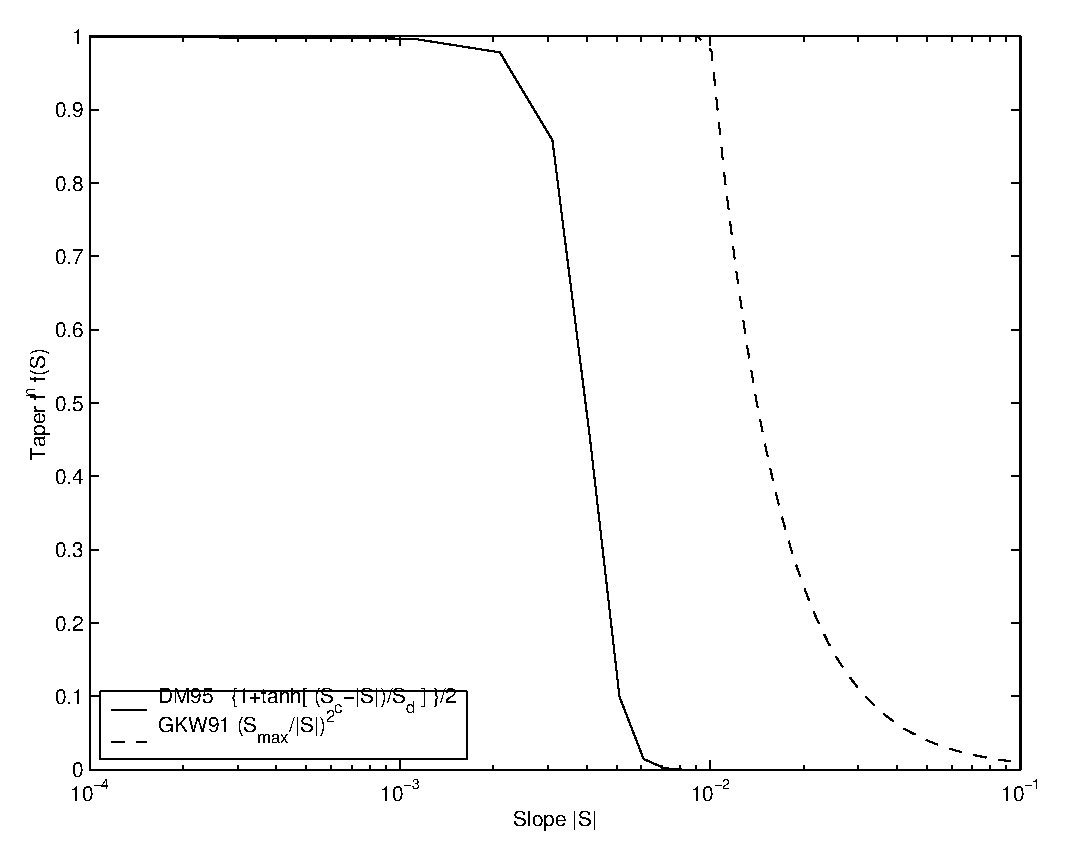
\includegraphics{part6/tapers.eps}}
\end{center}
\caption{Taper functions used in GKW99 and DM95.}
\label{fig:tapers}
\end{figure}

\begin{figure}
\begin{center}
\resizebox{5.0in}{3.0in}{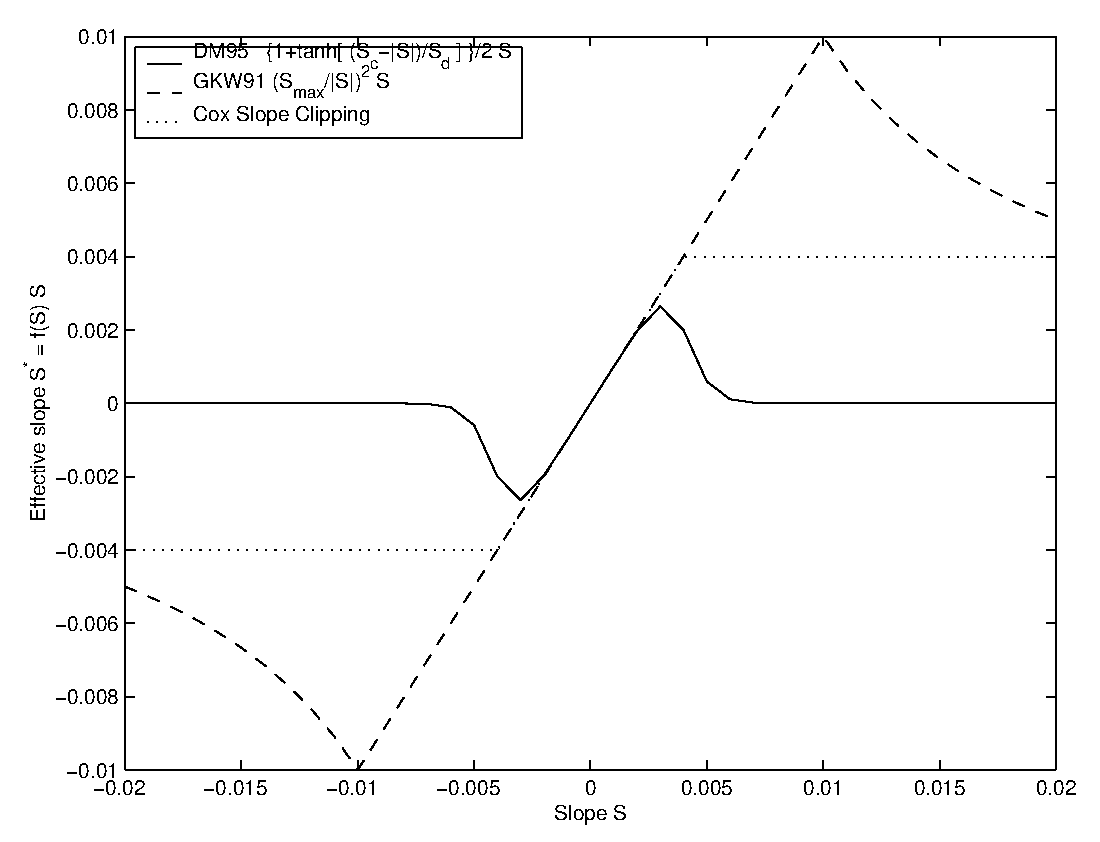
\includegraphics{part6/effective_slopes.eps}}
\end{center}
\caption{Effective slope as a function of ``true'' slope using Cox
slope clipping, GKW91 limiting and DM95 limiting.}
\label{fig:effective_slopes}
\end{figure}


\subsubsection{Slope clipping}

Deep convection sites and the mixed layer are indicated by
homogenized, unstable or nearly unstable stratification. The slopes in
such regions can be either infinite, very large with a sign reversal
or simply very large. From a numerical point of view, large slopes
lead to large variations in the tensor elements (implying large bolus
flow) and can be numerically unstable. This was first recognized by
Cox, 1987, who implemented ``slope clipping'' in the isopycnal mixing
tensor. Here, the slope magnitude is simply restricted by an upper
limit:
\begin{eqnarray}
|\nabla \sigma| & = & \sqrt{ \sigma_x^2 + \sigma_y^2 } \\
S_{lim} & = & - \frac{|\nabla \sigma|}{ S_{max} }
\;\;\;\;\;\;\;\; \mbox{where $S_{max}$ is a parameter} \\
\sigma_z^\star & = & \min( \sigma_z , S_{lim} ) \\
{[s_x,s_y]} & = & - \frac{ [\sigma_x,\sigma_y] }{\sigma_z^\star}
\end{eqnarray}
Notice that this algorithm assumes stable stratification through the
``min'' function. In the case where the fluid is well stratified ($\sigma_z < S_{lim}$) then the slopes evaluate to:
\begin{equation}
{[s_x,s_y]} = - \frac{ [\sigma_x,\sigma_y] }{\sigma_z}
\end{equation}
while in the limited regions ($\sigma_z > S_{lim}$) the slopes become:
\begin{equation}
{[s_x,s_y]} = \frac{ [\sigma_x,\sigma_y] }{|\nabla \sigma|/S_{max}}
\end{equation}
so that the slope magnitude is limited $\sqrt{s_x^2 + s_y^2} =
S_{max}$.

The slope clipping scheme is activated in the model by setting {\bf
GM\_tap\-er\_scheme = 'clipping'} in {\em data.gmredi}.

Even using slope clipping, it is normally the case that the vertical
diffusion term (with coefficient $\kappa_\rho{\bf K}_{33} =
\kappa_\rho S_{max}^2$) is large and must be time-stepped using an
implicit procedure (see section on discretisation and code later).
Fig. \ref{fig-mixedlayer} shows the mixed layer depth resulting from
a) using the GM scheme with clipping and b) no GM scheme (horizontal
diffusion). The classic result of dramatically reduced mixed layers is
evident. Indeed, the deep convection sites to just one or two points
each and are much shallower than we might prefer. This, it turns out,
is due to the over zealous re-stratification due to the bolus transport
parameterization. Limiting the slopes also breaks the adiabatic nature
of the GM/Redi parameterization, re-introducing diabatic fluxes in
regions where the limiting is in effect.

\subsubsection{Tapering: Gerdes, Koberle and Willebrand, Clim. Dyn. 1991}

The tapering scheme used in Gerdes et al., 1999, (\cite{gkw:99})
addressed two issues with the clipping method: the introduction of
large vertical fluxes in addition to convective adjustment fluxes is
avoided by tapering the GM/Redi slopes back to zero in
low-stratification regions; the adjustment of slopes is replaced by a
tapering of the entire GM/Redi tensor. This means the direction of
fluxes is unaffected as the amplitude is scaled.

The scheme inserts a tapering function, $f_1(S)$, in front of the
GM/Redi tensor:
\begin{equation}
f_1(S) = \min \left[ 1, \left( \frac{S_{max}}{|S|}\right)^2 \right]
\end{equation}
where $S_{max}$ is the maximum slope you want allowed. Where the
slopes, $|S|<S_{max}$ then $f_1(S) = 1$ and the tensor is un-tapered
but where $|S| \ge S_{max}$ then $f_1(S)$ scales down the tensor so
that the effective vertical diffusivity term $\kappa f_1(S) |S|^2 =
\kappa S_{max}^2$.

The GKW tapering scheme is activated in the model by setting {\bf
GM\_tap\-er\_scheme = 'gkw91'} in {\em data.gmredi}.

\subsection{Tapering: Danabasoglu and McWilliams, J. Clim. 1995}

The tapering scheme used by Danabasoglu and McWilliams, 1995,
\cite{dm:95}, followed a similar procedure but used a different
tapering function, $f_1(S)$:
\begin{equation}
f_1(S) = \frac{1}{2} \left( 1+\tanh \left[ \frac{S_c - |S|}{S_d} \right] \right)
\end{equation}
where $S_c = 0.004$ is a cut-off slope and $S_d=0.001$ is a scale over
which the slopes are smoothly tapered. Functionally, the operates in
the same way as the GKW91 scheme but has a substantially lower
cut-off, turning off the GM/Redi SGS parameterization for weaker
slopes.

The DM tapering scheme is activated in the model by setting {\bf
GM\_tap\-er\_scheme = 'dm95'} in {\em data.gmredi}.

\subsection{Tapering: Large, Danabasoglu and Doney, JPO 1997}

The tapering used in Large et al., 1997, \cite{ldd:97}, is based on the
DM95 tapering scheme, but also tapers the scheme with an additional
function of height, $f_2(z)$, so that the GM/Redi SGS fluxes are
reduced near the surface:
\begin{equation}
f_2(S) = \frac{1}{2} \left( 1 + \sin(\pi \frac{z}{D} - \pi/2)\right)
\end{equation}
where $D = L_\rho |S|$ is a depth-scale and $L_\rho=c/f$ with
$c=2$~m~s$^{-1}$.  This tapering with height was introduced to fix
some spurious interaction with the mixed-layer KPP parameterization.

The LDD tapering scheme is activated in the model by setting {\bf
GM\_tap\-er\_scheme = 'ldd97'} in {\em data.gmredi}.




\begin{figure}
\begin{center}
%\includegraphics{mixedlayer-cox.eps}
%\includegraphics{mixedlayer-diff.eps}
Figure missing.
\end{center}
\caption{Mixed layer depth using GM parameterization with a) Cox slope
clipping and for comparison b) using horizontal constant diffusion.}
\label{fig-mixedlayer}
\end{figure}






\newpage
\subsection{KPP Package: Ocean vertical mixing -- 
the nonlocal K-profile parameterization scheme}

\label{sec:pkg:kpp}
\begin{rawhtml}
<!-- CMIREDIR:package_kpp: -->
\end{rawhtml}


\newpage
% \documentclass[12pt]{article}
% \usepackage{amssymb}

%%%%%%%%%%%%%%%%%%%%%%%%%%%%%%%%%%%%%%%%%%%
%%  \usepackage{graphics}


% \oddsidemargin -4mm \evensidemargin 0mm
% \textwidth 165mm
% \textheight 230mm
% \topmargin -2mm \headsep -2mm
% \renewcommand{\baselinestretch}{1.5}
% \begin{document}


\def\deg{$^o$}
%%%--------------------------------------%%%
\section{THSICE: The Thermodynamic Sea Ice Package}
\label{sec:pkg:thsice}
\begin{rawhtml}
<!-- CMIREDIR:package_thsice: -->
\end{rawhtml}

{\bf Important note:}
This document has been written by Stephanie Dutkiewicz
and describes an earlier implementation of the sea-ice package.
This needs to be updated to reflect the recent changes (JMC).

\noindent
This thermodynamic ice model is based on the 3-layer model by Winton (2000).
and the energy-conserving LANL CICE model (Bitz and Lipscomb, 1999).
The model considers two equally thick ice layers; the upper layer has
a variable specific heat resulting from brine pockets,
the lower layer has a fixed heat capacity. A zero heat capacity snow
layer lies above the ice. Heat fluxes at the top and bottom
surfaces are used to calculate the change in ice and snow layer
thickness. Grid cells of the ocean model are 
either fully covered in ice or are open water. There is
a provision to parametrize ice fraction (and leads) in this package.
Modifications are discussed in small font following the
subroutine descriptions.

%%%%%%%%%%%%%%%%%%%%%%%%%%%%%%%%%%%%%%%%%%%%%%%%%%%%%%%%%%%%%%

\vspace{1cm}

\noindent
The ice model is called from {\it thermodynamics.F}, subroutine
{\it ice\_forcing.F} is called in place of {\it external\_forcing\_surf.F}.

%%%%%%%%%%%%%%%%%%%%%%%%%%%%%%%%%%%%%%%%%%%%%%%%%%%%%%%%%%%%%%

\vspace{1cm}
\noindent
{\bf \underline{subroutine ICE\_FORCING}}

\noindent
In {\it ice\_forcing.F}, we calculate the freezing potential of the
ocean model surface layer of water:
\[
  {\bf frzmlt} = (T_f - SST) \frac{c_{sw} \rho_{sw} \Delta z}{\Delta t}
\]
where $c_{sw}$ is seawater heat capacity, 
$\rho_{sw}$ is the seawater density, $\Delta z$
is the ocean model upper layer thickness and $\Delta t$ is the model (tracer)
timestep. The freezing temperature, $T_f=\mu S$ is a function of the
salinity.


1) Provided there is no ice present and {\bf frzmlt} is less than 0,
   the surface tendencies of wind, heat and freshwater are calculated
   as usual (ie. as in {\it external\_forcing\_surf.F}).

2) If there is ice present in the grid cell
   we call the main ice model routine {\it ice\_therm.F} (see below).
   Output from this routine gives net heat and freshwater flux 
   affecting the top of the ocean.

Subroutine {\it ice\_forcing.F} uses these values to find the 
sea surface tendencies
in grid cells. When there is ice present,  
the surface stress tendencies are
set to zero; the ice model is purely thermodynamic and the
effect of ice motion on the sea-surface is not examined.

Relaxation of surface $T$ and $S$ is only allowed equatorward
of {\bf relaxlat} (see {\bf DATA.ICE below}), and no relaxation is
allowed under the ice at any latitude.

\noindent
{\tiny (Note that there is provision for allowing grid cells to have both
open water and seaice; if {\bf compact} is between  0 and 1)}

%%%%%%%%%%%%%%%%%%%%%%%%%%%%%%%%%%%%%%%%%%%%%%%%%%%%%%%%%%%%%%
\vspace{1cm}
\noindent
{\bf {\underline{ subroutine ICE\_FREEZE}}}

This routine is called from {\it thermodynamics.F}
after the new temperature calculation, {\it calc\_gt.F}, 
but before {\it calc\_gs.F}.
In {\it ice\_freeze.F}, any ocean upper layer grid cell
with no ice cover, but with temperature below freezing,
$T_f=\mu S$ has ice initialized.
We calculate {\bf frzmlt} from all the grid cells in
the water column that have a temperature less than
freezing. In this routine, any water below the surface
that is below freezing is set to $T_f$.
A call to
{\it ice\_start.F} is made if {\bf frzmlt} $>0$, 
and salinity tendancy is updated for brine release.

\noindent
{\tiny (There is a provision for fractional ice:
In the case where the grid cell has less ice coverage than
{\bf icemaskmax} we allow {\it ice\_start.F} to be called).}

%%%%%%%%%%%%%%%%%%%%%%%%%%%%%%%%%%%%%%%%%%%%%%%%%%%%%%%%%%%%%%%%%%%

\vspace{1cm}
\noindent
{\bf {\underline{ subroutine ICE\_START}}}

\noindent
The energy available from freezing
the sea surface is brought into this routine as {\bf esurp}.
The enthalpy of the 2 layers of any new ice is calculated as:
\begin{eqnarray}
q_1 & = & -c_{i}*T_f + L_i \nonumber \\
q_2 & = & -c_{f}T_{mlt}+ c_{i}(T_{mlt}-T{f}) + L_i(1-\frac{T_{mlt}}{T_f} 
\nonumber \\
\end{eqnarray}
where  $c_f$ is specific heat of liquid fresh water, $c_i$ is the
specific heat of fresh ice, $L_i$ is latent heat of freezing, 
$\rho_i$ is density of ice and
$T_{mlt}$ is melting temperature of ice with salinity of 1.
The height of a new layer of ice is
\[
  h_{i new} = \frac{{\bf esurp} \Delta t}{qi_{0av}}
\]
where $qi_{0av}=-\frac{\rho_i}{2} (q_1+q_2)$.

The surface skin temperature $T_s$ and ice temperatures
$T_1$, $T_2$ and the sea surface temperature are set at $T_f$.

\noindent
{\tiny ( There is provision for fractional ice:
new ice is formed over open water; the first freezing in the cell
must have a height of {\bf himin0}; this determines the ice
fraction {\bf compact}. If there is already ice in the grid cell,
the new ice must have the same height and the new ice fraction
is 
\[
i_f=(1-\hat{i_f}) \frac{h_{i new}}{h_i}
\]
where $\hat{i_f}$ is ice fraction from previous timestep
and $h_i$ is current ice height. Snow is redistributed 
over the new ice fraction. The ice fraction is
not allowed to become larger than {\bf iceMaskmax} and
if the ice height is above {\bf hihig} then freezing energy
comes from the full grid cell,  ice growth does not occur
under orginal ice due to freezing water.
}
%%%%%%%%%%%%%%%%%%%%%%%%%%%%%%%%%%%%%%%%%%%%%%%%%%%%%%%%%%%%%%%%%%%

\vspace{1cm}
\noindent
{\bf {\underline{subroutine ICE\_THERM}}}

\noindent
The main subroutine of this package is {\it ice\_therm.F} where the
ice temperatures are calculated and the changes in ice and snow
thicknesses are determined. Output provides the net heat and fresh 
water fluxes that force the top layer of the ocean model.

If the current ice height is less than {\bf himin} then
the ice layer is set to zero and the ocean model upper layer temperature
is allowed to drop lower than its freezing temperature; and atmospheric
fluxes are allowed to effect the grid cell.
If the ice height is greater than  {\bf himin} we proceed with
the ice model calculation.

We follow the procedure
of Winton (1999) -- see equations 3 to 21 -- to calculate
the surface and internal ice temperatures. 
The surface temperature is found from the balance of the
flux at the surface $F_s$, the shortwave heat flux absorbed by the ice, 
{\bf fswint}, and
the upward conduction of heat through the snow and/or ice, $F_u$.
We linearize $F_s$ about the surface temperature, $\hat{T_s}$, 
at the previous timestep (where \mbox{}$\hat{ }$ indicates the value at
the  previous timestep):
\[
F_s (T_s) = F_s(\hat{T_s}) + \frac{\partial F_s(\hat{T_s)}}{\partial T_s}
(T_s-\hat{T_s})
\]
where, 
\[
F_s  =  F_{sensible}+F_{latent}+F_{longwave}^{down}+F_{longwave}^{up}+ (1-
\alpha) F_{shortwave}
\]
and
\[
 \frac{d F_s}{dT} = \frac{d F_{sensible}}{dT} + \frac{d F_{latent}}{dT}
+\frac{d F_{longwave}^{up}}{dT}.
\]
$F_s$ and $\frac{d F_s}{dT}$ are currently calculated from the {\bf BULKF} 
package described separately, but could also be provided by an atmospheric
model. The surface albedo is calculated from the ice height and/or 
surface temperature (see below, {\it srf\_albedo.F}) and the 
shortwave flux absorbed in the ice is
\[
{\bf fswint} = (1-e^{\kappa_i h_i})(1-\alpha) F_{shortwave}
\]
where $\kappa_i$ is bulk extinction coefficient.

The conductive flux to the surface is
\[
F_u=K_{1/2}(T_1-T_s)
\]
where $K_{1/2}$ is the effective conductive coupling of the snow-ice
layer between the surface and the mid-point of the upper layer of ice
$
K_{1/2}=\frac{4 K_i K_s}{K_s h_i + 4 K_i h_s}
$.
$K_i$ and $K_s$ are constant thermal conductivities of seaice and snow.

From the above equations we can develop a system of equations to
find the skin surface temperature, $T_s$ and the two ice layer
temperatures (see Winton, 1999, for details). We solve these
equations iteratively until the change in $T_s$ is small.
When the surface temperature is greater then
the melting temperature of the surface, the temperatures are
recalculated setting $T_s$ to 0.  The enthalpy
of the ice layers are calculated in order to keep track of the energy in the
ice model. Enthalpy is defined, here, as the energy required to melt a
unit mass of seaice with temperature $T$.
For the upper layer (1) with brine pockets  and
the lower fresh layer (2):
\begin{eqnarray}
q_1 & = & - c_f T_f + c_i (T_f-T)+ L_{i}(1-\frac{T_f}{T})
\nonumber \\
q_2 & = & -c_i T+L_i \nonumber
\end{eqnarray}
where $c_f$ is specific heat of liquid fresh water, $c_i$ is the
specific heat of fresh ice, and $L_i$ is latent heat of melting fresh ice.



From the new ice temperatures, we can calculate
the energy flux at the surface available for melting (if $T_s$=0)
and the energy at the ocean-ice interface for either melting or freezing.
\begin{eqnarray}
E_{top} &  =  & (F_s- K_{1/2}(T_s-T_1) ) \Delta t
\nonumber \\
E_{bot} &= & (\frac{4K_i(T_2-T_f)}{h_i}-F_b) \Delta t
\nonumber
\end{eqnarray}
where $F_b$ is the heat flux at the ice bottom due to the sea surface
temperature variations from freezing.
If $T_{sst}$ is above freezing, $F_b=c_{sw} \rho_{sw} 
\gamma (T_{sst}-T_f)u^{*}$, $\gamma$ is the heat transfer coefficient
and $u^{*}=QQ$ is frictional velocity between ice 
and water. If $T_{sst}$ is below freezing,
$F_b=(T_f - T_{sst})c_f \rho_f \Delta z /\Delta t$ and set $T_{sst}$
to $T_f$. We also
include the energy from lower layers that drop below freezing,
and set those layers to $T_f$.

If $E_{top}>0$ we melt snow from the surface, if all the snow is melted
and there is energy left, we melt the ice. If the ice is all gone
and there is still energy left, we apply the left over energy to 
heating the ocean model upper layer (See Winton, 1999, equations 27-29).
Similarly if $E_{bot}>0$ we melt ice from the bottom. If all the ice
is melted, the snow is melted (with energy from the ocean model upper layer
if necessary). If $E_{bot}<0$ we grow ice at the bottom
\[
\Delta h_i = \frac{-E_{bot}}{(q_{bot} \rho_i)}
\]
where $q_{bot}=-c_{i} T_f + L_i$ is the enthalpy of the new ice,
The enthalpy of the second ice layer, $q_2$ needs to be modified:
\[
q_2 = \frac{ \hat{h_i}/2 \hat{q_2} + \Delta h_i q_{bot} }
        {\hat{h_i}/{2}+\Delta h_i}
\]

If there is a ice layer and the overlying air temperature is
below 0$^o$C then any precipitation, $P$ joins the snow layer:
\[
\Delta h_s  = -P \frac{\rho_f}{\rho_s} \Delta t, 
\]
$\rho_f$ and $\rho_s$ are the fresh water and snow densities.
Any evaporation, similarly, removes snow or ice from the surface.
We also calculate the snow age here, in case it is needed for
the surface albedo calculation (see {\it srf\_albedo.F} below).

For practical reasons we limit the ice growth to {\bf hilim}
and snow is limited to {\bf hslim}. We converts any
ice and/or snow above these limits back to water, maintaining the salt
balance. Note however, that heat is not conserved in this
conversion; sea surface temperatures below the ice are not
recalculated.

If the snow/ice interface is below the waterline, snow is converted
to ice (see Winton, 1999, equations 35 and 36). The subroutine
{\it new\_layers\_winton.F}, described below, repartitions the ice into
equal thickness layers while conserving energy.

The subroutine {\it ice\_therm.F} now calculates the heat and fresh
water fluxes affecting the ocean model surface layer. The heat flux:
\[
q_{net}= {\bf fswocn} - F_{b} - \frac{{\bf esurp}}{\Delta t}
\]
is composed of the shortwave flux that has passed through the
ice layer and is absorbed by the water, {\bf fswocn}$=QQ$,
the ocean flux to the ice $F_b$,
and the surplus energy left over from the melting, {\bf esurp}.
The fresh water flux is determined from the amount of
fresh water and salt in the ice/snow system before and after the
timestep.

\noindent
{\tiny (There is a provision for fractional ice:
If ice height is above {\bf hihig} then all energy from freezing at
sea surface is used only in the open water aparts of the cell (ie.
$F_b$ will only have the conduction term).
The melt energy is partitioned by {\bf frac\_energy} between melting
ice height and ice extent. However, once ice height drops below
{\bf himon0} then all energy melts ice extent.}

%%%%%%%%%%%%%%%%%%%%%%%%%%%%%%%%%%%%%%%%%%%%%%%%%%%%%%%%%%%%%%%
\vspace{1cm}

\noindent
{\bf {\underline{subroutine SFC\_ALBEDO} } }

\noindent
The routine {\it ice\_therm.F} calls this routine to determine
the surface albedo. There are two calculations provided here:

\noindent
{\bf 1)} from LANL CICE model
\[ \alpha = f_s \alpha_s + (1-f_s) (\alpha_{i_{min}}
         + (\alpha_{i_{max}}- \alpha_{i_{min}}) (1-e^{-h_i/h_{\alpha}}))
\]
where $f_s$ is 1 if there is snow, 0 if not; the snow albedo, 
$\alpha_s$ has two values
depending on whether $T_s<0$ or not; $\alpha_{i_{min}}$ and 
$\alpha_{i_{max}}$ are ice albedos for thin melting ice, and
thick bare ice respectively, and $h_{\alpha}$ is a scale
height.

\noindent
{\bf 2)} From GISS model (Hansen et al 1983)
\[
 \alpha = \alpha_i e^{-h_s/h_a} + \alpha_s (1-e^{-h_s/h_a})
\]
where $\alpha_i$ is a constant albedo for bare ice, $h_a$
is a scale height and $\alpha_s$ is a variable snow albedo.
\[
\alpha_s = \alpha_1 + \alpha_2 e^{-\lambda_a a_s}
\]
where $\alpha_1$ is a constant, $\alpha_2$ depends on $T_s$,
$a_s$ is the snow age, and $\lambda_a$ is a scale frequency.
The snow age is calculated in {\it ice\_therm.F} and is given
in equation 41 in Hansen et al (1983).

%%%%%%%%%%%%%%%%%%%%%%%%%%%%%%%%%%%%%%%%%%%%%%%%%%%%%%%%%%%%%%%

\vspace{1cm}

\noindent
{\bf {\underline{subroutine NEW\_LAYERS\_WINTON}}}

\noindent
The subroutine
{\it new\_layers\_winton.F} repartitions the ice into
equal thickness layers while conserving energy. We pass
to this subroutine, the ice layer enthalpies after
melting/growth and the new height of the ice layers.
The ending layer height should be half the sum of the
new ice heights from {\it ice\_therm.F}. The enthalpies
of the ice layers are adjusted accordingly to maintain
total energy in the ice model. If layer 2 height is
greater than layer 1 height then layer 2 gives ice to
layer 1 and:
\[
q_1=f_1 \hat{q_1} + (1-f1) \hat{q_2}
\]
where $f_1$ is the fraction of the new to old upper layer heights.
$T_1$ will therefore also have changed.
Similarly for when ice layer height 2 is less than
layer 1 height, except here we need to to be careful
that the new $T_2$ does not fall below the melting temperature.

%%%%%%%%%%%%%%%%%%%%%%%%%%%%%%%%%%%%%%%%%%%%%%%%%%%%%%%%%%%%%%%

\vspace{1cm}

\noindent
{\bf {\underline{Initializing subroutines}}}

\noindent
{\it ice\_init.F}:
Set ice variables to zero, or reads in pickup information
from {\bf pickup.ic} (which was written out in {\it checkpoint.F})

\noindent
{\it ice\_readparms.F}:
Reads {\bf data.ice}

%%%%%%%%%%%%%%%%%%%%%%%%%%%%%%%%%%%%%%%%%%%%%%%%%%%%%%%%%%%%%%%

\vspace{1cm}

\noindent
{\bf {\underline{Diagnostic subroutines}}}

\noindent
{\it ice\_ave.F}:
Keeps track of means of the ice variables

\noindent
{\it ice\_diags.F}:
Finds averages and writes out diagnostics

%%%%%%%%%%%%%%%%%%%%%%%%%%%%%%%%%%%%%%%%%%%%%%%%%%%%%%%%%%%%%%%%
\vspace{1cm}

\noindent
{\bf {\underline{Common Blocks}}}

\noindent
{\it ICE.h}: Ice Varibles, also 
{\bf relaxlat} and {\bf startIceModel}

\noindent
{\it ICE\_DIAGS.h}: matrices for diagnostics: averages of fields
from {\it ice\_diags.F}

\noindent
{\it BULKF\_ICE\_CONSTANTS.h} (in {\bf BULKF} package): 
all the parameters need by the ice model

%%%%%%%%%%%%%%%%%%%%%%%%%%%%%%%%%%%%%%%%%%%%%%%%%%%%%%%%%%%%%%%%%%
\vspace{1cm}

\noindent
{\bf {\underline{Input file DATA.ICE}}}

\noindent
Here we need to set {\bf StartIceModel}: which is 1 if the
model starts from no ice; and 0 if there is a pickup file
with the ice matrices ({\bf pickup.ic}) which is read
in {\it ice\_init.F} and written out in {\it checkpoint.F}.
The parameter {\bf relaxlat} defines the latitude poleward
of which there is no relaxing of surface $T$ or $S$ to
observations. This avoids the relaxation forcing the ice
model at these high latitudes.

\noindent
({\tiny Note: {\bf hicemin} is set to 0 here. If the
provision for allowing grid cells to have both
open water and seaice is ever implemented, this would
be greater than 0})

%%%%%%%%%%%%%%%%%%%%%%%%%%%%%%%%%%%%%%%%%%%%%%%%%%%%%%%%%%%%
\vspace{1cm}

\noindent
{\bf {\underline{Important Notes}}}

\noindent
{\bf 1)} heat fluxes have different signs in the ocean and ice
models.

\noindent
{\bf 2)} {\bf StartIceModel} must be changed in {\bf data.ice}:
1 (if starting from no ice), 0 (if using pickup.ic file).

%%%%%%%%%%%%%%%%%%%%%%%%%%%%%%%%%%%%%%%%%%%%%%%%%%%%%%%%%%%%%%

\vspace{1cm}

\noindent 
{\bf {\underline{References}}}

\noindent
Bitz, C.M. and W.H. Lipscombe, 1999: An Energy-Conserving
Thermodynamic Model of Sea Ice.
{\it Journal of Geophysical Research}, 104, 15,669 -- 15,677.

\vspace{.2cm}

\noindent
Hansen, J., G. Russell, D. Rind, P. Stone, A. Lacis, S. Lebedeff,
R. Ruedy and L.Travis, 1983: Efficient Three-Dimensional
Global Models for Climate Studies: Models I and II.
{\it Monthly Weather Review}, 111, 609 -- 662.

\vspace{.2cm}

\noindent
Hunke, E.C and W.H. Lipscomb, circa 2001: CICE: the Los Alamos
Sea Ice Model Documentation and Software User's Manual.
LACC-98-16v.2.\\
(note: this documentation is no longer available as CICE has progressed
to a very different version 3)


\vspace{.2cm}

\noindent
Winton, M, 2000: A reformulated Three-layer Sea Ice Model.
{\it Journal of Atmospheric and Ocean Technology}, 17, 525 -- 531.



%%%%%%%%%%%%%%%%%%%%%%%%%%%%%%%%%%%%%%%%%%%
% \end{document}


\newpage
% \documentclass[12pt]{article}
% \usepackage{amssymb}
% 
% \usepackage{graphics}
% 
% 
% \oddsidemargin -4mm \evensidemargin 0mm
% \textwidth 165mm
% \textheight 230mm
% \topmargin -2mm \headsep -2mm
% \renewcommand{\baselinestretch}{1.5}
% \begin{document}
% 

%%%--------------------------------------%%%
\def\deg{$^o$}
\section{BULK\_FORCE: Bulk Formula Package}
\label{sec:pkg:bulk_formula}
\begin{rawhtml}
<!-- CMIREDIR:package_bulk_formula: -->
\end{rawhtml}

author: Stephanie Dutkiewicz\\

\noindent
Instead of forcing the model with heat and fresh water flux data,
this package calculates these fluxes using the changing sea surface
temperature. We need to read in some atmospheric data:
{\bf air temperature, air humidity, down shortwave radiation,
     down longwave radiation, precipitation, wind speed}.
The current setup also reads in {\bf wind stress}, but this
can be changed so that the stresses are calculated from the
wind speed.

The current setup requires that there is the thermodynamic-seaice package
({\it pkg/thsice}, also refered below as seaice)
is also used. It would be useful though to have it also
setup to run with some very simple parametrization of the sea ice.

%%%%%%%%%%%%%%%%%%%%%%%%%%%%%%%%%%%%%%%%%%%%%%%%%%%%%%%%%%%%%%

\vspace{1cm}

\noindent
The heat and fresh water fluxes are calculated in {\it bulkf\_forcing.F}
called from {\it forward\_step.F}. These fluxes are used over open water,
fluxes over seaice are recalculated in the sea-ice package.
Before the call to {\it bulkf\_forcing.F} we call 
{\it bulkf\_fields\_load.F} to find the current atmospheric conditions.
The only other changes to the model code come from the initializing
and writing diagnostics of these fluxes.

%%%%%%%%%%%%%%%%%%%%%%%%%%%%%%%%%%%%%%%%%%%%%%%%%%%%%%%%%%%%%%
\vspace{1cm}
\noindent
{\bf \underline{subroutine BULKF\_FIELDS\_LOAD}}

\noindent
Here we find the atmospheric data needed for the bulk formula
calculations. These are read in at periodic intervals and
values are interpolated to the current time. The data file names
come from {\bf data.blk}. The values that can be read in are:
air temperature, air humidity, precipitation, 
down solar radiation, down long
wave radiation, zonal and meridional wind speeds, total wind
speed, net heat flux, net freshwater forcing, cloud cover,
snow fall, zonal and meridional wind stresses, and SST and SSS
used for relaxation terms.
Not all these files are necessary or used. For instance cloud
cover and snow fall are not used in the current bulk formula
calculation. If total wind speed is not supplied, wind speed
is calculate from the zonal and meridional components. If
wind stresses are not read in, then the stresses are calculated
from the wind speed. Net heat flux and net freshwater can be
read in and used over open ocean instead of the bulk formula
calculations (but over seaice the bulkf formula is always
used). This is "hardwired" into {\it bulkf\_forcing} and
the "ch" in the variable names suggests that this is "cheating".
SST and SSS need to be read in if there is any relaxation used.


%%%%%%%%%%%%%%%%%%%%%%%%%%%%%%%%%%%%%%%%%%%%%%%%%%%%%%%%%%%%%%


\vspace{1cm}
\noindent
{\bf \underline{subroutine BULKF\_FORCING}}

\noindent
In {\it bulkf\_forcing.F}, we calculate  heat and fresh water
fluxes (and wind stress, if necessary) for each grid cell.
First we determine if the grid cell is open water or seaice
and this information is carried by {\bf iceornot}. There is
a provision here for a different designation if there is
snow cover (but currently this does not make any difference).
We then call {\it bulkf\_formula\_lanl.F} which provides
values for: up long wave radiation, latent and sensible heat
fluxes, the derivative of these three with respect to surface
temperature, wind stress, evaporation. 
Net long wave radiation is calculated from the combination
of the down long wave read in and the up long wave calculated.

We then find the albedo of the surface - with a call to
{\it sfc\_albedo} if there is sea-ice (see the seaice package
for information on the subroutine). If the grid cell is open
ocean the albedo is set as 0.1. Note that this is a parameter
that can be used to tune the results. The net short wave
radiation is then the down shortwave radiation minus the 
amount reflected.

If the wind stress needed to be calculated in {\it bulkf\_formula\_lanl.F},
it was calculated to grid cell center points, so in {\it bulkf\_forcing.F}
we regrid to {\bf u} and {\bf v} points. We let the model know
if it has read in stresses or calculated stresses by the switch
{\bf readwindstress} which is can be set in data.blk, and defaults
to {\bf .TRUE.}.

We then calculate {\bf Qnet} and {\bf EmPmR} that will be used
as the fluxes over the open ocean. There is a provision for
using runoff. If we are "cheating" and using observed fluxes 
over the open ocean, then there is a provision here to
use read in {\bf Qnet} and {\bf EmPmR}.

The final call is to calculate averages of the terms found
in this subroutine.

%%%%%%%%%%%%%%%%%%%%%%%%%%%%%%%%%%%%%%%%%%%%%%%%%%%%%%%%%%%%%%
\vspace{1cm}
\noindent
{\bf {\underline{ subroutine BULKF\_FORMULA\_LANL}}}

\noindent
This is the main program of the package where the
heat fluxes and freshwater fluxes over ice and
open water are calculated. Note that this subroutine
is also called from the seaice package during the
iterations to find the ice surface temperature.

Latent heat ($L$) used in this subroutine 
depends on the state of the surface: vaporization for
open water, fusion and vaporization for ice surfaces.
Air temperature is converted from Celsius to Kelvin.
If there is no wind speed ($u_s$) given, then the wind speed
is calculated from the zonal and meridional components.

We calculate the virtual temperature:
\[
T_o = T_{air} (1+\gamma q_{air})
\]
where $T_{air}$ is the air temperature at $h_T$, $q_{air}$ is
humidity at $h_q$ and $\gamma$ is a constant.

The saturated vapor pressure is calculate (QQ ref):
\[
q_{sat} = \frac{a}{p_o} e^{L (b-\frac{c}{T_{srf}})}
\]
where $a,b,c$ are constants, $T_{srf}$ is surface temperature
and $p_o$ is the surface pressure.

The two values crucial for the bulk formula calculations are
the difference between air at sea surface and sea surface temperature:
\[
\Delta T = T_{air} - T_{srf} +\alpha h_T
\]
where $\alpha$ is adiabatic lapse rate and $h_T$ is the  height
where the air temperature was taken; and the difference
between the air humidity and the saturated humidity
\[
\Delta q = q_{air} - q_{sat}.
\]

We then calculate the turbulent exchange coefficients
following Bryan et al (1996) and the numerical scheme
of Hunke and Lipscombe (1998). 
We estimate initial values for the exchange coefficients, $c_u$,
$c_T$ and $c_q$ as
\[
\frac{\kappa}{ln(z_{ref}/z_{rou})}
\]
where $\kappa$ is the Von Karman constant, $z_{ref}$ is a
reference height and $z_{rou}$ is a roughness length scale
which could be a function of type of surface, but is here set
as a constant. Turbulent scales are:
\begin{eqnarray}
u^* & = & c_u u_s \nonumber\\
T^* & = & c_T \Delta T \nonumber\\
q^* & = & c_q \Delta q \nonumber
\end{eqnarray}

We find the "integrated flux profile" for momentum and stability
if there are stable QQ conditions ($\Upsilon>0$) :
\[
\psi_m = \psi_s = -5 \Upsilon
\]
and for unstable QQ conditions ($\Upsilon<0$):
\begin{eqnarray}
\psi_m & = & 2 ln(0.5(1+\chi)) + ln(0.5(1+\chi^2)) - 2 \tan^{-1} \chi + \pi/2
\nonumber \\
\psi_s & = & 2 ln(0.5(1+\chi^2)) \nonumber
\end{eqnarray}
where
\[
\Upsilon = \frac{\kappa g z_{ref}}{u^{*2}} (\frac{T^*}{T_o} + 
\frac{q^*}{1/\gamma + q_a})
\]
and $\chi=(1-16\Upsilon)^{1/2}$.

The coefficients are updated through 5 iterations as:
\begin{eqnarray}
c_u & = & \frac {\hat{c_u}}{1+\hat{c_u}(\lambda - \psi_m)/\kappa} \nonumber \\
c_T & = & \frac {\hat{c_T}}{1+\hat{c_T}(\lambda - \psi_s)/\kappa} \nonumber \\
c_q & = & c'_T
\end{eqnarray}
where $\lambda =ln(h_T/z_{ref})$.

We can then find the bulk formula heat fluxes:

\vspace{.2cm}
\noindent
Sensible heat flux:
\[
Q_s=\rho_{air} c_{p_{air}} u_s c_u c_T \Delta T
\]

\vspace{.2cm}
\noindent
Latent heat flux:
\[
Q_l=\rho_{air} L u_s c_u c_q \Delta q
\]

\vspace{.2cm}
\noindent
Up long wave radiation
\[
Q_{lw}^{up}=\epsilon \sigma T_{srf}^4
\]
where $\epsilon$ is emissivity (which can be different for
open ocean, ice and snow), $\sigma$ is Stefan-Boltzman constant.

We calculate the derivatives of the three above functions
with respect to surface temperature
\begin{eqnarray}
\frac{dQ_s}{d_T} & = & \rho_{air} c_{p_{air}} u_s c_u c_T \nonumber \\
\frac{dQ_l}{d_T} & = & \frac{\rho_{air} L^2 u_s c_u c_q c}{T_{srf}^2} \nonumber \\
\frac{dQ_{]lw}^{up}}{d_T} & = &  4 \epsilon \sigma t_{srf}^3 \nonumber
\end{eqnarray}

And total derivative $\frac{dQ_o}{dT}= \frac{dQ_s}{dT} +
\frac{dQ_l}{dT} + \frac{dQ_{lw}^{up}}{dT}$.




If we do not read in the wind stress, it is calculated here.

%%%%%%%%%%%%%%%%%%%%%%%%%%%%%%%%%%%%%%%%%%%%%%%%%%%%%%%%%%%%%%%

\vspace{1cm}

\noindent
{\bf {\underline{Initializing subroutines}}}

\noindent
{\it bulkf\_init.F}:
Set bulkf variables to zero.

\noindent
{\it bulkf\_readparms.F}:
Reads {\bf data.blk}

%%%%%%%%%%%%%%%%%%%%%%%%%%%%%%%%%%%%%%%%%%%%%%%%%%%%%%%%%%%%%%%

\vspace{1cm}

\noindent
{\bf {\underline{Diagnostic subroutines}}}

\noindent
{\it bulkf\_ave.F}:
Keeps track of means of the bulkf variables

\noindent
{\it bulkf\_diags.F}:
Finds averages and writes out diagnostics

%%%%%%%%%%%%%%%%%%%%%%%%%%%%%%%%%%%%%%%%%%%%%%%%%%%%%%%%%%%%%%%%
\vspace{1cm}

\noindent
{\bf {\underline{Common Blocks}}}

\noindent
{\it BULKF.h}: BULKF Variables,  data file names, and logicals
{\bf readwindstress} and {\bf readsurface}

\noindent
{\it BULKF\_DIAGS.h}: matrices for diagnostics: averages of fields
from {\it bulkf\_diags.F}

\noindent
{\it BULKF\_ICE\_CONSTANTS.h}: 
all the parameters need by the ice model and in the bulkf formula
calculations.

%%%%%%%%%%%%%%%%%%%%%%%%%%%%%%%%%%%%%%%%%%%%%%%%%%%%%%%%%%%%%%%%%%
\vspace{1cm}

\noindent
{\bf {\underline{Input file DATA.ICE}}}

\noindent
We read in the file names of atmospheric data used in
the  bulk formula calculations. Here we can also set
the logicals: {\bf readwindstress} if we read in the
wind stress rather than calculate it from the wind
speed; and {\bf readsurface} to read in the surface
temperature and salinity if these will be used as
part of a relaxing term.

%%%%%%%%%%%%%%%%%%%%%%%%%%%%%%%%%%%%%%%%%%%%%%%%%%%%%%%%%%%%
\vspace{1cm}

\noindent
{\bf {\underline{Important Notes}}}

\noindent
{\bf 1)} heat fluxes have different signs in the ocean and ice
models.

\noindent
{\bf 2)} {\bf StartIceModel} must be changed in {\bf data.ice}:
1 (if starting from no ice), 0 (if using pickup.ic file).

%%%%%%%%%%%%%%%%%%%%%%%%%%%%%%%%%%%%%%%%%%%%%%%%%%%%%%%%%%%%%%

\vspace{1cm}

\noindent 
{\bf {\underline{References}}}


\vspace{.2cm}

\noindent
Bryan F.O., B.G Kauffman, W.G. Large, P.R. Gent, 1996:
The NCAR CSM flux coupler. Technical note TN-425+STR,
NCAR.

\vspace{.2cm}

\noindent
Hunke, E.C and W.H. Lipscomb, circa 2001: CICE: the Los Alamos
Sea Ice Model Documentation and Software User's Manual.
LACC-98-16v.2.\\
(note: this documentation is no longer available as CICE has progressed
to a very different version 3)





%%%%%%%%%%%%%%%%%%%%%%%%%%%%%%%%%%%%%%%%%%%
% \end{document}


\newpage
\section{Land package}

This package provides a simple land model
based on Rong Zhang [e-mail:roz@gfdl.noaa.gov] 2 layers model
(see documentation below).

It is primarily implemented for AIM (\_v23) atmospheric physics
but could be adapted to work with a different atmospheric physics.
Two subroutines ({\it aim\_aim2land.F} {\it aim\_land2aim.F}
in {\it pkg/aim\_v23}) are used as interface with AIM physics. 

Number of layers is a parameter ({\it land\_nLev} in {\it LAND\_SIZE.h})
and can be changed. 

%---------------------------------------------------------------------

% \documentclass[12pt,thmsa]{article}

% \begin{document}

\begin{center}
{\bf Note on Land Model}\\
date: June 1999\\
author: Rong Zhang\\
\end{center}

% \baselineskip19pt

This is a simple 2-layer land model. The top layer depth $z1=0.1m$, the
second layer depth $z2=4m$.

Let $T_{g1},T_{g2}$ be the temperature of each layer, $W_{1,}W_{2}$ be the
soil moisture of each layer. The field capacity $f_{1,}$ $f_{2}$ are the
maximum water amount in each layer, so $W_{i}$ is the ratio of available
water to field capacity. $f_{i}=\gamma z_{i},\gamma =0.24$ is the field
capapcity per meter soil$,$ so $f_{1}=0.024m,$ $f_{2}=0.96m.$

The land temperature is determined by total surface downward heat flux $F,$

\begin{equation}
z_{1}C_{1}\frac{dT_{g1}}{dt}=F-\lambda \frac{T_{g1}-T_{g2}}{(z_{1}+z_{2})/2}
\end{equation}

\begin{center}
\begin{equation}
z_{2}C_{2}\frac{dT_{g2}}{dt}=\lambda \frac{T_{g1}-T_{g2}}{(z_{1}+z_{2})/2}
\end{equation}
\end{center}

here $C_{1},C_{2}$ are the heat capacity of each layer , $\lambda $ is the
thermal conductivity, $\lambda =0.42Wm^{-1}K^{-1}.$

\begin{center}
\bigskip 
\begin{equation}
C_{1}=C_{w}W_{1}\gamma +C_{s}
\end{equation}

\begin{equation}
C_{2}=C_{w}W_{2}\gamma +C_{s}
\end{equation}
\end{center}

$C_{w},C_{s}$ are the heat capacity of water and dry soil respectively. $%
C_{w}=4.2\times 10^{6}Jm^{-3}K^{-1},C_{s}=1.13\times 10^{6}Jm^{-3}K^{-1}.$

\bigskip

The soil moisture is determined by precipitation $P(m/s)$,surface
evaporation $E(m/s)$ and runoff $R(m/s).$

\begin{equation}
\frac{dW_{1}}{dt}=\frac{P-E-R}{f_{1}}+\frac{W_{2}-W_{1}}{\tau }
\end{equation}

$\tau =2$ $days$ is the time constant for diffusion of moisture between
layers.

\begin{equation}
\frac{dW_{2}}{dt}=\frac{f_{1}}{f_{2}}\frac{W_{1}-W_{2}}{\tau }
\end{equation}

In the code, $R=0$ gives better result, $W_{1},W_{2}$ are set to be within
[0, 1]. If $W_{1}$ is greater than 1, then let $\delta W_{1}=W_{1}-1,W_{1}=1$
and $W_{2}=W_{2}+p\delta W_{1}\frac{f_{1}}{f_{2}}$, i.e. the runoff of top
layer is put into second layer. $p=0.5$ is the fraction of top layer runoff
that is put into second layer.

The time step is 1 hour, it takes several years to reach equalibrium offline.

\begin{center}
\bigskip
\end{center}

\textbf{References}

Hansen J. et al. Efficient three-dimensional global models for climate
studies: models I and II. \emph{Monthly Weather Review}, vol.111, no.4, pp.
609-62, 1983

% \end{document}


\newpage
\section{Coupling interface for Atmospheric Intermediate code}
\label{sec:aim_compon_interf}
\subsection{Key subroutines, parameters and files}
\label{sec:pkg:aim_compon_interf:implementation_synopsis}
\subsection{Package Reference}


\newpage
\section{Coupler for mapping between AIM and ocean }
\label{sec:pkg:aim_ocn_coupler}
\begin{rawhtml}
<!-- CMIREDIR:package_aim_ocn_coupler: -->
\end{rawhtml}

\subsection{Key subroutines, parameters and files}
\label{sec:pkg:aim_ocn_coupler:implementation_synopsis}


\newpage
\subsection{Toolkit for building couplers}
\label{sec:component_communications}
\label{sec:pkg:component_communications}
\begin{rawhtml}
<!-- CMIREDIR:package_component_communications: -->
\end{rawhtml}

\subsubsection{Key subroutines, parameters and files}
\label{sec:pkg:component_communications:implementation_synopsis}

\subsubsection{Experiments and tutorials that use component\_communications}
\label{sec:pkg:component_communications:experiments}

\begin{itemize}
\item{Global coupled ocean atmosphere experiment in cpl\_aim+ocean verification directory. }
\end{itemize}


\newpage
% $Header: /u/gcmpack/manual/s_phys_pkgs/Attic/mnc.tex,v 1.12 2004/10/12 18:16:03 edhill Exp $
% $Name:  $

\section{NetCDF I/O Integration: MNC}
\label{sec:pkg:mnc}
\begin{rawhtml}
<!-- CMIREDIR:package_mnc: -->
\end{rawhtml}

The \texttt{mnc} package is a set of convenience routines written to
expedite the process of creating, appending, and reading NetCDF files.
NetCDF is an increasingly popular self-describing file format
\cite{rew:97} intended primarily for scientific data sets.  An
extensive collection of NetCDF reference papers, user guides,
software, FAQs, and other information can be obtained from UCAR's web
site at:
\begin{rawhtml} <A href="http://www.unidata.ucar.edu/packages/netcdf/"> \end{rawhtml}
\begin{verbatim}
http://www.unidata.ucar.edu/packages/netcdf/
\end{verbatim}
\begin{rawhtml} </A> \end{rawhtml}


\subsection{Using MNC}

\subsubsection{MNC Configuration and Inputs}

As with all MITgcm packages, MNC can be turned on/off at compile time
using the \texttt{packages.conf} file or the genmake2
\texttt{-enable=mnc} or \texttt{-disable=mnc} switches.

For run-time configuration, most of the MNC--related model parameters
are contained within a Fortran namelist file called \texttt{data.mnc}.
If this file does not exist, then the MNC package will interpret that
as an indication that it is not to be used.  If the \texttt{data.mnc}
file does exist, then it may contain the following parameters:

\begin{center}
  {\footnotesize
    \begin{tabular}[htb]{|l|c|l|l|}\hline
      \textbf{Name}  &  \textbf{T}  &  
      \textbf{Default}  &  \textbf{Description}  \\\hline
      &  &  &  \\
      \texttt{useMNC}  &  L  & \texttt{.FALSE.}  &  
      \textbf{overall MNC ON/OFF switch}  \\
      \texttt{mnc\_echo\_gvtypes}  &  L  & \texttt{.FALSE.}  &  
      echo pre-defined ``types'' (debugging)   \\
      \texttt{mnc\_use\_outdir}  &  L  & \texttt{.FALSE.}  &  
      create a directory for output  \\
      \texttt{mnc\_outdir\_str}  &  S  & \texttt{'mnc\_'}  &  
      output directory name \\
      \texttt{mnc\_outdir\_date}  &  L  & \texttt{.FALSE.}  &  
      embed date in the output dir name  \\
      \texttt{pickup\_write\_mnc}  &  L  & \texttt{.FALSE.}  &  
      use MNC to write (create) pickup files  \\
      \texttt{pickup\_read\_mnc}  &  L  & \texttt{.FALSE.}  &  
      use MNC to read pickup files  \\
      \texttt{mnc\_use\_indir}  &  L  & \texttt{.FALSE.}  &  
      use a directory (path) for input  \\
      \texttt{mnc\_indir\_str}  &  S  & \texttt{''}  &  
      input directory (or path) name  \\
      \texttt{snapshot\_mnc}  &  L  & \texttt{.FALSE.}  &  
      write \texttt{snapshot} (instantaneous) w/MNC  \\
      \texttt{monitor\_mnc}  &  L  & \texttt{.FALSE.}  &  
      write \texttt{monitor} w/MNC  \\
      \texttt{timeave\_mnc}  &  L  & \texttt{.FALSE.}  &  
      write \texttt{timeave} w/MNC  \\
      \texttt{autodiff\_mnc}  &  L  & \texttt{.FALSE.}  &  
      write \texttt{autodiff} w/MNC  \\\hline
    \end{tabular}
  }
\end{center}

Additional MNC--related parameters are contained within the main
\texttt{data} namelist file and in some of the namelist files for
individual packages.  These options are:
\begin{center}
  {\footnotesize
    \begin{tabular}[htb]{|l|c|l|l|}\hline
      \textbf{Name}  &  \textbf{T}  &  
      \textbf{Default}  &  \textbf{Description}  \\\hline
      \multicolumn{4}{|c|}{\ }  \\
      \multicolumn{4}{|c|}{Main namelist file: 
        ``\textbf{data}''}  \\\hline
      \texttt{snapshot\_ioinc}  &  L  & \texttt{.FALSE.}  &  
      write \texttt{snapshot} ``inclusively''  \\
      \texttt{timeave\_ioinc}  &  L  & \texttt{.FALSE.}  &  
      write \texttt{timeave} ``inclusively''  \\
      \texttt{monitor\_ioinc}  &  L  & \texttt{.FALSE.}  &  
      write \texttt{monitor} ``inclusively''  \\
      \texttt{the\_run\_name}  &  C  & ``name...''  &  
      name is included in all MNC output  \\\hline
      \multicolumn{4}{|c|}{\ }  \\
      \multicolumn{4}{|c|}{Diagnostics namelist file: 
        ``\textbf{data.diagnostics}''}  \\\hline
      \texttt{diag\_mnc}  &  L  & \texttt{.FALSE.}  &  
      write \texttt{diagnostics} w/MNC  \\
      \texttt{diag\_ioinc}  &  L  & \texttt{.FALSE.}  &  
      write \texttt{diagnostics} ``inclusively''  \\\hline
    \end{tabular}
  }
\end{center}

By default, turning on MNC for a particular output type will result in
turning off all the corresponding (usually, default) MDSIO or STDOUT
output mechanisms.  In other words, output defaults to being an
exclusive selection.  To enable multiple kinds of simultaneous output,
flags of the form \texttt{NAME\_ioinc} have been created where
\texttt{NAME} corresponds to the various MNC output flags.  When a
\texttt{NAME\_ioinc} flag is set to \texttt{.TRUE.}, then multiple
simultaneous forms of output are allowed for the \texttt{NAME} output
mechanism.  The intent of this design is that typical users will only
want one kind of output while people debugging the code (particularly
the I/O routines) may want simultaneous types of output.

This ``inclusive'' versus ``exclusive'' design is easily applied in
cases where three or more kinds of output may be generated.  Thus, it
can be readily extended to additional new output types (eg. HDF5).

Input types are always exclusive.

\subsubsection{MNC Output}

While NetCDF files are supposed to be ``self-describing'', it is
helpful to note the following:

\begin{itemize}
\item The constraints placed upon the ``unlimited'' (or ``record'')
  dimension inherent with NetCDF v3.x make it very inefficient to put
  variables written at potentially different intervals within the same
  file.  For this reason, MNC output is split into a few file ``base
  names'' which try to reflect the nature of their content.
  
\item All MNC output is currently done in a ``tile-per-file'' fashion
  since most NetCDF v3.x implementions cannot write safely within MPI
  or multi-threaded environments.  This tiling is done in a global
  fashion and the tile numbers are appended to the base names
  described above.  Some scripts to ``assemble'' output are available
  (\texttt{MITgcm/utils/matlab}).  More general manipulations can be
  accomplished with the
  \begin{rawhtml}
    <A href="http://nco.sourceforge.net"> 
  \end{rawhtml} 
\begin{verbatim}
NetCDF Operators (or ``NCO'') at http://nco.sourceforge.net
\end{verbatim}
  \begin{rawhtml} </A> \end{rawhtml}
  which is a very powerful and convenient set of tools for working
  with all NetCDF files.
  
\item MNC does not (yet) provide a mechanism for reading information
  from a single ``global'' file as can be done with the MDSIO
  package.

\end{itemize}


\subsection{MNC Internals}

The \texttt{mnc} package is a two-level convenience library (or
``wrapper'') for most of the NetCDF Fortran API.  Its purpose is to
streamline the user interface to NetCDF by maintaining internal
relations (look-up tables) keyed with strings (or names) and entities
such as NetCDF files, variables, and attributes.

The two levels of the \texttt{mnc} package are:
\begin{description}

\item[Upper level] \ 
  
  The upper level contains information about two kinds of
  associations:
  \begin{description}
  \item[grid type] is lookup table indexed with a grid type name.
    Each grid type name is associated with a number of dimensions, the
    dimension sizes (one of which may be unlimited), and starting and
    ending index arrays.  The intent is to store all the necessary
    size and shape information for the Fortran arrays containing
    MITgcm--style ``tile'' variables (that is, a central region
    surrounded by a variably-sized ``halo'' or exchange region as
    shown in Figures \ref{fig:communication_primitives} and
    \ref{fig:tiling-strategy}).
  
  \item[variable type] is a lookup table indexed by a variable type
    name.  For each name, the table contains a reference to a grid
    type for the variable and the names and values of various
    attributes.
  \end{description}
  
  Within the upper level, these associations are not permanently tied
  to any particular NetCDF file.  This allows the information to be
  re-used over multiple file reads and writes.

\item[Lower level] \ 
  
  In the lower (or internal) level, associations are stored for NetCDF
  files and many of the entities that they contain including
  dimensions, variables, and global attributes.  All associations are
  on a per-file basis.  Thus, each entity is tied to a unique NetCDF
  file and will be created or destroyed when files are, respectively,
  opened or closed.

\end{description}


\subsubsection{MNC Grid--Types and Variable--Types}

As a convenience for users, the MNC package includes numerous routines
to aid in the writing of data to NetCDF format.  Probably the biggest
convenience is the use of pre-defined ``grid types'' and ``variable
types''.  These ``types'' are simply look-up tables that store
dimensions, indicies, attributes, and other information that can all
be retrieved using a single character string.

The ``grid types'' are a way of mapping variables within MITgcm to
NetCDF arrays.  Within MITgcm, most spatial variables are defined
using two-- or three--dimensional arrays with ``overlap'' regions (see
Figures \ref{fig:communication_primitives}, a possible vertical index,
and \ref{fig:tiling-strategy}) and tile indicies such as the following
``U'' velocity:
\begin{verbatim}
      _RL  uVel (1-OLx:sNx+OLx,1-OLy:sNy+OLy,Nr,nSx,nSy)
\end{verbatim}
as defined in \filelink{model/inc/DYNVARS.h}{model-inc-DYNVARS.h}

The grid type is a character string that encodes the presence and
types associated with the four possible dimensions.  The character
string follows the format
\begin{center}
  \texttt{H0\_H1\_H2\_\_V\_\_T}
\end{center}
where the terms \textit{H0}, \textit{H1}, \textit{H2}, \textit{V},
\textit{T} can be almost any combination of the following:
\begin{center}
  \begin{tabular}[h]{|ccc|c|c|}\hline
    \multicolumn{3}{|c|}{Horizontal} & Vertical & Time \\
    \textbf{H0}: location & \textbf{H1}: dimensions & \textbf{H2}: halo 
          & \textbf{V}: location & \textbf{T}: level  \\\hline
    \texttt{-} & xy & Hn & \texttt{-} & \texttt{-} \\
    U  &  x  &  Hy  &  i  &  t  \\
    V  &  y  &      &  c  &     \\
    Cen  &   &      &     &     \\
    Cor  &   &      &     &     \\\hline
  \end{tabular}
\end{center}
A example list of all pre-defined combinations is contained in the
file
\begin{center}
  \texttt{pkg/mnc/pre-defined\_grids.txt}.
\end{center}

The variable type is an association between a variable type name and the
following items:
\begin{center}
  \begin{tabular}[h]{|l|l|}\hline
    \textbf{Item}  & \textbf{Purpose}  \\\hline
    grid type  &  defines the in-memory arrangement  \\
    \texttt{bi,bj} dimensions  &  tiling indices, if present  \\\hline
  \end{tabular}
\end{center}
and is used by the \texttt{mnc\_cw\_*\_[R|W]} subroutines for reading
and writing variables.


\subsubsection{Using MNC: Examples}

Writing variables to NetCDF files can be accomplished in as few as two
function calls.  The first function call defines a variable type,
associates it with a name (character string), and provides additional
information about the indicies for the tile (\texttt{bi},\texttt{bj})
dimensions.  The second function call will write the data at, if
necessary, the current time level within the model.

Examples of the initialization calls can be found in the file 
\filelink{model/src/ini\_mnc\_io.F}{model-src-ini_mnc_io.F}
where these function calls:
{\footnotesize
\begin{verbatim}
C     Create MNC definitions for DYNVARS.h variables
      CALL MNC_CW_ADD_VNAME('iter', '-_-_--__-__t', 0,0, myThid)
      CALL MNC_CW_ADD_VATTR_TEXT('iter',1,
     &     'long_name','iteration_count', myThid)

      CALL MNC_CW_ADD_VNAME('model_time', '-_-_--__-__t', 0,0, myThid)
      CALL MNC_CW_ADD_VATTR_TEXT('model_time',1,
     &     'long_name','Model Time', myThid)
      CALL MNC_CW_ADD_VATTR_TEXT('model_time',1,'units','s', myThid)

      CALL MNC_CW_ADD_VNAME('U', 'U_xy_Hn__C__t', 4,5, myThid)
      CALL MNC_CW_ADD_VATTR_TEXT('U',1,'units','m/s', myThid)
      CALL MNC_CW_ADD_VATTR_TEXT('U',1,
     &     'coordinates','XU YU RC iter', myThid)

      CALL MNC_CW_ADD_VNAME('T', 'Cen_xy_Hn__C__t', 4,5, myThid)
      CALL MNC_CW_ADD_VATTR_TEXT('T',1,'units','degC', myThid)
      CALL MNC_CW_ADD_VATTR_TEXT('T',1,'long_name',
     &     'potential_temperature', myThid)
      CALL MNC_CW_ADD_VATTR_TEXT('T',1,
     &     'coordinates','XC YC RC iter', myThid)
\end{verbatim}
}
{\noindent initialize four \texttt{VNAME}s and add one or more NetCDF
  attributes to each.}
    
The four variables defined above are subsequently written at specific
time steps within
\filelink{model/src/write\_state.F}{model-src-write_state.F}
using the function calls:
{\footnotesize
\begin{verbatim}
C       Write dynvars using the MNC package
        CALL MNC_CW_SET_UDIM('state', -1, myThid)
        CALL MNC_CW_I_W('I','state',0,0,'iter', myIter, myThid)
        CALL MNC_CW_SET_UDIM('state', 0, myThid)
        CALL MNC_CW_RL_W('D','state',0,0,'model_time',myTime, myThid)
        CALL MNC_CW_RL_W('D','state',0,0,'U', uVel, myThid)
        CALL MNC_CW_RL_W('D','state',0,0,'T', theta, myThid)
\end{verbatim}
}

While it is easiest to write variables within typical 2D and 3D fields
where all data is known at a given time, it is also possible to write
fields where only a portion (\textit{eg.} a ``slab'' or ``slice'') is
known at a given instant.  An example is provided within
\filelink{pkg/mom\_vecinv/mom\_vecinv.F}{pkg-mom_vecinv-mom_vecinv.F}
where an offset vector is used: {\footnotesize
\begin{verbatim}
       IF (useMNC .AND. snapshot_mnc) THEN
         CALL MNC_CW_RL_W_OFFSET('D','mom_vi',bi,bj, 'fV', uCf,
   &          offsets, myThid)
         CALL MNC_CW_RL_W_OFFSET('D','mom_vi',bi,bj, 'fU', vCf,
   &          offsets, myThid)
       ENDIF
\end{verbatim}
}
to write a 3D field one depth slice at a time.

Each element in the offset vector corresponds (in order) to the
dimensions of the ``full'' (or virtual) array and specifies which are
known at the time of the call.  A zero within the offset array means
that all values along that dimension are available while a positive
integer means that only values along that index of the dimension are
available.  In all cases, the matrix passed is assumed to start (that
is, have an in-memory structure) coinciding with the start of the
specified slice.  Thus, using this offset array mechanism, a slice
can be written along any single dimension or combinations of
dimensions.


% $Header: /u/gcmpack/manual/s_outp_pkgs/text/mdsio.tex,v 1.6 2006/04/04 20:51:09 molod Exp $
% $Name:  $


\section{Fortran Native I/O: MDSIO and RW}
\label{sec:mdsio_and_rw}


\subsection{MDSIO}
\label{sec:pkg:mdsio}
\begin{rawhtml}
<!-- CMIREDIR:package_mdsio: -->
\end{rawhtml}
\label{sec:pkg:rw}

\subsubsection{Introduction}
The \texttt{mdsio} package contains a group of Fortran routines
intended as a general interface for reading and writing direct-access
(``binary'') Fortran files.  The \texttt{mdsio} routines are used by
the \texttt{rw} package.

The \texttt{mdsio} package is currently the primary method for MITgcm
I/O, but it is not being actively extended or enhanced.  Instead, the
\texttt{mnc} netCDF package (see Section \ref{sec:pkg:mnc}) is
expected to gain all of the current \texttt{mdsio} functionality and,
eventually, replace it.  For the short term, every effort has been
made to allow \texttt{mnc} and \texttt{mdsio} to peacefully co-exist.
In may cases, the model can read one format and write to the other.
This side-by-side functionality can be used to, for instance, help
convert pickup files or other data sets between the two formats.


\subsubsection{Using MDSIO}
The \texttt{mdsio} package is geared toward the reading and writing of
floating point (Fortran \texttt{REAL*4} or \texttt{REAL*8}) arrays.
It assumes that the in-memory layout of all arrays follows the per-tile
MITgcm convention
\begin{verbatim}
C     Example of a "2D" array
      _RL anArray(1-OLx:sNx+OLx,1-OLy:sNy+OLy,nSx,nSy)

C     Example of a "3D" array
      _RL anArray(1-OLx:sNx+OLx,1-OLy:sNy+OLy,1:Nr,nSx,nSy)
\end{verbatim}
where the first two dimensions are spatial or ``horizontal'' indicies
that include a ``halo'' or exchange region (please see
Chapters \ref{chap:sarch} and \ref{sec:exch2} which describe domain
decomposition), and the remaining indicies (\texttt{Nr},\texttt{nSx},
and \texttt{nSx}) are often present but not required.

In order to write output, the \texttt{mdsio} package is called with a
function such as:
\begin{verbatim}
      CALL MDSWRITEFIELD(fn,prec,lgf,typ,Nr,arr,irec,myIter,myThid)
\end{verbatim}
where:
\begin{quote}
  \begin{description}
  \item[\texttt{fn}] is a \texttt{CHARACTER} string containing a file
    ``base'' name which will then be used to create file names that
    contain tile and/or model iteration indicies
  \item[\texttt{prec}] is an integer that contains one of two globally
    defined values (\texttt{precFloat64} or \texttt{precFloat32})
  \item[\texttt{lgf}] is a \texttt{LOGICAL} that typically contains
    the globally defined \texttt{globalFile} option which specifies
    the creation of globally (spatially) concatenated files
  \item[\texttt{typ}] is a \texttt{CHARACTER} string that specifies
    the type of the variable being written (\texttt{'RL'} or
    \texttt{'RS'})
  \item[\texttt{Nr}] is an integer that specifies the number of
    vertical levels within the variable being written
  \item[\texttt{arr}] is the variable (array) to be written
  \item[\texttt{irec}] is the starting record within the output file
    that will contain the array
  \item[\texttt{myIter,myThid}] are integers containing, respectively,
    the current model iteration count and the unique thread ID for the
    current context of execution
  \end{description}  
\end{quote}
As one can see from the above (generic) example, enough information is
made available (through both the argument list and through common blocks)
for the \texttt{mdsio} package to perform the following tasks:
\begin{enumerate}
\item open either a per-tile file such as:
  \begin{center}
    \texttt{uVel.0000302400.003.001.data}
  \end{center}
  or a ``global'' file such as
  \begin{center}
    \texttt{uVel.0000302400.data}
  \end{center}
\item byte-swap (as necessary) the input array and write its contents
  (minus any halo information) to the binary file -- or to the correct
  location within the binary file if the globalfile option is used, and 
\item create an ASCII--text metadata file (same name as the binary but
  with a \texttt{.meta} extension) describing the binary file contents
  (often, for later use with the MatLAB \texttt{rdmds()} utility).
\end{enumerate}

Reading output with \texttt{mdsio} is very similar to writing it.  A
typical function call is
\begin{verbatim}
      CALL MDSREADFIELD(fn,prec,typ,Nr,arr,irec,myThid)
\end{verbatim}
where variables are exactly the same as the \texttt{MDSWRITEFIELD}
example provided above.  It is important to note that the \texttt{lgf}
argument is missing from the \texttt{MDSREADFIELD} function.  By
default, \texttt{mdsio} will first try to read from an appropriately
named global file and, failing that, will try to read from a per-tile
file.


\subsubsection{Important Considerations}
When using \texttt{mdsio}, one should be aware of the following
package features and limitations:
\begin{description}
\item[Byte-swapping] is, for the most part, gracefully handled.  All
  files intended for reading/writing by \texttt{mdsio} should contain
  big-endian (sometimes called ``network byte order'') data.  By
  handling byte-swapping within the model, MITgcm output is more
  easily ported between different machines, architectures, compilers,
  etc.  Byteswapping can be turned on/off at compile time within
  \texttt{mdsio} using the \texttt{\_BYTESWAPIO} CPP macro which is
  usually set within a \texttt{genmake2} options file or
  ``\texttt{optfile}'' which are located in
\begin{verbatim}
      MITgcm/tools/build_options
\end{verbatim}
  Additionally, some compilers may have byte-swap options that are
  speedier or more convenient to use.

\item[Types] are currently limited to single-- or double--precision
  floating point values.  These values can be converted, on-the-fly,
  from one to the other so that any combination of either single-- or
  double--precision variables can be read from or written to files
  containing either single-- or double--precision data.

\item[Array sizes] are limited.  The \texttt{mdsio} package is very
  much geared towards the reading/writing of per-tile (that is,
  domain-decomposed and halo-ed) arrays.  Data that cannot be made to
  ``fit'' within these assumed sizes can be challenging to read or
  write with \texttt{mdsio}.

\item[Tiling] or domain decomposition is automatically handled by
  \texttt{mdsio} for logically rectangular grid topologies
  (\textit{eg.} lat-lon grids) and ``standard'' cubesphere topologies.
  More complicated topologies will probably not be supported.  The
  \texttt{mdsio} package can, without any coding changes, read and
  write to/from files that were run on the same global grid but with
  different tiling (grid decomposition) schemes.  For example,
  \texttt{mdsio} can use and/or create identical input/output files
  for a ``C32'' cube when the model is run with either 6, 12, or 24
  tiles (corresponding to 1, 2 or 4 tiles per cubesphere face).
  Currently, this is one of the primary advantages that the
  \texttt{mdsio} package has over \texttt{mnc}.

\item[Single-CPU I/O] can be specified with the flag
\begin{verbatim}
       useSingleCpuIO = .TRUE.,
\end{verbatim}
  in the \texttt{PARM01} namelist within the main \texttt{data} file.
  Single--CPU I/O mode is appropriate for computers (\textit{eg.} some
  SGI systems) where it can either speed overall I/O or solve problems
  where the operating system or file systems cannot correctly handle
  multiple threads or MPI processes simultaneously writing to the same
  file.

\item[Meta-data] is written by MITgcm on a per-file basis using a
  second file with a \texttt{.meta} extension as described above.
  MITgcm itself does not read the \texttt{*.meta} files, they are
  there primarly for convenience during post-processing.  One should
  be careful not to delete the meta-data files when using MatLAB
  post-processing scripts such as \texttt{rdmds()} since it relies
  upon them.

\item[Numerous files] can be written by \texttt{mdsio} due to its
  typically per-time-step and per-variable orientation.  The creation of
  both a binary (\texttt{*.data}) and ASCII text meta-data
  (\texttt{*.meta}) file for each output type step tends to exacerbate
  the problem.  Some (mostly, older) operating systems do not
  gracefully handle large numbers (\textit{eg.} many thousands) of
  files within one directory.  So care should be taken to split output
  into smaller groups using subdirectories.

\item[Overwriting] is the \textbf{default behavior} for
  \texttt{mdsio}.  If a model tries to write to a file name that
  already exists, the older file \textbf{will be deleted}.  For this
  reason, MITgcm users should be careful to move output that that wish
  to keep into, for instance, subdirectories before performing
  subsequent runs that may over--lap in time or otherwise produce
  files with identical names (\textit{eg.} Monte-Carlo simulations).

\item[No ``halo'' information] is written or read by \texttt{mdsio}.
  Along the horizontal dimensions, all variables are written in an
  \texttt{sNx}--by--\texttt{sNy} fashion.  So, although variables
  (arrays) may be defined at different locations on Arakawa grids [U
  (right/left horizontal edges), V (top/bottom horizontal edges), M
  (mass or cell center), or Z (vorticity or cell corner) points], they
  are all written using only interior (\texttt{1:sNx} and
  \texttt{1:sNy}) values.  For quantities defined at U, V, and M
  points, writing \texttt{1:sNx} and \texttt{1:sNy} for every tile is
  sufficient to ensure that all values are written globally for some
  grids (eg. cubesphere, re-entrant channels, and doubly-periodic
  rectangular regions).  For Z points, failing to write values at the
  \texttt{sNx+1} and \texttt{sNy+1} locations means that, for some
  tile topologies, not all values are written.  For instance, with a
  cubesphere topology at least two corner values are ``lost'' (fail to
  be written for any tile) if the \texttt{sNx+1} and \texttt{sNy+1}
  values are ignored.  To fix this problem, the \texttt{mnc} package
  writes the \texttt{sNx+1} and \texttt{sNy+1} grid values for the U,
  V, and Z locations.  Also, the \texttt{mnc} package is capable of
  reading and/or writing entire halo regions and more complicated
  array shapes which can be helpful when debugging--features that
  do not exist within \texttt{mdsio}.
\end{description}


\subsection{RW Basic binary I/O utilities}
\label{sec:pkg:rw}
\begin{rawhtml}
<!-- CMIREDIR:package_rw: -->
\end{rawhtml}

The {\tt rw} package provides a very rudimentary binary I/O capability
for quickly writing {\it single record} direct-access Fortran binary files.
It is primarily used for writing diagnostic output.

\subsubsection{Introduction}
Package {\tt rw} is an interface to the more general {\tt mdsio} package.
The {\tt rw} package can be used to write or read direct-access Fortran
binary files for two-dimensional XY and three-dimensional XYZ arrays.
The arrays are assumed to have been declared according to the standard
MITgcm two-dimensional or three-dimensional floating point array type:
\begin{verbatim}
C     Example of declaring a standard two dimensional "long"
C     floating point type array (the _RL macro is usually
C     mapped to 64-bit floats in most configurations)
      _RL anArray(1-OLx:sNx+OLx,1-OLy:sNy+OLy,nSx,nSy)
\end{verbatim}

Each call to an {\tt rw} read or write routine will read (or write) to
the first record of a file. To write direct access Fortran files with
multiple records use the package {\tt mdsio} (see section
\ref{sec:pkg:mdsio}).  To write self-describing files that contain
embedded information describing the variables being written and the
spatial and temporal locations of those variables use the package {\tt
  mnc} (see section \ref{sec:pkg:mnc}) which produces
\htlink{netCDF}{http://www.unidata.ucar.edu/packages/netcdf}
\cite{rew:97} based output.

%% \subsubsection{Key subroutines, parameters and files}
%% \label{sec:pkg:rw:implementation_synopsis}
%% The {\tt rw} package has



\newpage
\subsection{Monitor: Simulation state monitoring toolkit}
\label{sec:pkg:monitor}
\begin{rawhtml}
<!-- CMIREDIR:package_monitor: -->
\end{rawhtml}

\subsubsection{Key subroutines, parameters and files}
\label{sec:pkg:monitor:implementation_synopsis}


\newpage
% $Header: /u/gcmpack/manual/s_phys_pkgs/text/exch2.tex,v 1.27 2009/05/02 02:13:18 jmc Exp $
% $Name:  $

%%  * Introduction
%%    o what it does, citations (refs go into mitgcm_manual.bib, 
%%      preferably in alphabetic order)
%%    o Equations 
%%  * Key subroutines and parameters
%%  * Reference material (auto generated from Protex and structured comments)
%%    o automatically inserted at \section{Reference} 


\subsection{exch2: Extended Cubed Sphere \mbox{Topology}}
\label{sec:exch2}


\subsubsection{Introduction}

The \texttt{exch2} package extends the original cubed sphere topology
configuration to allow more flexible domain decomposition and
parallelization.  Cube faces (also called subdomains) may be divided
into any number of tiles that divide evenly into the grid point
dimensions of the subdomain.  Furthermore, the tiles can run on
separate processors individually or in groups, which provides for
manual compile-time load balancing across a relatively arbitrary
number of processors.

The exchange parameters are declared in
\filelink{pkg/exch2/W2\_EXCH2\_TOPOLOGY.h}{pkg-exch2-W2_EXCH2_TOPOLOGY.h}
and assigned in
\filelink{pkg/exch2/w2\_e2setup.F}{pkg-exch2-w2_e2setup.F}. The
validity of the cube topology depends on the \file{SIZE.h} file as
detailed below.  The default files provided in the release configure a
cubed sphere topology of six tiles, one per subdomain, each with
32$\times$32 grid points, with all tiles running on a single processor.  Both
files are generated by Matlab scripts in
\file{utils/exch2/matlab-topology-generator}; see Section
\ref{sec:topogen} \sectiontitle{Generating Topology Files for exch2}
for details on creating alternate topologies.  Pregenerated examples
of these files with alternate topologies are provided under
\file{utils/exch2/code-mods} along with the appropriate \file{SIZE.h}
file for single-processor execution.

\subsubsection{Invoking exch2}

To use exch2 with the cubed sphere, the following conditions must be
met:

\begin{itemize}
\item The exch2 package is included when \file{genmake2} is run.  The
  easiest way to do this is to add the line \code{exch2} to the
  \file{packages.conf} file -- see Section \ref{sect:buildingCode}
  \sectiontitle{Building the code} for general
  details.

\item An example of \file{W2\_EXCH2\_TOPOLOGY.h} and
  \file{w2\_e2setup.F} must reside in a directory containing files
  symbolically linked by the \file{genmake2} script.  The safest place
  to put these is the directory indicated in the \code{-mods=DIR}
  command line modifier (typically \file{../code}), or the build
  directory.  The default versions of these files reside in
  \file{pkg/exch2} and are linked automatically if no other versions
  exist elsewhere in the build path, but they should be left untouched
  to avoid breaking configurations other than the one you intend to
  modify.

\item Files containing grid parameters, named \file{tile00$n$.mitgrid}
  where $n$=\code{(1:6)} (one per subdomain), must be in the working
  directory when the MITgcm executable is run.  These files are
  provided in the example experiments for cubed sphere configurations
  with 32$\times$32 cube sides -- please contact MITgcm support if you
  want to generate files for other configurations.

\item As always when compiling MITgcm, the file \file{SIZE.h} must be
  placed where \file{genmake2} will find it.  In particular for exch2,
  the domain decomposition specified in \file{SIZE.h} must correspond
  with the particular configuration's topology specified in
  \file{W2\_EXCH2\_TOPOLOGY.h} and \file{w2\_e2setup.F}.  Domain
  decomposition issues particular to exch2 are addressed in Section
  \ref{sec:topogen} \sectiontitle{Generating Topology Files for exch2}
  and \ref{sec:exch2mpi} \sectiontitle{exch2, SIZE.h, and
    Multiprocessing}; a more general background on the subject
  relevant to MITgcm is presented in Section
  \ref{sect:specifying_a_decomposition}
  \sectiontitle{Specifying a decomposition}.
\end{itemize}

At the time of this writing the following examples use exch2 and may
be used for guidance:

\begin{verbatim}
verification/adjust_nlfs.cs-32x32x1
verification/adjustment.cs-32x32x1 
verification/aim.5l_cs
verification/global_ocean.cs32x15
verification/hs94.cs-32x32x5
\end{verbatim}




\subsubsection{Generating Topology Files for exch2}
\label{sec:topogen}

Alternate cubed sphere topologies may be created using the Matlab
scripts in \file{utils/exch2/matlab-topology-generator}. Running the
m-file
\filelink{driver.m}{utils-exch2-matlab-topology-generator_driver.m}
from the Matlab prompt (there are no parameters to pass) generates
exch2 topology files \file{W2\_EXCH2\_TOPOLOGY.h} and
\file{w2\_e2setup.F} in the working directory and displays a figure of
the topology via Matlab -- figures \ref{fig:6tile}, \ref{fig:18tile}, 
and \ref{fig:48tile} are examples of the generated diagrams.  The other 
m-files in the directory are
subroutines called from \file{driver.m} and should not be run ``bare'' except
for development purposes. \\

The parameters that determine the dimensions and topology of the
generated configuration are \code{nr}, \code{nb}, \code{ng},
\code{tnx} and \code{tny}, and all are assigned early in the script. \\

The first three determine the height and width of the subdomains and
hence the size of the overall domain.  Each one determines the number
of grid points, and therefore the resolution, along the subdomain
sides in a ``great circle'' around each the three spatial axes of the cube.  At the time
of this writing MITgcm requires these three parameters to be equal,
but they provide for future releases  to accomodate different
resolutions around the axes to allow subdomains with differing resolutions.\\

The parameters \code{tnx} and \code{tny} determine the width and height of
the tiles into which the subdomains are decomposed, and must evenly
divide the integer assigned to \code{nr}, \code{nb} and \code{ng}.
The result is a rectangular tiling of the subdomain.  Figure
\ref{fig:48tile} shows one possible topology for a twenty-four-tile
cube, and figure \ref{fig:6tile} shows one for six tiles. \\

\begin{figure}
\begin{center}
 \resizebox{6in}{!}{
% \includegraphics{part6/s24t_16x16.ps}
  \includegraphics{part6/adjust_cs.ps}
 }
\end{center} 

\caption{Plot of a cubed sphere topology with a 32$\times$192 domain
divided into six 32$\times$32 subdomains, each of which is divided
into eight tiles of width \code{tnx=16} and height \code{tny=8} for a 
total of forty-eight tiles. The colored borders of the subdomains 
represent the parameters \code{nr} (red), \code{ng} (green), and
\code{nb} (blue). 
This tiling is used in the example
verification/adjustment.cs-32x32x1/
with the option (blanklist.txt) to remove the land-only 4 tiles 
(11,12,13,14) which are filled in red on the plot.
} \label{fig:48tile}
\end{figure}

\begin{figure}
\begin{center}
 \resizebox{6in}{!}{
% \includegraphics{part6/s12t_16x32.ps}
  \includegraphics{part6/polarcap.ps}
 }
\end{center} 
\caption{Plot of a non-square cubed sphere topology with 
6 subdomains of different size (nr=90,ng=360,nb=90),
divided into one to four tiles each
 (\code{tnx=90, tny=90}), resulting in a total of 18 tiles.
} \label{fig:18tile}
\end{figure}

\begin{figure}
\begin{center}
 \resizebox{4in}{!}{
% \includegraphics{part6/s6t_32x32.ps}
  \includegraphics{part6/s6t_32x32.ps}
 }
\end{center} 
\caption{Plot of a cubed sphere topology with a 32$\times$192 domain
divided into six 32$\times$32 subdomains with one tile each
(\code{tnx=32, tny=32}).  This is the default configuration.
  }
\label{fig:6tile}
\end{figure}


Tiles can be selected from the topology to be omitted from being
allocated memory and processors.  This tuning is useful in ocean
modeling for omitting tiles that fall entirely on land.  The tiles
omitted are specified in the file
\filelink{blanklist.txt}{utils-exch2-matlab-topology-generator_blanklist.txt}
by their tile number in the topology, separated by a newline. \\




\subsubsection{exch2, SIZE.h, and Multiprocessing}
\label{sec:exch2mpi}

Once the topology configuration files are created, the Fortran
\code{PARAMETER}s in \file{SIZE.h} must be configured to match.
Section \ref{sect:specifying_a_decomposition} \sectiontitle{Specifying
  a decomposition} provides a general description of domain
decomposition within MITgcm and its relation to \file{SIZE.h}. The
current section specifies constraints that the exch2 package imposes
and describes how to enable parallel execution with MPI.

As in the general case, the parameters \varlink{sNx}{sNx} and
\varlink{sNy}{sNy} define the size of the individual tiles, and so
must be assigned the same respective values as \code{tnx} and
\code{tny} in \file{driver.m}.

The halo width parameters \varlink{OLx}{OLx} and \varlink{OLy}{OLy}
have no special bearing on exch2 and may be assigned as in the general
case. The same holds for \varlink{Nr}{Nr}, the number of vertical
levels in the model.

The parameters \varlink{nSx}{nSx}, \varlink{nSy}{nSy},
\varlink{nPx}{nPx}, and \varlink{nPy}{nPy} relate to the number of
tiles and how they are distributed on processors.  When using exch2,
the tiles are stored in the $x$ dimension, and so
\code{\varlink{nSy}{nSy}=1} in all cases.  Since the tiles as
configured by exch2 cannot be split up accross processors without
regenerating the topology, \code{\varlink{nPy}{nPy}=1} as well.

The number of tiles MITgcm allocates and how they are distributed
between processors depends on \varlink{nPx}{nPx} and
\varlink{nSx}{nSx}.  \varlink{nSx}{nSx} is the number of tiles per
processor and \varlink{nPx}{nPx} is the number of processors.  The
total number of tiles in the topology minus those listed in
\file{blanklist.txt} must equal \code{nSx*nPx}.  Note that in order to
obtain maximum usage from a given number of processors in some cases,
this restriction might entail sharing a processor with a tile that
would otherwise be excluded because it is topographically outside of
the domain and therefore in \file{blanklist.txt}.  For example,
suppose you have five processors and a domain decomposition of
thirty-six tiles that allows you to exclude seven tiles.  To evenly
distribute the remaining twenty-nine tiles among five processors, you
would have to run one ``dummy'' tile to make an even six tiles per
processor.  Such dummy tiles are \emph{not} listed in
\file{blanklist.txt}.

The following is an example of \file{SIZE.h} for the six-tile
configuration illustrated in figure \ref{fig:6tile} 
running on one processor:

\begin{verbatim}
      PARAMETER (
     &           sNx =  32,
     &           sNy =  32,
     &           OLx =   2,
     &           OLy =   2,
     &           nSx =   6,
     &           nSy =   1,
     &           nPx =   1,
     &           nPy =   1,
     &           Nx  = sNx*nSx*nPx,
     &           Ny  = sNy*nSy*nPy,
     &           Nr  =   5)
\end{verbatim}

The following is an example for the forty-eight-tile topology in
figure \ref{fig:48tile} running on six processors:

\begin{verbatim}
      PARAMETER (
     &           sNx =  16,
     &           sNy =   8,
     &           OLx =   2,
     &           OLy =   2,
     &           nSx =   8,
     &           nSy =   1,
     &           nPx =   6,
     &           nPy =   1,
     &           Nx  = sNx*nSx*nPx,
     &           Ny  = sNy*nSy*nPy,
     &           Nr  =   5)
\end{verbatim}


\subsubsection{Key Variables}

The descriptions of the variables are divided up into scalars,
one-dimensional arrays indexed to the tile number, and two and
three-dimensional arrays indexed to tile number and neighboring tile.
This division reflects the functionality of these variables: The
scalars are common to every part of the topology, the tile-indexed
arrays to individual tiles, and the arrays indexed by tile and
neighbor to relationships between tiles and their neighbors. \\

Scalars:

The number of tiles in a particular topology is set with the parameter
\code{NTILES}, and the maximum number of neighbors of any tiles by
\code{MAX\_NEIGHBOURS}.  These parameters are used for defining the
size of the various one and two dimensional arrays that store tile
parameters indexed to the tile number and are assigned in the files
generated by \file{driver.m}.\\

The scalar parameters \varlink{exch2\_domain\_nxt}{exch2_domain_nxt}
and \varlink{exch2\_domain\_nyt}{exch2_domain_nyt} express the number
of tiles in the $x$ and $y$ global indices.  For example, the default
setup of six tiles (Fig. \ref{fig:6tile}) has
\code{exch2\_domain\_nxt=6} and \code{exch2\_domain\_nyt=1}.  A
topology of forty-eight tiles, eight per subdomain (as in figure
\ref{fig:48tile}), will have \code{exch2\_domain\_nxt=12} and
\code{exch2\_domain\_nyt=4}.  Note that these parameters express the
tile layout in order to allow global data files that are tile-layout-neutral.
They have no bearing on the internal storage of the arrays.  The tiles
are stored internally in a range from \code{\varlink{bi}{bi}=(1:NTILES)} in the
$x$ axis, and the $y$ axis variable \varlink{bj}{bj} is assumed to 
equal \code{1} throughout the package. \\

Arrays indexed to tile number:

The following arrays are of length \code{NTILES} and are indexed to
the tile number, which is indicated in the diagrams with the notation
\textsf{t}$n$.  The indices are omitted in the descriptions. \\

The arrays \varlink{exch2\_tnx}{exch2_tnx} and
\varlink{exch2\_tny}{exch2_tny} express the $x$ and $y$ dimensions of
each tile.  At present for each tile \texttt{exch2\_tnx=sNx} and
\texttt{exch2\_tny=sNy}, as assigned in \file{SIZE.h} and described in
Section \ref{sec:exch2mpi} \sectiontitle{exch2, SIZE.h, and
Multiprocessing}.  Future releases of MITgcm may allow varying tile
sizes. \\

The arrays \varlink{exch2\_tbasex}{exch2_tbasex} and
\varlink{exch2\_tbasey}{exch2_tbasey} determine the tiles' 
Cartesian origin within a subdomain  
and locate the edges of different tiles relative to each other.  As
an example, in the default six-tile topology (Fig. \ref{fig:6tile})
each index in these arrays is set to \code{0} since a tile occupies
its entire subdomain.  The twenty-four-tile case discussed above will
have values of \code{0} or \code{16}, depending on the quadrant of the
tile within the subdomain.  The elements of the arrays
\varlink{exch2\_txglobalo}{exch2_txglobalo} and
\varlink{exch2\_txglobalo}{exch2_txglobalo} are similar to
\varlink{exch2\_tbasex}{exch2_tbasex} and
\varlink{exch2\_tbasey}{exch2_tbasey}, but locate the tile edges within the
global address space, similar to that used by global output and input
files. \\

The array \varlink{exch2\_myFace}{exch2_myFace} contains the number of
the subdomain of each tile, in a range \code{(1:6)} in the case of the
standard cube topology and indicated by \textbf{\textsf{f}}$n$ in
figures \ref{fig:6tile} and
\ref{fig:48tile}. \varlink{exch2\_nNeighbours}{exch2_nNeighbours}
contains a count of the neighboring tiles each tile has, and sets 
the bounds for looping over neighboring tiles.
\varlink{exch2\_tProc}{exch2_tProc} holds the process rank of each
tile, and is used in interprocess communication.  \\


The arrays \varlink{exch2\_isWedge}{exch2_isWedge},
\varlink{exch2\_isEedge}{exch2_isEedge},
\varlink{exch2\_isSedge}{exch2_isSedge}, and
\varlink{exch2\_isNedge}{exch2_isNedge} are set to \code{1} if the
indexed tile lies on the edge of its subdomain, \code{0} if
not.  The values are used within the topology generator to determine
the orientation of neighboring tiles, and to indicate whether a tile
lies on the corner of a subdomain.  The latter case requires special
exchange and numerical handling for the singularities at the eight
corners of the cube. \\


Arrays Indexed to Tile Number and Neighbor:

The following arrays have vectors of length \code{MAX\_NEIGHBOURS} and
\code{NTILES} and describe the orientations between the the tiles. \\

The array \code{exch2\_neighbourId(a,T)} holds the tile number
\code{Tn} for each of the tile number \code{T}'s neighboring tiles
\code{a}.  The neighbor tiles are indexed
\code{(1:exch2\_nNeighbours(T))} in the order right to left on the
north then south edges, and then top to bottom on the east then west
edges.  \\

 The \code{exch2\_opposingSend\_record(a,T)} array holds the
index \code{b} of the element in \texttt{exch2\_neighbourId(b,Tn)}
that holds the tile number \code{T}, given
\code{Tn=exch2\_neighborId(a,T)}.  In other words,
\begin{verbatim}
   exch2_neighbourId( exch2_opposingSend_record(a,T),
                      exch2_neighbourId(a,T) ) = T
\end{verbatim}
This provides a back-reference from the neighbor tiles. \\

The arrays \varlink{exch2\_pi}{exch2_pi} and
\varlink{exch2\_pj}{exch2_pj} specify the transformations of indices
in exchanges between the neighboring tiles.  These transformations are
necessary in exchanges between subdomains because a horizontal dimension 
in one subdomain 
may map to other horizonal dimension in an adjacent subdomain, and
may also have its indexing reversed. This swapping arises from the
``folding'' of two-dimensional arrays into a three-dimensional
cube. \\

The dimensions of \code{exch2\_pi(t,N,T)} and \code{exch2\_pj(t,N,T)}
are the neighbor ID \code{N} and the tile number \code{T} as explained
above, plus a vector of length \code{2} containing transformation
factors \code{t}.  The first element of the transformation vector
holds the factor to multiply the index in the same dimension, and the
second element holds the the same for the orthogonal dimension.  To
clarify, \code{exch2\_pi(1,N,T)} holds the mapping of the $x$ axis
index of tile \code{T} to the $x$ axis of tile \code{T}'s neighbor
\code{N}, and \code{exch2\_pi(2,N,T)} holds the mapping of \code{T}'s
$x$ index to the neighbor \code{N}'s $y$ index. \\
 
One of the two elements of \code{exch2\_pi} or \code{exch2\_pj} for a
given tile \code{T} and neighbor \code{N} will be \code{0}, reflecting
the fact that the two axes are orthogonal.  The other element will be
\code{1} or \code{-1}, depending on whether the axes are indexed in
the same or opposite directions.  For example, the transform vector of
the arrays for all tile neighbors on the same subdomain will be
\code{(1,0)}, since all tiles on the same subdomain are oriented
identically.  An axis that corresponds to the orthogonal dimension
with the same index direction in a particular tile-neighbor
orientation will have \code{(0,1)}.  Those with the opposite index
direction will have \code{(0,-1)} in order to reverse the ordering. \\

The arrays \varlink{exch2\_oi}{exch2_oi},
\varlink{exch2\_oj}{exch2_oj}, \varlink{exch2\_oi\_f}{exch2_oi_f}, and
\varlink{exch2\_oj\_f}{exch2_oj_f} are indexed to tile number and
neighbor and specify the relative offset within the subdomain of the
array index of a variable going from a neighboring tile \code{N} to a
local tile \code{T}.  Consider \code{T=1} in the six-tile topology
(Fig. \ref{fig:6tile}), where

\begin{verbatim}
       exch2_oi(1,1)=33
       exch2_oi(2,1)=0
       exch2_oi(3,1)=32
       exch2_oi(4,1)=-32
\end{verbatim}

The simplest case is \code{exch2\_oi(2,1)}, the southern neighbor,
which is \code{Tn=6}.  The axes of \code{T} and \code{Tn} have the
same orientation and their $x$ axes have the same origin, and so an
exchange between the two requires no changes to the $x$ index.  For
the western neighbor (\code{Tn=5}), \code{code\_oi(3,1)=32} since the
\code{x=0} vector on \code{T} corresponds to the \code{y=32} vector on
\code{Tn}.  The eastern edge of \code{T} shows the reverse case
(\code{exch2\_oi(4,1)=-32)}), where \code{x=32} on \code{T} exchanges
with \code{x=0} on \code{Tn=2}. \\

 The most interesting case, where \code{exch2\_oi(1,1)=33} and
\code{Tn=3}, involves a reversal of indices.  As in every case, the
offset \code{exch2\_oi} is added to the original $x$ index of \code{T}
multiplied by the transformation factor \code{exch2\_pi(t,N,T)}.  Here
\code{exch2\_pi(1,1,1)=0} since the $x$ axis of \code{T} is orthogonal
to the $x$ axis of \code{Tn}.  \code{exch2\_pi(2,1,1)=-1} since the
$x$ axis of \code{T} corresponds to the $y$ axis of \code{Tn}, but the
index is reversed.  The result is that the index of the northern edge
of \code{T}, which runs \code{(1:32)}, is transformed to
\code{(-1:-32)}. \code{exch2\_oi(1,1)} is then added to this range to
get back \code{(32:1)} -- the index of the $y$ axis of \code{Tn}
relative to \code{T}.  This transformation may seem overly convoluted
for the six-tile case, but it is necessary to provide a general
solution for various topologies. \\



Finally, \varlink{exch2\_itlo\_c}{exch2_itlo_c},
\varlink{exch2\_ithi\_c}{exch2_ithi_c},
\varlink{exch2\_jtlo\_c}{exch2_jtlo_c} and
\varlink{exch2\_jthi\_c}{exch2_jthi_c} hold the location and index
bounds of the edge segment of the neighbor tile \code{N}'s subdomain
that gets exchanged with the local tile \code{T}.  To take the example
of tile \code{T=2} in the forty-eight-tile topology
(Fig. \ref{fig:48tile}): \\

\begin{verbatim}
       exch2_itlo_c(4,2)=17
       exch2_ithi_c(4,2)=17
       exch2_jtlo_c(4,2)=0
       exch2_jthi_c(4,2)=33
\end{verbatim}
 
Here \code{N=4}, indicating the western neighbor, which is
\code{Tn=1}.  \code{Tn} resides on the same subdomain as \code{T}, so
the tiles have the same orientation and the same $x$ and $y$ axes.
The $x$ axis is orthogonal to the western edge and the tile is 16
points wide, so \code{exch2\_itlo\_c} and \code{exch2\_ithi\_c}
indicate the column beyond \code{Tn}'s eastern edge, in that tile's
halo region. Since the border of the tiles extends through the entire
height of the subdomain, the $y$ axis bounds \code{exch2\_jtlo\_c} to
\code{exch2\_jthi\_c} cover the height of \code{(1:32)}, plus 1 in
either direction to cover part of the halo. \\

For the north edge of the same tile \code{T=2} where \code{N=1} and 
the neighbor tile is \code{Tn=5}:

\begin{verbatim}
       exch2_itlo_c(1,2)=0
       exch2_ithi_c(1,2)=0
       exch2_jtlo_c(1,2)=0
       exch2_jthi_c(1,2)=17
\end{verbatim}
 
\code{T}'s northern edge is parallel to the $x$ axis, but since
\code{Tn}'s $y$ axis corresponds to \code{T}'s $x$ axis, \code{T}'s
northern edge exchanges with \code{Tn}'s western edge.  The western
edge of the tiles corresponds to the lower bound of the $x$ axis, so
\code{exch2\_itlo\_c} and \code{exch2\_ithi\_c} are \code{0}, in the 
western halo region of \code{Tn}. The range of
\code{exch2\_jtlo\_c} and \code{exch2\_jthi\_c} correspond to the
width of \code{T}'s northern edge, expanded by one into the halo. \\


\subsubsection{Key Routines}

Most of the subroutines particular to exch2 handle the exchanges
themselves and are of the same format as those described in
\ref{sect:cube_sphere_communication} \sectiontitle{Cube sphere
communication}.  Like the original routines, they are written as
templates which the local Makefile converts from \code{RX} into 
\code{RL} and \code{RS} forms. \\

The interfaces with the core model subroutines are
\code{EXCH\_UV\_XY\_RX}, \code{EXCH\_UV\_XYZ\_RX} and
\code{EXCH\_XY\_RX}.  They override the standard exchange routines
when \code{genmake2} is run with \code{exch2} option.  They in turn
call the local exch2 subroutines \code{EXCH2\_UV\_XY\_RX} and
\code{EXCH2\_UV\_XYZ\_RX} for two and three-dimensional vector
quantities, and \code{EXCH2\_XY\_RX} and \code{EXCH2\_XYZ\_RX} for two
and three-dimensional scalar quantities.  These subroutines set the
dimensions of the area to be exchanged, call \code{EXCH2\_RX1\_CUBE}
for scalars and \code{EXCH2\_RX2\_CUBE} for vectors, and then handle
the singularities at the cube corners. \\

The separate scalar and vector forms of \code{EXCH2\_RX1\_CUBE} and
\code{EXCH2\_RX2\_CUBE} reflect that the vector-handling subroutine
needs to pass both the $u$ and $v$ components of the physical vectors.
This swapping arises from the topological folding discussed above, where the
$x$ and $y$ axes get swapped in some cases, and is not an
issue with the scalar case. These subroutines call
\code{EXCH2\_SEND\_RX1} and \code{EXCH2\_SEND\_RX2}, which do most of
the work using the variables discussed above. \\

\subsubsection{Experiments and tutorials that use exch2}
\label{sec:pkg:exch2:experiments}

\begin{itemize}
\item{Held Suarez tutorial, in tutorial\_held\_suarez\_cs verification directory, 
described in section \ref{sect:eg-hs} }
\end{itemize}


\newpage
\subsection{Fizhi: High-end Atmospheric Physics}
\label{sec:pkg:fizhi}
\begin{rawhtml}
<!-- CMIREDIR:package_fizhi: -->
\end{rawhtml}
%   EPSF.TEX macro file:
%   Written by Tomas Rokicki of Radical Eye Software, 29 Mar 1989.
%   Revised by Don Knuth, 3 Jan 1990.
%   Revised by Tomas Rokicki to accept bounding boxes with no
%      space after the colon, 18 Jul 1990.
%
%   TeX macros to include an Encapsulated PostScript graphic.
%   Works by finding the bounding box comment,
%   calculating the correct scale values, and inserting a vbox
%   of the appropriate size at the current position in the TeX document.
%
%   To use with the center environment of LaTeX, preface the \epsffile
%   call with a \leavevmode.  (LaTeX should probably supply this itself
%   for the center environment.)
%
%   To use, simply say
%   \input epsf           % somewhere early on in your TeX file
%   \epsfbox{filename.ps} % where you want to insert a vbox for a figure
%
%   Alternatively, you can type
%
%   \epsfbox[0 0 30 50]{filename.ps} % to supply your own BB
%
%   which will not read in the file, and will instead use the bounding
%   box you specify.
%
%   The effect will be to typeset the figure as a TeX box, at the
%   point of your \epsfbox command. By default, the graphic will have its
%   `natural' width (namely the width of its bounding box, as described
%   in filename.ps). The TeX box will have depth zero.
%
%   You can enlarge or reduce the figure by saying
%     \epsfxsize=<dimen> \epsfbox{filename.ps}
%   (or
%     \epsfysize=<dimen> \epsfbox{filename.ps})
%   instead. Then the width of the TeX box will be \epsfxsize and its
%   height will be scaled proportionately (or the height will be
%   \epsfysize and its width will be scaled proportiontally).  The
%   width (and height) is restored to zero after each use.
%
%   A more general facility for sizing is available by defining the
%   \epsfsize macro.    Normally you can redefine this macro
%   to do almost anything.  The first parameter is the natural x size of
%   the PostScript graphic, the second parameter is the natural y size
%   of the PostScript graphic.  It must return the xsize to use, or 0 if
%   natural scaling is to be used.  Common uses include:
%
%      \epsfxsize  % just leave the old value alone
%      0pt         % use the natural sizes
%      #1          % use the natural sizes
%      \hsize      % scale to full width
%      0.5#1       % scale to 50% of natural size
%      \ifnum#1>\hsize\hsize\else#1\fi  % smaller of natural, hsize
%
%   If you want TeX to report the size of the figure (as a message
%   on your terminal when it processes each figure), say `\epsfverbosetrue'.
%
\newread\epsffilein    % file to \read
\newif\ifepsffileok    % continue looking for the bounding box?
\newif\ifepsfbbfound   % success?
\newif\ifepsfverbose   % report what you're making?
\newdimen\epsfxsize    % horizontal size after scaling
\newdimen\epsfysize    % vertical size after scaling
\newdimen\epsftsize    % horizontal size before scaling
\newdimen\epsfrsize    % vertical size before scaling
\newdimen\epsftmp      % register for arithmetic manipulation
\newdimen\pspoints     % conversion factor
%
\pspoints=1bp          % Adobe points are `big'
\epsfxsize=0pt         % Default value, means `use natural size'
\epsfysize=0pt         % ditto
%
\def\epsfbox#1{\global\def\epsfllx{72}\global\def\epsflly{72}%
   \global\def\epsfurx{540}\global\def\epsfury{720}%
   \def\lbracket{[}\def\testit{#1}\ifx\testit\lbracket
   \let\next=\epsfgetlitbb\else\let\next=\epsfnormal\fi\next{#1}}%
%
\def\epsfgetlitbb#1#2 #3 #4 #5]#6{\epsfgrab #2 #3 #4 #5 .\\%
   \epsfsetgraph{#6}}%
%
\def\epsfnormal#1{\epsfgetbb{#1}\epsfsetgraph{#1}}%
%
\def\epsfgetbb#1{%
%
%   The first thing we need to do is to open the
%   PostScript file, if possible.
%
\openin\epsffilein=#1
\ifeof\epsffilein\errmessage{I couldn't open #1, will ignore it}\else
%
%   Okay, we got it. Now we'll scan lines until we find one that doesn't
%   start with %. We're looking for the bounding box comment.
%
   {\epsffileoktrue \chardef\other=12
    \def\do##1{\catcode`##1=\other}\dospecials \catcode`\ =10
    \loop
       \read\epsffilein to \epsffileline
       \ifeof\epsffilein\epsffileokfalse\else
%
%   We check to see if the first character is a % sign;
%   if not, we stop reading (unless the line was entirely blank);
%   if so, we look further and stop only if the line begins with
%   `%%BoundingBox:'.
%
          \expandafter\epsfaux\epsffileline:. \\%
       \fi
   \ifepsffileok\repeat
   \ifepsfbbfound\else
    \ifepsfverbose\message{No bounding box comment in #1; using defaults}\fi\fi
   }\closein\epsffilein\fi}%
%
%   Now we have to calculate the scale and offset values to use.
%   First we compute the natural sizes.
%
\def\epsfclipstring{}% do we clip or not?  If so,
\def\epsfclipon{\def\epsfclipstring{ clip}}%
\def\epsfclipoff{\def\epsfclipstring{}}%
%
\def\epsfsetgraph#1{%
   \epsfrsize=\epsfury\pspoints
   \advance\epsfrsize by-\epsflly\pspoints
   \epsftsize=\epsfurx\pspoints
   \advance\epsftsize by-\epsfllx\pspoints
%
%   If `epsfxsize' is 0, we default to the natural size of the picture.
%   Otherwise we scale the graph to be \epsfxsize wide.
%
   \epsfxsize\epsfsize\epsftsize\epsfrsize
   \ifnum\epsfxsize=0 \ifnum\epsfysize=0
      \epsfxsize=\epsftsize \epsfysize=\epsfrsize
      \epsfrsize=0pt
%
%   We have a sticky problem here:  TeX doesn't do floating point arithmetic!
%   Our goal is to compute y = rx/t. The following loop does this reasonably
%   fast, with an error of at most about 16 sp (about 1/4000 pt).
% 
     \else\epsftmp=\epsftsize \divide\epsftmp\epsfrsize
       \epsfxsize=\epsfysize \multiply\epsfxsize\epsftmp
       \multiply\epsftmp\epsfrsize \advance\epsftsize-\epsftmp
       \epsftmp=\epsfysize
       \loop \advance\epsftsize\epsftsize \divide\epsftmp 2
       \ifnum\epsftmp>0
          \ifnum\epsftsize<\epsfrsize\else
             \advance\epsftsize-\epsfrsize \advance\epsfxsize\epsftmp \fi
       \repeat
       \epsfrsize=0pt
     \fi
   \else \ifnum\epsfysize=0
     \epsftmp=\epsfrsize \divide\epsftmp\epsftsize
     \epsfysize=\epsfxsize \multiply\epsfysize\epsftmp   
     \multiply\epsftmp\epsftsize \advance\epsfrsize-\epsftmp
     \epsftmp=\epsfxsize
     \loop \advance\epsfrsize\epsfrsize \divide\epsftmp 2
     \ifnum\epsftmp>0
        \ifnum\epsfrsize<\epsftsize\else
           \advance\epsfrsize-\epsftsize \advance\epsfysize\epsftmp \fi
     \repeat
     \epsfrsize=0pt
    \else
     \epsfrsize=\epsfysize
    \fi
   \fi
%
%  Finally, we make the vbox and stick in a \special that dvips can parse.
%
   \ifepsfverbose\message{#1: width=\the\epsfxsize, height=\the\epsfysize}\fi
   \epsftmp=10\epsfxsize \divide\epsftmp\pspoints
   \vbox to\epsfysize{\vfil\hbox to\epsfxsize{%
      \ifnum\epsfrsize=0\relax
        \special{PSfile=#1 llx=\epsfllx\space lly=\epsflly\space
            urx=\epsfurx\space ury=\epsfury\space rwi=\number\epsftmp
            \epsfclipstring}%
      \else
        \epsfrsize=10\epsfysize \divide\epsfrsize\pspoints
        \special{PSfile=#1 llx=\epsfllx\space lly=\epsflly\space
            urx=\epsfurx\space ury=\epsfury\space rwi=\number\epsftmp\space
            rhi=\number\epsfrsize \epsfclipstring}%
      \fi
      \hfil}}%
\global\epsfxsize=0pt\global\epsfysize=0pt}%
%
%   We still need to define the tricky \epsfaux macro. This requires
%   a couple of magic constants for comparison purposes.
%
{\catcode`\%=12 \global\let\epsfpercent=%\global\def\epsfbblit{%BoundingBox}}%
%
%   So we're ready to check for `%BoundingBox:' and to grab the
%   values if they are found.
%
\long\def\epsfaux#1#2:#3\\{\ifx#1\epsfpercent
   \def\testit{#2}\ifx\testit\epsfbblit
      \epsfgrab #3 . . . \\%
      \epsffileokfalse
      \global\epsfbbfoundtrue
   \fi\else\ifx#1\par\else\epsffileokfalse\fi\fi}%
%
%   Here we grab the values and stuff them in the appropriate definitions.
%
\def\epsfempty{}%
\def\epsfgrab #1 #2 #3 #4 #5\\{%
\global\def\epsfllx{#1}\ifx\epsfllx\epsfempty
      \epsfgrab #2 #3 #4 #5 .\\\else
   \global\def\epsflly{#2}%
   \global\def\epsfurx{#3}\global\def\epsfury{#4}\fi}%
%
%   We default the epsfsize macro.
%
\def\epsfsize#1#2{\epsfxsize}
%
%   Finally, another definition for compatibility with older macros.
%
\let\epsffile=\epsfbox



\subsubsection{Introduction}
The fizhi (high-end atmospheric physics) package includes a collection of state-of-the-art
physical parameterizations for atmospheric radiation, cumulus convection, atmospheric
boundary layer turbulence, and land surface processes. The collection of atmospheric
physics parameterizations were originally used together as part of the GEOS-3
(Goddard Earth Observing System-3) GCM developed at the NASA/Goddard Global Modelling
and Assimilation Office (GMAO).

% *************************************************************************
% *************************************************************************
 
\subsubsection{Equations}

Moist Convective Processes:

\paragraph{Sub-grid and Large-scale Convection}
\label{sec:fizhi:mc}

Sub-grid scale cumulus convection is parameterized using the Relaxed Arakawa
Schubert (RAS) scheme of \cite{moorsz:92}, which is a linearized Arakawa Schubert
type scheme.  RAS predicts the mass flux from an ensemble of clouds.  Each subensemble is identified
by its entrainment rate and level of neutral bouyancy which are determined by the grid-scale properties.

The thermodynamic variables that are used in RAS to describe the grid scale vertical profile are
the dry static energy, $s=c_pT +gz$, and the moist static energy, $h=c_p T + gz + Lq$. 
The conceptual model behind RAS depicts each subensemble as a rising plume cloud, entraining 
mass from the environment during ascent, and detraining all cloud air at the level of neutral 
buoyancy. RAS assumes that the normalized cloud mass flux, $\eta$, normalized by the cloud base 
mass flux, is a linear function of height, expressed as:
\[
\pp{\eta(z)}{z} = \lambda \hspace{0.4cm}or\hspace{0.4cm} \pp{\eta(P^{\kappa})}{P^{\kappa}} = 
-{c_p \over {g}}\theta\lambda
\]
where we have used the hydrostatic equation written in the form:
\[
\pp{z}{P^{\kappa}} = -{c_p \over {g}}\theta
\]

The entrainment parameter, $\lambda$, characterizes a particular subensemble based on its
detrainment level, and is obtained by assuming that the level of detrainment is the level of neutral
buoyancy, ie., the level at which the moist static energy of the cloud, $h_c$, is equal 
to the saturation moist static energy of the environment, $h^*$.  Following \cite{moorsz:92},
$\lambda$ may be written as
\[
\lambda = { {h_B - h^*_D} \over { {c_p \over g} {\int_{P_D}^{P_B}\theta(h^*_D-h)dP^{\kappa}}} } ,
\]

where the subscript $B$ refers to cloud base, and the subscript $D$ refers to the detrainment level.


The convective instability is measured in terms of the cloud work function $A$, defined as the
rate of change of cumulus kinetic energy. The cloud work function is 
related to the buoyancy, or the difference
between the moist static energy in the cloud and in the environment:
\[
A = \int_{P_D}^{P_B} { {\eta \over {1 + \gamma} } 
\left[ {{h_c-h^*} \over {P^{\kappa}}} \right] dP^{\kappa}}
\]

where $\gamma$ is ${L \over {c_p}}\pp{q^*}{T}$ obtained from the Claussius Clapeyron equation,
and the subscript $c$ refers to the value inside the cloud.


To determine the cloud base mass flux, the rate of change of $A$ in time {\em due to dissipation by 
the clouds} is assumed to approximately balance the rate of change of $A$ {\em due to the generation 
by the large scale}. This is the quasi-equilibrium assumption, and results in an expression for $m_B$:
\[
m_B = {{- \left.{dA \over dt} \right|_{ls}} \over K}
\]

where $K$ is the cloud kernel, defined as the rate of change of the cloud work function per
unit cloud base mass flux, and is currently obtained by analytically differentiating the 
expression for $A$ in time.
The rate of change of $A$ due to the generation by the large scale can be written as the
difference between the current $A(t+\Delta t)$ and its equillibrated value after the previous 
convective time step 
$A(t)$, divided by the time step. $A(t)$ is approximated as some critical $A_{crit}$,
computed by Lord (1982) from $in situ$ observations.


The predicted convective mass fluxes are used to solve grid-scale temperature
and moisture budget equations to determine the impact of convection on the large scale fields of
temperature (through latent heating and compensating subsidence) and moisture (through
precipitation and detrainment):
\[
\left.{\pp{\theta}{t}}\right|_{c} = \alpha { m_B \over {c_p P^{\kappa}}} \eta \pp{s}{p}
\]
and
\[
\left.{\pp{q}{t}}\right|_{c} = \alpha { m_B \over {L}} \eta (\pp{h}{p}-\pp{s}{p})
\]
where $\theta = {T \over P^{\kappa}}$, $P = (p/p_0)$, and $\alpha$ is the relaxation parameter.

As an approximation to a full interaction between the different allowable subensembles,
many clouds are simulated frequently, each modifying the large scale environment some fraction
$\alpha$ of the total adjustment. The parameterization thereby ``relaxes'' the large scale environment
towards equillibrium.  

In addition to the RAS cumulus convection scheme, the fizhi package employs a
Kessler-type scheme for the re-evaporation of falling rain (\cite{sudm:88}), which
correspondingly adjusts the temperature assuming $h$ is conserved. RAS in its current
formulation assumes that all cloud water is deposited into the detrainment level as rain.
All of the rain is available for re-evaporation, which begins in the level below detrainment. 
The scheme accounts for some microphysics such as
the rainfall intensity, the drop size distribution, as well as the temperature, 
pressure and relative humidity of the surrounding air.  The fraction of the moisture deficit 
in any model layer into which the rain may re-evaporate is controlled by a free parameter,
which allows for a relatively efficient re-evaporation of liquid precipitate and larger rainout
for frozen precipitation.

Due to the increased vertical resolution near the surface, the lowest model 
layers are averaged to provide a 50 mb thick sub-cloud layer for RAS.  Each time RAS is
invoked (every ten simulated minutes), 
a number of randomly chosen subensembles are checked for the possibility 
of convection, from just above cloud base to 10 mb.  

Supersaturation or large-scale precipitation is initiated in the fizhi package whenever 
the relative humidity in any grid-box exceeds a critical value, currently 100 \%.
The large-scale precipitation re-evaporates during descent to partially saturate 
lower layers in a process identical to the re-evaporation of convective rain. 

 
\paragraph{Cloud Formation}
\label{sec:fizhi:clouds}

Convective and large-scale cloud fractons which are used for cloud-radiative interactions are determined
diagnostically as part of the cumulus and large-scale parameterizations.
Convective cloud fractions produced by RAS are proportional to the 
detrained liquid water amount given by

\[
F_{RAS} = \min\left[ {l_{RAS}\over l_c}, 1.0 \right]
\]

where $l_c$ is an assigned critical value equal to $1.25$ g/kg.
A memory is associated with convective clouds defined by:

\[
F_{RAS}^n = \min\left[ F_{RAS} + (1-{\Delta t_{RAS}\over\tau})F_{RAS}^{n-1}, 1.0 \right]
\]

where $F_{RAS}$ is the instantanious cloud fraction and $F_{RAS}^{n-1}$ is the cloud fraction
from the previous RAS timestep.  The memory coefficient is computed using a RAS cloud timescale,
$\tau$, equal to 1 hour.  RAS cloud fractions are cleared when they fall below 5 \%.

Large-scale cloudiness is defined, following Slingo and Ritter (1985), as a function of relative
humidity:

\[
F_{LS} = \min\left[ { \left( {RH-RH_c \over 1-RH_c} \right) }^2, 1.0 \right]
\]

where

\bqa
RH_c & = & 1-s(1-s)(2-\sqrt{3}+2\sqrt{3} \, s)r \nonumber \\
   s & = & p/p_{surf} \nonumber \\
   r & = & \left( {1.0-RH_{min} \over \alpha} \right) \nonumber \\
RH_{min} & = & 0.75 \nonumber \\
\alpha & = & 0.573285 \nonumber  .
\eqa

These cloud fractions are suppressed, however, in regions where the convective
sub-cloud layer is conditionally unstable.  The functional form of $RH_c$ is shown in
Figure (\ref{fig.rhcrit}).

\begin{figure*}[htbp]
  \vspace{0.4in}
  \centerline{  \epsfysize=4.0in  \epsfbox{part6/rhcrit.ps}}
  \vspace{0.4in}
  \caption  [Critical Relative Humidity for Clouds.]
            {Critical Relative Humidity for Clouds.}
  \label{fig.rhcrit}
\end{figure*}

The total cloud fraction in a grid box is determined by the larger of the two cloud fractions:

\[
F_{CLD} = \max \left[ F_{RAS},F_{LS} \right] .
\]

Finally, cloud fractions are time-averaged between calls to the radiation packages.


Radiation:

The parameterization of radiative heating in the fizhi package includes effects 
from both shortwave and longwave processes.
Radiative fluxes are calculated at each
model edge-level in both up and down directions.
The heating rates/cooling rates are then obtained 
from the vertical divergence of the net radiative fluxes.

The net flux is
\[
F = F^\uparrow - F^\downarrow
\]
where $F$ is the net flux, $F^\uparrow$ is the upward flux and $F^\downarrow$ is
the downward flux.

The heating rate due to the divergence of the radiative flux is given by
\[
\pp{\rho c_p T}{t} = - \pp{F}{z}
\]
or
\[
\pp{T}{t} = \frac{g}{c_p \pi} \pp{F}{\sigma}
\]
where $g$ is the accelation due to gravity
and $c_p$ is the heat capacity of air at constant pressure.
  
The time tendency for Longwave
Radiation is updated every 3 hours.  The time tendency for Shortwave Radiation is updated once
every three hours assuming a normalized incident solar radiation, and subsequently modified at
every model time step by the true incident radiation.  
The solar constant value used in the package is equal to 1365 $W/m^2$
and a $CO_2$ mixing ratio of 330 ppm. 
For the ozone mixing ratio, monthly mean zonally averaged 
climatological values specified as a function
of latitude and height (\cite{rosen:87}) are linearly interpolated to the current time.


\paragraph{Shortwave Radiation}

The shortwave radiation package used in the package computes solar radiative 
heating due to the absoption by water vapor, ozone, carbon dioxide, oxygen,
clouds, and aerosols and due to the
scattering by clouds, aerosols, and gases.
The shortwave radiative processes are described by 
\cite{chou:90,chou:92}. This shortwave package
uses the Delta-Eddington approximation to compute the
bulk scattering properties of a single layer following King and Harshvardhan (JAS, 1986).
The transmittance and reflectance of diffuse radiation
follow the procedures of Sagan and Pollock (JGR, 1967) and \cite{lhans:74}.

Highly accurate heating rate calculations are obtained through the use
of an optimal grouping strategy of spectral bands.  By grouping the UV and visible regions
as indicated in Table \ref{tab:fizhi:solar2}, the Rayleigh scattering and the ozone absorption of solar radiation
can be accurately computed in the ultraviolet region and the photosynthetically
active radiation (PAR) region.
The computation of solar flux in the infrared region is performed with a broadband
parameterization using the spectrum regions shown in Table \ref{tab:fizhi:solar1}.
The solar radiation algorithm used in the fizhi package can be applied not only for climate studies but
also for studies on the photolysis in the upper atmosphere and the photosynthesis in the biosphere.

\begin{table}[htb]
\begin{center}
{\bf UV and Visible Spectral Regions} \\
\vspace{0.1in}
\begin{tabular}{|c|c|c|} 
\hline
Region & Band & Wavelength (micron) \\ \hline
\hline
UV-C   &  1.  &  .175 - .225  \\
       &  2.  &  .225 - .245  \\
       &      &  .260 - .280  \\
       &  3.  &  .245 - .260  \\ \hline
UV-B   &  4.  &  .280 - .295  \\
       &  5.  &  .295 - .310  \\
       &  6.  &  .310 - .320  \\ \hline
UV-A   &  7.  &  .320 - .400  \\ \hline
PAR    &  8.  &  .400 - .700  \\
\hline
\end{tabular}
\end{center}
\caption{UV and Visible Spectral Regions used in shortwave radiation package.}
\label{tab:fizhi:solar2}
\end{table}

\begin{table}[htb]
\begin{center}
{\bf Infrared Spectral Regions} \\
\vspace{0.1in}
\begin{tabular}{|c|c|c|} 
\hline
Band & Wavenumber(cm$^{-1}$) & Wavelength (micron) \\ \hline
\hline
1  &    1000-4400    &    2.27-10.0 \\
2  &    4400-8200    &    1.22-2.27 \\
3  &    8200-14300   &    0.70-1.22 \\
\hline
\end{tabular}
\end{center}
\caption{Infrared Spectral Regions used in shortwave radiation package.}
\label{tab:fizhi:solar1}
\end{table}

Within the shortwave radiation package, 
both ice and liquid cloud particles are allowed to co-exist in any of the model layers. 
Two sets of cloud parameters are used, one for ice paticles and the other for liquid particles.
Cloud parameters are defined as the cloud optical thickness and the effective cloud particle size.
In the fizhi package, the effective radius for water droplets is given as 10 microns,
while 65 microns is used for ice particles.  The absorption due to aerosols is currently
set to zero.

To simplify calculations in a cloudy atmosphere, clouds are
grouped into low ($p>700$ mb), middle (700 mb $\ge p > 400$ mb), and high ($p < 400$ mb) cloud regions. 
Within each of the three regions, clouds are assumed maximally
overlapped, and the cloud cover of the group is the maximum
cloud cover of all the layers in the group.  The optical thickness
of a given layer is then scaled for both the direct (as a function of the
solar zenith angle) and diffuse beam radiation 
so that the grouped layer reflectance is the same as the original reflectance.
The solar flux is computed for each of eight cloud realizations possible within this
low/middle/high classification, and appropriately averaged to produce the net solar flux.

\paragraph{Longwave Radiation}

The longwave radiation package used in the fizhi package is thoroughly described by \cite{chsz:94}.
As described in that document, IR fluxes are computed due to absorption by water vapor, carbon
dioxide, and ozone.  The spectral bands together with their absorbers and parameterization methods,
configured for the fizhi package, are shown in Table \ref{tab:fizhi:longwave}.


\begin{table}[htb]
\begin{center}
{\bf IR Spectral Bands} \\
\vspace{0.1in}
\begin{tabular}{|c|c|l|c| } 
\hline
Band & Spectral Range (cm$^{-1}$) & Absorber & Method \\ \hline
\hline
1   & 0-340      & H$_2$O line      & T \\ \hline
2   & 340-540    & H$_2$O line      & T \\ \hline
3a  & 540-620    & H$_2$O line      & K \\ 
3b  & 620-720    & H$_2$O continuum & S \\ 
3b  & 720-800    & CO$_2$           & T \\ \hline 
4   & 800-980    & H$_2$O line      & K \\ 
    &            & H$_2$O continuum & S \\ \hline 
    &            & H$_2$O line      & K \\ 
5   & 980-1100   & H$_2$O continuum & S \\ 
    &            & O$_3$            & T \\ \hline 
6   & 1100-1380  & H$_2$O line      & K \\ 
    &            & H$_2$O continuum & S \\ \hline
7   & 1380-1900  & H$_2$O line      & T \\ \hline 
8   & 1900-3000  & H$_2$O line      & K \\ \hline 
\hline
\multicolumn{4}{|l|}{ \quad K: {\em k}-distribution method with linear pressure scaling } \\
\multicolumn{4}{|l|}{ \quad T: Table look-up with temperature and pressure scaling } \\
\multicolumn{4}{|l|}{ \quad S: One-parameter temperature scaling } \\
\hline
\end{tabular}
\end{center}
\vspace{0.1in}
\caption{IR Spectral Bands, Absorbers, and Parameterization Method (from \cite{chsz:94})}
\label{tab:fizhi:longwave}
\end{table}


The longwave radiation package accurately computes cooling rates for the middle and 
lower atmosphere from 0.01 mb to the surface.  Errors are $<$ 0.4 C day$^{-1}$ in cooling
rates and $<$ 1\% in fluxes.  From Chou and Suarez, it is estimated that the total effect of 
neglecting all minor absorption bands and the effects of minor infrared absorbers such as
nitrous oxide (N$_2$O), methane (CH$_4$), and the chlorofluorocarbons (CFCs), is an underestimate
of $\approx$ 5 W/m$^2$ in the downward flux at the surface and an overestimate of $\approx$ 3 W/m$^2$
in the upward flux at the top of the atmosphere.

Similar to the procedure used in the shortwave radiation package, clouds are grouped into
three regions catagorized as low/middle/high.
The net clear line-of-site probability $(P)$ between any two levels, $p_1$ and $p_2 \quad (p_2 > p_1)$,  
assuming randomly overlapped cloud groups, is simply the product of the probabilities within each group:

\[ P_{net} = P_{low} \times P_{mid} \times P_{hi} . \]

Since all clouds within a group are assumed maximally overlapped, the clear line-of-site probability within
a group is given by:

\[ P_{group} = 1 - F_{max} , \]

where $F_{max}$ is the maximum cloud fraction encountered between $p_1$ and $p_2$ within that group.
For groups and/or levels outside the range of $p_1$ and $p_2$, a clear line-of-site probability equal to 1 is
assigned.


\paragraph{Cloud-Radiation Interaction}
\label{sec:fizhi:radcloud}

The cloud fractions and diagnosed cloud liquid water produced by moist processes 
within the fizhi package are used in the radiation packages to produce cloud-radiative forcing.
The cloud optical thickness associated with large-scale cloudiness is made
proportional to the diagnosed large-scale liquid water, $\ell$, detrained due to super-saturation.
Two values are used corresponding to cloud ice particles and water droplets.
The range of optical thickness for these clouds is given as

\[ 0.0002 \le \tau_{ice} (mb^{-1}) \le 0.002  \quad\mbox{for}\quad  0 \le \ell \le 2 \quad\mbox{mg/kg} , \]
\[ 0.02 \le \tau_{h_2o} (mb^{-1}) \le 0.2  \quad\mbox{for}\quad  0 \le \ell \le 10 \quad\mbox{mg/kg} . \]

The partitioning, $\alpha$,  between ice particles and water droplets is achieved through a linear scaling
in temperature:

\[ 0 \le \alpha \le 1 \quad\mbox{for}\quad  233.15 \le T \le 253.15 . \]

The resulting optical depth associated with large-scale cloudiness is given as

\[ \tau_{LS} = \alpha \tau_{h_2o} + (1-\alpha)\tau_{ice} . \]

The optical thickness associated with sub-grid scale convective clouds produced by RAS is given as

\[ \tau_{RAS} = 0.16 \quad mb^{-1} . \]

The total optical depth in a given model layer is computed as a weighted average between
the large-scale and sub-grid scale optical depths, normalized by the total cloud fraction in the
layer:

\[ \tau = \left( {F_{RAS} \,\,\, \tau_{RAS} + F_{LS} \,\,\, \tau_{LS} \over F_{RAS}+F_{LS} } \right) \Delta p, \]

where $F_{RAS}$ and $F_{LS}$ are the time-averaged cloud fractions associated with RAS and large-scale
processes described in Section \ref{sec:fizhi:clouds}.
The optical thickness for the longwave radiative feedback is assumed to be 75 $\%$ of these values.

The entire Moist Convective Processes Module is called with a frequency of 10 minutes. 
The cloud fraction values are time-averaged over the period between Radiation calls (every 3
hours).  Therefore, in a time-averaged sense, both convective and large-scale 
cloudiness can exist in a given grid-box.  

\paragraph{Turbulence}:

Turbulence is parameterized in the fizhi package to account for its contribution to the
vertical exchange of heat, moisture, and momentum.  
The turbulence scheme is invoked every 30 minutes, and employs a backward-implicit iterative 
time scheme with an internal time step of 5 minutes.
The tendencies of atmospheric state variables due to turbulent diffusion are calculated using
the diffusion equations:

\[
{\pp{u}{t}}_{turb} = {\pp{}{z} }{(- \overline{u^{\prime}w^{\prime}})}
 = {\pp{}{z} }{(K_m \pp{u}{z})}
\]
\[
{\pp{v}{t}}_{turb} = {\pp{}{z} }{(- \overline{v^{\prime}w^{\prime}})}
 = {\pp{}{z} }{(K_m \pp{v}{z})}
\]
\[
{\pp{T}{t}} = P^{\kappa}{\pp{\theta}{t}}_{turb} = 
P^{\kappa}{\pp{}{z} }{(- \overline{w^{\prime}\theta^{\prime}})}
 = P^{\kappa}{\pp{}{z} }{(K_h \pp{\theta_v}{z})}
\]
\[
{\pp{q}{t}}_{turb} = {\pp{}{z} }{(- \overline{w^{\prime}q^{\prime}})}
 = {\pp{}{z} }{(K_h \pp{q}{z})}
\]

Within the atmosphere, the time evolution
of second turbulent moments is explicitly modeled by representing the third moments in terms of 
the first and second moments.  This approach is known as a second-order closure modeling.
To simplify and streamline the computation of the second moments, the level 2.5 assumption
of Mellor and Yamada (1974) and \cite{yam:77} is employed, in which only the turbulent 
kinetic energy (TKE),

\[ {\h}{q^2}={\overline{{u^{\prime}}^2}}+{\overline{{v^{\prime}}^2}}+{\overline{{w^{\prime}}^2}}, \]

is solved prognostically and the other second moments are solved diagnostically.
The prognostic equation for TKE allows the scheme to simulate 
some of the transient and diffusive effects in the turbulence. The TKE budget equation
is solved numerically using an implicit backward computation of the terms linear in $q^2$
and is written:

\[
{\dd{}{t} ({{\h} q^2})} - { \pp{}{z} ({ {5 \over 3} {{\lambda}_1} q { \pp {}{z} 
({\h}q^2)} })} =
{- \overline{{u^{\prime}}{w^{\prime}}} { \pp{U}{z} }} - {\overline{{v^{\prime}}{w^{\prime}}} 
{ \pp{V}{z} }} + {{g \over {\Theta_0}}{\overline{{w^{\prime}}{{{\theta}_v}^{\prime}}}} } 
- { q^3 \over {{\Lambda} _1} }
\]

where $q$ is the turbulent velocity, ${u^{\prime}}$, ${v^{\prime}}$, ${w^{\prime}}$ and 
${{\theta}^{\prime}}$ are the fluctuating parts of the velocity components and potential 
temperature, $U$ and $V$ are the mean velocity components, ${\Theta_0}^{-1}$ is the
coefficient of thermal expansion, and ${{\lambda}_1}$ and ${{\Lambda} _1}$ are constant
multiples of the master length scale, $\ell$, which is designed to be a characteristic measure
of the vertical structure of the turbulent layers.

The first term on the left-hand side represents the time rate of change of TKE, and
the second term is a representation of the triple correlation, or turbulent
transport term. The first three terms on the right-hand side represent the sources of
TKE due to shear and bouyancy, and the last term on the right hand side is the dissipation
of TKE.

In the level 2.5 approach, the vertical fluxes of the scalars $\theta_v$ and $q$ and the
wind components $u$ and $v$ are expressed in terms of the diffusion coefficients $K_h$ and
$K_m$, respectively.  In the statisically realizable level 2.5 turbulence scheme of 
\cite{helflab:88}, these diffusion coefficients are expressed as

\[
K_h 
 = \left\{ \begin{array}{l@{\quad\mbox{for}\quad}l} q \, \ell \, S_H(G_M,G_H) \, & \mbox{decaying turbulence}
\\ { q^2 \over {q_e} } \, \ell \, S_{H}(G_{M_e},G_{H_e}) \, & \mbox{growing turbulence} \end{array} \right.
\]

and

\[
K_m
 = \left\{ \begin{array}{l@{\quad\mbox{for}\quad}l} q \, \ell \, S_M(G_M,G_H) \, & \mbox{decaying turbulence}                
\\ { q^2 \over {q_e} } \, \ell \, S_{M}(G_{M_e},G_{H_e}) \, & \mbox{growing turbulence} \end{array} \right.
\]

where the subscript $e$ refers to the value under conditions of local equillibrium
(obtained from the Level 2.0 Model), $\ell$ is the master length scale related to the 
vertical structure of the atmosphere,
and $S_M$ and $S_H$ are functions of $G_H$ and $G_M$, the dimensionless buoyancy and
wind shear parameters, respectively.
Both $G_H$ and $G_M$, and their equilibrium values $G_{H_e}$ and $G_{M_e}$,
are functions of the Richardson number:

\[
{\bf RI} = { { {g \over \theta_v} \pp {\theta_v}{z} } \over { (\pp{u}{z})^2 + (\pp{v}{z})^2 } }
 =  {  {c_p \pp{\theta_v}{z} \pp{P^ \kappa}{z} } \over { (\pp{u}{z})^2 + (\pp{v}{z})^2 } } .
\]

Negative values indicate unstable buoyancy and shear, small positive values ($<0.2$)
indicate dominantly unstable shear, and large positive values indicate dominantly stable
stratification.

Turbulent eddy diffusion coefficients of momentum, heat and moisture in the surface layer,
which corresponds to the lowest GCM level (see \ref{tab:fizhi:sigma}),
are calculated using stability-dependant functions based on Monin-Obukhov theory:
\[
{K_m} (surface) = C_u \times u_* = C_D W_s
\]
and
\[
{K_h} (surface) =  C_t \times u_* = C_H W_s
\]
where $u_*=C_uW_s$ is the surface friction velocity,
$C_D$ is termed the surface drag coefficient, $C_H$ the heat transfer coefficient, 
and $W_s$ is the magnitude of the surface layer wind.

$C_u$ is the dimensionless exchange coefficient for momentum from the surface layer
similarity functions: 
\[
{C_u} = {u_* \over W_s} = { k \over \psi_{m} }
\]
where k is the Von Karman constant and $\psi_m$ is the surface layer non-dimensional 
wind shear given by
\[
\psi_{m} = {\int_{\zeta_{0}}^{\zeta} {\phi_{m} \over \zeta} d \zeta} .
\]
Here $\zeta$ is the non-dimensional stability parameter, and
$\phi_m$ is the similarity function of $\zeta$ which expresses the stability dependance of
the momentum gradient.  The functional form of $\phi_m$ is specified differently for stable and unstable 
layers.

$C_t$ is the dimensionless exchange coefficient for heat and 
moisture from the surface layer similarity functions:
\[
{C_t} = -{( {\overline{w^{\prime}\theta^{\prime}}}) \over {u_* \Delta \theta }} =
-{( {\overline{w^{\prime}q^{\prime}}}) \over {u_* \Delta q }} =
{ k \over { (\psi_{h} + \psi_{g}) } }
\]
where $\psi_h$ is the surface layer non-dimensional temperature gradient given by
\[
\psi_{h} = {\int_{\zeta_{0}}^{\zeta} {\phi_{h} \over \zeta} d \zeta} .
\]
Here $\phi_h$ is the similarity function of $\zeta$, which expresses the stability dependance of
the temperature and moisture gradients, and is specified differently for stable and unstable
layers according to \cite{helfschu:95}.

$\psi_g$ is the non-dimensional temperature or moisture gradient in the viscous sublayer, 
which is the mosstly laminar region between the surface and the tops of the roughness 
elements, in which temperature and moisture gradients can be quite large.
Based on \cite{yagkad:74}:
\[
\psi_{g} = { 0.55 (Pr^{2/3} - 0.2) \over \nu^{1/2} }
(h_{0}u_{*} - h_{0_{ref}}u_{*_{ref}})^{1/2}
\]
where Pr is the Prandtl number for air, $\nu$ is the molecular viscosity, $z_{0}$ is the 
surface roughness length, and the subscript {\em ref} refers to a reference value.
$h_{0} = 30z_{0}$ with a maximum value over land of 0.01
 
The surface roughness length over oceans is is a function of the surface-stress velocity,
\[
{z_0} = c_1u^3_* + c_2u^2_* + c_3u_* + c_4 + {c_5 \over {u_*}}
\]
where the constants are chosen to interpolate between the reciprocal relation of
\cite{kondo:75} for weak winds, and the piecewise linear relation of \cite{larpond:81}
for moderate to large winds.  Roughness lengths over land are specified
from the climatology of \cite{dorsell:89}.

For an unstable surface layer, the stability functions, chosen to interpolate between the
condition of small values of $\beta$ and the convective limit, are the KEYPS function 
(\cite{pano:73}) for momentum, and its generalization for heat and moisture:  
\[
{\phi_m}^4 - 18 \zeta {\phi_m}^3 = 1 \hspace{1cm} ; \hspace{1cm} 
{\phi_h}^2 - 18 \zeta {\phi_h}^3 = 1 \hspace{1cm} .
\]
The function for heat and moisture assures non-vanishing heat and moisture fluxes as the wind 
speed approaches zero. 

For a stable surface layer, the stability functions are the observationally 
based functions of \cite{clarke:70},  slightly modified for
the momemtum flux:  
\[
{\phi_m} = { { 1 + 5 {{\zeta}_1} } \over { 1 + 0.00794 {{\zeta}_1}
(1+ 5 {{\zeta}_1}) } } \hspace{1cm} ; \hspace{1cm}
{\phi_h} = { { 1 + 5 {{\zeta}_1} } \over { 1 + 0.00794 {\zeta}
(1+ 5 {{\zeta}_1}) } } .
\]
The moisture flux also depends on a specified evapotranspiration
coefficient, set to unity over oceans and dependant on the climatological ground wetness over
land.  

Once all the diffusion coefficients are calculated, the diffusion equations are solved numerically
using an implicit backward operator.

\paragraph{Atmospheric Boundary Layer}

The depth of the atmospheric boundary layer (ABL) is diagnosed by the parameterization as the
level at which the turbulent kinetic energy is reduced to a tenth of its maximum near surface value.
The vertical structure of the ABL is explicitly resolved by the lowest few (3-8) model layers.

\paragraph{Surface Energy Budget}

The ground temperature equation is solved as part of the turbulence package
using a backward implicit time differencing scheme:
\[
C_g\pp{T_g}{t} = R_{sw} - R_{lw} + Q_{ice} - H - LE
\]
where $R_{sw}$ is the net surface downward shortwave radiative flux and $R_{lw}$ is the
net surface upward longwave radiative flux. 

$H$ is the upward sensible heat flux, given by:
\[
{H} =  P^{\kappa}\rho c_{p} C_{H} W_s (\theta_{surface} - \theta_{NLAY})
\hspace{1cm}where: \hspace{.2cm}C_H = C_u C_t
\]
where $\rho$ = the atmospheric density at the surface, $c_{p}$ is the specific
heat of air at constant pressure, and $\theta$ represents the potential temperature
of the surface and of the lowest $\sigma$-level, respectively.
 
The upward latent heat flux, $LE$, is given by
\[
{LE} =  \rho \beta L C_{H} W_s (q_{surface} - q_{NLAY})
\hspace{1cm}where: \hspace{.2cm}C_H = C_u C_t
\]
where $\beta$ is the fraction of the potential evapotranspiration actually evaporated,
L is the latent heat of evaporation, and $q_{surface}$ and $q_{NLAY}$ are the specific
humidity of the surface and of the lowest $\sigma$-level, respectively.

The heat conduction through sea ice, $Q_{ice}$, is given by
\[
{Q_{ice}} = {C_{ti} \over {H_i}} (T_i-T_g)
\]
where $C_{ti}$ is the thermal conductivity of ice, $H_i$ is the ice thickness, assumed to
be $3 \hspace{.1cm} m$ where sea ice is present, $T_i$ is 273 degrees Kelvin, and $T_g$ is the 
surface temperature of the ice.

$C_g$ is the total heat capacity of the ground, obtained by solving a heat diffusion equation
for the penetration of the diurnal cycle into the ground (\cite{black:77}), and is given by:
\[
C_g = \sqrt{ {\lambda C_s \over 2\omega} } = \sqrt{(0.386 + 0.536W + 0.15W^2)2\times10^{-3}
{86400 \over 2 \pi} } \, \, .
\]
Here, the thermal conductivity, $\lambda$, is equal to $2\times10^{-3}$ ${ly\over{ sec}}
{cm \over {^oK}}$,    
the angular velocity of the earth, $\omega$, is written as $86400$ $sec/day$ divided
by $2 \pi$ $radians/  
day$, and the expression for $C_s$, the heat capacity per unit volume at the surface,
is a function of the ground wetness, $W$.

Land Surface Processes:

\paragraph{Surface Type}
The fizhi package surface Types are designated using the Koster-Suarez (\cite{ks:91,ks:92}) 
Land Surface Model (LSM) mosaic philosophy which allows multiple ``tiles'', or multiple surface 
types, in any one grid cell. The Koster-Suarez LSM surface type classifications
are shown in Table \ref{tab:fizhi:surftype}. The surface types and the percent of the grid
cell occupied by any surface type were derived from the surface classification of
\cite{deftow:94}, and information about the location of permanent
ice was obtained from the classifications of \cite{dorsell:89}.
The surface type map for a $1^\circ$ grid is shown in Figure \ref{fig:fizhi:surftype}.
The determination of the land or sea category of surface type was made from NCAR's
10 minute by 10 minute Navy topography 
dataset, which includes information about the percentage of water-cover at any point.
The data were averaged to the model's grid resolutions,
and any grid-box whose averaged water percentage was $\geq 60 \%$ was
defined as a water point. The Land-Water designation was further modified
subjectively to ensure sufficient representation from small but isolated land and water regions.
 
\begin{table}
\begin{center}
{\bf Surface Type Designation} \\
\vspace{0.1in}
\begin{tabular}{ |c|l| }
\hline
Type & Vegetation Designation \\ \hline
\hline
  1 & Broadleaf Evergreen Trees \\ \hline
  2 & Broadleaf Deciduous Trees \\ \hline
  3 & Needleleaf Trees \\ \hline
  4 & Ground Cover \\ \hline   
  5 & Broadleaf Shrubs \\ \hline
  6 & Dwarf Trees (Tundra) \\ \hline
  7 & Bare Soil \\ \hline
  8 & Desert (Bright) \\ \hline
  9 & Glacier \\ \hline
 10 & Desert (Dark) \\ \hline
100 & Ocean \\ \hline
\end{tabular}
\end{center}
\caption{Surface type designations.}
\label{tab:fizhi:surftype}
\end{table}
 
\begin{figure*}[htbp]
  \centerline{  \epsfysize=4.0in  \epsfbox{part6/surftype.eps}}
  \vspace{0.2in}
  \caption  {Surface Type Combinations.}
  \label{fig:fizhi:surftype}
\end{figure*}

% \rotatebox{270}{\centerline{  \epsfysize=4in  \epsfbox{part6/surftypes.eps}}}
% \rotatebox{270}{\centerline{  \epsfysize=4in  \epsfbox{part6/surftypes.descrip.eps}}}
%\begin{figure*}[htbp]
%  \centerline{  \epsfysize=4in  \epsfbox{part6/surftypes.descrip.ps}}
%  \vspace{0.3in}
%  \caption  {Surface Type Descriptions.}
%  \label{fig:fizhi:surftype.desc}
%\end{figure*}


\paragraph{Surface Roughness}
The surface roughness length over oceans is computed iteratively with the wind
stress by the surface layer parameterization (\cite{helfschu:95}).
It employs an interpolation between the functions of \cite{larpond:81}
for high winds and of \cite{kondo:75} for weak winds.


\paragraph{Albedo}
The surface albedo computation, described in \cite{ks:91},
employs the ``two stream'' approximation used in Sellers' (1987) Simple Biosphere (SiB)
Model which distinguishes between the direct and diffuse albedos in the visible
and in the near infra-red spectral ranges. The albedos are functions of the observed
leaf area index (a description of the relative orientation of the leaves to the
sun), the greenness fraction, the vegetation type, and the solar zenith angle.
Modifications are made to account for the presence of snow, and its depth relative
to the height of the vegetation elements.

\paragraph{Gravity Wave Drag}

The fizhi package employs the gravity wave drag scheme of \cite{zhouetal:95}).
This scheme is a modified version of Vernekar et al. (1992),
which was based on Alpert et al. (1988) and Helfand et al. (1987).  
In this version, the gravity wave stress at the surface is
based on that derived by Pierrehumbert (1986) and is given by:

\bq
|\vec{\tau}_{sfc}| = {\rho U^3\over{N \ell^*}} \left(F_r^2 \over{1+F_r^2}\right) \, \, ,
\eq

where $F_r = N h /U$ is the Froude number, $N$ is the {\em Brunt - V\"{a}is\"{a}l\"{a}} frequency, $U$ is the 
surface wind speed, $h$ is the standard deviation of the sub-grid scale orography,
and $\ell^*$ is the wavelength of the monochromatic gravity wave in the direction of the low-level wind.
A modification introduced by Zhou et al. allows for the momentum flux to
escape through the top of the model, although this effect is small for the current 70-level model.  
The subgrid scale standard deviation is defined by $h$, and is not allowed to exceed 400 m. 

The effects of using this scheme within a GCM are shown in \cite{taksz:96}.
Experiments using the gravity wave drag parameterization yielded significant and
beneficial impacts on both the time-mean flow and the transient statistics of the
a GCM climatology, and have eliminated most of the worst dynamically driven biases 
in the a GCM simulation. 
An examination of the angular momentum budget during climate runs indicates that the 
resulting gravity wave torque is similar to the data-driven torque produced by a data 
assimilation which was performed without gravity
wave drag.  It was shown that the inclusion of gravity wave drag results in 
large changes in both the mean flow and in eddy fluxes.
The result is a more
accurate simulation of surface stress (through a reduction in the surface wind strength), 
of mountain torque (through a redistribution of mean sea-level pressure), and of momentum
convergence (through a reduction in the flux of westerly momentum by transient flow eddies).  


Boundary Conditions and other Input Data:

Required fields which are not explicitly predicted or diagnosed during model execution must
either be prescribed internally or obtained from external data sets.  In the fizhi package these
fields include:  sea surface temperature, sea ice estent, surface geopotential variance, 
vegetation index, and the radiation-related background levels of: ozone, carbon dioxide, 
and stratospheric moisture.

Boundary condition data sets are available at the model's 
resolutions for either climatological or yearly varying conditions. 
Any frequency of boundary condition data can be used in the fizhi package; 
however, the current selection of data is summarized in Table \ref{tab:fizhi:bcdata}\@.
The time mean values are interpolated during each model timestep to the 
current time. 

\begin{table}[htb]
\begin{center}
{\bf Fizhi Input Datasets} \\
\vspace{0.1in}
\begin{tabular}{|l|c|r|} \hline
\multicolumn{1}{|c}{Variable} & \multicolumn{1}{|c}{Frequency} & \multicolumn{1}{|c|}{Years} \\ \hline\hline
Sea Ice Extent & monthly & 1979-current, climatology \\ \hline
Sea Ice Extent & weekly  & 1982-current, climatology \\ \hline
Sea Surface Temperature & monthly & 1979-current, climatology \\ \hline
Sea Surface Temperature & weekly & 1982-current, climatology \\ \hline
Zonally Averaged Upper-Level Moisture & monthly  & climatology \\ \hline
Zonally Averaged Ozone Concentration & monthly  & climatology \\ \hline
\end{tabular}
\end{center}
\caption{Boundary conditions and other input data used in the fizhi package.  Also noted are the
current years and frequencies available.}
\label{tab:fizhi:bcdata}
\end{table}


\paragraph{Topography and Topography Variance}

Surface geopotential heights are provided from an averaging of the Navy 10 minute
by 10 minute dataset supplied by the National Center for Atmospheric Research (NCAR) to the
model's grid resolution. The original topography is first rotated to the proper grid-orientation
which is being run, and then  averages the data to the model resolution.  

The standard deviation of the subgrid-scale topography is computed by interpolating the 10 minute 
data to the model's resolution and re-interpolating back to the 10 minute by 10 minute resolution. 
The sub-grid scale variance is constructed based on this smoothed dataset.


\paragraph{Upper Level Moisture}
The fizhi package uses climatological water vapor data above 100 mb from the Stratospheric Aerosol and Gas 
Experiment (SAGE) as input into the model's radiation packages.  The SAGE data is archived
as monthly zonal means at $5^\circ$ latitudinal resolution.  The data is interpolated to the
model's grid location and current time, and blended with the GCM's moisture data.  Below 300 mb,
the model's moisture data is used.  Above 100 mb, the SAGE data is used.  Between 100 and 300 mb,
a linear interpolation (in pressure) is performed using the data from SAGE and the GCM. 


\subsubsection{Fizhi Diagnostics}

Fizhi Diagnostic Menu:
\label{sec:pkg:fizhi:diagnostics}

\begin{tabular}{llll}
\hline\hline
 NAME & UNITS & LEVELS & DESCRIPTION \\
\hline

&\\
 UFLUX    &   $Newton/m^2$  &    1  
         &\begin{minipage}[t]{3in}
          {Surface U-Wind Stress on the atmosphere}
         \end{minipage}\\
 VFLUX    &   $Newton/m^2$  &    1  
         &\begin{minipage}[t]{3in}
          {Surface V-Wind Stress on the atmosphere}
         \end{minipage}\\
 HFLUX    &   $Watts/m^2$  &    1  
         &\begin{minipage}[t]{3in}
          {Surface Flux of Sensible Heat}
         \end{minipage}\\
 EFLUX    &   $Watts/m^2$  &    1  
         &\begin{minipage}[t]{3in}
          {Surface Flux of Latent Heat}
         \end{minipage}\\
 QICE     &   $Watts/m^2$  &    1  
         &\begin{minipage}[t]{3in}
          {Heat Conduction through Sea-Ice}
         \end{minipage}\\
 RADLWG   &   $Watts/m^2$ &    1  
         &\begin{minipage}[t]{3in}
          {Net upward LW flux at the ground}
         \end{minipage}\\
 RADSWG   &   $Watts/m^2$  &    1 
         &\begin{minipage}[t]{3in}
          {Net downward SW flux at the ground} 
         \end{minipage}\\
 RI       &  $dimensionless$ &  Nrphys 
         &\begin{minipage}[t]{3in}
          {Richardson Number}
         \end{minipage}\\
 CT       &  $dimensionless$ &  1 
         &\begin{minipage}[t]{3in}
          {Surface Drag coefficient for T and Q}
         \end{minipage}\\
 CU       & $dimensionless$ &  1 
     &\begin{minipage}[t]{3in}
      {Surface Drag coefficient for U and V}
     \end{minipage}\\
 ET       &  $m^2/sec$ &  Nrphys
     &\begin{minipage}[t]{3in}
      {Diffusivity coefficient for T and Q}
     \end{minipage}\\
 EU       &  $m^2/sec$ &  Nrphys
     &\begin{minipage}[t]{3in}
      {Diffusivity coefficient for U and V}
     \end{minipage}\\
 TURBU    &  $m/sec/day$ &  Nrphys 
     &\begin{minipage}[t]{3in}
      {U-Momentum Changes due to Turbulence}
     \end{minipage}\\
 TURBV    &  $m/sec/day$ &  Nrphys 
     &\begin{minipage}[t]{3in}
      {V-Momentum Changes due to Turbulence}
     \end{minipage}\\
 TURBT    &  $deg/day$ &  Nrphys 
     &\begin{minipage}[t]{3in}
      {Temperature Changes due to Turbulence}
     \end{minipage}\\
 TURBQ    &  $g/kg/day$ &  Nrphys 
     &\begin{minipage}[t]{3in}
      {Specific Humidity Changes due to Turbulence}
     \end{minipage}\\
 MOISTT   &   $deg/day$ &  Nrphys 
     &\begin{minipage}[t]{3in}
      {Temperature Changes due to Moist Processes}
     \end{minipage}\\
 MOISTQ   &  $g/kg/day$ &  Nrphys 
     &\begin{minipage}[t]{3in}
      {Specific Humidity Changes due to Moist Processes}
     \end{minipage}\\
 RADLW    &  $deg/day$ &  Nrphys 
     &\begin{minipage}[t]{3in}
      {Net Longwave heating rate for each level}
     \end{minipage}\\
 RADSW    &  $deg/day$ &  Nrphys 
     &\begin{minipage}[t]{3in}
      {Net Shortwave heating rate for each level}
     \end{minipage}\\
 PREACC   &  $mm/day$ &  1
     &\begin{minipage}[t]{3in}
      {Total Precipitation}
     \end{minipage}\\
 PRECON   &  $mm/day$ &  1
     &\begin{minipage}[t]{3in}
      {Convective Precipitation}
     \end{minipage}\\
 TUFLUX   &  $Newton/m^2$ &  Nrphys
     &\begin{minipage}[t]{3in}
      {Turbulent Flux of U-Momentum}
     \end{minipage}\\
 TVFLUX   &  $Newton/m^2$ &  Nrphys
     &\begin{minipage}[t]{3in}
      {Turbulent Flux of V-Momentum}
     \end{minipage}\\
 TTFLUX   &  $Watts/m^2$ &  Nrphys
     &\begin{minipage}[t]{3in}
      {Turbulent Flux of Sensible Heat}
     \end{minipage}\\
\end{tabular}

\newpage
\vspace*{\fill}
\begin{tabular}{llll}
\hline\hline
 NAME & UNITS & LEVELS & DESCRIPTION \\
\hline

&\\
 TQFLUX   &  $Watts/m^2$ &  Nrphys
     &\begin{minipage}[t]{3in}
      {Turbulent Flux of Latent Heat}
     \end{minipage}\\
 CN       &  $dimensionless$ &  1
     &\begin{minipage}[t]{3in}
      {Neutral Drag Coefficient}
     \end{minipage}\\
 WINDS     &  $m/sec$ &  1
     &\begin{minipage}[t]{3in}
      {Surface Wind Speed}
     \end{minipage}\\
 DTSRF     &  $deg$ &  1
     &\begin{minipage}[t]{3in}
      {Air/Surface virtual temperature difference}
     \end{minipage}\\
 TG        &  $deg$ &  1
     &\begin{minipage}[t]{3in}
      {Ground temperature}
     \end{minipage}\\
 TS        &  $deg$ &  1
     &\begin{minipage}[t]{3in}
      {Surface air temperature (Adiabatic from lowest model layer)}
     \end{minipage}\\
 DTG       &  $deg$ &  1
     &\begin{minipage}[t]{3in}
      {Ground temperature adjustment}
     \end{minipage}\\

 QG        &  $g/kg$ &  1
     &\begin{minipage}[t]{3in}
      {Ground specific humidity}
     \end{minipage}\\
 QS        &  $g/kg$ &  1
     &\begin{minipage}[t]{3in}
      {Saturation surface specific humidity}
     \end{minipage}\\
 TGRLW    &    $deg$   &    1  
     &\begin{minipage}[t]{3in}
      {Instantaneous ground temperature used as input to the
       Longwave radiation subroutine} 
     \end{minipage}\\
 ST4      &   $Watts/m^2$  &    1  
     &\begin{minipage}[t]{3in}
      {Upward Longwave flux at the ground ($\sigma T^4$)}
     \end{minipage}\\
 OLR      &   $Watts/m^2$  &    1  
     &\begin{minipage}[t]{3in}
      {Net upward Longwave flux at the top of the model}
     \end{minipage}\\
 OLRCLR   &   $Watts/m^2$  &    1  
     &\begin{minipage}[t]{3in}
      {Net upward clearsky Longwave flux at the top of the model}
     \end{minipage}\\
 LWGCLR   &   $Watts/m^2$  &    1  
     &\begin{minipage}[t]{3in}
      {Net upward clearsky Longwave flux at the ground}
     \end{minipage}\\
 LWCLR    &  $deg/day$ &  Nrphys 
     &\begin{minipage}[t]{3in}
      {Net clearsky Longwave heating rate for each level}
     \end{minipage}\\
 TLW      &    $deg$   &  Nrphys 
     &\begin{minipage}[t]{3in}
      {Instantaneous temperature used as input to the Longwave radiation
      subroutine} 
     \end{minipage}\\
 SHLW     &    $g/g$   &  Nrphys 
     &\begin{minipage}[t]{3in}
      {Instantaneous specific humidity used as input to the Longwave radiation
      subroutine} 
     \end{minipage}\\
 OZLW     &    $g/g$   &  Nrphys 
     &\begin{minipage}[t]{3in}
      {Instantaneous ozone used as input to the Longwave radiation
      subroutine} 
     \end{minipage}\\
 CLMOLW   &    $0-1$   &  Nrphys 
     &\begin{minipage}[t]{3in}
      {Maximum overlap cloud fraction used in the Longwave radiation
      subroutine} 
     \end{minipage}\\
 CLDTOT   &    $0-1$   &  Nrphys 
     &\begin{minipage}[t]{3in}
      {Total cloud fraction used in the Longwave and Shortwave radiation
      subroutines} 
     \end{minipage}\\
 LWGDOWN  &    $Watts/m^2$   &  1 
     &\begin{minipage}[t]{3in}
      {Downwelling Longwave radiation at the ground}
     \end{minipage}\\
 GWDT     &    $deg/day$ &  Nrphys
     &\begin{minipage}[t]{3in}
      {Temperature tendency due to Gravity Wave Drag}
     \end{minipage}\\
 RADSWT   &    $Watts/m^2$   &  1 
     &\begin{minipage}[t]{3in}
      {Incident Shortwave radiation at the top of the atmosphere}
     \end{minipage}\\
 TAUCLD   &    $per 100 mb$   &  Nrphys 
     &\begin{minipage}[t]{3in}
      {Counted Cloud Optical Depth (non-dimensional) per 100 mb}
     \end{minipage}\\
 TAUCLDC  &    $Number$   &  Nrphys 
     &\begin{minipage}[t]{3in}
      {Cloud Optical Depth Counter}
     \end{minipage}\\
\end{tabular}
\vfill

\newpage
\vspace*{\fill}
\begin{tabular}{llll}
\hline\hline
 NAME & UNITS & LEVELS & DESCRIPTION \\
\hline

&\\
 CLDLOW   &    $0-1$   &  Nrphys 
     &\begin{minipage}[t]{3in}
      {Low-Level ( 1000-700 hPa) Cloud Fraction  (0-1)}
     \end{minipage}\\
 EVAP     &    $mm/day$   &  1 
     &\begin{minipage}[t]{3in}
      {Surface evaporation}
     \end{minipage}\\
 DPDT     &    $hPa/day$ &  1
     &\begin{minipage}[t]{3in}
      {Surface Pressure tendency}
     \end{minipage}\\
 UAVE     &    $m/sec$ &  Nrphys
     &\begin{minipage}[t]{3in}
      {Average U-Wind}
     \end{minipage}\\
 VAVE     &    $m/sec$ &  Nrphys
     &\begin{minipage}[t]{3in}
      {Average V-Wind}
     \end{minipage}\\
 TAVE     &    $deg$ &  Nrphys
     &\begin{minipage}[t]{3in}
      {Average Temperature}
     \end{minipage}\\
 QAVE     &    $g/kg$ &  Nrphys
     &\begin{minipage}[t]{3in}
      {Average Specific Humidity}
     \end{minipage}\\
 OMEGA    &    $hPa/day$ &  Nrphys
     &\begin{minipage}[t]{3in}
      {Vertical Velocity}
     \end{minipage}\\
 DUDT     &    $m/sec/day$ &  Nrphys
     &\begin{minipage}[t]{3in}
      {Total U-Wind tendency}
     \end{minipage}\\
 DVDT     &    $m/sec/day$ &  Nrphys
     &\begin{minipage}[t]{3in}
      {Total V-Wind tendency}
     \end{minipage}\\
 DTDT     &    $deg/day$ &  Nrphys
     &\begin{minipage}[t]{3in}
      {Total Temperature tendency}
     \end{minipage}\\
 DQDT     &    $g/kg/day$ &  Nrphys
     &\begin{minipage}[t]{3in}
      {Total Specific Humidity tendency}
     \end{minipage}\\
 VORT     &    $10^{-4}/sec$ &  Nrphys
     &\begin{minipage}[t]{3in}
      {Relative Vorticity}
     \end{minipage}\\
 DTLS     &    $deg/day$ &  Nrphys
     &\begin{minipage}[t]{3in}
      {Temperature tendency due to Stratiform Cloud Formation}
     \end{minipage}\\
 DQLS     &    $g/kg/day$ &  Nrphys
     &\begin{minipage}[t]{3in}
      {Specific Humidity tendency due to Stratiform Cloud Formation}
     \end{minipage}\\
 USTAR    &    $m/sec$ &  1
     &\begin{minipage}[t]{3in}
      {Surface USTAR wind}
     \end{minipage}\\
 Z0       &    $m$ &  1
     &\begin{minipage}[t]{3in}
      {Surface roughness}
     \end{minipage}\\
 FRQTRB   &    $0-1$ &  Nrphys-1
     &\begin{minipage}[t]{3in}
      {Frequency of Turbulence}
     \end{minipage}\\
 PBL      &    $mb$ &  1
     &\begin{minipage}[t]{3in}
      {Planetary Boundary Layer depth}
     \end{minipage}\\
 SWCLR    &  $deg/day$ &  Nrphys 
     &\begin{minipage}[t]{3in}
      {Net clearsky Shortwave heating rate for each level}
     \end{minipage}\\
 OSR      &   $Watts/m^2$  &    1 
     &\begin{minipage}[t]{3in}
      {Net downward Shortwave flux at the top of the model}
     \end{minipage}\\
 OSRCLR   &   $Watts/m^2$  &    1  
     &\begin{minipage}[t]{3in}
      {Net downward clearsky Shortwave flux at the top of the model}
     \end{minipage}\\
 CLDMAS   &   $kg / m^2$  &    Nrphys
     &\begin{minipage}[t]{3in}
      {Convective cloud mass flux}
     \end{minipage}\\
 UAVE     &   $m/sec$  &    Nrphys
     &\begin{minipage}[t]{3in}
      {Time-averaged $u-Wind$}
     \end{minipage}\\
\end{tabular}
\vfill

\newpage
\vspace*{\fill}
\begin{tabular}{llll}
\hline\hline
 NAME & UNITS & LEVELS & DESCRIPTION \\
\hline

&\\
 VAVE     &   $m/sec$  &    Nrphys
     &\begin{minipage}[t]{3in}
      {Time-averaged $v-Wind$}
     \end{minipage}\\
 TAVE     &   $deg$  &    Nrphys
     &\begin{minipage}[t]{3in}
      {Time-averaged $Temperature$}
     \end{minipage}\\
 QAVE     &   $g/g$  &    Nrphys
     &\begin{minipage}[t]{3in}
      {Time-averaged $Specific \, \, Humidity$}
     \end{minipage}\\
 RFT      &    $deg/day$ &  Nrphys
     &\begin{minipage}[t]{3in}
      {Temperature tendency due Rayleigh Friction}
     \end{minipage}\\
 PS       &   $mb$  &    1
     &\begin{minipage}[t]{3in}
      {Surface Pressure}
     \end{minipage}\\
 QQAVE    &   $(m/sec)^2$  &    Nrphys
     &\begin{minipage}[t]{3in}
      {Time-averaged $Turbulent Kinetic Energy$}
     \end{minipage}\\
 SWGCLR   &   $Watts/m^2$  &    1  
     &\begin{minipage}[t]{3in}
      {Net downward clearsky Shortwave flux at the ground} 
     \end{minipage}\\
 PAVE     &   $mb$  &    1
     &\begin{minipage}[t]{3in}
      {Time-averaged Surface Pressure}
     \end{minipage}\\
 DIABU    & $m/sec/day$ &    Nrphys
     &\begin{minipage}[t]{3in}
      {Total Diabatic forcing on $u-Wind$} 
     \end{minipage}\\
 DIABV    & $m/sec/day$ &    Nrphys
     &\begin{minipage}[t]{3in}
      {Total Diabatic forcing on $v-Wind$} 
     \end{minipage}\\
 DIABT    & $deg/day$ &    Nrphys
     &\begin{minipage}[t]{3in}
      {Total Diabatic forcing on $Temperature$} 
     \end{minipage}\\
 DIABQ    & $g/kg/day$ &    Nrphys
     &\begin{minipage}[t]{3in}
      {Total Diabatic forcing on $Specific \, \, Humidity$} 
     \end{minipage}\\
 RFU      &    $m/sec/day$ &  Nrphys
     &\begin{minipage}[t]{3in}
      {U-Wind tendency due to Rayleigh Friction}
     \end{minipage}\\
 RFV      &    $m/sec/day$ &  Nrphys
     &\begin{minipage}[t]{3in}
      {V-Wind tendency due to Rayleigh Friction}
     \end{minipage}\\
 GWDU     &    $m/sec/day$ &  Nrphys
     &\begin{minipage}[t]{3in}
      {U-Wind tendency due to Gravity Wave Drag}
     \end{minipage}\\
 GWDU     &    $m/sec/day$ &  Nrphys
     &\begin{minipage}[t]{3in}
      {V-Wind tendency due to Gravity Wave Drag}
     \end{minipage}\\
 GWDUS    &    $N/m^2$ &  1
     &\begin{minipage}[t]{3in}
      {U-Wind Gravity Wave Drag Stress at Surface}
     \end{minipage}\\
 GWDVS    &    $N/m^2$ &  1
     &\begin{minipage}[t]{3in}
      {V-Wind Gravity Wave Drag Stress at Surface}
     \end{minipage}\\
 GWDUT    &    $N/m^2$ &  1
     &\begin{minipage}[t]{3in}
      {U-Wind Gravity Wave Drag Stress at Top}
     \end{minipage}\\
 GWDVT    &    $N/m^2$ &  1
     &\begin{minipage}[t]{3in}
      {V-Wind Gravity Wave Drag Stress at Top}
     \end{minipage}\\
 LZRAD    &    $mg/kg$ &  Nrphys
         &\begin{minipage}[t]{3in}
          {Estimated Cloud Liquid Water used in Radiation}
         \end{minipage}\\
\end{tabular}
\vfill

\newpage
\vspace*{\fill}
\begin{tabular}{llll}
\hline\hline
 NAME & UNITS & LEVELS & DESCRIPTION \\
\hline

&\\
 SLP      &   $mb$  &    1
         &\begin{minipage}[t]{3in}
          {Time-averaged Sea-level Pressure}
         \end{minipage}\\
 CLDFRC  & $0-1$ &    1
         &\begin{minipage}[t]{3in}
          {Total Cloud Fraction} 
         \end{minipage}\\
 TPW     & $gm/cm^2$ &    1
         &\begin{minipage}[t]{3in}
          {Precipitable water} 
         \end{minipage}\\
 U2M     & $m/sec$ &    1
         &\begin{minipage}[t]{3in}
          {U-Wind at 2 meters}
         \end{minipage}\\
 V2M     & $m/sec$ &    1
         &\begin{minipage}[t]{3in}
          {V-Wind at 2 meters}
         \end{minipage}\\
 T2M     & $deg$ &    1
         &\begin{minipage}[t]{3in}
          {Temperature at 2 meters}
         \end{minipage}\\
 Q2M     & $g/kg$ &    1
         &\begin{minipage}[t]{3in}
          {Specific Humidity at 2 meters}
         \end{minipage}\\
 U10M    & $m/sec$ &    1
         &\begin{minipage}[t]{3in}
          {U-Wind at 10 meters}
         \end{minipage}\\
 V10M    & $m/sec$ &    1
         &\begin{minipage}[t]{3in}
          {V-Wind at 10 meters}
         \end{minipage}\\
 T10M    & $deg$ &    1
         &\begin{minipage}[t]{3in}
          {Temperature at 10 meters}
         \end{minipage}\\
 Q10M    & $g/kg$ &    1
         &\begin{minipage}[t]{3in}
          {Specific Humidity at 10 meters}
         \end{minipage}\\
 DTRAIN  & $kg/m^2$ &    Nrphys
         &\begin{minipage}[t]{3in}
          {Detrainment Cloud Mass Flux}
         \end{minipage}\\
 QFILL   & $g/kg/day$ &    Nrphys
         &\begin{minipage}[t]{3in}
          {Filling of negative specific humidity}
         \end{minipage}\\
\end{tabular}
\vspace{1.5in}
\vfill

\newpage
\vspace*{\fill}
\begin{tabular}{llll}
\hline\hline
 NAME & UNITS & LEVELS & DESCRIPTION \\
\hline

&\\
 DTCONV   & $deg/sec$ & Nr
         &\begin{minipage}[t]{3in}
          {Temp Change due to Convection} 
         \end{minipage}\\
 DQCONV   & $g/kg/sec$ & Nr
         &\begin{minipage}[t]{3in}
          {Specific Humidity Change due to Convection} 
         \end{minipage}\\
 RELHUM   & $percent$ & Nr
         &\begin{minipage}[t]{3in}
          {Relative Humidity} 
         \end{minipage}\\
 PRECLS   & $g/m^2/sec$ & 1
         &\begin{minipage}[t]{3in}
          {Large Scale Precipitation} 
         \end{minipage}\\
 ENPREC   & $J/g$ & 1
         &\begin{minipage}[t]{3in}
          {Energy of Precipitation (snow, rain Temp)} 
         \end{minipage}\\
\end{tabular}
\vspace{1.5in}
\vfill

\newpage

Fizhi Diagnostic Description:

In this section we list and describe the diagnostic quantities available within the 
GCM.  The diagnostics are listed in the order that they appear in the 
Diagnostic Menu, Section \ref{sec:pkg:fizhi:diagnostics}.
In all cases, each diagnostic as currently archived on the output datasets
is time-averaged over its diagnostic output frequency:

\[
{\bf DIAGNOSTIC} = {1 \over TTOT} \sum_{t=1}^{t=TTOT} diag(t)
\]
where $TTOT = {{\bf NQDIAG} \over \Delta t}$, {\bf NQDIAG} is the 
output frequency of the diagnostic, and $\Delta t$ is
the timestep over which the diagnostic is updated.  

{ \underline {UFLUX} Surface Zonal Wind Stress on the Atmosphere ($Newton/m^2$) } 

The zonal wind stress is the turbulent flux of zonal momentum from 
the surface. 
\[
{\bf UFLUX} =  - \rho C_D W_s u \hspace{1cm}where: \hspace{.2cm}C_D = C^2_u
\]
where $\rho$ = the atmospheric density at the surface, $C_{D}$ is the surface
drag coefficient, $C_u$ is the dimensionless surface exchange coefficient for momentum 
(see diagnostic number 10), $W_s$ is the magnitude of the surface layer wind, and $u$ is 
the zonal wind in the lowest model layer.
\\


{ \underline {VFLUX} Surface Meridional Wind Stress on the Atmosphere ($Newton/m^2$) } 

The meridional wind stress is the turbulent flux of meridional momentum from 
the surface. 
\[
{\bf VFLUX} =  - \rho C_D W_s v \hspace{1cm}where: \hspace{.2cm}C_D = C^2_u
\]
where $\rho$ = the atmospheric density at the surface, $C_{D}$ is the surface
drag coefficient, $C_u$ is the dimensionless surface exchange coefficient for momentum 
(see diagnostic number 10), $W_s$ is the magnitude of the surface layer wind, and $v$ is 
the meridional wind in the lowest model layer.
\\

{ \underline {HFLUX} Surface Flux of Sensible Heat ($Watts/m^2$) } 

The turbulent flux of sensible heat from the surface to the atmosphere is a function of the
gradient of virtual potential temperature and the eddy exchange coefficient:
\[
{\bf HFLUX} =  P^{\kappa}\rho c_{p} C_{H} W_s (\theta_{surface} - \theta_{Nrphys})
\hspace{1cm}where: \hspace{.2cm}C_H = C_u C_t
\]
where $\rho$ = the atmospheric density at the surface, $c_{p}$ is the specific
heat of air, $C_{H}$ is the dimensionless surface heat transfer coefficient, $W_s$ is the 
magnitude of the surface layer wind, $C_u$ is the dimensionless surface exchange coefficient 
for momentum (see diagnostic number 10), $C_t$ is the dimensionless surface exchange coefficient 
for heat and moisture (see diagnostic number 9), and $\theta$ is the potential temperature 
at the surface and at the bottom model level.
\\


{ \underline {EFLUX} Surface Flux of Latent Heat ($Watts/m^2$) } 

The turbulent flux of latent heat from the surface to the atmosphere is a function of the
gradient of moisture, the potential evapotranspiration fraction and the eddy exchange coefficient:
\[
{\bf EFLUX} =  \rho \beta L C_{H} W_s (q_{surface} - q_{Nrphys})
\hspace{1cm}where: \hspace{.2cm}C_H = C_u C_t
\]
where $\rho$ = the atmospheric density at the surface, $\beta$ is the fraction of
the potential evapotranspiration actually evaporated, L is the latent
heat of evaporation, $C_{H}$ is the dimensionless surface heat transfer coefficient, $W_s$ is the 
magnitude of the surface layer wind, $C_u$ is the dimensionless surface exchange coefficient 
for momentum (see diagnostic number 10), $C_t$ is the dimensionless surface exchange coefficient 
for heat and moisture (see diagnostic number 9), and $q_{surface}$ and $q_{Nrphys}$ are the specific
humidity at the surface and at the bottom model level, respectively.
\\

{ \underline {QICE} Heat Conduction Through Sea Ice ($Watts/m^2$) } 

Over sea ice there is an additional source of energy at the surface due to the heat
conduction from the relatively warm ocean through the sea ice. The heat conduction
through sea ice represents an additional energy source term for the ground temperature equation.

\[
{\bf QICE} = {C_{ti} \over {H_i}} (T_i-T_g)
\]

where $C_{ti}$ is the thermal conductivity of ice, $H_i$ is the ice thickness, assumed to
be $3 \hspace{.1cm} m$ where sea ice is present, $T_i$ is 273 degrees Kelvin, and
$T_g$ is the temperature of the sea ice.

NOTE: QICE is not available through model version 5.3, but is available in subsequent versions.
\\
 

{ \underline {RADLWG} Net upward Longwave Flux at the surface ($Watts/m^2$)}

\begin{eqnarray*}
{\bf RADLWG} & =  & F_{LW,Nrphys+1}^{Net} \\
             & =  & F_{LW,Nrphys+1}^\uparrow - F_{LW,Nrphys+1}^\downarrow
\end{eqnarray*}
\\
where Nrphys+1 indicates the lowest model edge-level, or $p = p_{surf}$.
$F_{LW}^\uparrow$ is
the upward Longwave flux and $F_{LW}^\downarrow$ is the downward Longwave flux.
\\

{ \underline {RADSWG} Net downard shortwave Flux at the surface ($Watts/m^2$)}

\begin{eqnarray*}
{\bf RADSWG} & =  & F_{SW,Nrphys+1}^{Net} \\
             & =  & F_{SW,Nrphys+1}^\downarrow - F_{SW,Nrphys+1}^\uparrow
\end{eqnarray*}
\\
where Nrphys+1 indicates the lowest model edge-level, or $p = p_{surf}$.
$F_{SW}^\downarrow$ is
the downward Shortwave flux and $F_{SW}^\uparrow$ is the upward Shortwave flux.
\\


\noindent
{ \underline {RI} Richardson Number} ($dimensionless$)

\noindent
The non-dimensional stability indicator is the ratio of the buoyancy to the shear:
\[
{\bf RI} = { { {g \over \theta_v} \pp {\theta_v}{z} } \over { (\pp{u}{z})^2 + (\pp{v}{z})^2 } }
 =  {  {c_p \pp{\theta_v}{z} \pp{P^ \kappa}{z} } \over { (\pp{u}{z})^2 + (\pp{v}{z})^2 } }
\]
\\
where we used the hydrostatic equation: 
\[
{\pp{\Phi}{P^ \kappa}} = c_p \theta_v
\]
Negative values indicate unstable buoyancy {\bf{AND}} shear, small positive values ($<0.4$)
indicate dominantly unstable shear, and large positive values indicate dominantly stable
stratification.
\\

\noindent
{ \underline {CT}  Surface Exchange Coefficient for Temperature and Moisture ($dimensionless$) }

\noindent
The surface exchange coefficient is obtained from the similarity functions for the stability
 dependant flux profile relationships:
\[
{\bf CT} = -{( {\overline{w^{\prime}\theta^{\prime}}}) \over {u_* \Delta \theta }} = 
-{( {\overline{w^{\prime}q^{\prime}}}) \over {u_* \Delta q }} = 
{ k \over { (\psi_{h} + \psi_{g}) } } 
\]
where $\psi_h$ is the surface layer non-dimensional temperature change and $\psi_g$ is the
viscous sublayer non-dimensional temperature or moisture change:
\[
\psi_{h} = {\int_{\zeta_{0}}^{\zeta} {\phi_{h} \over \zeta} d \zeta} \hspace{1cm} and 
\hspace{1cm} \psi_{g} = { 0.55 (Pr^{2/3} - 0.2) \over \nu^{1/2} } 
(h_{0}u_{*} - h_{0_{ref}}u_{*_{ref}})^{1/2}
\]
and:
$h_{0} = 30z_{0}$ with a maximum value over land of 0.01

\noindent
$\phi_h$ is the similarity function of $\zeta$, which expresses the stability dependance of
the temperature and moisture gradients, specified differently for stable and unstable 
layers according to \cite{helfschu:95}. k is the Von Karman constant, $\zeta$ is the 
non-dimensional stability parameter, Pr is the Prandtl number for air, $\nu$ is the molecular 
viscosity, $z_{0}$ is the surface roughness length, $u_*$ is the surface stress velocity 
(see diagnostic number 67), and the subscript ref refers to a reference value.
\\

\noindent
{ \underline {CU}  Surface Exchange Coefficient for Momentum ($dimensionless$) }

\noindent
The surface exchange coefficient is obtained from the similarity functions for the stability
 dependant flux profile relationships:
\[
{\bf CU} = {u_* \over W_s} = { k \over \psi_{m} } 
\]
where $\psi_m$ is the surface layer non-dimensional wind shear: 
\[
\psi_{m} = {\int_{\zeta_{0}}^{\zeta} {\phi_{m} \over \zeta} d \zeta}
\]
\noindent
$\phi_m$ is the similarity function of $\zeta$, which expresses the stability dependance of
the temperature and moisture gradients, specified differently for stable and unstable layers
according to \cite{helfschu:95}. k is the Von Karman constant, $\zeta$ is the 
non-dimensional stability parameter, $u_*$ is the surface stress velocity 
(see diagnostic number 67), and $W_s$ is the magnitude of the surface layer wind.
\\

\noindent
{ \underline {ET}  Diffusivity Coefficient for Temperature and Moisture ($m^2/sec$) }

\noindent
In the level 2.5 version of the Mellor-Yamada (1974) hierarchy, the turbulent heat or
moisture flux for the atmosphere above the surface layer can be expressed as a turbulent 
diffusion coefficient $K_h$ times the negative of the gradient of potential temperature 
or moisture. In the \cite{helflab:88} adaptation of this closure, $K_h$ 
takes the form:
\[
{\bf ET} = K_h = -{( {\overline{w^{\prime}\theta_v^{\prime}}}) \over {\pp{\theta_v}{z}} }
 = \left\{ \begin{array}{l@{\quad\mbox{for}\quad}l} q \, \ell \, S_H(G_M,G_H) & \mbox{decaying turbulence}
\\ { q^2 \over {q_e} } \, \ell \, S_{H}(G_{M_e},G_{H_e}) & \mbox{growing turbulence} \end{array} \right.
\]
where $q$ is the turbulent velocity, or $\sqrt{2*turbulent \hspace{.2cm} kinetic \hspace{.2cm} 
energy}$, $q_e$ is the turbulence velocity derived from the more simple level 2.0 model, 
which describes equilibrium turbulence, $\ell$ is the master length scale related to the layer 
depth, 
$S_H$ is a function of $G_H$ and $G_M$, the dimensionless buoyancy and
wind shear parameters, respectively, or a function of $G_{H_e}$ and $G_{M_e}$, the equilibrium 
dimensionless buoyancy and wind shear
parameters.   Both $G_H$ and $G_M$, and their equilibrium values $G_{H_e}$ and $G_{M_e}$, 
are functions of the Richardson number.

\noindent
For the detailed equations and derivations of the modified level 2.5 closure scheme,
see \cite{helflab:88}.

\noindent
In the surface layer, ${\bf {ET}}$ is the exchange coefficient for heat and moisture,
in units of $m/sec$, given by:
\[
{\bf ET_{Nrphys}} =  C_t * u_* = C_H W_s
\]
\noindent
where $C_t$ is the dimensionless exchange coefficient for heat and moisture from the 
surface layer similarity functions (see diagnostic number 9), $u_*$ is the surface 
friction velocity (see diagnostic number 67), $C_H$ is the heat transfer coefficient,
and $W_s$ is the magnitude of the surface layer wind.
\\
 
\noindent
{ \underline {EU}  Diffusivity Coefficient for Momentum ($m^2/sec$) }
 
\noindent  
In the level 2.5 version of the Mellor-Yamada (1974) hierarchy, the turbulent heat
momentum flux for the atmosphere above the surface layer can be expressed as a turbulent
diffusion coefficient $K_m$ times the negative of the gradient of the u-wind.
In the \cite{helflab:88} adaptation of this closure, $K_m$
takes the form:
\[
{\bf EU} = K_m = -{( {\overline{u^{\prime}w^{\prime}}}) \over {\pp{U}{z}} }
 = \left\{ \begin{array}{l@{\quad\mbox{for}\quad}l} q \, \ell \, S_M(G_M,G_H) & \mbox{decaying turbulence}
\\ { q^2 \over {q_e} } \, \ell \, S_{M}(G_{M_e},G_{H_e}) & \mbox{growing turbulence} \end{array} \right.
\]
\noindent
where $q$ is the turbulent velocity, or $\sqrt{2*turbulent \hspace{.2cm} kinetic \hspace{.2cm}
energy}$, $q_e$ is the turbulence velocity derived from the more simple level 2.0 model,
which describes equilibrium turbulence, $\ell$ is the master length scale related to the layer
depth, 
$S_M$ is a function of $G_H$ and $G_M$, the dimensionless buoyancy and
wind shear parameters, respectively, or a function of $G_{H_e}$ and $G_{M_e}$, the equilibrium 
dimensionless buoyancy and wind shear
parameters.   Both $G_H$ and $G_M$, and their equilibrium values $G_{H_e}$ and $G_{M_e}$, 
are functions of the Richardson number.

\noindent
For the detailed equations and derivations of the modified level 2.5 closure scheme,
see \cite{helflab:88}.
 
\noindent
In the surface layer, ${\bf {EU}}$ is the exchange coefficient for momentum,
in units of $m/sec$, given by:
\[
{\bf EU_{Nrphys}} = C_u * u_* = C_D W_s
\]
\noindent
where $C_u$ is the dimensionless exchange coefficient for momentum from the surface layer 
similarity functions (see diagnostic number 10), $u_*$ is the surface friction velocity 
(see diagnostic number 67), $C_D$ is the surface drag coefficient, and $W_s$ is the 
magnitude of the surface layer wind.
\\
 
\noindent
{ \underline {TURBU}  Zonal U-Momentum changes due to Turbulence ($m/sec/day$) }
 
\noindent
The tendency of U-Momentum due to turbulence is written:
\[
{\bf TURBU} = {\pp{u}{t}}_{turb} = {\pp{}{z} }{(- \overline{u^{\prime}w^{\prime}})}
 = {\pp{}{z} }{(K_m \pp{u}{z})}
\]

\noindent
The Helfand and Labraga level 2.5 scheme models the turbulent
flux of u-momentum in terms of $K_m$, and the equation has the form of a diffusion
equation.
 
\noindent
{ \underline {TURBV}  Meridional V-Momentum changes due to Turbulence ($m/sec/day$) }
 
\noindent
The tendency of V-Momentum due to turbulence is written:
\[
{\bf TURBV} = {\pp{v}{t}}_{turb} = {\pp{}{z} }{(- \overline{v^{\prime}w^{\prime}})}
 = {\pp{}{z} }{(K_m \pp{v}{z})}
\]

\noindent
The Helfand and Labraga level 2.5 scheme models the turbulent
flux of v-momentum in terms of $K_m$, and the equation has the form of a diffusion
equation.
\\
 
\noindent
{ \underline {TURBT}  Temperature changes due to Turbulence ($deg/day$) }
 
\noindent
The tendency of temperature due to turbulence is written:
\[
{\bf TURBT} = {\pp{T}{t}} = P^{\kappa}{\pp{\theta}{t}}_{turb} = 
P^{\kappa}{\pp{}{z} }{(- \overline{w^{\prime}\theta^{\prime}})}
 = P^{\kappa}{\pp{}{z} }{(K_h \pp{\theta_v}{z})}
\]

\noindent
The Helfand and Labraga level 2.5 scheme models the turbulent
flux of temperature in terms of $K_h$, and the equation has the form of a diffusion
equation.
\\
 
\noindent
{ \underline {TURBQ}  Specific Humidity changes due to Turbulence ($g/kg/day$) }
 
\noindent
The tendency of specific humidity due to turbulence is written:
\[
{\bf TURBQ} = {\pp{q}{t}}_{turb} = {\pp{}{z} }{(- \overline{w^{\prime}q^{\prime}})}
 = {\pp{}{z} }{(K_h \pp{q}{z})}
\]

\noindent
The Helfand and Labraga level 2.5 scheme models the turbulent
flux of temperature in terms of $K_h$, and the equation has the form of a diffusion
equation.
\\
 
\noindent
{ \underline {MOISTT} Temperature Changes Due to Moist Processes ($deg/day$) } 

\noindent
\[
{\bf MOISTT} = \left. {\pp{T}{t}}\right|_{c} + \left. {\pp{T}{t}} \right|_{ls}
\]
where:
\[
\left.{\pp{T}{t}}\right|_{c} = R \sum_i \left( \alpha { m_B \over c_p} \Gamma_s \right)_i 
\hspace{.4cm} and 
\hspace{.4cm} \left.{\pp{T}{t}}\right|_{ls} = {L \over c_p } (q^*-q)
\]
and
\[
\Gamma_s = g \eta \pp{s}{p}
\]

\noindent
The subscript $c$ refers to convective processes, while the subscript $ls$ refers to large scale
precipitation processes, or supersaturation rain. 
The summation refers to contributions from each cloud type called by RAS.  
The dry static energy is given 
as $s$, the convective cloud base mass flux is given as $m_B$, and the cloud entrainment is
given as $\eta$, which are explicitly defined in Section \ref{sec:fizhi:mc}, 
the description of the convective parameterization.  The fractional adjustment, or relaxation
parameter, for each cloud type is given as $\alpha$, while
$R$ is the rain re-evaporation adjustment.
\\

\noindent
{ \underline {MOISTQ} Specific Humidity Changes Due to Moist Processes ($g/kg/day$) } 

\noindent
\[
{\bf MOISTQ} = \left. {\pp{q}{t}}\right|_{c} + \left. {\pp{q}{t}} \right|_{ls}
\]
where:
\[
\left.{\pp{q}{t}}\right|_{c} = R \sum_i \left( \alpha { m_B \over {L}}(\Gamma_h-\Gamma_s) \right)_i 
\hspace{.4cm} and 
\hspace{.4cm} \left.{\pp{q}{t}}\right|_{ls} = (q^*-q)
\]
and
\[
\Gamma_s = g \eta \pp{s}{p}\hspace{.4cm} and \hspace{.4cm}\Gamma_h = g \eta \pp{h}{p}
\]
\noindent
The subscript $c$ refers to convective processes, while the subscript $ls$ refers to large scale
precipitation processes, or supersaturation rain. 
The summation refers to contributions from each cloud type called by RAS.  
The dry static energy is given as $s$, 
the moist static energy is given as $h$, 
the convective cloud base mass flux is given as $m_B$, and the cloud entrainment is
given as $\eta$, which are explicitly defined in Section \ref{sec:fizhi:mc}, 
the description of the convective parameterization.  The fractional adjustment, or relaxation
parameter, for each cloud type is given as $\alpha$, while
$R$ is the rain re-evaporation adjustment.
\\

\noindent
{ \underline {RADLW} Heating Rate due to Longwave Radiation ($deg/day$) }

\noindent
The net longwave heating rate is calculated as the vertical divergence of the
net terrestrial radiative fluxes.
Both the clear-sky and cloudy-sky longwave fluxes are computed within the
longwave routine.
The subroutine calculates the clear-sky flux, $F^{clearsky}_{LW}$, first.
For a given cloud fraction,
the clear line-of-sight probability $C(p,p^{\prime})$ is computed from the current level pressure $p$ 
to the model top pressure, $p^{\prime} = p_{top}$, and the model surface pressure, $p^{\prime} = p_{surf}$,
for the upward and downward radiative fluxes.
(see Section \ref{sec:fizhi:radcloud}).
The cloudy-sky flux is then obtained as:
   
\noindent
\[
F_{LW} = C(p,p') \cdot F^{clearsky}_{LW},
\]

\noindent
Finally, the net longwave heating rate is calculated as the vertical divergence of the
net terrestrial radiative fluxes:
\[
\pp{\rho c_p T}{t} = - {\partial \over \partial z} F_{LW}^{NET} ,
\]
or
\[
{\bf RADLW} = \frac{g}{c_p \pi} {\partial \over \partial \sigma} F_{LW}^{NET} .
\]

\noindent
where $g$ is the accelation due to gravity,
$c_p$ is the heat capacity of air at constant pressure,
and
\[
F_{LW}^{NET} = F_{LW}^\uparrow - F_{LW}^\downarrow
\]
\\


\noindent
{ \underline {RADSW} Heating Rate due to Shortwave Radiation ($deg/day$) }

\noindent
The net Shortwave heating rate is calculated as the vertical divergence of the
net solar radiative fluxes.
The clear-sky and cloudy-sky shortwave fluxes are calculated separately.
For the clear-sky case, the shortwave fluxes and heating rates are computed with
both CLMO (maximum overlap cloud fraction) and
CLRO (random overlap cloud fraction) set to zero (see Section \ref{sec:fizhi:radcloud}).
The shortwave routine is then called a second time, for the cloudy-sky case, with the
true time-averaged cloud fractions CLMO
and CLRO being used.  In all cases, a normalized incident shortwave flux is used as
input at the top of the atmosphere.

\noindent
The heating rate due to Shortwave Radiation under cloudy skies is defined as:
\[
\pp{\rho c_p T}{t} = - {\partial \over \partial z} F(cloudy)_{SW}^{NET} \cdot {\rm RADSWT},
\]
or
\[
{\bf RADSW} = \frac{g}{c_p \pi} {\partial \over \partial \sigma} F(cloudy)_{SW}^{NET}\cdot {\rm RADSWT} .
\]

\noindent
where $g$ is the accelation due to gravity,
$c_p$ is the heat capacity of air at constant pressure, RADSWT is the true incident
shortwave radiation at the top of the atmosphere (See Diagnostic \#48), and
\[
F(cloudy)_{SW}^{Net} = F(cloudy)_{SW}^\uparrow - F(cloudy)_{SW}^\downarrow
\]
\\

\noindent
{ \underline {PREACC} Total (Large-scale + Convective) Accumulated Precipition ($mm/day$) } 

\noindent
For a change in specific humidity due to moist processes, $\Delta q_{moist}$, 
the vertical integral or total precipitable amount is given by:   
\[
{\bf PREACC} = \int_{surf}^{top} \rho \Delta q_{moist} dz = - \int_{surf}^{top} \Delta  q_{moist}
{dp \over g} = {1 \over g} \int_0^1 \Delta q_{moist} dp
\]
\\

\noindent
A precipitation rate is defined as the vertically integrated moisture adjustment per Moist Processes
time step, scaled to $mm/day$.
\\

\noindent
{ \underline {PRECON} Convective Precipition ($mm/day$) } 

\noindent
For a change in specific humidity due to sub-grid scale cumulus convective processes, $\Delta q_{cum}$, 
the vertical integral or total precipitable amount is given by:   
\[
{\bf PRECON} = \int_{surf}^{top} \rho \Delta q_{cum} dz = - \int_{surf}^{top} \Delta  q_{cum}
{dp \over g} = {1 \over g} \int_0^1 \Delta q_{cum} dp
\]
\\

\noindent
A precipitation rate is defined as the vertically integrated moisture adjustment per Moist Processes
time step, scaled to $mm/day$.
\\

\noindent
{ \underline {TUFLUX}  Turbulent Flux of U-Momentum ($Newton/m^2$) }

\noindent
The turbulent flux of u-momentum is calculated for $diagnostic \hspace{.2cm} purposes
 \hspace{.2cm} only$ from the eddy coefficient for momentum:

\[
{\bf TUFLUX} =  {\rho } {(\overline{u^{\prime}w^{\prime}})} =  
{\rho } {(- K_m \pp{U}{z})}
\]
 
\noindent
where $\rho$ is the air density, and $K_m$ is the eddy coefficient.
\\

\noindent
{ \underline {TVFLUX}  Turbulent Flux of V-Momentum ($Newton/m^2$) }

\noindent
The turbulent flux of v-momentum is calculated for $diagnostic \hspace{.2cm} purposes 
\hspace{.2cm} only$ from the eddy coefficient for momentum:

\[
{\bf TVFLUX} =  {\rho } {(\overline{v^{\prime}w^{\prime}})} = 
 {\rho } {(- K_m \pp{V}{z})}
\]
 
\noindent
where $\rho$ is the air density, and $K_m$ is the eddy coefficient.
\\


\noindent
{ \underline {TTFLUX}  Turbulent Flux of Sensible Heat ($Watts/m^2$) }

\noindent
The turbulent flux of sensible heat is calculated for $diagnostic \hspace{.2cm} purposes 
\hspace{.2cm} only$ from the eddy coefficient for heat and moisture:

\noindent
\[
{\bf TTFLUX} = c_p {\rho }  
P^{\kappa}{(\overline{w^{\prime}\theta^{\prime}})}
 = c_p  {\rho } P^{\kappa}{(- K_h \pp{\theta_v}{z})}
\]
 
\noindent
where $\rho$ is the air density, and $K_h$ is the eddy coefficient.
\\


\noindent
{ \underline {TQFLUX}  Turbulent Flux of Latent Heat ($Watts/m^2$) }

\noindent
The turbulent flux of latent heat is calculated for $diagnostic \hspace{.2cm} purposes 
\hspace{.2cm} only$ from the eddy coefficient for heat and moisture:

\noindent
\[
{\bf TQFLUX} = {L {\rho } (\overline{w^{\prime}q^{\prime}})} = 
{L {\rho }(- K_h \pp{q}{z})}
\]
 
\noindent
where $\rho$ is the air density, and $K_h$ is the eddy coefficient.
\\

 
\noindent
{ \underline {CN}  Neutral Drag Coefficient ($dimensionless$) }

\noindent
The drag coefficient for momentum obtained by assuming a neutrally stable surface layer:
\[
{\bf CN} = { k \over { \ln({h \over {z_0}})} }
\]

\noindent
where $k$ is the Von Karman constant, $h$ is the height of the surface layer, and
$z_0$ is the surface roughness. 

\noindent
NOTE: CN is not available through model version 5.3, but is available in subsequent
versions.
\\

\noindent
{ \underline {WINDS}  Surface Wind Speed ($meter/sec$) }

\noindent
The surface wind speed is calculated for the last internal turbulence time step:
\[
{\bf WINDS} = \sqrt{u_{Nrphys}^2 + v_{Nrphys}^2}
\]

\noindent
where the subscript $Nrphys$ refers to the lowest model level.
\\
 
\noindent
{ \underline {DTSRF}  Air/Surface Virtual Temperature Difference ($deg \hspace{.1cm} K$) }

\noindent
The air/surface virtual temperature difference measures the stability of the surface layer:
\[
{\bf DTSRF} = (\theta_{v{Nrphys+1}} - \theta{v_{Nrphys}}) P^{\kappa}_{surf}
\]
\noindent
where
\[
\theta_{v{Nrphys+1}} = { T_g \over {P^{\kappa}_{surf}} } (1 + .609 q_{Nrphys+1}) \hspace{1cm}
and \hspace{1cm} q_{Nrphys+1} = q_{Nrphys} + \beta(q^*(T_g,P_s) - q_{Nrphys})
\]

\noindent
$\beta$ is the surface potential evapotranspiration coefficient ($\beta=1$ over oceans),
$q^*(T_g,P_s)$ is the saturation specific humidity at the ground temperature 
and surface pressure, level $Nrphys$ refers to the lowest model level and level $Nrphys+1$ 
refers to the surface.
\\

 
\noindent
{ \underline {TG}  Ground Temperature ($deg \hspace{.1cm} K$) }

\noindent
The ground temperature equation is solved as part of the turbulence package
using a backward implicit time differencing scheme:
\[
{\bf TG} \hspace{.1cm} is \hspace{.1cm} obtained \hspace{.1cm} from: \hspace{.1cm}
C_g\pp{T_g}{t} = R_{sw} - R_{lw} + Q_{ice} - H - LE
\]

\noindent
where $R_{sw}$ is the net surface downward shortwave radiative flux, $R_{lw}$ is the
net surface upward longwave radiative flux, $Q_{ice}$ is the heat conduction through
sea ice, $H$ is the upward sensible heat flux, $LE$ is the upward latent heat
flux, and $C_g$ is the total heat capacity of the ground. 
$C_g$ is obtained by solving a heat diffusion equation 
for the penetration of the diurnal cycle into the ground (\cite{black:77}), and is given by:
\[
C_g = \sqrt{ {\lambda C_s \over {2 \omega} } } = \sqrt{(0.386 + 0.536W + 0.15W^2)2x10^{-3}
{ 86400. \over {2 \pi} } } \, \, .
\]
\noindent
Here, the thermal conductivity, $\lambda$, is equal to $2x10^{-3}$ ${ly\over{ sec}} 
{cm \over {^oK}}$, 
the angular velocity of the earth, $\omega$, is written as $86400$ $sec/day$ divided 
by $2 \pi$ $radians/
day$, and the expression for $C_s$, the heat capacity per unit volume at the surface, 
is a function of the ground wetness, $W$. 
\\

\noindent
{ \underline {TS}  Surface Temperature ($deg \hspace{.1cm} K$) }

\noindent
The surface temperature estimate is made by assuming that the model's lowest
layer is well-mixed, and therefore that $\theta$ is constant in that layer.
The surface temperature is therefore:
\[
{\bf TS} = \theta_{Nrphys} P^{\kappa}_{surf}
\]
\\
 
\noindent
{ \underline {DTG}  Surface Temperature Adjustment ($deg \hspace{.1cm} K$) }

\noindent
The change in surface temperature from one turbulence time step to the next, solved
using the Ground Temperature Equation (see diagnostic number 30) is calculated:
\[
{\bf DTG} = {T_g}^{n} - {T_g}^{n-1}
\]

\noindent
where superscript $n$ refers to the new, updated time level, and the superscript $n-1$
refers to the value at the previous turbulence time level.
\\
 
\noindent
{ \underline {QG}  Ground Specific Humidity ($g/kg$) }

\noindent
The ground specific humidity is obtained by interpolating between the specific
humidity at the lowest model level and the specific humidity of a saturated ground.
The interpolation is performed using the potential evapotranspiration function:
\[
{\bf QG} = q_{Nrphys+1} = q_{Nrphys} + \beta(q^*(T_g,P_s) - q_{Nrphys})
\]

\noindent
where $\beta$ is the surface potential evapotranspiration coefficient ($\beta=1$ over oceans), 
and $q^*(T_g,P_s)$ is the saturation specific humidity at the ground temperature and surface
pressure.
\\
 
\noindent
{ \underline {QS}  Saturation Surface Specific Humidity ($g/kg$) }

\noindent
The surface saturation specific humidity is the saturation specific humidity at
the ground temprature and surface pressure:
\[
{\bf QS} = q^*(T_g,P_s)
\]
\\
 
\noindent
{ \underline {TGRLW} Instantaneous ground temperature used as input to the Longwave
 radiation subroutine (deg)}
\[
{\bf TGRLW}  = T_g(\lambda , \phi ,n)
\]
\noindent
where $T_g$ is the model ground temperature at the current time step $n$.
\\
 
 
\noindent
{ \underline {ST4} Upward Longwave flux at the surface ($Watts/m^2$) }
\[
{\bf ST4} = \sigma T^4
\]
\noindent
where $\sigma$ is the Stefan-Boltzmann constant and T is the temperature.
\\
 
\noindent
{ \underline {OLR} Net upward Longwave flux at $p=p_{top}$ ($Watts/m^2$) }
\[
{\bf OLR}  =  F_{LW,top}^{NET}
\]
\noindent
where top indicates the top of the first model layer.
In the GCM, $p_{top}$ = 0.0 mb.
\\


\noindent
{ \underline {OLRCLR} Net upward clearsky Longwave flux at $p=p_{top}$ ($Watts/m^2$) }
\[
{\bf OLRCLR}  =  F(clearsky)_{LW,top}^{NET}
\]
\noindent
where top indicates the top of the first model layer.
In the GCM, $p_{top}$ = 0.0 mb.
\\

\noindent
{ \underline {LWGCLR} Net upward clearsky Longwave flux at the surface ($Watts/m^2$) }

\noindent
\begin{eqnarray*}
{\bf LWGCLR} & =  & F(clearsky)_{LW,Nrphys+1}^{Net} \\
             & =  & F(clearsky)_{LW,Nrphys+1}^\uparrow - F(clearsky)_{LW,Nrphys+1}^\downarrow
\end{eqnarray*}
where Nrphys+1 indicates the lowest model edge-level, or $p = p_{surf}$.
$F(clearsky)_{LW}^\uparrow$ is
the upward clearsky Longwave flux and the $F(clearsky)_{LW}^\downarrow$ is the downward clearsky Longwave flux.
\\

\noindent
{ \underline {LWCLR} Heating Rate due to Clearsky Longwave Radiation ($deg/day$) }

\noindent
The net longwave heating rate is calculated as the vertical divergence of the
net terrestrial radiative fluxes.
Both the clear-sky and cloudy-sky longwave fluxes are computed within the
longwave routine.
The subroutine calculates the clear-sky flux, $F^{clearsky}_{LW}$, first.
For a given cloud fraction,
the clear line-of-sight probability $C(p,p^{\prime})$ is computed from the current level pressure $p$ 
to the model top pressure, $p^{\prime} = p_{top}$, and the model surface pressure, $p^{\prime} = p_{surf}$,
for the upward and downward radiative fluxes.
(see Section \ref{sec:fizhi:radcloud}).
The cloudy-sky flux is then obtained as:
   
\noindent
\[
F_{LW} = C(p,p') \cdot F^{clearsky}_{LW},
\]

\noindent
Thus, {\bf LWCLR} is defined as the net longwave heating rate due to the 
vertical divergence of the
clear-sky longwave radiative flux:
\[
\pp{\rho c_p T}{t}_{clearsky} = - {\partial \over \partial z} F(clearsky)_{LW}^{NET} ,
\]
or
\[
{\bf LWCLR} = \frac{g}{c_p \pi} {\partial \over \partial \sigma} F(clearsky)_{LW}^{NET} .
\]

\noindent
where $g$ is the accelation due to gravity,
$c_p$ is the heat capacity of air at constant pressure,
and
\[
F(clearsky)_{LW}^{Net} = F(clearsky)_{LW}^\uparrow - F(clearsky)_{LW}^\downarrow
\]
\\

 
\noindent
{ \underline {TLW} Instantaneous temperature used as input to the Longwave
 radiation subroutine (deg)}
\[
{\bf TLW}  = T(\lambda , \phi ,level, n)
\]
\noindent
where $T$ is the model temperature at the current time step $n$.
\\
 
 
\noindent
{ \underline {SHLW} Instantaneous specific humidity used as input to
 the Longwave radiation subroutine (kg/kg)}
\[
{\bf SHLW}  = q(\lambda , \phi , level , n)
\]
\noindent
where $q$ is the model specific humidity at the current time step $n$.
\\
 
 
\noindent
{ \underline {OZLW} Instantaneous ozone used as input to
 the Longwave radiation subroutine (kg/kg)}
\[
{\bf OZLW}  = {\rm OZ}(\lambda , \phi , level , n)
\]
\noindent
where $\rm OZ$ is the interpolated ozone data set from the climatological monthly
mean zonally averaged ozone data set.
\\
 

\noindent
{ \underline {CLMOLW} Maximum Overlap cloud fraction used in LW Radiation ($0-1$) }

\noindent
{\bf CLMOLW} is the time-averaged maximum overlap cloud fraction that has been filled by the Relaxed
Arakawa/Schubert Convection scheme and will be used in the Longwave Radiation algorithm.  These are
convective clouds whose radiative characteristics are assumed to be correlated in the vertical.
For a complete description of cloud/radiative interactions, see Section \ref{sec:fizhi:radcloud}.
\[
{\bf CLMOLW} = CLMO_{RAS,LW}(\lambda, \phi,  level )
\]
\\
 

{ \underline {CLDTOT} Total cloud fraction used in LW and SW Radiation ($0-1$) }

{\bf CLDTOT} is the time-averaged total cloud fraction that has been filled by the Relaxed
Arakawa/Schubert and Large-scale Convection schemes and will be used in the Longwave and Shortwave
Radiation packages.
For a complete description of cloud/radiative interactions, see Section \ref{sec:fizhi:radcloud}.
\[
{\bf CLDTOT} = F_{RAS} + F_{LS}
\]
\\
where $F_{RAS}$ is the time-averaged cloud fraction due to sub-grid scale convection, and $F_{LS}$ is the
time-averaged cloud fraction due to precipitating and non-precipitating large-scale moist processes.
\\


\noindent
{ \underline {CLMOSW} Maximum Overlap cloud fraction used in SW Radiation ($0-1$) }

\noindent
{\bf CLMOSW} is the time-averaged maximum overlap cloud fraction that has been filled by the Relaxed
Arakawa/Schubert Convection scheme and will be used in the Shortwave Radiation algorithm.  These are
convective clouds whose radiative characteristics are assumed to be correlated in the vertical.
For a complete description of cloud/radiative interactions, see Section \ref{sec:fizhi:radcloud}.
\[
{\bf CLMOSW} = CLMO_{RAS,SW}(\lambda, \phi,  level )
\]
\\

\noindent
{ \underline {CLROSW} Random Overlap cloud fraction used in SW Radiation ($0-1$) }

\noindent
{\bf CLROSW} is the time-averaged random overlap cloud fraction that has been filled by the Relaxed
Arakawa/Schubert and Large-scale Convection schemes and will be used in the Shortwave 
Radiation algorithm.  These are
convective and large-scale clouds whose radiative characteristics are not 
assumed to be correlated in the vertical.
For a complete description of cloud/radiative interactions, see Section \ref{sec:fizhi:radcloud}.
\[
{\bf CLROSW} = CLRO_{RAS,Large Scale,SW}(\lambda, \phi,  level )
\]
\\

\noindent
{ \underline {RADSWT} Incident Shortwave radiation at the top of the atmosphere ($Watts/m^2$) }
\[
{\bf RADSWT} = {\frac{S_0}{R_a^2}} \cdot cos \phi_z
\]
\noindent
where $S_0$, is the extra-terrestial solar contant,
$R_a$ is the earth-sun distance in Astronomical Units,
and $cos \phi_z$ is the cosine of the zenith angle.
It should be noted that {\bf RADSWT}, as well as
{\bf OSR} and {\bf OSRCLR}, 
are calculated at the top of the atmosphere (p=0 mb).  However, the
{\bf OLR} and {\bf OLRCLR} diagnostics are currently
calculated at $p= p_{top}$ (0.0 mb for the GCM).
\\
   
\noindent
{ \underline {EVAP}  Surface Evaporation ($mm/day$) }

\noindent
The surface evaporation is a function of the gradient of moisture, the potential 
evapotranspiration fraction and the eddy exchange coefficient:
\[
{\bf EVAP} =  \rho \beta K_{h} (q_{surface} - q_{Nrphys})
\]
where $\rho$ = the atmospheric density at the surface, $\beta$ is the fraction of
the potential evapotranspiration actually evaporated ($\beta=1$ over oceans), $K_{h}$ is the 
turbulent eddy exchange coefficient for heat and moisture at the surface in $m/sec$ and 
$q{surface}$ and $q_{Nrphys}$ are the specific humidity at the surface (see diagnostic
number 34) and at the bottom model level, respectively.
\\

\noindent
{ \underline {DUDT} Total Zonal U-Wind Tendency  ($m/sec/day$) }

\noindent
{\bf DUDT} is the total time-tendency of the Zonal U-Wind due to Hydrodynamic, Diabatic,
and Analysis forcing.
\[
{\bf DUDT} = \pp{u}{t}_{Dynamics} + \pp{u}{t}_{Moist} + \pp{u}{t}_{Turbulence} + \pp{u}{t}_{Analysis} 
\]
\\

\noindent
{ \underline {DVDT} Total Zonal V-Wind Tendency  ($m/sec/day$) }

\noindent
{\bf DVDT} is the total time-tendency of the Meridional V-Wind due to Hydrodynamic, Diabatic,
and Analysis forcing.
\[
{\bf DVDT} = \pp{v}{t}_{Dynamics} + \pp{v}{t}_{Moist} + \pp{v}{t}_{Turbulence} + \pp{v}{t}_{Analysis} 
\]
\\

\noindent
{ \underline {DTDT} Total Temperature Tendency  ($deg/day$) }

\noindent
{\bf DTDT} is the total time-tendency of Temperature due to Hydrodynamic, Diabatic,
and Analysis forcing.
\begin{eqnarray*}
{\bf DTDT} & = & \pp{T}{t}_{Dynamics} + \pp{T}{t}_{Moist Processes} + \pp{T}{t}_{Shortwave Radiation} \\
           & + & \pp{T}{t}_{Longwave Radiation} + \pp{T}{t}_{Turbulence} + \pp{T}{t}_{Analysis} 
\end{eqnarray*}
\\

\noindent
{ \underline {DQDT} Total Specific Humidity Tendency  ($g/kg/day$) }

\noindent
{\bf DQDT} is the total time-tendency of Specific Humidity due to Hydrodynamic, Diabatic,
and Analysis forcing.
\[
{\bf DQDT} = \pp{q}{t}_{Dynamics} + \pp{q}{t}_{Moist Processes} 
+ \pp{q}{t}_{Turbulence} + \pp{q}{t}_{Analysis} 
\]
\\
   
\noindent
{ \underline {USTAR}  Surface-Stress Velocity ($m/sec$) }

\noindent
The surface stress velocity, or the friction velocity, is the wind speed at 
the surface layer top impeded by the surface drag:
\[
{\bf USTAR} = C_uW_s \hspace{1cm}where: \hspace{.2cm} 
C_u = {k \over {\psi_m} }
\]

\noindent
$C_u$ is the non-dimensional surface drag coefficient (see diagnostic
number 10), and $W_s$ is the surface wind speed (see diagnostic number 28).
 
\noindent
{ \underline {Z0}  Surface Roughness Length ($m$) }

\noindent
Over the land surface, the surface roughness length is interpolated to the local
time from the monthly mean data of \cite{dorsell:89}. Over the ocean,
the roughness length is a function of the surface-stress velocity, $u_*$.
\[
{\bf Z0} = c_1u^3_* + c_2u^2_* + c_3u_* + c_4 + {c_5 \over {u_*}}
\]

\noindent
where the constants are chosen to interpolate between the reciprocal relation of
\cite{kondo:75} for weak winds, and the piecewise linear relation of \cite{larpond:81}
for moderate to large winds.
\\
 
\noindent
{ \underline {FRQTRB}  Frequency of Turbulence ($0-1$) }

\noindent
The fraction of time when turbulence is present is defined as the fraction of
time when the turbulent kinetic energy exceeds some minimum value, defined here
to be $0.005 \hspace{.1cm}m^2/sec^2$. When this criterion is met, a counter is
incremented. The fraction over the averaging interval is reported.
\\
 
\noindent
{ \underline {PBL}  Planetary Boundary Layer Depth ($mb$) }

\noindent
The depth of the PBL is defined by the turbulence parameterization to be the
depth at which the turbulent kinetic energy reduces to ten percent of its surface
value.

\[
{\bf PBL} = P_{PBL} - P_{surface}
\]

\noindent
where $P_{PBL}$ is the pressure in $mb$ at which the turbulent kinetic energy
reaches one tenth of its surface value, and $P_s$ is the surface pressure.
\\
 
\noindent
{ \underline {SWCLR} Clear sky Heating Rate due to Shortwave Radiation ($deg/day$) }

\noindent
The net Shortwave heating rate is calculated as the vertical divergence of the
net solar radiative fluxes.
The clear-sky and cloudy-sky shortwave fluxes are calculated separately.
For the clear-sky case, the shortwave fluxes and heating rates are computed with
both CLMO (maximum overlap cloud fraction) and
CLRO (random overlap cloud fraction) set to zero (see Section \ref{sec:fizhi:radcloud}).
The shortwave routine is then called a second time, for the cloudy-sky case, with the
true time-averaged cloud fractions CLMO
and CLRO being used.  In all cases, a normalized incident shortwave flux is used as
input at the top of the atmosphere.

\noindent
The heating rate due to Shortwave Radiation under clear skies is defined as:
\[
\pp{\rho c_p T}{t} = - {\partial \over \partial z} F(clear)_{SW}^{NET} \cdot {\rm RADSWT},
\]
or
\[
{\bf SWCLR} = \frac{g}{c_p } {\partial \over \partial p} F(clear)_{SW}^{NET}\cdot {\rm RADSWT} .
\]

\noindent
where $g$ is the accelation due to gravity,
$c_p$ is the heat capacity of air at constant pressure, RADSWT is the true incident
shortwave radiation at the top of the atmosphere (See Diagnostic \#48), and
\[
F(clear)_{SW}^{Net} = F(clear)_{SW}^\uparrow - F(clear)_{SW}^\downarrow
\]
\\

\noindent
{ \underline {OSR} Net upward Shortwave flux at the top of the model ($Watts/m^2$) }
\[
{\bf OSR}  =  F_{SW,top}^{NET}
\]                                                                                       
\noindent
where top indicates the top of the first model layer used in the shortwave radiation
routine.
In the GCM, $p_{SW_{top}}$ = 0 mb.
\\

\noindent
{ \underline {OSRCLR} Net upward clearsky Shortwave flux at the top of the model ($Watts/m^2$) }
\[
{\bf OSRCLR}  =  F(clearsky)_{SW,top}^{NET}
\]
\noindent
where top indicates the top of the first model layer used in the shortwave radiation
routine.
In the GCM, $p_{SW_{top}}$ = 0 mb.
\\


\noindent
{ \underline {CLDMAS} Convective Cloud Mass Flux ($kg/m^2$) } 

\noindent
The amount of cloud mass moved per RAS timestep from all convective clouds is written:
\[
{\bf CLDMAS} = \eta m_B
\]
where $\eta$ is the entrainment, normalized by the cloud base mass flux, and $m_B$ is
the cloud base mass flux. $m_B$ and $\eta$ are defined explicitly in Section \ref{sec:fizhi:mc}, the 
description of the convective parameterization.
\\



\noindent
{ \underline {UAVE} Time-Averaged Zonal U-Wind ($m/sec$) }

\noindent
The diagnostic {\bf UAVE} is simply the time-averaged Zonal U-Wind over
the {\bf NUAVE} output frequency.  This is contrasted to the instantaneous
Zonal U-Wind which is archived on the Prognostic Output data stream.
\[
{\bf UAVE} = u(\lambda, \phi, level , t)
\]
\\
Note, {\bf UAVE} is computed and stored on the staggered C-grid.
\\

\noindent
{ \underline {VAVE} Time-Averaged Meridional V-Wind ($m/sec$) }

\noindent
The diagnostic {\bf VAVE} is simply the time-averaged Meridional V-Wind over
the {\bf NVAVE} output frequency.  This is contrasted to the instantaneous
Meridional V-Wind which is archived on the Prognostic Output data stream.
\[
{\bf VAVE} = v(\lambda, \phi, level , t)
\]
\\
Note, {\bf VAVE} is computed and stored on the staggered C-grid.
\\

\noindent
{ \underline {TAVE} Time-Averaged Temperature ($Kelvin$) }

\noindent
The diagnostic {\bf TAVE} is simply the time-averaged Temperature over
the {\bf NTAVE} output frequency.  This is contrasted to the instantaneous
Temperature which is archived on the Prognostic Output data stream.
\[
{\bf TAVE} = T(\lambda, \phi, level , t)
\]
\\

\noindent
{ \underline {QAVE} Time-Averaged Specific Humidity ($g/kg$) }

\noindent
The diagnostic {\bf QAVE} is simply the time-averaged Specific Humidity over
the {\bf NQAVE} output frequency.  This is contrasted to the instantaneous
Specific Humidity which is archived on the Prognostic Output data stream.
\[
{\bf QAVE} = q(\lambda, \phi, level , t)
\]
\\

\noindent
{ \underline {PAVE} Time-Averaged Surface Pressure - PTOP ($mb$) }

\noindent
The diagnostic {\bf PAVE} is simply the time-averaged Surface Pressure - PTOP over
the {\bf NPAVE} output frequency.  This is contrasted to the instantaneous
Surface Pressure - PTOP which is archived on the Prognostic Output data stream.
\begin{eqnarray*}
{\bf PAVE} & =  & \pi(\lambda, \phi, level , t) \\
           & =  & p_s(\lambda, \phi, level , t) - p_T
\end{eqnarray*}
\\

 
\noindent
{ \underline {QQAVE} Time-Averaged Turbulent Kinetic Energy $(m/sec)^2$ }
 
\noindent
The diagnostic {\bf QQAVE} is simply the time-averaged prognostic Turbulent Kinetic Energy 
produced by the GCM Turbulence parameterization over
the {\bf NQQAVE} output frequency.  This is contrasted to the instantaneous
Turbulent Kinetic Energy which is archived on the Prognostic Output data stream.
\[
{\bf QQAVE} = qq(\lambda, \phi, level , t)
\]
\\
Note, {\bf QQAVE} is computed and stored at the ``mass-point'' locations on the staggered C-grid.
\\
 
\noindent
{ \underline {SWGCLR} Net downward clearsky Shortwave flux at the surface ($Watts/m^2$) }

\noindent
\begin{eqnarray*}
{\bf SWGCLR} & =  & F(clearsky)_{SW,Nrphys+1}^{Net} \\
             & =  & F(clearsky)_{SW,Nrphys+1}^\downarrow - F(clearsky)_{SW,Nrphys+1}^\uparrow
\end{eqnarray*}
\noindent
\\
where Nrphys+1 indicates the lowest model edge-level, or $p = p_{surf}$.
$F(clearsky){SW}^\downarrow$ is
the downward clearsky Shortwave flux and $F(clearsky)_{SW}^\uparrow$ is 
the upward clearsky Shortwave flux.
\\

\noindent
{ \underline {DIABU} Total Diabatic Zonal U-Wind Tendency  ($m/sec/day$) }

\noindent
{\bf DIABU} is the total time-tendency of the Zonal U-Wind due to Diabatic processes
and the Analysis forcing.
\[
{\bf DIABU} = \pp{u}{t}_{Moist} + \pp{u}{t}_{Turbulence} + \pp{u}{t}_{Analysis} 
\]
\\

\noindent
{ \underline {DIABV} Total Diabatic Meridional V-Wind Tendency  ($m/sec/day$) }

\noindent
{\bf DIABV} is the total time-tendency of the Meridional V-Wind due to Diabatic processes
and the Analysis forcing.
\[
{\bf DIABV} = \pp{v}{t}_{Moist} + \pp{v}{t}_{Turbulence} + \pp{v}{t}_{Analysis} 
\]
\\

\noindent
{ \underline {DIABT} Total Diabatic Temperature Tendency  ($deg/day$) }

\noindent
{\bf DIABT} is the total time-tendency of Temperature due to Diabatic processes
and the Analysis forcing.
\begin{eqnarray*}
{\bf DIABT} & = & \pp{T}{t}_{Moist Processes} + \pp{T}{t}_{Shortwave Radiation} \\
           & + & \pp{T}{t}_{Longwave Radiation} + \pp{T}{t}_{Turbulence} + \pp{T}{t}_{Analysis} 
\end{eqnarray*}
\\
If we define the time-tendency of Temperature due to Diabatic processes as
\begin{eqnarray*}
\pp{T}{t}_{Diabatic} & = & \pp{T}{t}_{Moist Processes} + \pp{T}{t}_{Shortwave Radiation} \\
                     & + & \pp{T}{t}_{Longwave Radiation} + \pp{T}{t}_{Turbulence}
\end{eqnarray*}
then, since there are no surface pressure changes due to Diabatic processes, we may write
\[
\pp{T}{t}_{Diabatic} = {p^\kappa \over \pi }\pp{\pi \theta}{t}_{Diabatic}
\]
where $\theta = T/p^\kappa$.  Thus, {\bf DIABT} may be written as
\[
{\bf DIABT} = {p^\kappa \over \pi } \left( \pp{\pi \theta}{t}_{Diabatic} + \pp{\pi \theta}{t}_{Analysis} \right)
\]
\\

\noindent
{ \underline {DIABQ} Total Diabatic Specific Humidity Tendency  ($g/kg/day$) }

\noindent
{\bf DIABQ} is the total time-tendency of Specific Humidity due to Diabatic processes
and the Analysis forcing.
\[
{\bf DIABQ} = \pp{q}{t}_{Moist Processes} + \pp{q}{t}_{Turbulence} + \pp{q}{t}_{Analysis} 
\]
If we define the time-tendency of Specific Humidity due to Diabatic processes as
\[
\pp{q}{t}_{Diabatic} = \pp{q}{t}_{Moist Processes} + \pp{q}{t}_{Turbulence}
\]
then, since there are no surface pressure changes due to Diabatic processes, we may write
\[
\pp{q}{t}_{Diabatic} = {1 \over \pi }\pp{\pi q}{t}_{Diabatic}
\]
Thus, {\bf DIABQ} may be written as
\[
{\bf DIABQ} = {1 \over \pi } \left( \pp{\pi q}{t}_{Diabatic} + \pp{\pi q}{t}_{Analysis} \right)
\]
\\

\noindent
{ \underline {VINTUQ} Vertically Integrated Moisture Flux ($m/sec \cdot g/kg$) }

\noindent
The vertically integrated moisture flux due to the zonal u-wind is obtained by integrating
$u q$ over the depth of the atmosphere at each model timestep, 
and dividing by the total mass of the column.
\[
{\bf VINTUQ} = \frac{ \int_{surf}^{top} u q \rho dz  } { \int_{surf}^{top} \rho dz  }
\]
Using $\rho \delta z = -{\delta p \over g} = - {1 \over g} \delta p$, we have 
\[
{\bf VINTUQ} = { \int_0^1 u q dp  }
\]
\\


\noindent
{ \underline {VINTVQ} Vertically Integrated Moisture Flux ($m/sec \cdot g/kg$) }

\noindent
The vertically integrated moisture flux due to the meridional v-wind is obtained by integrating
$v q$ over the depth of the atmosphere at each model timestep, 
and dividing by the total mass of the column.
\[
{\bf VINTVQ} = \frac{ \int_{surf}^{top} v q \rho dz  } { \int_{surf}^{top} \rho dz  }
\]
Using $\rho \delta z = -{\delta p \over g} = - {1 \over g} \delta p$, we have 
\[
{\bf VINTVQ} = { \int_0^1 v q dp  }
\]
\\


\noindent
{ \underline {VINTUT} Vertically Integrated Heat Flux ($m/sec \cdot deg$) }

\noindent
The vertically integrated heat flux due to the zonal u-wind is obtained by integrating
$u T$ over the depth of the atmosphere at each model timestep, 
and dividing by the total mass of the column.
\[
{\bf VINTUT} = \frac{ \int_{surf}^{top} u T \rho dz  } { \int_{surf}^{top} \rho dz  }
\]
Or,
\[
{\bf VINTUT} = { \int_0^1 u T dp  }
\]
\\

\noindent
{ \underline {VINTVT} Vertically Integrated Heat Flux ($m/sec \cdot deg$) }

\noindent
The vertically integrated heat flux due to the meridional v-wind is obtained by integrating
$v T$ over the depth of the atmosphere at each model timestep, 
and dividing by the total mass of the column.
\[
{\bf VINTVT} = \frac{ \int_{surf}^{top} v T \rho dz  } { \int_{surf}^{top} \rho dz  }
\]
Using $\rho \delta z = -{\delta p \over g} $, we have 
\[
{\bf VINTVT} = { \int_0^1 v T dp  }
\]
\\

\noindent
{ \underline {CLDFRC} Total 2-Dimensional Cloud Fracton ($0-1$) }

If we define the
time-averaged random and maximum overlapped cloudiness as CLRO and
CLMO respectively, then the probability of clear sky associated 
with random overlapped clouds at any level is (1-CLRO) while the probability of
clear sky associated with maximum overlapped clouds at any level is (1-CLMO). 
The total clear sky probability is given by (1-CLRO)*(1-CLMO), thus
the total cloud fraction at each  level may be obtained by 
1-(1-CLRO)*(1-CLMO).

At any given level, we may define the clear line-of-site probability by
appropriately accounting for the maximum and random overlap
cloudiness.  The clear line-of-site probability is defined to be
equal to the product of the clear line-of-site probabilities
associated with random and maximum overlap cloudiness.  The clear
line-of-site probability $C(p,p^{\prime})$ associated with maximum overlap clouds, 
from the current pressure $p$ 
to the model top pressure, $p^{\prime} = p_{top}$, or the model surface pressure, $p^{\prime} = p_{surf}$,
is simply 1.0 minus the largest maximum overlap cloud value along  the
line-of-site, ie.

$$1-MAX_p^{p^{\prime}} \left( CLMO_p \right)$$

Thus, even in the time-averaged sense it is assumed that the
maximum overlap clouds are correlated in the vertical.  The clear
line-of-site probability associated with random overlap clouds is
defined to be the product of the clear sky probabilities at each
level along the line-of-site, ie. 

$$\prod_{p}^{p^{\prime}} \left( 1-CLRO_p \right)$$

The total cloud fraction at a given level associated with a line-
of-site calculation is given by

$$1-\left( 1-MAX_p^{p^{\prime}} \left[ CLMO_p \right] \right)
    \prod_p^{p^{\prime}} \left( 1-CLRO_p \right)$$


\noindent
The 2-dimensional net cloud fraction as seen from the top of the
atmosphere is given by
\[
{\bf CLDFRC} = 1-\left( 1-MAX_{l=l_1}^{Nrphys} \left[ CLMO_l \right] \right)
    \prod_{l=l_1}^{Nrphys} \left( 1-CLRO_l \right)
\]
\\
For a complete description of cloud/radiative interactions, see Section \ref{sec:fizhi:radcloud}.


\noindent
{ \underline {QINT} Total Precipitable Water ($gm/cm^2$) }

\noindent
The Total Precipitable Water is defined as the vertical integral of the specific humidity,
given by:
\begin{eqnarray*}
{\bf QINT} & = & \int_{surf}^{top} \rho q dz \\
           & = & {\pi \over g} \int_0^1 q dp
\end{eqnarray*}
where we have used the hydrostatic relation 
$\rho \delta z = -{\delta p \over g} $.
\\


\noindent
{ \underline {U2M}  Zonal U-Wind at 2 Meter Depth ($m/sec$) }

\noindent
The u-wind at the 2-meter depth is determined from the similarity theory:
\[
{\bf U2M} = {u_* \over k} \psi_{m_{2m}} {u_{sl} \over {W_s}} =
{ \psi_{m_{2m}} \over {\psi_{m_{sl}} }}u_{sl}
\]

\noindent
where $\psi_m(2m)$ is the non-dimensional wind shear at two meters, and the subscript
$sl$ refers to the height of the top of the surface layer. If the roughness height
is above two meters, ${\bf U2M}$ is undefined.
\\
 
\noindent
{ \underline {V2M}  Meridional V-Wind at 2 Meter Depth ($m/sec$) }

\noindent
The v-wind at the 2-meter depth is a determined from the similarity theory:
\[
{\bf V2M} = {u_* \over k} \psi_{m_{2m}} {v_{sl} \over {W_s}} =
{ \psi_{m_{2m}} \over {\psi_{m_{sl}} }}v_{sl}
\]

\noindent
where $\psi_m(2m)$ is the non-dimensional wind shear at two meters, and the subscript
$sl$ refers to the height of the top of the surface layer. If the roughness height
is above two meters, ${\bf V2M}$ is undefined.
\\
 
\noindent
{ \underline {T2M}  Temperature at 2 Meter Depth ($deg \hspace{.1cm} K$) }

\noindent
The temperature at the 2-meter depth is a determined from the similarity theory:
\[
{\bf T2M} = P^{\kappa} ({\theta* \over k} ({\psi_{h_{2m}}+\psi_g}) + \theta_{surf} ) = 
P^{\kappa}(\theta_{surf} + { {\psi_{h_{2m}}+\psi_g} \over {{\psi_{h_{sl}}+\psi_g}} }
(\theta_{sl} - \theta_{surf})) 
\]
where:
\[
\theta_* = - { (\overline{w^{\prime}\theta^{\prime}}) \over {u_*} }
\]

\noindent
where $\psi_h(2m)$ is the non-dimensional temperature gradient at two meters, $\psi_g$ is
the non-dimensional temperature gradient in the viscous sublayer, and the subscript
$sl$ refers to the height of the top of the surface layer. If the roughness height
is above two meters, ${\bf T2M}$ is undefined.
\\
 
\noindent
{ \underline {Q2M}  Specific Humidity at 2 Meter Depth ($g/kg$) }

\noindent
The specific humidity at the 2-meter depth is determined from the similarity theory:
\[
{\bf Q2M} = P^{\kappa} ({q_* \over k} ({\psi_{h_{2m}}+\psi_g}) + q_{surf} ) = 
P^{\kappa}(q_{surf} + { {\psi_{h_{2m}}+\psi_g} \over {{\psi_{h_{sl}}+\psi_g}} }
(q_{sl} - q_{surf})) 
\]
where:
\[
q_* = - { (\overline{w^{\prime}q^{\prime}}) \over {u_*} }
\]

\noindent
where $\psi_h(2m)$ is the non-dimensional temperature gradient at two meters, $\psi_g$ is
the non-dimensional temperature gradient in the viscous sublayer, and the subscript
$sl$ refers to the height of the top of the surface layer. If the roughness height
is above two meters, ${\bf Q2M}$ is undefined.
\\
 
\noindent
{ \underline {U10M}  Zonal U-Wind at 10 Meter Depth ($m/sec$) }

\noindent
The u-wind at the 10-meter depth is an interpolation between the surface wind
and the model lowest level wind using the ratio of the non-dimensional wind shear
at the two levels:
\[
{\bf U10M} = {u_* \over k} \psi_{m_{10m}} {u_{sl} \over {W_s}} =
{ \psi_{m_{10m}} \over {\psi_{m_{sl}} }}u_{sl}
\]

\noindent
where $\psi_m(10m)$ is the non-dimensional wind shear at ten meters, and the subscript
$sl$ refers to the height of the top of the surface layer.
\\
 
\noindent
{ \underline {V10M}  Meridional V-Wind at 10 Meter Depth ($m/sec$) }

\noindent
The v-wind at the 10-meter depth is an interpolation between the surface wind
and the model lowest level wind using the ratio of the non-dimensional wind shear
at the two levels:
\[
{\bf V10M} = {u_* \over k} \psi_{m_{10m}} {v_{sl} \over {W_s}} =
{ \psi_{m_{10m}} \over {\psi_{m_{sl}} }}v_{sl}
\]

\noindent
where $\psi_m(10m)$ is the non-dimensional wind shear at ten meters, and the subscript
$sl$ refers to the height of the top of the surface layer.
\\
 
\noindent
{ \underline {T10M}  Temperature at 10 Meter Depth ($deg \hspace{.1cm} K$) }

\noindent
The temperature at the 10-meter depth is an interpolation between the surface potential 
temperature and the model lowest level potential temperature using the ratio of the 
non-dimensional temperature gradient at the two levels:
\[
{\bf T10M} = P^{\kappa} ({\theta* \over k} ({\psi_{h_{10m}}+\psi_g}) + \theta_{surf} ) = 
P^{\kappa}(\theta_{surf} + { {\psi_{h_{10m}}+\psi_g} \over {{\psi_{h_{sl}}+\psi_g}} }
(\theta_{sl} - \theta_{surf})) 
\]
where:
\[
\theta_* = - { (\overline{w^{\prime}\theta^{\prime}}) \over {u_*} }
\]

\noindent
where $\psi_h(10m)$ is the non-dimensional temperature gradient at two meters, $\psi_g$ is
the non-dimensional temperature gradient in the viscous sublayer, and the subscript
$sl$ refers to the height of the top of the surface layer.
\\
 
\noindent
{ \underline {Q10M}  Specific Humidity at 10 Meter Depth ($g/kg$) }

\noindent
The specific humidity at the 10-meter depth is an interpolation between the surface specific 
humidity and the model lowest level specific humidity using the ratio of the 
non-dimensional temperature gradient at the two levels:
\[
{\bf Q10M} = P^{\kappa} ({q_* \over k} ({\psi_{h_{10m}}+\psi_g}) + q_{surf} ) = 
P^{\kappa}(q_{surf} + { {\psi_{h_{10m}}+\psi_g} \over {{\psi_{h_{sl}}+\psi_g}} }
(q_{sl} - q_{surf})) 
\]
where:
\[
q_* =  - { (\overline{w^{\prime}q^{\prime}}) \over {u_*} }
\]

\noindent
where $\psi_h(10m)$ is the non-dimensional temperature gradient at two meters, $\psi_g$ is
the non-dimensional temperature gradient in the viscous sublayer, and the subscript
$sl$ refers to the height of the top of the surface layer.
\\
 
\noindent
{ \underline {DTRAIN} Cloud Detrainment Mass Flux ($kg/m^2$) } 

The amount of cloud mass moved per RAS timestep at the cloud detrainment level is written:
\[
{\bf DTRAIN} = \eta_{r_D}m_B
\]
\noindent
where $r_D$ is the detrainment level, 
$m_B$ is the cloud base mass flux, and $\eta$
is the entrainment, defined in Section \ref{sec:fizhi:mc}.
\\

\noindent
{ \underline {QFILL}  Filling of negative Specific Humidity ($g/kg/day$) }

\noindent
Due to computational errors associated with the numerical scheme used for
the advection of moisture, negative values of specific humidity may be generated.  The
specific humidity is checked for negative values after every dynamics timestep.  If negative
values have been produced, a filling algorithm is invoked which redistributes moisture from
below.  Diagnostic {\bf QFILL} is equal to the net filling needed
to eliminate negative specific humidity, scaled to a per-day rate:
\[
{\bf QFILL} = q^{n+1}_{final} - q^{n+1}_{initial}
\]
where
\[
q^{n+1} = (\pi q)^{n+1} / \pi^{n+1}
\]


\subsubsection{Key subroutines, parameters and files}

\subsubsection{Dos and donts}

\subsubsection{Fizhi Reference}

\subsubsection{Experiments and tutorials that use fizhi}
\label{sec:pkg:fizhi:experiments}

\begin{itemize}
\item{Global atmosphere experiment with realistic SST and topography in fizhi-cs-32x32x10 verification directory. }
\item{Global atmosphere aqua planet experiment in fizhi-cs-aqualev20 verification directory. }
\end{itemize}



\newpage
\section{Basic binary I/O utilities}
\label{sec:pkg:rw}
The {\tt rw} package provides a very rudimentary binary I/O capability
for quickly writing {\it single record} direct-access Fortran binary files. 
It is primarily used for writing diagnostic output.

\subsection{Introduction}
Package {\tt rw} is an interface to the more general {\tt mdsio} package.
The {\tt rw} package can be used to write or read direct-access Fortran 
binary files for two-dimensional XY and three-dimensional XYZ arrays. 
The arrays are assumed to have been decalred according to the standard
MITgcm two-dimensional or the-dimensional floating poit array type e.g
\begin{verbatim}
C     Example of declaring a standard two dimensional "long" floating
C     point type array (the _RL macro is usually mapped to 64-bit 
C     floats in most configurations)
      _RL anArray(1-OLx:sNx+OLx,1-OLy:sNy+OLy,nSx,nSy)
\end{verbatim}
Each call to an {\tt rw} read or write routine will read (or write) to the 
first record of a file. To write files with multiple records use the 
package {\tt mdsio} (see section) or the package {\tt mnc} (see section {sec:pkg:mnc}) 
which produces netCDF \cite{rew:97} based output.

\subsection{Key subroutines, parameters and files}
\label{sec:pkg:rw:implementation_synopsis}
\subsection{Package Reference}


\newpage
\subsection{FFT Filtering Code}
\label{sec:zonal_filt}
\begin{rawhtml}
<!-- CMIREDIR:package_zonal_filt: -->
\end{rawhtml}

\subsubsection{Key subroutines, parameters and files}
\label{sec:pkg:zonal_filt:implementation_synopsis}

\subsubsection{Experiments and tutorials that use zonal filter}
\label{sec:pkg:zonal_filt:experiments}

\begin{itemize}
\item{Held Suarez tutorial, in tutorial\_held\_suarez\_cs verification directory, described in 
section \ref{sect:eg-hs} }
\end{itemize}




%\pagebreak

% Section: Pre-processing and Post-processing Tools
% $Header: /u/gcmpack/manual/s_outp_pkgs/text/top_section.tex,v 1.3 2001/11/13 15:54:17 adcroft Exp $
% $Name:  $

\chapter{Diagnostics and tools}

There are numerous tools for pre-processing data, converting model
output and analysis written in Matlab, fortran (f77 and f90) and perl.
As yet they remain undocumented although many are self-documenting
(Matlab routines have "help" written into them).

Here we'll summarize what is available but this is an ever growing resource
so this may not cover everything that is out there:

\section{Utilities supplied with the model}

We supply some basic scripts with the model to facilitate conversion or reading
of data into analysis software.

\subsection{utils/scripts}

In the directory {\em utils/scripts} you will find {\em joinds} and {\joinmds}:
these are perl scripts used from joining the multi-part files created by
MITgcm. {\bf Use {\em joinmds} always}. You will only need {\em joinds} if you
are working with output older than two years (prior to c23).

\subsection{utils/matlab}

In the directory {\em utils/matlab} you will find several Matlab scripts
(.m or dot-em files). The priniciple script is {\em rdmds.m} used for reading
the multi-part model output files in to matlab. Place the scripts in your
matlab path or change the path appropriately, then at the matlab prompt type:
\begin{verbatim}
  >> help rdmds
\end{verbatim}
to get help on how to use rdmds.

Another useful script scans the terminal output file for "monitor" information.

Most other scripts are for working in the curvilinear coordinate systems which
as yet are unpublished and undocumented.

\section{Pre-processing software}

There is a suite of pre-processing software for intepolating bathymetry
and forcing data, written by Adcroft and Biastoch. At some point,
these will be made available for download. If you are in need of such
software, contact one of them.

%\pagebreak

% Section: ECCO
% $Header: /u/gcmpack/manual/s_ecco/text/top_section.tex,v 1.13 2016/09/16 18:52:27 gforget Exp $
% $Name:  $

\chapter{Ocean State Estimation Packages}
\begin{rawhtml}
<!-- CMIREDIR:interface_with_ecco: -->
\end{rawhtml}
\label{chap.ecco}

This chapter describes packages that have been introduced for ocean state estimation purposes and in relation with automatic differentiation (see Chapter~\ref{chap:autodiff})

\section{ECCO: model-data comparisons using gridded data sets}
\label{sec:pkg:ecco}
\begin{rawhtml}
<!-- CMIREDIR:package_ecco: -->
\end{rawhtml}

\def\mitgcmCheckpointVersion{65z}

The functionalities implemented in \texttt{pkg/ecco} are: (1) output time-averaged model fields to compare with gridded data sets; (2) compute normalized model-data distances (i.e., cost functions); (3) compute averages and transports (i.e., integrals). The former is achieved as the model runs forwards in time whereas the others occur after time-integration has completed. Following \cite{for-eta:15} the total cost function is formulated generically as
\begin{align} 
	\mathcal{J}(\vec{u}) &= \sum_i \alpha_i \left(\vec{d}_i^T R_i^{-1} \vec{d}_i\right) + \sum_j \beta_j \vec{u}^T\vec{u}, \label{eq:Jtotal} \\
	\vec{d}_i &= \mathcal{P}(\vec{m}_i - \vec{o}_i), \label{eq:Jposproc} \\
	\vec{m}_i &= \mathcal{S}\mathcal{D}\mathcal{M}(\vec{v}), \label{eq:Jpreproc} \\
	\vec{v}	  &= \mathcal{Q}(\vec{u}), \label{eq:Upreproc} \\
	\vec{u}	  &= \mathcal{R}(\vec{u}') \label{eq:Uprecond}
\end{align}
using symbols defined in table~\ref{tbl:gencost_symbols}. Per Eq.~\eqref{eq:Jpreproc} model counterparts ($\vec{m}_i$) to observational data ($\vec{o}_i$) derive from adjustable model parameters ($\vec{v}$) through model dynamics integration ($\mathcal{M}$), diagnostic calculations ($\mathcal{D}$), and averaging in space and time ($\mathcal{S}$). Alternatively $\mathcal{S}$ stands for subsampling in space and time (section~\ref{sec:pkg:profiles}). Plain model-data misfits ($\vec{m}_i-\vec{o}_i$) can be penalized directly in Eq.~\eqref{eq:Jtotal} but penalized misfits ($\vec{d}_i$) more generally derive from $\vec{m}_i-\vec{o}_i$ through the generic $\mathcal{P}$ post-processor (Eq. \eqref{eq:Jposproc}). Eqs.~\eqref{eq:Upreproc}-\eqref{eq:Uprecond} pertain to model control parameter adjustment capabilities described in section~\ref{sec:pkg:ctrl}.

\begin{table}[!ht]
\centering
\begin{tabular}{rl}
symbol			&	definition	\\ \hline
$\vec{u}$			&	vector of nondimensional control variables \\
$\vec{v}$			&	vector of dimensional control variables \\
$\alpha_i, \beta_j$	&	misfit and control cost function multipliers (1 by default) \\
$R_i$ 			&	data error covariance matrix ($R_i^{-1}$ are weights) \\
$\vec{d}_i$		&	a set of model-data differences \\
$\vec{o}_i$		&	observational data vector \\
$\vec{m}_i$		&	model counterpart to $\vec{o}_i$ \\
$\mathcal{P}$		&	post-processing operator (e.g., a smoother) \\
$\mathcal{M}$		&	forward model dynamics operator \\
$\mathcal{D}$		&	diagnostic computation operator \\
$\mathcal{S}$		&	averaging/subsampling operator \\
$\mathcal{Q}$		&	Pre-processing operator \\
$\mathcal{R}$		&	Pre-conditioning operator
\end{tabular}
\caption{Symbol definitions for pkg/ecco and pkg/ctrl generic cost functions.}
\label{tbl:gencost_symbols}
\end{table}

\subsection{Generic Cost Function} \label{costgen}

The parameters available for configuring generic cost function terms in \texttt{data.ecco} are given in table~\ref{tbl:gencost_ecco_params} and examples of possible specifications are available in:
\begin{itemize}
\itemsep0em
\item MITgcm\_contrib/verification\_other/global\_oce\_cs32/input/data.ecco
\item MITgcm\_contrib/verification\_other/global\_oce\_cs32/input\_ad.sens/data.ecco
\item MITgcm\_contrib/gael/verification/global\_oce\_llc90/input.ecco\_v4/data.ecco
\end{itemize}
 
 \noindent
The gridded observation file name is specified by \texttt{gencost\_datafile}. Observational time series may be provided as on big file or split into yearly files finishing in `\_1992', `\_1993', etc. The corresponding $\vec{m}_i$ physical variable is specified via the \texttt{gencost\_barfile} root (see table~\ref{tbl:gencost_ecco_barfile}). A file named as specified by \texttt{gencost\_barfile} gets created where averaged fields are written progressively as the model steps forward in time. After the final time step this file is re-read by \texttt{cost\_generic.F} to compute the corresponding cost function term. If \texttt{gencost\_outputlevel} = 1 and \texttt{gencost\_name}=`foo' then \texttt{cost\_generic.F} outputs model-data misfit fields (i.e., $\vec{d}_i$) to a file named `misfit\_foo.data' for offline analysis and visualization.

In the current implementation, model-data error covariance matrices $R_i$ omit non-diagonal terms. Specifying $R_i$ thus boils down to providing uncertainty fields ($\sigma_i$ such that $R_i=\sigma_i^2$) in a file specified via \texttt{gencost\_errfile}. By default $\sigma_i$ is assumed to be time-invariant but a $\sigma_i$ time series of the same length as the $\vec{o}_i$ time series can be provided using the \texttt{variaweight} option (table~\ref{tbl:gencost_ecco_preproc}). By default cost functions are quadratic but $\vec{d}_i^T R_i^{-1} \vec{d}_i$ can be replaced with $R_i^{-1/2} \vec{d}_i$ using the \texttt{nosumsq} option (table~\ref{tbl:gencost_ecco_preproc}). 

In principle, any averaging frequency should be possible, but only {`day'}, {`month'}, {`step'}, and {`const'} are implemented for \texttt{gencost\_avgperiod}. If two different averaging frequencies are needed for a variable used in multiple cost function terms (e.g., daily and monthly) then an extension starting with `\_' should be added to \texttt{gencost\_barfile} (such as `\_day' and `\_mon'). \footnote{ecco\_check may be missing a test for conflicting names...} If two cost function terms use the same variable and frequency, however, then using a common \texttt{gencost\_barfile} saves disk space. 

Climatologies of $\vec{m}_i$ can be formed from the time series of model averages in order to compare with climatologies of $\vec{o}_i$ by activating the `clim' option via \texttt{gencost\_preproc} and setting the corresponding \texttt{gencost\_preproc\_i}  integer parameter to the number of records (i.e., a \# of months, days, or time steps) per climatological cycle. The generic post-processor ($\mathcal{P}$ in Eq.~\eqref{eq:Jposproc}) also allows model-data misfits to be, for example, smoothed in space by setting \texttt{gencost\_posproc} to {`smooth'} and specifying the smoother parameters via \texttt{gencost\_posproc\_c} and \texttt{gencost\_posproc\_i} (see table~\ref{tbl:gencost_ecco_preproc}). Other options associated with the computation of Eq.~\eqref{eq:Jtotal} are summarized in table~\ref{tbl:gencost_ecco_preproc} and further discussed below. Multiple \texttt{gencost\_preproc} / \texttt{gencost\_posproc} options may be specified per cost term. 

In general the specification of \texttt{gencost\_name} is optional, has no impact on the end-result, and only serves to distinguish between cost function terms amongst the model output (STDOUT.0000, STDERR.0000, costfunction000, misfit*.data). Exceptions listed in table~\ref{tbl:gencost_ecco_name} however activate alternative cost function codes (in place of \texttt{cost\_generic.F}) described in section~\ref{v4custom}. In this section and in table~\ref{tbl:gencost_ecco_barfile} (unlike in other parts of the manual) `zonal' / `meridional' are to be taken literally and these components are centered (i.e., not at the staggered model velocity points). Preparing gridded velocity data sets for use in cost functions thus boils down to interpolating them to XC / YC.

\begin{table}[!ht]
\centering
\begin{tabular}{lll}
parameter					&	type			&	function \\ \hline
%\texttt{using\_gencost} 		&	logical			&	Turns specified generic cost term on. \\
\texttt{gencost\_name} 			&	character(*) 	&	Name of cost term \\
\texttt{gencost\_barfile} 		&	character(*)	&	File to receive model counterpart $\vec{m}_i$ (see table~\ref{tbl:gencost_ecco_barfile}) \\
\texttt{gencost\_datafile} 		&	character(*)	&	File containing observational data $\vec{o}_i$ \\
\texttt{gencost\_avgperiod}	&	character(5)	&	Averaging period for $\vec{o}_i$ and $\vec{m}_i$ (see text) \\
\texttt{gencost\_outputlevel} 	&	integer 		&	Greater than 0 will output misfit fields\\
\texttt{gencost\_errfile} 		& 	character(*)	&	Uncertainty field name (not used in section~\ref{intgen})\\ 
\texttt{gencost\_mask}		&	character(*)	&	Mask file name root (used only in section~\ref{intgen}) \\
\texttt{mult\_gencost} 		&	real			&	Multiplier $\alpha_i$ (default: 1) \\ 
\hline
\texttt{gencost\_preproc} 		&	character(*)	&	Preprocessor names \\
\texttt{gencost\_preproc\_c} 	&	character(*)	&	Preprocessor character arguments 	\\
\texttt{gencost\_preproc\_i} 	&	integer(*)		&	Preprocessor integer arguments 		\\
\texttt{gencost\_preproc\_r} 	&	real(*)			&	Preprocessor real arguments 	\\
\texttt{gencost\_posproc} 		&	character(*)	&	Post-processor names \\
\texttt{gencost\_posproc\_c} 	&	character(*)	&	Post-processor character arguments 	\\
\texttt{gencost\_posproc\_i} 	&	integer(*) 		&	Post-processor integer arguments 	\\
\texttt{gencost\_posproc\_r} 	&	real(*)			&	Post-processor real arguments 	\\
\hline
\texttt{gencost\_spmin}		&	real			&	Data less than this value will be omitted \\
\texttt{gencost\_spmax}		&	real			&	Data greater than this value will be omitted \\
\texttt{gencost\_spzero}		&	real			&	Data points equal to this value will be omitted \\
\texttt{gencost\_startdate1} 	&	integer			&	Start date of observations (YYYMMDD)	\\
\texttt{gencost\_startdate2} 	&	integer			&	Start date of observations (HHMMSS)				\\
\texttt{gencost\_is3d}			&	logical 		&	Needs to be true for 3D fields \\
\hline
\texttt{gencost\_enddate1} 	&	integer	&	Not fully implemented (used only in sec.~\ref{v4custom})\\
\texttt{gencost\_enddate2} 	&	integer	&	Not fully implemented (used only in sec.~\ref{v4custom})\\
\end{tabular}
\caption{Parameters in \texttt{ecco\_gencost\_nml} namelist in \texttt{data.ecco}. All parameters are vectors of length \texttt{NGENCOST} (the \# of available cost terms) except for \texttt{gencost\_*proc*} are arrays of size \texttt{NGENPPROC}$\times$\texttt{NGENCOST}. Notes: \texttt{gencost\_is3d} is automatically reset to true in all 3D cases in table~\ref{tbl:gencost_ecco_barfile}; 
NGENCOST (20) and NGENPPROC (10) can be changed in ecco.h only at compile time.}
\label{tbl:gencost_ecco_params}
\end{table}

\begin{table}[!ht]
\centering
\begin{tabular}{lll}
variable name				&	description				& remarks \\ \hline\hline
\texttt{m\_eta}				&	sea surface height			& free surface + ice + global steric correction \\
\texttt{m\_sst}				&	sea surface temperature		& first level potential temperature \\
\texttt{m\_sss}				&	sea surface salinity			& first level salinity \\ 
\texttt{m\_bp}				&	bottom pressure			& phiHydLow\\ 
\texttt{m\_siarea}			&	sea-ice area				& from pkg/seaice \\
\texttt{m\_siheff}			&	sea-ice effective thickness		& from pkg/seaice \\
\texttt{m\_sihsnow}			&	snow effective thickness		& from pkg/seaice \\ \hline
\texttt{m\_theta}				&	potential temperature		& three-dimensional \\
\texttt{m\_salt}				&	salinity					& three-dimensional \\
\texttt{m\_UE}				&	zonal velocity				& three-dimensional \\
\texttt{m\_VN}				&	meridional velocity			& three-dimensional \\ \hline
\texttt{m\_ustress}			&	zonal wind stress			& from pkg/exf \\
\texttt{m\_vstress}			&	meridional wind stress		& from pkg/exf\\
\texttt{m\_uwind}			&	zonal wind 				& from pkg/exf\\
\texttt{m\_vwind}			&	meridional wind 			& from pkg/exf\\
\texttt{m\_atemp}			&	atmospheric temperature		& from pkg/exf\\
\texttt{m\_aqh}				&	atmospheric specific humidity	& from pkg/exf\\
\texttt{m\_precip}			&	precipitation				& from pkg/exf\\
\texttt{m\_swdown}			&	downward shortwave		& from pkg/exf\\
\texttt{m\_lwdown}			&	downward longwave			& from pkg/exf\\
\texttt{m\_wspeed}			&	wind speed				& from pkg/exf\\ \hline
\texttt{m\_diffkr}				&	vertical/diapycnal diffusivity	& three-dimensional, constant \\ 
\texttt{m\_kapgm}			&	GM diffusivity				& three-dimensional, constant \\ 
\texttt{m\_kapredi}			&	isopycnal diffusivity			& three-dimensional, constant \\ 
\texttt{m\_geothermalflux}		&	geothermal heat flux			& constant \\ 
\texttt{m\_bottomdrag}		&	bottom drag				& constant \\
\end{tabular}
\caption{Implemented \texttt{gencost\_barfile} options (as of checkpoint \mitgcmCheckpointVersion) that can be used via \texttt{cost\_generic.F} (section~\ref{costgen}). An extension starting with `\_' can be appended at the end of the variable name to distinguish between separate cost function terms. Note: the `m\_eta' formula depends on the \texttt{ATMOSPHERIC\_LOADING} and \texttt{ALLOW\_PSBAR\_STERIC} compile time options and `useRealFreshWaterFlux' run time parameter.}
\label{tbl:gencost_ecco_barfile}
\end{table}

\begin{table}[!ht]
\centering
\begin{tabular}{lll}
name					&	description					&	specs needed via \texttt{gencost\_preproc\_i}, \texttt{\_r}, or \texttt{\_c} \\ \hline\hline
\texttt{gencost\_preproc} \\ \hline
\texttt{clim} 				&	Use climatological misfits	&	integer: no.\ of records per climatological cycle \\
\texttt{mean} 				&	Use time mean of misfits 	&	--- \\
\texttt{anom} 				&	Use anomalies from time mean &	--- \\
\texttt{variaweight}			&	Use time-varying weight $W_i$&	--- \\
\texttt{nosumsq} 			&	Use linear misfits 			&	--- \\
\texttt{factor} 				&	Multiply $\vec{m}_i$ by a scaling factor	&	real: the scaling factor \\ \hline \hline
\texttt{gencost\_posproc} \\ \hline
\texttt{smooth} 				&	Smooth misfits				&	character: smoothing scale file\\ 
						&							&	integer: smoother \# of time steps \\
\end{tabular} 
\caption{\texttt{gencost\_preproc} and \texttt{gencost\_posproc} options implemented as of checkpoint \mitgcmCheckpointVersion. Note: the distinction between \texttt{gencost\_preproc} and \texttt{gencost\_posproc} seems unclear and may be revisited in the future.}
\label{tbl:gencost_ecco_preproc}
\end{table}

\clearpage

\subsection{Generic Integral Function} \label{intgen}

The functionality described in this section is operated by \texttt{cost\_gencost\_boxmean.F}. It is primarily aimed at obtaining a mechanistic understanding of a chosen physical variable via adjoint sensitivity computations (see Chapter~\ref{chap:autodiff}) as done for example in \cite{maro-eta:99,heim-eta:11,fuku-etal:14}. Thus the quadratic term in Eq.~\ref{eq:Jtotal} ($\vec{d}_i^T R_i^{-1} \vec{d}_i$) is by default replaced with a $d_i$ scalar\footnote{The quadratic option in fact does not yet exist in \texttt{cost\_gencost\_boxmean.F}...} that derives from model fields through a generic integral formula (Eq.~\ref{eq:Jpreproc}). The specification of \texttt{gencost\_barfile} again selects the physical variable type. Current valid options to use \texttt{cost\_gencost\_boxmean.F} are reported in table~\ref{tbl:genint_ecco_barfile}. A suffix starting with \texttt{`\_'} can again be appended to \texttt{gencost\_barfile}.
% and the basic averaging  frequency is specified via \texttt{gencost\_avgperiod}. 

The integral formula is defined by masks provided via binary files which names are specified via \texttt{gencost\_mask}. There are two cases: (1) if \texttt{gencost\_mask = `foo\_mask'} and \texttt{gencost\_barfile} is of the `m\_boxmean*' type then the model will search for horizontal, vertical, and temporal mask files  named \texttt{foo\_maskC}, \texttt{foo\_maskK}, and \texttt{foo\_maskT}; (2) if instead \texttt{gencost\_barfile} is of the `m\_horflux\_*' type then the model will search for \texttt{foo\_maskW}, \texttt{foo\_maskS}, \texttt{foo\_maskK}, and \texttt{foo\_maskT}. 

The `C' mask or the `W' / `S' masks are expected to be two-dimensional fields. The `K' and `T' masks (both optional; all 1 by default) are expected to be one-dimensional vectors. The `K' vector length should match Nr. The `T' vector length should match the \# of records that the specification of \texttt{gencost\_avgperiod} implies but there is no restriction on its values. In case \#1 (`m\_boxmean*') the `C' and `K' masks should consists of +1 and 0 values and a volume average will be computed accordingly. In case \#2 (`m\_horflux*') the `W', `S', and `K' masks should consists of +1, -1, and 0 values and an integrated horizontal transport (or overturn) will be computed accordingly. 

\begin{table}[!ht]
\centering
\begin{tabular}{lll}
variable name				&	description						&	remarks \\ \hline\hline
\texttt{m\_boxmean\_theta}	&	mean of theta over box			& specify box \\
\texttt{m\_boxmean\_salt}		&	mean of salt over box			& specify box \\
\texttt{m\_boxmean\_eta}		&	mean of SSH over box			& specify box \\
\hline
\texttt{m\_horflux\_vol}		&	volume transport through section	& specify transect \\ 
\end{tabular}
\caption{Implemented \texttt{gencost\_barfile} options (as of checkpoint \mitgcmCheckpointVersion) that can be used via \texttt{cost\_gencost\_boxmean.F} (section~\ref{intgen}).}
\label{tbl:genint_ecco_barfile}
\end{table}

\subsection{Custom Cost Functions} \label{v4custom}

This section (very much a work in progress...) pertains to the special cases of \texttt{cost\_gencost\_bpv4.F}, \texttt{cost\_gencost\_seaicev4.F}, \texttt{cost\_gencost\_sshv4.F}, \texttt{cost\_gencost\_sstv4.F}, and \texttt{cost\_gencost\_transp.F}. The cost\_gencost\_transp.F function can be used to compute a transport of volume, heat, or salt through a specified section (non quadratic cost function). To this end one sets \texttt{gencost\_name = `transp*'}, where \texttt{*} is an optional suffix starting with \texttt{`\_'}, and set \texttt{gencost\_barfile} to one of \texttt{m\_trVol}, \texttt{m\_trHeat}, and \texttt{m\_trSalt}. 

\begin{table}[!ht]
\centering
\begin{tabular}{lll}
name					&	description				&	remarks \\ \hline\hline
\texttt{sshv4-mdt}			&	sea surface height			&	mean dynamic topography (SSH - geod) \\
\texttt{sshv4-tp}				&	sea surface height			&	Along-Track Topex/Jason SLA (level 3) \\
\texttt{sshv4-ers}			&	sea surface height			&	Along-Track ERS/Envisat SLA (level 3)\\
\texttt{sshv4-gfo}			&	sea surface height			&	Along-Track GFO class SLA (level 3)\\
\texttt{sshv4-lsc}			&	sea surface height			&	Large-Scale SLA (from the above)\\
\texttt{sshv4-gmsl}			&	sea surface height			&	Global-Mean SLA (from the above)\\ \hline
\texttt{bpv4-grace}			&	bottom pressure			&	GRACE maps (level 4) \\ \hline
\texttt{sstv4-amsre}			&	sea surface temperature		&	Along-Swath SST (level 3)\\
\texttt{sstv4-amsre-lsc}		&	sea surface temperature		&	Large-Scale SST (from the above)\\ \hline
\texttt{si4-cons}				&	sea ice concentration		& 	needs sea-ice adjoint (level 4)\\
\texttt{si4-deconc}			&	model sea ice deficiency		& 	proxy penalty (from the above)\\
\texttt{si4-exconc}			&	model sea ice excess		& 	proxy penalty (from the above)\\ \hline
\texttt{transp\_trVol}			&	volume transport			& specify section as in section~\ref{intgen}\\ 
\texttt{transp\_trHeat}		&	heat transport				& specify section as in section~\ref{intgen} \\ 
\texttt{transp\_trSalt}			&	salt transport				& specify section as in section~\ref{intgen} \\ 
\end{tabular}
\caption{Pre-defined \texttt{gencost\_name} special cases (as of checkpoint \mitgcmCheckpointVersion; section~\ref{v4custom}).}
\label{tbl:gencost_ecco_name}
\end{table}

\subsection{Key Routines}

TBA... 
\bigskip
\texttt{ecco\_readparms.F}, \texttt{ecco\_check.F}, \texttt{ecco\_summary.F}, ...
\texttt{cost\_generic.F}, \texttt{cost\_gencost\_boxmean.F}, \texttt{ecco\_toolbox.F}, ... 
\texttt{ecco\_phys.F}, \texttt{cost\_gencost\_customize.F}, \texttt{cost\_averagesfields.F}, ...

\subsection{Compile Options}

TBA... 
\bigskip
ALLOW\_GENCOST\_CONTRIBUTION, ALLOW\_GENCOST3D, ... 
ALLOW\_PSBAR\_STERIC, ALLOW\_SHALLOW\_ALTIMETRY, ALLOW\_HIGHLAT\_ALTIMETRY, ...
ALLOW\_PROFILES\_CONTRIBUTION, ... 
ALLOW\_ECCO\_OLD\_FC\_PRINT, ...
ECCO\_CTRL\_DEPRECATED, ...
\bigskip
packages required for some functionalities: smooth, profiles, ctrl



\newpage

\section{PROFILES: model-data comparisons at observed locations}
\label{sec:pkg:profiles}
\begin{rawhtml}
<!-- CMIREDIR:profiles: -->
\end{rawhtml}

\bigskip

The purpose of pkg/profiles is to allow sampling of MITgcm runs according to a chosen pathway (after a ship or a drifter, along altimeter tracks, etc.), typically leading to easy model-data comparisons. Given input files that contain positions and dates, pkg/profiles will interpolate the model trajectory at the observed location. In particular, pkg/profiles can be used to do model-data comparison online and formulate a least-squares problem (ECCO application). 

\bigskip

pkg/profiles is associated with three CPP keys: \\ 
 (k1) ALLOW\_PROFILES \\
 (k2) ALLOW\_PROFILES\_GENERICGRID \\
 (k3) ALLOW\_PROFILES\_CONTRIBUTION \\
k1 switches the package on. By default, pkg/profiles assumes a regular lat-long grid. For other grids such as the cubed sphere, k2 and pre-processing (see below) are necessary. k3 switches the least-squares application on (pkg/ecco needed). pkg/profiles requires needs pkg/cal and netcdf libraries. 

\bigskip

The namelist (data.profiles) is illustrated in table \ref{PkgProfNamelist}. This example includes two input netcdf files name (ARGOifremer\_r8.nc and XBT\_v5.nc are to be provided) and {\it cost function} multipliers (for least-squares only). The first index is a file number and the second index (in mult* only) is a variable number. By convention, the variable number is an integer ranging 1 to 6: temperature, salinity, zonal velocity, meridional velocity, sea surface height anomaly, and passive tracer. 

\bigskip

The input file structure is illustrated in table \ref{PkgProfInput}. To create such files, one can use the netcdf\_ecco\_create.m matlab script, which can be checked out of \\ 
MITgcm\_contrib/gael/profilesMatlabProcessing/ \\
along with a full suite of matlab scripts associated with pkg/profiles. At run time, each file is scanned to determine which variables are included; these will be interpolated. The (final) output file structure is similar but with interpolated model values in prof\_T etc., and it contains model mask variables (e.g. prof\_Tmask). The very model output consists of one binary (or netcdf) file per processor. The final netcdf output is to be built from those using netcdf\_ecco\_recompose.m (offline).

\bigskip

When the k2 option is used (e.g. for cubed sphere runs), the input file is to be completed with interpolation grid points and coefficients computed offline using netcdf\_ecco\_GenericgridMain.m. Typically, you would first provide the standard namelist and files. After detecting that interpolation information is missing, the model will generate special grid files (profilesXCincl1PointOverlap* etc.) and then stop. You then want to run netcdf\_ecco\_GenericgridMain.m using the special grid files. {\it This operation could eventually be inlined.}

\bigskip

\begin{table}[htbp]
\begin{tabbing}
\#\\
\# ******************\\
\# PROFILES cost function\\
\# ****************** \\
\&PROFILES\_NML\\
\#\\
 profilesfiles(1)= 'ARGOifremer\_r8',\\
 mult\_profiles(1,1)   = 1.,\\
 mult\_profiles(1,2)   = 1.,\\
 profilesfiles(2)= 'XBT\_v5',\\
 mult\_profiles(2,1)   = 1.,\\
\#\\
 /\\
\end{tabbing}
\caption{pkg/profiles: data.profiles example.}
\label{PkgProfNamelist}
\end{table}



\begin{table}[phtb]
\begin{tabbing}
netcdf XBT\_v5 \{\\
dimensions:\\
\hspace{0.1cm} \= i\=PROF = 278026 ;\\
\>  iDEPTH = 55 ;\\
\>  lTXT = 30 ;\\
variables:\\
\>  double depth(iDEPTH) ;\\
\>  \> depth:units = "meters" ;\\
\>  double prof\_YYYYMMDD(iPROF) ;\\
\>  \> prof\_YYYYMMDD:missing\_value = -9999. ;\\
\>  \> prof\_YYYYMMDD:long\_name = "year (4 digits), month (2 digits), day (2 digits)" ;\\
\>  double prof\_HHMMSS(iPROF) ;\\
\>  \> prof\_HHMMSS:missing\_value = -9999. ;\\
\>  \> prof\_HHMMSS:long\_name = "hour (2 digits), minute (2 digits), seconde (2 digits)" ;\\
\>  double prof\_lon(iPROF) ;\\
\>  \> prof\_lon:units = "(degree E)" ;\\
\>  \> prof\_lon:missing\_value = -9999. ;\\
\>  double prof\_lat(iPROF) ;\\
\>  \> prof\_lat:units = "(degree N)" ;\\
\>  \> prof\_lat:missing\_value = -9999. ;\\
\>  char prof\_descr(iPROF, lTXT) ;\\
\>  \> prof\_descr:long\_name = "profile description" ;\\
\>  double prof\_T(iPROF, iDEPTH) ;\\
\>  \> prof\_T:long\_name = "potential temperature" ;\\
\>  \> prof\_T:units = "degree Celsius" ;\\
\>  \> prof\_T:missing\_value = -9999. ;\\
\>  double prof\_Tweight(iPROF, iDEPTH) ;\\
\>  \> prof\_Tweight:long\_name = "weights" ;\\
\>  \> prof\_Tweight:units = "(degree Celsius)\^-2" ;\\
\>  \> prof\_Tweight:missing\_value = -9999. ;\\
\}\\
\end{tabbing}
\caption{pkg/profiles: input file structure as would be shown by "ncdump -h ARGOifremer\_r8.nc".}
\label{PkgProfInput}
\end{table}



\newpage

\section{CTRL: Model Parameter Adjustment Capability}
\label{sec:pkg:ctrl}
\begin{rawhtml}
<!-- CMIREDIR:package_ctrl: -->
\end{rawhtml}

\def\mitgcmCheckpointVersion{65x}

The parameters available for configuring generic cost terms in \texttt{data.ctrl} are given in table~\ref{tbl:gencost_ctrl_params}. 

\begin{table}[!ht]
\centering
\begin{tabular}{lll}
parameter							&	type			&	function \\ \hline
\texttt{xx\_gen*\_file} 			&	character(*)	&	Name of control. Prefix from table~\ref{tbl:gencost_ctrl_files} + suffix. \\
\texttt{xx\_gen*\_weight} 			&	character(*)	&	Weights in the form of $\sigma_{\vec{u}_j}^{-2}$ \\
\texttt{xx\_gen*\_bounds} 			&	real(5)			&	Apply bounds \\
\texttt{xx\_gen*\_preproc} 			&	character(*)	&	Control preprocessor(s) (see table~\ref{tbl:gencost_ctrl_preproc}) \\
\texttt{xx\_gen*\_preproc\_c} 		&	character(*)	&	Preprocessor character arguments \\
\texttt{xx\_gen*\_preproc\_i} 		&	integer(*)		&	Preprocessor integer arguments \\
\texttt{xx\_gen*\_preproc\_r} 		&	real(*)			&	Preprocessor real arguments \\
\texttt{gen*Precond} 				&	real			&	Preconditioning factor ($=1$ by default) \\
\texttt{mult\_gen*}	 				&	real			&	Cost function multiplier $\beta_j$ ($= 1$ by default) \\
\texttt{xx\_gentim2d\_period}		&	real			&	Frequency of adjustments (in seconds) \\
\texttt{xx\_gentim2d\_startdate1}	&	integer			&	Adjustment start date  \\
\texttt{xx\_gentim2d\_startdate2}	&	integer			&	Default: model start date \\
\texttt{xx\_gentim2d\_cumsum}		&	logical			&	Accumulate control adjustments \\
\texttt{xx\_gentim2d\_glosum}		&	logical			&	Global sum of adjustment (output is still 2D) \\
\end{tabular}
\caption{Parameters in \texttt{ctrl\_nml\_genarr} namelist in \texttt{data.ctrl}. The \texttt{*} can be replaced by \texttt{arr2d}, \texttt{arr3d}, or \texttt{tim2d} for time-invariant two and three dimensional controls and time-varying 2D controls, respectively. Parameters for \texttt{genarr2d}, \texttt{genarr3d}, and \texttt{gentime2d} are arrays of length \texttt{maxCtrlArr2D}, \texttt{maxCtrlArr3D}, and \texttt{maxCtrlTim2D}, respectively, with one entry per term in the cost function.}
\label{tbl:gencost_ctrl_params}
\end{table}

\begin{table}[!ht]
\centering
\begin{tabular}{lll}
					&	name							&	description	\\ \hline \hline
2D, time-invariant controls & \texttt{genarr2d} \\
					&	\texttt{xx\_etan} 				&	initial sea surface height	\\
					&	\texttt{xx\_bottomdrag} 		&	bottom drag \\
					&	\texttt{xx\_geothermal} 		&	geothermal heat flux \\ \hline
3D, time-invariant controls & \texttt{genarr3d} \\
					&	\texttt{xx\_theta} 				&	initial potential temperature	\\
					&	\texttt{xx\_salt} 				&	initial salinity \\
					&	\texttt{xx\_kapgm}		 		&	GM coefficient \\ 
					&	\texttt{xx\_kapredi}	 		&	isopycnal diffusivity \\ 
					&	\texttt{xx\_diffkr}	 			&	diapycnal diffusivity \\ \hline
2D, time-varying controls 	&	\texttt{gentim2D}	\\ 
					&	\texttt{xx\_atemp}				&	atmospheric temperature \\
					&	\texttt{xx\_aqh}				&	atmospheric specific humidity \\
					&	\texttt{xx\_swdown}				&	downward shortwave \\
					&	\texttt{xx\_lwdown}				&	downward longwave \\
					&	\texttt{xx\_precip}				&	precipitation \\
					&	\texttt{xx\_uwind}				&	zonal wind \\
					&	\texttt{xx\_vwind}				&	meridional wind \\
					&	\texttt{xx\_tauu}				&	zonal wind stress \\					
					&	\texttt{xx\_tauv}				&	meridional wind stress \\					
					&	\texttt{xx\_gen\_precip}		&	globally averaged precipitation? \\					
\end{tabular}
\caption{Generic control prefixes implemented as of checkpoint \mitgcmCheckpointVersion.}
\label{tbl:gencost_ctrl_files}
\end{table}

\begin{table}[!ht]
\centering
\begin{tabular}{lll}
name								&	description							&	arguments \\ \hline\hline
\texttt{WC01} 						&	Correlation modeling 				&	integer: operator type (default: 1) \\
\texttt{smooth}						&	Smoothing without normalization 	&	integer: operator type (default: 1) \\
\texttt{docycle}					&	Average period replication			&	integer: cycle length \\
\texttt{replicate}					&	Alias for \texttt{docycle}				&	\ \ \ \ (units of \texttt{xx\_gentim2d\_period}) \\
\texttt{rmcycle} 					&	Periodic average subtraction		&	integer: cycle length \\
\texttt{variaweight}				&	Use time-varying weight				&	--- \\
\texttt{noscaling}$^{a}$			&	Do not scale with \texttt{xx\_gen*\_weight} & --- \\
\texttt{documul}					&	Sets \texttt{xx\_gentim2d\_cumsum} 	& ---\\
\texttt{doglomean}					&	Sets \texttt{xx\_gentim2d\_glosum} 	& --- \\
\end{tabular} 
\caption{\texttt{xx\_gen????d\_preproc} options implemented as of checkpoint \mitgcmCheckpointVersion. Notes: $^a$: If \texttt{noscaling} is false, the control adjustment is scaled by one on the square root of the weight before being added to the base control variable; if \texttt{noscaling} is true, the control is multiplied by the weight in the cost function itself.}
\label{tbl:gencost_ctrl_preproc}
\end{table}

The control problem is non-dimensional by default, as reflected in the omission of weights in control penalties [($\vec{u}_j^T\vec{u}_j$ in \eqref{eq:Jtotal}]. Non-dimensional controls ($\vec{u}_j$) are scaled to physical units ($\vec{v}_j$) through multiplication by the respective uncertainty fields ($\sigma_{\vec{u}_j}$), as part of the generic preprocessor $\mathcal{Q}$ in \eqref{eq:Upreproc}. Besides the scaling of $\vec{u}_j$ to physical units, the preprocessor $\mathcal{Q}$ can include, for example, spatial correlation modeling (using an implementation of Weaver and Coutier, 2001) by setting \texttt{xx\_gen*\_preproc = 'WC01'}. Alternatively, setting \texttt{xx\_gen*\_preproc = 'smooth'} activates the smoothing part of \texttt{WC01}, but omits the normalization. Additionally, bounds for the controls can be specified by setting \texttt{xx\_gen*\_bounds}. In forward mode, adjustments to the $i^\text{th}$ control are clipped so that they remain between \texttt{xx\_gen*\_bounds(i,1)} and \texttt{xx\_gen*\_bounds(i,4)}. If \texttt{xx\_gen*\_bounds(i,1)} $<$ \texttt{xx\_gen*\_bounds(i+1,1)} for $i = 1, 2, 3$, then the bounds will ``emulate a local minimum;''\footnote{Not sure what this means.} otherwise, the bounds have no effect in adjoint mode.

For the case of time-varying controls, the frequency is specified by \texttt{xx\_gentim2d\_period}. The generic control package interprets special values of \texttt{xx\_gentim2d\_period} in the same way as the \texttt{exf} package: a value of $-12$ implies cycling monthly fields while a value of $0$ means that the field is steady. Time varying weights can be provided by specifying the preprocessor \texttt{variaweight}, in which case the \texttt{xx\_gentim2d\_weight} file must contain as many records as the control parameter time series itself (approximately the run length divided by \texttt{xx\_gentim2d\_period}). 

The parameter \texttt{mult\_gen*} sets the multiplier for the corresponding cost function penalty [$\beta_j$ in \eqref{eq:Jtotal}; $\beta_j = 1$ by default). The preconditioner, $\cal{R}$, does not directly appear in the estimation problem, but only serves to push the optimization process in a certain direction in control space; this operator is specified by \texttt{gen*Precond} ($=1$ by default). 





\newpage

\section{SMOOTH: Smoothing And Covariance Model}
\label{sec:pkg:smooth}
\begin{rawhtml}
<!-- CMIREDIR:package_smooth: -->
\end{rawhtml}

\noindent
TBA ...



\newpage

\section{The ECCO state estimation cost function DRAFT!!!
\label{sectioneccocost}}

The current ECCO state estimation covers an $nYears = 11$ year
model trajectory.
A variety of data sets enter a least squares cost function,
in addition to penalty terms which constrain deviations
of control variables beyound their a priori errors.

\subsection{Sea surface height from TOPEX/Poseidon and ERS-1/2 altimetry}

Altimetric SSH contributions from T/P and ERS-1/2 are four-fold:
%
\begin{enumerate}
%
\item 
an $nYears$ time mean SSH misfit between
model and T/P
%
\item
daily SSH anomaly misfits between T/P and model
%
\item
daily SSH anomaly misfits between ERS-1/2 and model
%
\item
daily absolute SSH misfit between T/P and model,
weighted by the full geoid error covariance.
%
\end{enumerate}

\subsubsection{Input fields}
~

\begin{table}[h!]
\begin{center}
\begin{tabular}{lllc}
\hline \hline
~&~&~&~\\
field & file name & deccription & unit \\
~&~&~&~\\
\hline
~&~&~&~\\
{\it psbar} & {\tt psbarfile} & daily model mean SSH fields & [m] \\
{\it tpmean} & {\tt topexmeanfile} & $nYears$ T/P mean & [cm] \\
{\it tpobs}  & {\tt topexfile} & daily T/P SSH anomalies & [cm] \\
{\it erspobs}  & {\tt ersfile} & daily ERS-1/2 SSH anomalies & [cm] \\
{\it wp} & {\tt geoid\_errfile} & diagonal of geoid error covariance & [m] \\
{\it wtp, wers} & {\tt ssh\_errfile} & rms of SSH anomalies & [cm] \\
~&~&~&~\\
\hline \hline
\end{tabular}
\end{center}
\end{table}


\subsubsection{$nYears$ time mean SSH misfit}

\begin{enumerate}
%
\item
Compute 11yr model mean spatial distribution
%
\begin{equation}
psmean(i,j)\, =\, 
\frac{1}{nDaysRec} \sum_{i=1}^{nDaysRec}
psbar(i,j)
\end{equation}
%
\item
Compute global offset between 11-yr model and T/P mean:
%
\begin{equation}
\begin{split}
offset & = \, \overline{tpmean} \, - \, \overline{psmean} \\
~ & = \, \frac{1}{normaliz.} \sum_{i,j}
\left\{ tpmean(i,j) \, - \, psmean(i,j) \right\} 
\cdot cosphi(i,j) \cdot tpmeanmask(i,j)
\end{split}
\end{equation}
%
\item
Misfits are computed w.r.t. global $offset$. 
\\
First spatial distribution:
%
\begin{equation}
\begin{split}
cost\_ssh\_mean(i,j) & = \,
\frac{1}{wp^2} \left\{ \,
\left[ \, psmean(i,j) - \overline{psmean} \, \right] \, - \,
\left[ \, tpmean(i,j) - \overline{tpmean} \, \right] \, \right\}^2 \\ 
~ & = \, \frac{1}{wp^2} \left\{ \,
psmean(i,j) \, - \, tpmean(i,j) \, + \, offset \, \right\}^2
\end{split}
\end{equation}

%
Finally, sum over all spatial entries:
\begin{equation}
\overline{cost\_ssh\_mean} \, = \,
\sum_{i,j} cost\_ssh\_mean(i,j)
\end{equation}



\end{enumerate}

\subsubsection{Misfit of daily SSH anomalies}

Computation is same for T/P and ERS-1/2.
Here we write out computation for T/P.

\begin{enumerate}
%
\item
Compute difference in anomalies:

\begin{equation}
\begin{split}
cost\_ssh\_anom(i,j,t) & = \, \frac{1}{wtp^2} \left\{ \, 
\left[ \, psbar(i,j,t) - psmean(i,j) \, \right] \, - \, 
\left[ \, tpobs(i,j,t) \, \right] \,
\right\}^2
\end{split}
\end{equation}
%
where $t$ denotes time (day) index, and
where it is assumed that $ nYears$ mean T/P spatial distribution
$tpmean(i,j)$ has already been removed from data $tpobs(i,j)$!

\item
Sum over all spatial points and all times

\begin{equation}
\begin{split}
\overline{cost\_ssh\_anom} & = \, \sum_{t} \sum_{i,j}
cost\_ssh\_anom(i,j,t)
\end{split}
\end{equation}

\end{enumerate}

\subsubsection{Flow chart}

\begin{verbatim}

cost_ssh
|
|- < compute nYears model mean >
|
|- < read nYears T/P mean >
|  CALL COST_READTOPEXMEAN
|
|- < compute global T/P vs. model offset >
|
|- < compute cost_hmean >
|  CALL COST_SSH_MEAN
|
|- < ... >

\end{verbatim}

\subsubsection{Weights}

\begin{itemize}
%
\item
All data are currently masked to zero where less than 13 depth levels,
mimicing no contribution for depth less than 1000m.
%
\item
$cosphi$ term in weights is set to 1.
%
\item
bad T/P and ERS-1/2 values are flagged $ \le \, -9990. $
%
\item
T/P and ERS-1/2 data $ \le \, 1.\exp^{-8}$ cm are flagged as bad values
%
\item
$wp$ is read from {\tt geoid\_errfile}
and $1/wp^2$ is pre-computed in {\tt ecco\_cost\_weights}
%
\end{itemize}

\paragraph{$wp$ for SSH mean misfit} ~

$1/wp^2$ is pre-computed in {\tt ecco\_cost\_weights}; \\
$wp$ is read from {\tt geoid\_errfile};

\paragraph{$wtp$ and $wers$ for SSH anomaly misfit} ~

$1/wtp^2$, $1/wers^2$ are pre-computed in {\tt ecco\_cost\_weights}; \\
%
\begin{itemize}
%
\item
$wtp$, $wers$ are read from single {\tt ssh\_errfile}
%
\item
both are converted to meters and halved \\
$ wtp \, \longrightarrow \, wtp \cdot 0.01 \cdot 0.5 $
%
\item
ERS error is set to T/P error + 5cm \\
$ wers \, = \, wtp \, + 0.5cm $
%
\end{itemize}

\subsubsection{Cost diagnostics}

\begin{itemize}
%
\item
Map out $ cost\_ssh\_mean(i,j) $
%
\item
Map out $ cost\_ssh\_anom(i,j,t) $ averaged over 1 month, i.e.
\[
\frac{1}{\text{monthly entries}} \sum_{t}^{monthly} cost\_ssh\_anom(i,j,t)
\]
%
\item
sum over daily entries and plot daily average as function of time. i.e.
\[
\frac{1}{\text{daily entries}} \sum_{i,j} cost\_ssh\_anom(i,j,t)
\]
\end{itemize}


\newpage

\section{The line search optimisation algorithm
\label{sectionoptim}}

\subsection{General features}

The line search algorithm is based on a quasi-Newton
variable storage method which was implemented by
\cite{gil-lem:89}.

TO BE CONTINUED...

\subsection{The online vs. offline version}

\begin{itemize}
%
\item {\bf Online version} \\
Every call to {\it simul} refers to an execution of the 
forward and adjoint model.
Several iterations of optimization may thus be performed within
a single run of the main program (lsopt\_top).
The following cases may occur:
%
\begin{itemize}
\item
cold start only (no optimization)
\item
cold start, followed by one or several iterations of optimization
\item
warm start from previous cold start with one or several iterations
\item
warm start from previous warm start with one or several iterations
\end{itemize}
%
\item {\bf Offline version} \\
Every call to simul refers to a read procedure which
reads the result of a forward and adjoint run
Therefore, only one call to simul is allowed,
                     {\tt itmax = 0}, for cold start
                     {\tt itmax = 1}, for warm start
Also, at the end, {\bf x(i+1)} needs to be computed and saved
to be available for the offline model and adjoint run
\end{itemize}

In order to achieve minimum difference between the online and offline code
{\bf xdiff(i+1)} is stored to file at the end of an (offline) iteration,
but recomputed identically at the beginning of the next iteration.

\subsection{Number of iterations vs. number of simulations}

{\tt - itmax:} controls the max. number of iterations \\
{\tt - nfunc:} controls the max. number of simulations 
within one iteration

\paragraph{Summary} ~ \\
From one iteration to the next the descent direction changes.
Within one iteration more than one forward and adjoint 
run may be performed.
The updated control used as input for these simulations uses the same
descent direction, but different step sizes.

\paragraph{Description} ~ \\
From one iteration to the next the descent direction dd changes using
the result for the adjoint vector gg of the previous iteration.
In lsline the updated control
\[
\tt
xdiff(i,1) = xx(i-1) + tact(i-1,1)*dd(i-1)
\]
serves as input for
a forward and adjoint model run yielding a new {\tt gg(i,1)}.
In general, the new solution passes the 1st and 2nd Wolfe tests 
so {\tt xdiff(i,1)} represents the solution sought:
\[ 
{\tt xx(i) = xdiff(i,1)}
\]
If one of the two tests fails, 
an inter- or extrapolation is invoked to determine
a new step size {\tt tact(i-1,2)}.
If more than one function call is permitted, 
the new step size is used together
with the "old" descent direction {\tt dd(i-1)}
(i.e. dd is not updated using the new {\tt gg(i)}),
to compute a new 
\[
{\tt xdiff(i,2) = xx(i-1) + tact(i-1,2)*dd(i-1)} 
\]
that serves as input
in a new forward and adjoint run, yielding {\tt gg(i,2)}.
If now, both Wolfe tests are successful, 
the updated solution is given by
\[
\tt
xx(i) = xdiff(i,2) = xx(i-1) + tact(i-1,2)*dd(i-1)
\]

In order to save memory both the fields dd and xdiff 
have a double usage.
%
\begin{itemize}
%
\item [{\tt xdiff}] ~\\
- in {\it lsopt\_top}: used as {\tt x(i) - x(i-1)} for Hessian update \\
- in {\it lsline}:    intermediate result for control update 
{\tt x = x + tact*dd}
%
\item [{\tt dd}] ~\\
- in {\it lsopt\_top, lsline}: descent vector, {\tt dd = -gg} 
and {\tt hessupd} \\
- in {\it dgscale}: intermediate result to compute new preconditioner
%
\end{itemize}

\paragraph{The parameter file lsopt.par}

%
\begin{itemize}
%
\item {\bf NUPDATE}
max. no. of update pairs {\tt (gg(i)-gg(i-1), xx(i)-xx(i-1))}
to be stored in {\tt OPWARMD} to estimate Hessian
[pair of current iter. is stored in 
{\tt (2*jmax+2, 2*jmax+3)}
jmax must be > 0 to access these entries]
Presently {\tt NUPDATE} must be > 0 
(i.e. iteration without reference to previous
 iterations through {\tt OPWARMD} has not been tested)
%
\item {\bf EPSX}
relative precision on xx bellow which xx should not be improved
%
\item {\bf EPSG}
relative precision on gg below which optimization is 
considered successful
%
\item {\bf IPRINT}
controls verbose (>=1) or non-verbose output
%
\item {\bf NUMITER}
max. number of iterations of optimisation;
NUMTER = 0: cold start only, no optimization
%
\item {\bf ITER\_NUM}
index of new restart file to be created (not necessarily = NUMITER!)
%
\item {\bf NFUNC}
max. no. of simulations per iteration
(must be > 0);
is used if step size {\tt tact} is inter-/extrapolated;
in this case, if NFUNC > 1, a new simulation is performed with
same gradient but "improved" step size
%
\item {\bf FMIN}
first guess cost function value
(only used as long as first iteration not completed,
i.e. for jmax <= 0)
%
\end{itemize}

\paragraph{OPWARMI, OPWARMD files}
Two files retain values of previous iterations which are
used in latest iteration to update Hessian:
\begin{itemize}
%
\item {\bf OPWARMI}: contains index settings and scalar variables

{\footnotesize
\begin{tabular}{ll}
{\tt n  = nn}      & no. of control variables \\
{\tt fc = ff}      & cost value of last iteration \\
{\tt isize}        & no. of bytes per record in OPWARMD \\
{\tt m = nupdate}  & max. no. of updates for Hessian \\
{\tt jmin, jmax}   & pointer indices for OPWARMD file (cf. below) \\
{\tt gnorm0}       & norm of first (cold start) gradient gg \\
{\tt iabsiter}     & total number of iterations with respect to cold start
\end{tabular}
}
%
\item {\bf OPWARMD}: contains vectors (control and gradient)

{\scriptsize
\begin{tabular}{cll}
entry & name & description \\
\hline
     1    & {\tt xx(i)}         & control vector of latest iteration \\
     2    & {\tt gg(i)}         & gradient of latest iteration \\
     3    & {\tt xdiff(i),diag} & preconditioning vector; (1,...,1)
for cold start \\
 2*jmax+2 & {\tt gold=g(i)-g(i-1)} & for last update (jmax) \\
 2*jmax+3 & {\tt xdiff=tact*d=xx(i)-xx(i-1)} & for last update (jmax)
\end{tabular}
}
%
\end{itemize}
%
\begin{figure}[b!]
{\footnotesize
\begin{verbatim}

Example 1: jmin = 1, jmax = 3, mupd = 5

  1   2   3   |   4   5     6   7     8   9     empty     empty
|___|___|___| | |___|___| |___|___| |___|___| |___|___| |___|___|
      0       |     1         2         3

Example 2: jmin = 3, jmax = 7, mupd = 5   ---> jmax = 2

  1   2   3   |  
|___|___|___| | |___|___| |___|___| |___|___| |___|___| |___|___|
              |     6         7         3         4         5

\end{verbatim}
}
\caption{Examples of OPWARM file handling}
\label{fig:opwarm}
\end{figure}

\paragraph{Error handling}



\newpage

\begin{figure}
%{\scriptsize
\begin{verbatim}
  lsopt_top
      |
      |---- check arguments
      |---- CALL INSTORE
      |       |
      |       |---- determine whether OPWARMI available:
      |                * if no:  cold start: create OPWARMI
      |                * if yes: warm start: read from OPWARMI
      |             create or open OPWARMD
      |
      |---- check consistency between OPWARMI and model parameters
      | 
      |---- >>> if COLD start: <<<
      |      |  first simulation with f.g. xx_0; output: first ff_0, gg_0
      |      |  set first preconditioner value xdiff_0 to 1
      |      |  store xx(0), gg(0), xdiff(0) to OPWARMD (first 3 entries)
      |      |
      |     >>> else: WARM start: <<<
      |         read xx(i), gg(i) from OPWARMD (first 2 entries)
      |         for first warm start after cold start, i=0
      |
      |
      |
      |---- /// if ITMAX > 0: perform optimization (increment loop index i)
      |      (
      |      )---- save current values of gg(i-1) -> gold(i-1), ff -> fold(i-1)
      |      (---- CALL LSUPDXX
      |      )       |
      |      (       |---- >>> if jmax=0 <<<
      |      )       |      |  first optimization after cold start:
      |      (       |      |  preconditioner estimated via ff_0 - ff_(first guess)
      |      )       |      |  dd(i-1) = -gg(i-1)*preco
      |      (       |      |  
      |      )       |     >>> if jmax > 0 <<<
      |      (       |         dd(i-1) = -gg(i-1)
      |      )       |         CALL HESSUPD
      |      (       |           |
      |      )       |           |---- dd(i-1) modified via Hessian approx.
      |      (       |
      |      )       |---- >>> if <dd,gg> >= 0 <<<
      |      (       |         ifail = 4
      |      )       |
      |      (       |---- compute step size: tact(i-1)
      |      )       |---- compute update: xdiff(i) = xx(i-1) + tact(i-1)*dd(i-1)
      |      (
      |      )---- >>> if ifail = 4 <<<
      |      (         goto 1000
      |      )
      |      (---- CALL OPTLINE / LSLINE
      |      )       |
     ...    ...     ...
\end{verbatim}
}

{\scriptsize
\begin{verbatim}
  lsopt_top
      |
      |---- check arguments
      |---- CALL INSTORE
      |       |
      |       |---- determine whether OPWARMI available:
      |                * if no:  cold start: create OPWARMI
      |                * if yes: warm start: read from OPWARMI
      |             create or open OPWARMD
      |
      |---- check consistency between OPWARMI and model parameters
      | 
      |---- >>> if COLD start: <<<
      |      |  first simulation with f.g. xx_0; output: first ff_0, gg_0
      |      |  set first preconditioner value xdiff_0 to 1
      |      |  store xx(0), gg(0), xdiff(0) to OPWARMD (first 3 entries)
      |      |
      |     >>> else: WARM start: <<<
      |         read xx(i), gg(i) from OPWARMD (first 2 entries)
      |         for first warm start after cold start, i=0
      |
      |
      |
      |---- /// if ITMAX > 0: perform optimization (increment loop index i)
      |      (
      |      )---- save current values of gg(i-1) -> gold(i-1), ff -> fold(i-1)
      |      (---- CALL LSUPDXX
      |      )       |
      |      (       |---- >>> if jmax=0 <<<
      |      )       |      |  first optimization after cold start:
      |      (       |      |  preconditioner estimated via ff_0 - ff_(first guess)
      |      )       |      |  dd(i-1) = -gg(i-1)*preco
      |      (       |      |  
      |      )       |     >>> if jmax > 0 <<<
      |      (       |         dd(i-1) = -gg(i-1)
      |      )       |         CALL HESSUPD
      |      (       |           |
      |      )       |           |---- dd(i-1) modified via Hessian approx.
      |      (       |
      |      )       |---- >>> if <dd,gg> >= 0 <<<
      |      (       |         ifail = 4
      |      )       |
      |      (       |---- compute step size: tact(i-1)
      |      )       |---- compute update: xdiff(i) = xx(i-1) + tact(i-1)*dd(i-1)
      |      (
      |      )---- >>> if ifail = 4 <<<
      |      (         goto 1000
      |      )
      |      (---- CALL OPTLINE / LSLINE
      |      )       |
     ...    ...     ...
\end{verbatim}
}
\caption{Flow chart (part 1 of 3)}
\label{fig:lsoptflow1}
\end{figure}

\begin{figure}
%{\scriptsize
\begin{verbatim}
     ...    ...
      |      )
      |      (---- CALL OPTLINE / LSLINE
      |      )       |
      |      (       |---- /// loop over simulations
      |      )              (  
      |      (              )---- CALL SIMUL
      |      )              (       |
      |      (              )       |----  input: xdiff(i)
      |      )              (       |---- output: ff(i), gg(i)
      |      (              )       |---- >>> if ONLINE <<<
      |      )              (                 runs model and adjoint
      |      (              )             >>> if OFFLINE <<<
      |      )              (                 reads those values from file
      |      (              )
      |      )              (---- 1st Wolfe test:
      |      (              )     ff(i) <= tact*xpara1*<gg(i-1),dd(i-1)>
      |      )              (
      |      (              )---- 2nd Wolfe test:
      |      )              (     <gg(i),dd(i-1)> >= xpara2*<gg(i-1),dd(i-1)>
      |      (              )
      |      )              (---- >>> if 1st and 2nd Wolfe tests ok <<<
      |      (              )      |  320: update xx: xx(i) = xdiff(i)
      |      )              (      |
      |      (              )     >>> else if 1st Wolfe test not ok <<<
      |      )              (      |  500: INTERpolate new tact:
      |      (              )      |  barr*tact < tact < (1-barr)*tact
      |      )              (      |  CALL CUBIC
      |      (              )      |
      |      )              (     >>> else if 2nd Wolfe test not ok <<<
      |      (              )         350: EXTRApolate new tact:
      |      )              (         (1+barmin)*tact < tact < 10*tact
      |      (              )         CALL CUBIC
      |      )              (
      |      (              )---- >>> if new tact > tmax <<<
      |      )              (      |  ifail = 7
      |      (              )      |
      |      )              (---- >>> if new tact < tmin OR tact*dd < machine precision <<<
      |      (              )      |  ifail = 8
      |      )              (      |
      |      (              )---- >>> else <<<
      |      )              (         update xdiff for new simulation
      |      (              )
      |      )             \\\ if nfunc > 1: use inter-/extrapolated tact and xdiff
      |      (                               for new simulation
      |      )                               N.B.: new xx is thus not based on new gg, but
      |      (                                     rather on new step size tact
      |      )        
      |      (---- store new values xx(i), gg(i) to OPWARMD (first 2 entries)
      |      )---- >>> if ifail = 7,8,9 <<<
      |      (         goto 1000
      |      )
     ...    ...
\end{verbatim}
}

{\scriptsize
\begin{verbatim}
     ...    ...
      |      )
      |      (---- CALL OPTLINE / LSLINE
      |      )       |
      |      (       |---- /// loop over simulations
      |      )              (  
      |      (              )---- CALL SIMUL
      |      )              (       |
      |      (              )       |----  input: xdiff(i)
      |      )              (       |---- output: ff(i), gg(i)
      |      (              )       |---- >>> if ONLINE <<<
      |      )              (                 runs model and adjoint
      |      (              )             >>> if OFFLINE <<<
      |      )              (                 reads those values from file
      |      (              )
      |      )              (---- 1st Wolfe test:
      |      (              )     ff(i) <= tact*xpara1*<gg(i-1),dd(i-1)>
      |      )              (
      |      (              )---- 2nd Wolfe test:
      |      )              (     <gg(i),dd(i-1)> >= xpara2*<gg(i-1),dd(i-1)>
      |      (              )
      |      )              (---- >>> if 1st and 2nd Wolfe tests ok <<<
      |      (              )      |  320: update xx: xx(i) = xdiff(i)
      |      )              (      |
      |      (              )     >>> else if 1st Wolfe test not ok <<<
      |      )              (      |  500: INTERpolate new tact:
      |      (              )      |  barr*tact < tact < (1-barr)*tact
      |      )              (      |  CALL CUBIC
      |      (              )      |
      |      )              (     >>> else if 2nd Wolfe test not ok <<<
      |      (              )         350: EXTRApolate new tact:
      |      )              (         (1+barmin)*tact < tact < 10*tact
      |      (              )         CALL CUBIC
      |      )              (
      |      (              )---- >>> if new tact > tmax <<<
      |      )              (      |  ifail = 7
      |      (              )      |
      |      )              (---- >>> if new tact < tmin OR tact*dd < machine precision <<<
      |      (              )      |  ifail = 8
      |      )              (      |
      |      (              )---- >>> else <<<
      |      )              (         update xdiff for new simulation
      |      (              )
      |      )             \\\ if nfunc > 1: use inter-/extrapolated tact and xdiff
      |      (                               for new simulation
      |      )                               N.B.: new xx is thus not based on new gg, but
      |      (                                     rather on new step size tact
      |      )        
      |      (---- store new values xx(i), gg(i) to OPWARMD (first 2 entries)
      |      )---- >>> if ifail = 7,8,9 <<<
      |      (         goto 1000
      |      )
     ...    ...
\end{verbatim}
}
\caption{Flow chart (part 2 of 3)}
\label{fig:lsoptflow2}
\end{figure}

\begin{figure}
%{\scriptsize
\begin{verbatim}
     ...    ...
      |      )        
      |      (---- store new values xx(i), gg(i) to OPWARMD (first 2 entries)
      |      )---- >>> if ifail = 7,8,9 <<<
      |      (         goto 1000
      |      )
      |      (---- compute new pointers jmin, jmax to include latest values
      |      )     gg(i)-gg(i-1), xx(i)-xx(i-1) to Hessian matrix estimate
      |      (---- store gg(i)-gg(i-1), xx(i)-xx(i-1) to OPWARMD
      |      )     (entries 2*jmax+2, 2*jmax+3)
      |      (
      |      )---- CALL DGSCALE
      |      (       |
      |      )       |---- call dostore
      |      (       |       |
      |      )       |       |---- read preconditioner of previous iteration diag(i-1)
      |      (       |             from OPWARMD (3rd entry)
      |      )       |
      |      (       |---- compute new preconditioner diag(i), based upon diag(i-1),
      |      )       |     gg(i)-gg(i-1), xx(i)-xx(i-1)
      |      (       |
      |      )       |---- call dostore
      |      (               |
      |      )               |---- write new preconditioner diag(i) to OPWARMD (3rd entry)
      |      (
      |---- \\\ end of optimization iteration loop
      |
      |
      |
      |---- CALL OUTSTORE
      |       |
      |       |---- store gnorm0, ff(i), current pointers jmin, jmax, iterabs to OPWARMI
      |
      |---- >>> if OFFLINE version <<<
      |         xx(i+1) needs to be computed as input for offline optimization
      |          |
      |          |---- CALL LSUPDXX
      |          |       |
      |          |       |---- compute dd(i), tact(i) -> xdiff(i+1) = x(i) + tact(i)*dd(i)
      |          |
      |          |---- CALL WRITE_CONTROL
      |          |       |
      |          |       |---- write xdiff(i+1) to special file for offline optim.
      |
      |---- print final information
      |
      O
\end{verbatim}
}

{\scriptsize
\begin{verbatim}
     ...    ...
      |      )        
      |      (---- store new values xx(i), gg(i) to OPWARMD (first 2 entries)
      |      )---- >>> if ifail = 7,8,9 <<<
      |      (         goto 1000
      |      )
      |      (---- compute new pointers jmin, jmax to include latest values
      |      )     gg(i)-gg(i-1), xx(i)-xx(i-1) to Hessian matrix estimate
      |      (---- store gg(i)-gg(i-1), xx(i)-xx(i-1) to OPWARMD
      |      )     (entries 2*jmax+2, 2*jmax+3)
      |      (
      |      )---- CALL DGSCALE
      |      (       |
      |      )       |---- call dostore
      |      (       |       |
      |      )       |       |---- read preconditioner of previous iteration diag(i-1)
      |      (       |             from OPWARMD (3rd entry)
      |      )       |
      |      (       |---- compute new preconditioner diag(i), based upon diag(i-1),
      |      )       |     gg(i)-gg(i-1), xx(i)-xx(i-1)
      |      (       |
      |      )       |---- call dostore
      |      (               |
      |      )               |---- write new preconditioner diag(i) to OPWARMD (3rd entry)
      |      (
      |---- \\\ end of optimization iteration loop
      |
      |
      |
      |---- CALL OUTSTORE
      |       |
      |       |---- store gnorm0, ff(i), current pointers jmin, jmax, iterabs to OPWARMI
      |
      |---- >>> if OFFLINE version <<<
      |         xx(i+1) needs to be computed as input for offline optimization
      |          |
      |          |---- CALL LSUPDXX
      |          |       |
      |          |       |---- compute dd(i), tact(i) -> xdiff(i+1) = x(i) + tact(i)*dd(i)
      |          |
      |          |---- CALL WRITE_CONTROL
      |          |       |
      |          |       |---- write xdiff(i+1) to special file for offline optim.
      |
      |---- print final information
      |
      O
\end{verbatim}
}
\caption{Flow chart (part 3 of 3)}
\label{fig:lsoptflow3}
\end{figure}



%\pagebreak

% Section: Under Development
% $Header: /u/gcmpack/manual/s_under_dvlp/text/top_section.tex,v 1.2 2010/08/27 13:19:04 jmc Exp $
% $Name:  $

\chapter{Under development}
\label{chap:under_dvlp}

\begin{rawhtml}
<!-- CMIREDIR:under_development: -->
\end{rawhtml}

This chapter contains short descriptions of new features 
that are stil in a development stage.

%\input{s_under_dvlp/text/relax_aproxim}

%\newpage

% $Header: /u/gcmpack/manual/s_under_dvlp/text/time_stepping_dvlp.tex,v 1.3 2010/08/25 03:00:54 jmc Exp $
% $Name:  $

\section{Other Time-stepping Options}
%\begin{rawhtml}
%<!-- CMIREDIR:dvlp-time-stepping: -->
%\end{rawhtml}

\subsection{Adams-Bashforth III}

\begin{figure}[ht]
\begin{center}
\resizebox{10cm}{!}{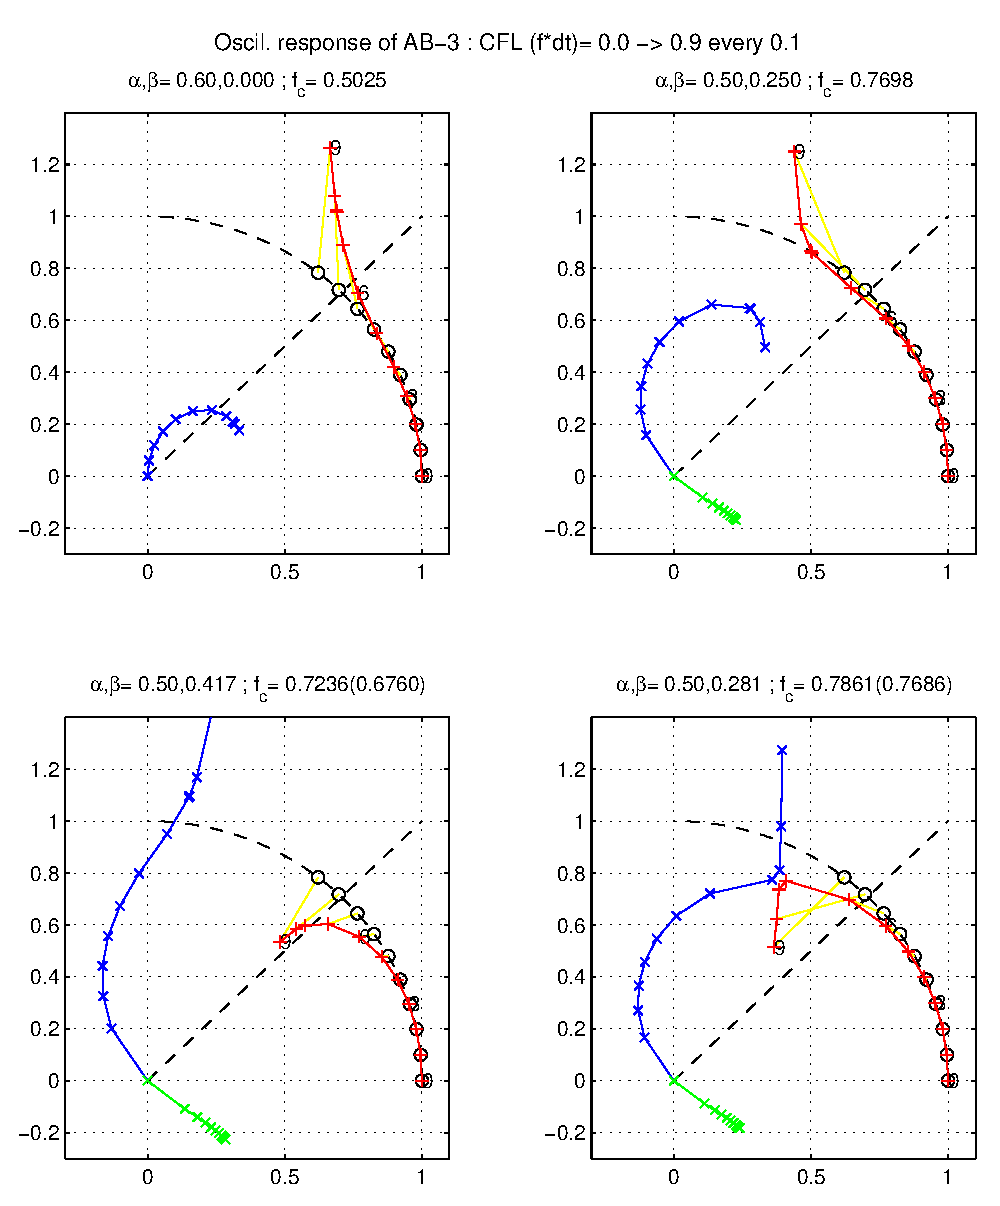
\includegraphics{under_dvlp/stab_AB3_oscil.eps}}
\end{center}
\caption{
Comparison of the oscillatory response of Adams-Bashforth scheme.
}
\label{fig:ab_oscill_response}
\end{figure}

The third-order Adams-Bashforth time stepping (AB-3) provides
several advantages (see, e.g., \cite{durr:91}) compared to
the default quasi-second order Adams-Bashforth (AB-2):
\begin{itemize}
\item higher accuracy;
\item stable with a longer time-step;
\item no additional computation (just requires the storage of one additional 
 time level).
\end{itemize}

The $3^{rd}$ order Adams-Bashforth can be used to 
extrapolate forward in time the tendency
(replacing equation \ref{eq:adams-bashforth2}) 
which writes:
\begin{equation}
G_\tau^{(n+1/2)} = ( 1 + \alpha_{AB} + \beta_{AB}) G_\tau^n
- ( \alpha_{AB} + 2 \beta_{AB}) G_\tau^{n-1}
+ \beta_{AB} G_\tau^{n-2}
\label{eq:adams-bashforth3}
\end{equation}
The 3rd order AB is obtained 
with $(\alpha_{AB},\,\beta_{AB}) = (1/2,\,5/12)$.
Note that selecting 
$(\alpha_{AB},\,\beta_{AB}) = (1/2+\epsilon_{AB},\,0)$
one recovers the quasi-2nd order AB.
%as illustrated on fig.\ref{fig:adams-bashforth-respons}.

The AB-3 time stepping improves the stability limit
for an oscillatory problem like advection or Coriolis. 
As seen from Fig.\ref{fig:ab_oscill_response},
it remains stable up to a CFL of 0.72, 
compared to only 0.50 with AB-2 and $\epsilon_{AB} = 0.1$.
%
It is interesting to note that the stability limit can be further
extended up to a CFL of 0.786 for an oscillatory problem 
(see fig.\ref{fig:ab_oscill_response})
using $(\alpha_{AB},\,\beta_{AB}) = (0.5,\,0.2811)$
but then the scheme is only 2nd order accurate.

\begin{figure}[ht]
\begin{center}
\resizebox{10cm}{!}{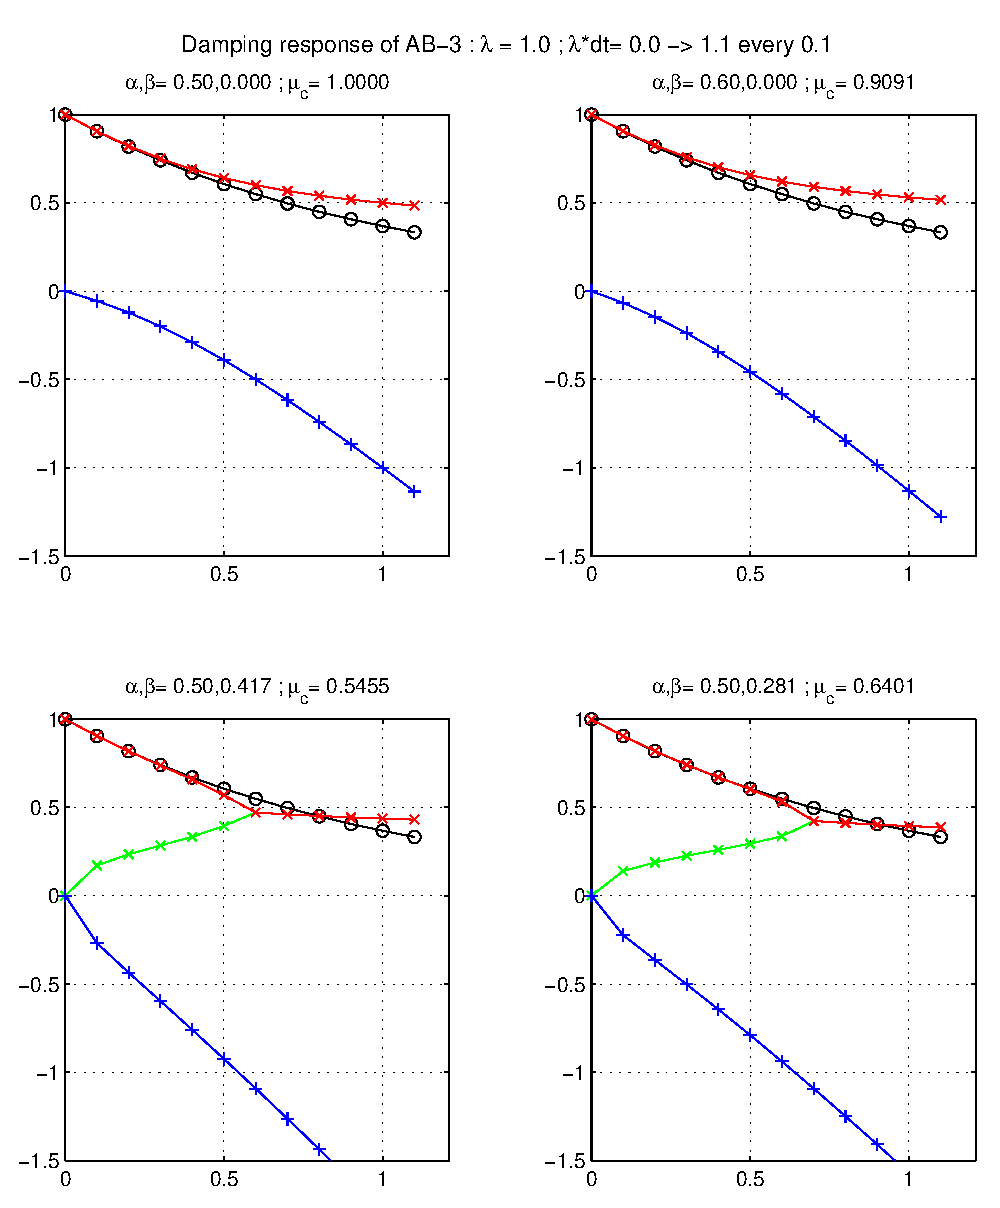
\includegraphics{under_dvlp/stab_AB3_dampR.eps}}
\end{center}
\caption{
Comparison of the damping (diffusion like) response of Adams-Bashforth schemes.
}
\label{fig:ab_damp_response}
\end{figure}

However, the behavior of the AB-3 for a damping problem (like diffusion)
is less favorable, since the stability limit is reduced to 
0.54 only (and 0.64 with $\beta_{AB} = 0.2811$) compared to 1. (and 0.9 
with $\epsilon_{AB} = 0.1$) with the AB-2 (see fig.\ref{fig:ab_damp_response}).

A way to enable the use of a longer time step is
to keep the dissipation terms outside the AB extrapolation
(setting {\em momDissip\_In\_AB=.FALSE.} in main parameter file 
"\texttt{data}", namelist {\em PARM03}),
thus returning to a simple forward time-stepping for dissipation,
and to use AB-3 only for advection and Coriolis terms.

The AB-3 time stepping is activated by defining the option
{\em \#define ALLOW\_ADAMSBASHFORTH\_3}
in "\texttt{CPP\_OPTIONS.h}".
The parameters $\alpha_{AB},\beta_{AB}$ can be set from the
main parameter file "\texttt{data}" (namelist {\em PARM03}) and their 
default value corresponds to the 3rd order Adams-Bashforth.
A simple example is provided in "\texttt{verification/advect\_xy/input.ab3\_c4}".

The AB-3 is not yet available for 
the vertical momentum equation (Non-Hydrostatic) 
neither for passive tracers.

\subsection{Time-extrapolation of tracer (rather than tendency)}
 (to be continued ...)


%\newpage

%\input{s_under_dvlp/text/tracer_dvlp}



% Section: Model Uses
% $Header: /u/gcmpack/manual/model_uses.tex,v 1.5 2006/04/07 02:35:23 edhill Exp $
% $Name:  $

\chapter{Previous Applications of MITgcm}
\label{chap:previous_applications}
\begin{rawhtml}
<!-- CMIREDIR:model_uses_list: -->
\end{rawhtml}



To date, MITgcm has been used for number of purposes.  The following
papers are an incomplete yet fairly broad sample of MITgcm
applications:

\begin{itemize}

\item R.S. Gross and I. Fukumori and D. Menemenlis (2003).
Atmospheric and oceanic excitation of the Earth's wobbles during 1980-2000.
{\it Journal of Geophysical Research-Solid Earth}, vol.108.

\item M.A. Spall and R.S. Pickart (2003).
Wind-driven recirculations and exchange in the Labrador and Irminger Seas. 
{\it Journal of Physical Oceanography}, vol.33, pp.1829--1845. 

\item B. Ferron and J. Marotzke (2003).
Impact of 4D-variational assimilation of WOCE hydrography on the
meridional circulation of the Indian Ocean. {\it Deep-Sea Research Part
II-Topical Studies in Oceanography}, vol.50, pp.2005--2021.

\item G.A. McKinley and M.J. Follows and J. Marshall and S.M. Fan (2003).
Interannual variability of air-sea O-2 fluxes and the determination of
CO2 sinks using atmospheric O-2/N-2. {\it Geophysical Research Letters},
vol.30. 

\item B.Y. Huang and P.H. Stone and A.P. Sokolov and I.V. Kamenkovich
(2003). The deep-ocean heat uptake in transient climate change. {\it Journal
of Climate}, vol.16, pp.1352--1363. 

\item G. de Coetlogon and C. Frankignoul (2003). The persistence of winter
sea surface temperature in the North Atlantic. {\it Journal of Climate},
vol.16, pp.1364--1377. 

\item K.H. Nisancioglu and M.E. Raymo and P.H. Stone (2003).
Reorganization of Miocene deep water circulation in response to the
shoaling of the Central American Seaway. {\it Paleoceanography}, vol.18. 

\item T. Radko and J. Marshall (2003). Equilibration of a Warm Pumped Lens
on a beta plane. {\it Journal of Physical Oceanography}, vol.33, pp.885--899. 

\item T. Stipa (2002). The dynamics of the N/P ratio and stratification in
a large nitrogen-limited estuary as a result of upwelling: a tendency
for offshore Nodularia blooms. {\it Hydrobiologia}, vol.487, pp.219--227. 

\item D. Stammer and C. Wunsch and R. Giering and C. Eckert and P.
Heimbach and J. Marotzke and A. Adcroft and C.N. Hill and J. Marshall
(2003). Volume, heat, and freshwater transports of the global ocean
circulation 1993-2000, estimated from a general circulation model
constrained by World Ocean Circulation Experiment (WOCE) data. {\it Journal
of Geophysical Research-Oceans}, vol.108. 

\item P. Heimbach and C. Hill and R. Giering (2002). Automatic generation
of efficient adjoint code for a parallel Navier-Stokes solver.
{\it Computational Science-ICCS 2002, PT II, Proceedings}, vol.2330,
pp.1019--1028. 

\item D. Stammer and C. Wunsch and R. Giering and C. Eckert and P.
Heimbach and J. Marotzke and A. Adcroft and C.N. Hill and J. Marshall
(2002). Global ocean circulation during 1992-1997, estimated from ocean
observations and a general circulation model. {\it Journal of Geophysical
Research-Oceans}, vol.107. 

\item M. Solovev and P.H. Stone and P. Malanotte-Rizzoli (2002).
Assessment of mesoscale eddy parameterizations for a single-basin
coarse-resolution ocean model. {\it Journal of Geophysical Research-Oceans},
vol.107. 

\item C. Herbaut and J. Sirven and S. Fevrier (2002). Response of a
simplified oceanic general circulation model to idealized NAO-like
stochastic forcing. {\it Journal of Physical Oceanography}, vol.32,
pp.3182--3192. 

\item C. Wunsch (2002). Oceanic age and transient tracers: Analytical and
numerical solutions. {\it Journal of Geophysical Research-Oceans}, vol.107. 

\item J. Sirven and C. Frankignoul and D. de Coetlogon and V. Taillandier
(2002). Spectrum of wind-driven baroclinic fluctuations of the ocean in
the midlatitudes. {\it Journal of Physical Oceanography}, vol.32,
pp.2405--2417. 

\item R. Zhang and M. Follows and J. Marshall (2002). Mechanisms of
thermohaline mode switching with application to warm equable climates.
{\it Journal of Climate}, vol.15, pp.2056--2072. 

\item G. Brostrom (2002). On advection and diffusion of plankton in coarse
resolution ocean models. {\it Journal of Marine Systems}, vol.35, pp.99--110. 

\item T. Lee and I. Fukumori and D. Menemenlis and Z.F. Xing and L.L. Fu
(2002). Effects of the Indonesian Throughflow on the Pacific and Indian
oceans. {\it Journal of Physical Oceanography}, vol.32, pp.1404--1429. 


\item C. Herbaut and J. Marshall (2002). Mechanisms of buoyancy transport
through mixed layers and statistical signatures from isobaric floats.
{\it Journal of Physical Oceanography}, vol.32, pp.545--557. 

\item J. Marshall and H. Jones and R. Karsten and R. Wardle (2002). Can
eddies set ocean stratification?, {\it Journal of Physical Oceanography},
vol.32, pp.26--38. 

\item C. Herbaut and J. Sirven and A. Czaja (2001). An idealized model
study of the mass and heat transports between the subpolar and
subtropical gyres. {\it Journal of Physical Oceanography}, vol.31,
pp.2903--2916. 

\item R.H. Kase and A. Biastoch and D.B. Stammer (2001). On the Mid-Depth
Circulation in the Labrador and Irminger Seas. {\it Geophysical Research
Letters}, vol.28, pp.3433--3436. 

\item R. Zhang and M.J. Follows and J.P. Grotzinger and J. Marshall
(2001). Could the Late Permian deep ocean have been anoxic?.
{\it Paleoceanography}, vol.16, pp.317--329. 

\item A. Adcroft and J.R. Scott and J. Marotzke (2001). Impact of
geothermal heating on the global ocean circulation. {\it Geophysical Research
Letters}, vol.28, pp.1735--1738. 

\item J. Marshall and D. Jamous and J. Nilsson (2001). Entry, flux, and
exit of potential vorticity in ocean circulation. {\it Journal of Physical
Oceanography}, vol.31, pp.777--789. 

\item A. Mahadevan (2001). An analysis of bomb radiocarbon trends in the
Pacific. {\it Marine Chemistry}, vol.73, pp.273--290. 


\item G. Brostrom (2000). The role of the annual cycles for the air-sea
exchange of CO2. {\it Marine Chemistry}, vol.72, pp.151--169. 

\item Y.H. Zhou and H.Q. Wu and N.H. Yu and D.W. Zheng (2000). Excitation
of seasonal polar motion by atmospheric and oceanic angular momentums.
{\it Progress in Natural Science}, vol.10, pp.931--936. 

\item R. Wardle and J. Marshall (2000). Representation of eddies in
primitive equation models by a PV flux. {\it Journal of Physical
Oceanography}, vol.30, pp.2481--2503. 

\item P.S. Polito and O.T. Sato and W.T. Liu (2000). Characterization and
validation of the heat storage variability from TOPEX/Poseidon at four
oceanographic sites. {\it Journal of Geophysical Research-Oceans}, vol.105,
pp.16911--16921. 

\item R.M. Ponte and D. Stammer (2000). Global and regional axial ocean
angular momentum signals and length-of-day variations (1985-1996).
{\it Journal of Geophysical Research-Oceans}, vol.105, pp.17161--17171. 

\item J. Wunsch (2000). Oceanic influence on the annual polar motion.
{\it Journal of GEODYNAMICS}, vol.30, pp.389--399. 

\item D. Menemenlis and M. Chechelnitsky (2000). Error estimates for an
ocean general circulation model from altimeter and acoustic tomography
data. {\it Monthly Weather Review}, vol.128, pp.763--778. 

\item Y.H. Zhou and D.W. Zheng and N.H. Yu and H.Q. Wu (2000). Excitation
of annual polar motion by atmosphere and ocean. {\it Chinese Science
Bulletin}, vol.45, pp.139--142. 

\item J. Marotzke and R. Giering and K.Q. Zhang and D. Stammer and C. Hill
and T. Lee (1999). Construction of the adjoint MIT ocean general
circulation model and application to Atlantic heat transport
sensitivity. {\it Journal of Geophysical Research-Oceans}, vol.104,
pp.29529--29547. 

\item R.M. Ponte and D. Stammer (1999). Role of ocean currents and bottom
pressure variability on seasonal polar motion. {\it Journal of Geophysical
Research-Oceans}, vol.104, pp.23393--23409. 

\item J. Nastula and R.M. Ponte (1999). Further evidence for oceanic
excitation of polar motion. {\it Geophysical Journal International}, vol.139,
pp.123--130. 

\item K.Q. Zhang and J. Marotzke (1999). The importance of open-boundary
estimation for an Indian Ocean GCM-data synthesis. {\it Journal of Marine
Research}, vol.57, pp.305--334. 

\item J. Marshall and D. Jamous and J. Nilsson (1999). Reconciling
thermodynamic and dynamic methods of computation of water-mass
transformation rates. {\it Deep-Sea Research PART I-Oceanographic Research
Papers}, vol.46, pp.545--572. 

\item J. Marshall and F. Schott (1999). Open-ocean convection:
Observations, theory, and models. {\it Reviews of Geophysics}, vol.37,
pp.1--64. 

\item J. Marshall and H. Jones and C. Hill (1998). Efficient ocean
modeling using non-hydrostatic algorithms. {\it Journal of Marine Systems},
vol.18, pp.115--134. 

\item A.B. Baggeroer and T.G. Birdsall and C. Clark and J.A. Colosi and
B.D. Cornuelle and D. Costa and B.D. Dushaw and M. Dzieciuch and A.M.G.
Forbes and C. Hill and B.M. Howe and J. Marshall and D. Menemenlis and
J.A. Mercer and K. Metzger and W. Munk and R.C. Spindel and D. Stammer
and P.F. Worcester and C. Wunsch (1998). Ocean climate change:
Comparison of acoustic tomography, satellite altimetry, and modeling.
{\it Science}, vol.281, pp.1327--1332. 

\item C. Wunsch and D. Stammer (1998). Satellite altimetry, the marine
geoid, and the oceanic general circulation. {\it Annual Review of Earth and
Planetary Sciences}, vol.26, pp.219--253. 

\item A. Shaw and Arvind and K.C. Cho and C. Hill and R.P. Johnson and J.
Marshall (1998). A comparison of implicitly parallel multithreaded and
data-parallel implementations of an ocean model. {\it Journal of Parallel and
Distributed Computing}, vol.48, pp.1--51. 

\item T.W.N. Haine and J. Marshall (1998). Gravitational, symmetric, and
baroclinic instability of the ocean mixed layer. {\it Journal of Physical
Oceanography}, vol.28, pp.634--658. 

\item R.M. Ponte and D. Stammer and J. Marshall (1998). Oceanic signals in
observed motions of the Earth's pole of rotation. {\it Nature}, vol.391,
pp.476--479. 

\item D. Menemenlis and C. Wunsch (1997). Linearization of an oceanic
general circulation model for data assimilation and climate studies.
{\it Journal of Atmospheric and Oceanic Technology}, vol.14, pp.1420--1443. 

\item H. Jones and J. Marshall (1997). Restratification after deep
convection. {\it Journal of Physical Oceanography}, vol.27, pp.2276--2287. 

\item S.R. Jayne and R. Tokmakian (1997). Forcing and sampling of ocean
general circulation models: Impact of high-frequency motions. {\it Journal of
Physical Oceanography}, vol.27, pp.1173--1179. 

\end{itemize}

%\pagebreak

% Section: References:
%\markboth{BIBLIOGRAPHY}{BIBLIOGRAPHY}
\addcontentsline{toc}{chapter}{BIBLIOGRAPHY}
%aja%\bibliography{\BIBPATH/manual_references}
\bibliography{manual_references,baylor_biblio}

\end{document}
